
\chapter{La détection des anomalies dans les délais d'un lien}

\section{Introduction}

Dans le présent chapitre, nous allons présenter l'outil de détection des anomalies dans les délais d'un lien  conçu dans le cadre du travail de R. Fontugne et al \cite{DBLP:journals/corr/FontugneAPB16}. Nous avons choisi ce travail qui exploite des données massives en vue d'évaluer quelques technologies du Big Data.

\section{Présentation du travail de référence}

\paragraph{Une vue globale du travail de référence}~ 

Le travail de R. Fontugne \cite{DBLP:journals/corr/FontugneAPB16} et al exploite une des mesures effectuées par les sondes Atlas, c'est la requête traceroute. L'idée de ce travail est de collecter les résultats des requêtes traceroutes effectuées par les sondes Atlas, ensuite comparer la référence avec la valeur courante. Cette  référence pour le délai  d'un lien donné   sera mise à jour au fur et à mesure de l'analyse.

\section{Présentation de l'outil de la détection des anomalies }

Les entrées de l'algorithme de la détection est un ensemble de traceroutes. Un traceroute (Traceroute) est un ensemble de sauts (Hop) en plus les informations générales concernant la sonde ayant effectué la requête traceroute et la destination de la requête. Chaque saut est décrit par un ensemble de signaux (Signal), où un signal, dans le présent contexte, décrit le routeur ayant émet une réponse à la sonde Atlas parmi les routeurs traversés avant d'atteindre la destination finale.  Pour le saut $i$, on note trois signaux dont le routeur émettant le signal est $fromij$ avec un RTT égal à $rttij$, avec $j \in [1,3]$ comme illustré dans la figure \ref{fig:traceroute}.

\begin{figure}[H]
	\centering
	\resizebox{\textwidth}{!}{
	% Graphic for TeX using PGF
% Title: /home/bellafkih/Documents/2018-2019/memoire/rapport_memoire/dia/traceroute.dia
% Creator: Dia v0.97.3
% CreationDate: Sun Sep 23 22:12:05 2018
% For: bellafkih
% \usepackage{tikz}
% The following commands are not supported in PSTricks at present
% We define them conditionally, so when they are implemented,
% this pgf file will use them.
\ifx\du\undefined
  \newlength{\du}
\fi
\setlength{\du}{15\unitlength}
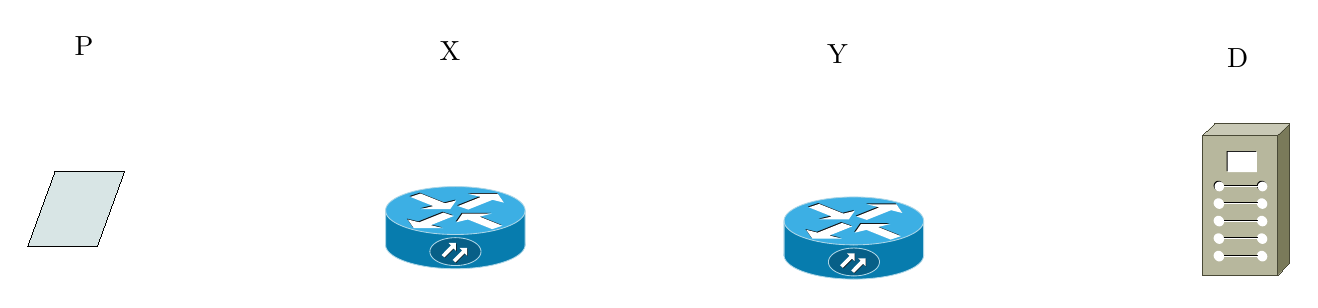
\begin{tikzpicture}
\pgftransformxscale{1.000000}
\pgftransformyscale{-1.000000}
\definecolor{dialinecolor}{rgb}{0.000000, 0.000000, 0.000000}
\pgfsetstrokecolor{dialinecolor}
\definecolor{dialinecolor}{rgb}{1.000000, 1.000000, 1.000000}
\pgfsetfillcolor{dialinecolor}
\definecolor{dialinecolor}{rgb}{0.847059, 0.898039, 0.898039}
\pgfsetfillcolor{dialinecolor}
\fill (6.953088\du,8.550000\du)--(8.629264\du,8.550000\du)--(7.974118\du,10.350000\du)--(6.297942\du,10.350000\du)--cycle;
\pgfsetlinewidth{0.000000\du}
\pgfsetdash{}{0pt}
\pgfsetdash{}{0pt}
\pgfsetmiterjoin
\definecolor{dialinecolor}{rgb}{0.000000, 0.000000, 0.000000}
\pgfsetstrokecolor{dialinecolor}
\draw (6.953088\du,8.550000\du)--(8.629264\du,8.550000\du)--(7.974118\du,10.350000\du)--(6.297942\du,10.350000\du)--cycle;
% setfont left to latex
\definecolor{dialinecolor}{rgb}{0.000000, 0.000000, 0.000000}
\pgfsetstrokecolor{dialinecolor}
\node at (7.463603\du,9.645000\du){};
\pgfsetlinewidth{0.000000\du}
\pgfsetdash{}{0pt}
\pgfsetdash{}{0pt}
\pgfsetbuttcap
\pgfsetmiterjoin
\pgfsetlinewidth{0.000000\du}
\pgfsetbuttcap
\pgfsetmiterjoin
\pgfsetdash{}{0pt}
\definecolor{dialinecolor}{rgb}{0.027451, 0.486275, 0.682353}
\pgfsetfillcolor{dialinecolor}
\pgfpathmoveto{\pgfpoint{18.279993\du}{10.312559\du}}
\pgfpathlineto{\pgfpoint{18.278532\du}{10.341767\du}}
\pgfpathlineto{\pgfpoint{18.271230\du}{10.371705\du}}
\pgfpathlineto{\pgfpoint{18.261008\du}{10.400183\du}}
\pgfpathlineto{\pgfpoint{18.246404\du}{10.428295\du}}
\pgfpathlineto{\pgfpoint{18.227054\du}{10.456407\du}}
\pgfpathlineto{\pgfpoint{18.205148\du}{10.483790\du}}
\pgfpathlineto{\pgfpoint{18.178496\du}{10.510807\du}}
\pgfpathlineto{\pgfpoint{18.147828\du}{10.537094\du}}
\pgfpathlineto{\pgfpoint{18.114969\du}{10.562286\du}}
\pgfpathlineto{\pgfpoint{18.077729\du}{10.587477\du}}
\pgfpathlineto{\pgfpoint{18.036838\du}{10.611574\du}}
\pgfpathlineto{\pgfpoint{17.993027\du}{10.634940\du}}
\pgfpathlineto{\pgfpoint{17.946659\du}{10.657576\du}}
\pgfpathlineto{\pgfpoint{17.896276\du}{10.679482\du}}
\pgfpathlineto{\pgfpoint{17.843337\du}{10.700292\du}}
\pgfpathlineto{\pgfpoint{17.787842\du}{10.720372\du}}
\pgfpathlineto{\pgfpoint{17.729792\du}{10.739723\du}}
\pgfpathlineto{\pgfpoint{17.669186\du}{10.757612\du}}
\pgfpathlineto{\pgfpoint{17.605294\du}{10.774772\du}}
\pgfpathlineto{\pgfpoint{17.540307\du}{10.791201\du}}
\pgfpathlineto{\pgfpoint{17.471668\du}{10.806170\du}}
\pgfpathlineto{\pgfpoint{17.400840\du}{10.819679\du}}
\pgfpathlineto{\pgfpoint{17.328916\du}{10.832457\du}}
\pgfpathlineto{\pgfpoint{17.254071\du}{10.844505\du}}
\pgfpathlineto{\pgfpoint{17.178131\du}{10.854363\du}}
\pgfpathlineto{\pgfpoint{17.099635\du}{10.863490\du}}
\pgfpathlineto{\pgfpoint{17.020044\du}{10.871157\du}}
\pgfpathlineto{\pgfpoint{16.938992\du}{10.877729\du}}
\pgfpathlineto{\pgfpoint{16.855750\du}{10.882840\du}}
\pgfpathlineto{\pgfpoint{16.772143\du}{10.886491\du}}
\pgfpathlineto{\pgfpoint{16.686710\du}{10.888682\du}}
\pgfpathlineto{\pgfpoint{16.600183\du}{10.889412\du}}
\pgfpathlineto{\pgfpoint{16.514020\du}{10.888682\du}}
\pgfpathlineto{\pgfpoint{16.428222\du}{10.886491\du}}
\pgfpathlineto{\pgfpoint{16.344615\du}{10.882840\du}}
\pgfpathlineto{\pgfpoint{16.261738\du}{10.877729\du}}
\pgfpathlineto{\pgfpoint{16.180321\du}{10.871157\du}}
\pgfpathlineto{\pgfpoint{16.100730\du}{10.863490\du}}
\pgfpathlineto{\pgfpoint{16.022965\du}{10.854363\du}}
\pgfpathlineto{\pgfpoint{15.946294\du}{10.844505\du}}
\pgfpathlineto{\pgfpoint{15.872180\du}{10.832457\du}}
\pgfpathlineto{\pgfpoint{15.799525\du}{10.819679\du}}
\pgfpathlineto{\pgfpoint{15.729062\du}{10.806170\du}}
\pgfpathlineto{\pgfpoint{15.660424\du}{10.791201\du}}
\pgfpathlineto{\pgfpoint{15.594706\du}{10.774772\du}}
\pgfpathlineto{\pgfpoint{15.531179\du}{10.757612\du}}
\pgfpathlineto{\pgfpoint{15.470208\du}{10.739723\du}}
\pgfpathlineto{\pgfpoint{15.411793\du}{10.720372\du}}
\pgfpathlineto{\pgfpoint{15.356663\du}{10.700292\du}}
\pgfpathlineto{\pgfpoint{15.303724\du}{10.679482\du}}
\pgfpathlineto{\pgfpoint{15.253706\du}{10.657576\du}}
\pgfpathlineto{\pgfpoint{15.206608\du}{10.634940\du}}
\pgfpathlineto{\pgfpoint{15.163162\du}{10.611574\du}}
\pgfpathlineto{\pgfpoint{15.122271\du}{10.587477\du}}
\pgfpathlineto{\pgfpoint{15.085031\du}{10.562286\du}}
\pgfpathlineto{\pgfpoint{15.051807\du}{10.537094\du}}
\pgfpathlineto{\pgfpoint{15.021504\du}{10.510807\du}}
\pgfpathlineto{\pgfpoint{14.994852\du}{10.483790\du}}
\pgfpathlineto{\pgfpoint{14.972946\du}{10.456407\du}}
\pgfpathlineto{\pgfpoint{14.953596\du}{10.428295\du}}
\pgfpathlineto{\pgfpoint{14.938992\du}{10.400183\du}}
\pgfpathlineto{\pgfpoint{14.928405\du}{10.371705\du}}
\pgfpathlineto{\pgfpoint{14.921468\du}{10.341767\du}}
\pgfpathlineto{\pgfpoint{14.919642\du}{10.312559\du}}
\pgfpathlineto{\pgfpoint{14.921468\du}{10.282621\du}}
\pgfpathlineto{\pgfpoint{14.928405\du}{10.253414\du}}
\pgfpathlineto{\pgfpoint{14.938992\du}{10.224206\du}}
\pgfpathlineto{\pgfpoint{14.953596\du}{10.196093\du}}
\pgfpathlineto{\pgfpoint{14.972946\du}{10.167981\du}}
\pgfpathlineto{\pgfpoint{14.994852\du}{10.140599\du}}
\pgfpathlineto{\pgfpoint{15.021504\du}{10.113947\du}}
\pgfpathlineto{\pgfpoint{15.051807\du}{10.087660\du}}
\pgfpathlineto{\pgfpoint{15.085031\du}{10.062103\du}}
\pgfpathlineto{\pgfpoint{15.122271\du}{10.037276\du}}
\pgfpathlineto{\pgfpoint{15.163162\du}{10.012815\du}}
\pgfpathlineto{\pgfpoint{15.206608\du}{9.989449\du}}
\pgfpathlineto{\pgfpoint{15.253706\du}{9.967178\du}}
\pgfpathlineto{\pgfpoint{15.303724\du}{9.944907\du}}
\pgfpathlineto{\pgfpoint{15.356663\du}{9.924096\du}}
\pgfpathlineto{\pgfpoint{15.411793\du}{9.904016\du}}
\pgfpathlineto{\pgfpoint{15.470208\du}{9.885396\du}}
\pgfpathlineto{\pgfpoint{15.531179\du}{9.866411\du}}
\pgfpathlineto{\pgfpoint{15.594706\du}{9.849617\du}}
\pgfpathlineto{\pgfpoint{15.660424\du}{9.833917\du}}
\pgfpathlineto{\pgfpoint{15.729062\du}{9.818583\du}}
\pgfpathlineto{\pgfpoint{15.799525\du}{9.804710\du}}
\pgfpathlineto{\pgfpoint{15.872180\du}{9.791566\du}}
\pgfpathlineto{\pgfpoint{15.946294\du}{9.780613\du}}
\pgfpathlineto{\pgfpoint{16.022965\du}{9.770026\du}}
\pgfpathlineto{\pgfpoint{16.100730\du}{9.760533\du}}
\pgfpathlineto{\pgfpoint{16.180321\du}{9.753231\du}}
\pgfpathlineto{\pgfpoint{16.261738\du}{9.746659\du}}
\pgfpathlineto{\pgfpoint{16.344615\du}{9.741548\du}}
\pgfpathlineto{\pgfpoint{16.428222\du}{9.737897\du}}
\pgfpathlineto{\pgfpoint{16.514020\du}{9.736072\du}}
\pgfpathlineto{\pgfpoint{16.600183\du}{9.734976\du}}
\pgfpathlineto{\pgfpoint{16.686710\du}{9.736072\du}}
\pgfpathlineto{\pgfpoint{16.772143\du}{9.737897\du}}
\pgfpathlineto{\pgfpoint{16.855750\du}{9.741548\du}}
\pgfpathlineto{\pgfpoint{16.938992\du}{9.746659\du}}
\pgfpathlineto{\pgfpoint{17.020044\du}{9.753231\du}}
\pgfpathlineto{\pgfpoint{17.099635\du}{9.760533\du}}
\pgfpathlineto{\pgfpoint{17.178131\du}{9.770026\du}}
\pgfpathlineto{\pgfpoint{17.254071\du}{9.780613\du}}
\pgfpathlineto{\pgfpoint{17.328916\du}{9.791566\du}}
\pgfpathlineto{\pgfpoint{17.400840\du}{9.804710\du}}
\pgfpathlineto{\pgfpoint{17.471668\du}{9.818583\du}}
\pgfpathlineto{\pgfpoint{17.540307\du}{9.833917\du}}
\pgfpathlineto{\pgfpoint{17.605294\du}{9.849617\du}}
\pgfpathlineto{\pgfpoint{17.669186\du}{9.866411\du}}
\pgfpathlineto{\pgfpoint{17.729792\du}{9.885396\du}}
\pgfpathlineto{\pgfpoint{17.787842\du}{9.904016\du}}
\pgfpathlineto{\pgfpoint{17.843337\du}{9.924096\du}}
\pgfpathlineto{\pgfpoint{17.896276\du}{9.944907\du}}
\pgfpathlineto{\pgfpoint{17.946659\du}{9.967178\du}}
\pgfpathlineto{\pgfpoint{17.993027\du}{9.989449\du}}
\pgfpathlineto{\pgfpoint{18.036838\du}{10.012815\du}}
\pgfpathlineto{\pgfpoint{18.077729\du}{10.037276\du}}
\pgfpathlineto{\pgfpoint{18.114969\du}{10.062103\du}}
\pgfpathlineto{\pgfpoint{18.147828\du}{10.087660\du}}
\pgfpathlineto{\pgfpoint{18.178496\du}{10.113947\du}}
\pgfpathlineto{\pgfpoint{18.205148\du}{10.140599\du}}
\pgfpathlineto{\pgfpoint{18.227054\du}{10.167981\du}}
\pgfpathlineto{\pgfpoint{18.246404\du}{10.196093\du}}
\pgfpathlineto{\pgfpoint{18.261008\du}{10.224206\du}}
\pgfpathlineto{\pgfpoint{18.271230\du}{10.253414\du}}
\pgfpathlineto{\pgfpoint{18.278532\du}{10.282621\du}}
\pgfpathlineto{\pgfpoint{18.279993\du}{10.312559\du}}
\pgfusepath{fill}
\pgfsetlinewidth{0.000000\du}
\pgfsetbuttcap
\pgfsetmiterjoin
\pgfsetdash{}{0pt}
\definecolor{dialinecolor}{rgb}{0.678431, 0.839216, 0.905882}
\pgfsetfillcolor{dialinecolor}
\pgfpathmoveto{\pgfpoint{16.600183\du}{10.900000\du}}
\pgfpathlineto{\pgfpoint{16.600183\du}{10.900000\du}}
\pgfpathlineto{\pgfpoint{16.643629\du}{10.900000\du}}
\pgfpathlineto{\pgfpoint{16.687076\du}{10.899270\du}}
\pgfpathlineto{\pgfpoint{16.730157\du}{10.898175\du}}
\pgfpathlineto{\pgfpoint{16.772143\du}{10.897079\du}}
\pgfpathlineto{\pgfpoint{16.814859\du}{10.895254\du}}
\pgfpathlineto{\pgfpoint{16.856480\du}{10.893063\du}}
\pgfpathlineto{\pgfpoint{16.898101\du}{10.890507\du}}
\pgfpathlineto{\pgfpoint{16.939723\du}{10.888317\du}}
\pgfpathlineto{\pgfpoint{16.980248\du}{10.885396\du}}
\pgfpathlineto{\pgfpoint{17.021139\du}{10.881745\du}}
\pgfpathlineto{\pgfpoint{17.060935\du}{10.877729\du}}
\pgfpathlineto{\pgfpoint{17.101095\du}{10.873713\du}}
\pgfpathlineto{\pgfpoint{17.139796\du}{10.869332\du}}
\pgfpathlineto{\pgfpoint{17.179226\du}{10.864951\du}}
\pgfpathlineto{\pgfpoint{17.217196\du}{10.859474\du}}
\pgfpathlineto{\pgfpoint{17.256261\du}{10.854363\du}}
\pgfpathlineto{\pgfpoint{17.293501\du}{10.848886\du}}
\pgfpathlineto{\pgfpoint{17.330376\du}{10.842680\du}}
\pgfpathlineto{\pgfpoint{17.366886\du}{10.836838\du}}
\pgfpathlineto{\pgfpoint{17.403395\du}{10.830267\du}}
\pgfpathlineto{\pgfpoint{17.438810\du}{10.823330\du}}
\pgfpathlineto{\pgfpoint{17.473494\du}{10.816393\du}}
\pgfpathlineto{\pgfpoint{17.508178\du}{10.808726\du}}
\pgfpathlineto{\pgfpoint{17.542132\du}{10.801059\du}}
\pgfpathlineto{\pgfpoint{17.575721\du}{10.792662\du}}
\pgfpathlineto{\pgfpoint{17.608580\du}{10.784629\du}}
\pgfpathlineto{\pgfpoint{17.640343\du}{10.776597\du}}
\pgfpathlineto{\pgfpoint{17.671742\du}{10.767835\du}}
\pgfpathlineto{\pgfpoint{17.687076\du}{10.763089\du}}
\pgfpathlineto{\pgfpoint{17.702410\du}{10.759073\du}}
\pgfpathlineto{\pgfpoint{17.718474\du}{10.754326\du}}
\pgfpathlineto{\pgfpoint{17.733078\du}{10.749580\du}}
\pgfpathlineto{\pgfpoint{17.747317\du}{10.744834\du}}
\pgfpathlineto{\pgfpoint{17.762286\du}{10.739723\du}}
\pgfpathlineto{\pgfpoint{17.777254\du}{10.734976\du}}
\pgfpathlineto{\pgfpoint{17.791128\du}{10.730230\du}}
\pgfpathlineto{\pgfpoint{17.805367\du}{10.725119\du}}
\pgfpathlineto{\pgfpoint{17.819241\du}{10.720372\du}}
\pgfpathlineto{\pgfpoint{17.833479\du}{10.714896\du}}
\pgfpathlineto{\pgfpoint{17.846623\du}{10.710515\du}}
\pgfpathlineto{\pgfpoint{17.860862\du}{10.705038\du}}
\pgfpathlineto{\pgfpoint{17.874005\du}{10.699927\du}}
\pgfpathlineto{\pgfpoint{17.887149\du}{10.694451\du}}
\pgfpathlineto{\pgfpoint{17.900657\du}{10.688609\du}}
\pgfpathlineto{\pgfpoint{17.913436\du}{10.683498\du}}
\pgfpathlineto{\pgfpoint{17.925484\du}{10.678021\du}}
\pgfpathlineto{\pgfpoint{17.938262\du}{10.672180\du}}
\pgfpathlineto{\pgfpoint{17.950675\du}{10.667068\du}}
\pgfpathlineto{\pgfpoint{17.963089\du}{10.661227\du}}
\pgfpathlineto{\pgfpoint{17.974407\du}{10.655750\du}}
\pgfpathlineto{\pgfpoint{17.986455\du}{10.649909\du}}
\pgfpathlineto{\pgfpoint{17.997408\du}{10.644067\du}}
\pgfpathlineto{\pgfpoint{18.009091\du}{10.638226\du}}
\pgfpathlineto{\pgfpoint{18.020409\du}{10.632384\du}}
\pgfpathlineto{\pgfpoint{18.031727\du}{10.626543\du}}
\pgfpathlineto{\pgfpoint{18.042315\du}{10.620336\du}}
\pgfpathlineto{\pgfpoint{18.052172\du}{10.614494\du}}
\pgfpathlineto{\pgfpoint{18.062760\du}{10.608653\du}}
\pgfpathlineto{\pgfpoint{18.072983\du}{10.602081\du}}
\pgfpathlineto{\pgfpoint{18.082840\du}{10.596240\du}}
\pgfpathlineto{\pgfpoint{18.092698\du}{10.589668\du}}
\pgfpathlineto{\pgfpoint{18.101825\du}{10.583461\du}}
\pgfpathlineto{\pgfpoint{18.110953\du}{10.576889\du}}
\pgfpathlineto{\pgfpoint{18.120445\du}{10.571048\du}}
\pgfpathlineto{\pgfpoint{18.129208\du}{10.564476\du}}
\pgfpathlineto{\pgfpoint{18.138335\du}{10.558269\du}}
\pgfpathlineto{\pgfpoint{18.146367\du}{10.551698\du}}
\pgfpathlineto{\pgfpoint{18.155130\du}{10.544761\du}}
\pgfpathlineto{\pgfpoint{18.162432\du}{10.538189\du}}
\pgfpathlineto{\pgfpoint{18.170464\du}{10.531982\du}}
\pgfpathlineto{\pgfpoint{18.178496\du}{10.524681\du}}
\pgfpathlineto{\pgfpoint{18.185068\du}{10.518474\du}}
\pgfpathlineto{\pgfpoint{18.192369\du}{10.511537\du}}
\pgfpathlineto{\pgfpoint{18.198941\du}{10.504235\du}}
\pgfpathlineto{\pgfpoint{18.205878\du}{10.498028\du}}
\pgfpathlineto{\pgfpoint{18.212450\du}{10.491092\du}}
\pgfpathlineto{\pgfpoint{18.218656\du}{10.483790\du}}
\pgfpathlineto{\pgfpoint{18.224498\du}{10.476853\du}}
\pgfpathlineto{\pgfpoint{18.229974\du}{10.469916\du}}
\pgfpathlineto{\pgfpoint{18.235816\du}{10.462979\du}}
\pgfpathlineto{\pgfpoint{18.240562\du}{10.455677\du}}
\pgfpathlineto{\pgfpoint{18.246039\du}{10.448375\du}}
\pgfpathlineto{\pgfpoint{18.250785\du}{10.441073\du}}
\pgfpathlineto{\pgfpoint{18.255166\du}{10.434137\du}}
\pgfpathlineto{\pgfpoint{18.259182\du}{10.426470\du}}
\pgfpathlineto{\pgfpoint{18.263198\du}{10.419533\du}}
\pgfpathlineto{\pgfpoint{18.266484\du}{10.411866\du}}
\pgfpathlineto{\pgfpoint{18.270500\du}{10.404199\du}}
\pgfpathlineto{\pgfpoint{18.273786\du}{10.396532\du}}
\pgfpathlineto{\pgfpoint{18.276342\du}{10.389230\du}}
\pgfpathlineto{\pgfpoint{18.279263\du}{10.381928\du}}
\pgfpathlineto{\pgfpoint{18.281088\du}{10.374626\du}}
\pgfpathlineto{\pgfpoint{18.284009\du}{10.366959\du}}
\pgfpathlineto{\pgfpoint{18.285104\du}{10.358562\du}}
\pgfpathlineto{\pgfpoint{18.287295\du}{10.350894\du}}
\pgfpathlineto{\pgfpoint{18.288390\du}{10.343593\du}}
\pgfpathlineto{\pgfpoint{18.289120\du}{10.335926\du}}
\pgfpathlineto{\pgfpoint{18.289850\du}{10.327528\du}}
\pgfpathlineto{\pgfpoint{18.290581\du}{10.320226\du}}
\pgfpathlineto{\pgfpoint{18.290581\du}{10.312559\du}}
\pgfpathlineto{\pgfpoint{18.270500\du}{10.312559\du}}
\pgfpathlineto{\pgfpoint{18.269770\du}{10.319496\du}}
\pgfpathlineto{\pgfpoint{18.269770\du}{10.326433\du}}
\pgfpathlineto{\pgfpoint{18.269405\du}{10.333370\du}}
\pgfpathlineto{\pgfpoint{18.267579\du}{10.340672\du}}
\pgfpathlineto{\pgfpoint{18.266484\du}{10.347609\du}}
\pgfpathlineto{\pgfpoint{18.265754\du}{10.354545\du}}
\pgfpathlineto{\pgfpoint{18.263563\du}{10.361482\du}}
\pgfpathlineto{\pgfpoint{18.262103\du}{10.368784\du}}
\pgfpathlineto{\pgfpoint{18.259912\du}{10.374991\du}}
\pgfpathlineto{\pgfpoint{18.257357\du}{10.381928\du}}
\pgfpathlineto{\pgfpoint{18.254436\du}{10.389230\du}}
\pgfpathlineto{\pgfpoint{18.251880\du}{10.396166\du}}
\pgfpathlineto{\pgfpoint{18.247864\du}{10.403103\du}}
\pgfpathlineto{\pgfpoint{18.244943\du}{10.409675\du}}
\pgfpathlineto{\pgfpoint{18.240927\du}{10.416612\du}}
\pgfpathlineto{\pgfpoint{18.238007\du}{10.423184\du}}
\pgfpathlineto{\pgfpoint{18.233625\du}{10.430120\du}}
\pgfpathlineto{\pgfpoint{18.229244\du}{10.437057\du}}
\pgfpathlineto{\pgfpoint{18.224498\du}{10.443629\du}}
\pgfpathlineto{\pgfpoint{18.219387\du}{10.449836\du}}
\pgfpathlineto{\pgfpoint{18.214640\du}{10.457138\du}}
\pgfpathlineto{\pgfpoint{18.208434\du}{10.464074\du}}
\pgfpathlineto{\pgfpoint{18.202957\du}{10.470281\du}}
\pgfpathlineto{\pgfpoint{18.197846\du}{10.476853\du}}
\pgfpathlineto{\pgfpoint{18.191274\du}{10.483425\du}}
\pgfpathlineto{\pgfpoint{18.184337\du}{10.490361\du}}
\pgfpathlineto{\pgfpoint{18.178496\du}{10.496933\du}}
\pgfpathlineto{\pgfpoint{18.171194\du}{10.503140\du}}
\pgfpathlineto{\pgfpoint{18.164622\du}{10.509712\du}}
\pgfpathlineto{\pgfpoint{18.156955\du}{10.515918\du}}
\pgfpathlineto{\pgfpoint{18.149653\du}{10.522490\du}}
\pgfpathlineto{\pgfpoint{18.141621\du}{10.529062\du}}
\pgfpathlineto{\pgfpoint{18.133954\du}{10.535268\du}}
\pgfpathlineto{\pgfpoint{18.125192\du}{10.541840\du}}
\pgfpathlineto{\pgfpoint{18.116794\du}{10.547682\du}}
\pgfpathlineto{\pgfpoint{18.108032\du}{10.554253\du}}
\pgfpathlineto{\pgfpoint{18.100000\du}{10.560460\du}}
\pgfpathlineto{\pgfpoint{18.091238\du}{10.566302\du}}
\pgfpathlineto{\pgfpoint{18.081745\du}{10.572873\du}}
\pgfpathlineto{\pgfpoint{18.071522\du}{10.578715\du}}
\pgfpathlineto{\pgfpoint{18.062395\du}{10.585287\du}}
\pgfpathlineto{\pgfpoint{18.052172\du}{10.591128\du}}
\pgfpathlineto{\pgfpoint{18.042315\du}{10.596970\du}}
\pgfpathlineto{\pgfpoint{18.032457\du}{10.602811\du}}
\pgfpathlineto{\pgfpoint{18.021504\du}{10.608653\du}}
\pgfpathlineto{\pgfpoint{18.010551\du}{10.614494\du}}
\pgfpathlineto{\pgfpoint{18.000329\du}{10.620336\du}}
\pgfpathlineto{\pgfpoint{17.988280\du}{10.626177\du}}
\pgfpathlineto{\pgfpoint{17.977693\du}{10.631289\du}}
\pgfpathlineto{\pgfpoint{17.965644\du}{10.637130\du}}
\pgfpathlineto{\pgfpoint{17.954326\du}{10.642972\du}}
\pgfpathlineto{\pgfpoint{17.941913\du}{10.648448\du}}
\pgfpathlineto{\pgfpoint{17.929865\du}{10.653560\du}}
\pgfpathlineto{\pgfpoint{17.917452\du}{10.659401\du}}
\pgfpathlineto{\pgfpoint{17.905403\du}{10.664878\du}}
\pgfpathlineto{\pgfpoint{17.892260\du}{10.669989\du}}
\pgfpathlineto{\pgfpoint{17.879482\du}{10.675100\du}}
\pgfpathlineto{\pgfpoint{17.866703\du}{10.680577\du}}
\pgfpathlineto{\pgfpoint{17.853560\du}{10.685688\du}}
\pgfpathlineto{\pgfpoint{17.840051\du}{10.691165\du}}
\pgfpathlineto{\pgfpoint{17.826908\du}{10.695546\du}}
\pgfpathlineto{\pgfpoint{17.812669\du}{10.701022\du}}
\pgfpathlineto{\pgfpoint{17.798795\du}{10.705769\du}}
\pgfpathlineto{\pgfpoint{17.784556\du}{10.710880\du}}
\pgfpathlineto{\pgfpoint{17.769953\du}{10.715626\du}}
\pgfpathlineto{\pgfpoint{17.756079\du}{10.720372\du}}
\pgfpathlineto{\pgfpoint{17.741475\du}{10.725119\du}}
\pgfpathlineto{\pgfpoint{17.727236\du}{10.729500\du}}
\pgfpathlineto{\pgfpoint{17.711537\du}{10.734246\du}}
\pgfpathlineto{\pgfpoint{17.697298\du}{10.738992\du}}
\pgfpathlineto{\pgfpoint{17.681599\du}{10.743739\du}}
\pgfpathlineto{\pgfpoint{17.666630\du}{10.747755\du}}
\pgfpathlineto{\pgfpoint{17.635232\du}{10.756517\du}}
\pgfpathlineto{\pgfpoint{17.603103\du}{10.764914\du}}
\pgfpathlineto{\pgfpoint{17.570975\du}{10.772946\du}}
\pgfpathlineto{\pgfpoint{17.537751\du}{10.780978\du}}
\pgfpathlineto{\pgfpoint{17.503432\du}{10.788645\du}}
\pgfpathlineto{\pgfpoint{17.469478\du}{10.795947\du}}
\pgfpathlineto{\pgfpoint{17.434794\du}{10.802884\du}}
\pgfpathlineto{\pgfpoint{17.399014\du}{10.809821\du}}
\pgfpathlineto{\pgfpoint{17.363600\du}{10.816393\du}}
\pgfpathlineto{\pgfpoint{17.326725\du}{10.822599\du}}
\pgfpathlineto{\pgfpoint{17.290215\du}{10.828441\du}}
\pgfpathlineto{\pgfpoint{17.252976\du}{10.834283\du}}
\pgfpathlineto{\pgfpoint{17.215371\du}{10.839759\du}}
\pgfpathlineto{\pgfpoint{17.176670\du}{10.844505\du}}
\pgfpathlineto{\pgfpoint{17.137970\du}{10.848886\du}}
\pgfpathlineto{\pgfpoint{17.098540\du}{10.853633\du}}
\pgfpathlineto{\pgfpoint{17.059474\du}{10.857284\du}}
\pgfpathlineto{\pgfpoint{17.019314\du}{10.861300\du}}
\pgfpathlineto{\pgfpoint{16.979153\du}{10.864221\du}}
\pgfpathlineto{\pgfpoint{16.937897\du}{10.867871\du}}
\pgfpathlineto{\pgfpoint{16.897006\du}{10.870792\du}}
\pgfpathlineto{\pgfpoint{16.855750\du}{10.872983\du}}
\pgfpathlineto{\pgfpoint{16.814129\du}{10.874808\du}}
\pgfpathlineto{\pgfpoint{16.771413\du}{10.876634\du}}
\pgfpathlineto{\pgfpoint{16.728697\du}{10.877729\du}}
\pgfpathlineto{\pgfpoint{16.686710\du}{10.878824\du}}
\pgfpathlineto{\pgfpoint{16.643264\du}{10.878824\du}}
\pgfpathlineto{\pgfpoint{16.600183\du}{10.879555\du}}
\pgfpathlineto{\pgfpoint{16.600183\du}{10.879555\du}}
\pgfpathlineto{\pgfpoint{16.600183\du}{10.879555\du}}
\pgfpathlineto{\pgfpoint{16.599452\du}{10.879555\du}}
\pgfpathlineto{\pgfpoint{16.597627\du}{10.879555\du}}
\pgfpathlineto{\pgfpoint{16.596532\du}{10.879920\du}}
\pgfpathlineto{\pgfpoint{16.595801\du}{10.879920\du}}
\pgfpathlineto{\pgfpoint{16.595436\du}{10.880650\du}}
\pgfpathlineto{\pgfpoint{16.593976\du}{10.881015\du}}
\pgfpathlineto{\pgfpoint{16.593246\du}{10.881745\du}}
\pgfpathlineto{\pgfpoint{16.592516\du}{10.882475\du}}
\pgfpathlineto{\pgfpoint{16.591420\du}{10.884301\du}}
\pgfpathlineto{\pgfpoint{16.590690\du}{10.885761\du}}
\pgfpathlineto{\pgfpoint{16.590690\du}{10.887587\du}}
\pgfpathlineto{\pgfpoint{16.589960\du}{10.889412\du}}
\pgfpathlineto{\pgfpoint{16.590690\du}{10.891603\du}}
\pgfpathlineto{\pgfpoint{16.590690\du}{10.893428\du}}
\pgfpathlineto{\pgfpoint{16.591420\du}{10.895254\du}}
\pgfpathlineto{\pgfpoint{16.592516\du}{10.897079\du}}
\pgfpathlineto{\pgfpoint{16.593246\du}{10.897444\du}}
\pgfpathlineto{\pgfpoint{16.593976\du}{10.898175\du}}
\pgfpathlineto{\pgfpoint{16.595436\du}{10.898905\du}}
\pgfpathlineto{\pgfpoint{16.595801\du}{10.899270\du}}
\pgfpathlineto{\pgfpoint{16.596532\du}{10.899270\du}}
\pgfpathlineto{\pgfpoint{16.597627\du}{10.900000\du}}
\pgfpathlineto{\pgfpoint{16.599452\du}{10.900000\du}}
\pgfpathlineto{\pgfpoint{16.600183\du}{10.900000\du}}
\pgfusepath{fill}
\pgfsetbuttcap
\pgfsetmiterjoin
\pgfsetdash{}{0pt}
\definecolor{dialinecolor}{rgb}{0.678431, 0.839216, 0.905882}
\pgfsetfillcolor{dialinecolor}
\pgfpathmoveto{\pgfpoint{14.909419\du}{10.312559\du}}
\pgfpathlineto{\pgfpoint{14.909419\du}{10.312559\du}}
\pgfpathlineto{\pgfpoint{14.909419\du}{10.320226\du}}
\pgfpathlineto{\pgfpoint{14.909785\du}{10.327528\du}}
\pgfpathlineto{\pgfpoint{14.910515\du}{10.335926\du}}
\pgfpathlineto{\pgfpoint{14.911610\du}{10.343593\du}}
\pgfpathlineto{\pgfpoint{14.912705\du}{10.350894\du}}
\pgfpathlineto{\pgfpoint{14.914531\du}{10.358562\du}}
\pgfpathlineto{\pgfpoint{14.916356\du}{10.366959\du}}
\pgfpathlineto{\pgfpoint{14.918547\du}{10.374626\du}}
\pgfpathlineto{\pgfpoint{14.920737\du}{10.381928\du}}
\pgfpathlineto{\pgfpoint{14.923293\du}{10.389230\du}}
\pgfpathlineto{\pgfpoint{14.926214\du}{10.396532\du}}
\pgfpathlineto{\pgfpoint{14.929865\du}{10.404199\du}}
\pgfpathlineto{\pgfpoint{14.933151\du}{10.411866\du}}
\pgfpathlineto{\pgfpoint{14.936802\du}{10.419533\du}}
\pgfpathlineto{\pgfpoint{14.941183\du}{10.426470\du}}
\pgfpathlineto{\pgfpoint{14.944834\du}{10.434137\du}}
\pgfpathlineto{\pgfpoint{14.949945\du}{10.441073\du}}
\pgfpathlineto{\pgfpoint{14.953961\du}{10.448375\du}}
\pgfpathlineto{\pgfpoint{14.959438\du}{10.455677\du}}
\pgfpathlineto{\pgfpoint{14.964184\du}{10.462979\du}}
\pgfpathlineto{\pgfpoint{14.969660\du}{10.469916\du}}
\pgfpathlineto{\pgfpoint{14.975502\du}{10.476853\du}}
\pgfpathlineto{\pgfpoint{14.981344\du}{10.483790\du}}
\pgfpathlineto{\pgfpoint{14.987185\du}{10.491092\du}}
\pgfpathlineto{\pgfpoint{14.994122\du}{10.498028\du}}
\pgfpathlineto{\pgfpoint{15.000694\du}{10.504235\du}}
\pgfpathlineto{\pgfpoint{15.007631\du}{10.511537\du}}
\pgfpathlineto{\pgfpoint{15.014567\du}{10.518474\du}}
\pgfpathlineto{\pgfpoint{15.021504\du}{10.524681\du}}
\pgfpathlineto{\pgfpoint{15.030267\du}{10.531982\du}}
\pgfpathlineto{\pgfpoint{15.037203\du}{10.538189\du}}
\pgfpathlineto{\pgfpoint{15.044870\du}{10.544761\du}}
\pgfpathlineto{\pgfpoint{15.053633\du}{10.551698\du}}
\pgfpathlineto{\pgfpoint{15.062030\du}{10.558269\du}}
\pgfpathlineto{\pgfpoint{15.070792\du}{10.564476\du}}
\pgfpathlineto{\pgfpoint{15.079189\du}{10.571048\du}}
\pgfpathlineto{\pgfpoint{15.089047\du}{10.576889\du}}
\pgfpathlineto{\pgfpoint{15.098175\du}{10.583461\du}}
\pgfpathlineto{\pgfpoint{15.107667\du}{10.589668\du}}
\pgfpathlineto{\pgfpoint{15.117160\du}{10.596240\du}}
\pgfpathlineto{\pgfpoint{15.127017\du}{10.602081\du}}
\pgfpathlineto{\pgfpoint{15.137240\du}{10.608653\du}}
\pgfpathlineto{\pgfpoint{15.147463\du}{10.614494\du}}
\pgfpathlineto{\pgfpoint{15.158050\du}{10.620336\du}}
\pgfpathlineto{\pgfpoint{15.168273\du}{10.626543\du}}
\pgfpathlineto{\pgfpoint{15.179226\du}{10.632384\du}}
\pgfpathlineto{\pgfpoint{15.190909\du}{10.638226\du}}
\pgfpathlineto{\pgfpoint{15.202227\du}{10.644067\du}}
\pgfpathlineto{\pgfpoint{15.213910\du}{10.649909\du}}
\pgfpathlineto{\pgfpoint{15.225228\du}{10.655750\du}}
\pgfpathlineto{\pgfpoint{15.236911\du}{10.661227\du}}
\pgfpathlineto{\pgfpoint{15.249325\du}{10.667068\du}}
\pgfpathlineto{\pgfpoint{15.261373\du}{10.672180\du}}
\pgfpathlineto{\pgfpoint{15.274516\du}{10.678021\du}}
\pgfpathlineto{\pgfpoint{15.286564\du}{10.683498\du}}
\pgfpathlineto{\pgfpoint{15.299343\du}{10.688609\du}}
\pgfpathlineto{\pgfpoint{15.313217\du}{10.694451\du}}
\pgfpathlineto{\pgfpoint{15.325630\du}{10.699927\du}}
\pgfpathlineto{\pgfpoint{15.338773\du}{10.705038\du}}
\pgfpathlineto{\pgfpoint{15.353012\du}{10.710515\du}}
\pgfpathlineto{\pgfpoint{15.366156\du}{10.714896\du}}
\pgfpathlineto{\pgfpoint{15.380394\du}{10.720372\du}}
\pgfpathlineto{\pgfpoint{15.394268\du}{10.725119\du}}
\pgfpathlineto{\pgfpoint{15.408872\du}{10.730230\du}}
\pgfpathlineto{\pgfpoint{15.422746\du}{10.734976\du}}
\pgfpathlineto{\pgfpoint{15.438445\du}{10.739723\du}}
\pgfpathlineto{\pgfpoint{15.452318\du}{10.744834\du}}
\pgfpathlineto{\pgfpoint{15.466922\du}{10.749580\du}}
\pgfpathlineto{\pgfpoint{15.482256\du}{10.754326\du}}
\pgfpathlineto{\pgfpoint{15.497955\du}{10.759073\du}}
\pgfpathlineto{\pgfpoint{15.512924\du}{10.763089\du}}
\pgfpathlineto{\pgfpoint{15.528624\du}{10.767835\du}}
\pgfpathlineto{\pgfpoint{15.560387\du}{10.776597\du}}
\pgfpathlineto{\pgfpoint{15.592150\du}{10.784629\du}}
\pgfpathlineto{\pgfpoint{15.625374\du}{10.792662\du}}
\pgfpathlineto{\pgfpoint{15.657868\du}{10.801059\du}}
\pgfpathlineto{\pgfpoint{15.692552\du}{10.808726\du}}
\pgfpathlineto{\pgfpoint{15.726871\du}{10.816393\du}}
\pgfpathlineto{\pgfpoint{15.761555\du}{10.823330\du}}
\pgfpathlineto{\pgfpoint{15.797335\du}{10.830267\du}}
\pgfpathlineto{\pgfpoint{15.833479\du}{10.836838\du}}
\pgfpathlineto{\pgfpoint{15.869989\du}{10.842680\du}}
\pgfpathlineto{\pgfpoint{15.907229\du}{10.848886\du}}
\pgfpathlineto{\pgfpoint{15.944834\du}{10.854363\du}}
\pgfpathlineto{\pgfpoint{15.982804\du}{10.859474\du}}
\pgfpathlineto{\pgfpoint{16.021504\du}{10.864951\du}}
\pgfpathlineto{\pgfpoint{16.060204\du}{10.869332\du}}
\pgfpathlineto{\pgfpoint{16.099270\du}{10.873713\du}}
\pgfpathlineto{\pgfpoint{16.139430\du}{10.877729\du}}
\pgfpathlineto{\pgfpoint{16.179226\du}{10.881745\du}}
\pgfpathlineto{\pgfpoint{16.220117\du}{10.885396\du}}
\pgfpathlineto{\pgfpoint{16.261008\du}{10.888317\du}}
\pgfpathlineto{\pgfpoint{16.302264\du}{10.890507\du}}
\pgfpathlineto{\pgfpoint{16.344250\du}{10.893063\du}}
\pgfpathlineto{\pgfpoint{16.385871\du}{10.895254\du}}
\pgfpathlineto{\pgfpoint{16.428222\du}{10.897079\du}}
\pgfpathlineto{\pgfpoint{16.470208\du}{10.898175\du}}
\pgfpathlineto{\pgfpoint{16.513655\du}{10.899270\du}}
\pgfpathlineto{\pgfpoint{16.556371\du}{10.900000\du}}
\pgfpathlineto{\pgfpoint{16.600183\du}{10.900000\du}}
\pgfpathlineto{\pgfpoint{16.600183\du}{10.879555\du}}
\pgfpathlineto{\pgfpoint{16.557466\du}{10.878824\du}}
\pgfpathlineto{\pgfpoint{16.514020\du}{10.878824\du}}
\pgfpathlineto{\pgfpoint{16.471668\du}{10.877729\du}}
\pgfpathlineto{\pgfpoint{16.428952\du}{10.876634\du}}
\pgfpathlineto{\pgfpoint{16.386601\du}{10.874808\du}}
\pgfpathlineto{\pgfpoint{16.344615\du}{10.872983\du}}
\pgfpathlineto{\pgfpoint{16.303724\du}{10.870792\du}}
\pgfpathlineto{\pgfpoint{16.262468\du}{10.867871\du}}
\pgfpathlineto{\pgfpoint{16.221577\du}{10.864221\du}}
\pgfpathlineto{\pgfpoint{16.181417\du}{10.861300\du}}
\pgfpathlineto{\pgfpoint{16.141621\du}{10.857284\du}}
\pgfpathlineto{\pgfpoint{16.102191\du}{10.853633\du}}
\pgfpathlineto{\pgfpoint{16.062760\du}{10.848886\du}}
\pgfpathlineto{\pgfpoint{16.023695\du}{10.844505\du}}
\pgfpathlineto{\pgfpoint{15.985360\du}{10.839759\du}}
\pgfpathlineto{\pgfpoint{15.947755\du}{10.834283\du}}
\pgfpathlineto{\pgfpoint{15.910515\du}{10.828441\du}}
\pgfpathlineto{\pgfpoint{15.874005\du}{10.822599\du}}
\pgfpathlineto{\pgfpoint{15.836765\du}{10.816393\du}}
\pgfpathlineto{\pgfpoint{15.801716\du}{10.809821\du}}
\pgfpathlineto{\pgfpoint{15.765571\du}{10.802884\du}}
\pgfpathlineto{\pgfpoint{15.730887\du}{10.795947\du}}
\pgfpathlineto{\pgfpoint{15.696568\du}{10.788645\du}}
\pgfpathlineto{\pgfpoint{15.662614\du}{10.780978\du}}
\pgfpathlineto{\pgfpoint{15.629390\du}{10.772946\du}}
\pgfpathlineto{\pgfpoint{15.597992\du}{10.764914\du}}
\pgfpathlineto{\pgfpoint{15.565498\du}{10.756517\du}}
\pgfpathlineto{\pgfpoint{15.534465\du}{10.747755\du}}
\pgfpathlineto{\pgfpoint{15.518766\du}{10.743739\du}}
\pgfpathlineto{\pgfpoint{15.503067\du}{10.738992\du}}
\pgfpathlineto{\pgfpoint{15.488463\du}{10.734246\du}}
\pgfpathlineto{\pgfpoint{15.473494\du}{10.729500\du}}
\pgfpathlineto{\pgfpoint{15.458160\du}{10.725119\du}}
\pgfpathlineto{\pgfpoint{15.443921\du}{10.720372\du}}
\pgfpathlineto{\pgfpoint{15.429682\du}{10.715626\du}}
\pgfpathlineto{\pgfpoint{15.415444\du}{10.710880\du}}
\pgfpathlineto{\pgfpoint{15.401205\du}{10.705769\du}}
\pgfpathlineto{\pgfpoint{15.387331\du}{10.701022\du}}
\pgfpathlineto{\pgfpoint{15.373457\du}{10.695546\du}}
\pgfpathlineto{\pgfpoint{15.359949\du}{10.691165\du}}
\pgfpathlineto{\pgfpoint{15.346440\du}{10.685688\du}}
\pgfpathlineto{\pgfpoint{15.333662\du}{10.680577\du}}
\pgfpathlineto{\pgfpoint{15.320153\du}{10.675100\du}}
\pgfpathlineto{\pgfpoint{15.307375\du}{10.669989\du}}
\pgfpathlineto{\pgfpoint{15.294962\du}{10.664878\du}}
\pgfpathlineto{\pgfpoint{15.281818\du}{10.659401\du}}
\pgfpathlineto{\pgfpoint{15.269770\du}{10.653560\du}}
\pgfpathlineto{\pgfpoint{15.258452\du}{10.648448\du}}
\pgfpathlineto{\pgfpoint{15.245674\du}{10.642972\du}}
\pgfpathlineto{\pgfpoint{15.233991\du}{10.637130\du}}
\pgfpathlineto{\pgfpoint{15.222307\du}{10.631289\du}}
\pgfpathlineto{\pgfpoint{15.211355\du}{10.626177\du}}
\pgfpathlineto{\pgfpoint{15.199671\du}{10.620336\du}}
\pgfpathlineto{\pgfpoint{15.189814\du}{10.614494\du}}
\pgfpathlineto{\pgfpoint{15.178496\du}{10.608653\du}}
\pgfpathlineto{\pgfpoint{15.167908\du}{10.602811\du}}
\pgfpathlineto{\pgfpoint{15.158050\du}{10.596970\du}}
\pgfpathlineto{\pgfpoint{15.147463\du}{10.591128\du}}
\pgfpathlineto{\pgfpoint{15.137605\du}{10.585287\du}}
\pgfpathlineto{\pgfpoint{15.128112\du}{10.578715\du}}
\pgfpathlineto{\pgfpoint{15.118255\du}{10.572873\du}}
\pgfpathlineto{\pgfpoint{15.109127\du}{10.566302\du}}
\pgfpathlineto{\pgfpoint{15.100730\du}{10.560460\du}}
\pgfpathlineto{\pgfpoint{15.091968\du}{10.554253\du}}
\pgfpathlineto{\pgfpoint{15.082840\du}{10.547682\du}}
\pgfpathlineto{\pgfpoint{15.074078\du}{10.541840\du}}
\pgfpathlineto{\pgfpoint{15.065681\du}{10.535268\du}}
\pgfpathlineto{\pgfpoint{15.058379\du}{10.529062\du}}
\pgfpathlineto{\pgfpoint{15.050347\du}{10.522490\du}}
\pgfpathlineto{\pgfpoint{15.042680\du}{10.515918\du}}
\pgfpathlineto{\pgfpoint{15.035743\du}{10.509712\du}}
\pgfpathlineto{\pgfpoint{15.028441\du}{10.503140\du}}
\pgfpathlineto{\pgfpoint{15.021504\du}{10.496933\du}}
\pgfpathlineto{\pgfpoint{15.015298\du}{10.490361\du}}
\pgfpathlineto{\pgfpoint{15.008726\du}{10.483425\du}}
\pgfpathlineto{\pgfpoint{15.002884\du}{10.476853\du}}
\pgfpathlineto{\pgfpoint{14.996678\du}{10.470281\du}}
\pgfpathlineto{\pgfpoint{14.991566\du}{10.464074\du}}
\pgfpathlineto{\pgfpoint{14.985360\du}{10.457138\du}}
\pgfpathlineto{\pgfpoint{14.980978\du}{10.450566\du}}
\pgfpathlineto{\pgfpoint{14.975502\du}{10.443629\du}}
\pgfpathlineto{\pgfpoint{14.971121\du}{10.437057\du}}
\pgfpathlineto{\pgfpoint{14.966740\du}{10.430120\du}}
\pgfpathlineto{\pgfpoint{14.962359\du}{10.423184\du}}
\pgfpathlineto{\pgfpoint{14.959073\du}{10.416612\du}}
\pgfpathlineto{\pgfpoint{14.955057\du}{10.409675\du}}
\pgfpathlineto{\pgfpoint{14.951041\du}{10.403103\du}}
\pgfpathlineto{\pgfpoint{14.948120\du}{10.396166\du}}
\pgfpathlineto{\pgfpoint{14.945564\du}{10.389230\du}}
\pgfpathlineto{\pgfpoint{14.942278\du}{10.381928\du}}
\pgfpathlineto{\pgfpoint{14.940088\du}{10.374991\du}}
\pgfpathlineto{\pgfpoint{14.937897\du}{10.368784\du}}
\pgfpathlineto{\pgfpoint{14.936437\du}{10.361482\du}}
\pgfpathlineto{\pgfpoint{14.934246\du}{10.354545\du}}
\pgfpathlineto{\pgfpoint{14.933151\du}{10.347609\du}}
\pgfpathlineto{\pgfpoint{14.932055\du}{10.340672\du}}
\pgfpathlineto{\pgfpoint{14.930595\du}{10.333370\du}}
\pgfpathlineto{\pgfpoint{14.930230\du}{10.326433\du}}
\pgfpathlineto{\pgfpoint{14.930230\du}{10.319496\du}}
\pgfpathlineto{\pgfpoint{14.929865\du}{10.312559\du}}
\pgfpathlineto{\pgfpoint{14.929865\du}{10.312559\du}}
\pgfpathlineto{\pgfpoint{14.929865\du}{10.312559\du}}
\pgfpathlineto{\pgfpoint{14.929865\du}{10.310734\du}}
\pgfpathlineto{\pgfpoint{14.929865\du}{10.310004\du}}
\pgfpathlineto{\pgfpoint{14.929500\du}{10.308908\du}}
\pgfpathlineto{\pgfpoint{14.929500\du}{10.307813\du}}
\pgfpathlineto{\pgfpoint{14.928405\du}{10.307083\du}}
\pgfpathlineto{\pgfpoint{14.928039\du}{10.305988\du}}
\pgfpathlineto{\pgfpoint{14.927674\du}{10.305257\du}}
\pgfpathlineto{\pgfpoint{14.926579\du}{10.304892\du}}
\pgfpathlineto{\pgfpoint{14.925119\du}{10.303797\du}}
\pgfpathlineto{\pgfpoint{14.923293\du}{10.302337\du}}
\pgfpathlineto{\pgfpoint{14.921468\du}{10.301972\du}}
\pgfpathlineto{\pgfpoint{14.919642\du}{10.301972\du}}
\pgfpathlineto{\pgfpoint{14.917452\du}{10.301972\du}}
\pgfpathlineto{\pgfpoint{14.915991\du}{10.302337\du}}
\pgfpathlineto{\pgfpoint{14.913801\du}{10.303797\du}}
\pgfpathlineto{\pgfpoint{14.911975\du}{10.304892\du}}
\pgfpathlineto{\pgfpoint{14.911610\du}{10.305257\du}}
\pgfpathlineto{\pgfpoint{14.911245\du}{10.305988\du}}
\pgfpathlineto{\pgfpoint{14.910515\du}{10.307083\du}}
\pgfpathlineto{\pgfpoint{14.909785\du}{10.307813\du}}
\pgfpathlineto{\pgfpoint{14.909785\du}{10.308908\du}}
\pgfpathlineto{\pgfpoint{14.909419\du}{10.310004\du}}
\pgfpathlineto{\pgfpoint{14.909419\du}{10.310734\du}}
\pgfpathlineto{\pgfpoint{14.909419\du}{10.312559\du}}
\pgfusepath{fill}
\pgfsetbuttcap
\pgfsetmiterjoin
\pgfsetdash{}{0pt}
\definecolor{dialinecolor}{rgb}{0.678431, 0.839216, 0.905882}
\pgfsetfillcolor{dialinecolor}
\pgfpathmoveto{\pgfpoint{16.600183\du}{9.725119\du}}
\pgfpathlineto{\pgfpoint{16.600183\du}{9.725119\du}}
\pgfpathlineto{\pgfpoint{16.556371\du}{9.725119\du}}
\pgfpathlineto{\pgfpoint{16.513655\du}{9.725484\du}}
\pgfpathlineto{\pgfpoint{16.470208\du}{9.726579\du}}
\pgfpathlineto{\pgfpoint{16.428222\du}{9.728039\du}}
\pgfpathlineto{\pgfpoint{16.385871\du}{9.729500\du}}
\pgfpathlineto{\pgfpoint{16.344250\du}{9.731325\du}}
\pgfpathlineto{\pgfpoint{16.302264\du}{9.733881\du}}
\pgfpathlineto{\pgfpoint{16.261008\du}{9.736802\du}}
\pgfpathlineto{\pgfpoint{16.220117\du}{9.739723\du}}
\pgfpathlineto{\pgfpoint{16.179226\du}{9.742643\du}}
\pgfpathlineto{\pgfpoint{16.139430\du}{9.746659\du}}
\pgfpathlineto{\pgfpoint{16.099270\du}{9.750675\du}}
\pgfpathlineto{\pgfpoint{16.060204\du}{9.755422\du}}
\pgfpathlineto{\pgfpoint{16.021504\du}{9.760168\du}}
\pgfpathlineto{\pgfpoint{15.982804\du}{9.764914\du}}
\pgfpathlineto{\pgfpoint{15.944834\du}{9.770026\du}}
\pgfpathlineto{\pgfpoint{15.907229\du}{9.775867\du}}
\pgfpathlineto{\pgfpoint{15.869989\du}{9.781709\du}}
\pgfpathlineto{\pgfpoint{15.833479\du}{9.788280\du}}
\pgfpathlineto{\pgfpoint{15.797335\du}{9.794487\du}}
\pgfpathlineto{\pgfpoint{15.761555\du}{9.801789\du}}
\pgfpathlineto{\pgfpoint{15.726871\du}{9.808726\du}}
\pgfpathlineto{\pgfpoint{15.692552\du}{9.815663\du}}
\pgfpathlineto{\pgfpoint{15.657868\du}{9.823695\du}}
\pgfpathlineto{\pgfpoint{15.625374\du}{9.831362\du}}
\pgfpathlineto{\pgfpoint{15.592150\du}{9.839759\du}}
\pgfpathlineto{\pgfpoint{15.560387\du}{9.848521\du}}
\pgfpathlineto{\pgfpoint{15.528624\du}{9.857284\du}}
\pgfpathlineto{\pgfpoint{15.497955\du}{9.866046\du}}
\pgfpathlineto{\pgfpoint{15.466922\du}{9.875539\du}}
\pgfpathlineto{\pgfpoint{15.452318\du}{9.879920\du}}
\pgfpathlineto{\pgfpoint{15.438445\du}{9.884666\du}}
\pgfpathlineto{\pgfpoint{15.422746\du}{9.889412\du}}
\pgfpathlineto{\pgfpoint{15.408872\du}{9.894524\du}}
\pgfpathlineto{\pgfpoint{15.394268\du}{9.899270\du}}
\pgfpathlineto{\pgfpoint{15.380394\du}{9.904746\du}}
\pgfpathlineto{\pgfpoint{15.366156\du}{9.909127\du}}
\pgfpathlineto{\pgfpoint{15.353012\du}{9.914604\du}}
\pgfpathlineto{\pgfpoint{15.338773\du}{9.919715\du}}
\pgfpathlineto{\pgfpoint{15.325630\du}{9.925192\du}}
\pgfpathlineto{\pgfpoint{15.313217\du}{9.930303\du}}
\pgfpathlineto{\pgfpoint{15.299343\du}{9.935779\du}}
\pgfpathlineto{\pgfpoint{15.286564\du}{9.940891\du}}
\pgfpathlineto{\pgfpoint{15.274516\du}{9.946002\du}}
\pgfpathlineto{\pgfpoint{15.261373\du}{9.951844\du}}
\pgfpathlineto{\pgfpoint{15.249325\du}{9.958050\du}}
\pgfpathlineto{\pgfpoint{15.236911\du}{9.963162\du}}
\pgfpathlineto{\pgfpoint{15.225228\du}{9.969003\du}}
\pgfpathlineto{\pgfpoint{15.213910\du}{9.974845\du}}
\pgfpathlineto{\pgfpoint{15.202227\du}{9.980686\du}}
\pgfpathlineto{\pgfpoint{15.190909\du}{9.986528\du}}
\pgfpathlineto{\pgfpoint{15.179226\du}{9.991639\du}}
\pgfpathlineto{\pgfpoint{15.168273\du}{9.998211\du}}
\pgfpathlineto{\pgfpoint{15.158050\du}{10.004053\du}}
\pgfpathlineto{\pgfpoint{15.147463\du}{10.009894\du}}
\pgfpathlineto{\pgfpoint{15.137240\du}{10.015736\du}}
\pgfpathlineto{\pgfpoint{15.127017\du}{10.022307\du}}
\pgfpathlineto{\pgfpoint{15.117160\du}{10.028514\du}}
\pgfpathlineto{\pgfpoint{15.107667\du}{10.034356\du}}
\pgfpathlineto{\pgfpoint{15.098175\du}{10.040927\du}}
\pgfpathlineto{\pgfpoint{15.089047\du}{10.047499\du}}
\pgfpathlineto{\pgfpoint{15.079189\du}{10.053706\du}}
\pgfpathlineto{\pgfpoint{15.070792\du}{10.060277\du}}
\pgfpathlineto{\pgfpoint{15.062030\du}{10.066849\du}}
\pgfpathlineto{\pgfpoint{15.053633\du}{10.073056\du}}
\pgfpathlineto{\pgfpoint{15.044870\du}{10.079628\du}}
\pgfpathlineto{\pgfpoint{15.037203\du}{10.086564\du}}
\pgfpathlineto{\pgfpoint{15.030267\du}{10.093136\du}}
\pgfpathlineto{\pgfpoint{15.021504\du}{10.099343\du}}
\pgfpathlineto{\pgfpoint{15.014567\du}{10.106645\du}}
\pgfpathlineto{\pgfpoint{15.007631\du}{10.112851\du}}
\pgfpathlineto{\pgfpoint{15.000694\du}{10.119788\du}}
\pgfpathlineto{\pgfpoint{14.994122\du}{10.127090\du}}
\pgfpathlineto{\pgfpoint{14.987185\du}{10.133297\du}}
\pgfpathlineto{\pgfpoint{14.981344\du}{10.140599\du}}
\pgfpathlineto{\pgfpoint{14.975502\du}{10.147536\du}}
\pgfpathlineto{\pgfpoint{14.969660\du}{10.155203\du}}
\pgfpathlineto{\pgfpoint{14.964184\du}{10.162139\du}}
\pgfpathlineto{\pgfpoint{14.959438\du}{10.169076\du}}
\pgfpathlineto{\pgfpoint{14.953961\du}{10.176013\du}}
\pgfpathlineto{\pgfpoint{14.949945\du}{10.183315\du}}
\pgfpathlineto{\pgfpoint{14.944834\du}{10.190617\du}}
\pgfpathlineto{\pgfpoint{14.941183\du}{10.197919\du}}
\pgfpathlineto{\pgfpoint{14.936802\du}{10.205221\du}}
\pgfpathlineto{\pgfpoint{14.933151\du}{10.212888\du}}
\pgfpathlineto{\pgfpoint{14.929865\du}{10.220555\du}}
\pgfpathlineto{\pgfpoint{14.926214\du}{10.227492\du}}
\pgfpathlineto{\pgfpoint{14.923293\du}{10.235159\du}}
\pgfpathlineto{\pgfpoint{14.920737\du}{10.242826\du}}
\pgfpathlineto{\pgfpoint{14.918547\du}{10.250493\du}}
\pgfpathlineto{\pgfpoint{14.916356\du}{10.258160\du}}
\pgfpathlineto{\pgfpoint{14.914531\du}{10.265462\du}}
\pgfpathlineto{\pgfpoint{14.912705\du}{10.273129\du}}
\pgfpathlineto{\pgfpoint{14.911610\du}{10.280796\du}}
\pgfpathlineto{\pgfpoint{14.910515\du}{10.289193\du}}
\pgfpathlineto{\pgfpoint{14.909785\du}{10.296495\du}}
\pgfpathlineto{\pgfpoint{14.909419\du}{10.304162\du}}
\pgfpathlineto{\pgfpoint{14.909419\du}{10.312559\du}}
\pgfpathlineto{\pgfpoint{14.929865\du}{10.312559\du}}
\pgfpathlineto{\pgfpoint{14.930230\du}{10.305257\du}}
\pgfpathlineto{\pgfpoint{14.930230\du}{10.298321\du}}
\pgfpathlineto{\pgfpoint{14.930595\du}{10.291384\du}}
\pgfpathlineto{\pgfpoint{14.932055\du}{10.283717\du}}
\pgfpathlineto{\pgfpoint{14.933151\du}{10.277510\du}}
\pgfpathlineto{\pgfpoint{14.934246\du}{10.270208\du}}
\pgfpathlineto{\pgfpoint{14.936437\du}{10.263271\du}}
\pgfpathlineto{\pgfpoint{14.937897\du}{10.256334\du}}
\pgfpathlineto{\pgfpoint{14.940088\du}{10.249398\du}}
\pgfpathlineto{\pgfpoint{14.942278\du}{10.242096\du}}
\pgfpathlineto{\pgfpoint{14.945564\du}{10.235889\du}}
\pgfpathlineto{\pgfpoint{14.948120\du}{10.228952\du}}
\pgfpathlineto{\pgfpoint{14.951041\du}{10.221650\du}}
\pgfpathlineto{\pgfpoint{14.955057\du}{10.214713\du}}
\pgfpathlineto{\pgfpoint{14.959073\du}{10.207777\du}}
\pgfpathlineto{\pgfpoint{14.962359\du}{10.201205\du}}
\pgfpathlineto{\pgfpoint{14.966375\du}{10.194268\du}}
\pgfpathlineto{\pgfpoint{14.971121\du}{10.187696\du}}
\pgfpathlineto{\pgfpoint{14.975502\du}{10.180759\du}}
\pgfpathlineto{\pgfpoint{14.980978\du}{10.174188\du}}
\pgfpathlineto{\pgfpoint{14.985360\du}{10.167981\du}}
\pgfpathlineto{\pgfpoint{14.991566\du}{10.161044\du}}
\pgfpathlineto{\pgfpoint{14.996678\du}{10.154472\du}}
\pgfpathlineto{\pgfpoint{15.002884\du}{10.147536\du}}
\pgfpathlineto{\pgfpoint{15.008726\du}{10.140964\du}}
\pgfpathlineto{\pgfpoint{15.015298\du}{10.134757\du}}
\pgfpathlineto{\pgfpoint{15.021504\du}{10.128185\du}}
\pgfpathlineto{\pgfpoint{15.028441\du}{10.121249\du}}
\pgfpathlineto{\pgfpoint{15.035743\du}{10.115407\du}}
\pgfpathlineto{\pgfpoint{15.042680\du}{10.108105\du}}
\pgfpathlineto{\pgfpoint{15.050347\du}{10.101899\du}}
\pgfpathlineto{\pgfpoint{15.058379\du}{10.096057\du}}
\pgfpathlineto{\pgfpoint{15.065681\du}{10.089485\du}}
\pgfpathlineto{\pgfpoint{15.074078\du}{10.082913\du}}
\pgfpathlineto{\pgfpoint{15.082840\du}{10.076707\du}}
\pgfpathlineto{\pgfpoint{15.091968\du}{10.070135\du}}
\pgfpathlineto{\pgfpoint{15.100730\du}{10.064294\du}}
\pgfpathlineto{\pgfpoint{15.109127\du}{10.058087\du}}
\pgfpathlineto{\pgfpoint{15.118255\du}{10.052245\du}}
\pgfpathlineto{\pgfpoint{15.128112\du}{10.045674\du}}
\pgfpathlineto{\pgfpoint{15.137605\du}{10.039832\du}}
\pgfpathlineto{\pgfpoint{15.147463\du}{10.033991\du}}
\pgfpathlineto{\pgfpoint{15.158050\du}{10.028149\du}}
\pgfpathlineto{\pgfpoint{15.167908\du}{10.022307\du}}
\pgfpathlineto{\pgfpoint{15.178496\du}{10.015736\du}}
\pgfpathlineto{\pgfpoint{15.189814\du}{10.010624\du}}
\pgfpathlineto{\pgfpoint{15.199671\du}{10.004783\du}}
\pgfpathlineto{\pgfpoint{15.211355\du}{9.998941\du}}
\pgfpathlineto{\pgfpoint{15.222307\du}{9.993100\du}}
\pgfpathlineto{\pgfpoint{15.233991\du}{9.987258\du}}
\pgfpathlineto{\pgfpoint{15.245674\du}{9.981782\du}}
\pgfpathlineto{\pgfpoint{15.258452\du}{9.976670\du}}
\pgfpathlineto{\pgfpoint{15.269770\du}{9.970829\du}}
\pgfpathlineto{\pgfpoint{15.281818\du}{9.965352\du}}
\pgfpathlineto{\pgfpoint{15.294962\du}{9.960241\du}}
\pgfpathlineto{\pgfpoint{15.307375\du}{9.954765\du}}
\pgfpathlineto{\pgfpoint{15.320153\du}{9.949653\du}}
\pgfpathlineto{\pgfpoint{15.333662\du}{9.943812\du}}
\pgfpathlineto{\pgfpoint{15.346440\du}{9.939065\du}}
\pgfpathlineto{\pgfpoint{15.359949\du}{9.933954\du}}
\pgfpathlineto{\pgfpoint{15.373457\du}{9.928478\du}}
\pgfpathlineto{\pgfpoint{15.387331\du}{9.924096\du}}
\pgfpathlineto{\pgfpoint{15.401205\du}{9.918620\du}}
\pgfpathlineto{\pgfpoint{15.415444\du}{9.913874\du}}
\pgfpathlineto{\pgfpoint{15.429682\du}{9.909127\du}}
\pgfpathlineto{\pgfpoint{15.443921\du}{9.904016\du}}
\pgfpathlineto{\pgfpoint{15.458160\du}{9.899270\du}}
\pgfpathlineto{\pgfpoint{15.473494\du}{9.894524\du}}
\pgfpathlineto{\pgfpoint{15.503067\du}{9.885761\du}}
\pgfpathlineto{\pgfpoint{15.534465\du}{9.876634\du}}
\pgfpathlineto{\pgfpoint{15.565498\du}{9.868237\du}}
\pgfpathlineto{\pgfpoint{15.597992\du}{9.859474\du}}
\pgfpathlineto{\pgfpoint{15.629390\du}{9.851442\du}}
\pgfpathlineto{\pgfpoint{15.662614\du}{9.843775\du}}
\pgfpathlineto{\pgfpoint{15.696568\du}{9.836108\du}}
\pgfpathlineto{\pgfpoint{15.730887\du}{9.828441\du}}
\pgfpathlineto{\pgfpoint{15.765571\du}{9.821504\du}}
\pgfpathlineto{\pgfpoint{15.801716\du}{9.814567\du}}
\pgfpathlineto{\pgfpoint{15.836765\du}{9.808726\du}}
\pgfpathlineto{\pgfpoint{15.874005\du}{9.802154\du}}
\pgfpathlineto{\pgfpoint{15.910515\du}{9.796313\du}}
\pgfpathlineto{\pgfpoint{15.947755\du}{9.790471\du}}
\pgfpathlineto{\pgfpoint{15.985360\du}{9.785360\du}}
\pgfpathlineto{\pgfpoint{16.023695\du}{9.779883\du}}
\pgfpathlineto{\pgfpoint{16.062760\du}{9.775137\du}}
\pgfpathlineto{\pgfpoint{16.102191\du}{9.771121\du}}
\pgfpathlineto{\pgfpoint{16.141621\du}{9.767105\du}}
\pgfpathlineto{\pgfpoint{16.181417\du}{9.763454\du}}
\pgfpathlineto{\pgfpoint{16.221577\du}{9.760168\du}}
\pgfpathlineto{\pgfpoint{16.262468\du}{9.757247\du}}
\pgfpathlineto{\pgfpoint{16.303724\du}{9.754326\du}}
\pgfpathlineto{\pgfpoint{16.344615\du}{9.751771\du}}
\pgfpathlineto{\pgfpoint{16.386601\du}{9.749580\du}}
\pgfpathlineto{\pgfpoint{16.428952\du}{9.748485\du}}
\pgfpathlineto{\pgfpoint{16.471668\du}{9.746659\du}}
\pgfpathlineto{\pgfpoint{16.514020\du}{9.745929\du}}
\pgfpathlineto{\pgfpoint{16.557466\du}{9.745564\du}}
\pgfpathlineto{\pgfpoint{16.600183\du}{9.745564\du}}
\pgfpathlineto{\pgfpoint{16.600183\du}{9.745564\du}}
\pgfpathlineto{\pgfpoint{16.600183\du}{9.745564\du}}
\pgfpathlineto{\pgfpoint{16.601278\du}{9.744834\du}}
\pgfpathlineto{\pgfpoint{16.602373\du}{9.744834\du}}
\pgfpathlineto{\pgfpoint{16.603834\du}{9.744834\du}}
\pgfpathlineto{\pgfpoint{16.604929\du}{9.744469\du}}
\pgfpathlineto{\pgfpoint{16.605294\du}{9.743739\du}}
\pgfpathlineto{\pgfpoint{16.606389\du}{9.743739\du}}
\pgfpathlineto{\pgfpoint{16.607119\du}{9.742643\du}}
\pgfpathlineto{\pgfpoint{16.608215\du}{9.741913\du}}
\pgfpathlineto{\pgfpoint{16.609310\du}{9.740818\du}}
\pgfpathlineto{\pgfpoint{16.610040\du}{9.738992\du}}
\pgfpathlineto{\pgfpoint{16.610040\du}{9.736802\du}}
\pgfpathlineto{\pgfpoint{16.610770\du}{9.734976\du}}
\pgfpathlineto{\pgfpoint{16.610040\du}{9.733151\du}}
\pgfpathlineto{\pgfpoint{16.610040\du}{9.731325\du}}
\pgfpathlineto{\pgfpoint{16.609310\du}{9.729500\du}}
\pgfpathlineto{\pgfpoint{16.608215\du}{9.728039\du}}
\pgfpathlineto{\pgfpoint{16.607119\du}{9.727309\du}}
\pgfpathlineto{\pgfpoint{16.606389\du}{9.726579\du}}
\pgfpathlineto{\pgfpoint{16.605294\du}{9.726214\du}}
\pgfpathlineto{\pgfpoint{16.604929\du}{9.725484\du}}
\pgfpathlineto{\pgfpoint{16.603834\du}{9.725119\du}}
\pgfpathlineto{\pgfpoint{16.602373\du}{9.725119\du}}
\pgfpathlineto{\pgfpoint{16.601278\du}{9.725119\du}}
\pgfpathlineto{\pgfpoint{16.600183\du}{9.725119\du}}
\pgfusepath{fill}
\pgfsetbuttcap
\pgfsetmiterjoin
\pgfsetdash{}{0pt}
\definecolor{dialinecolor}{rgb}{0.678431, 0.839216, 0.905882}
\pgfsetfillcolor{dialinecolor}
\pgfpathmoveto{\pgfpoint{18.290581\du}{10.312559\du}}
\pgfpathlineto{\pgfpoint{18.290581\du}{10.304162\du}}
\pgfpathlineto{\pgfpoint{18.289850\du}{10.296495\du}}
\pgfpathlineto{\pgfpoint{18.289120\du}{10.289193\du}}
\pgfpathlineto{\pgfpoint{18.288390\du}{10.280796\du}}
\pgfpathlineto{\pgfpoint{18.287295\du}{10.273129\du}}
\pgfpathlineto{\pgfpoint{18.285104\du}{10.265462\du}}
\pgfpathlineto{\pgfpoint{18.284009\du}{10.258160\du}}
\pgfpathlineto{\pgfpoint{18.281088\du}{10.250493\du}}
\pgfpathlineto{\pgfpoint{18.279263\du}{10.242826\du}}
\pgfpathlineto{\pgfpoint{18.276342\du}{10.235159\du}}
\pgfpathlineto{\pgfpoint{18.273786\du}{10.227492\du}}
\pgfpathlineto{\pgfpoint{18.270500\du}{10.220555\du}}
\pgfpathlineto{\pgfpoint{18.266484\du}{10.212888\du}}
\pgfpathlineto{\pgfpoint{18.263198\du}{10.205221\du}}
\pgfpathlineto{\pgfpoint{18.259182\du}{10.197919\du}}
\pgfpathlineto{\pgfpoint{18.255166\du}{10.190617\du}}
\pgfpathlineto{\pgfpoint{18.250785\du}{10.183315\du}}
\pgfpathlineto{\pgfpoint{18.246039\du}{10.176013\du}}
\pgfpathlineto{\pgfpoint{18.240562\du}{10.169076\du}}
\pgfpathlineto{\pgfpoint{18.235816\du}{10.162139\du}}
\pgfpathlineto{\pgfpoint{18.229974\du}{10.154472\du}}
\pgfpathlineto{\pgfpoint{18.224498\du}{10.147536\du}}
\pgfpathlineto{\pgfpoint{18.218656\du}{10.140599\du}}
\pgfpathlineto{\pgfpoint{18.212450\du}{10.133297\du}}
\pgfpathlineto{\pgfpoint{18.205878\du}{10.127090\du}}
\pgfpathlineto{\pgfpoint{18.198941\du}{10.119788\du}}
\pgfpathlineto{\pgfpoint{18.192369\du}{10.112851\du}}
\pgfpathlineto{\pgfpoint{18.185068\du}{10.106645\du}}
\pgfpathlineto{\pgfpoint{18.178496\du}{10.099343\du}}
\pgfpathlineto{\pgfpoint{18.170464\du}{10.093136\du}}
\pgfpathlineto{\pgfpoint{18.162432\du}{10.086564\du}}
\pgfpathlineto{\pgfpoint{18.155130\du}{10.079628\du}}
\pgfpathlineto{\pgfpoint{18.146367\du}{10.073056\du}}
\pgfpathlineto{\pgfpoint{18.138335\du}{10.066849\du}}
\pgfpathlineto{\pgfpoint{18.129208\du}{10.060277\du}}
\pgfpathlineto{\pgfpoint{18.120445\du}{10.053706\du}}
\pgfpathlineto{\pgfpoint{18.110953\du}{10.047499\du}}
\pgfpathlineto{\pgfpoint{18.101825\du}{10.040927\du}}
\pgfpathlineto{\pgfpoint{18.092698\du}{10.034356\du}}
\pgfpathlineto{\pgfpoint{18.082840\du}{10.028514\du}}
\pgfpathlineto{\pgfpoint{18.072983\du}{10.022307\du}}
\pgfpathlineto{\pgfpoint{18.062760\du}{10.015736\du}}
\pgfpathlineto{\pgfpoint{18.052172\du}{10.009894\du}}
\pgfpathlineto{\pgfpoint{18.042315\du}{10.004053\du}}
\pgfpathlineto{\pgfpoint{18.031727\du}{9.998211\du}}
\pgfpathlineto{\pgfpoint{18.020409\du}{9.991639\du}}
\pgfpathlineto{\pgfpoint{18.009091\du}{9.986528\du}}
\pgfpathlineto{\pgfpoint{17.997408\du}{9.980686\du}}
\pgfpathlineto{\pgfpoint{17.986455\du}{9.974845\du}}
\pgfpathlineto{\pgfpoint{17.974407\du}{9.969003\du}}
\pgfpathlineto{\pgfpoint{17.963089\du}{9.963162\du}}
\pgfpathlineto{\pgfpoint{17.950675\du}{9.958050\du}}
\pgfpathlineto{\pgfpoint{17.938262\du}{9.951844\du}}
\pgfpathlineto{\pgfpoint{17.925484\du}{9.946002\du}}
\pgfpathlineto{\pgfpoint{17.913436\du}{9.940891\du}}
\pgfpathlineto{\pgfpoint{17.900657\du}{9.935779\du}}
\pgfpathlineto{\pgfpoint{17.887149\du}{9.930303\du}}
\pgfpathlineto{\pgfpoint{17.874005\du}{9.925192\du}}
\pgfpathlineto{\pgfpoint{17.860862\du}{9.919715\du}}
\pgfpathlineto{\pgfpoint{17.846623\du}{9.914604\du}}
\pgfpathlineto{\pgfpoint{17.833479\du}{9.909127\du}}
\pgfpathlineto{\pgfpoint{17.819241\du}{9.904746\du}}
\pgfpathlineto{\pgfpoint{17.805367\du}{9.899270\du}}
\pgfpathlineto{\pgfpoint{17.791128\du}{9.894524\du}}
\pgfpathlineto{\pgfpoint{17.777254\du}{9.889412\du}}
\pgfpathlineto{\pgfpoint{17.762286\du}{9.884666\du}}
\pgfpathlineto{\pgfpoint{17.747317\du}{9.879920\du}}
\pgfpathlineto{\pgfpoint{17.733078\du}{9.875539\du}}
\pgfpathlineto{\pgfpoint{17.702410\du}{9.866046\du}}
\pgfpathlineto{\pgfpoint{17.671742\du}{9.857284\du}}
\pgfpathlineto{\pgfpoint{17.640343\du}{9.848521\du}}
\pgfpathlineto{\pgfpoint{17.608580\du}{9.839759\du}}
\pgfpathlineto{\pgfpoint{17.575721\du}{9.831362\du}}
\pgfpathlineto{\pgfpoint{17.542132\du}{9.823695\du}}
\pgfpathlineto{\pgfpoint{17.508178\du}{9.815663\du}}
\pgfpathlineto{\pgfpoint{17.473494\du}{9.808726\du}}
\pgfpathlineto{\pgfpoint{17.438810\du}{9.801789\du}}
\pgfpathlineto{\pgfpoint{17.403395\du}{9.794487\du}}
\pgfpathlineto{\pgfpoint{17.366886\du}{9.788280\du}}
\pgfpathlineto{\pgfpoint{17.330376\du}{9.781709\du}}
\pgfpathlineto{\pgfpoint{17.293501\du}{9.775867\du}}
\pgfpathlineto{\pgfpoint{17.256261\du}{9.770026\du}}
\pgfpathlineto{\pgfpoint{17.217196\du}{9.764914\du}}
\pgfpathlineto{\pgfpoint{17.179226\du}{9.760168\du}}
\pgfpathlineto{\pgfpoint{17.139796\du}{9.755422\du}}
\pgfpathlineto{\pgfpoint{17.101095\du}{9.750675\du}}
\pgfpathlineto{\pgfpoint{17.060935\du}{9.746659\du}}
\pgfpathlineto{\pgfpoint{17.021139\du}{9.742643\du}}
\pgfpathlineto{\pgfpoint{16.980248\du}{9.739723\du}}
\pgfpathlineto{\pgfpoint{16.939723\du}{9.736802\du}}
\pgfpathlineto{\pgfpoint{16.898101\du}{9.733881\du}}
\pgfpathlineto{\pgfpoint{16.856480\du}{9.731325\du}}
\pgfpathlineto{\pgfpoint{16.814859\du}{9.729500\du}}
\pgfpathlineto{\pgfpoint{16.772143\du}{9.728039\du}}
\pgfpathlineto{\pgfpoint{16.730157\du}{9.726579\du}}
\pgfpathlineto{\pgfpoint{16.687076\du}{9.725484\du}}
\pgfpathlineto{\pgfpoint{16.643629\du}{9.725119\du}}
\pgfpathlineto{\pgfpoint{16.600183\du}{9.725119\du}}
\pgfpathlineto{\pgfpoint{16.600183\du}{9.745564\du}}
\pgfpathlineto{\pgfpoint{16.643264\du}{9.745564\du}}
\pgfpathlineto{\pgfpoint{16.686710\du}{9.745929\du}}
\pgfpathlineto{\pgfpoint{16.728697\du}{9.746659\du}}
\pgfpathlineto{\pgfpoint{16.771413\du}{9.748485\du}}
\pgfpathlineto{\pgfpoint{16.814129\du}{9.749580\du}}
\pgfpathlineto{\pgfpoint{16.855750\du}{9.751771\du}}
\pgfpathlineto{\pgfpoint{16.897006\du}{9.754326\du}}
\pgfpathlineto{\pgfpoint{16.937897\du}{9.757247\du}}
\pgfpathlineto{\pgfpoint{16.979153\du}{9.760168\du}}
\pgfpathlineto{\pgfpoint{17.019314\du}{9.763454\du}}
\pgfpathlineto{\pgfpoint{17.059474\du}{9.767105\du}}
\pgfpathlineto{\pgfpoint{17.098540\du}{9.771121\du}}
\pgfpathlineto{\pgfpoint{17.137970\du}{9.775137\du}}
\pgfpathlineto{\pgfpoint{17.176670\du}{9.779883\du}}
\pgfpathlineto{\pgfpoint{17.215371\du}{9.785360\du}}
\pgfpathlineto{\pgfpoint{17.252976\du}{9.790471\du}}
\pgfpathlineto{\pgfpoint{17.290215\du}{9.796313\du}}
\pgfpathlineto{\pgfpoint{17.326725\du}{9.802154\du}}
\pgfpathlineto{\pgfpoint{17.363600\du}{9.808726\du}}
\pgfpathlineto{\pgfpoint{17.399014\du}{9.814567\du}}
\pgfpathlineto{\pgfpoint{17.434794\du}{9.821504\du}}
\pgfpathlineto{\pgfpoint{17.469478\du}{9.828441\du}}
\pgfpathlineto{\pgfpoint{17.503432\du}{9.836108\du}}
\pgfpathlineto{\pgfpoint{17.537751\du}{9.843775\du}}
\pgfpathlineto{\pgfpoint{17.570975\du}{9.851442\du}}
\pgfpathlineto{\pgfpoint{17.603103\du}{9.859474\du}}
\pgfpathlineto{\pgfpoint{17.635232\du}{9.868237\du}}
\pgfpathlineto{\pgfpoint{17.666630\du}{9.876634\du}}
\pgfpathlineto{\pgfpoint{17.697298\du}{9.885761\du}}
\pgfpathlineto{\pgfpoint{17.727236\du}{9.894524\du}}
\pgfpathlineto{\pgfpoint{17.741475\du}{9.899270\du}}
\pgfpathlineto{\pgfpoint{17.756079\du}{9.904016\du}}
\pgfpathlineto{\pgfpoint{17.769953\du}{9.909127\du}}
\pgfpathlineto{\pgfpoint{17.784556\du}{9.913874\du}}
\pgfpathlineto{\pgfpoint{17.798795\du}{9.918620\du}}
\pgfpathlineto{\pgfpoint{17.812669\du}{9.924096\du}}
\pgfpathlineto{\pgfpoint{17.826908\du}{9.928478\du}}
\pgfpathlineto{\pgfpoint{17.840051\du}{9.933954\du}}
\pgfpathlineto{\pgfpoint{17.853560\du}{9.939065\du}}
\pgfpathlineto{\pgfpoint{17.866703\du}{9.943812\du}}
\pgfpathlineto{\pgfpoint{17.879482\du}{9.949653\du}}
\pgfpathlineto{\pgfpoint{17.892260\du}{9.954765\du}}
\pgfpathlineto{\pgfpoint{17.905403\du}{9.960241\du}}
\pgfpathlineto{\pgfpoint{17.917452\du}{9.965352\du}}
\pgfpathlineto{\pgfpoint{17.929865\du}{9.970829\du}}
\pgfpathlineto{\pgfpoint{17.941913\du}{9.976670\du}}
\pgfpathlineto{\pgfpoint{17.954326\du}{9.981782\du}}
\pgfpathlineto{\pgfpoint{17.965644\du}{9.987258\du}}
\pgfpathlineto{\pgfpoint{17.977693\du}{9.993100\du}}
\pgfpathlineto{\pgfpoint{17.988280\du}{9.998941\du}}
\pgfpathlineto{\pgfpoint{18.000329\du}{10.004783\du}}
\pgfpathlineto{\pgfpoint{18.010551\du}{10.010624\du}}
\pgfpathlineto{\pgfpoint{18.021504\du}{10.015736\du}}
\pgfpathlineto{\pgfpoint{18.032457\du}{10.022307\du}}
\pgfpathlineto{\pgfpoint{18.042315\du}{10.028149\du}}
\pgfpathlineto{\pgfpoint{18.052172\du}{10.033991\du}}
\pgfpathlineto{\pgfpoint{18.062395\du}{10.039832\du}}
\pgfpathlineto{\pgfpoint{18.071522\du}{10.045674\du}}
\pgfpathlineto{\pgfpoint{18.081745\du}{10.052245\du}}
\pgfpathlineto{\pgfpoint{18.091238\du}{10.058087\du}}
\pgfpathlineto{\pgfpoint{18.100000\du}{10.064294\du}}
\pgfpathlineto{\pgfpoint{18.108032\du}{10.070135\du}}
\pgfpathlineto{\pgfpoint{18.116794\du}{10.076707\du}}
\pgfpathlineto{\pgfpoint{18.125192\du}{10.082913\du}}
\pgfpathlineto{\pgfpoint{18.133954\du}{10.089485\du}}
\pgfpathlineto{\pgfpoint{18.141621\du}{10.096057\du}}
\pgfpathlineto{\pgfpoint{18.149653\du}{10.101899\du}}
\pgfpathlineto{\pgfpoint{18.156955\du}{10.108105\du}}
\pgfpathlineto{\pgfpoint{18.164622\du}{10.115407\du}}
\pgfpathlineto{\pgfpoint{18.171194\du}{10.121249\du}}
\pgfpathlineto{\pgfpoint{18.178496\du}{10.128185\du}}
\pgfpathlineto{\pgfpoint{18.184337\du}{10.134757\du}}
\pgfpathlineto{\pgfpoint{18.191274\du}{10.140964\du}}
\pgfpathlineto{\pgfpoint{18.197846\du}{10.147536\du}}
\pgfpathlineto{\pgfpoint{18.202957\du}{10.154472\du}}
\pgfpathlineto{\pgfpoint{18.208434\du}{10.161044\du}}
\pgfpathlineto{\pgfpoint{18.214640\du}{10.167981\du}}
\pgfpathlineto{\pgfpoint{18.219387\du}{10.174188\du}}
\pgfpathlineto{\pgfpoint{18.224498\du}{10.180759\du}}
\pgfpathlineto{\pgfpoint{18.229244\du}{10.187696\du}}
\pgfpathlineto{\pgfpoint{18.233625\du}{10.194268\du}}
\pgfpathlineto{\pgfpoint{18.238007\du}{10.201205\du}}
\pgfpathlineto{\pgfpoint{18.240927\du}{10.207777\du}}
\pgfpathlineto{\pgfpoint{18.244943\du}{10.214713\du}}
\pgfpathlineto{\pgfpoint{18.247864\du}{10.221650\du}}
\pgfpathlineto{\pgfpoint{18.251880\du}{10.228952\du}}
\pgfpathlineto{\pgfpoint{18.254436\du}{10.235159\du}}
\pgfpathlineto{\pgfpoint{18.257357\du}{10.242096\du}}
\pgfpathlineto{\pgfpoint{18.259912\du}{10.249398\du}}
\pgfpathlineto{\pgfpoint{18.262103\du}{10.256334\du}}
\pgfpathlineto{\pgfpoint{18.263563\du}{10.263271\du}}
\pgfpathlineto{\pgfpoint{18.265754\du}{10.270208\du}}
\pgfpathlineto{\pgfpoint{18.266484\du}{10.277510\du}}
\pgfpathlineto{\pgfpoint{18.267579\du}{10.283717\du}}
\pgfpathlineto{\pgfpoint{18.269405\du}{10.291384\du}}
\pgfpathlineto{\pgfpoint{18.269770\du}{10.298321\du}}
\pgfpathlineto{\pgfpoint{18.269770\du}{10.305257\du}}
\pgfpathlineto{\pgfpoint{18.270500\du}{10.312559\du}}
\pgfpathlineto{\pgfpoint{18.290581\du}{10.312559\du}}
\pgfusepath{fill}
\pgfsetbuttcap
\pgfsetmiterjoin
\pgfsetdash{}{0pt}
\definecolor{dialinecolor}{rgb}{0.027451, 0.486275, 0.682353}
\pgfsetfillcolor{dialinecolor}
\pgfpathmoveto{\pgfpoint{14.914531\du}{9.503140\du}}
\pgfpathlineto{\pgfpoint{14.914531\du}{10.327528\du}}
\pgfpathlineto{\pgfpoint{18.279993\du}{10.327528\du}}
\pgfpathlineto{\pgfpoint{18.280723\du}{9.503870\du}}
\pgfpathlineto{\pgfpoint{14.914531\du}{9.503140\du}}
\pgfusepath{fill}
\pgfsetbuttcap
\pgfsetmiterjoin
\pgfsetdash{}{0pt}
\definecolor{dialinecolor}{rgb}{0.235294, 0.686275, 0.894118}
\pgfsetfillcolor{dialinecolor}
\pgfpathmoveto{\pgfpoint{18.279993\du}{9.487441\du}}
\pgfpathlineto{\pgfpoint{18.278532\du}{9.517379\du}}
\pgfpathlineto{\pgfpoint{18.271230\du}{9.546586\du}}
\pgfpathlineto{\pgfpoint{18.261008\du}{9.575794\du}}
\pgfpathlineto{\pgfpoint{18.246404\du}{9.603907\du}}
\pgfpathlineto{\pgfpoint{18.227054\du}{9.632019\du}}
\pgfpathlineto{\pgfpoint{18.205148\du}{9.659401\du}}
\pgfpathlineto{\pgfpoint{18.178496\du}{9.685688\du}}
\pgfpathlineto{\pgfpoint{18.147828\du}{9.711975\du}}
\pgfpathlineto{\pgfpoint{18.114969\du}{9.737897\du}}
\pgfpathlineto{\pgfpoint{18.077729\du}{9.763089\du}}
\pgfpathlineto{\pgfpoint{18.036838\du}{9.787185\du}}
\pgfpathlineto{\pgfpoint{17.993027\du}{9.810551\du}}
\pgfpathlineto{\pgfpoint{17.946659\du}{9.832822\du}}
\pgfpathlineto{\pgfpoint{17.896276\du}{9.854728\du}}
\pgfpathlineto{\pgfpoint{17.843337\du}{9.875904\du}}
\pgfpathlineto{\pgfpoint{17.787842\du}{9.895984\du}}
\pgfpathlineto{\pgfpoint{17.729792\du}{9.914604\du}}
\pgfpathlineto{\pgfpoint{17.669186\du}{9.933224\du}}
\pgfpathlineto{\pgfpoint{17.605294\du}{9.950383\du}}
\pgfpathlineto{\pgfpoint{17.540307\du}{9.966083\du}}
\pgfpathlineto{\pgfpoint{17.471668\du}{9.981417\du}}
\pgfpathlineto{\pgfpoint{17.400840\du}{9.995290\du}}
\pgfpathlineto{\pgfpoint{17.328916\du}{10.008069\du}}
\pgfpathlineto{\pgfpoint{17.254071\du}{10.019387\du}}
\pgfpathlineto{\pgfpoint{17.178131\du}{10.029974\du}}
\pgfpathlineto{\pgfpoint{17.099635\du}{10.039102\du}}
\pgfpathlineto{\pgfpoint{17.020044\du}{10.046769\du}}
\pgfpathlineto{\pgfpoint{16.938992\du}{10.053341\du}}
\pgfpathlineto{\pgfpoint{16.855750\du}{10.058452\du}}
\pgfpathlineto{\pgfpoint{16.772143\du}{10.062103\du}}
\pgfpathlineto{\pgfpoint{16.686710\du}{10.063928\du}}
\pgfpathlineto{\pgfpoint{16.600183\du}{10.065024\du}}
\pgfpathlineto{\pgfpoint{16.514020\du}{10.063928\du}}
\pgfpathlineto{\pgfpoint{16.428222\du}{10.062103\du}}
\pgfpathlineto{\pgfpoint{16.344615\du}{10.058452\du}}
\pgfpathlineto{\pgfpoint{16.261738\du}{10.053341\du}}
\pgfpathlineto{\pgfpoint{16.180321\du}{10.046769\du}}
\pgfpathlineto{\pgfpoint{16.100730\du}{10.039102\du}}
\pgfpathlineto{\pgfpoint{16.022965\du}{10.029974\du}}
\pgfpathlineto{\pgfpoint{15.946294\du}{10.019387\du}}
\pgfpathlineto{\pgfpoint{15.872180\du}{10.008069\du}}
\pgfpathlineto{\pgfpoint{15.799525\du}{9.995290\du}}
\pgfpathlineto{\pgfpoint{15.729062\du}{9.981417\du}}
\pgfpathlineto{\pgfpoint{15.660424\du}{9.966083\du}}
\pgfpathlineto{\pgfpoint{15.594706\du}{9.950383\du}}
\pgfpathlineto{\pgfpoint{15.531179\du}{9.933224\du}}
\pgfpathlineto{\pgfpoint{15.470208\du}{9.914604\du}}
\pgfpathlineto{\pgfpoint{15.411793\du}{9.895984\du}}
\pgfpathlineto{\pgfpoint{15.356663\du}{9.875904\du}}
\pgfpathlineto{\pgfpoint{15.303724\du}{9.854728\du}}
\pgfpathlineto{\pgfpoint{15.253706\du}{9.832822\du}}
\pgfpathlineto{\pgfpoint{15.206608\du}{9.810551\du}}
\pgfpathlineto{\pgfpoint{15.163162\du}{9.787185\du}}
\pgfpathlineto{\pgfpoint{15.122271\du}{9.763089\du}}
\pgfpathlineto{\pgfpoint{15.085031\du}{9.737897\du}}
\pgfpathlineto{\pgfpoint{15.051807\du}{9.711975\du}}
\pgfpathlineto{\pgfpoint{15.021504\du}{9.685688\du}}
\pgfpathlineto{\pgfpoint{14.994852\du}{9.659401\du}}
\pgfpathlineto{\pgfpoint{14.972946\du}{9.632019\du}}
\pgfpathlineto{\pgfpoint{14.953596\du}{9.603907\du}}
\pgfpathlineto{\pgfpoint{14.938992\du}{9.575794\du}}
\pgfpathlineto{\pgfpoint{14.928405\du}{9.546586\du}}
\pgfpathlineto{\pgfpoint{14.921468\du}{9.517379\du}}
\pgfpathlineto{\pgfpoint{14.919642\du}{9.487441\du}}
\pgfpathlineto{\pgfpoint{14.921468\du}{9.458233\du}}
\pgfpathlineto{\pgfpoint{14.928405\du}{9.428295\du}}
\pgfpathlineto{\pgfpoint{14.938992\du}{9.399817\du}}
\pgfpathlineto{\pgfpoint{14.953596\du}{9.371705\du}}
\pgfpathlineto{\pgfpoint{14.972946\du}{9.343593\du}}
\pgfpathlineto{\pgfpoint{14.994852\du}{9.315845\du}}
\pgfpathlineto{\pgfpoint{15.021504\du}{9.289193\du}}
\pgfpathlineto{\pgfpoint{15.051807\du}{9.262906\du}}
\pgfpathlineto{\pgfpoint{15.085031\du}{9.237714\du}}
\pgfpathlineto{\pgfpoint{15.122271\du}{9.212523\du}}
\pgfpathlineto{\pgfpoint{15.163162\du}{9.188426\du}}
\pgfpathlineto{\pgfpoint{15.206608\du}{9.165060\du}}
\pgfpathlineto{\pgfpoint{15.253706\du}{9.142059\du}}
\pgfpathlineto{\pgfpoint{15.303724\du}{9.120518\du}}
\pgfpathlineto{\pgfpoint{15.356663\du}{9.099343\du}}
\pgfpathlineto{\pgfpoint{15.411793\du}{9.079628\du}}
\pgfpathlineto{\pgfpoint{15.470208\du}{9.060277\du}}
\pgfpathlineto{\pgfpoint{15.531179\du}{9.042023\du}}
\pgfpathlineto{\pgfpoint{15.594706\du}{9.025228\du}}
\pgfpathlineto{\pgfpoint{15.660424\du}{9.008799\du}}
\pgfpathlineto{\pgfpoint{15.729062\du}{8.993465\du}}
\pgfpathlineto{\pgfpoint{15.799525\du}{8.979956\du}}
\pgfpathlineto{\pgfpoint{15.872180\du}{8.967178\du}}
\pgfpathlineto{\pgfpoint{15.946294\du}{8.955495\du}}
\pgfpathlineto{\pgfpoint{16.022965\du}{8.945637\du}}
\pgfpathlineto{\pgfpoint{16.100730\du}{8.936145\du}}
\pgfpathlineto{\pgfpoint{16.180321\du}{8.928478\du}}
\pgfpathlineto{\pgfpoint{16.261738\du}{8.921906\du}}
\pgfpathlineto{\pgfpoint{16.344615\du}{8.916794\du}}
\pgfpathlineto{\pgfpoint{16.428222\du}{8.913509\du}}
\pgfpathlineto{\pgfpoint{16.514020\du}{8.910953\du}}
\pgfpathlineto{\pgfpoint{16.600183\du}{8.910588\du}}
\pgfpathlineto{\pgfpoint{16.686710\du}{8.910953\du}}
\pgfpathlineto{\pgfpoint{16.772143\du}{8.913509\du}}
\pgfpathlineto{\pgfpoint{16.855750\du}{8.916794\du}}
\pgfpathlineto{\pgfpoint{16.938992\du}{8.921906\du}}
\pgfpathlineto{\pgfpoint{17.020044\du}{8.928478\du}}
\pgfpathlineto{\pgfpoint{17.099635\du}{8.936145\du}}
\pgfpathlineto{\pgfpoint{17.178131\du}{8.945637\du}}
\pgfpathlineto{\pgfpoint{17.254071\du}{8.955495\du}}
\pgfpathlineto{\pgfpoint{17.328916\du}{8.967178\du}}
\pgfpathlineto{\pgfpoint{17.400840\du}{8.979956\du}}
\pgfpathlineto{\pgfpoint{17.471668\du}{8.993465\du}}
\pgfpathlineto{\pgfpoint{17.540307\du}{9.008799\du}}
\pgfpathlineto{\pgfpoint{17.605294\du}{9.025228\du}}
\pgfpathlineto{\pgfpoint{17.669186\du}{9.042023\du}}
\pgfpathlineto{\pgfpoint{17.729792\du}{9.060277\du}}
\pgfpathlineto{\pgfpoint{17.787842\du}{9.079628\du}}
\pgfpathlineto{\pgfpoint{17.843337\du}{9.099343\du}}
\pgfpathlineto{\pgfpoint{17.896276\du}{9.120518\du}}
\pgfpathlineto{\pgfpoint{17.946659\du}{9.142059\du}}
\pgfpathlineto{\pgfpoint{17.993027\du}{9.165060\du}}
\pgfpathlineto{\pgfpoint{18.036838\du}{9.188426\du}}
\pgfpathlineto{\pgfpoint{18.077729\du}{9.212523\du}}
\pgfpathlineto{\pgfpoint{18.114969\du}{9.237714\du}}
\pgfpathlineto{\pgfpoint{18.147828\du}{9.262906\du}}
\pgfpathlineto{\pgfpoint{18.178496\du}{9.289193\du}}
\pgfpathlineto{\pgfpoint{18.205148\du}{9.315845\du}}
\pgfpathlineto{\pgfpoint{18.227054\du}{9.343593\du}}
\pgfpathlineto{\pgfpoint{18.246404\du}{9.371705\du}}
\pgfpathlineto{\pgfpoint{18.261008\du}{9.399817\du}}
\pgfpathlineto{\pgfpoint{18.271230\du}{9.428295\du}}
\pgfpathlineto{\pgfpoint{18.278532\du}{9.458233\du}}
\pgfpathlineto{\pgfpoint{18.279993\du}{9.487441\du}}
\pgfusepath{fill}
\pgfsetbuttcap
\pgfsetmiterjoin
\pgfsetdash{}{0pt}
\definecolor{dialinecolor}{rgb}{0.678431, 0.839216, 0.905882}
\pgfsetfillcolor{dialinecolor}
\pgfpathmoveto{\pgfpoint{16.600183\du}{10.074881\du}}
\pgfpathlineto{\pgfpoint{16.600183\du}{10.074881\du}}
\pgfpathlineto{\pgfpoint{16.643629\du}{10.074881\du}}
\pgfpathlineto{\pgfpoint{16.687076\du}{10.074151\du}}
\pgfpathlineto{\pgfpoint{16.730157\du}{10.073056\du}}
\pgfpathlineto{\pgfpoint{16.772143\du}{10.071961\du}}
\pgfpathlineto{\pgfpoint{16.814859\du}{10.070135\du}}
\pgfpathlineto{\pgfpoint{16.856480\du}{10.068310\du}}
\pgfpathlineto{\pgfpoint{16.898101\du}{10.066119\du}}
\pgfpathlineto{\pgfpoint{16.939723\du}{10.063198\du}}
\pgfpathlineto{\pgfpoint{16.980248\du}{10.060277\du}}
\pgfpathlineto{\pgfpoint{17.021139\du}{10.057357\du}}
\pgfpathlineto{\pgfpoint{17.060935\du}{10.053341\du}}
\pgfpathlineto{\pgfpoint{17.101095\du}{10.049325\du}}
\pgfpathlineto{\pgfpoint{17.139796\du}{10.044578\du}}
\pgfpathlineto{\pgfpoint{17.179226\du}{10.039832\du}}
\pgfpathlineto{\pgfpoint{17.217196\du}{10.035086\du}}
\pgfpathlineto{\pgfpoint{17.256261\du}{10.029974\du}}
\pgfpathlineto{\pgfpoint{17.293501\du}{10.024133\du}}
\pgfpathlineto{\pgfpoint{17.330376\du}{10.018291\du}}
\pgfpathlineto{\pgfpoint{17.366886\du}{10.011720\du}}
\pgfpathlineto{\pgfpoint{17.403395\du}{10.005148\du}}
\pgfpathlineto{\pgfpoint{17.438810\du}{9.998211\du}}
\pgfpathlineto{\pgfpoint{17.473494\du}{9.991274\du}}
\pgfpathlineto{\pgfpoint{17.508178\du}{9.984337\du}}
\pgfpathlineto{\pgfpoint{17.542132\du}{9.976670\du}}
\pgfpathlineto{\pgfpoint{17.575721\du}{9.968273\du}}
\pgfpathlineto{\pgfpoint{17.608580\du}{9.960241\du}}
\pgfpathlineto{\pgfpoint{17.640343\du}{9.951844\du}}
\pgfpathlineto{\pgfpoint{17.671742\du}{9.942716\du}}
\pgfpathlineto{\pgfpoint{17.687076\du}{9.938700\du}}
\pgfpathlineto{\pgfpoint{17.702410\du}{9.933954\du}}
\pgfpathlineto{\pgfpoint{17.718474\du}{9.929208\du}}
\pgfpathlineto{\pgfpoint{17.733078\du}{9.924461\du}}
\pgfpathlineto{\pgfpoint{17.747317\du}{9.919715\du}}
\pgfpathlineto{\pgfpoint{17.762286\du}{9.915334\du}}
\pgfpathlineto{\pgfpoint{17.777254\du}{9.910588\du}}
\pgfpathlineto{\pgfpoint{17.791128\du}{9.905111\du}}
\pgfpathlineto{\pgfpoint{17.805367\du}{9.900365\du}}
\pgfpathlineto{\pgfpoint{17.819241\du}{9.895254\du}}
\pgfpathlineto{\pgfpoint{17.833479\du}{9.890507\du}}
\pgfpathlineto{\pgfpoint{17.846623\du}{9.885396\du}}
\pgfpathlineto{\pgfpoint{17.860862\du}{9.879920\du}}
\pgfpathlineto{\pgfpoint{17.874005\du}{9.874808\du}}
\pgfpathlineto{\pgfpoint{17.887149\du}{9.869697\du}}
\pgfpathlineto{\pgfpoint{17.900657\du}{9.864221\du}}
\pgfpathlineto{\pgfpoint{17.913436\du}{9.859109\du}}
\pgfpathlineto{\pgfpoint{17.925484\du}{9.853633\du}}
\pgfpathlineto{\pgfpoint{17.938262\du}{9.847791\du}}
\pgfpathlineto{\pgfpoint{17.950675\du}{9.841950\du}}
\pgfpathlineto{\pgfpoint{17.963089\du}{9.836838\du}}
\pgfpathlineto{\pgfpoint{17.974407\du}{9.830997\du}}
\pgfpathlineto{\pgfpoint{17.986455\du}{9.825155\du}}
\pgfpathlineto{\pgfpoint{17.997408\du}{9.819314\du}}
\pgfpathlineto{\pgfpoint{18.009091\du}{9.813837\du}}
\pgfpathlineto{\pgfpoint{18.020409\du}{9.807996\du}}
\pgfpathlineto{\pgfpoint{18.031727\du}{9.801789\du}}
\pgfpathlineto{\pgfpoint{18.042315\du}{9.795947\du}}
\pgfpathlineto{\pgfpoint{18.052172\du}{9.790106\du}}
\pgfpathlineto{\pgfpoint{18.062760\du}{9.784264\du}}
\pgfpathlineto{\pgfpoint{18.072983\du}{9.777693\du}}
\pgfpathlineto{\pgfpoint{18.082840\du}{9.771121\du}}
\pgfpathlineto{\pgfpoint{18.092698\du}{9.765279\du}}
\pgfpathlineto{\pgfpoint{18.101825\du}{9.759073\du}}
\pgfpathlineto{\pgfpoint{18.110953\du}{9.752501\du}}
\pgfpathlineto{\pgfpoint{18.120445\du}{9.745929\du}}
\pgfpathlineto{\pgfpoint{18.129208\du}{9.739723\du}}
\pgfpathlineto{\pgfpoint{18.138335\du}{9.733151\du}}
\pgfpathlineto{\pgfpoint{18.146367\du}{9.726579\du}}
\pgfpathlineto{\pgfpoint{18.155130\du}{9.720372\du}}
\pgfpathlineto{\pgfpoint{18.162432\du}{9.713801\du}}
\pgfpathlineto{\pgfpoint{18.170464\du}{9.706864\du}}
\pgfpathlineto{\pgfpoint{18.178496\du}{9.700292\du}}
\pgfpathlineto{\pgfpoint{18.185068\du}{9.693355\du}}
\pgfpathlineto{\pgfpoint{18.192369\du}{9.686783\du}}
\pgfpathlineto{\pgfpoint{18.198941\du}{9.679847\du}}
\pgfpathlineto{\pgfpoint{18.205878\du}{9.672910\du}}
\pgfpathlineto{\pgfpoint{18.212450\du}{9.666338\du}}
\pgfpathlineto{\pgfpoint{18.218656\du}{9.659401\du}}
\pgfpathlineto{\pgfpoint{18.224498\du}{9.652464\du}}
\pgfpathlineto{\pgfpoint{18.229974\du}{9.645528\du}}
\pgfpathlineto{\pgfpoint{18.235816\du}{9.637861\du}}
\pgfpathlineto{\pgfpoint{18.240562\du}{9.630924\du}}
\pgfpathlineto{\pgfpoint{18.246039\du}{9.623622\du}}
\pgfpathlineto{\pgfpoint{18.250785\du}{9.616685\du}}
\pgfpathlineto{\pgfpoint{18.255166\du}{9.609018\du}}
\pgfpathlineto{\pgfpoint{18.259182\du}{9.602081\du}}
\pgfpathlineto{\pgfpoint{18.263198\du}{9.594414\du}}
\pgfpathlineto{\pgfpoint{18.266484\du}{9.586747\du}}
\pgfpathlineto{\pgfpoint{18.270500\du}{9.579445\du}}
\pgfpathlineto{\pgfpoint{18.273786\du}{9.572143\du}}
\pgfpathlineto{\pgfpoint{18.276342\du}{9.564841\du}}
\pgfpathlineto{\pgfpoint{18.279263\du}{9.557174\du}}
\pgfpathlineto{\pgfpoint{18.281088\du}{9.549507\du}}
\pgfpathlineto{\pgfpoint{18.284009\du}{9.541840\du}}
\pgfpathlineto{\pgfpoint{18.285104\du}{9.534173\du}}
\pgfpathlineto{\pgfpoint{18.287295\du}{9.526506\du}}
\pgfpathlineto{\pgfpoint{18.288390\du}{9.519204\du}}
\pgfpathlineto{\pgfpoint{18.289120\du}{9.510807\du}}
\pgfpathlineto{\pgfpoint{18.289850\du}{9.503140\du}}
\pgfpathlineto{\pgfpoint{18.290581\du}{9.495473\du}}
\pgfpathlineto{\pgfpoint{18.290581\du}{9.487441\du}}
\pgfpathlineto{\pgfpoint{18.270500\du}{9.487441\du}}
\pgfpathlineto{\pgfpoint{18.269770\du}{9.494378\du}}
\pgfpathlineto{\pgfpoint{18.269770\du}{9.502045\du}}
\pgfpathlineto{\pgfpoint{18.269405\du}{9.508981\du}}
\pgfpathlineto{\pgfpoint{18.267579\du}{9.515918\du}}
\pgfpathlineto{\pgfpoint{18.266484\du}{9.523220\du}}
\pgfpathlineto{\pgfpoint{18.265754\du}{9.529427\du}}
\pgfpathlineto{\pgfpoint{18.263563\du}{9.536729\du}}
\pgfpathlineto{\pgfpoint{18.262103\du}{9.543666\du}}
\pgfpathlineto{\pgfpoint{18.259912\du}{9.550602\du}}
\pgfpathlineto{\pgfpoint{18.257357\du}{9.557539\du}}
\pgfpathlineto{\pgfpoint{18.254436\du}{9.564841\du}}
\pgfpathlineto{\pgfpoint{18.251880\du}{9.571048\du}}
\pgfpathlineto{\pgfpoint{18.247864\du}{9.577985\du}}
\pgfpathlineto{\pgfpoint{18.244943\du}{9.585287\du}}
\pgfpathlineto{\pgfpoint{18.240927\du}{9.592223\du}}
\pgfpathlineto{\pgfpoint{18.238007\du}{9.598430\du}}
\pgfpathlineto{\pgfpoint{18.233625\du}{9.605732\du}}
\pgfpathlineto{\pgfpoint{18.229244\du}{9.611939\du}}
\pgfpathlineto{\pgfpoint{18.224498\du}{9.619241\du}}
\pgfpathlineto{\pgfpoint{18.219387\du}{9.625447\du}}
\pgfpathlineto{\pgfpoint{18.214640\du}{9.632384\du}}
\pgfpathlineto{\pgfpoint{18.208434\du}{9.638956\du}}
\pgfpathlineto{\pgfpoint{18.202957\du}{9.645528\du}}
\pgfpathlineto{\pgfpoint{18.197846\du}{9.652464\du}}
\pgfpathlineto{\pgfpoint{18.191274\du}{9.659036\du}}
\pgfpathlineto{\pgfpoint{18.184337\du}{9.665243\du}}
\pgfpathlineto{\pgfpoint{18.178496\du}{9.671815\du}}
\pgfpathlineto{\pgfpoint{18.171194\du}{9.678751\du}}
\pgfpathlineto{\pgfpoint{18.164622\du}{9.685323\du}}
\pgfpathlineto{\pgfpoint{18.156955\du}{9.691530\du}}
\pgfpathlineto{\pgfpoint{18.149653\du}{9.698101\du}}
\pgfpathlineto{\pgfpoint{18.141621\du}{9.703943\du}}
\pgfpathlineto{\pgfpoint{18.133954\du}{9.710515\du}}
\pgfpathlineto{\pgfpoint{18.125192\du}{9.716721\du}}
\pgfpathlineto{\pgfpoint{18.116794\du}{9.723293\du}}
\pgfpathlineto{\pgfpoint{18.108032\du}{9.729500\du}}
\pgfpathlineto{\pgfpoint{18.100000\du}{9.735341\du}}
\pgfpathlineto{\pgfpoint{18.091238\du}{9.741913\du}}
\pgfpathlineto{\pgfpoint{18.081745\du}{9.747755\du}}
\pgfpathlineto{\pgfpoint{18.071522\du}{9.754326\du}}
\pgfpathlineto{\pgfpoint{18.062395\du}{9.760168\du}}
\pgfpathlineto{\pgfpoint{18.052172\du}{9.766009\du}}
\pgfpathlineto{\pgfpoint{18.042315\du}{9.771851\du}}
\pgfpathlineto{\pgfpoint{18.032457\du}{9.777693\du}}
\pgfpathlineto{\pgfpoint{18.021504\du}{9.784264\du}}
\pgfpathlineto{\pgfpoint{18.010551\du}{9.789376\du}}
\pgfpathlineto{\pgfpoint{18.000329\du}{9.795217\du}}
\pgfpathlineto{\pgfpoint{17.988280\du}{9.801059\du}}
\pgfpathlineto{\pgfpoint{17.977693\du}{9.806900\du}}
\pgfpathlineto{\pgfpoint{17.965644\du}{9.812742\du}}
\pgfpathlineto{\pgfpoint{17.954326\du}{9.817853\du}}
\pgfpathlineto{\pgfpoint{17.941913\du}{9.823330\du}}
\pgfpathlineto{\pgfpoint{17.929865\du}{9.829171\du}}
\pgfpathlineto{\pgfpoint{17.917452\du}{9.834283\du}}
\pgfpathlineto{\pgfpoint{17.905403\du}{9.839759\du}}
\pgfpathlineto{\pgfpoint{17.892260\du}{9.844870\du}}
\pgfpathlineto{\pgfpoint{17.879482\du}{9.850347\du}}
\pgfpathlineto{\pgfpoint{17.866703\du}{9.856188\du}}
\pgfpathlineto{\pgfpoint{17.853560\du}{9.860570\du}}
\pgfpathlineto{\pgfpoint{17.840051\du}{9.866046\du}}
\pgfpathlineto{\pgfpoint{17.826908\du}{9.871157\du}}
\pgfpathlineto{\pgfpoint{17.812669\du}{9.875904\du}}
\pgfpathlineto{\pgfpoint{17.798795\du}{9.881380\du}}
\pgfpathlineto{\pgfpoint{17.784556\du}{9.885761\du}}
\pgfpathlineto{\pgfpoint{17.769953\du}{9.890507\du}}
\pgfpathlineto{\pgfpoint{17.756079\du}{9.895984\du}}
\pgfpathlineto{\pgfpoint{17.741475\du}{9.900365\du}}
\pgfpathlineto{\pgfpoint{17.727236\du}{9.905111\du}}
\pgfpathlineto{\pgfpoint{17.711537\du}{9.909858\du}}
\pgfpathlineto{\pgfpoint{17.697298\du}{9.913874\du}}
\pgfpathlineto{\pgfpoint{17.681599\du}{9.918620\du}}
\pgfpathlineto{\pgfpoint{17.666630\du}{9.923366\du}}
\pgfpathlineto{\pgfpoint{17.635232\du}{9.931398\du}}
\pgfpathlineto{\pgfpoint{17.603103\du}{9.940161\du}}
\pgfpathlineto{\pgfpoint{17.570975\du}{9.948558\du}}
\pgfpathlineto{\pgfpoint{17.537751\du}{9.956225\du}}
\pgfpathlineto{\pgfpoint{17.503432\du}{9.963892\du}}
\pgfpathlineto{\pgfpoint{17.469478\du}{9.971194\du}}
\pgfpathlineto{\pgfpoint{17.434794\du}{9.978496\du}}
\pgfpathlineto{\pgfpoint{17.399014\du}{9.985433\du}}
\pgfpathlineto{\pgfpoint{17.363600\du}{9.991639\du}}
\pgfpathlineto{\pgfpoint{17.326725\du}{9.997481\du}}
\pgfpathlineto{\pgfpoint{17.290215\du}{10.003687\du}}
\pgfpathlineto{\pgfpoint{17.252976\du}{10.009529\du}}
\pgfpathlineto{\pgfpoint{17.215371\du}{10.014640\du}}
\pgfpathlineto{\pgfpoint{17.176670\du}{10.019752\du}}
\pgfpathlineto{\pgfpoint{17.137970\du}{10.024498\du}}
\pgfpathlineto{\pgfpoint{17.098540\du}{10.028514\du}}
\pgfpathlineto{\pgfpoint{17.059474\du}{10.032895\du}}
\pgfpathlineto{\pgfpoint{17.019314\du}{10.036181\du}}
\pgfpathlineto{\pgfpoint{16.979153\du}{10.039832\du}}
\pgfpathlineto{\pgfpoint{16.937897\du}{10.042753\du}}
\pgfpathlineto{\pgfpoint{16.897006\du}{10.045674\du}}
\pgfpathlineto{\pgfpoint{16.855750\du}{10.047864\du}}
\pgfpathlineto{\pgfpoint{16.814129\du}{10.050420\du}}
\pgfpathlineto{\pgfpoint{16.771413\du}{10.051515\du}}
\pgfpathlineto{\pgfpoint{16.728697\du}{10.053341\du}}
\pgfpathlineto{\pgfpoint{16.686710\du}{10.053706\du}}
\pgfpathlineto{\pgfpoint{16.643264\du}{10.054436\du}}
\pgfpathlineto{\pgfpoint{16.600183\du}{10.054436\du}}
\pgfpathlineto{\pgfpoint{16.600183\du}{10.054436\du}}
\pgfpathlineto{\pgfpoint{16.600183\du}{10.054436\du}}
\pgfpathlineto{\pgfpoint{16.599452\du}{10.055166\du}}
\pgfpathlineto{\pgfpoint{16.597627\du}{10.055166\du}}
\pgfpathlineto{\pgfpoint{16.596532\du}{10.055166\du}}
\pgfpathlineto{\pgfpoint{16.595801\du}{10.055531\du}}
\pgfpathlineto{\pgfpoint{16.595436\du}{10.056261\du}}
\pgfpathlineto{\pgfpoint{16.593976\du}{10.056261\du}}
\pgfpathlineto{\pgfpoint{16.593246\du}{10.057357\du}}
\pgfpathlineto{\pgfpoint{16.592516\du}{10.058087\du}}
\pgfpathlineto{\pgfpoint{16.591420\du}{10.059182\du}}
\pgfpathlineto{\pgfpoint{16.590690\du}{10.061008\du}}
\pgfpathlineto{\pgfpoint{16.590690\du}{10.063198\du}}
\pgfpathlineto{\pgfpoint{16.589960\du}{10.065024\du}}
\pgfpathlineto{\pgfpoint{16.590690\du}{10.066849\du}}
\pgfpathlineto{\pgfpoint{16.590690\du}{10.068310\du}}
\pgfpathlineto{\pgfpoint{16.591420\du}{10.070135\du}}
\pgfpathlineto{\pgfpoint{16.592516\du}{10.071961\du}}
\pgfpathlineto{\pgfpoint{16.593246\du}{10.072691\du}}
\pgfpathlineto{\pgfpoint{16.593976\du}{10.073056\du}}
\pgfpathlineto{\pgfpoint{16.595436\du}{10.073786\du}}
\pgfpathlineto{\pgfpoint{16.595801\du}{10.074151\du}}
\pgfpathlineto{\pgfpoint{16.596532\du}{10.074881\du}}
\pgfpathlineto{\pgfpoint{16.597627\du}{10.074881\du}}
\pgfpathlineto{\pgfpoint{16.599452\du}{10.074881\du}}
\pgfpathlineto{\pgfpoint{16.600183\du}{10.074881\du}}
\pgfusepath{fill}
\pgfsetbuttcap
\pgfsetmiterjoin
\pgfsetdash{}{0pt}
\definecolor{dialinecolor}{rgb}{0.678431, 0.839216, 0.905882}
\pgfsetfillcolor{dialinecolor}
\pgfpathmoveto{\pgfpoint{14.909419\du}{9.487441\du}}
\pgfpathlineto{\pgfpoint{14.909419\du}{9.487441\du}}
\pgfpathlineto{\pgfpoint{14.909419\du}{9.495473\du}}
\pgfpathlineto{\pgfpoint{14.909785\du}{9.503140\du}}
\pgfpathlineto{\pgfpoint{14.910515\du}{9.510807\du}}
\pgfpathlineto{\pgfpoint{14.911610\du}{9.519204\du}}
\pgfpathlineto{\pgfpoint{14.912705\du}{9.526506\du}}
\pgfpathlineto{\pgfpoint{14.914531\du}{9.534173\du}}
\pgfpathlineto{\pgfpoint{14.916356\du}{9.541840\du}}
\pgfpathlineto{\pgfpoint{14.918547\du}{9.549507\du}}
\pgfpathlineto{\pgfpoint{14.920737\du}{9.557174\du}}
\pgfpathlineto{\pgfpoint{14.923293\du}{9.564841\du}}
\pgfpathlineto{\pgfpoint{14.926214\du}{9.572143\du}}
\pgfpathlineto{\pgfpoint{14.929865\du}{9.579445\du}}
\pgfpathlineto{\pgfpoint{14.933151\du}{9.586747\du}}
\pgfpathlineto{\pgfpoint{14.936802\du}{9.594414\du}}
\pgfpathlineto{\pgfpoint{14.941183\du}{9.602081\du}}
\pgfpathlineto{\pgfpoint{14.944834\du}{9.609018\du}}
\pgfpathlineto{\pgfpoint{14.949945\du}{9.616685\du}}
\pgfpathlineto{\pgfpoint{14.953961\du}{9.623622\du}}
\pgfpathlineto{\pgfpoint{14.959438\du}{9.630924\du}}
\pgfpathlineto{\pgfpoint{14.964184\du}{9.637861\du}}
\pgfpathlineto{\pgfpoint{14.969660\du}{9.645528\du}}
\pgfpathlineto{\pgfpoint{14.975502\du}{9.652464\du}}
\pgfpathlineto{\pgfpoint{14.981344\du}{9.659401\du}}
\pgfpathlineto{\pgfpoint{14.987185\du}{9.666338\du}}
\pgfpathlineto{\pgfpoint{14.994122\du}{9.672910\du}}
\pgfpathlineto{\pgfpoint{15.000694\du}{9.679847\du}}
\pgfpathlineto{\pgfpoint{15.007631\du}{9.686783\du}}
\pgfpathlineto{\pgfpoint{15.014567\du}{9.693355\du}}
\pgfpathlineto{\pgfpoint{15.021504\du}{9.700292\du}}
\pgfpathlineto{\pgfpoint{15.030267\du}{9.706864\du}}
\pgfpathlineto{\pgfpoint{15.037203\du}{9.713801\du}}
\pgfpathlineto{\pgfpoint{15.044870\du}{9.720372\du}}
\pgfpathlineto{\pgfpoint{15.053633\du}{9.726579\du}}
\pgfpathlineto{\pgfpoint{15.062030\du}{9.733151\du}}
\pgfpathlineto{\pgfpoint{15.070792\du}{9.739723\du}}
\pgfpathlineto{\pgfpoint{15.079189\du}{9.745929\du}}
\pgfpathlineto{\pgfpoint{15.089047\du}{9.752501\du}}
\pgfpathlineto{\pgfpoint{15.098175\du}{9.759073\du}}
\pgfpathlineto{\pgfpoint{15.107667\du}{9.765279\du}}
\pgfpathlineto{\pgfpoint{15.117160\du}{9.771121\du}}
\pgfpathlineto{\pgfpoint{15.127017\du}{9.777693\du}}
\pgfpathlineto{\pgfpoint{15.137240\du}{9.784264\du}}
\pgfpathlineto{\pgfpoint{15.147463\du}{9.790106\du}}
\pgfpathlineto{\pgfpoint{15.158050\du}{9.795947\du}}
\pgfpathlineto{\pgfpoint{15.168273\du}{9.801789\du}}
\pgfpathlineto{\pgfpoint{15.179226\du}{9.807996\du}}
\pgfpathlineto{\pgfpoint{15.190909\du}{9.813837\du}}
\pgfpathlineto{\pgfpoint{15.202227\du}{9.819314\du}}
\pgfpathlineto{\pgfpoint{15.213910\du}{9.825155\du}}
\pgfpathlineto{\pgfpoint{15.225228\du}{9.830997\du}}
\pgfpathlineto{\pgfpoint{15.236911\du}{9.836838\du}}
\pgfpathlineto{\pgfpoint{15.249325\du}{9.841950\du}}
\pgfpathlineto{\pgfpoint{15.261373\du}{9.847791\du}}
\pgfpathlineto{\pgfpoint{15.274516\du}{9.853633\du}}
\pgfpathlineto{\pgfpoint{15.286564\du}{9.859109\du}}
\pgfpathlineto{\pgfpoint{15.299343\du}{9.864221\du}}
\pgfpathlineto{\pgfpoint{15.313217\du}{9.869697\du}}
\pgfpathlineto{\pgfpoint{15.325630\du}{9.874808\du}}
\pgfpathlineto{\pgfpoint{15.338773\du}{9.879920\du}}
\pgfpathlineto{\pgfpoint{15.353012\du}{9.885396\du}}
\pgfpathlineto{\pgfpoint{15.366156\du}{9.890507\du}}
\pgfpathlineto{\pgfpoint{15.380394\du}{9.895254\du}}
\pgfpathlineto{\pgfpoint{15.394268\du}{9.900365\du}}
\pgfpathlineto{\pgfpoint{15.408872\du}{9.905111\du}}
\pgfpathlineto{\pgfpoint{15.422746\du}{9.910588\du}}
\pgfpathlineto{\pgfpoint{15.438445\du}{9.915334\du}}
\pgfpathlineto{\pgfpoint{15.452318\du}{9.919715\du}}
\pgfpathlineto{\pgfpoint{15.466922\du}{9.924461\du}}
\pgfpathlineto{\pgfpoint{15.482256\du}{9.929208\du}}
\pgfpathlineto{\pgfpoint{15.497955\du}{9.933954\du}}
\pgfpathlineto{\pgfpoint{15.512924\du}{9.938700\du}}
\pgfpathlineto{\pgfpoint{15.528624\du}{9.942716\du}}
\pgfpathlineto{\pgfpoint{15.560387\du}{9.951844\du}}
\pgfpathlineto{\pgfpoint{15.592150\du}{9.960241\du}}
\pgfpathlineto{\pgfpoint{15.625374\du}{9.968273\du}}
\pgfpathlineto{\pgfpoint{15.657868\du}{9.976670\du}}
\pgfpathlineto{\pgfpoint{15.692552\du}{9.984337\du}}
\pgfpathlineto{\pgfpoint{15.726871\du}{9.991274\du}}
\pgfpathlineto{\pgfpoint{15.761555\du}{9.998211\du}}
\pgfpathlineto{\pgfpoint{15.797335\du}{10.005148\du}}
\pgfpathlineto{\pgfpoint{15.833479\du}{10.011720\du}}
\pgfpathlineto{\pgfpoint{15.869989\du}{10.018291\du}}
\pgfpathlineto{\pgfpoint{15.907229\du}{10.024133\du}}
\pgfpathlineto{\pgfpoint{15.944834\du}{10.029974\du}}
\pgfpathlineto{\pgfpoint{15.982804\du}{10.035086\du}}
\pgfpathlineto{\pgfpoint{16.021504\du}{10.039832\du}}
\pgfpathlineto{\pgfpoint{16.060204\du}{10.044578\du}}
\pgfpathlineto{\pgfpoint{16.099270\du}{10.049325\du}}
\pgfpathlineto{\pgfpoint{16.139430\du}{10.053341\du}}
\pgfpathlineto{\pgfpoint{16.179226\du}{10.057357\du}}
\pgfpathlineto{\pgfpoint{16.220117\du}{10.060277\du}}
\pgfpathlineto{\pgfpoint{16.261008\du}{10.063198\du}}
\pgfpathlineto{\pgfpoint{16.302264\du}{10.066119\du}}
\pgfpathlineto{\pgfpoint{16.344250\du}{10.068310\du}}
\pgfpathlineto{\pgfpoint{16.385871\du}{10.070135\du}}
\pgfpathlineto{\pgfpoint{16.428222\du}{10.071961\du}}
\pgfpathlineto{\pgfpoint{16.470208\du}{10.073056\du}}
\pgfpathlineto{\pgfpoint{16.513655\du}{10.074151\du}}
\pgfpathlineto{\pgfpoint{16.556371\du}{10.074881\du}}
\pgfpathlineto{\pgfpoint{16.600183\du}{10.074881\du}}
\pgfpathlineto{\pgfpoint{16.600183\du}{10.054436\du}}
\pgfpathlineto{\pgfpoint{16.557466\du}{10.054436\du}}
\pgfpathlineto{\pgfpoint{16.514020\du}{10.053706\du}}
\pgfpathlineto{\pgfpoint{16.471668\du}{10.053341\du}}
\pgfpathlineto{\pgfpoint{16.428952\du}{10.051515\du}}
\pgfpathlineto{\pgfpoint{16.386601\du}{10.050420\du}}
\pgfpathlineto{\pgfpoint{16.344615\du}{10.047864\du}}
\pgfpathlineto{\pgfpoint{16.303724\du}{10.045674\du}}
\pgfpathlineto{\pgfpoint{16.262468\du}{10.042753\du}}
\pgfpathlineto{\pgfpoint{16.221577\du}{10.039832\du}}
\pgfpathlineto{\pgfpoint{16.181417\du}{10.036181\du}}
\pgfpathlineto{\pgfpoint{16.141621\du}{10.032895\du}}
\pgfpathlineto{\pgfpoint{16.102191\du}{10.028514\du}}
\pgfpathlineto{\pgfpoint{16.062760\du}{10.024498\du}}
\pgfpathlineto{\pgfpoint{16.023695\du}{10.019752\du}}
\pgfpathlineto{\pgfpoint{15.985360\du}{10.014640\du}}
\pgfpathlineto{\pgfpoint{15.947755\du}{10.009529\du}}
\pgfpathlineto{\pgfpoint{15.910515\du}{10.003687\du}}
\pgfpathlineto{\pgfpoint{15.874005\du}{9.997481\du}}
\pgfpathlineto{\pgfpoint{15.836765\du}{9.991639\du}}
\pgfpathlineto{\pgfpoint{15.801716\du}{9.985433\du}}
\pgfpathlineto{\pgfpoint{15.765571\du}{9.978496\du}}
\pgfpathlineto{\pgfpoint{15.730887\du}{9.971194\du}}
\pgfpathlineto{\pgfpoint{15.696568\du}{9.963892\du}}
\pgfpathlineto{\pgfpoint{15.662614\du}{9.956225\du}}
\pgfpathlineto{\pgfpoint{15.629390\du}{9.948558\du}}
\pgfpathlineto{\pgfpoint{15.597992\du}{9.940161\du}}
\pgfpathlineto{\pgfpoint{15.565498\du}{9.931398\du}}
\pgfpathlineto{\pgfpoint{15.534465\du}{9.923366\du}}
\pgfpathlineto{\pgfpoint{15.518766\du}{9.918620\du}}
\pgfpathlineto{\pgfpoint{15.503067\du}{9.913874\du}}
\pgfpathlineto{\pgfpoint{15.488463\du}{9.909858\du}}
\pgfpathlineto{\pgfpoint{15.473494\du}{9.905111\du}}
\pgfpathlineto{\pgfpoint{15.458160\du}{9.900365\du}}
\pgfpathlineto{\pgfpoint{15.443921\du}{9.895984\du}}
\pgfpathlineto{\pgfpoint{15.429682\du}{9.890507\du}}
\pgfpathlineto{\pgfpoint{15.415444\du}{9.885761\du}}
\pgfpathlineto{\pgfpoint{15.401205\du}{9.881380\du}}
\pgfpathlineto{\pgfpoint{15.387331\du}{9.875904\du}}
\pgfpathlineto{\pgfpoint{15.373457\du}{9.871157\du}}
\pgfpathlineto{\pgfpoint{15.359949\du}{9.866046\du}}
\pgfpathlineto{\pgfpoint{15.346440\du}{9.860570\du}}
\pgfpathlineto{\pgfpoint{15.333662\du}{9.856188\du}}
\pgfpathlineto{\pgfpoint{15.320153\du}{9.850347\du}}
\pgfpathlineto{\pgfpoint{15.307375\du}{9.844870\du}}
\pgfpathlineto{\pgfpoint{15.294962\du}{9.839759\du}}
\pgfpathlineto{\pgfpoint{15.281818\du}{9.834283\du}}
\pgfpathlineto{\pgfpoint{15.269770\du}{9.829171\du}}
\pgfpathlineto{\pgfpoint{15.258452\du}{9.823330\du}}
\pgfpathlineto{\pgfpoint{15.245674\du}{9.817853\du}}
\pgfpathlineto{\pgfpoint{15.233991\du}{9.812742\du}}
\pgfpathlineto{\pgfpoint{15.222307\du}{9.806900\du}}
\pgfpathlineto{\pgfpoint{15.211355\du}{9.801059\du}}
\pgfpathlineto{\pgfpoint{15.199671\du}{9.795217\du}}
\pgfpathlineto{\pgfpoint{15.189814\du}{9.789376\du}}
\pgfpathlineto{\pgfpoint{15.178496\du}{9.784264\du}}
\pgfpathlineto{\pgfpoint{15.167908\du}{9.777693\du}}
\pgfpathlineto{\pgfpoint{15.158050\du}{9.771851\du}}
\pgfpathlineto{\pgfpoint{15.147463\du}{9.766009\du}}
\pgfpathlineto{\pgfpoint{15.137605\du}{9.760168\du}}
\pgfpathlineto{\pgfpoint{15.128112\du}{9.754326\du}}
\pgfpathlineto{\pgfpoint{15.118255\du}{9.747755\du}}
\pgfpathlineto{\pgfpoint{15.109127\du}{9.741913\du}}
\pgfpathlineto{\pgfpoint{15.100730\du}{9.735341\du}}
\pgfpathlineto{\pgfpoint{15.091968\du}{9.729500\du}}
\pgfpathlineto{\pgfpoint{15.082840\du}{9.723293\du}}
\pgfpathlineto{\pgfpoint{15.074078\du}{9.716721\du}}
\pgfpathlineto{\pgfpoint{15.065681\du}{9.710515\du}}
\pgfpathlineto{\pgfpoint{15.058379\du}{9.703943\du}}
\pgfpathlineto{\pgfpoint{15.050347\du}{9.698101\du}}
\pgfpathlineto{\pgfpoint{15.042680\du}{9.691530\du}}
\pgfpathlineto{\pgfpoint{15.035743\du}{9.685323\du}}
\pgfpathlineto{\pgfpoint{15.028441\du}{9.678751\du}}
\pgfpathlineto{\pgfpoint{15.021504\du}{9.671815\du}}
\pgfpathlineto{\pgfpoint{15.015298\du}{9.665243\du}}
\pgfpathlineto{\pgfpoint{15.008726\du}{9.659036\du}}
\pgfpathlineto{\pgfpoint{15.002884\du}{9.652464\du}}
\pgfpathlineto{\pgfpoint{14.996678\du}{9.645528\du}}
\pgfpathlineto{\pgfpoint{14.991566\du}{9.638956\du}}
\pgfpathlineto{\pgfpoint{14.985360\du}{9.632384\du}}
\pgfpathlineto{\pgfpoint{14.980978\du}{9.625447\du}}
\pgfpathlineto{\pgfpoint{14.975502\du}{9.619241\du}}
\pgfpathlineto{\pgfpoint{14.971121\du}{9.611939\du}}
\pgfpathlineto{\pgfpoint{14.966740\du}{9.605732\du}}
\pgfpathlineto{\pgfpoint{14.962359\du}{9.598430\du}}
\pgfpathlineto{\pgfpoint{14.959073\du}{9.592223\du}}
\pgfpathlineto{\pgfpoint{14.955057\du}{9.585287\du}}
\pgfpathlineto{\pgfpoint{14.951041\du}{9.577985\du}}
\pgfpathlineto{\pgfpoint{14.948120\du}{9.571048\du}}
\pgfpathlineto{\pgfpoint{14.945564\du}{9.564841\du}}
\pgfpathlineto{\pgfpoint{14.942278\du}{9.557539\du}}
\pgfpathlineto{\pgfpoint{14.940088\du}{9.550602\du}}
\pgfpathlineto{\pgfpoint{14.937897\du}{9.543666\du}}
\pgfpathlineto{\pgfpoint{14.936437\du}{9.536729\du}}
\pgfpathlineto{\pgfpoint{14.934246\du}{9.529427\du}}
\pgfpathlineto{\pgfpoint{14.933151\du}{9.523220\du}}
\pgfpathlineto{\pgfpoint{14.932055\du}{9.515918\du}}
\pgfpathlineto{\pgfpoint{14.930595\du}{9.508981\du}}
\pgfpathlineto{\pgfpoint{14.930230\du}{9.502045\du}}
\pgfpathlineto{\pgfpoint{14.930230\du}{9.494378\du}}
\pgfpathlineto{\pgfpoint{14.929865\du}{9.487441\du}}
\pgfpathlineto{\pgfpoint{14.929865\du}{9.487441\du}}
\pgfpathlineto{\pgfpoint{14.929865\du}{9.487441\du}}
\pgfpathlineto{\pgfpoint{14.929865\du}{9.486345\du}}
\pgfpathlineto{\pgfpoint{14.929865\du}{9.485250\du}}
\pgfpathlineto{\pgfpoint{14.929500\du}{9.483790\du}}
\pgfpathlineto{\pgfpoint{14.929500\du}{9.483425\du}}
\pgfpathlineto{\pgfpoint{14.928405\du}{9.482329\du}}
\pgfpathlineto{\pgfpoint{14.928039\du}{9.480869\du}}
\pgfpathlineto{\pgfpoint{14.927674\du}{9.480504\du}}
\pgfpathlineto{\pgfpoint{14.926579\du}{9.479774\du}}
\pgfpathlineto{\pgfpoint{14.925119\du}{9.478678\du}}
\pgfpathlineto{\pgfpoint{14.923293\du}{9.477948\du}}
\pgfpathlineto{\pgfpoint{14.921468\du}{9.477583\du}}
\pgfpathlineto{\pgfpoint{14.919642\du}{9.477583\du}}
\pgfpathlineto{\pgfpoint{14.917452\du}{9.477583\du}}
\pgfpathlineto{\pgfpoint{14.915991\du}{9.477948\du}}
\pgfpathlineto{\pgfpoint{14.913801\du}{9.478678\du}}
\pgfpathlineto{\pgfpoint{14.911975\du}{9.479774\du}}
\pgfpathlineto{\pgfpoint{14.911610\du}{9.480504\du}}
\pgfpathlineto{\pgfpoint{14.911245\du}{9.480869\du}}
\pgfpathlineto{\pgfpoint{14.910515\du}{9.482329\du}}
\pgfpathlineto{\pgfpoint{14.909785\du}{9.483425\du}}
\pgfpathlineto{\pgfpoint{14.909785\du}{9.483790\du}}
\pgfpathlineto{\pgfpoint{14.909419\du}{9.485250\du}}
\pgfpathlineto{\pgfpoint{14.909419\du}{9.486345\du}}
\pgfpathlineto{\pgfpoint{14.909419\du}{9.487441\du}}
\pgfusepath{fill}
\pgfsetbuttcap
\pgfsetmiterjoin
\pgfsetdash{}{0pt}
\definecolor{dialinecolor}{rgb}{0.678431, 0.839216, 0.905882}
\pgfsetfillcolor{dialinecolor}
\pgfpathmoveto{\pgfpoint{16.600183\du}{8.900000\du}}
\pgfpathlineto{\pgfpoint{16.600183\du}{8.900000\du}}
\pgfpathlineto{\pgfpoint{16.556371\du}{8.900000\du}}
\pgfpathlineto{\pgfpoint{16.513655\du}{8.900730\du}}
\pgfpathlineto{\pgfpoint{16.470208\du}{8.901825\du}}
\pgfpathlineto{\pgfpoint{16.428222\du}{8.902921\du}}
\pgfpathlineto{\pgfpoint{16.385871\du}{8.904746\du}}
\pgfpathlineto{\pgfpoint{16.344250\du}{8.906937\du}}
\pgfpathlineto{\pgfpoint{16.302264\du}{8.909493\du}}
\pgfpathlineto{\pgfpoint{16.261008\du}{8.911683\du}}
\pgfpathlineto{\pgfpoint{16.220117\du}{8.914604\du}}
\pgfpathlineto{\pgfpoint{16.179226\du}{8.918255\du}}
\pgfpathlineto{\pgfpoint{16.139430\du}{8.921906\du}}
\pgfpathlineto{\pgfpoint{16.099270\du}{8.925922\du}}
\pgfpathlineto{\pgfpoint{16.060204\du}{8.930303\du}}
\pgfpathlineto{\pgfpoint{16.021504\du}{8.935049\du}}
\pgfpathlineto{\pgfpoint{15.982804\du}{8.940161\du}}
\pgfpathlineto{\pgfpoint{15.944834\du}{8.945637\du}}
\pgfpathlineto{\pgfpoint{15.907229\du}{8.950748\du}}
\pgfpathlineto{\pgfpoint{15.869989\du}{8.957320\du}}
\pgfpathlineto{\pgfpoint{15.833479\du}{8.963162\du}}
\pgfpathlineto{\pgfpoint{15.797335\du}{8.969733\du}}
\pgfpathlineto{\pgfpoint{15.761555\du}{8.976670\du}}
\pgfpathlineto{\pgfpoint{15.726871\du}{8.983607\du}}
\pgfpathlineto{\pgfpoint{15.692552\du}{8.991274\du}}
\pgfpathlineto{\pgfpoint{15.657868\du}{8.998941\du}}
\pgfpathlineto{\pgfpoint{15.625374\du}{9.006973\du}}
\pgfpathlineto{\pgfpoint{15.592150\du}{9.015371\du}}
\pgfpathlineto{\pgfpoint{15.560387\du}{9.023403\du}}
\pgfpathlineto{\pgfpoint{15.528624\du}{9.032165\du}}
\pgfpathlineto{\pgfpoint{15.497955\du}{9.041658\du}}
\pgfpathlineto{\pgfpoint{15.466922\du}{9.050420\du}}
\pgfpathlineto{\pgfpoint{15.452318\du}{9.055166\du}}
\pgfpathlineto{\pgfpoint{15.438445\du}{9.060277\du}}
\pgfpathlineto{\pgfpoint{15.422746\du}{9.065024\du}}
\pgfpathlineto{\pgfpoint{15.408872\du}{9.069770\du}}
\pgfpathlineto{\pgfpoint{15.394268\du}{9.074881\du}}
\pgfpathlineto{\pgfpoint{15.380394\du}{9.079628\du}}
\pgfpathlineto{\pgfpoint{15.366156\du}{9.084739\du}}
\pgfpathlineto{\pgfpoint{15.353012\du}{9.089485\du}}
\pgfpathlineto{\pgfpoint{15.338773\du}{9.094962\du}}
\pgfpathlineto{\pgfpoint{15.325630\du}{9.100073\du}}
\pgfpathlineto{\pgfpoint{15.313217\du}{9.105184\du}}
\pgfpathlineto{\pgfpoint{15.299343\du}{9.111026\du}}
\pgfpathlineto{\pgfpoint{15.286564\du}{9.116502\du}}
\pgfpathlineto{\pgfpoint{15.274516\du}{9.121614\du}}
\pgfpathlineto{\pgfpoint{15.261373\du}{9.127455\du}}
\pgfpathlineto{\pgfpoint{15.249325\du}{9.132932\du}}
\pgfpathlineto{\pgfpoint{15.236911\du}{9.138773\du}}
\pgfpathlineto{\pgfpoint{15.225228\du}{9.143885\du}}
\pgfpathlineto{\pgfpoint{15.213910\du}{9.149726\du}}
\pgfpathlineto{\pgfpoint{15.202227\du}{9.155568\du}}
\pgfpathlineto{\pgfpoint{15.190909\du}{9.161409\du}}
\pgfpathlineto{\pgfpoint{15.179226\du}{9.167251\du}}
\pgfpathlineto{\pgfpoint{15.168273\du}{9.173092\du}}
\pgfpathlineto{\pgfpoint{15.158050\du}{9.179664\du}}
\pgfpathlineto{\pgfpoint{15.147463\du}{9.185506\du}}
\pgfpathlineto{\pgfpoint{15.137240\du}{9.191347\du}}
\pgfpathlineto{\pgfpoint{15.127017\du}{9.197919\du}}
\pgfpathlineto{\pgfpoint{15.117160\du}{9.203760\du}}
\pgfpathlineto{\pgfpoint{15.107667\du}{9.209967\du}}
\pgfpathlineto{\pgfpoint{15.098175\du}{9.216539\du}}
\pgfpathlineto{\pgfpoint{15.089047\du}{9.223111\du}}
\pgfpathlineto{\pgfpoint{15.079189\du}{9.228952\du}}
\pgfpathlineto{\pgfpoint{15.070792\du}{9.235159\du}}
\pgfpathlineto{\pgfpoint{15.062030\du}{9.241731\du}}
\pgfpathlineto{\pgfpoint{15.053633\du}{9.247937\du}}
\pgfpathlineto{\pgfpoint{15.044870\du}{9.255239\du}}
\pgfpathlineto{\pgfpoint{15.037203\du}{9.261446\du}}
\pgfpathlineto{\pgfpoint{15.030267\du}{9.268018\du}}
\pgfpathlineto{\pgfpoint{15.021504\du}{9.274954\du}}
\pgfpathlineto{\pgfpoint{15.014567\du}{9.281526\du}}
\pgfpathlineto{\pgfpoint{15.007631\du}{9.288463\du}}
\pgfpathlineto{\pgfpoint{15.000694\du}{9.295400\du}}
\pgfpathlineto{\pgfpoint{14.994122\du}{9.301972\du}}
\pgfpathlineto{\pgfpoint{14.987185\du}{9.308908\du}}
\pgfpathlineto{\pgfpoint{14.981344\du}{9.315845\du}}
\pgfpathlineto{\pgfpoint{14.975502\du}{9.323147\du}}
\pgfpathlineto{\pgfpoint{14.969660\du}{9.330084\du}}
\pgfpathlineto{\pgfpoint{14.964184\du}{9.337021\du}}
\pgfpathlineto{\pgfpoint{14.959438\du}{9.343958\du}}
\pgfpathlineto{\pgfpoint{14.953961\du}{9.351625\du}}
\pgfpathlineto{\pgfpoint{14.949945\du}{9.358562\du}}
\pgfpathlineto{\pgfpoint{14.944834\du}{9.365863\du}}
\pgfpathlineto{\pgfpoint{14.941183\du}{9.373165\du}}
\pgfpathlineto{\pgfpoint{14.936802\du}{9.380467\du}}
\pgfpathlineto{\pgfpoint{14.933151\du}{9.388134\du}}
\pgfpathlineto{\pgfpoint{14.929865\du}{9.395436\du}}
\pgfpathlineto{\pgfpoint{14.926214\du}{9.403103\du}}
\pgfpathlineto{\pgfpoint{14.923293\du}{9.410770\du}}
\pgfpathlineto{\pgfpoint{14.920737\du}{9.417707\du}}
\pgfpathlineto{\pgfpoint{14.918547\du}{9.425374\du}}
\pgfpathlineto{\pgfpoint{14.916356\du}{9.433041\du}}
\pgfpathlineto{\pgfpoint{14.914531\du}{9.441073\du}}
\pgfpathlineto{\pgfpoint{14.912705\du}{9.448740\du}}
\pgfpathlineto{\pgfpoint{14.911610\du}{9.456407\du}}
\pgfpathlineto{\pgfpoint{14.910515\du}{9.464074\du}}
\pgfpathlineto{\pgfpoint{14.909785\du}{9.472107\du}}
\pgfpathlineto{\pgfpoint{14.909419\du}{9.479774\du}}
\pgfpathlineto{\pgfpoint{14.909419\du}{9.487441\du}}
\pgfpathlineto{\pgfpoint{14.929865\du}{9.487441\du}}
\pgfpathlineto{\pgfpoint{14.930230\du}{9.480504\du}}
\pgfpathlineto{\pgfpoint{14.930230\du}{9.473567\du}}
\pgfpathlineto{\pgfpoint{14.930595\du}{9.466265\du}}
\pgfpathlineto{\pgfpoint{14.932055\du}{9.459328\du}}
\pgfpathlineto{\pgfpoint{14.933151\du}{9.452391\du}}
\pgfpathlineto{\pgfpoint{14.934246\du}{9.445455\du}}
\pgfpathlineto{\pgfpoint{14.936437\du}{9.438153\du}}
\pgfpathlineto{\pgfpoint{14.937897\du}{9.431946\du}}
\pgfpathlineto{\pgfpoint{14.940088\du}{9.424644\du}}
\pgfpathlineto{\pgfpoint{14.942278\du}{9.417707\du}}
\pgfpathlineto{\pgfpoint{14.945564\du}{9.410770\du}}
\pgfpathlineto{\pgfpoint{14.948120\du}{9.403834\du}}
\pgfpathlineto{\pgfpoint{14.951041\du}{9.396897\du}}
\pgfpathlineto{\pgfpoint{14.955057\du}{9.390325\du}}
\pgfpathlineto{\pgfpoint{14.959073\du}{9.383388\du}}
\pgfpathlineto{\pgfpoint{14.962359\du}{9.376816\du}}
\pgfpathlineto{\pgfpoint{14.966375\du}{9.369880\du}}
\pgfpathlineto{\pgfpoint{14.971121\du}{9.362943\du}}
\pgfpathlineto{\pgfpoint{14.975502\du}{9.356371\du}}
\pgfpathlineto{\pgfpoint{14.980978\du}{9.349799\du}}
\pgfpathlineto{\pgfpoint{14.985360\du}{9.342862\du}}
\pgfpathlineto{\pgfpoint{14.991566\du}{9.336291\du}}
\pgfpathlineto{\pgfpoint{14.996678\du}{9.329354\du}}
\pgfpathlineto{\pgfpoint{15.002884\du}{9.323147\du}}
\pgfpathlineto{\pgfpoint{15.008726\du}{9.316575\du}}
\pgfpathlineto{\pgfpoint{15.015298\du}{9.309639\du}}
\pgfpathlineto{\pgfpoint{15.021504\du}{9.303067\du}}
\pgfpathlineto{\pgfpoint{15.028441\du}{9.296860\du}}
\pgfpathlineto{\pgfpoint{15.035743\du}{9.290288\du}}
\pgfpathlineto{\pgfpoint{15.042680\du}{9.283717\du}}
\pgfpathlineto{\pgfpoint{15.050347\du}{9.277510\du}}
\pgfpathlineto{\pgfpoint{15.058379\du}{9.270938\du}}
\pgfpathlineto{\pgfpoint{15.065681\du}{9.264367\du}}
\pgfpathlineto{\pgfpoint{15.074078\du}{9.258160\du}}
\pgfpathlineto{\pgfpoint{15.082840\du}{9.252318\du}}
\pgfpathlineto{\pgfpoint{15.091968\du}{9.245382\du}}
\pgfpathlineto{\pgfpoint{15.100730\du}{9.239905\du}}
\pgfpathlineto{\pgfpoint{15.109127\du}{9.233333\du}}
\pgfpathlineto{\pgfpoint{15.118255\du}{9.227127\du}}
\pgfpathlineto{\pgfpoint{15.128112\du}{9.221285\du}}
\pgfpathlineto{\pgfpoint{15.137605\du}{9.215444\du}}
\pgfpathlineto{\pgfpoint{15.147463\du}{9.208872\du}}
\pgfpathlineto{\pgfpoint{15.158050\du}{9.203030\du}}
\pgfpathlineto{\pgfpoint{15.167908\du}{9.197189\du}}
\pgfpathlineto{\pgfpoint{15.178496\du}{9.191347\du}}
\pgfpathlineto{\pgfpoint{15.189814\du}{9.185506\du}}
\pgfpathlineto{\pgfpoint{15.199671\du}{9.179664\du}}
\pgfpathlineto{\pgfpoint{15.211355\du}{9.173823\du}}
\pgfpathlineto{\pgfpoint{15.222307\du}{9.168711\du}}
\pgfpathlineto{\pgfpoint{15.233991\du}{9.162505\du}}
\pgfpathlineto{\pgfpoint{15.245674\du}{9.156663\du}}
\pgfpathlineto{\pgfpoint{15.258452\du}{9.151552\du}}
\pgfpathlineto{\pgfpoint{15.269770\du}{9.146440\du}}
\pgfpathlineto{\pgfpoint{15.281818\du}{9.140599\du}}
\pgfpathlineto{\pgfpoint{15.294962\du}{9.135122\du}}
\pgfpathlineto{\pgfpoint{15.307375\du}{9.130011\du}}
\pgfpathlineto{\pgfpoint{15.320153\du}{9.124535\du}}
\pgfpathlineto{\pgfpoint{15.333662\du}{9.119423\du}}
\pgfpathlineto{\pgfpoint{15.346440\du}{9.113947\du}}
\pgfpathlineto{\pgfpoint{15.359949\du}{9.108470\du}}
\pgfpathlineto{\pgfpoint{15.373457\du}{9.104089\du}}
\pgfpathlineto{\pgfpoint{15.387331\du}{9.098978\du}}
\pgfpathlineto{\pgfpoint{15.401205\du}{9.094231\du}}
\pgfpathlineto{\pgfpoint{15.415444\du}{9.089120\du}}
\pgfpathlineto{\pgfpoint{15.429682\du}{9.084374\du}}
\pgfpathlineto{\pgfpoint{15.443921\du}{9.079628\du}}
\pgfpathlineto{\pgfpoint{15.458160\du}{9.074881\du}}
\pgfpathlineto{\pgfpoint{15.473494\du}{9.070135\du}}
\pgfpathlineto{\pgfpoint{15.503067\du}{9.061008\du}}
\pgfpathlineto{\pgfpoint{15.534465\du}{9.052245\du}}
\pgfpathlineto{\pgfpoint{15.565498\du}{9.043483\du}}
\pgfpathlineto{\pgfpoint{15.597992\du}{9.035086\du}}
\pgfpathlineto{\pgfpoint{15.629390\du}{9.027054\du}}
\pgfpathlineto{\pgfpoint{15.662614\du}{9.018656\du}}
\pgfpathlineto{\pgfpoint{15.696568\du}{9.010989\du}}
\pgfpathlineto{\pgfpoint{15.730887\du}{9.004053\du}}
\pgfpathlineto{\pgfpoint{15.765571\du}{8.997116\du}}
\pgfpathlineto{\pgfpoint{15.801716\du}{8.989814\du}}
\pgfpathlineto{\pgfpoint{15.836765\du}{8.983607\du}}
\pgfpathlineto{\pgfpoint{15.874005\du}{8.976670\du}}
\pgfpathlineto{\pgfpoint{15.910515\du}{8.971194\du}}
\pgfpathlineto{\pgfpoint{15.947755\du}{8.965352\du}}
\pgfpathlineto{\pgfpoint{15.985360\du}{8.960241\du}}
\pgfpathlineto{\pgfpoint{16.023695\du}{8.955495\du}}
\pgfpathlineto{\pgfpoint{16.062760\du}{8.950748\du}}
\pgfpathlineto{\pgfpoint{16.102191\du}{8.946367\du}}
\pgfpathlineto{\pgfpoint{16.141621\du}{8.942716\du}}
\pgfpathlineto{\pgfpoint{16.181417\du}{8.938700\du}}
\pgfpathlineto{\pgfpoint{16.221577\du}{8.935779\du}}
\pgfpathlineto{\pgfpoint{16.262468\du}{8.932129\du}}
\pgfpathlineto{\pgfpoint{16.303724\du}{8.929208\du}}
\pgfpathlineto{\pgfpoint{16.344615\du}{8.927017\du}}
\pgfpathlineto{\pgfpoint{16.386601\du}{8.925192\du}}
\pgfpathlineto{\pgfpoint{16.428952\du}{8.923366\du}}
\pgfpathlineto{\pgfpoint{16.471668\du}{8.921906\du}}
\pgfpathlineto{\pgfpoint{16.514020\du}{8.921541\du}}
\pgfpathlineto{\pgfpoint{16.557466\du}{8.921176\du}}
\pgfpathlineto{\pgfpoint{16.600183\du}{8.920445\du}}
\pgfpathlineto{\pgfpoint{16.600183\du}{8.920445\du}}
\pgfpathlineto{\pgfpoint{16.600183\du}{8.920445\du}}
\pgfpathlineto{\pgfpoint{16.601278\du}{8.920445\du}}
\pgfpathlineto{\pgfpoint{16.602373\du}{8.920445\du}}
\pgfpathlineto{\pgfpoint{16.603834\du}{8.919715\du}}
\pgfpathlineto{\pgfpoint{16.604929\du}{8.919715\du}}
\pgfpathlineto{\pgfpoint{16.605294\du}{8.919350\du}}
\pgfpathlineto{\pgfpoint{16.606389\du}{8.918620\du}}
\pgfpathlineto{\pgfpoint{16.607119\du}{8.918255\du}}
\pgfpathlineto{\pgfpoint{16.608215\du}{8.917525\du}}
\pgfpathlineto{\pgfpoint{16.609310\du}{8.915699\du}}
\pgfpathlineto{\pgfpoint{16.610040\du}{8.913874\du}}
\pgfpathlineto{\pgfpoint{16.610040\du}{8.912413\du}}
\pgfpathlineto{\pgfpoint{16.610770\du}{8.910588\du}}
\pgfpathlineto{\pgfpoint{16.610040\du}{8.908762\du}}
\pgfpathlineto{\pgfpoint{16.610040\du}{8.906572\du}}
\pgfpathlineto{\pgfpoint{16.609310\du}{8.904746\du}}
\pgfpathlineto{\pgfpoint{16.608215\du}{8.902921\du}}
\pgfpathlineto{\pgfpoint{16.607119\du}{8.902191\du}}
\pgfpathlineto{\pgfpoint{16.606389\du}{8.901825\du}}
\pgfpathlineto{\pgfpoint{16.605294\du}{8.901095\du}}
\pgfpathlineto{\pgfpoint{16.604929\du}{8.900730\du}}
\pgfpathlineto{\pgfpoint{16.603834\du}{8.900730\du}}
\pgfpathlineto{\pgfpoint{16.602373\du}{8.900000\du}}
\pgfpathlineto{\pgfpoint{16.601278\du}{8.900000\du}}
\pgfpathlineto{\pgfpoint{16.600183\du}{8.900000\du}}
\pgfusepath{fill}
\pgfsetbuttcap
\pgfsetmiterjoin
\pgfsetdash{}{0pt}
\definecolor{dialinecolor}{rgb}{0.678431, 0.839216, 0.905882}
\pgfsetfillcolor{dialinecolor}
\pgfpathmoveto{\pgfpoint{18.290581\du}{9.487441\du}}
\pgfpathlineto{\pgfpoint{18.290581\du}{9.479774\du}}
\pgfpathlineto{\pgfpoint{18.289850\du}{9.472107\du}}
\pgfpathlineto{\pgfpoint{18.289120\du}{9.464074\du}}
\pgfpathlineto{\pgfpoint{18.288390\du}{9.456407\du}}
\pgfpathlineto{\pgfpoint{18.287295\du}{9.448740\du}}
\pgfpathlineto{\pgfpoint{18.285104\du}{9.441073\du}}
\pgfpathlineto{\pgfpoint{18.284009\du}{9.433041\du}}
\pgfpathlineto{\pgfpoint{18.281088\du}{9.425374\du}}
\pgfpathlineto{\pgfpoint{18.279263\du}{9.417707\du}}
\pgfpathlineto{\pgfpoint{18.276342\du}{9.410770\du}}
\pgfpathlineto{\pgfpoint{18.273786\du}{9.403103\du}}
\pgfpathlineto{\pgfpoint{18.270500\du}{9.395436\du}}
\pgfpathlineto{\pgfpoint{18.266484\du}{9.388134\du}}
\pgfpathlineto{\pgfpoint{18.263198\du}{9.380467\du}}
\pgfpathlineto{\pgfpoint{18.259182\du}{9.373165\du}}
\pgfpathlineto{\pgfpoint{18.255166\du}{9.365863\du}}
\pgfpathlineto{\pgfpoint{18.250785\du}{9.358562\du}}
\pgfpathlineto{\pgfpoint{18.246039\du}{9.351625\du}}
\pgfpathlineto{\pgfpoint{18.240562\du}{9.343958\du}}
\pgfpathlineto{\pgfpoint{18.235816\du}{9.337021\du}}
\pgfpathlineto{\pgfpoint{18.229974\du}{9.330084\du}}
\pgfpathlineto{\pgfpoint{18.224498\du}{9.323147\du}}
\pgfpathlineto{\pgfpoint{18.218656\du}{9.315845\du}}
\pgfpathlineto{\pgfpoint{18.212450\du}{9.308908\du}}
\pgfpathlineto{\pgfpoint{18.205878\du}{9.301972\du}}
\pgfpathlineto{\pgfpoint{18.198941\du}{9.295400\du}}
\pgfpathlineto{\pgfpoint{18.192369\du}{9.288463\du}}
\pgfpathlineto{\pgfpoint{18.185068\du}{9.281526\du}}
\pgfpathlineto{\pgfpoint{18.178496\du}{9.274954\du}}
\pgfpathlineto{\pgfpoint{18.170464\du}{9.268018\du}}
\pgfpathlineto{\pgfpoint{18.162432\du}{9.261446\du}}
\pgfpathlineto{\pgfpoint{18.155130\du}{9.255239\du}}
\pgfpathlineto{\pgfpoint{18.146367\du}{9.247937\du}}
\pgfpathlineto{\pgfpoint{18.138335\du}{9.241731\du}}
\pgfpathlineto{\pgfpoint{18.129208\du}{9.235159\du}}
\pgfpathlineto{\pgfpoint{18.120445\du}{9.228952\du}}
\pgfpathlineto{\pgfpoint{18.110953\du}{9.223111\du}}
\pgfpathlineto{\pgfpoint{18.101825\du}{9.216539\du}}
\pgfpathlineto{\pgfpoint{18.092698\du}{9.209967\du}}
\pgfpathlineto{\pgfpoint{18.082840\du}{9.203760\du}}
\pgfpathlineto{\pgfpoint{18.072983\du}{9.197919\du}}
\pgfpathlineto{\pgfpoint{18.062760\du}{9.191347\du}}
\pgfpathlineto{\pgfpoint{18.052172\du}{9.185506\du}}
\pgfpathlineto{\pgfpoint{18.042315\du}{9.179664\du}}
\pgfpathlineto{\pgfpoint{18.031727\du}{9.173092\du}}
\pgfpathlineto{\pgfpoint{18.020409\du}{9.167251\du}}
\pgfpathlineto{\pgfpoint{18.009091\du}{9.161409\du}}
\pgfpathlineto{\pgfpoint{17.997408\du}{9.155568\du}}
\pgfpathlineto{\pgfpoint{17.986455\du}{9.149726\du}}
\pgfpathlineto{\pgfpoint{17.974407\du}{9.143885\du}}
\pgfpathlineto{\pgfpoint{17.963089\du}{9.138773\du}}
\pgfpathlineto{\pgfpoint{17.950675\du}{9.132932\du}}
\pgfpathlineto{\pgfpoint{17.938262\du}{9.127455\du}}
\pgfpathlineto{\pgfpoint{17.925484\du}{9.121614\du}}
\pgfpathlineto{\pgfpoint{17.913436\du}{9.116502\du}}
\pgfpathlineto{\pgfpoint{17.900657\du}{9.111026\du}}
\pgfpathlineto{\pgfpoint{17.887149\du}{9.105184\du}}
\pgfpathlineto{\pgfpoint{17.874005\du}{9.100073\du}}
\pgfpathlineto{\pgfpoint{17.860862\du}{9.094962\du}}
\pgfpathlineto{\pgfpoint{17.846623\du}{9.089485\du}}
\pgfpathlineto{\pgfpoint{17.833479\du}{9.084739\du}}
\pgfpathlineto{\pgfpoint{17.819241\du}{9.079628\du}}
\pgfpathlineto{\pgfpoint{17.805367\du}{9.074881\du}}
\pgfpathlineto{\pgfpoint{17.791128\du}{9.069770\du}}
\pgfpathlineto{\pgfpoint{17.777254\du}{9.065024\du}}
\pgfpathlineto{\pgfpoint{17.762286\du}{9.060277\du}}
\pgfpathlineto{\pgfpoint{17.747317\du}{9.055166\du}}
\pgfpathlineto{\pgfpoint{17.733078\du}{9.050420\du}}
\pgfpathlineto{\pgfpoint{17.702410\du}{9.041658\du}}
\pgfpathlineto{\pgfpoint{17.671742\du}{9.032165\du}}
\pgfpathlineto{\pgfpoint{17.640343\du}{9.023403\du}}
\pgfpathlineto{\pgfpoint{17.608580\du}{9.015371\du}}
\pgfpathlineto{\pgfpoint{17.575721\du}{9.006973\du}}
\pgfpathlineto{\pgfpoint{17.542132\du}{8.998941\du}}
\pgfpathlineto{\pgfpoint{17.508178\du}{8.991274\du}}
\pgfpathlineto{\pgfpoint{17.473494\du}{8.983607\du}}
\pgfpathlineto{\pgfpoint{17.438810\du}{8.976670\du}}
\pgfpathlineto{\pgfpoint{17.403395\du}{8.969733\du}}
\pgfpathlineto{\pgfpoint{17.366886\du}{8.963162\du}}
\pgfpathlineto{\pgfpoint{17.330376\du}{8.957320\du}}
\pgfpathlineto{\pgfpoint{17.293501\du}{8.950748\du}}
\pgfpathlineto{\pgfpoint{17.256261\du}{8.945637\du}}
\pgfpathlineto{\pgfpoint{17.217196\du}{8.940161\du}}
\pgfpathlineto{\pgfpoint{17.179226\du}{8.935049\du}}
\pgfpathlineto{\pgfpoint{17.139796\du}{8.930303\du}}
\pgfpathlineto{\pgfpoint{17.101095\du}{8.925922\du}}
\pgfpathlineto{\pgfpoint{17.060935\du}{8.921906\du}}
\pgfpathlineto{\pgfpoint{17.021139\du}{8.918255\du}}
\pgfpathlineto{\pgfpoint{16.980248\du}{8.914604\du}}
\pgfpathlineto{\pgfpoint{16.939723\du}{8.911683\du}}
\pgfpathlineto{\pgfpoint{16.898101\du}{8.909493\du}}
\pgfpathlineto{\pgfpoint{16.856480\du}{8.906937\du}}
\pgfpathlineto{\pgfpoint{16.814859\du}{8.904746\du}}
\pgfpathlineto{\pgfpoint{16.772143\du}{8.902921\du}}
\pgfpathlineto{\pgfpoint{16.730157\du}{8.901825\du}}
\pgfpathlineto{\pgfpoint{16.687076\du}{8.900730\du}}
\pgfpathlineto{\pgfpoint{16.643629\du}{8.900000\du}}
\pgfpathlineto{\pgfpoint{16.600183\du}{8.900000\du}}
\pgfpathlineto{\pgfpoint{16.600183\du}{8.920445\du}}
\pgfpathlineto{\pgfpoint{16.643264\du}{8.921176\du}}
\pgfpathlineto{\pgfpoint{16.686710\du}{8.921541\du}}
\pgfpathlineto{\pgfpoint{16.728697\du}{8.921906\du}}
\pgfpathlineto{\pgfpoint{16.771413\du}{8.923366\du}}
\pgfpathlineto{\pgfpoint{16.814129\du}{8.925192\du}}
\pgfpathlineto{\pgfpoint{16.855750\du}{8.927017\du}}
\pgfpathlineto{\pgfpoint{16.897006\du}{8.929208\du}}
\pgfpathlineto{\pgfpoint{16.937897\du}{8.932129\du}}
\pgfpathlineto{\pgfpoint{16.979153\du}{8.935779\du}}
\pgfpathlineto{\pgfpoint{17.019314\du}{8.938700\du}}
\pgfpathlineto{\pgfpoint{17.059474\du}{8.942716\du}}
\pgfpathlineto{\pgfpoint{17.098540\du}{8.946367\du}}
\pgfpathlineto{\pgfpoint{17.137970\du}{8.950748\du}}
\pgfpathlineto{\pgfpoint{17.176670\du}{8.955495\du}}
\pgfpathlineto{\pgfpoint{17.215371\du}{8.960241\du}}
\pgfpathlineto{\pgfpoint{17.252976\du}{8.965352\du}}
\pgfpathlineto{\pgfpoint{17.290215\du}{8.971194\du}}
\pgfpathlineto{\pgfpoint{17.326725\du}{8.976670\du}}
\pgfpathlineto{\pgfpoint{17.363600\du}{8.983607\du}}
\pgfpathlineto{\pgfpoint{17.399014\du}{8.989814\du}}
\pgfpathlineto{\pgfpoint{17.434794\du}{8.997116\du}}
\pgfpathlineto{\pgfpoint{17.469478\du}{9.004053\du}}
\pgfpathlineto{\pgfpoint{17.503432\du}{9.010989\du}}
\pgfpathlineto{\pgfpoint{17.537751\du}{9.018656\du}}
\pgfpathlineto{\pgfpoint{17.570975\du}{9.027054\du}}
\pgfpathlineto{\pgfpoint{17.603103\du}{9.035086\du}}
\pgfpathlineto{\pgfpoint{17.635232\du}{9.043483\du}}
\pgfpathlineto{\pgfpoint{17.666630\du}{9.052245\du}}
\pgfpathlineto{\pgfpoint{17.697298\du}{9.061008\du}}
\pgfpathlineto{\pgfpoint{17.727236\du}{9.070135\du}}
\pgfpathlineto{\pgfpoint{17.741475\du}{9.074881\du}}
\pgfpathlineto{\pgfpoint{17.756079\du}{9.079628\du}}
\pgfpathlineto{\pgfpoint{17.769953\du}{9.084374\du}}
\pgfpathlineto{\pgfpoint{17.784556\du}{9.089120\du}}
\pgfpathlineto{\pgfpoint{17.798795\du}{9.094231\du}}
\pgfpathlineto{\pgfpoint{17.812669\du}{9.098978\du}}
\pgfpathlineto{\pgfpoint{17.826908\du}{9.104089\du}}
\pgfpathlineto{\pgfpoint{17.840051\du}{9.108470\du}}
\pgfpathlineto{\pgfpoint{17.853560\du}{9.113947\du}}
\pgfpathlineto{\pgfpoint{17.866703\du}{9.119423\du}}
\pgfpathlineto{\pgfpoint{17.879482\du}{9.124535\du}}
\pgfpathlineto{\pgfpoint{17.892260\du}{9.130011\du}}
\pgfpathlineto{\pgfpoint{17.905403\du}{9.135122\du}}
\pgfpathlineto{\pgfpoint{17.917452\du}{9.140599\du}}
\pgfpathlineto{\pgfpoint{17.929865\du}{9.146440\du}}
\pgfpathlineto{\pgfpoint{17.941913\du}{9.151552\du}}
\pgfpathlineto{\pgfpoint{17.954326\du}{9.156663\du}}
\pgfpathlineto{\pgfpoint{17.965644\du}{9.162505\du}}
\pgfpathlineto{\pgfpoint{17.977693\du}{9.168711\du}}
\pgfpathlineto{\pgfpoint{17.988280\du}{9.173823\du}}
\pgfpathlineto{\pgfpoint{18.000329\du}{9.179664\du}}
\pgfpathlineto{\pgfpoint{18.010551\du}{9.185506\du}}
\pgfpathlineto{\pgfpoint{18.021504\du}{9.191347\du}}
\pgfpathlineto{\pgfpoint{18.032457\du}{9.197189\du}}
\pgfpathlineto{\pgfpoint{18.042315\du}{9.203030\du}}
\pgfpathlineto{\pgfpoint{18.052172\du}{9.208872\du}}
\pgfpathlineto{\pgfpoint{18.062395\du}{9.215444\du}}
\pgfpathlineto{\pgfpoint{18.071522\du}{9.221285\du}}
\pgfpathlineto{\pgfpoint{18.081745\du}{9.227127\du}}
\pgfpathlineto{\pgfpoint{18.091238\du}{9.233333\du}}
\pgfpathlineto{\pgfpoint{18.100000\du}{9.239905\du}}
\pgfpathlineto{\pgfpoint{18.108032\du}{9.245382\du}}
\pgfpathlineto{\pgfpoint{18.116794\du}{9.252318\du}}
\pgfpathlineto{\pgfpoint{18.125192\du}{9.258160\du}}
\pgfpathlineto{\pgfpoint{18.133954\du}{9.264367\du}}
\pgfpathlineto{\pgfpoint{18.141621\du}{9.270938\du}}
\pgfpathlineto{\pgfpoint{18.149653\du}{9.277510\du}}
\pgfpathlineto{\pgfpoint{18.156955\du}{9.283717\du}}
\pgfpathlineto{\pgfpoint{18.164622\du}{9.290288\du}}
\pgfpathlineto{\pgfpoint{18.171194\du}{9.296860\du}}
\pgfpathlineto{\pgfpoint{18.178496\du}{9.303067\du}}
\pgfpathlineto{\pgfpoint{18.184337\du}{9.309639\du}}
\pgfpathlineto{\pgfpoint{18.191274\du}{9.316575\du}}
\pgfpathlineto{\pgfpoint{18.197846\du}{9.323147\du}}
\pgfpathlineto{\pgfpoint{18.202957\du}{9.329354\du}}
\pgfpathlineto{\pgfpoint{18.208434\du}{9.336291\du}}
\pgfpathlineto{\pgfpoint{18.214640\du}{9.342862\du}}
\pgfpathlineto{\pgfpoint{18.219387\du}{9.349799\du}}
\pgfpathlineto{\pgfpoint{18.224498\du}{9.356371\du}}
\pgfpathlineto{\pgfpoint{18.229244\du}{9.362943\du}}
\pgfpathlineto{\pgfpoint{18.233625\du}{9.369880\du}}
\pgfpathlineto{\pgfpoint{18.238007\du}{9.376816\du}}
\pgfpathlineto{\pgfpoint{18.240927\du}{9.383388\du}}
\pgfpathlineto{\pgfpoint{18.244943\du}{9.390325\du}}
\pgfpathlineto{\pgfpoint{18.247864\du}{9.396897\du}}
\pgfpathlineto{\pgfpoint{18.251880\du}{9.403834\du}}
\pgfpathlineto{\pgfpoint{18.254436\du}{9.410770\du}}
\pgfpathlineto{\pgfpoint{18.257357\du}{9.417707\du}}
\pgfpathlineto{\pgfpoint{18.259912\du}{9.424644\du}}
\pgfpathlineto{\pgfpoint{18.262103\du}{9.431946\du}}
\pgfpathlineto{\pgfpoint{18.263563\du}{9.438153\du}}
\pgfpathlineto{\pgfpoint{18.265754\du}{9.445455\du}}
\pgfpathlineto{\pgfpoint{18.266484\du}{9.452391\du}}
\pgfpathlineto{\pgfpoint{18.267579\du}{9.459328\du}}
\pgfpathlineto{\pgfpoint{18.269405\du}{9.466265\du}}
\pgfpathlineto{\pgfpoint{18.269770\du}{9.473567\du}}
\pgfpathlineto{\pgfpoint{18.269770\du}{9.480504\du}}
\pgfpathlineto{\pgfpoint{18.270500\du}{9.487441\du}}
\pgfpathlineto{\pgfpoint{18.290581\du}{9.487441\du}}
\pgfusepath{fill}
\pgfsetbuttcap
\pgfsetmiterjoin
\pgfsetdash{}{0pt}
\definecolor{dialinecolor}{rgb}{0.074510, 0.082353, 0.086275}
\pgfsetfillcolor{dialinecolor}
\pgfpathmoveto{\pgfpoint{16.643264\du}{9.360022\du}}
\pgfpathlineto{\pgfpoint{16.891165\du}{9.442534\du}}
\pgfpathlineto{\pgfpoint{17.476415\du}{9.208142\du}}
\pgfpathlineto{\pgfpoint{17.749142\du}{9.275685\du}}
\pgfpathlineto{\pgfpoint{17.605294\du}{9.067214\du}}
\pgfpathlineto{\pgfpoint{16.901022\du}{9.067214\du}}
\pgfpathlineto{\pgfpoint{17.195290\du}{9.139869\du}}
\pgfpathlineto{\pgfpoint{16.643264\du}{9.360022\du}}
\pgfusepath{fill}
\pgfsetbuttcap
\pgfsetmiterjoin
\pgfsetdash{}{0pt}
\definecolor{dialinecolor}{rgb}{0.074510, 0.082353, 0.086275}
\pgfsetfillcolor{dialinecolor}
\pgfpathmoveto{\pgfpoint{16.541402\du}{9.598065\du}}
\pgfpathlineto{\pgfpoint{16.293501\du}{9.515918\du}}
\pgfpathlineto{\pgfpoint{15.708251\du}{9.749580\du}}
\pgfpathlineto{\pgfpoint{15.435159\du}{9.682767\du}}
\pgfpathlineto{\pgfpoint{15.579007\du}{9.890507\du}}
\pgfpathlineto{\pgfpoint{16.284374\du}{9.890507\du}}
\pgfpathlineto{\pgfpoint{15.989376\du}{9.818583\du}}
\pgfpathlineto{\pgfpoint{16.541402\du}{9.598065\du}}
\pgfusepath{fill}
\pgfsetbuttcap
\pgfsetmiterjoin
\pgfsetdash{}{0pt}
\definecolor{dialinecolor}{rgb}{0.074510, 0.082353, 0.086275}
\pgfsetfillcolor{dialinecolor}
\pgfpathmoveto{\pgfpoint{15.495400\du}{9.139138\du}}
\pgfpathlineto{\pgfpoint{15.742935\du}{9.057357\du}}
\pgfpathlineto{\pgfpoint{16.328185\du}{9.290654\du}}
\pgfpathlineto{\pgfpoint{16.601278\du}{9.224206\du}}
\pgfpathlineto{\pgfpoint{16.457430\du}{9.431946\du}}
\pgfpathlineto{\pgfpoint{15.752428\du}{9.431946\du}}
\pgfpathlineto{\pgfpoint{16.047426\du}{9.360022\du}}
\pgfpathlineto{\pgfpoint{15.495400\du}{9.139138\du}}
\pgfusepath{fill}
\pgfsetbuttcap
\pgfsetmiterjoin
\pgfsetdash{}{0pt}
\definecolor{dialinecolor}{rgb}{0.074510, 0.082353, 0.086275}
\pgfsetfillcolor{dialinecolor}
\pgfpathmoveto{\pgfpoint{17.713728\du}{9.834283\du}}
\pgfpathlineto{\pgfpoint{17.466192\du}{9.916429\du}}
\pgfpathlineto{\pgfpoint{16.880942\du}{9.682767\du}}
\pgfpathlineto{\pgfpoint{16.607119\du}{9.749580\du}}
\pgfpathlineto{\pgfpoint{16.751698\du}{9.541840\du}}
\pgfpathlineto{\pgfpoint{17.457065\du}{9.541840\du}}
\pgfpathlineto{\pgfpoint{17.161701\du}{9.613764\du}}
\pgfpathlineto{\pgfpoint{17.713728\du}{9.834283\du}}
\pgfusepath{fill}
\pgfsetbuttcap
\pgfsetmiterjoin
\pgfsetdash{}{0pt}
\definecolor{dialinecolor}{rgb}{1.000000, 1.000000, 1.000000}
\pgfsetfillcolor{dialinecolor}
\pgfpathmoveto{\pgfpoint{16.664074\du}{9.380467\du}}
\pgfpathlineto{\pgfpoint{16.911610\du}{9.462979\du}}
\pgfpathlineto{\pgfpoint{17.496860\du}{9.228952\du}}
\pgfpathlineto{\pgfpoint{17.769222\du}{9.296130\du}}
\pgfpathlineto{\pgfpoint{17.626470\du}{9.087660\du}}
\pgfpathlineto{\pgfpoint{16.921103\du}{9.087660\du}}
\pgfpathlineto{\pgfpoint{17.216101\du}{9.160314\du}}
\pgfpathlineto{\pgfpoint{16.664074\du}{9.380467\du}}
\pgfusepath{fill}
\pgfsetbuttcap
\pgfsetmiterjoin
\pgfsetdash{}{0pt}
\definecolor{dialinecolor}{rgb}{1.000000, 1.000000, 1.000000}
\pgfsetfillcolor{dialinecolor}
\pgfpathmoveto{\pgfpoint{16.562212\du}{9.619241\du}}
\pgfpathlineto{\pgfpoint{16.313582\du}{9.536729\du}}
\pgfpathlineto{\pgfpoint{15.728697\du}{9.770756\du}}
\pgfpathlineto{\pgfpoint{15.455239\du}{9.703213\du}}
\pgfpathlineto{\pgfpoint{15.600183\du}{9.911683\du}}
\pgfpathlineto{\pgfpoint{16.304819\du}{9.911683\du}}
\pgfpathlineto{\pgfpoint{16.010186\du}{9.839029\du}}
\pgfpathlineto{\pgfpoint{16.562212\du}{9.619241\du}}
\pgfusepath{fill}
\pgfsetbuttcap
\pgfsetmiterjoin
\pgfsetdash{}{0pt}
\definecolor{dialinecolor}{rgb}{1.000000, 1.000000, 1.000000}
\pgfsetfillcolor{dialinecolor}
\pgfpathmoveto{\pgfpoint{15.515845\du}{9.159584\du}}
\pgfpathlineto{\pgfpoint{15.763381\du}{9.077802\du}}
\pgfpathlineto{\pgfpoint{16.348996\du}{9.311829\du}}
\pgfpathlineto{\pgfpoint{16.622088\du}{9.245016\du}}
\pgfpathlineto{\pgfpoint{16.477145\du}{9.452391\du}}
\pgfpathlineto{\pgfpoint{15.772873\du}{9.452391\du}}
\pgfpathlineto{\pgfpoint{16.067506\du}{9.380467\du}}
\pgfpathlineto{\pgfpoint{15.515845\du}{9.159584\du}}
\pgfusepath{fill}
\pgfsetbuttcap
\pgfsetmiterjoin
\pgfsetdash{}{0pt}
\definecolor{dialinecolor}{rgb}{1.000000, 1.000000, 1.000000}
\pgfsetfillcolor{dialinecolor}
\pgfpathmoveto{\pgfpoint{17.733808\du}{9.854728\du}}
\pgfpathlineto{\pgfpoint{17.486272\du}{9.936875\du}}
\pgfpathlineto{\pgfpoint{16.901387\du}{9.703213\du}}
\pgfpathlineto{\pgfpoint{16.627930\du}{9.770026\du}}
\pgfpathlineto{\pgfpoint{16.772143\du}{9.562286\du}}
\pgfpathlineto{\pgfpoint{17.477145\du}{9.562286\du}}
\pgfpathlineto{\pgfpoint{17.182877\du}{9.634210\du}}
\pgfpathlineto{\pgfpoint{17.733808\du}{9.854728\du}}
\pgfusepath{fill}
\pgfsetbuttcap
\pgfsetmiterjoin
\pgfsetdash{}{0pt}
\definecolor{dialinecolor}{rgb}{0.678431, 0.839216, 0.905882}
\pgfsetfillcolor{dialinecolor}
\pgfpathmoveto{\pgfpoint{14.929865\du}{9.498028\du}}
\pgfpathlineto{\pgfpoint{14.929865\du}{9.487441\du}}
\pgfpathlineto{\pgfpoint{14.909419\du}{9.487441\du}}
\pgfpathlineto{\pgfpoint{14.909419\du}{9.498028\du}}
\pgfpathlineto{\pgfpoint{14.929865\du}{9.498028\du}}
\pgfusepath{fill}
\pgfsetbuttcap
\pgfsetmiterjoin
\pgfsetdash{}{0pt}
\definecolor{dialinecolor}{rgb}{0.678431, 0.839216, 0.905882}
\pgfsetfillcolor{dialinecolor}
\pgfpathmoveto{\pgfpoint{14.929865\du}{10.327528\du}}
\pgfpathlineto{\pgfpoint{14.929865\du}{9.498028\du}}
\pgfpathlineto{\pgfpoint{14.909419\du}{9.498028\du}}
\pgfpathlineto{\pgfpoint{14.909419\du}{10.327528\du}}
\pgfpathlineto{\pgfpoint{14.929865\du}{10.327528\du}}
\pgfusepath{fill}
\pgfsetbuttcap
\pgfsetmiterjoin
\pgfsetdash{}{0pt}
\definecolor{dialinecolor}{rgb}{0.678431, 0.839216, 0.905882}
\pgfsetfillcolor{dialinecolor}
\pgfpathmoveto{\pgfpoint{14.909419\du}{10.327528\du}}
\pgfpathlineto{\pgfpoint{14.909419\du}{10.338116\du}}
\pgfpathlineto{\pgfpoint{14.929865\du}{10.338116\du}}
\pgfpathlineto{\pgfpoint{14.929865\du}{10.327528\du}}
\pgfpathlineto{\pgfpoint{14.909419\du}{10.327528\du}}
\pgfusepath{fill}
\pgfsetbuttcap
\pgfsetmiterjoin
\pgfsetdash{}{0pt}
\definecolor{dialinecolor}{rgb}{0.678431, 0.839216, 0.905882}
\pgfsetfillcolor{dialinecolor}
\pgfpathmoveto{\pgfpoint{18.290581\du}{9.498028\du}}
\pgfpathlineto{\pgfpoint{18.290581\du}{9.487441\du}}
\pgfpathlineto{\pgfpoint{18.270500\du}{9.487441\du}}
\pgfpathlineto{\pgfpoint{18.270500\du}{9.498028\du}}
\pgfpathlineto{\pgfpoint{18.290581\du}{9.498028\du}}
\pgfusepath{fill}
\pgfsetbuttcap
\pgfsetmiterjoin
\pgfsetdash{}{0pt}
\definecolor{dialinecolor}{rgb}{0.678431, 0.839216, 0.905882}
\pgfsetfillcolor{dialinecolor}
\pgfpathmoveto{\pgfpoint{18.290581\du}{10.327528\du}}
\pgfpathlineto{\pgfpoint{18.290581\du}{9.498028\du}}
\pgfpathlineto{\pgfpoint{18.270500\du}{9.498028\du}}
\pgfpathlineto{\pgfpoint{18.270500\du}{10.327528\du}}
\pgfpathlineto{\pgfpoint{18.290581\du}{10.327528\du}}
\pgfusepath{fill}
\pgfsetbuttcap
\pgfsetmiterjoin
\pgfsetdash{}{0pt}
\definecolor{dialinecolor}{rgb}{0.678431, 0.839216, 0.905882}
\pgfsetfillcolor{dialinecolor}
\pgfpathmoveto{\pgfpoint{18.270500\du}{10.327528\du}}
\pgfpathlineto{\pgfpoint{18.270500\du}{10.338116\du}}
\pgfpathlineto{\pgfpoint{18.290581\du}{10.338116\du}}
\pgfpathlineto{\pgfpoint{18.290581\du}{10.327528\du}}
\pgfpathlineto{\pgfpoint{18.270500\du}{10.327528\du}}
\pgfusepath{fill}
\pgfsetbuttcap
\pgfsetmiterjoin
\pgfsetdash{}{0pt}
\definecolor{dialinecolor}{rgb}{0.027451, 0.372549, 0.529412}
\pgfsetfillcolor{dialinecolor}
\pgfpathmoveto{\pgfpoint{17.216831\du}{10.476853\du}}
\pgfpathlineto{\pgfpoint{17.216466\du}{10.494378\du}}
\pgfpathlineto{\pgfpoint{17.213910\du}{10.511537\du}}
\pgfpathlineto{\pgfpoint{17.210259\du}{10.527601\du}}
\pgfpathlineto{\pgfpoint{17.204418\du}{10.544761\du}}
\pgfpathlineto{\pgfpoint{17.197846\du}{10.560460\du}}
\pgfpathlineto{\pgfpoint{17.189449\du}{10.576524\du}}
\pgfpathlineto{\pgfpoint{17.179956\du}{10.592223\du}}
\pgfpathlineto{\pgfpoint{17.168273\du}{10.607192\du}}
\pgfpathlineto{\pgfpoint{17.156590\du}{10.622161\du}}
\pgfpathlineto{\pgfpoint{17.143081\du}{10.636765\du}}
\pgfpathlineto{\pgfpoint{17.128112\du}{10.650639\du}}
\pgfpathlineto{\pgfpoint{17.112048\du}{10.664878\du}}
\pgfpathlineto{\pgfpoint{17.094524\du}{10.677656\du}}
\pgfpathlineto{\pgfpoint{17.076269\du}{10.690434\du}}
\pgfpathlineto{\pgfpoint{17.057284\du}{10.702848\du}}
\pgfpathlineto{\pgfpoint{17.037203\du}{10.714531\du}}
\pgfpathlineto{\pgfpoint{17.015663\du}{10.725119\du}}
\pgfpathlineto{\pgfpoint{16.993027\du}{10.736072\du}}
\pgfpathlineto{\pgfpoint{16.970026\du}{10.745929\du}}
\pgfpathlineto{\pgfpoint{16.946294\du}{10.755422\du}}
\pgfpathlineto{\pgfpoint{16.921103\du}{10.763454\du}}
\pgfpathlineto{\pgfpoint{16.895546\du}{10.771851\du}}
\pgfpathlineto{\pgfpoint{16.868894\du}{10.779518\du}}
\pgfpathlineto{\pgfpoint{16.842242\du}{10.786455\du}}
\pgfpathlineto{\pgfpoint{16.814129\du}{10.792296\du}}
\pgfpathlineto{\pgfpoint{16.785652\du}{10.797408\du}}
\pgfpathlineto{\pgfpoint{16.756079\du}{10.801789\du}}
\pgfpathlineto{\pgfpoint{16.725776\du}{10.805805\du}}
\pgfpathlineto{\pgfpoint{16.695838\du}{10.808726\du}}
\pgfpathlineto{\pgfpoint{16.665170\du}{10.810916\du}}
\pgfpathlineto{\pgfpoint{16.633771\du}{10.812012\du}}
\pgfpathlineto{\pgfpoint{16.602373\du}{10.812742\du}}
\pgfpathlineto{\pgfpoint{16.571340\du}{10.812012\du}}
\pgfpathlineto{\pgfpoint{16.539942\du}{10.810916\du}}
\pgfpathlineto{\pgfpoint{16.508908\du}{10.808726\du}}
\pgfpathlineto{\pgfpoint{16.478605\du}{10.805805\du}}
\pgfpathlineto{\pgfpoint{16.449032\du}{10.801789\du}}
\pgfpathlineto{\pgfpoint{16.419460\du}{10.797408\du}}
\pgfpathlineto{\pgfpoint{16.390982\du}{10.792296\du}}
\pgfpathlineto{\pgfpoint{16.363235\du}{10.786455\du}}
\pgfpathlineto{\pgfpoint{16.335853\du}{10.779518\du}}
\pgfpathlineto{\pgfpoint{16.309566\du}{10.771851\du}}
\pgfpathlineto{\pgfpoint{16.284374\du}{10.763454\du}}
\pgfpathlineto{\pgfpoint{16.258817\du}{10.755422\du}}
\pgfpathlineto{\pgfpoint{16.234721\du}{10.745929\du}}
\pgfpathlineto{\pgfpoint{16.212085\du}{10.736072\du}}
\pgfpathlineto{\pgfpoint{16.189449\du}{10.725119\du}}
\pgfpathlineto{\pgfpoint{16.168638\du}{10.714531\du}}
\pgfpathlineto{\pgfpoint{16.148193\du}{10.702848\du}}
\pgfpathlineto{\pgfpoint{16.127747\du}{10.690434\du}}
\pgfpathlineto{\pgfpoint{16.109858\du}{10.677656\du}}
\pgfpathlineto{\pgfpoint{16.093428\du}{10.664878\du}}
\pgfpathlineto{\pgfpoint{16.076634\du}{10.650639\du}}
\pgfpathlineto{\pgfpoint{16.062030\du}{10.636765\du}}
\pgfpathlineto{\pgfpoint{16.048886\du}{10.622161\du}}
\pgfpathlineto{\pgfpoint{16.036473\du}{10.607192\du}}
\pgfpathlineto{\pgfpoint{16.025520\du}{10.592223\du}}
\pgfpathlineto{\pgfpoint{16.016028\du}{10.576524\du}}
\pgfpathlineto{\pgfpoint{16.007265\du}{10.560460\du}}
\pgfpathlineto{\pgfpoint{16.000329\du}{10.544761\du}}
\pgfpathlineto{\pgfpoint{15.995582\du}{10.527601\du}}
\pgfpathlineto{\pgfpoint{15.991201\du}{10.511537\du}}
\pgfpathlineto{\pgfpoint{15.988645\du}{10.494378\du}}
\pgfpathlineto{\pgfpoint{15.987550\du}{10.476853\du}}
\pgfpathlineto{\pgfpoint{15.988645\du}{10.459328\du}}
\pgfpathlineto{\pgfpoint{15.991201\du}{10.442169\du}}
\pgfpathlineto{\pgfpoint{15.995582\du}{10.426104\du}}
\pgfpathlineto{\pgfpoint{16.000329\du}{10.408945\du}}
\pgfpathlineto{\pgfpoint{16.007265\du}{10.393246\du}}
\pgfpathlineto{\pgfpoint{16.016028\du}{10.377547\du}}
\pgfpathlineto{\pgfpoint{16.025520\du}{10.361482\du}}
\pgfpathlineto{\pgfpoint{16.036473\du}{10.346513\du}}
\pgfpathlineto{\pgfpoint{16.048886\du}{10.331909\du}}
\pgfpathlineto{\pgfpoint{16.062030\du}{10.317306\du}}
\pgfpathlineto{\pgfpoint{16.076634\du}{10.303067\du}}
\pgfpathlineto{\pgfpoint{16.093428\du}{10.289193\du}}
\pgfpathlineto{\pgfpoint{16.109858\du}{10.276050\du}}
\pgfpathlineto{\pgfpoint{16.127747\du}{10.264001\du}}
\pgfpathlineto{\pgfpoint{16.148193\du}{10.251588\du}}
\pgfpathlineto{\pgfpoint{16.168638\du}{10.239905\du}}
\pgfpathlineto{\pgfpoint{16.189449\du}{10.228952\du}}
\pgfpathlineto{\pgfpoint{16.212085\du}{10.218364\du}}
\pgfpathlineto{\pgfpoint{16.234721\du}{10.207777\du}}
\pgfpathlineto{\pgfpoint{16.258817\du}{10.199014\du}}
\pgfpathlineto{\pgfpoint{16.284374\du}{10.190252\du}}
\pgfpathlineto{\pgfpoint{16.309566\du}{10.181855\du}}
\pgfpathlineto{\pgfpoint{16.335853\du}{10.174188\du}}
\pgfpathlineto{\pgfpoint{16.363235\du}{10.167981\du}}
\pgfpathlineto{\pgfpoint{16.390982\du}{10.161409\du}}
\pgfpathlineto{\pgfpoint{16.419460\du}{10.156298\du}}
\pgfpathlineto{\pgfpoint{16.449032\du}{10.152282\du}}
\pgfpathlineto{\pgfpoint{16.478605\du}{10.147901\du}}
\pgfpathlineto{\pgfpoint{16.508908\du}{10.144980\du}}
\pgfpathlineto{\pgfpoint{16.539942\du}{10.143520\du}}
\pgfpathlineto{\pgfpoint{16.571340\du}{10.141694\du}}
\pgfpathlineto{\pgfpoint{16.602373\du}{10.141694\du}}
\pgfpathlineto{\pgfpoint{16.633771\du}{10.141694\du}}
\pgfpathlineto{\pgfpoint{16.665170\du}{10.143520\du}}
\pgfpathlineto{\pgfpoint{16.695838\du}{10.144980\du}}
\pgfpathlineto{\pgfpoint{16.725776\du}{10.147901\du}}
\pgfpathlineto{\pgfpoint{16.756079\du}{10.152282\du}}
\pgfpathlineto{\pgfpoint{16.785652\du}{10.156298\du}}
\pgfpathlineto{\pgfpoint{16.814129\du}{10.161409\du}}
\pgfpathlineto{\pgfpoint{16.842242\du}{10.167981\du}}
\pgfpathlineto{\pgfpoint{16.868894\du}{10.174188\du}}
\pgfpathlineto{\pgfpoint{16.895546\du}{10.181855\du}}
\pgfpathlineto{\pgfpoint{16.921103\du}{10.190252\du}}
\pgfpathlineto{\pgfpoint{16.946294\du}{10.199014\du}}
\pgfpathlineto{\pgfpoint{16.970026\du}{10.207777\du}}
\pgfpathlineto{\pgfpoint{16.993027\du}{10.218364\du}}
\pgfpathlineto{\pgfpoint{17.015663\du}{10.228952\du}}
\pgfpathlineto{\pgfpoint{17.037203\du}{10.239905\du}}
\pgfpathlineto{\pgfpoint{17.057284\du}{10.251588\du}}
\pgfpathlineto{\pgfpoint{17.076269\du}{10.264001\du}}
\pgfpathlineto{\pgfpoint{17.094524\du}{10.276050\du}}
\pgfpathlineto{\pgfpoint{17.112048\du}{10.289193\du}}
\pgfpathlineto{\pgfpoint{17.128112\du}{10.303067\du}}
\pgfpathlineto{\pgfpoint{17.143081\du}{10.317306\du}}
\pgfpathlineto{\pgfpoint{17.156590\du}{10.331909\du}}
\pgfpathlineto{\pgfpoint{17.168273\du}{10.346513\du}}
\pgfpathlineto{\pgfpoint{17.179956\du}{10.361482\du}}
\pgfpathlineto{\pgfpoint{17.189449\du}{10.377547\du}}
\pgfpathlineto{\pgfpoint{17.197846\du}{10.393246\du}}
\pgfpathlineto{\pgfpoint{17.204418\du}{10.408945\du}}
\pgfpathlineto{\pgfpoint{17.210259\du}{10.426104\du}}
\pgfpathlineto{\pgfpoint{17.213910\du}{10.442169\du}}
\pgfpathlineto{\pgfpoint{17.216466\du}{10.459328\du}}
\pgfpathlineto{\pgfpoint{17.216831\du}{10.476853\du}}
\pgfusepath{fill}
\pgfsetbuttcap
\pgfsetmiterjoin
\pgfsetdash{}{0pt}
\definecolor{dialinecolor}{rgb}{0.678431, 0.839216, 0.905882}
\pgfsetfillcolor{dialinecolor}
\pgfpathmoveto{\pgfpoint{16.602373\du}{10.822599\du}}
\pgfpathlineto{\pgfpoint{16.602373\du}{10.822599\du}}
\pgfpathlineto{\pgfpoint{16.618437\du}{10.822599\du}}
\pgfpathlineto{\pgfpoint{16.634502\du}{10.822234\du}}
\pgfpathlineto{\pgfpoint{16.650566\du}{10.821504\du}}
\pgfpathlineto{\pgfpoint{16.665900\du}{10.820774\du}}
\pgfpathlineto{\pgfpoint{16.681599\du}{10.819679\du}}
\pgfpathlineto{\pgfpoint{16.696933\du}{10.818583\du}}
\pgfpathlineto{\pgfpoint{16.711902\du}{10.817488\du}}
\pgfpathlineto{\pgfpoint{16.727966\du}{10.815663\du}}
\pgfpathlineto{\pgfpoint{16.742205\du}{10.813837\du}}
\pgfpathlineto{\pgfpoint{16.757174\du}{10.812012\du}}
\pgfpathlineto{\pgfpoint{16.772143\du}{10.809821\du}}
\pgfpathlineto{\pgfpoint{16.787477\du}{10.807631\du}}
\pgfpathlineto{\pgfpoint{16.801716\du}{10.804710\du}}
\pgfpathlineto{\pgfpoint{16.815590\du}{10.802154\du}}
\pgfpathlineto{\pgfpoint{16.830194\du}{10.799233\du}}
\pgfpathlineto{\pgfpoint{16.844067\du}{10.796313\du}}
\pgfpathlineto{\pgfpoint{16.857576\du}{10.792662\du}}
\pgfpathlineto{\pgfpoint{16.871449\du}{10.789376\du}}
\pgfpathlineto{\pgfpoint{16.884958\du}{10.785725\du}}
\pgfpathlineto{\pgfpoint{16.898101\du}{10.781709\du}}
\pgfpathlineto{\pgfpoint{16.911245\du}{10.777693\du}}
\pgfpathlineto{\pgfpoint{16.924388\du}{10.773677\du}}
\pgfpathlineto{\pgfpoint{16.937167\du}{10.768930\du}}
\pgfpathlineto{\pgfpoint{16.949945\du}{10.764914\du}}
\pgfpathlineto{\pgfpoint{16.961628\du}{10.760168\du}}
\pgfpathlineto{\pgfpoint{16.974407\du}{10.755422\du}}
\pgfpathlineto{\pgfpoint{16.985725\du}{10.749945\du}}
\pgfpathlineto{\pgfpoint{16.997408\du}{10.744834\du}}
\pgfpathlineto{\pgfpoint{17.008726\du}{10.739723\du}}
\pgfpathlineto{\pgfpoint{17.020044\du}{10.734246\du}}
\pgfpathlineto{\pgfpoint{17.030997\du}{10.729135\du}}
\pgfpathlineto{\pgfpoint{17.042315\du}{10.723293\du}}
\pgfpathlineto{\pgfpoint{17.052172\du}{10.717452\du}}
\pgfpathlineto{\pgfpoint{17.062395\du}{10.710880\du}}
\pgfpathlineto{\pgfpoint{17.072253\du}{10.705038\du}}
\pgfpathlineto{\pgfpoint{17.082475\du}{10.698467\du}}
\pgfpathlineto{\pgfpoint{17.091968\du}{10.692260\du}}
\pgfpathlineto{\pgfpoint{17.101095\du}{10.685688\du}}
\pgfpathlineto{\pgfpoint{17.109858\du}{10.679482\du}}
\pgfpathlineto{\pgfpoint{17.118255\du}{10.672180\du}}
\pgfpathlineto{\pgfpoint{17.126652\du}{10.665243\du}}
\pgfpathlineto{\pgfpoint{17.134684\du}{10.658306\du}}
\pgfpathlineto{\pgfpoint{17.142716\du}{10.651369\du}}
\pgfpathlineto{\pgfpoint{17.149653\du}{10.644067\du}}
\pgfpathlineto{\pgfpoint{17.157320\du}{10.636765\du}}
\pgfpathlineto{\pgfpoint{17.163892\du}{10.629098\du}}
\pgfpathlineto{\pgfpoint{17.170464\du}{10.621431\du}}
\pgfpathlineto{\pgfpoint{17.176670\du}{10.613764\du}}
\pgfpathlineto{\pgfpoint{17.182877\du}{10.605732\du}}
\pgfpathlineto{\pgfpoint{17.188719\du}{10.598065\du}}
\pgfpathlineto{\pgfpoint{17.193465\du}{10.589668\du}}
\pgfpathlineto{\pgfpoint{17.198211\du}{10.581636\du}}
\pgfpathlineto{\pgfpoint{17.202957\du}{10.573238\du}}
\pgfpathlineto{\pgfpoint{17.207338\du}{10.565206\du}}
\pgfpathlineto{\pgfpoint{17.210624\du}{10.556444\du}}
\pgfpathlineto{\pgfpoint{17.214640\du}{10.548412\du}}
\pgfpathlineto{\pgfpoint{17.217196\du}{10.539650\du}}
\pgfpathlineto{\pgfpoint{17.220117\du}{10.530887\du}}
\pgfpathlineto{\pgfpoint{17.221942\du}{10.521760\du}}
\pgfpathlineto{\pgfpoint{17.224133\du}{10.512997\du}}
\pgfpathlineto{\pgfpoint{17.225593\du}{10.504235\du}}
\pgfpathlineto{\pgfpoint{17.226689\du}{10.495108\du}}
\pgfpathlineto{\pgfpoint{17.227419\du}{10.486345\du}}
\pgfpathlineto{\pgfpoint{17.227419\du}{10.476853\du}}
\pgfpathlineto{\pgfpoint{17.207338\du}{10.476853\du}}
\pgfpathlineto{\pgfpoint{17.206608\du}{10.484885\du}}
\pgfpathlineto{\pgfpoint{17.206243\du}{10.493282\du}}
\pgfpathlineto{\pgfpoint{17.205513\du}{10.501314\du}}
\pgfpathlineto{\pgfpoint{17.204053\du}{10.508981\du}}
\pgfpathlineto{\pgfpoint{17.202592\du}{10.517379\du}}
\pgfpathlineto{\pgfpoint{17.200037\du}{10.525411\du}}
\pgfpathlineto{\pgfpoint{17.197846\du}{10.533078\du}}
\pgfpathlineto{\pgfpoint{17.194560\du}{10.540745\du}}
\pgfpathlineto{\pgfpoint{17.192004\du}{10.548412\du}}
\pgfpathlineto{\pgfpoint{17.188719\du}{10.556444\du}}
\pgfpathlineto{\pgfpoint{17.184702\du}{10.564111\du}}
\pgfpathlineto{\pgfpoint{17.179956\du}{10.571778\du}}
\pgfpathlineto{\pgfpoint{17.175940\du}{10.579445\du}}
\pgfpathlineto{\pgfpoint{17.170829\du}{10.586382\du}}
\pgfpathlineto{\pgfpoint{17.166083\du}{10.594049\du}}
\pgfpathlineto{\pgfpoint{17.160606\du}{10.600986\du}}
\pgfpathlineto{\pgfpoint{17.155495\du}{10.608653\du}}
\pgfpathlineto{\pgfpoint{17.148558\du}{10.615590\du}}
\pgfpathlineto{\pgfpoint{17.142716\du}{10.622526\du}}
\pgfpathlineto{\pgfpoint{17.135414\du}{10.629463\du}}
\pgfpathlineto{\pgfpoint{17.128478\du}{10.636765\du}}
\pgfpathlineto{\pgfpoint{17.121176\du}{10.642972\du}}
\pgfpathlineto{\pgfpoint{17.114239\du}{10.649909\du}}
\pgfpathlineto{\pgfpoint{17.105842\du}{10.656480\du}}
\pgfpathlineto{\pgfpoint{17.097809\du}{10.663052\du}}
\pgfpathlineto{\pgfpoint{17.088682\du}{10.669259\du}}
\pgfpathlineto{\pgfpoint{17.079920\du}{10.675100\du}}
\pgfpathlineto{\pgfpoint{17.070427\du}{10.681672\du}}
\pgfpathlineto{\pgfpoint{17.061300\du}{10.688244\du}}
\pgfpathlineto{\pgfpoint{17.052172\du}{10.693355\du}}
\pgfpathlineto{\pgfpoint{17.042315\du}{10.699197\du}}
\pgfpathlineto{\pgfpoint{17.032457\du}{10.705038\du}}
\pgfpathlineto{\pgfpoint{17.021869\du}{10.710515\du}}
\pgfpathlineto{\pgfpoint{17.011281\du}{10.716356\du}}
\pgfpathlineto{\pgfpoint{17.000694\du}{10.720737\du}}
\pgfpathlineto{\pgfpoint{16.989011\du}{10.726579\du}}
\pgfpathlineto{\pgfpoint{16.977693\du}{10.731325\du}}
\pgfpathlineto{\pgfpoint{16.966375\du}{10.736072\du}}
\pgfpathlineto{\pgfpoint{16.954691\du}{10.740818\du}}
\pgfpathlineto{\pgfpoint{16.942643\du}{10.745564\du}}
\pgfpathlineto{\pgfpoint{16.930230\du}{10.749580\du}}
\pgfpathlineto{\pgfpoint{16.918547\du}{10.754326\du}}
\pgfpathlineto{\pgfpoint{16.905769\du}{10.758342\du}}
\pgfpathlineto{\pgfpoint{16.892260\du}{10.761993\du}}
\pgfpathlineto{\pgfpoint{16.879482\du}{10.766009\du}}
\pgfpathlineto{\pgfpoint{16.866338\du}{10.769295\du}}
\pgfpathlineto{\pgfpoint{16.852829\du}{10.772946\du}}
\pgfpathlineto{\pgfpoint{16.839321\du}{10.775867\du}}
\pgfpathlineto{\pgfpoint{16.825447\du}{10.779518\du}}
\pgfpathlineto{\pgfpoint{16.811574\du}{10.781709\du}}
\pgfpathlineto{\pgfpoint{16.797700\du}{10.784629\du}}
\pgfpathlineto{\pgfpoint{16.783461\du}{10.786820\du}}
\pgfpathlineto{\pgfpoint{16.769222\du}{10.789376\du}}
\pgfpathlineto{\pgfpoint{16.754984\du}{10.791566\du}}
\pgfpathlineto{\pgfpoint{16.740380\du}{10.793392\du}}
\pgfpathlineto{\pgfpoint{16.725411\du}{10.795217\du}}
\pgfpathlineto{\pgfpoint{16.710077\du}{10.797043\du}}
\pgfpathlineto{\pgfpoint{16.695473\du}{10.798138\du}}
\pgfpathlineto{\pgfpoint{16.679774\du}{10.799233\du}}
\pgfpathlineto{\pgfpoint{16.664805\du}{10.800329\du}}
\pgfpathlineto{\pgfpoint{16.649471\du}{10.801059\du}}
\pgfpathlineto{\pgfpoint{16.633771\du}{10.801789\du}}
\pgfpathlineto{\pgfpoint{16.618437\du}{10.802154\du}}
\pgfpathlineto{\pgfpoint{16.602373\du}{10.802154\du}}
\pgfpathlineto{\pgfpoint{16.602373\du}{10.802154\du}}
\pgfpathlineto{\pgfpoint{16.602373\du}{10.802154\du}}
\pgfpathlineto{\pgfpoint{16.601278\du}{10.802154\du}}
\pgfpathlineto{\pgfpoint{16.600183\du}{10.802154\du}}
\pgfpathlineto{\pgfpoint{16.599452\du}{10.802884\du}}
\pgfpathlineto{\pgfpoint{16.597627\du}{10.802884\du}}
\pgfpathlineto{\pgfpoint{16.597262\du}{10.803249\du}}
\pgfpathlineto{\pgfpoint{16.596166\du}{10.803980\du}}
\pgfpathlineto{\pgfpoint{16.595801\du}{10.804710\du}}
\pgfpathlineto{\pgfpoint{16.595436\du}{10.805075\du}}
\pgfpathlineto{\pgfpoint{16.593976\du}{10.806900\du}}
\pgfpathlineto{\pgfpoint{16.592516\du}{10.808726\du}}
\pgfpathlineto{\pgfpoint{16.592516\du}{10.810551\du}}
\pgfpathlineto{\pgfpoint{16.592150\du}{10.812742\du}}
\pgfpathlineto{\pgfpoint{16.592516\du}{10.814567\du}}
\pgfpathlineto{\pgfpoint{16.592516\du}{10.816393\du}}
\pgfpathlineto{\pgfpoint{16.593976\du}{10.817853\du}}
\pgfpathlineto{\pgfpoint{16.595436\du}{10.819314\du}}
\pgfpathlineto{\pgfpoint{16.595801\du}{10.820409\du}}
\pgfpathlineto{\pgfpoint{16.596166\du}{10.820774\du}}
\pgfpathlineto{\pgfpoint{16.597262\du}{10.821504\du}}
\pgfpathlineto{\pgfpoint{16.597627\du}{10.821504\du}}
\pgfpathlineto{\pgfpoint{16.599452\du}{10.822234\du}}
\pgfpathlineto{\pgfpoint{16.600183\du}{10.822599\du}}
\pgfpathlineto{\pgfpoint{16.601278\du}{10.822599\du}}
\pgfpathlineto{\pgfpoint{16.602373\du}{10.822599\du}}
\pgfusepath{fill}
\pgfsetbuttcap
\pgfsetmiterjoin
\pgfsetdash{}{0pt}
\definecolor{dialinecolor}{rgb}{0.678431, 0.839216, 0.905882}
\pgfsetfillcolor{dialinecolor}
\pgfpathmoveto{\pgfpoint{15.977693\du}{10.476853\du}}
\pgfpathlineto{\pgfpoint{15.977693\du}{10.476853\du}}
\pgfpathlineto{\pgfpoint{15.977693\du}{10.485615\du}}
\pgfpathlineto{\pgfpoint{15.978423\du}{10.495108\du}}
\pgfpathlineto{\pgfpoint{15.979518\du}{10.504235\du}}
\pgfpathlineto{\pgfpoint{15.981709\du}{10.512997\du}}
\pgfpathlineto{\pgfpoint{15.982804\du}{10.521760\du}}
\pgfpathlineto{\pgfpoint{15.985360\du}{10.530887\du}}
\pgfpathlineto{\pgfpoint{15.987550\du}{10.539650\du}}
\pgfpathlineto{\pgfpoint{15.990836\du}{10.548412\du}}
\pgfpathlineto{\pgfpoint{15.994122\du}{10.556444\du}}
\pgfpathlineto{\pgfpoint{15.998138\du}{10.565206\du}}
\pgfpathlineto{\pgfpoint{16.002519\du}{10.573238\du}}
\pgfpathlineto{\pgfpoint{16.006900\du}{10.581636\du}}
\pgfpathlineto{\pgfpoint{16.011647\du}{10.589668\du}}
\pgfpathlineto{\pgfpoint{16.016758\du}{10.598065\du}}
\pgfpathlineto{\pgfpoint{16.022965\du}{10.605732\du}}
\pgfpathlineto{\pgfpoint{16.027711\du}{10.613764\du}}
\pgfpathlineto{\pgfpoint{16.034283\du}{10.621431\du}}
\pgfpathlineto{\pgfpoint{16.041219\du}{10.629098\du}}
\pgfpathlineto{\pgfpoint{16.047791\du}{10.636765\du}}
\pgfpathlineto{\pgfpoint{16.054728\du}{10.644067\du}}
\pgfpathlineto{\pgfpoint{16.062030\du}{10.651369\du}}
\pgfpathlineto{\pgfpoint{16.070792\du}{10.658306\du}}
\pgfpathlineto{\pgfpoint{16.077729\du}{10.665243\du}}
\pgfpathlineto{\pgfpoint{16.086857\du}{10.672180\du}}
\pgfpathlineto{\pgfpoint{16.094889\du}{10.679482\du}}
\pgfpathlineto{\pgfpoint{16.104016\du}{10.685688\du}}
\pgfpathlineto{\pgfpoint{16.113874\du}{10.692260\du}}
\pgfpathlineto{\pgfpoint{16.123001\du}{10.698467\du}}
\pgfpathlineto{\pgfpoint{16.132494\du}{10.705038\du}}
\pgfpathlineto{\pgfpoint{16.142351\du}{10.710880\du}}
\pgfpathlineto{\pgfpoint{16.152574\du}{10.717452\du}}
\pgfpathlineto{\pgfpoint{16.162797\du}{10.723293\du}}
\pgfpathlineto{\pgfpoint{16.173750\du}{10.729135\du}}
\pgfpathlineto{\pgfpoint{16.185068\du}{10.734246\du}}
\pgfpathlineto{\pgfpoint{16.196386\du}{10.739723\du}}
\pgfpathlineto{\pgfpoint{16.207704\du}{10.744834\du}}
\pgfpathlineto{\pgfpoint{16.219752\du}{10.749945\du}}
\pgfpathlineto{\pgfpoint{16.231070\du}{10.755422\du}}
\pgfpathlineto{\pgfpoint{16.243483\du}{10.760168\du}}
\pgfpathlineto{\pgfpoint{16.255531\du}{10.764914\du}}
\pgfpathlineto{\pgfpoint{16.267579\du}{10.768930\du}}
\pgfpathlineto{\pgfpoint{16.280723\du}{10.773677\du}}
\pgfpathlineto{\pgfpoint{16.293501\du}{10.777693\du}}
\pgfpathlineto{\pgfpoint{16.307010\du}{10.781709\du}}
\pgfpathlineto{\pgfpoint{16.320518\du}{10.785725\du}}
\pgfpathlineto{\pgfpoint{16.333297\du}{10.789376\du}}
\pgfpathlineto{\pgfpoint{16.346805\du}{10.792662\du}}
\pgfpathlineto{\pgfpoint{16.360679\du}{10.796313\du}}
\pgfpathlineto{\pgfpoint{16.375283\du}{10.799233\du}}
\pgfpathlineto{\pgfpoint{16.389887\du}{10.802154\du}}
\pgfpathlineto{\pgfpoint{16.403760\du}{10.804710\du}}
\pgfpathlineto{\pgfpoint{16.417999\du}{10.807631\du}}
\pgfpathlineto{\pgfpoint{16.432968\du}{10.809821\du}}
\pgfpathlineto{\pgfpoint{16.447937\du}{10.812012\du}}
\pgfpathlineto{\pgfpoint{16.462541\du}{10.813837\du}}
\pgfpathlineto{\pgfpoint{16.477145\du}{10.815663\du}}
\pgfpathlineto{\pgfpoint{16.492844\du}{10.817488\du}}
\pgfpathlineto{\pgfpoint{16.508543\du}{10.818583\du}}
\pgfpathlineto{\pgfpoint{16.523147\du}{10.819679\du}}
\pgfpathlineto{\pgfpoint{16.539211\du}{10.820774\du}}
\pgfpathlineto{\pgfpoint{16.554545\du}{10.821504\du}}
\pgfpathlineto{\pgfpoint{16.570610\du}{10.822234\du}}
\pgfpathlineto{\pgfpoint{16.586674\du}{10.822599\du}}
\pgfpathlineto{\pgfpoint{16.602373\du}{10.822599\du}}
\pgfpathlineto{\pgfpoint{16.602373\du}{10.802154\du}}
\pgfpathlineto{\pgfpoint{16.586674\du}{10.802154\du}}
\pgfpathlineto{\pgfpoint{16.571340\du}{10.801789\du}}
\pgfpathlineto{\pgfpoint{16.555276\du}{10.801059\du}}
\pgfpathlineto{\pgfpoint{16.540672\du}{10.800329\du}}
\pgfpathlineto{\pgfpoint{16.524973\du}{10.799233\du}}
\pgfpathlineto{\pgfpoint{16.510004\du}{10.798138\du}}
\pgfpathlineto{\pgfpoint{16.495035\du}{10.797043\du}}
\pgfpathlineto{\pgfpoint{16.480066\du}{10.795217\du}}
\pgfpathlineto{\pgfpoint{16.465097\du}{10.793392\du}}
\pgfpathlineto{\pgfpoint{16.450493\du}{10.791566\du}}
\pgfpathlineto{\pgfpoint{16.435889\du}{10.789376\du}}
\pgfpathlineto{\pgfpoint{16.421650\du}{10.786820\du}}
\pgfpathlineto{\pgfpoint{16.407777\du}{10.784629\du}}
\pgfpathlineto{\pgfpoint{16.393903\du}{10.781709\du}}
\pgfpathlineto{\pgfpoint{16.379664\du}{10.779518\du}}
\pgfpathlineto{\pgfpoint{16.365790\du}{10.775867\du}}
\pgfpathlineto{\pgfpoint{16.352282\du}{10.772946\du}}
\pgfpathlineto{\pgfpoint{16.339138\du}{10.769295\du}}
\pgfpathlineto{\pgfpoint{16.325630\du}{10.766009\du}}
\pgfpathlineto{\pgfpoint{16.312851\du}{10.761993\du}}
\pgfpathlineto{\pgfpoint{16.299708\du}{10.758342\du}}
\pgfpathlineto{\pgfpoint{16.286930\du}{10.754326\du}}
\pgfpathlineto{\pgfpoint{16.274881\du}{10.749580\du}}
\pgfpathlineto{\pgfpoint{16.262468\du}{10.745564\du}}
\pgfpathlineto{\pgfpoint{16.250055\du}{10.740818\du}}
\pgfpathlineto{\pgfpoint{16.238737\du}{10.736072\du}}
\pgfpathlineto{\pgfpoint{16.227054\du}{10.731325\du}}
\pgfpathlineto{\pgfpoint{16.216101\du}{10.726579\du}}
\pgfpathlineto{\pgfpoint{16.204783\du}{10.720737\du}}
\pgfpathlineto{\pgfpoint{16.194195\du}{10.716356\du}}
\pgfpathlineto{\pgfpoint{16.183242\du}{10.710515\du}}
\pgfpathlineto{\pgfpoint{16.173019\du}{10.705038\du}}
\pgfpathlineto{\pgfpoint{16.162797\du}{10.699197\du}}
\pgfpathlineto{\pgfpoint{16.152939\du}{10.693355\du}}
\pgfpathlineto{\pgfpoint{16.143447\du}{10.688244\du}}
\pgfpathlineto{\pgfpoint{16.133589\du}{10.681672\du}}
\pgfpathlineto{\pgfpoint{16.125192\du}{10.675100\du}}
\pgfpathlineto{\pgfpoint{16.116064\du}{10.669259\du}}
\pgfpathlineto{\pgfpoint{16.107667\du}{10.663052\du}}
\pgfpathlineto{\pgfpoint{16.099270\du}{10.656480\du}}
\pgfpathlineto{\pgfpoint{16.091238\du}{10.649909\du}}
\pgfpathlineto{\pgfpoint{16.083936\du}{10.642972\du}}
\pgfpathlineto{\pgfpoint{16.076269\du}{10.636765\du}}
\pgfpathlineto{\pgfpoint{16.069697\du}{10.629463\du}}
\pgfpathlineto{\pgfpoint{16.062760\du}{10.622526\du}}
\pgfpathlineto{\pgfpoint{16.056553\du}{10.615590\du}}
\pgfpathlineto{\pgfpoint{16.050347\du}{10.608653\du}}
\pgfpathlineto{\pgfpoint{16.044140\du}{10.600986\du}}
\pgfpathlineto{\pgfpoint{16.039029\du}{10.594049\du}}
\pgfpathlineto{\pgfpoint{16.033917\du}{10.586382\du}}
\pgfpathlineto{\pgfpoint{16.029171\du}{10.579445\du}}
\pgfpathlineto{\pgfpoint{16.024790\du}{10.571778\du}}
\pgfpathlineto{\pgfpoint{16.020409\du}{10.564111\du}}
\pgfpathlineto{\pgfpoint{16.016758\du}{10.556444\du}}
\pgfpathlineto{\pgfpoint{16.013472\du}{10.548412\du}}
\pgfpathlineto{\pgfpoint{16.010186\du}{10.540745\du}}
\pgfpathlineto{\pgfpoint{16.007265\du}{10.533078\du}}
\pgfpathlineto{\pgfpoint{16.004710\du}{10.525411\du}}
\pgfpathlineto{\pgfpoint{16.002884\du}{10.517379\du}}
\pgfpathlineto{\pgfpoint{16.001059\du}{10.508981\du}}
\pgfpathlineto{\pgfpoint{15.999963\du}{10.501314\du}}
\pgfpathlineto{\pgfpoint{15.998503\du}{10.493282\du}}
\pgfpathlineto{\pgfpoint{15.998138\du}{10.484885\du}}
\pgfpathlineto{\pgfpoint{15.998138\du}{10.476853\du}}
\pgfpathlineto{\pgfpoint{15.998138\du}{10.476853\du}}
\pgfpathlineto{\pgfpoint{15.998138\du}{10.476853\du}}
\pgfpathlineto{\pgfpoint{15.998138\du}{10.475758\du}}
\pgfpathlineto{\pgfpoint{15.998138\du}{10.474662\du}}
\pgfpathlineto{\pgfpoint{15.997773\du}{10.473202\du}}
\pgfpathlineto{\pgfpoint{15.997773\du}{10.472107\du}}
\pgfpathlineto{\pgfpoint{15.997408\du}{10.471742\du}}
\pgfpathlineto{\pgfpoint{15.996313\du}{10.470281\du}}
\pgfpathlineto{\pgfpoint{15.995582\du}{10.469916\du}}
\pgfpathlineto{\pgfpoint{15.995582\du}{10.469186\du}}
\pgfpathlineto{\pgfpoint{15.993392\du}{10.468091\du}}
\pgfpathlineto{\pgfpoint{15.991566\du}{10.467360\du}}
\pgfpathlineto{\pgfpoint{15.989741\du}{10.466995\du}}
\pgfpathlineto{\pgfpoint{15.987550\du}{10.466265\du}}
\pgfpathlineto{\pgfpoint{15.986090\du}{10.466995\du}}
\pgfpathlineto{\pgfpoint{15.984264\du}{10.467360\du}}
\pgfpathlineto{\pgfpoint{15.982439\du}{10.468091\du}}
\pgfpathlineto{\pgfpoint{15.980613\du}{10.469186\du}}
\pgfpathlineto{\pgfpoint{15.979883\du}{10.469916\du}}
\pgfpathlineto{\pgfpoint{15.979518\du}{10.470281\du}}
\pgfpathlineto{\pgfpoint{15.979153\du}{10.471742\du}}
\pgfpathlineto{\pgfpoint{15.978423\du}{10.472107\du}}
\pgfpathlineto{\pgfpoint{15.978423\du}{10.473202\du}}
\pgfpathlineto{\pgfpoint{15.977693\du}{10.474662\du}}
\pgfpathlineto{\pgfpoint{15.977693\du}{10.475758\du}}
\pgfpathlineto{\pgfpoint{15.977693\du}{10.476853\du}}
\pgfusepath{fill}
\pgfsetbuttcap
\pgfsetmiterjoin
\pgfsetdash{}{0pt}
\definecolor{dialinecolor}{rgb}{0.678431, 0.839216, 0.905882}
\pgfsetfillcolor{dialinecolor}
\pgfpathmoveto{\pgfpoint{16.602373\du}{10.131106\du}}
\pgfpathlineto{\pgfpoint{16.602373\du}{10.131106\du}}
\pgfpathlineto{\pgfpoint{16.586674\du}{10.131106\du}}
\pgfpathlineto{\pgfpoint{16.570610\du}{10.131471\du}}
\pgfpathlineto{\pgfpoint{16.554545\du}{10.132202\du}}
\pgfpathlineto{\pgfpoint{16.539211\du}{10.132932\du}}
\pgfpathlineto{\pgfpoint{16.523147\du}{10.134027\du}}
\pgfpathlineto{\pgfpoint{16.508543\du}{10.135122\du}}
\pgfpathlineto{\pgfpoint{16.492844\du}{10.136218\du}}
\pgfpathlineto{\pgfpoint{16.477145\du}{10.138043\du}}
\pgfpathlineto{\pgfpoint{16.462541\du}{10.139869\du}}
\pgfpathlineto{\pgfpoint{16.447937\du}{10.141694\du}}
\pgfpathlineto{\pgfpoint{16.432968\du}{10.143885\du}}
\pgfpathlineto{\pgfpoint{16.417999\du}{10.146440\du}}
\pgfpathlineto{\pgfpoint{16.403760\du}{10.149361\du}}
\pgfpathlineto{\pgfpoint{16.389887\du}{10.151552\du}}
\pgfpathlineto{\pgfpoint{16.375283\du}{10.154472\du}}
\pgfpathlineto{\pgfpoint{16.360679\du}{10.157393\du}}
\pgfpathlineto{\pgfpoint{16.346805\du}{10.161044\du}}
\pgfpathlineto{\pgfpoint{16.333297\du}{10.164330\du}}
\pgfpathlineto{\pgfpoint{16.320518\du}{10.168346\du}}
\pgfpathlineto{\pgfpoint{16.307010\du}{10.171997\du}}
\pgfpathlineto{\pgfpoint{16.293501\du}{10.176013\du}}
\pgfpathlineto{\pgfpoint{16.280723\du}{10.180394\du}}
\pgfpathlineto{\pgfpoint{16.267579\du}{10.184775\du}}
\pgfpathlineto{\pgfpoint{16.255531\du}{10.189157\du}}
\pgfpathlineto{\pgfpoint{16.243483\du}{10.193538\du}}
\pgfpathlineto{\pgfpoint{16.231070\du}{10.199014\du}}
\pgfpathlineto{\pgfpoint{16.219752\du}{10.203760\du}}
\pgfpathlineto{\pgfpoint{16.207704\du}{10.208872\du}}
\pgfpathlineto{\pgfpoint{16.196386\du}{10.213983\du}}
\pgfpathlineto{\pgfpoint{16.185068\du}{10.219460\du}}
\pgfpathlineto{\pgfpoint{16.173750\du}{10.225301\du}}
\pgfpathlineto{\pgfpoint{16.162797\du}{10.230413\du}}
\pgfpathlineto{\pgfpoint{16.152574\du}{10.236254\du}}
\pgfpathlineto{\pgfpoint{16.142351\du}{10.242826\du}}
\pgfpathlineto{\pgfpoint{16.132494\du}{10.248667\du}}
\pgfpathlineto{\pgfpoint{16.123001\du}{10.255239\du}}
\pgfpathlineto{\pgfpoint{16.113874\du}{10.261446\du}}
\pgfpathlineto{\pgfpoint{16.104016\du}{10.268018\du}}
\pgfpathlineto{\pgfpoint{16.094889\du}{10.274589\du}}
\pgfpathlineto{\pgfpoint{16.086857\du}{10.281526\du}}
\pgfpathlineto{\pgfpoint{16.077729\du}{10.288463\du}}
\pgfpathlineto{\pgfpoint{16.070792\du}{10.295400\du}}
\pgfpathlineto{\pgfpoint{16.062030\du}{10.302337\du}}
\pgfpathlineto{\pgfpoint{16.054728\du}{10.309639\du}}
\pgfpathlineto{\pgfpoint{16.047791\du}{10.317306\du}}
\pgfpathlineto{\pgfpoint{16.041219\du}{10.324608\du}}
\pgfpathlineto{\pgfpoint{16.034283\du}{10.332275\du}}
\pgfpathlineto{\pgfpoint{16.027711\du}{10.339942\du}}
\pgfpathlineto{\pgfpoint{16.022965\du}{10.347974\du}}
\pgfpathlineto{\pgfpoint{16.016758\du}{10.355641\du}}
\pgfpathlineto{\pgfpoint{16.011647\du}{10.364038\du}}
\pgfpathlineto{\pgfpoint{16.006900\du}{10.372070\du}}
\pgfpathlineto{\pgfpoint{16.002519\du}{10.380467\du}}
\pgfpathlineto{\pgfpoint{15.998138\du}{10.388499\du}}
\pgfpathlineto{\pgfpoint{15.994122\du}{10.397262\du}}
\pgfpathlineto{\pgfpoint{15.990836\du}{10.405659\du}}
\pgfpathlineto{\pgfpoint{15.987550\du}{10.414421\du}}
\pgfpathlineto{\pgfpoint{15.985360\du}{10.423184\du}}
\pgfpathlineto{\pgfpoint{15.982804\du}{10.431946\du}}
\pgfpathlineto{\pgfpoint{15.981709\du}{10.440708\du}}
\pgfpathlineto{\pgfpoint{15.979518\du}{10.449471\du}}
\pgfpathlineto{\pgfpoint{15.978423\du}{10.458598\du}}
\pgfpathlineto{\pgfpoint{15.977693\du}{10.468091\du}}
\pgfpathlineto{\pgfpoint{15.977693\du}{10.476853\du}}
\pgfpathlineto{\pgfpoint{15.998138\du}{10.476853\du}}
\pgfpathlineto{\pgfpoint{15.998138\du}{10.468821\du}}
\pgfpathlineto{\pgfpoint{15.998503\du}{10.460424\du}}
\pgfpathlineto{\pgfpoint{15.999963\du}{10.452391\du}}
\pgfpathlineto{\pgfpoint{16.001059\du}{10.444724\du}}
\pgfpathlineto{\pgfpoint{16.002884\du}{10.436327\du}}
\pgfpathlineto{\pgfpoint{16.004710\du}{10.428295\du}}
\pgfpathlineto{\pgfpoint{16.007265\du}{10.420628\du}}
\pgfpathlineto{\pgfpoint{16.010186\du}{10.412961\du}}
\pgfpathlineto{\pgfpoint{16.013472\du}{10.405659\du}}
\pgfpathlineto{\pgfpoint{16.016758\du}{10.397262\du}}
\pgfpathlineto{\pgfpoint{16.020409\du}{10.389595\du}}
\pgfpathlineto{\pgfpoint{16.024790\du}{10.381928\du}}
\pgfpathlineto{\pgfpoint{16.029171\du}{10.374991\du}}
\pgfpathlineto{\pgfpoint{16.033917\du}{10.367324\du}}
\pgfpathlineto{\pgfpoint{16.039029\du}{10.360022\du}}
\pgfpathlineto{\pgfpoint{16.044140\du}{10.352720\du}}
\pgfpathlineto{\pgfpoint{16.050347\du}{10.345053\du}}
\pgfpathlineto{\pgfpoint{16.056553\du}{10.338116\du}}
\pgfpathlineto{\pgfpoint{16.062760\du}{10.331179\du}}
\pgfpathlineto{\pgfpoint{16.069697\du}{10.324242\du}}
\pgfpathlineto{\pgfpoint{16.076269\du}{10.317671\du}}
\pgfpathlineto{\pgfpoint{16.083936\du}{10.310734\du}}
\pgfpathlineto{\pgfpoint{16.091238\du}{10.303797\du}}
\pgfpathlineto{\pgfpoint{16.099270\du}{10.297225\du}}
\pgfpathlineto{\pgfpoint{16.107667\du}{10.290654\du}}
\pgfpathlineto{\pgfpoint{16.116064\du}{10.284447\du}}
\pgfpathlineto{\pgfpoint{16.125192\du}{10.278605\du}}
\pgfpathlineto{\pgfpoint{16.133589\du}{10.272034\du}}
\pgfpathlineto{\pgfpoint{16.143447\du}{10.266192\du}}
\pgfpathlineto{\pgfpoint{16.152939\du}{10.260350\du}}
\pgfpathlineto{\pgfpoint{16.162797\du}{10.254509\du}}
\pgfpathlineto{\pgfpoint{16.173019\du}{10.248667\du}}
\pgfpathlineto{\pgfpoint{16.183242\du}{10.243556\du}}
\pgfpathlineto{\pgfpoint{16.194195\du}{10.237714\du}}
\pgfpathlineto{\pgfpoint{16.204783\du}{10.232968\du}}
\pgfpathlineto{\pgfpoint{16.216101\du}{10.227492\du}}
\pgfpathlineto{\pgfpoint{16.227054\du}{10.222380\du}}
\pgfpathlineto{\pgfpoint{16.238737\du}{10.217634\du}}
\pgfpathlineto{\pgfpoint{16.250055\du}{10.212888\du}}
\pgfpathlineto{\pgfpoint{16.262468\du}{10.208142\du}}
\pgfpathlineto{\pgfpoint{16.274881\du}{10.204126\du}}
\pgfpathlineto{\pgfpoint{16.286930\du}{10.199379\du}}
\pgfpathlineto{\pgfpoint{16.299708\du}{10.195363\du}}
\pgfpathlineto{\pgfpoint{16.312851\du}{10.192077\du}}
\pgfpathlineto{\pgfpoint{16.325630\du}{10.187696\du}}
\pgfpathlineto{\pgfpoint{16.339138\du}{10.184410\du}}
\pgfpathlineto{\pgfpoint{16.352282\du}{10.180759\du}}
\pgfpathlineto{\pgfpoint{16.365790\du}{10.177839\du}}
\pgfpathlineto{\pgfpoint{16.379664\du}{10.174918\du}}
\pgfpathlineto{\pgfpoint{16.393903\du}{10.171997\du}}
\pgfpathlineto{\pgfpoint{16.407777\du}{10.169076\du}}
\pgfpathlineto{\pgfpoint{16.421650\du}{10.166886\du}}
\pgfpathlineto{\pgfpoint{16.435889\du}{10.164330\du}}
\pgfpathlineto{\pgfpoint{16.450493\du}{10.162139\du}}
\pgfpathlineto{\pgfpoint{16.465097\du}{10.160314\du}}
\pgfpathlineto{\pgfpoint{16.480066\du}{10.158488\du}}
\pgfpathlineto{\pgfpoint{16.495035\du}{10.156663\du}}
\pgfpathlineto{\pgfpoint{16.510004\du}{10.155568\du}}
\pgfpathlineto{\pgfpoint{16.524973\du}{10.154472\du}}
\pgfpathlineto{\pgfpoint{16.540672\du}{10.153377\du}}
\pgfpathlineto{\pgfpoint{16.555276\du}{10.152647\du}}
\pgfpathlineto{\pgfpoint{16.571340\du}{10.152282\du}}
\pgfpathlineto{\pgfpoint{16.586674\du}{10.151552\du}}
\pgfpathlineto{\pgfpoint{16.602373\du}{10.151552\du}}
\pgfpathlineto{\pgfpoint{16.602373\du}{10.151552\du}}
\pgfpathlineto{\pgfpoint{16.602373\du}{10.151552\du}}
\pgfpathlineto{\pgfpoint{16.603834\du}{10.151552\du}}
\pgfpathlineto{\pgfpoint{16.604929\du}{10.151552\du}}
\pgfpathlineto{\pgfpoint{16.606024\du}{10.151552\du}}
\pgfpathlineto{\pgfpoint{16.607119\du}{10.150821\du}}
\pgfpathlineto{\pgfpoint{16.608215\du}{10.150456\du}}
\pgfpathlineto{\pgfpoint{16.609310\du}{10.149726\du}}
\pgfpathlineto{\pgfpoint{16.609310\du}{10.149361\du}}
\pgfpathlineto{\pgfpoint{16.610040\du}{10.148631\du}}
\pgfpathlineto{\pgfpoint{16.611135\du}{10.146805\du}}
\pgfpathlineto{\pgfpoint{16.612231\du}{10.144980\du}}
\pgfpathlineto{\pgfpoint{16.612596\du}{10.143520\du}}
\pgfpathlineto{\pgfpoint{16.612596\du}{10.141694\du}}
\pgfpathlineto{\pgfpoint{16.612596\du}{10.139138\du}}
\pgfpathlineto{\pgfpoint{16.612231\du}{10.137678\du}}
\pgfpathlineto{\pgfpoint{16.611135\du}{10.135853\du}}
\pgfpathlineto{\pgfpoint{16.610040\du}{10.134757\du}}
\pgfpathlineto{\pgfpoint{16.609310\du}{10.133297\du}}
\pgfpathlineto{\pgfpoint{16.609310\du}{10.132932\du}}
\pgfpathlineto{\pgfpoint{16.608215\du}{10.132202\du}}
\pgfpathlineto{\pgfpoint{16.607119\du}{10.132202\du}}
\pgfpathlineto{\pgfpoint{16.606024\du}{10.131471\du}}
\pgfpathlineto{\pgfpoint{16.604929\du}{10.131471\du}}
\pgfpathlineto{\pgfpoint{16.603834\du}{10.131106\du}}
\pgfpathlineto{\pgfpoint{16.602373\du}{10.131106\du}}
\pgfusepath{fill}
\pgfsetbuttcap
\pgfsetmiterjoin
\pgfsetdash{}{0pt}
\definecolor{dialinecolor}{rgb}{0.678431, 0.839216, 0.905882}
\pgfsetfillcolor{dialinecolor}
\pgfpathmoveto{\pgfpoint{17.227419\du}{10.476853\du}}
\pgfpathlineto{\pgfpoint{17.227419\du}{10.467360\du}}
\pgfpathlineto{\pgfpoint{17.226689\du}{10.458598\du}}
\pgfpathlineto{\pgfpoint{17.225593\du}{10.449471\du}}
\pgfpathlineto{\pgfpoint{17.224133\du}{10.440708\du}}
\pgfpathlineto{\pgfpoint{17.221942\du}{10.431946\du}}
\pgfpathlineto{\pgfpoint{17.220117\du}{10.423184\du}}
\pgfpathlineto{\pgfpoint{17.217196\du}{10.414421\du}}
\pgfpathlineto{\pgfpoint{17.214640\du}{10.405659\du}}
\pgfpathlineto{\pgfpoint{17.210624\du}{10.397262\du}}
\pgfpathlineto{\pgfpoint{17.207338\du}{10.388499\du}}
\pgfpathlineto{\pgfpoint{17.202957\du}{10.380467\du}}
\pgfpathlineto{\pgfpoint{17.198211\du}{10.372070\du}}
\pgfpathlineto{\pgfpoint{17.193465\du}{10.364038\du}}
\pgfpathlineto{\pgfpoint{17.188719\du}{10.355641\du}}
\pgfpathlineto{\pgfpoint{17.182877\du}{10.347974\du}}
\pgfpathlineto{\pgfpoint{17.176670\du}{10.339942\du}}
\pgfpathlineto{\pgfpoint{17.170464\du}{10.332275\du}}
\pgfpathlineto{\pgfpoint{17.163892\du}{10.324608\du}}
\pgfpathlineto{\pgfpoint{17.157320\du}{10.317306\du}}
\pgfpathlineto{\pgfpoint{17.149653\du}{10.309639\du}}
\pgfpathlineto{\pgfpoint{17.142716\du}{10.302337\du}}
\pgfpathlineto{\pgfpoint{17.134684\du}{10.295400\du}}
\pgfpathlineto{\pgfpoint{17.126652\du}{10.288463\du}}
\pgfpathlineto{\pgfpoint{17.118255\du}{10.281526\du}}
\pgfpathlineto{\pgfpoint{17.109858\du}{10.274589\du}}
\pgfpathlineto{\pgfpoint{17.101095\du}{10.268018\du}}
\pgfpathlineto{\pgfpoint{17.091968\du}{10.261446\du}}
\pgfpathlineto{\pgfpoint{17.082475\du}{10.255239\du}}
\pgfpathlineto{\pgfpoint{17.072253\du}{10.248667\du}}
\pgfpathlineto{\pgfpoint{17.062395\du}{10.242826\du}}
\pgfpathlineto{\pgfpoint{17.052172\du}{10.236254\du}}
\pgfpathlineto{\pgfpoint{17.042315\du}{10.230413\du}}
\pgfpathlineto{\pgfpoint{17.030997\du}{10.225301\du}}
\pgfpathlineto{\pgfpoint{17.020044\du}{10.219460\du}}
\pgfpathlineto{\pgfpoint{17.008726\du}{10.213983\du}}
\pgfpathlineto{\pgfpoint{16.997408\du}{10.208872\du}}
\pgfpathlineto{\pgfpoint{16.985725\du}{10.203760\du}}
\pgfpathlineto{\pgfpoint{16.974407\du}{10.199014\du}}
\pgfpathlineto{\pgfpoint{16.961628\du}{10.193538\du}}
\pgfpathlineto{\pgfpoint{16.949945\du}{10.189157\du}}
\pgfpathlineto{\pgfpoint{16.937167\du}{10.184775\du}}
\pgfpathlineto{\pgfpoint{16.924388\du}{10.180394\du}}
\pgfpathlineto{\pgfpoint{16.911245\du}{10.176013\du}}
\pgfpathlineto{\pgfpoint{16.898101\du}{10.171997\du}}
\pgfpathlineto{\pgfpoint{16.884958\du}{10.168346\du}}
\pgfpathlineto{\pgfpoint{16.871449\du}{10.164330\du}}
\pgfpathlineto{\pgfpoint{16.857576\du}{10.161044\du}}
\pgfpathlineto{\pgfpoint{16.844067\du}{10.157393\du}}
\pgfpathlineto{\pgfpoint{16.830194\du}{10.154472\du}}
\pgfpathlineto{\pgfpoint{16.815590\du}{10.151552\du}}
\pgfpathlineto{\pgfpoint{16.801716\du}{10.149361\du}}
\pgfpathlineto{\pgfpoint{16.787477\du}{10.146440\du}}
\pgfpathlineto{\pgfpoint{16.772143\du}{10.143885\du}}
\pgfpathlineto{\pgfpoint{16.757174\du}{10.141694\du}}
\pgfpathlineto{\pgfpoint{16.742205\du}{10.139869\du}}
\pgfpathlineto{\pgfpoint{16.727966\du}{10.138043\du}}
\pgfpathlineto{\pgfpoint{16.711902\du}{10.136218\du}}
\pgfpathlineto{\pgfpoint{16.696933\du}{10.135122\du}}
\pgfpathlineto{\pgfpoint{16.681599\du}{10.134027\du}}
\pgfpathlineto{\pgfpoint{16.665900\du}{10.132932\du}}
\pgfpathlineto{\pgfpoint{16.650566\du}{10.132202\du}}
\pgfpathlineto{\pgfpoint{16.634502\du}{10.131471\du}}
\pgfpathlineto{\pgfpoint{16.618437\du}{10.131106\du}}
\pgfpathlineto{\pgfpoint{16.602373\du}{10.131106\du}}
\pgfpathlineto{\pgfpoint{16.602373\du}{10.151552\du}}
\pgfpathlineto{\pgfpoint{16.618437\du}{10.151552\du}}
\pgfpathlineto{\pgfpoint{16.633771\du}{10.152282\du}}
\pgfpathlineto{\pgfpoint{16.649471\du}{10.152647\du}}
\pgfpathlineto{\pgfpoint{16.664805\du}{10.153377\du}}
\pgfpathlineto{\pgfpoint{16.679774\du}{10.154472\du}}
\pgfpathlineto{\pgfpoint{16.695473\du}{10.155568\du}}
\pgfpathlineto{\pgfpoint{16.710077\du}{10.156663\du}}
\pgfpathlineto{\pgfpoint{16.725411\du}{10.158488\du}}
\pgfpathlineto{\pgfpoint{16.740380\du}{10.160314\du}}
\pgfpathlineto{\pgfpoint{16.754984\du}{10.162139\du}}
\pgfpathlineto{\pgfpoint{16.769222\du}{10.164330\du}}
\pgfpathlineto{\pgfpoint{16.783461\du}{10.166886\du}}
\pgfpathlineto{\pgfpoint{16.797700\du}{10.169076\du}}
\pgfpathlineto{\pgfpoint{16.811574\du}{10.171997\du}}
\pgfpathlineto{\pgfpoint{16.825447\du}{10.174918\du}}
\pgfpathlineto{\pgfpoint{16.839321\du}{10.177839\du}}
\pgfpathlineto{\pgfpoint{16.852829\du}{10.180759\du}}
\pgfpathlineto{\pgfpoint{16.866338\du}{10.184410\du}}
\pgfpathlineto{\pgfpoint{16.879482\du}{10.187696\du}}
\pgfpathlineto{\pgfpoint{16.892260\du}{10.192077\du}}
\pgfpathlineto{\pgfpoint{16.905769\du}{10.195363\du}}
\pgfpathlineto{\pgfpoint{16.918547\du}{10.199379\du}}
\pgfpathlineto{\pgfpoint{16.930230\du}{10.204126\du}}
\pgfpathlineto{\pgfpoint{16.942643\du}{10.208142\du}}
\pgfpathlineto{\pgfpoint{16.954691\du}{10.212888\du}}
\pgfpathlineto{\pgfpoint{16.966375\du}{10.217634\du}}
\pgfpathlineto{\pgfpoint{16.977693\du}{10.222380\du}}
\pgfpathlineto{\pgfpoint{16.989011\du}{10.227492\du}}
\pgfpathlineto{\pgfpoint{17.000694\du}{10.232968\du}}
\pgfpathlineto{\pgfpoint{17.011281\du}{10.237714\du}}
\pgfpathlineto{\pgfpoint{17.021869\du}{10.243556\du}}
\pgfpathlineto{\pgfpoint{17.032457\du}{10.248667\du}}
\pgfpathlineto{\pgfpoint{17.042315\du}{10.254509\du}}
\pgfpathlineto{\pgfpoint{17.052172\du}{10.260350\du}}
\pgfpathlineto{\pgfpoint{17.061300\du}{10.266192\du}}
\pgfpathlineto{\pgfpoint{17.070427\du}{10.272034\du}}
\pgfpathlineto{\pgfpoint{17.079920\du}{10.278605\du}}
\pgfpathlineto{\pgfpoint{17.088682\du}{10.284447\du}}
\pgfpathlineto{\pgfpoint{17.097809\du}{10.290654\du}}
\pgfpathlineto{\pgfpoint{17.105842\du}{10.297225\du}}
\pgfpathlineto{\pgfpoint{17.114239\du}{10.303797\du}}
\pgfpathlineto{\pgfpoint{17.121176\du}{10.310734\du}}
\pgfpathlineto{\pgfpoint{17.128478\du}{10.317671\du}}
\pgfpathlineto{\pgfpoint{17.135414\du}{10.324242\du}}
\pgfpathlineto{\pgfpoint{17.142716\du}{10.331179\du}}
\pgfpathlineto{\pgfpoint{17.148558\du}{10.338116\du}}
\pgfpathlineto{\pgfpoint{17.155495\du}{10.345053\du}}
\pgfpathlineto{\pgfpoint{17.160606\du}{10.352720\du}}
\pgfpathlineto{\pgfpoint{17.166083\du}{10.360022\du}}
\pgfpathlineto{\pgfpoint{17.170829\du}{10.367324\du}}
\pgfpathlineto{\pgfpoint{17.175940\du}{10.374991\du}}
\pgfpathlineto{\pgfpoint{17.179956\du}{10.381928\du}}
\pgfpathlineto{\pgfpoint{17.184702\du}{10.389595\du}}
\pgfpathlineto{\pgfpoint{17.188719\du}{10.397262\du}}
\pgfpathlineto{\pgfpoint{17.192004\du}{10.405659\du}}
\pgfpathlineto{\pgfpoint{17.194560\du}{10.412961\du}}
\pgfpathlineto{\pgfpoint{17.197846\du}{10.420628\du}}
\pgfpathlineto{\pgfpoint{17.200037\du}{10.428295\du}}
\pgfpathlineto{\pgfpoint{17.202592\du}{10.436327\du}}
\pgfpathlineto{\pgfpoint{17.204053\du}{10.444724\du}}
\pgfpathlineto{\pgfpoint{17.205513\du}{10.452391\du}}
\pgfpathlineto{\pgfpoint{17.206243\du}{10.460424\du}}
\pgfpathlineto{\pgfpoint{17.206608\du}{10.468821\du}}
\pgfpathlineto{\pgfpoint{17.207338\du}{10.476853\du}}
\pgfpathlineto{\pgfpoint{17.227419\du}{10.476853\du}}
\pgfusepath{fill}
\pgfsetbuttcap
\pgfsetmiterjoin
\pgfsetdash{}{0pt}
\definecolor{dialinecolor}{rgb}{0.074510, 0.082353, 0.086275}
\pgfsetfillcolor{dialinecolor}
\pgfpathmoveto{\pgfpoint{16.281453\du}{10.571048\du}}
\pgfpathlineto{\pgfpoint{16.508908\du}{10.342862\du}}
\pgfpathlineto{\pgfpoint{16.449032\du}{10.281891\du}}
\pgfpathlineto{\pgfpoint{16.629390\du}{10.281891\du}}
\pgfpathlineto{\pgfpoint{16.629390\du}{10.470281\du}}
\pgfpathlineto{\pgfpoint{16.569149\du}{10.410040\du}}
\pgfpathlineto{\pgfpoint{16.348996\du}{10.631289\du}}
\pgfpathlineto{\pgfpoint{16.281453\du}{10.571048\du}}
\pgfusepath{fill}
\pgfsetbuttcap
\pgfsetmiterjoin
\pgfsetdash{}{0pt}
\definecolor{dialinecolor}{rgb}{0.074510, 0.082353, 0.086275}
\pgfsetfillcolor{dialinecolor}
\pgfpathmoveto{\pgfpoint{16.549434\du}{10.691530\du}}
\pgfpathlineto{\pgfpoint{16.776524\du}{10.463344\du}}
\pgfpathlineto{\pgfpoint{16.715918\du}{10.403103\du}}
\pgfpathlineto{\pgfpoint{16.897006\du}{10.403103\du}}
\pgfpathlineto{\pgfpoint{16.897006\du}{10.591128\du}}
\pgfpathlineto{\pgfpoint{16.836400\du}{10.530887\du}}
\pgfpathlineto{\pgfpoint{16.615882\du}{10.751771\du}}
\pgfpathlineto{\pgfpoint{16.549434\du}{10.691530\du}}
\pgfusepath{fill}
\pgfsetbuttcap
\pgfsetmiterjoin
\pgfsetdash{}{0pt}
\definecolor{dialinecolor}{rgb}{1.000000, 1.000000, 1.000000}
\pgfsetfillcolor{dialinecolor}
\pgfpathmoveto{\pgfpoint{16.268310\du}{10.557539\du}}
\pgfpathlineto{\pgfpoint{16.495400\du}{10.329354\du}}
\pgfpathlineto{\pgfpoint{16.435889\du}{10.269113\du}}
\pgfpathlineto{\pgfpoint{16.615882\du}{10.269113\du}}
\pgfpathlineto{\pgfpoint{16.615882\du}{10.457138\du}}
\pgfpathlineto{\pgfpoint{16.556006\du}{10.396166\du}}
\pgfpathlineto{\pgfpoint{16.335487\du}{10.617780\du}}
\pgfpathlineto{\pgfpoint{16.268310\du}{10.557539\du}}
\pgfusepath{fill}
\pgfsetbuttcap
\pgfsetmiterjoin
\pgfsetdash{}{0pt}
\definecolor{dialinecolor}{rgb}{1.000000, 1.000000, 1.000000}
\pgfsetfillcolor{dialinecolor}
\pgfpathmoveto{\pgfpoint{16.535926\du}{10.678021\du}}
\pgfpathlineto{\pgfpoint{16.763016\du}{10.449836\du}}
\pgfpathlineto{\pgfpoint{16.702775\du}{10.389595\du}}
\pgfpathlineto{\pgfpoint{16.883133\du}{10.389595\du}}
\pgfpathlineto{\pgfpoint{16.883133\du}{10.577620\du}}
\pgfpathlineto{\pgfpoint{16.823622\du}{10.517379\du}}
\pgfpathlineto{\pgfpoint{16.602373\du}{10.738262\du}}
\pgfpathlineto{\pgfpoint{16.535926\du}{10.678021\du}}
\pgfusepath{fill}
\pgfsetlinewidth{0.000000\du}
\pgfsetdash{}{0pt}
\pgfsetdash{}{0pt}
\pgfsetbuttcap
\pgfsetmiterjoin
\pgfsetlinewidth{0.000000\du}
\pgfsetbuttcap
\pgfsetmiterjoin
\pgfsetdash{}{0pt}
\definecolor{dialinecolor}{rgb}{0.027451, 0.486275, 0.682353}
\pgfsetfillcolor{dialinecolor}
\pgfpathmoveto{\pgfpoint{27.879993\du}{10.562559\du}}
\pgfpathlineto{\pgfpoint{27.878532\du}{10.591767\du}}
\pgfpathlineto{\pgfpoint{27.871230\du}{10.621705\du}}
\pgfpathlineto{\pgfpoint{27.861008\du}{10.650183\du}}
\pgfpathlineto{\pgfpoint{27.846404\du}{10.678295\du}}
\pgfpathlineto{\pgfpoint{27.827054\du}{10.706407\du}}
\pgfpathlineto{\pgfpoint{27.805148\du}{10.733790\du}}
\pgfpathlineto{\pgfpoint{27.778496\du}{10.760807\du}}
\pgfpathlineto{\pgfpoint{27.747828\du}{10.787094\du}}
\pgfpathlineto{\pgfpoint{27.714969\du}{10.812286\du}}
\pgfpathlineto{\pgfpoint{27.677729\du}{10.837477\du}}
\pgfpathlineto{\pgfpoint{27.636838\du}{10.861574\du}}
\pgfpathlineto{\pgfpoint{27.593027\du}{10.884940\du}}
\pgfpathlineto{\pgfpoint{27.546659\du}{10.907576\du}}
\pgfpathlineto{\pgfpoint{27.496276\du}{10.929482\du}}
\pgfpathlineto{\pgfpoint{27.443337\du}{10.950292\du}}
\pgfpathlineto{\pgfpoint{27.387842\du}{10.970372\du}}
\pgfpathlineto{\pgfpoint{27.329792\du}{10.989723\du}}
\pgfpathlineto{\pgfpoint{27.269186\du}{11.007612\du}}
\pgfpathlineto{\pgfpoint{27.205294\du}{11.024772\du}}
\pgfpathlineto{\pgfpoint{27.140307\du}{11.041201\du}}
\pgfpathlineto{\pgfpoint{27.071668\du}{11.056170\du}}
\pgfpathlineto{\pgfpoint{27.000840\du}{11.069679\du}}
\pgfpathlineto{\pgfpoint{26.928916\du}{11.082457\du}}
\pgfpathlineto{\pgfpoint{26.854071\du}{11.094505\du}}
\pgfpathlineto{\pgfpoint{26.778131\du}{11.104363\du}}
\pgfpathlineto{\pgfpoint{26.699635\du}{11.113490\du}}
\pgfpathlineto{\pgfpoint{26.620044\du}{11.121157\du}}
\pgfpathlineto{\pgfpoint{26.538992\du}{11.127729\du}}
\pgfpathlineto{\pgfpoint{26.455750\du}{11.132840\du}}
\pgfpathlineto{\pgfpoint{26.372143\du}{11.136491\du}}
\pgfpathlineto{\pgfpoint{26.286710\du}{11.138682\du}}
\pgfpathlineto{\pgfpoint{26.200183\du}{11.139412\du}}
\pgfpathlineto{\pgfpoint{26.114020\du}{11.138682\du}}
\pgfpathlineto{\pgfpoint{26.028222\du}{11.136491\du}}
\pgfpathlineto{\pgfpoint{25.944615\du}{11.132840\du}}
\pgfpathlineto{\pgfpoint{25.861738\du}{11.127729\du}}
\pgfpathlineto{\pgfpoint{25.780321\du}{11.121157\du}}
\pgfpathlineto{\pgfpoint{25.700730\du}{11.113490\du}}
\pgfpathlineto{\pgfpoint{25.622965\du}{11.104363\du}}
\pgfpathlineto{\pgfpoint{25.546294\du}{11.094505\du}}
\pgfpathlineto{\pgfpoint{25.472180\du}{11.082457\du}}
\pgfpathlineto{\pgfpoint{25.399525\du}{11.069679\du}}
\pgfpathlineto{\pgfpoint{25.329062\du}{11.056170\du}}
\pgfpathlineto{\pgfpoint{25.260424\du}{11.041201\du}}
\pgfpathlineto{\pgfpoint{25.194706\du}{11.024772\du}}
\pgfpathlineto{\pgfpoint{25.131179\du}{11.007612\du}}
\pgfpathlineto{\pgfpoint{25.070208\du}{10.989723\du}}
\pgfpathlineto{\pgfpoint{25.011793\du}{10.970372\du}}
\pgfpathlineto{\pgfpoint{24.956663\du}{10.950292\du}}
\pgfpathlineto{\pgfpoint{24.903724\du}{10.929482\du}}
\pgfpathlineto{\pgfpoint{24.853706\du}{10.907576\du}}
\pgfpathlineto{\pgfpoint{24.806608\du}{10.884940\du}}
\pgfpathlineto{\pgfpoint{24.763162\du}{10.861574\du}}
\pgfpathlineto{\pgfpoint{24.722271\du}{10.837477\du}}
\pgfpathlineto{\pgfpoint{24.685031\du}{10.812286\du}}
\pgfpathlineto{\pgfpoint{24.651807\du}{10.787094\du}}
\pgfpathlineto{\pgfpoint{24.621504\du}{10.760807\du}}
\pgfpathlineto{\pgfpoint{24.594852\du}{10.733790\du}}
\pgfpathlineto{\pgfpoint{24.572946\du}{10.706407\du}}
\pgfpathlineto{\pgfpoint{24.553596\du}{10.678295\du}}
\pgfpathlineto{\pgfpoint{24.538992\du}{10.650183\du}}
\pgfpathlineto{\pgfpoint{24.528405\du}{10.621705\du}}
\pgfpathlineto{\pgfpoint{24.521468\du}{10.591767\du}}
\pgfpathlineto{\pgfpoint{24.519642\du}{10.562559\du}}
\pgfpathlineto{\pgfpoint{24.521468\du}{10.532621\du}}
\pgfpathlineto{\pgfpoint{24.528405\du}{10.503414\du}}
\pgfpathlineto{\pgfpoint{24.538992\du}{10.474206\du}}
\pgfpathlineto{\pgfpoint{24.553596\du}{10.446093\du}}
\pgfpathlineto{\pgfpoint{24.572946\du}{10.417981\du}}
\pgfpathlineto{\pgfpoint{24.594852\du}{10.390599\du}}
\pgfpathlineto{\pgfpoint{24.621504\du}{10.363947\du}}
\pgfpathlineto{\pgfpoint{24.651807\du}{10.337660\du}}
\pgfpathlineto{\pgfpoint{24.685031\du}{10.312103\du}}
\pgfpathlineto{\pgfpoint{24.722271\du}{10.287276\du}}
\pgfpathlineto{\pgfpoint{24.763162\du}{10.262815\du}}
\pgfpathlineto{\pgfpoint{24.806608\du}{10.239449\du}}
\pgfpathlineto{\pgfpoint{24.853706\du}{10.217178\du}}
\pgfpathlineto{\pgfpoint{24.903724\du}{10.194907\du}}
\pgfpathlineto{\pgfpoint{24.956663\du}{10.174096\du}}
\pgfpathlineto{\pgfpoint{25.011793\du}{10.154016\du}}
\pgfpathlineto{\pgfpoint{25.070208\du}{10.135396\du}}
\pgfpathlineto{\pgfpoint{25.131179\du}{10.116411\du}}
\pgfpathlineto{\pgfpoint{25.194706\du}{10.099617\du}}
\pgfpathlineto{\pgfpoint{25.260424\du}{10.083917\du}}
\pgfpathlineto{\pgfpoint{25.329062\du}{10.068583\du}}
\pgfpathlineto{\pgfpoint{25.399525\du}{10.054710\du}}
\pgfpathlineto{\pgfpoint{25.472180\du}{10.041566\du}}
\pgfpathlineto{\pgfpoint{25.546294\du}{10.030613\du}}
\pgfpathlineto{\pgfpoint{25.622965\du}{10.020026\du}}
\pgfpathlineto{\pgfpoint{25.700730\du}{10.010533\du}}
\pgfpathlineto{\pgfpoint{25.780321\du}{10.003231\du}}
\pgfpathlineto{\pgfpoint{25.861738\du}{9.996659\du}}
\pgfpathlineto{\pgfpoint{25.944615\du}{9.991548\du}}
\pgfpathlineto{\pgfpoint{26.028222\du}{9.987897\du}}
\pgfpathlineto{\pgfpoint{26.114020\du}{9.986072\du}}
\pgfpathlineto{\pgfpoint{26.200183\du}{9.984976\du}}
\pgfpathlineto{\pgfpoint{26.286710\du}{9.986072\du}}
\pgfpathlineto{\pgfpoint{26.372143\du}{9.987897\du}}
\pgfpathlineto{\pgfpoint{26.455750\du}{9.991548\du}}
\pgfpathlineto{\pgfpoint{26.538992\du}{9.996659\du}}
\pgfpathlineto{\pgfpoint{26.620044\du}{10.003231\du}}
\pgfpathlineto{\pgfpoint{26.699635\du}{10.010533\du}}
\pgfpathlineto{\pgfpoint{26.778131\du}{10.020026\du}}
\pgfpathlineto{\pgfpoint{26.854071\du}{10.030613\du}}
\pgfpathlineto{\pgfpoint{26.928916\du}{10.041566\du}}
\pgfpathlineto{\pgfpoint{27.000840\du}{10.054710\du}}
\pgfpathlineto{\pgfpoint{27.071668\du}{10.068583\du}}
\pgfpathlineto{\pgfpoint{27.140307\du}{10.083917\du}}
\pgfpathlineto{\pgfpoint{27.205294\du}{10.099617\du}}
\pgfpathlineto{\pgfpoint{27.269186\du}{10.116411\du}}
\pgfpathlineto{\pgfpoint{27.329792\du}{10.135396\du}}
\pgfpathlineto{\pgfpoint{27.387842\du}{10.154016\du}}
\pgfpathlineto{\pgfpoint{27.443337\du}{10.174096\du}}
\pgfpathlineto{\pgfpoint{27.496276\du}{10.194907\du}}
\pgfpathlineto{\pgfpoint{27.546659\du}{10.217178\du}}
\pgfpathlineto{\pgfpoint{27.593027\du}{10.239449\du}}
\pgfpathlineto{\pgfpoint{27.636838\du}{10.262815\du}}
\pgfpathlineto{\pgfpoint{27.677729\du}{10.287276\du}}
\pgfpathlineto{\pgfpoint{27.714969\du}{10.312103\du}}
\pgfpathlineto{\pgfpoint{27.747828\du}{10.337660\du}}
\pgfpathlineto{\pgfpoint{27.778496\du}{10.363947\du}}
\pgfpathlineto{\pgfpoint{27.805148\du}{10.390599\du}}
\pgfpathlineto{\pgfpoint{27.827054\du}{10.417981\du}}
\pgfpathlineto{\pgfpoint{27.846404\du}{10.446093\du}}
\pgfpathlineto{\pgfpoint{27.861008\du}{10.474206\du}}
\pgfpathlineto{\pgfpoint{27.871230\du}{10.503414\du}}
\pgfpathlineto{\pgfpoint{27.878532\du}{10.532621\du}}
\pgfpathlineto{\pgfpoint{27.879993\du}{10.562559\du}}
\pgfusepath{fill}
\pgfsetlinewidth{0.000000\du}
\pgfsetbuttcap
\pgfsetmiterjoin
\pgfsetdash{}{0pt}
\definecolor{dialinecolor}{rgb}{0.678431, 0.839216, 0.905882}
\pgfsetfillcolor{dialinecolor}
\pgfpathmoveto{\pgfpoint{26.200183\du}{11.150000\du}}
\pgfpathlineto{\pgfpoint{26.200183\du}{11.150000\du}}
\pgfpathlineto{\pgfpoint{26.243629\du}{11.150000\du}}
\pgfpathlineto{\pgfpoint{26.287076\du}{11.149270\du}}
\pgfpathlineto{\pgfpoint{26.330157\du}{11.148175\du}}
\pgfpathlineto{\pgfpoint{26.372143\du}{11.147079\du}}
\pgfpathlineto{\pgfpoint{26.414859\du}{11.145254\du}}
\pgfpathlineto{\pgfpoint{26.456480\du}{11.143063\du}}
\pgfpathlineto{\pgfpoint{26.498101\du}{11.140507\du}}
\pgfpathlineto{\pgfpoint{26.539723\du}{11.138317\du}}
\pgfpathlineto{\pgfpoint{26.580248\du}{11.135396\du}}
\pgfpathlineto{\pgfpoint{26.621139\du}{11.131745\du}}
\pgfpathlineto{\pgfpoint{26.660935\du}{11.127729\du}}
\pgfpathlineto{\pgfpoint{26.701095\du}{11.123713\du}}
\pgfpathlineto{\pgfpoint{26.739796\du}{11.119332\du}}
\pgfpathlineto{\pgfpoint{26.779226\du}{11.114951\du}}
\pgfpathlineto{\pgfpoint{26.817196\du}{11.109474\du}}
\pgfpathlineto{\pgfpoint{26.856261\du}{11.104363\du}}
\pgfpathlineto{\pgfpoint{26.893501\du}{11.098886\du}}
\pgfpathlineto{\pgfpoint{26.930376\du}{11.092680\du}}
\pgfpathlineto{\pgfpoint{26.966886\du}{11.086838\du}}
\pgfpathlineto{\pgfpoint{27.003395\du}{11.080267\du}}
\pgfpathlineto{\pgfpoint{27.038810\du}{11.073330\du}}
\pgfpathlineto{\pgfpoint{27.073494\du}{11.066393\du}}
\pgfpathlineto{\pgfpoint{27.108178\du}{11.058726\du}}
\pgfpathlineto{\pgfpoint{27.142132\du}{11.051059\du}}
\pgfpathlineto{\pgfpoint{27.175721\du}{11.042662\du}}
\pgfpathlineto{\pgfpoint{27.208580\du}{11.034629\du}}
\pgfpathlineto{\pgfpoint{27.240343\du}{11.026597\du}}
\pgfpathlineto{\pgfpoint{27.271742\du}{11.017835\du}}
\pgfpathlineto{\pgfpoint{27.287076\du}{11.013089\du}}
\pgfpathlineto{\pgfpoint{27.302410\du}{11.009073\du}}
\pgfpathlineto{\pgfpoint{27.318474\du}{11.004326\du}}
\pgfpathlineto{\pgfpoint{27.333078\du}{10.999580\du}}
\pgfpathlineto{\pgfpoint{27.347317\du}{10.994834\du}}
\pgfpathlineto{\pgfpoint{27.362286\du}{10.989723\du}}
\pgfpathlineto{\pgfpoint{27.377254\du}{10.984976\du}}
\pgfpathlineto{\pgfpoint{27.391128\du}{10.980230\du}}
\pgfpathlineto{\pgfpoint{27.405367\du}{10.975119\du}}
\pgfpathlineto{\pgfpoint{27.419241\du}{10.970372\du}}
\pgfpathlineto{\pgfpoint{27.433479\du}{10.964896\du}}
\pgfpathlineto{\pgfpoint{27.446623\du}{10.960515\du}}
\pgfpathlineto{\pgfpoint{27.460862\du}{10.955038\du}}
\pgfpathlineto{\pgfpoint{27.474005\du}{10.949927\du}}
\pgfpathlineto{\pgfpoint{27.487149\du}{10.944451\du}}
\pgfpathlineto{\pgfpoint{27.500657\du}{10.938609\du}}
\pgfpathlineto{\pgfpoint{27.513436\du}{10.933498\du}}
\pgfpathlineto{\pgfpoint{27.525484\du}{10.928021\du}}
\pgfpathlineto{\pgfpoint{27.538262\du}{10.922180\du}}
\pgfpathlineto{\pgfpoint{27.550675\du}{10.917068\du}}
\pgfpathlineto{\pgfpoint{27.563089\du}{10.911227\du}}
\pgfpathlineto{\pgfpoint{27.574407\du}{10.905750\du}}
\pgfpathlineto{\pgfpoint{27.586455\du}{10.899909\du}}
\pgfpathlineto{\pgfpoint{27.597408\du}{10.894067\du}}
\pgfpathlineto{\pgfpoint{27.609091\du}{10.888226\du}}
\pgfpathlineto{\pgfpoint{27.620409\du}{10.882384\du}}
\pgfpathlineto{\pgfpoint{27.631727\du}{10.876543\du}}
\pgfpathlineto{\pgfpoint{27.642315\du}{10.870336\du}}
\pgfpathlineto{\pgfpoint{27.652172\du}{10.864494\du}}
\pgfpathlineto{\pgfpoint{27.662760\du}{10.858653\du}}
\pgfpathlineto{\pgfpoint{27.672983\du}{10.852081\du}}
\pgfpathlineto{\pgfpoint{27.682840\du}{10.846240\du}}
\pgfpathlineto{\pgfpoint{27.692698\du}{10.839668\du}}
\pgfpathlineto{\pgfpoint{27.701825\du}{10.833461\du}}
\pgfpathlineto{\pgfpoint{27.710953\du}{10.826889\du}}
\pgfpathlineto{\pgfpoint{27.720445\du}{10.821048\du}}
\pgfpathlineto{\pgfpoint{27.729208\du}{10.814476\du}}
\pgfpathlineto{\pgfpoint{27.738335\du}{10.808269\du}}
\pgfpathlineto{\pgfpoint{27.746367\du}{10.801698\du}}
\pgfpathlineto{\pgfpoint{27.755130\du}{10.794761\du}}
\pgfpathlineto{\pgfpoint{27.762432\du}{10.788189\du}}
\pgfpathlineto{\pgfpoint{27.770464\du}{10.781982\du}}
\pgfpathlineto{\pgfpoint{27.778496\du}{10.774681\du}}
\pgfpathlineto{\pgfpoint{27.785068\du}{10.768474\du}}
\pgfpathlineto{\pgfpoint{27.792369\du}{10.761537\du}}
\pgfpathlineto{\pgfpoint{27.798941\du}{10.754235\du}}
\pgfpathlineto{\pgfpoint{27.805878\du}{10.748028\du}}
\pgfpathlineto{\pgfpoint{27.812450\du}{10.741092\du}}
\pgfpathlineto{\pgfpoint{27.818656\du}{10.733790\du}}
\pgfpathlineto{\pgfpoint{27.824498\du}{10.726853\du}}
\pgfpathlineto{\pgfpoint{27.829974\du}{10.719916\du}}
\pgfpathlineto{\pgfpoint{27.835816\du}{10.712979\du}}
\pgfpathlineto{\pgfpoint{27.840562\du}{10.705677\du}}
\pgfpathlineto{\pgfpoint{27.846039\du}{10.698375\du}}
\pgfpathlineto{\pgfpoint{27.850785\du}{10.691073\du}}
\pgfpathlineto{\pgfpoint{27.855166\du}{10.684137\du}}
\pgfpathlineto{\pgfpoint{27.859182\du}{10.676470\du}}
\pgfpathlineto{\pgfpoint{27.863198\du}{10.669533\du}}
\pgfpathlineto{\pgfpoint{27.866484\du}{10.661866\du}}
\pgfpathlineto{\pgfpoint{27.870500\du}{10.654199\du}}
\pgfpathlineto{\pgfpoint{27.873786\du}{10.646532\du}}
\pgfpathlineto{\pgfpoint{27.876342\du}{10.639230\du}}
\pgfpathlineto{\pgfpoint{27.879263\du}{10.631928\du}}
\pgfpathlineto{\pgfpoint{27.881088\du}{10.624626\du}}
\pgfpathlineto{\pgfpoint{27.884009\du}{10.616959\du}}
\pgfpathlineto{\pgfpoint{27.885104\du}{10.608562\du}}
\pgfpathlineto{\pgfpoint{27.887295\du}{10.600894\du}}
\pgfpathlineto{\pgfpoint{27.888390\du}{10.593593\du}}
\pgfpathlineto{\pgfpoint{27.889120\du}{10.585926\du}}
\pgfpathlineto{\pgfpoint{27.889850\du}{10.577528\du}}
\pgfpathlineto{\pgfpoint{27.890581\du}{10.570226\du}}
\pgfpathlineto{\pgfpoint{27.890581\du}{10.562559\du}}
\pgfpathlineto{\pgfpoint{27.870500\du}{10.562559\du}}
\pgfpathlineto{\pgfpoint{27.869770\du}{10.569496\du}}
\pgfpathlineto{\pgfpoint{27.869770\du}{10.576433\du}}
\pgfpathlineto{\pgfpoint{27.869405\du}{10.583370\du}}
\pgfpathlineto{\pgfpoint{27.867579\du}{10.590672\du}}
\pgfpathlineto{\pgfpoint{27.866484\du}{10.597609\du}}
\pgfpathlineto{\pgfpoint{27.865754\du}{10.604545\du}}
\pgfpathlineto{\pgfpoint{27.863563\du}{10.611482\du}}
\pgfpathlineto{\pgfpoint{27.862103\du}{10.618784\du}}
\pgfpathlineto{\pgfpoint{27.859912\du}{10.624991\du}}
\pgfpathlineto{\pgfpoint{27.857357\du}{10.631928\du}}
\pgfpathlineto{\pgfpoint{27.854436\du}{10.639230\du}}
\pgfpathlineto{\pgfpoint{27.851880\du}{10.646166\du}}
\pgfpathlineto{\pgfpoint{27.847864\du}{10.653103\du}}
\pgfpathlineto{\pgfpoint{27.844943\du}{10.659675\du}}
\pgfpathlineto{\pgfpoint{27.840927\du}{10.666612\du}}
\pgfpathlineto{\pgfpoint{27.838007\du}{10.673184\du}}
\pgfpathlineto{\pgfpoint{27.833625\du}{10.680120\du}}
\pgfpathlineto{\pgfpoint{27.829244\du}{10.687057\du}}
\pgfpathlineto{\pgfpoint{27.824498\du}{10.693629\du}}
\pgfpathlineto{\pgfpoint{27.819387\du}{10.699836\du}}
\pgfpathlineto{\pgfpoint{27.814640\du}{10.707138\du}}
\pgfpathlineto{\pgfpoint{27.808434\du}{10.714074\du}}
\pgfpathlineto{\pgfpoint{27.802957\du}{10.720281\du}}
\pgfpathlineto{\pgfpoint{27.797846\du}{10.726853\du}}
\pgfpathlineto{\pgfpoint{27.791274\du}{10.733425\du}}
\pgfpathlineto{\pgfpoint{27.784337\du}{10.740361\du}}
\pgfpathlineto{\pgfpoint{27.778496\du}{10.746933\du}}
\pgfpathlineto{\pgfpoint{27.771194\du}{10.753140\du}}
\pgfpathlineto{\pgfpoint{27.764622\du}{10.759712\du}}
\pgfpathlineto{\pgfpoint{27.756955\du}{10.765918\du}}
\pgfpathlineto{\pgfpoint{27.749653\du}{10.772490\du}}
\pgfpathlineto{\pgfpoint{27.741621\du}{10.779062\du}}
\pgfpathlineto{\pgfpoint{27.733954\du}{10.785268\du}}
\pgfpathlineto{\pgfpoint{27.725192\du}{10.791840\du}}
\pgfpathlineto{\pgfpoint{27.716794\du}{10.797682\du}}
\pgfpathlineto{\pgfpoint{27.708032\du}{10.804253\du}}
\pgfpathlineto{\pgfpoint{27.700000\du}{10.810460\du}}
\pgfpathlineto{\pgfpoint{27.691238\du}{10.816302\du}}
\pgfpathlineto{\pgfpoint{27.681745\du}{10.822873\du}}
\pgfpathlineto{\pgfpoint{27.671522\du}{10.828715\du}}
\pgfpathlineto{\pgfpoint{27.662395\du}{10.835287\du}}
\pgfpathlineto{\pgfpoint{27.652172\du}{10.841128\du}}
\pgfpathlineto{\pgfpoint{27.642315\du}{10.846970\du}}
\pgfpathlineto{\pgfpoint{27.632457\du}{10.852811\du}}
\pgfpathlineto{\pgfpoint{27.621504\du}{10.858653\du}}
\pgfpathlineto{\pgfpoint{27.610551\du}{10.864494\du}}
\pgfpathlineto{\pgfpoint{27.600329\du}{10.870336\du}}
\pgfpathlineto{\pgfpoint{27.588280\du}{10.876177\du}}
\pgfpathlineto{\pgfpoint{27.577693\du}{10.881289\du}}
\pgfpathlineto{\pgfpoint{27.565644\du}{10.887130\du}}
\pgfpathlineto{\pgfpoint{27.554326\du}{10.892972\du}}
\pgfpathlineto{\pgfpoint{27.541913\du}{10.898448\du}}
\pgfpathlineto{\pgfpoint{27.529865\du}{10.903560\du}}
\pgfpathlineto{\pgfpoint{27.517452\du}{10.909401\du}}
\pgfpathlineto{\pgfpoint{27.505403\du}{10.914878\du}}
\pgfpathlineto{\pgfpoint{27.492260\du}{10.919989\du}}
\pgfpathlineto{\pgfpoint{27.479482\du}{10.925100\du}}
\pgfpathlineto{\pgfpoint{27.466703\du}{10.930577\du}}
\pgfpathlineto{\pgfpoint{27.453560\du}{10.935688\du}}
\pgfpathlineto{\pgfpoint{27.440051\du}{10.941165\du}}
\pgfpathlineto{\pgfpoint{27.426908\du}{10.945546\du}}
\pgfpathlineto{\pgfpoint{27.412669\du}{10.951022\du}}
\pgfpathlineto{\pgfpoint{27.398795\du}{10.955769\du}}
\pgfpathlineto{\pgfpoint{27.384556\du}{10.960880\du}}
\pgfpathlineto{\pgfpoint{27.369953\du}{10.965626\du}}
\pgfpathlineto{\pgfpoint{27.356079\du}{10.970372\du}}
\pgfpathlineto{\pgfpoint{27.341475\du}{10.975119\du}}
\pgfpathlineto{\pgfpoint{27.327236\du}{10.979500\du}}
\pgfpathlineto{\pgfpoint{27.311537\du}{10.984246\du}}
\pgfpathlineto{\pgfpoint{27.297298\du}{10.988992\du}}
\pgfpathlineto{\pgfpoint{27.281599\du}{10.993739\du}}
\pgfpathlineto{\pgfpoint{27.266630\du}{10.997755\du}}
\pgfpathlineto{\pgfpoint{27.235232\du}{11.006517\du}}
\pgfpathlineto{\pgfpoint{27.203103\du}{11.014914\du}}
\pgfpathlineto{\pgfpoint{27.170975\du}{11.022946\du}}
\pgfpathlineto{\pgfpoint{27.137751\du}{11.030978\du}}
\pgfpathlineto{\pgfpoint{27.103432\du}{11.038645\du}}
\pgfpathlineto{\pgfpoint{27.069478\du}{11.045947\du}}
\pgfpathlineto{\pgfpoint{27.034794\du}{11.052884\du}}
\pgfpathlineto{\pgfpoint{26.999014\du}{11.059821\du}}
\pgfpathlineto{\pgfpoint{26.963600\du}{11.066393\du}}
\pgfpathlineto{\pgfpoint{26.926725\du}{11.072599\du}}
\pgfpathlineto{\pgfpoint{26.890215\du}{11.078441\du}}
\pgfpathlineto{\pgfpoint{26.852976\du}{11.084283\du}}
\pgfpathlineto{\pgfpoint{26.815371\du}{11.089759\du}}
\pgfpathlineto{\pgfpoint{26.776670\du}{11.094505\du}}
\pgfpathlineto{\pgfpoint{26.737970\du}{11.098886\du}}
\pgfpathlineto{\pgfpoint{26.698540\du}{11.103633\du}}
\pgfpathlineto{\pgfpoint{26.659474\du}{11.107284\du}}
\pgfpathlineto{\pgfpoint{26.619314\du}{11.111300\du}}
\pgfpathlineto{\pgfpoint{26.579153\du}{11.114221\du}}
\pgfpathlineto{\pgfpoint{26.537897\du}{11.117871\du}}
\pgfpathlineto{\pgfpoint{26.497006\du}{11.120792\du}}
\pgfpathlineto{\pgfpoint{26.455750\du}{11.122983\du}}
\pgfpathlineto{\pgfpoint{26.414129\du}{11.124808\du}}
\pgfpathlineto{\pgfpoint{26.371413\du}{11.126634\du}}
\pgfpathlineto{\pgfpoint{26.328697\du}{11.127729\du}}
\pgfpathlineto{\pgfpoint{26.286710\du}{11.128824\du}}
\pgfpathlineto{\pgfpoint{26.243264\du}{11.128824\du}}
\pgfpathlineto{\pgfpoint{26.200183\du}{11.129555\du}}
\pgfpathlineto{\pgfpoint{26.200183\du}{11.129555\du}}
\pgfpathlineto{\pgfpoint{26.200183\du}{11.129555\du}}
\pgfpathlineto{\pgfpoint{26.199452\du}{11.129555\du}}
\pgfpathlineto{\pgfpoint{26.197627\du}{11.129555\du}}
\pgfpathlineto{\pgfpoint{26.196532\du}{11.129920\du}}
\pgfpathlineto{\pgfpoint{26.195801\du}{11.129920\du}}
\pgfpathlineto{\pgfpoint{26.195436\du}{11.130650\du}}
\pgfpathlineto{\pgfpoint{26.193976\du}{11.131015\du}}
\pgfpathlineto{\pgfpoint{26.193246\du}{11.131745\du}}
\pgfpathlineto{\pgfpoint{26.192516\du}{11.132475\du}}
\pgfpathlineto{\pgfpoint{26.191420\du}{11.134301\du}}
\pgfpathlineto{\pgfpoint{26.190690\du}{11.135761\du}}
\pgfpathlineto{\pgfpoint{26.190690\du}{11.137587\du}}
\pgfpathlineto{\pgfpoint{26.189960\du}{11.139412\du}}
\pgfpathlineto{\pgfpoint{26.190690\du}{11.141603\du}}
\pgfpathlineto{\pgfpoint{26.190690\du}{11.143428\du}}
\pgfpathlineto{\pgfpoint{26.191420\du}{11.145254\du}}
\pgfpathlineto{\pgfpoint{26.192516\du}{11.147079\du}}
\pgfpathlineto{\pgfpoint{26.193246\du}{11.147444\du}}
\pgfpathlineto{\pgfpoint{26.193976\du}{11.148175\du}}
\pgfpathlineto{\pgfpoint{26.195436\du}{11.148905\du}}
\pgfpathlineto{\pgfpoint{26.195801\du}{11.149270\du}}
\pgfpathlineto{\pgfpoint{26.196532\du}{11.149270\du}}
\pgfpathlineto{\pgfpoint{26.197627\du}{11.150000\du}}
\pgfpathlineto{\pgfpoint{26.199452\du}{11.150000\du}}
\pgfpathlineto{\pgfpoint{26.200183\du}{11.150000\du}}
\pgfusepath{fill}
\pgfsetbuttcap
\pgfsetmiterjoin
\pgfsetdash{}{0pt}
\definecolor{dialinecolor}{rgb}{0.678431, 0.839216, 0.905882}
\pgfsetfillcolor{dialinecolor}
\pgfpathmoveto{\pgfpoint{24.509419\du}{10.562559\du}}
\pgfpathlineto{\pgfpoint{24.509419\du}{10.562559\du}}
\pgfpathlineto{\pgfpoint{24.509419\du}{10.570226\du}}
\pgfpathlineto{\pgfpoint{24.509785\du}{10.577528\du}}
\pgfpathlineto{\pgfpoint{24.510515\du}{10.585926\du}}
\pgfpathlineto{\pgfpoint{24.511610\du}{10.593593\du}}
\pgfpathlineto{\pgfpoint{24.512705\du}{10.600894\du}}
\pgfpathlineto{\pgfpoint{24.514531\du}{10.608562\du}}
\pgfpathlineto{\pgfpoint{24.516356\du}{10.616959\du}}
\pgfpathlineto{\pgfpoint{24.518547\du}{10.624626\du}}
\pgfpathlineto{\pgfpoint{24.520737\du}{10.631928\du}}
\pgfpathlineto{\pgfpoint{24.523293\du}{10.639230\du}}
\pgfpathlineto{\pgfpoint{24.526214\du}{10.646532\du}}
\pgfpathlineto{\pgfpoint{24.529865\du}{10.654199\du}}
\pgfpathlineto{\pgfpoint{24.533151\du}{10.661866\du}}
\pgfpathlineto{\pgfpoint{24.536802\du}{10.669533\du}}
\pgfpathlineto{\pgfpoint{24.541183\du}{10.676470\du}}
\pgfpathlineto{\pgfpoint{24.544834\du}{10.684137\du}}
\pgfpathlineto{\pgfpoint{24.549945\du}{10.691073\du}}
\pgfpathlineto{\pgfpoint{24.553961\du}{10.698375\du}}
\pgfpathlineto{\pgfpoint{24.559438\du}{10.705677\du}}
\pgfpathlineto{\pgfpoint{24.564184\du}{10.712979\du}}
\pgfpathlineto{\pgfpoint{24.569660\du}{10.719916\du}}
\pgfpathlineto{\pgfpoint{24.575502\du}{10.726853\du}}
\pgfpathlineto{\pgfpoint{24.581344\du}{10.733790\du}}
\pgfpathlineto{\pgfpoint{24.587185\du}{10.741092\du}}
\pgfpathlineto{\pgfpoint{24.594122\du}{10.748028\du}}
\pgfpathlineto{\pgfpoint{24.600694\du}{10.754235\du}}
\pgfpathlineto{\pgfpoint{24.607631\du}{10.761537\du}}
\pgfpathlineto{\pgfpoint{24.614567\du}{10.768474\du}}
\pgfpathlineto{\pgfpoint{24.621504\du}{10.774681\du}}
\pgfpathlineto{\pgfpoint{24.630267\du}{10.781982\du}}
\pgfpathlineto{\pgfpoint{24.637203\du}{10.788189\du}}
\pgfpathlineto{\pgfpoint{24.644870\du}{10.794761\du}}
\pgfpathlineto{\pgfpoint{24.653633\du}{10.801698\du}}
\pgfpathlineto{\pgfpoint{24.662030\du}{10.808269\du}}
\pgfpathlineto{\pgfpoint{24.670792\du}{10.814476\du}}
\pgfpathlineto{\pgfpoint{24.679189\du}{10.821048\du}}
\pgfpathlineto{\pgfpoint{24.689047\du}{10.826889\du}}
\pgfpathlineto{\pgfpoint{24.698175\du}{10.833461\du}}
\pgfpathlineto{\pgfpoint{24.707667\du}{10.839668\du}}
\pgfpathlineto{\pgfpoint{24.717160\du}{10.846240\du}}
\pgfpathlineto{\pgfpoint{24.727017\du}{10.852081\du}}
\pgfpathlineto{\pgfpoint{24.737240\du}{10.858653\du}}
\pgfpathlineto{\pgfpoint{24.747463\du}{10.864494\du}}
\pgfpathlineto{\pgfpoint{24.758050\du}{10.870336\du}}
\pgfpathlineto{\pgfpoint{24.768273\du}{10.876543\du}}
\pgfpathlineto{\pgfpoint{24.779226\du}{10.882384\du}}
\pgfpathlineto{\pgfpoint{24.790909\du}{10.888226\du}}
\pgfpathlineto{\pgfpoint{24.802227\du}{10.894067\du}}
\pgfpathlineto{\pgfpoint{24.813910\du}{10.899909\du}}
\pgfpathlineto{\pgfpoint{24.825228\du}{10.905750\du}}
\pgfpathlineto{\pgfpoint{24.836911\du}{10.911227\du}}
\pgfpathlineto{\pgfpoint{24.849325\du}{10.917068\du}}
\pgfpathlineto{\pgfpoint{24.861373\du}{10.922180\du}}
\pgfpathlineto{\pgfpoint{24.874516\du}{10.928021\du}}
\pgfpathlineto{\pgfpoint{24.886564\du}{10.933498\du}}
\pgfpathlineto{\pgfpoint{24.899343\du}{10.938609\du}}
\pgfpathlineto{\pgfpoint{24.913217\du}{10.944451\du}}
\pgfpathlineto{\pgfpoint{24.925630\du}{10.949927\du}}
\pgfpathlineto{\pgfpoint{24.938773\du}{10.955038\du}}
\pgfpathlineto{\pgfpoint{24.953012\du}{10.960515\du}}
\pgfpathlineto{\pgfpoint{24.966156\du}{10.964896\du}}
\pgfpathlineto{\pgfpoint{24.980394\du}{10.970372\du}}
\pgfpathlineto{\pgfpoint{24.994268\du}{10.975119\du}}
\pgfpathlineto{\pgfpoint{25.008872\du}{10.980230\du}}
\pgfpathlineto{\pgfpoint{25.022746\du}{10.984976\du}}
\pgfpathlineto{\pgfpoint{25.038445\du}{10.989723\du}}
\pgfpathlineto{\pgfpoint{25.052318\du}{10.994834\du}}
\pgfpathlineto{\pgfpoint{25.066922\du}{10.999580\du}}
\pgfpathlineto{\pgfpoint{25.082256\du}{11.004326\du}}
\pgfpathlineto{\pgfpoint{25.097955\du}{11.009073\du}}
\pgfpathlineto{\pgfpoint{25.112924\du}{11.013089\du}}
\pgfpathlineto{\pgfpoint{25.128624\du}{11.017835\du}}
\pgfpathlineto{\pgfpoint{25.160387\du}{11.026597\du}}
\pgfpathlineto{\pgfpoint{25.192150\du}{11.034629\du}}
\pgfpathlineto{\pgfpoint{25.225374\du}{11.042662\du}}
\pgfpathlineto{\pgfpoint{25.257868\du}{11.051059\du}}
\pgfpathlineto{\pgfpoint{25.292552\du}{11.058726\du}}
\pgfpathlineto{\pgfpoint{25.326871\du}{11.066393\du}}
\pgfpathlineto{\pgfpoint{25.361555\du}{11.073330\du}}
\pgfpathlineto{\pgfpoint{25.397335\du}{11.080267\du}}
\pgfpathlineto{\pgfpoint{25.433479\du}{11.086838\du}}
\pgfpathlineto{\pgfpoint{25.469989\du}{11.092680\du}}
\pgfpathlineto{\pgfpoint{25.507229\du}{11.098886\du}}
\pgfpathlineto{\pgfpoint{25.544834\du}{11.104363\du}}
\pgfpathlineto{\pgfpoint{25.582804\du}{11.109474\du}}
\pgfpathlineto{\pgfpoint{25.621504\du}{11.114951\du}}
\pgfpathlineto{\pgfpoint{25.660204\du}{11.119332\du}}
\pgfpathlineto{\pgfpoint{25.699270\du}{11.123713\du}}
\pgfpathlineto{\pgfpoint{25.739430\du}{11.127729\du}}
\pgfpathlineto{\pgfpoint{25.779226\du}{11.131745\du}}
\pgfpathlineto{\pgfpoint{25.820117\du}{11.135396\du}}
\pgfpathlineto{\pgfpoint{25.861008\du}{11.138317\du}}
\pgfpathlineto{\pgfpoint{25.902264\du}{11.140507\du}}
\pgfpathlineto{\pgfpoint{25.944250\du}{11.143063\du}}
\pgfpathlineto{\pgfpoint{25.985871\du}{11.145254\du}}
\pgfpathlineto{\pgfpoint{26.028222\du}{11.147079\du}}
\pgfpathlineto{\pgfpoint{26.070208\du}{11.148175\du}}
\pgfpathlineto{\pgfpoint{26.113655\du}{11.149270\du}}
\pgfpathlineto{\pgfpoint{26.156371\du}{11.150000\du}}
\pgfpathlineto{\pgfpoint{26.200183\du}{11.150000\du}}
\pgfpathlineto{\pgfpoint{26.200183\du}{11.129555\du}}
\pgfpathlineto{\pgfpoint{26.157466\du}{11.128824\du}}
\pgfpathlineto{\pgfpoint{26.114020\du}{11.128824\du}}
\pgfpathlineto{\pgfpoint{26.071668\du}{11.127729\du}}
\pgfpathlineto{\pgfpoint{26.028952\du}{11.126634\du}}
\pgfpathlineto{\pgfpoint{25.986601\du}{11.124808\du}}
\pgfpathlineto{\pgfpoint{25.944615\du}{11.122983\du}}
\pgfpathlineto{\pgfpoint{25.903724\du}{11.120792\du}}
\pgfpathlineto{\pgfpoint{25.862468\du}{11.117871\du}}
\pgfpathlineto{\pgfpoint{25.821577\du}{11.114221\du}}
\pgfpathlineto{\pgfpoint{25.781417\du}{11.111300\du}}
\pgfpathlineto{\pgfpoint{25.741621\du}{11.107284\du}}
\pgfpathlineto{\pgfpoint{25.702191\du}{11.103633\du}}
\pgfpathlineto{\pgfpoint{25.662760\du}{11.098886\du}}
\pgfpathlineto{\pgfpoint{25.623695\du}{11.094505\du}}
\pgfpathlineto{\pgfpoint{25.585360\du}{11.089759\du}}
\pgfpathlineto{\pgfpoint{25.547755\du}{11.084283\du}}
\pgfpathlineto{\pgfpoint{25.510515\du}{11.078441\du}}
\pgfpathlineto{\pgfpoint{25.474005\du}{11.072599\du}}
\pgfpathlineto{\pgfpoint{25.436765\du}{11.066393\du}}
\pgfpathlineto{\pgfpoint{25.401716\du}{11.059821\du}}
\pgfpathlineto{\pgfpoint{25.365571\du}{11.052884\du}}
\pgfpathlineto{\pgfpoint{25.330887\du}{11.045947\du}}
\pgfpathlineto{\pgfpoint{25.296568\du}{11.038645\du}}
\pgfpathlineto{\pgfpoint{25.262614\du}{11.030978\du}}
\pgfpathlineto{\pgfpoint{25.229390\du}{11.022946\du}}
\pgfpathlineto{\pgfpoint{25.197992\du}{11.014914\du}}
\pgfpathlineto{\pgfpoint{25.165498\du}{11.006517\du}}
\pgfpathlineto{\pgfpoint{25.134465\du}{10.997755\du}}
\pgfpathlineto{\pgfpoint{25.118766\du}{10.993739\du}}
\pgfpathlineto{\pgfpoint{25.103067\du}{10.988992\du}}
\pgfpathlineto{\pgfpoint{25.088463\du}{10.984246\du}}
\pgfpathlineto{\pgfpoint{25.073494\du}{10.979500\du}}
\pgfpathlineto{\pgfpoint{25.058160\du}{10.975119\du}}
\pgfpathlineto{\pgfpoint{25.043921\du}{10.970372\du}}
\pgfpathlineto{\pgfpoint{25.029682\du}{10.965626\du}}
\pgfpathlineto{\pgfpoint{25.015444\du}{10.960880\du}}
\pgfpathlineto{\pgfpoint{25.001205\du}{10.955769\du}}
\pgfpathlineto{\pgfpoint{24.987331\du}{10.951022\du}}
\pgfpathlineto{\pgfpoint{24.973457\du}{10.945546\du}}
\pgfpathlineto{\pgfpoint{24.959949\du}{10.941165\du}}
\pgfpathlineto{\pgfpoint{24.946440\du}{10.935688\du}}
\pgfpathlineto{\pgfpoint{24.933662\du}{10.930577\du}}
\pgfpathlineto{\pgfpoint{24.920153\du}{10.925100\du}}
\pgfpathlineto{\pgfpoint{24.907375\du}{10.919989\du}}
\pgfpathlineto{\pgfpoint{24.894962\du}{10.914878\du}}
\pgfpathlineto{\pgfpoint{24.881818\du}{10.909401\du}}
\pgfpathlineto{\pgfpoint{24.869770\du}{10.903560\du}}
\pgfpathlineto{\pgfpoint{24.858452\du}{10.898448\du}}
\pgfpathlineto{\pgfpoint{24.845674\du}{10.892972\du}}
\pgfpathlineto{\pgfpoint{24.833991\du}{10.887130\du}}
\pgfpathlineto{\pgfpoint{24.822307\du}{10.881289\du}}
\pgfpathlineto{\pgfpoint{24.811355\du}{10.876177\du}}
\pgfpathlineto{\pgfpoint{24.799671\du}{10.870336\du}}
\pgfpathlineto{\pgfpoint{24.789814\du}{10.864494\du}}
\pgfpathlineto{\pgfpoint{24.778496\du}{10.858653\du}}
\pgfpathlineto{\pgfpoint{24.767908\du}{10.852811\du}}
\pgfpathlineto{\pgfpoint{24.758050\du}{10.846970\du}}
\pgfpathlineto{\pgfpoint{24.747463\du}{10.841128\du}}
\pgfpathlineto{\pgfpoint{24.737605\du}{10.835287\du}}
\pgfpathlineto{\pgfpoint{24.728112\du}{10.828715\du}}
\pgfpathlineto{\pgfpoint{24.718255\du}{10.822873\du}}
\pgfpathlineto{\pgfpoint{24.709127\du}{10.816302\du}}
\pgfpathlineto{\pgfpoint{24.700730\du}{10.810460\du}}
\pgfpathlineto{\pgfpoint{24.691968\du}{10.804253\du}}
\pgfpathlineto{\pgfpoint{24.682840\du}{10.797682\du}}
\pgfpathlineto{\pgfpoint{24.674078\du}{10.791840\du}}
\pgfpathlineto{\pgfpoint{24.665681\du}{10.785268\du}}
\pgfpathlineto{\pgfpoint{24.658379\du}{10.779062\du}}
\pgfpathlineto{\pgfpoint{24.650347\du}{10.772490\du}}
\pgfpathlineto{\pgfpoint{24.642680\du}{10.765918\du}}
\pgfpathlineto{\pgfpoint{24.635743\du}{10.759712\du}}
\pgfpathlineto{\pgfpoint{24.628441\du}{10.753140\du}}
\pgfpathlineto{\pgfpoint{24.621504\du}{10.746933\du}}
\pgfpathlineto{\pgfpoint{24.615298\du}{10.740361\du}}
\pgfpathlineto{\pgfpoint{24.608726\du}{10.733425\du}}
\pgfpathlineto{\pgfpoint{24.602884\du}{10.726853\du}}
\pgfpathlineto{\pgfpoint{24.596678\du}{10.720281\du}}
\pgfpathlineto{\pgfpoint{24.591566\du}{10.714074\du}}
\pgfpathlineto{\pgfpoint{24.585360\du}{10.707138\du}}
\pgfpathlineto{\pgfpoint{24.580978\du}{10.700566\du}}
\pgfpathlineto{\pgfpoint{24.575502\du}{10.693629\du}}
\pgfpathlineto{\pgfpoint{24.571121\du}{10.687057\du}}
\pgfpathlineto{\pgfpoint{24.566740\du}{10.680120\du}}
\pgfpathlineto{\pgfpoint{24.562359\du}{10.673184\du}}
\pgfpathlineto{\pgfpoint{24.559073\du}{10.666612\du}}
\pgfpathlineto{\pgfpoint{24.555057\du}{10.659675\du}}
\pgfpathlineto{\pgfpoint{24.551041\du}{10.653103\du}}
\pgfpathlineto{\pgfpoint{24.548120\du}{10.646166\du}}
\pgfpathlineto{\pgfpoint{24.545564\du}{10.639230\du}}
\pgfpathlineto{\pgfpoint{24.542278\du}{10.631928\du}}
\pgfpathlineto{\pgfpoint{24.540088\du}{10.624991\du}}
\pgfpathlineto{\pgfpoint{24.537897\du}{10.618784\du}}
\pgfpathlineto{\pgfpoint{24.536437\du}{10.611482\du}}
\pgfpathlineto{\pgfpoint{24.534246\du}{10.604545\du}}
\pgfpathlineto{\pgfpoint{24.533151\du}{10.597609\du}}
\pgfpathlineto{\pgfpoint{24.532055\du}{10.590672\du}}
\pgfpathlineto{\pgfpoint{24.530595\du}{10.583370\du}}
\pgfpathlineto{\pgfpoint{24.530230\du}{10.576433\du}}
\pgfpathlineto{\pgfpoint{24.530230\du}{10.569496\du}}
\pgfpathlineto{\pgfpoint{24.529865\du}{10.562559\du}}
\pgfpathlineto{\pgfpoint{24.529865\du}{10.562559\du}}
\pgfpathlineto{\pgfpoint{24.529865\du}{10.562559\du}}
\pgfpathlineto{\pgfpoint{24.529865\du}{10.560734\du}}
\pgfpathlineto{\pgfpoint{24.529865\du}{10.560004\du}}
\pgfpathlineto{\pgfpoint{24.529500\du}{10.558908\du}}
\pgfpathlineto{\pgfpoint{24.529500\du}{10.557813\du}}
\pgfpathlineto{\pgfpoint{24.528405\du}{10.557083\du}}
\pgfpathlineto{\pgfpoint{24.528039\du}{10.555988\du}}
\pgfpathlineto{\pgfpoint{24.527674\du}{10.555257\du}}
\pgfpathlineto{\pgfpoint{24.526579\du}{10.554892\du}}
\pgfpathlineto{\pgfpoint{24.525119\du}{10.553797\du}}
\pgfpathlineto{\pgfpoint{24.523293\du}{10.552337\du}}
\pgfpathlineto{\pgfpoint{24.521468\du}{10.551972\du}}
\pgfpathlineto{\pgfpoint{24.519642\du}{10.551972\du}}
\pgfpathlineto{\pgfpoint{24.517452\du}{10.551972\du}}
\pgfpathlineto{\pgfpoint{24.515991\du}{10.552337\du}}
\pgfpathlineto{\pgfpoint{24.513801\du}{10.553797\du}}
\pgfpathlineto{\pgfpoint{24.511975\du}{10.554892\du}}
\pgfpathlineto{\pgfpoint{24.511610\du}{10.555257\du}}
\pgfpathlineto{\pgfpoint{24.511245\du}{10.555988\du}}
\pgfpathlineto{\pgfpoint{24.510515\du}{10.557083\du}}
\pgfpathlineto{\pgfpoint{24.509785\du}{10.557813\du}}
\pgfpathlineto{\pgfpoint{24.509785\du}{10.558908\du}}
\pgfpathlineto{\pgfpoint{24.509419\du}{10.560004\du}}
\pgfpathlineto{\pgfpoint{24.509419\du}{10.560734\du}}
\pgfpathlineto{\pgfpoint{24.509419\du}{10.562559\du}}
\pgfusepath{fill}
\pgfsetbuttcap
\pgfsetmiterjoin
\pgfsetdash{}{0pt}
\definecolor{dialinecolor}{rgb}{0.678431, 0.839216, 0.905882}
\pgfsetfillcolor{dialinecolor}
\pgfpathmoveto{\pgfpoint{26.200183\du}{9.975119\du}}
\pgfpathlineto{\pgfpoint{26.200183\du}{9.975119\du}}
\pgfpathlineto{\pgfpoint{26.156371\du}{9.975119\du}}
\pgfpathlineto{\pgfpoint{26.113655\du}{9.975484\du}}
\pgfpathlineto{\pgfpoint{26.070208\du}{9.976579\du}}
\pgfpathlineto{\pgfpoint{26.028222\du}{9.978039\du}}
\pgfpathlineto{\pgfpoint{25.985871\du}{9.979500\du}}
\pgfpathlineto{\pgfpoint{25.944250\du}{9.981325\du}}
\pgfpathlineto{\pgfpoint{25.902264\du}{9.983881\du}}
\pgfpathlineto{\pgfpoint{25.861008\du}{9.986802\du}}
\pgfpathlineto{\pgfpoint{25.820117\du}{9.989723\du}}
\pgfpathlineto{\pgfpoint{25.779226\du}{9.992643\du}}
\pgfpathlineto{\pgfpoint{25.739430\du}{9.996659\du}}
\pgfpathlineto{\pgfpoint{25.699270\du}{10.000675\du}}
\pgfpathlineto{\pgfpoint{25.660204\du}{10.005422\du}}
\pgfpathlineto{\pgfpoint{25.621504\du}{10.010168\du}}
\pgfpathlineto{\pgfpoint{25.582804\du}{10.014914\du}}
\pgfpathlineto{\pgfpoint{25.544834\du}{10.020026\du}}
\pgfpathlineto{\pgfpoint{25.507229\du}{10.025867\du}}
\pgfpathlineto{\pgfpoint{25.469989\du}{10.031709\du}}
\pgfpathlineto{\pgfpoint{25.433479\du}{10.038280\du}}
\pgfpathlineto{\pgfpoint{25.397335\du}{10.044487\du}}
\pgfpathlineto{\pgfpoint{25.361555\du}{10.051789\du}}
\pgfpathlineto{\pgfpoint{25.326871\du}{10.058726\du}}
\pgfpathlineto{\pgfpoint{25.292552\du}{10.065663\du}}
\pgfpathlineto{\pgfpoint{25.257868\du}{10.073695\du}}
\pgfpathlineto{\pgfpoint{25.225374\du}{10.081362\du}}
\pgfpathlineto{\pgfpoint{25.192150\du}{10.089759\du}}
\pgfpathlineto{\pgfpoint{25.160387\du}{10.098521\du}}
\pgfpathlineto{\pgfpoint{25.128624\du}{10.107284\du}}
\pgfpathlineto{\pgfpoint{25.097955\du}{10.116046\du}}
\pgfpathlineto{\pgfpoint{25.066922\du}{10.125539\du}}
\pgfpathlineto{\pgfpoint{25.052318\du}{10.129920\du}}
\pgfpathlineto{\pgfpoint{25.038445\du}{10.134666\du}}
\pgfpathlineto{\pgfpoint{25.022746\du}{10.139412\du}}
\pgfpathlineto{\pgfpoint{25.008872\du}{10.144524\du}}
\pgfpathlineto{\pgfpoint{24.994268\du}{10.149270\du}}
\pgfpathlineto{\pgfpoint{24.980394\du}{10.154746\du}}
\pgfpathlineto{\pgfpoint{24.966156\du}{10.159127\du}}
\pgfpathlineto{\pgfpoint{24.953012\du}{10.164604\du}}
\pgfpathlineto{\pgfpoint{24.938773\du}{10.169715\du}}
\pgfpathlineto{\pgfpoint{24.925630\du}{10.175192\du}}
\pgfpathlineto{\pgfpoint{24.913217\du}{10.180303\du}}
\pgfpathlineto{\pgfpoint{24.899343\du}{10.185779\du}}
\pgfpathlineto{\pgfpoint{24.886564\du}{10.190891\du}}
\pgfpathlineto{\pgfpoint{24.874516\du}{10.196002\du}}
\pgfpathlineto{\pgfpoint{24.861373\du}{10.201844\du}}
\pgfpathlineto{\pgfpoint{24.849325\du}{10.208050\du}}
\pgfpathlineto{\pgfpoint{24.836911\du}{10.213162\du}}
\pgfpathlineto{\pgfpoint{24.825228\du}{10.219003\du}}
\pgfpathlineto{\pgfpoint{24.813910\du}{10.224845\du}}
\pgfpathlineto{\pgfpoint{24.802227\du}{10.230686\du}}
\pgfpathlineto{\pgfpoint{24.790909\du}{10.236528\du}}
\pgfpathlineto{\pgfpoint{24.779226\du}{10.241639\du}}
\pgfpathlineto{\pgfpoint{24.768273\du}{10.248211\du}}
\pgfpathlineto{\pgfpoint{24.758050\du}{10.254053\du}}
\pgfpathlineto{\pgfpoint{24.747463\du}{10.259894\du}}
\pgfpathlineto{\pgfpoint{24.737240\du}{10.265736\du}}
\pgfpathlineto{\pgfpoint{24.727017\du}{10.272307\du}}
\pgfpathlineto{\pgfpoint{24.717160\du}{10.278514\du}}
\pgfpathlineto{\pgfpoint{24.707667\du}{10.284356\du}}
\pgfpathlineto{\pgfpoint{24.698175\du}{10.290927\du}}
\pgfpathlineto{\pgfpoint{24.689047\du}{10.297499\du}}
\pgfpathlineto{\pgfpoint{24.679189\du}{10.303706\du}}
\pgfpathlineto{\pgfpoint{24.670792\du}{10.310277\du}}
\pgfpathlineto{\pgfpoint{24.662030\du}{10.316849\du}}
\pgfpathlineto{\pgfpoint{24.653633\du}{10.323056\du}}
\pgfpathlineto{\pgfpoint{24.644870\du}{10.329628\du}}
\pgfpathlineto{\pgfpoint{24.637203\du}{10.336564\du}}
\pgfpathlineto{\pgfpoint{24.630267\du}{10.343136\du}}
\pgfpathlineto{\pgfpoint{24.621504\du}{10.349343\du}}
\pgfpathlineto{\pgfpoint{24.614567\du}{10.356645\du}}
\pgfpathlineto{\pgfpoint{24.607631\du}{10.362851\du}}
\pgfpathlineto{\pgfpoint{24.600694\du}{10.369788\du}}
\pgfpathlineto{\pgfpoint{24.594122\du}{10.377090\du}}
\pgfpathlineto{\pgfpoint{24.587185\du}{10.383297\du}}
\pgfpathlineto{\pgfpoint{24.581344\du}{10.390599\du}}
\pgfpathlineto{\pgfpoint{24.575502\du}{10.397536\du}}
\pgfpathlineto{\pgfpoint{24.569660\du}{10.405203\du}}
\pgfpathlineto{\pgfpoint{24.564184\du}{10.412139\du}}
\pgfpathlineto{\pgfpoint{24.559438\du}{10.419076\du}}
\pgfpathlineto{\pgfpoint{24.553961\du}{10.426013\du}}
\pgfpathlineto{\pgfpoint{24.549945\du}{10.433315\du}}
\pgfpathlineto{\pgfpoint{24.544834\du}{10.440617\du}}
\pgfpathlineto{\pgfpoint{24.541183\du}{10.447919\du}}
\pgfpathlineto{\pgfpoint{24.536802\du}{10.455221\du}}
\pgfpathlineto{\pgfpoint{24.533151\du}{10.462888\du}}
\pgfpathlineto{\pgfpoint{24.529865\du}{10.470555\du}}
\pgfpathlineto{\pgfpoint{24.526214\du}{10.477492\du}}
\pgfpathlineto{\pgfpoint{24.523293\du}{10.485159\du}}
\pgfpathlineto{\pgfpoint{24.520737\du}{10.492826\du}}
\pgfpathlineto{\pgfpoint{24.518547\du}{10.500493\du}}
\pgfpathlineto{\pgfpoint{24.516356\du}{10.508160\du}}
\pgfpathlineto{\pgfpoint{24.514531\du}{10.515462\du}}
\pgfpathlineto{\pgfpoint{24.512705\du}{10.523129\du}}
\pgfpathlineto{\pgfpoint{24.511610\du}{10.530796\du}}
\pgfpathlineto{\pgfpoint{24.510515\du}{10.539193\du}}
\pgfpathlineto{\pgfpoint{24.509785\du}{10.546495\du}}
\pgfpathlineto{\pgfpoint{24.509419\du}{10.554162\du}}
\pgfpathlineto{\pgfpoint{24.509419\du}{10.562559\du}}
\pgfpathlineto{\pgfpoint{24.529865\du}{10.562559\du}}
\pgfpathlineto{\pgfpoint{24.530230\du}{10.555257\du}}
\pgfpathlineto{\pgfpoint{24.530230\du}{10.548321\du}}
\pgfpathlineto{\pgfpoint{24.530595\du}{10.541384\du}}
\pgfpathlineto{\pgfpoint{24.532055\du}{10.533717\du}}
\pgfpathlineto{\pgfpoint{24.533151\du}{10.527510\du}}
\pgfpathlineto{\pgfpoint{24.534246\du}{10.520208\du}}
\pgfpathlineto{\pgfpoint{24.536437\du}{10.513271\du}}
\pgfpathlineto{\pgfpoint{24.537897\du}{10.506334\du}}
\pgfpathlineto{\pgfpoint{24.540088\du}{10.499398\du}}
\pgfpathlineto{\pgfpoint{24.542278\du}{10.492096\du}}
\pgfpathlineto{\pgfpoint{24.545564\du}{10.485889\du}}
\pgfpathlineto{\pgfpoint{24.548120\du}{10.478952\du}}
\pgfpathlineto{\pgfpoint{24.551041\du}{10.471650\du}}
\pgfpathlineto{\pgfpoint{24.555057\du}{10.464713\du}}
\pgfpathlineto{\pgfpoint{24.559073\du}{10.457777\du}}
\pgfpathlineto{\pgfpoint{24.562359\du}{10.451205\du}}
\pgfpathlineto{\pgfpoint{24.566375\du}{10.444268\du}}
\pgfpathlineto{\pgfpoint{24.571121\du}{10.437696\du}}
\pgfpathlineto{\pgfpoint{24.575502\du}{10.430759\du}}
\pgfpathlineto{\pgfpoint{24.580978\du}{10.424188\du}}
\pgfpathlineto{\pgfpoint{24.585360\du}{10.417981\du}}
\pgfpathlineto{\pgfpoint{24.591566\du}{10.411044\du}}
\pgfpathlineto{\pgfpoint{24.596678\du}{10.404472\du}}
\pgfpathlineto{\pgfpoint{24.602884\du}{10.397536\du}}
\pgfpathlineto{\pgfpoint{24.608726\du}{10.390964\du}}
\pgfpathlineto{\pgfpoint{24.615298\du}{10.384757\du}}
\pgfpathlineto{\pgfpoint{24.621504\du}{10.378185\du}}
\pgfpathlineto{\pgfpoint{24.628441\du}{10.371249\du}}
\pgfpathlineto{\pgfpoint{24.635743\du}{10.365407\du}}
\pgfpathlineto{\pgfpoint{24.642680\du}{10.358105\du}}
\pgfpathlineto{\pgfpoint{24.650347\du}{10.351899\du}}
\pgfpathlineto{\pgfpoint{24.658379\du}{10.346057\du}}
\pgfpathlineto{\pgfpoint{24.665681\du}{10.339485\du}}
\pgfpathlineto{\pgfpoint{24.674078\du}{10.332913\du}}
\pgfpathlineto{\pgfpoint{24.682840\du}{10.326707\du}}
\pgfpathlineto{\pgfpoint{24.691968\du}{10.320135\du}}
\pgfpathlineto{\pgfpoint{24.700730\du}{10.314294\du}}
\pgfpathlineto{\pgfpoint{24.709127\du}{10.308087\du}}
\pgfpathlineto{\pgfpoint{24.718255\du}{10.302245\du}}
\pgfpathlineto{\pgfpoint{24.728112\du}{10.295674\du}}
\pgfpathlineto{\pgfpoint{24.737605\du}{10.289832\du}}
\pgfpathlineto{\pgfpoint{24.747463\du}{10.283991\du}}
\pgfpathlineto{\pgfpoint{24.758050\du}{10.278149\du}}
\pgfpathlineto{\pgfpoint{24.767908\du}{10.272307\du}}
\pgfpathlineto{\pgfpoint{24.778496\du}{10.265736\du}}
\pgfpathlineto{\pgfpoint{24.789814\du}{10.260624\du}}
\pgfpathlineto{\pgfpoint{24.799671\du}{10.254783\du}}
\pgfpathlineto{\pgfpoint{24.811355\du}{10.248941\du}}
\pgfpathlineto{\pgfpoint{24.822307\du}{10.243100\du}}
\pgfpathlineto{\pgfpoint{24.833991\du}{10.237258\du}}
\pgfpathlineto{\pgfpoint{24.845674\du}{10.231782\du}}
\pgfpathlineto{\pgfpoint{24.858452\du}{10.226670\du}}
\pgfpathlineto{\pgfpoint{24.869770\du}{10.220829\du}}
\pgfpathlineto{\pgfpoint{24.881818\du}{10.215352\du}}
\pgfpathlineto{\pgfpoint{24.894962\du}{10.210241\du}}
\pgfpathlineto{\pgfpoint{24.907375\du}{10.204765\du}}
\pgfpathlineto{\pgfpoint{24.920153\du}{10.199653\du}}
\pgfpathlineto{\pgfpoint{24.933662\du}{10.193812\du}}
\pgfpathlineto{\pgfpoint{24.946440\du}{10.189065\du}}
\pgfpathlineto{\pgfpoint{24.959949\du}{10.183954\du}}
\pgfpathlineto{\pgfpoint{24.973457\du}{10.178478\du}}
\pgfpathlineto{\pgfpoint{24.987331\du}{10.174096\du}}
\pgfpathlineto{\pgfpoint{25.001205\du}{10.168620\du}}
\pgfpathlineto{\pgfpoint{25.015444\du}{10.163874\du}}
\pgfpathlineto{\pgfpoint{25.029682\du}{10.159127\du}}
\pgfpathlineto{\pgfpoint{25.043921\du}{10.154016\du}}
\pgfpathlineto{\pgfpoint{25.058160\du}{10.149270\du}}
\pgfpathlineto{\pgfpoint{25.073494\du}{10.144524\du}}
\pgfpathlineto{\pgfpoint{25.103067\du}{10.135761\du}}
\pgfpathlineto{\pgfpoint{25.134465\du}{10.126634\du}}
\pgfpathlineto{\pgfpoint{25.165498\du}{10.118237\du}}
\pgfpathlineto{\pgfpoint{25.197992\du}{10.109474\du}}
\pgfpathlineto{\pgfpoint{25.229390\du}{10.101442\du}}
\pgfpathlineto{\pgfpoint{25.262614\du}{10.093775\du}}
\pgfpathlineto{\pgfpoint{25.296568\du}{10.086108\du}}
\pgfpathlineto{\pgfpoint{25.330887\du}{10.078441\du}}
\pgfpathlineto{\pgfpoint{25.365571\du}{10.071504\du}}
\pgfpathlineto{\pgfpoint{25.401716\du}{10.064567\du}}
\pgfpathlineto{\pgfpoint{25.436765\du}{10.058726\du}}
\pgfpathlineto{\pgfpoint{25.474005\du}{10.052154\du}}
\pgfpathlineto{\pgfpoint{25.510515\du}{10.046313\du}}
\pgfpathlineto{\pgfpoint{25.547755\du}{10.040471\du}}
\pgfpathlineto{\pgfpoint{25.585360\du}{10.035360\du}}
\pgfpathlineto{\pgfpoint{25.623695\du}{10.029883\du}}
\pgfpathlineto{\pgfpoint{25.662760\du}{10.025137\du}}
\pgfpathlineto{\pgfpoint{25.702191\du}{10.021121\du}}
\pgfpathlineto{\pgfpoint{25.741621\du}{10.017105\du}}
\pgfpathlineto{\pgfpoint{25.781417\du}{10.013454\du}}
\pgfpathlineto{\pgfpoint{25.821577\du}{10.010168\du}}
\pgfpathlineto{\pgfpoint{25.862468\du}{10.007247\du}}
\pgfpathlineto{\pgfpoint{25.903724\du}{10.004326\du}}
\pgfpathlineto{\pgfpoint{25.944615\du}{10.001771\du}}
\pgfpathlineto{\pgfpoint{25.986601\du}{9.999580\du}}
\pgfpathlineto{\pgfpoint{26.028952\du}{9.998485\du}}
\pgfpathlineto{\pgfpoint{26.071668\du}{9.996659\du}}
\pgfpathlineto{\pgfpoint{26.114020\du}{9.995929\du}}
\pgfpathlineto{\pgfpoint{26.157466\du}{9.995564\du}}
\pgfpathlineto{\pgfpoint{26.200183\du}{9.995564\du}}
\pgfpathlineto{\pgfpoint{26.200183\du}{9.995564\du}}
\pgfpathlineto{\pgfpoint{26.200183\du}{9.995564\du}}
\pgfpathlineto{\pgfpoint{26.201278\du}{9.994834\du}}
\pgfpathlineto{\pgfpoint{26.202373\du}{9.994834\du}}
\pgfpathlineto{\pgfpoint{26.203834\du}{9.994834\du}}
\pgfpathlineto{\pgfpoint{26.204929\du}{9.994469\du}}
\pgfpathlineto{\pgfpoint{26.205294\du}{9.993739\du}}
\pgfpathlineto{\pgfpoint{26.206389\du}{9.993739\du}}
\pgfpathlineto{\pgfpoint{26.207119\du}{9.992643\du}}
\pgfpathlineto{\pgfpoint{26.208215\du}{9.991913\du}}
\pgfpathlineto{\pgfpoint{26.209310\du}{9.990818\du}}
\pgfpathlineto{\pgfpoint{26.210040\du}{9.988992\du}}
\pgfpathlineto{\pgfpoint{26.210040\du}{9.986802\du}}
\pgfpathlineto{\pgfpoint{26.210770\du}{9.984976\du}}
\pgfpathlineto{\pgfpoint{26.210040\du}{9.983151\du}}
\pgfpathlineto{\pgfpoint{26.210040\du}{9.981325\du}}
\pgfpathlineto{\pgfpoint{26.209310\du}{9.979500\du}}
\pgfpathlineto{\pgfpoint{26.208215\du}{9.978039\du}}
\pgfpathlineto{\pgfpoint{26.207119\du}{9.977309\du}}
\pgfpathlineto{\pgfpoint{26.206389\du}{9.976579\du}}
\pgfpathlineto{\pgfpoint{26.205294\du}{9.976214\du}}
\pgfpathlineto{\pgfpoint{26.204929\du}{9.975484\du}}
\pgfpathlineto{\pgfpoint{26.203834\du}{9.975119\du}}
\pgfpathlineto{\pgfpoint{26.202373\du}{9.975119\du}}
\pgfpathlineto{\pgfpoint{26.201278\du}{9.975119\du}}
\pgfpathlineto{\pgfpoint{26.200183\du}{9.975119\du}}
\pgfusepath{fill}
\pgfsetbuttcap
\pgfsetmiterjoin
\pgfsetdash{}{0pt}
\definecolor{dialinecolor}{rgb}{0.678431, 0.839216, 0.905882}
\pgfsetfillcolor{dialinecolor}
\pgfpathmoveto{\pgfpoint{27.890581\du}{10.562559\du}}
\pgfpathlineto{\pgfpoint{27.890581\du}{10.554162\du}}
\pgfpathlineto{\pgfpoint{27.889850\du}{10.546495\du}}
\pgfpathlineto{\pgfpoint{27.889120\du}{10.539193\du}}
\pgfpathlineto{\pgfpoint{27.888390\du}{10.530796\du}}
\pgfpathlineto{\pgfpoint{27.887295\du}{10.523129\du}}
\pgfpathlineto{\pgfpoint{27.885104\du}{10.515462\du}}
\pgfpathlineto{\pgfpoint{27.884009\du}{10.508160\du}}
\pgfpathlineto{\pgfpoint{27.881088\du}{10.500493\du}}
\pgfpathlineto{\pgfpoint{27.879263\du}{10.492826\du}}
\pgfpathlineto{\pgfpoint{27.876342\du}{10.485159\du}}
\pgfpathlineto{\pgfpoint{27.873786\du}{10.477492\du}}
\pgfpathlineto{\pgfpoint{27.870500\du}{10.470555\du}}
\pgfpathlineto{\pgfpoint{27.866484\du}{10.462888\du}}
\pgfpathlineto{\pgfpoint{27.863198\du}{10.455221\du}}
\pgfpathlineto{\pgfpoint{27.859182\du}{10.447919\du}}
\pgfpathlineto{\pgfpoint{27.855166\du}{10.440617\du}}
\pgfpathlineto{\pgfpoint{27.850785\du}{10.433315\du}}
\pgfpathlineto{\pgfpoint{27.846039\du}{10.426013\du}}
\pgfpathlineto{\pgfpoint{27.840562\du}{10.419076\du}}
\pgfpathlineto{\pgfpoint{27.835816\du}{10.412139\du}}
\pgfpathlineto{\pgfpoint{27.829974\du}{10.404472\du}}
\pgfpathlineto{\pgfpoint{27.824498\du}{10.397536\du}}
\pgfpathlineto{\pgfpoint{27.818656\du}{10.390599\du}}
\pgfpathlineto{\pgfpoint{27.812450\du}{10.383297\du}}
\pgfpathlineto{\pgfpoint{27.805878\du}{10.377090\du}}
\pgfpathlineto{\pgfpoint{27.798941\du}{10.369788\du}}
\pgfpathlineto{\pgfpoint{27.792369\du}{10.362851\du}}
\pgfpathlineto{\pgfpoint{27.785068\du}{10.356645\du}}
\pgfpathlineto{\pgfpoint{27.778496\du}{10.349343\du}}
\pgfpathlineto{\pgfpoint{27.770464\du}{10.343136\du}}
\pgfpathlineto{\pgfpoint{27.762432\du}{10.336564\du}}
\pgfpathlineto{\pgfpoint{27.755130\du}{10.329628\du}}
\pgfpathlineto{\pgfpoint{27.746367\du}{10.323056\du}}
\pgfpathlineto{\pgfpoint{27.738335\du}{10.316849\du}}
\pgfpathlineto{\pgfpoint{27.729208\du}{10.310277\du}}
\pgfpathlineto{\pgfpoint{27.720445\du}{10.303706\du}}
\pgfpathlineto{\pgfpoint{27.710953\du}{10.297499\du}}
\pgfpathlineto{\pgfpoint{27.701825\du}{10.290927\du}}
\pgfpathlineto{\pgfpoint{27.692698\du}{10.284356\du}}
\pgfpathlineto{\pgfpoint{27.682840\du}{10.278514\du}}
\pgfpathlineto{\pgfpoint{27.672983\du}{10.272307\du}}
\pgfpathlineto{\pgfpoint{27.662760\du}{10.265736\du}}
\pgfpathlineto{\pgfpoint{27.652172\du}{10.259894\du}}
\pgfpathlineto{\pgfpoint{27.642315\du}{10.254053\du}}
\pgfpathlineto{\pgfpoint{27.631727\du}{10.248211\du}}
\pgfpathlineto{\pgfpoint{27.620409\du}{10.241639\du}}
\pgfpathlineto{\pgfpoint{27.609091\du}{10.236528\du}}
\pgfpathlineto{\pgfpoint{27.597408\du}{10.230686\du}}
\pgfpathlineto{\pgfpoint{27.586455\du}{10.224845\du}}
\pgfpathlineto{\pgfpoint{27.574407\du}{10.219003\du}}
\pgfpathlineto{\pgfpoint{27.563089\du}{10.213162\du}}
\pgfpathlineto{\pgfpoint{27.550675\du}{10.208050\du}}
\pgfpathlineto{\pgfpoint{27.538262\du}{10.201844\du}}
\pgfpathlineto{\pgfpoint{27.525484\du}{10.196002\du}}
\pgfpathlineto{\pgfpoint{27.513436\du}{10.190891\du}}
\pgfpathlineto{\pgfpoint{27.500657\du}{10.185779\du}}
\pgfpathlineto{\pgfpoint{27.487149\du}{10.180303\du}}
\pgfpathlineto{\pgfpoint{27.474005\du}{10.175192\du}}
\pgfpathlineto{\pgfpoint{27.460862\du}{10.169715\du}}
\pgfpathlineto{\pgfpoint{27.446623\du}{10.164604\du}}
\pgfpathlineto{\pgfpoint{27.433479\du}{10.159127\du}}
\pgfpathlineto{\pgfpoint{27.419241\du}{10.154746\du}}
\pgfpathlineto{\pgfpoint{27.405367\du}{10.149270\du}}
\pgfpathlineto{\pgfpoint{27.391128\du}{10.144524\du}}
\pgfpathlineto{\pgfpoint{27.377254\du}{10.139412\du}}
\pgfpathlineto{\pgfpoint{27.362286\du}{10.134666\du}}
\pgfpathlineto{\pgfpoint{27.347317\du}{10.129920\du}}
\pgfpathlineto{\pgfpoint{27.333078\du}{10.125539\du}}
\pgfpathlineto{\pgfpoint{27.302410\du}{10.116046\du}}
\pgfpathlineto{\pgfpoint{27.271742\du}{10.107284\du}}
\pgfpathlineto{\pgfpoint{27.240343\du}{10.098521\du}}
\pgfpathlineto{\pgfpoint{27.208580\du}{10.089759\du}}
\pgfpathlineto{\pgfpoint{27.175721\du}{10.081362\du}}
\pgfpathlineto{\pgfpoint{27.142132\du}{10.073695\du}}
\pgfpathlineto{\pgfpoint{27.108178\du}{10.065663\du}}
\pgfpathlineto{\pgfpoint{27.073494\du}{10.058726\du}}
\pgfpathlineto{\pgfpoint{27.038810\du}{10.051789\du}}
\pgfpathlineto{\pgfpoint{27.003395\du}{10.044487\du}}
\pgfpathlineto{\pgfpoint{26.966886\du}{10.038280\du}}
\pgfpathlineto{\pgfpoint{26.930376\du}{10.031709\du}}
\pgfpathlineto{\pgfpoint{26.893501\du}{10.025867\du}}
\pgfpathlineto{\pgfpoint{26.856261\du}{10.020026\du}}
\pgfpathlineto{\pgfpoint{26.817196\du}{10.014914\du}}
\pgfpathlineto{\pgfpoint{26.779226\du}{10.010168\du}}
\pgfpathlineto{\pgfpoint{26.739796\du}{10.005422\du}}
\pgfpathlineto{\pgfpoint{26.701095\du}{10.000675\du}}
\pgfpathlineto{\pgfpoint{26.660935\du}{9.996659\du}}
\pgfpathlineto{\pgfpoint{26.621139\du}{9.992643\du}}
\pgfpathlineto{\pgfpoint{26.580248\du}{9.989723\du}}
\pgfpathlineto{\pgfpoint{26.539723\du}{9.986802\du}}
\pgfpathlineto{\pgfpoint{26.498101\du}{9.983881\du}}
\pgfpathlineto{\pgfpoint{26.456480\du}{9.981325\du}}
\pgfpathlineto{\pgfpoint{26.414859\du}{9.979500\du}}
\pgfpathlineto{\pgfpoint{26.372143\du}{9.978039\du}}
\pgfpathlineto{\pgfpoint{26.330157\du}{9.976579\du}}
\pgfpathlineto{\pgfpoint{26.287076\du}{9.975484\du}}
\pgfpathlineto{\pgfpoint{26.243629\du}{9.975119\du}}
\pgfpathlineto{\pgfpoint{26.200183\du}{9.975119\du}}
\pgfpathlineto{\pgfpoint{26.200183\du}{9.995564\du}}
\pgfpathlineto{\pgfpoint{26.243264\du}{9.995564\du}}
\pgfpathlineto{\pgfpoint{26.286710\du}{9.995929\du}}
\pgfpathlineto{\pgfpoint{26.328697\du}{9.996659\du}}
\pgfpathlineto{\pgfpoint{26.371413\du}{9.998485\du}}
\pgfpathlineto{\pgfpoint{26.414129\du}{9.999580\du}}
\pgfpathlineto{\pgfpoint{26.455750\du}{10.001771\du}}
\pgfpathlineto{\pgfpoint{26.497006\du}{10.004326\du}}
\pgfpathlineto{\pgfpoint{26.537897\du}{10.007247\du}}
\pgfpathlineto{\pgfpoint{26.579153\du}{10.010168\du}}
\pgfpathlineto{\pgfpoint{26.619314\du}{10.013454\du}}
\pgfpathlineto{\pgfpoint{26.659474\du}{10.017105\du}}
\pgfpathlineto{\pgfpoint{26.698540\du}{10.021121\du}}
\pgfpathlineto{\pgfpoint{26.737970\du}{10.025137\du}}
\pgfpathlineto{\pgfpoint{26.776670\du}{10.029883\du}}
\pgfpathlineto{\pgfpoint{26.815371\du}{10.035360\du}}
\pgfpathlineto{\pgfpoint{26.852976\du}{10.040471\du}}
\pgfpathlineto{\pgfpoint{26.890215\du}{10.046313\du}}
\pgfpathlineto{\pgfpoint{26.926725\du}{10.052154\du}}
\pgfpathlineto{\pgfpoint{26.963600\du}{10.058726\du}}
\pgfpathlineto{\pgfpoint{26.999014\du}{10.064567\du}}
\pgfpathlineto{\pgfpoint{27.034794\du}{10.071504\du}}
\pgfpathlineto{\pgfpoint{27.069478\du}{10.078441\du}}
\pgfpathlineto{\pgfpoint{27.103432\du}{10.086108\du}}
\pgfpathlineto{\pgfpoint{27.137751\du}{10.093775\du}}
\pgfpathlineto{\pgfpoint{27.170975\du}{10.101442\du}}
\pgfpathlineto{\pgfpoint{27.203103\du}{10.109474\du}}
\pgfpathlineto{\pgfpoint{27.235232\du}{10.118237\du}}
\pgfpathlineto{\pgfpoint{27.266630\du}{10.126634\du}}
\pgfpathlineto{\pgfpoint{27.297298\du}{10.135761\du}}
\pgfpathlineto{\pgfpoint{27.327236\du}{10.144524\du}}
\pgfpathlineto{\pgfpoint{27.341475\du}{10.149270\du}}
\pgfpathlineto{\pgfpoint{27.356079\du}{10.154016\du}}
\pgfpathlineto{\pgfpoint{27.369953\du}{10.159127\du}}
\pgfpathlineto{\pgfpoint{27.384556\du}{10.163874\du}}
\pgfpathlineto{\pgfpoint{27.398795\du}{10.168620\du}}
\pgfpathlineto{\pgfpoint{27.412669\du}{10.174096\du}}
\pgfpathlineto{\pgfpoint{27.426908\du}{10.178478\du}}
\pgfpathlineto{\pgfpoint{27.440051\du}{10.183954\du}}
\pgfpathlineto{\pgfpoint{27.453560\du}{10.189065\du}}
\pgfpathlineto{\pgfpoint{27.466703\du}{10.193812\du}}
\pgfpathlineto{\pgfpoint{27.479482\du}{10.199653\du}}
\pgfpathlineto{\pgfpoint{27.492260\du}{10.204765\du}}
\pgfpathlineto{\pgfpoint{27.505403\du}{10.210241\du}}
\pgfpathlineto{\pgfpoint{27.517452\du}{10.215352\du}}
\pgfpathlineto{\pgfpoint{27.529865\du}{10.220829\du}}
\pgfpathlineto{\pgfpoint{27.541913\du}{10.226670\du}}
\pgfpathlineto{\pgfpoint{27.554326\du}{10.231782\du}}
\pgfpathlineto{\pgfpoint{27.565644\du}{10.237258\du}}
\pgfpathlineto{\pgfpoint{27.577693\du}{10.243100\du}}
\pgfpathlineto{\pgfpoint{27.588280\du}{10.248941\du}}
\pgfpathlineto{\pgfpoint{27.600329\du}{10.254783\du}}
\pgfpathlineto{\pgfpoint{27.610551\du}{10.260624\du}}
\pgfpathlineto{\pgfpoint{27.621504\du}{10.265736\du}}
\pgfpathlineto{\pgfpoint{27.632457\du}{10.272307\du}}
\pgfpathlineto{\pgfpoint{27.642315\du}{10.278149\du}}
\pgfpathlineto{\pgfpoint{27.652172\du}{10.283991\du}}
\pgfpathlineto{\pgfpoint{27.662395\du}{10.289832\du}}
\pgfpathlineto{\pgfpoint{27.671522\du}{10.295674\du}}
\pgfpathlineto{\pgfpoint{27.681745\du}{10.302245\du}}
\pgfpathlineto{\pgfpoint{27.691238\du}{10.308087\du}}
\pgfpathlineto{\pgfpoint{27.700000\du}{10.314294\du}}
\pgfpathlineto{\pgfpoint{27.708032\du}{10.320135\du}}
\pgfpathlineto{\pgfpoint{27.716794\du}{10.326707\du}}
\pgfpathlineto{\pgfpoint{27.725192\du}{10.332913\du}}
\pgfpathlineto{\pgfpoint{27.733954\du}{10.339485\du}}
\pgfpathlineto{\pgfpoint{27.741621\du}{10.346057\du}}
\pgfpathlineto{\pgfpoint{27.749653\du}{10.351899\du}}
\pgfpathlineto{\pgfpoint{27.756955\du}{10.358105\du}}
\pgfpathlineto{\pgfpoint{27.764622\du}{10.365407\du}}
\pgfpathlineto{\pgfpoint{27.771194\du}{10.371249\du}}
\pgfpathlineto{\pgfpoint{27.778496\du}{10.378185\du}}
\pgfpathlineto{\pgfpoint{27.784337\du}{10.384757\du}}
\pgfpathlineto{\pgfpoint{27.791274\du}{10.390964\du}}
\pgfpathlineto{\pgfpoint{27.797846\du}{10.397536\du}}
\pgfpathlineto{\pgfpoint{27.802957\du}{10.404472\du}}
\pgfpathlineto{\pgfpoint{27.808434\du}{10.411044\du}}
\pgfpathlineto{\pgfpoint{27.814640\du}{10.417981\du}}
\pgfpathlineto{\pgfpoint{27.819387\du}{10.424188\du}}
\pgfpathlineto{\pgfpoint{27.824498\du}{10.430759\du}}
\pgfpathlineto{\pgfpoint{27.829244\du}{10.437696\du}}
\pgfpathlineto{\pgfpoint{27.833625\du}{10.444268\du}}
\pgfpathlineto{\pgfpoint{27.838007\du}{10.451205\du}}
\pgfpathlineto{\pgfpoint{27.840927\du}{10.457777\du}}
\pgfpathlineto{\pgfpoint{27.844943\du}{10.464713\du}}
\pgfpathlineto{\pgfpoint{27.847864\du}{10.471650\du}}
\pgfpathlineto{\pgfpoint{27.851880\du}{10.478952\du}}
\pgfpathlineto{\pgfpoint{27.854436\du}{10.485159\du}}
\pgfpathlineto{\pgfpoint{27.857357\du}{10.492096\du}}
\pgfpathlineto{\pgfpoint{27.859912\du}{10.499398\du}}
\pgfpathlineto{\pgfpoint{27.862103\du}{10.506334\du}}
\pgfpathlineto{\pgfpoint{27.863563\du}{10.513271\du}}
\pgfpathlineto{\pgfpoint{27.865754\du}{10.520208\du}}
\pgfpathlineto{\pgfpoint{27.866484\du}{10.527510\du}}
\pgfpathlineto{\pgfpoint{27.867579\du}{10.533717\du}}
\pgfpathlineto{\pgfpoint{27.869405\du}{10.541384\du}}
\pgfpathlineto{\pgfpoint{27.869770\du}{10.548321\du}}
\pgfpathlineto{\pgfpoint{27.869770\du}{10.555257\du}}
\pgfpathlineto{\pgfpoint{27.870500\du}{10.562559\du}}
\pgfpathlineto{\pgfpoint{27.890581\du}{10.562559\du}}
\pgfusepath{fill}
\pgfsetbuttcap
\pgfsetmiterjoin
\pgfsetdash{}{0pt}
\definecolor{dialinecolor}{rgb}{0.027451, 0.486275, 0.682353}
\pgfsetfillcolor{dialinecolor}
\pgfpathmoveto{\pgfpoint{24.514531\du}{9.753140\du}}
\pgfpathlineto{\pgfpoint{24.514531\du}{10.577528\du}}
\pgfpathlineto{\pgfpoint{27.879993\du}{10.577528\du}}
\pgfpathlineto{\pgfpoint{27.880723\du}{9.753870\du}}
\pgfpathlineto{\pgfpoint{24.514531\du}{9.753140\du}}
\pgfusepath{fill}
\pgfsetbuttcap
\pgfsetmiterjoin
\pgfsetdash{}{0pt}
\definecolor{dialinecolor}{rgb}{0.235294, 0.686275, 0.894118}
\pgfsetfillcolor{dialinecolor}
\pgfpathmoveto{\pgfpoint{27.879993\du}{9.737441\du}}
\pgfpathlineto{\pgfpoint{27.878532\du}{9.767379\du}}
\pgfpathlineto{\pgfpoint{27.871230\du}{9.796586\du}}
\pgfpathlineto{\pgfpoint{27.861008\du}{9.825794\du}}
\pgfpathlineto{\pgfpoint{27.846404\du}{9.853907\du}}
\pgfpathlineto{\pgfpoint{27.827054\du}{9.882019\du}}
\pgfpathlineto{\pgfpoint{27.805148\du}{9.909401\du}}
\pgfpathlineto{\pgfpoint{27.778496\du}{9.935688\du}}
\pgfpathlineto{\pgfpoint{27.747828\du}{9.961975\du}}
\pgfpathlineto{\pgfpoint{27.714969\du}{9.987897\du}}
\pgfpathlineto{\pgfpoint{27.677729\du}{10.013089\du}}
\pgfpathlineto{\pgfpoint{27.636838\du}{10.037185\du}}
\pgfpathlineto{\pgfpoint{27.593027\du}{10.060551\du}}
\pgfpathlineto{\pgfpoint{27.546659\du}{10.082822\du}}
\pgfpathlineto{\pgfpoint{27.496276\du}{10.104728\du}}
\pgfpathlineto{\pgfpoint{27.443337\du}{10.125904\du}}
\pgfpathlineto{\pgfpoint{27.387842\du}{10.145984\du}}
\pgfpathlineto{\pgfpoint{27.329792\du}{10.164604\du}}
\pgfpathlineto{\pgfpoint{27.269186\du}{10.183224\du}}
\pgfpathlineto{\pgfpoint{27.205294\du}{10.200383\du}}
\pgfpathlineto{\pgfpoint{27.140307\du}{10.216083\du}}
\pgfpathlineto{\pgfpoint{27.071668\du}{10.231417\du}}
\pgfpathlineto{\pgfpoint{27.000840\du}{10.245290\du}}
\pgfpathlineto{\pgfpoint{26.928916\du}{10.258069\du}}
\pgfpathlineto{\pgfpoint{26.854071\du}{10.269387\du}}
\pgfpathlineto{\pgfpoint{26.778131\du}{10.279974\du}}
\pgfpathlineto{\pgfpoint{26.699635\du}{10.289102\du}}
\pgfpathlineto{\pgfpoint{26.620044\du}{10.296769\du}}
\pgfpathlineto{\pgfpoint{26.538992\du}{10.303341\du}}
\pgfpathlineto{\pgfpoint{26.455750\du}{10.308452\du}}
\pgfpathlineto{\pgfpoint{26.372143\du}{10.312103\du}}
\pgfpathlineto{\pgfpoint{26.286710\du}{10.313928\du}}
\pgfpathlineto{\pgfpoint{26.200183\du}{10.315024\du}}
\pgfpathlineto{\pgfpoint{26.114020\du}{10.313928\du}}
\pgfpathlineto{\pgfpoint{26.028222\du}{10.312103\du}}
\pgfpathlineto{\pgfpoint{25.944615\du}{10.308452\du}}
\pgfpathlineto{\pgfpoint{25.861738\du}{10.303341\du}}
\pgfpathlineto{\pgfpoint{25.780321\du}{10.296769\du}}
\pgfpathlineto{\pgfpoint{25.700730\du}{10.289102\du}}
\pgfpathlineto{\pgfpoint{25.622965\du}{10.279974\du}}
\pgfpathlineto{\pgfpoint{25.546294\du}{10.269387\du}}
\pgfpathlineto{\pgfpoint{25.472180\du}{10.258069\du}}
\pgfpathlineto{\pgfpoint{25.399525\du}{10.245290\du}}
\pgfpathlineto{\pgfpoint{25.329062\du}{10.231417\du}}
\pgfpathlineto{\pgfpoint{25.260424\du}{10.216083\du}}
\pgfpathlineto{\pgfpoint{25.194706\du}{10.200383\du}}
\pgfpathlineto{\pgfpoint{25.131179\du}{10.183224\du}}
\pgfpathlineto{\pgfpoint{25.070208\du}{10.164604\du}}
\pgfpathlineto{\pgfpoint{25.011793\du}{10.145984\du}}
\pgfpathlineto{\pgfpoint{24.956663\du}{10.125904\du}}
\pgfpathlineto{\pgfpoint{24.903724\du}{10.104728\du}}
\pgfpathlineto{\pgfpoint{24.853706\du}{10.082822\du}}
\pgfpathlineto{\pgfpoint{24.806608\du}{10.060551\du}}
\pgfpathlineto{\pgfpoint{24.763162\du}{10.037185\du}}
\pgfpathlineto{\pgfpoint{24.722271\du}{10.013089\du}}
\pgfpathlineto{\pgfpoint{24.685031\du}{9.987897\du}}
\pgfpathlineto{\pgfpoint{24.651807\du}{9.961975\du}}
\pgfpathlineto{\pgfpoint{24.621504\du}{9.935688\du}}
\pgfpathlineto{\pgfpoint{24.594852\du}{9.909401\du}}
\pgfpathlineto{\pgfpoint{24.572946\du}{9.882019\du}}
\pgfpathlineto{\pgfpoint{24.553596\du}{9.853907\du}}
\pgfpathlineto{\pgfpoint{24.538992\du}{9.825794\du}}
\pgfpathlineto{\pgfpoint{24.528405\du}{9.796586\du}}
\pgfpathlineto{\pgfpoint{24.521468\du}{9.767379\du}}
\pgfpathlineto{\pgfpoint{24.519642\du}{9.737441\du}}
\pgfpathlineto{\pgfpoint{24.521468\du}{9.708233\du}}
\pgfpathlineto{\pgfpoint{24.528405\du}{9.678295\du}}
\pgfpathlineto{\pgfpoint{24.538992\du}{9.649817\du}}
\pgfpathlineto{\pgfpoint{24.553596\du}{9.621705\du}}
\pgfpathlineto{\pgfpoint{24.572946\du}{9.593593\du}}
\pgfpathlineto{\pgfpoint{24.594852\du}{9.565845\du}}
\pgfpathlineto{\pgfpoint{24.621504\du}{9.539193\du}}
\pgfpathlineto{\pgfpoint{24.651807\du}{9.512906\du}}
\pgfpathlineto{\pgfpoint{24.685031\du}{9.487714\du}}
\pgfpathlineto{\pgfpoint{24.722271\du}{9.462523\du}}
\pgfpathlineto{\pgfpoint{24.763162\du}{9.438426\du}}
\pgfpathlineto{\pgfpoint{24.806608\du}{9.415060\du}}
\pgfpathlineto{\pgfpoint{24.853706\du}{9.392059\du}}
\pgfpathlineto{\pgfpoint{24.903724\du}{9.370518\du}}
\pgfpathlineto{\pgfpoint{24.956663\du}{9.349343\du}}
\pgfpathlineto{\pgfpoint{25.011793\du}{9.329628\du}}
\pgfpathlineto{\pgfpoint{25.070208\du}{9.310277\du}}
\pgfpathlineto{\pgfpoint{25.131179\du}{9.292023\du}}
\pgfpathlineto{\pgfpoint{25.194706\du}{9.275228\du}}
\pgfpathlineto{\pgfpoint{25.260424\du}{9.258799\du}}
\pgfpathlineto{\pgfpoint{25.329062\du}{9.243465\du}}
\pgfpathlineto{\pgfpoint{25.399525\du}{9.229956\du}}
\pgfpathlineto{\pgfpoint{25.472180\du}{9.217178\du}}
\pgfpathlineto{\pgfpoint{25.546294\du}{9.205495\du}}
\pgfpathlineto{\pgfpoint{25.622965\du}{9.195637\du}}
\pgfpathlineto{\pgfpoint{25.700730\du}{9.186145\du}}
\pgfpathlineto{\pgfpoint{25.780321\du}{9.178478\du}}
\pgfpathlineto{\pgfpoint{25.861738\du}{9.171906\du}}
\pgfpathlineto{\pgfpoint{25.944615\du}{9.166794\du}}
\pgfpathlineto{\pgfpoint{26.028222\du}{9.163509\du}}
\pgfpathlineto{\pgfpoint{26.114020\du}{9.160953\du}}
\pgfpathlineto{\pgfpoint{26.200183\du}{9.160588\du}}
\pgfpathlineto{\pgfpoint{26.286710\du}{9.160953\du}}
\pgfpathlineto{\pgfpoint{26.372143\du}{9.163509\du}}
\pgfpathlineto{\pgfpoint{26.455750\du}{9.166794\du}}
\pgfpathlineto{\pgfpoint{26.538992\du}{9.171906\du}}
\pgfpathlineto{\pgfpoint{26.620044\du}{9.178478\du}}
\pgfpathlineto{\pgfpoint{26.699635\du}{9.186145\du}}
\pgfpathlineto{\pgfpoint{26.778131\du}{9.195637\du}}
\pgfpathlineto{\pgfpoint{26.854071\du}{9.205495\du}}
\pgfpathlineto{\pgfpoint{26.928916\du}{9.217178\du}}
\pgfpathlineto{\pgfpoint{27.000840\du}{9.229956\du}}
\pgfpathlineto{\pgfpoint{27.071668\du}{9.243465\du}}
\pgfpathlineto{\pgfpoint{27.140307\du}{9.258799\du}}
\pgfpathlineto{\pgfpoint{27.205294\du}{9.275228\du}}
\pgfpathlineto{\pgfpoint{27.269186\du}{9.292023\du}}
\pgfpathlineto{\pgfpoint{27.329792\du}{9.310277\du}}
\pgfpathlineto{\pgfpoint{27.387842\du}{9.329628\du}}
\pgfpathlineto{\pgfpoint{27.443337\du}{9.349343\du}}
\pgfpathlineto{\pgfpoint{27.496276\du}{9.370518\du}}
\pgfpathlineto{\pgfpoint{27.546659\du}{9.392059\du}}
\pgfpathlineto{\pgfpoint{27.593027\du}{9.415060\du}}
\pgfpathlineto{\pgfpoint{27.636838\du}{9.438426\du}}
\pgfpathlineto{\pgfpoint{27.677729\du}{9.462523\du}}
\pgfpathlineto{\pgfpoint{27.714969\du}{9.487714\du}}
\pgfpathlineto{\pgfpoint{27.747828\du}{9.512906\du}}
\pgfpathlineto{\pgfpoint{27.778496\du}{9.539193\du}}
\pgfpathlineto{\pgfpoint{27.805148\du}{9.565845\du}}
\pgfpathlineto{\pgfpoint{27.827054\du}{9.593593\du}}
\pgfpathlineto{\pgfpoint{27.846404\du}{9.621705\du}}
\pgfpathlineto{\pgfpoint{27.861008\du}{9.649817\du}}
\pgfpathlineto{\pgfpoint{27.871230\du}{9.678295\du}}
\pgfpathlineto{\pgfpoint{27.878532\du}{9.708233\du}}
\pgfpathlineto{\pgfpoint{27.879993\du}{9.737441\du}}
\pgfusepath{fill}
\pgfsetbuttcap
\pgfsetmiterjoin
\pgfsetdash{}{0pt}
\definecolor{dialinecolor}{rgb}{0.678431, 0.839216, 0.905882}
\pgfsetfillcolor{dialinecolor}
\pgfpathmoveto{\pgfpoint{26.200183\du}{10.324881\du}}
\pgfpathlineto{\pgfpoint{26.200183\du}{10.324881\du}}
\pgfpathlineto{\pgfpoint{26.243629\du}{10.324881\du}}
\pgfpathlineto{\pgfpoint{26.287076\du}{10.324151\du}}
\pgfpathlineto{\pgfpoint{26.330157\du}{10.323056\du}}
\pgfpathlineto{\pgfpoint{26.372143\du}{10.321961\du}}
\pgfpathlineto{\pgfpoint{26.414859\du}{10.320135\du}}
\pgfpathlineto{\pgfpoint{26.456480\du}{10.318310\du}}
\pgfpathlineto{\pgfpoint{26.498101\du}{10.316119\du}}
\pgfpathlineto{\pgfpoint{26.539723\du}{10.313198\du}}
\pgfpathlineto{\pgfpoint{26.580248\du}{10.310277\du}}
\pgfpathlineto{\pgfpoint{26.621139\du}{10.307357\du}}
\pgfpathlineto{\pgfpoint{26.660935\du}{10.303341\du}}
\pgfpathlineto{\pgfpoint{26.701095\du}{10.299325\du}}
\pgfpathlineto{\pgfpoint{26.739796\du}{10.294578\du}}
\pgfpathlineto{\pgfpoint{26.779226\du}{10.289832\du}}
\pgfpathlineto{\pgfpoint{26.817196\du}{10.285086\du}}
\pgfpathlineto{\pgfpoint{26.856261\du}{10.279974\du}}
\pgfpathlineto{\pgfpoint{26.893501\du}{10.274133\du}}
\pgfpathlineto{\pgfpoint{26.930376\du}{10.268291\du}}
\pgfpathlineto{\pgfpoint{26.966886\du}{10.261720\du}}
\pgfpathlineto{\pgfpoint{27.003395\du}{10.255148\du}}
\pgfpathlineto{\pgfpoint{27.038810\du}{10.248211\du}}
\pgfpathlineto{\pgfpoint{27.073494\du}{10.241274\du}}
\pgfpathlineto{\pgfpoint{27.108178\du}{10.234337\du}}
\pgfpathlineto{\pgfpoint{27.142132\du}{10.226670\du}}
\pgfpathlineto{\pgfpoint{27.175721\du}{10.218273\du}}
\pgfpathlineto{\pgfpoint{27.208580\du}{10.210241\du}}
\pgfpathlineto{\pgfpoint{27.240343\du}{10.201844\du}}
\pgfpathlineto{\pgfpoint{27.271742\du}{10.192716\du}}
\pgfpathlineto{\pgfpoint{27.287076\du}{10.188700\du}}
\pgfpathlineto{\pgfpoint{27.302410\du}{10.183954\du}}
\pgfpathlineto{\pgfpoint{27.318474\du}{10.179208\du}}
\pgfpathlineto{\pgfpoint{27.333078\du}{10.174461\du}}
\pgfpathlineto{\pgfpoint{27.347317\du}{10.169715\du}}
\pgfpathlineto{\pgfpoint{27.362286\du}{10.165334\du}}
\pgfpathlineto{\pgfpoint{27.377254\du}{10.160588\du}}
\pgfpathlineto{\pgfpoint{27.391128\du}{10.155111\du}}
\pgfpathlineto{\pgfpoint{27.405367\du}{10.150365\du}}
\pgfpathlineto{\pgfpoint{27.419241\du}{10.145254\du}}
\pgfpathlineto{\pgfpoint{27.433479\du}{10.140507\du}}
\pgfpathlineto{\pgfpoint{27.446623\du}{10.135396\du}}
\pgfpathlineto{\pgfpoint{27.460862\du}{10.129920\du}}
\pgfpathlineto{\pgfpoint{27.474005\du}{10.124808\du}}
\pgfpathlineto{\pgfpoint{27.487149\du}{10.119697\du}}
\pgfpathlineto{\pgfpoint{27.500657\du}{10.114221\du}}
\pgfpathlineto{\pgfpoint{27.513436\du}{10.109109\du}}
\pgfpathlineto{\pgfpoint{27.525484\du}{10.103633\du}}
\pgfpathlineto{\pgfpoint{27.538262\du}{10.097791\du}}
\pgfpathlineto{\pgfpoint{27.550675\du}{10.091950\du}}
\pgfpathlineto{\pgfpoint{27.563089\du}{10.086838\du}}
\pgfpathlineto{\pgfpoint{27.574407\du}{10.080997\du}}
\pgfpathlineto{\pgfpoint{27.586455\du}{10.075155\du}}
\pgfpathlineto{\pgfpoint{27.597408\du}{10.069314\du}}
\pgfpathlineto{\pgfpoint{27.609091\du}{10.063837\du}}
\pgfpathlineto{\pgfpoint{27.620409\du}{10.057996\du}}
\pgfpathlineto{\pgfpoint{27.631727\du}{10.051789\du}}
\pgfpathlineto{\pgfpoint{27.642315\du}{10.045947\du}}
\pgfpathlineto{\pgfpoint{27.652172\du}{10.040106\du}}
\pgfpathlineto{\pgfpoint{27.662760\du}{10.034264\du}}
\pgfpathlineto{\pgfpoint{27.672983\du}{10.027693\du}}
\pgfpathlineto{\pgfpoint{27.682840\du}{10.021121\du}}
\pgfpathlineto{\pgfpoint{27.692698\du}{10.015279\du}}
\pgfpathlineto{\pgfpoint{27.701825\du}{10.009073\du}}
\pgfpathlineto{\pgfpoint{27.710953\du}{10.002501\du}}
\pgfpathlineto{\pgfpoint{27.720445\du}{9.995929\du}}
\pgfpathlineto{\pgfpoint{27.729208\du}{9.989723\du}}
\pgfpathlineto{\pgfpoint{27.738335\du}{9.983151\du}}
\pgfpathlineto{\pgfpoint{27.746367\du}{9.976579\du}}
\pgfpathlineto{\pgfpoint{27.755130\du}{9.970372\du}}
\pgfpathlineto{\pgfpoint{27.762432\du}{9.963801\du}}
\pgfpathlineto{\pgfpoint{27.770464\du}{9.956864\du}}
\pgfpathlineto{\pgfpoint{27.778496\du}{9.950292\du}}
\pgfpathlineto{\pgfpoint{27.785068\du}{9.943355\du}}
\pgfpathlineto{\pgfpoint{27.792369\du}{9.936783\du}}
\pgfpathlineto{\pgfpoint{27.798941\du}{9.929847\du}}
\pgfpathlineto{\pgfpoint{27.805878\du}{9.922910\du}}
\pgfpathlineto{\pgfpoint{27.812450\du}{9.916338\du}}
\pgfpathlineto{\pgfpoint{27.818656\du}{9.909401\du}}
\pgfpathlineto{\pgfpoint{27.824498\du}{9.902464\du}}
\pgfpathlineto{\pgfpoint{27.829974\du}{9.895528\du}}
\pgfpathlineto{\pgfpoint{27.835816\du}{9.887861\du}}
\pgfpathlineto{\pgfpoint{27.840562\du}{9.880924\du}}
\pgfpathlineto{\pgfpoint{27.846039\du}{9.873622\du}}
\pgfpathlineto{\pgfpoint{27.850785\du}{9.866685\du}}
\pgfpathlineto{\pgfpoint{27.855166\du}{9.859018\du}}
\pgfpathlineto{\pgfpoint{27.859182\du}{9.852081\du}}
\pgfpathlineto{\pgfpoint{27.863198\du}{9.844414\du}}
\pgfpathlineto{\pgfpoint{27.866484\du}{9.836747\du}}
\pgfpathlineto{\pgfpoint{27.870500\du}{9.829445\du}}
\pgfpathlineto{\pgfpoint{27.873786\du}{9.822143\du}}
\pgfpathlineto{\pgfpoint{27.876342\du}{9.814841\du}}
\pgfpathlineto{\pgfpoint{27.879263\du}{9.807174\du}}
\pgfpathlineto{\pgfpoint{27.881088\du}{9.799507\du}}
\pgfpathlineto{\pgfpoint{27.884009\du}{9.791840\du}}
\pgfpathlineto{\pgfpoint{27.885104\du}{9.784173\du}}
\pgfpathlineto{\pgfpoint{27.887295\du}{9.776506\du}}
\pgfpathlineto{\pgfpoint{27.888390\du}{9.769204\du}}
\pgfpathlineto{\pgfpoint{27.889120\du}{9.760807\du}}
\pgfpathlineto{\pgfpoint{27.889850\du}{9.753140\du}}
\pgfpathlineto{\pgfpoint{27.890581\du}{9.745473\du}}
\pgfpathlineto{\pgfpoint{27.890581\du}{9.737441\du}}
\pgfpathlineto{\pgfpoint{27.870500\du}{9.737441\du}}
\pgfpathlineto{\pgfpoint{27.869770\du}{9.744378\du}}
\pgfpathlineto{\pgfpoint{27.869770\du}{9.752045\du}}
\pgfpathlineto{\pgfpoint{27.869405\du}{9.758981\du}}
\pgfpathlineto{\pgfpoint{27.867579\du}{9.765918\du}}
\pgfpathlineto{\pgfpoint{27.866484\du}{9.773220\du}}
\pgfpathlineto{\pgfpoint{27.865754\du}{9.779427\du}}
\pgfpathlineto{\pgfpoint{27.863563\du}{9.786729\du}}
\pgfpathlineto{\pgfpoint{27.862103\du}{9.793666\du}}
\pgfpathlineto{\pgfpoint{27.859912\du}{9.800602\du}}
\pgfpathlineto{\pgfpoint{27.857357\du}{9.807539\du}}
\pgfpathlineto{\pgfpoint{27.854436\du}{9.814841\du}}
\pgfpathlineto{\pgfpoint{27.851880\du}{9.821048\du}}
\pgfpathlineto{\pgfpoint{27.847864\du}{9.827985\du}}
\pgfpathlineto{\pgfpoint{27.844943\du}{9.835287\du}}
\pgfpathlineto{\pgfpoint{27.840927\du}{9.842223\du}}
\pgfpathlineto{\pgfpoint{27.838007\du}{9.848430\du}}
\pgfpathlineto{\pgfpoint{27.833625\du}{9.855732\du}}
\pgfpathlineto{\pgfpoint{27.829244\du}{9.861939\du}}
\pgfpathlineto{\pgfpoint{27.824498\du}{9.869241\du}}
\pgfpathlineto{\pgfpoint{27.819387\du}{9.875447\du}}
\pgfpathlineto{\pgfpoint{27.814640\du}{9.882384\du}}
\pgfpathlineto{\pgfpoint{27.808434\du}{9.888956\du}}
\pgfpathlineto{\pgfpoint{27.802957\du}{9.895528\du}}
\pgfpathlineto{\pgfpoint{27.797846\du}{9.902464\du}}
\pgfpathlineto{\pgfpoint{27.791274\du}{9.909036\du}}
\pgfpathlineto{\pgfpoint{27.784337\du}{9.915243\du}}
\pgfpathlineto{\pgfpoint{27.778496\du}{9.921815\du}}
\pgfpathlineto{\pgfpoint{27.771194\du}{9.928751\du}}
\pgfpathlineto{\pgfpoint{27.764622\du}{9.935323\du}}
\pgfpathlineto{\pgfpoint{27.756955\du}{9.941530\du}}
\pgfpathlineto{\pgfpoint{27.749653\du}{9.948101\du}}
\pgfpathlineto{\pgfpoint{27.741621\du}{9.953943\du}}
\pgfpathlineto{\pgfpoint{27.733954\du}{9.960515\du}}
\pgfpathlineto{\pgfpoint{27.725192\du}{9.966721\du}}
\pgfpathlineto{\pgfpoint{27.716794\du}{9.973293\du}}
\pgfpathlineto{\pgfpoint{27.708032\du}{9.979500\du}}
\pgfpathlineto{\pgfpoint{27.700000\du}{9.985341\du}}
\pgfpathlineto{\pgfpoint{27.691238\du}{9.991913\du}}
\pgfpathlineto{\pgfpoint{27.681745\du}{9.997755\du}}
\pgfpathlineto{\pgfpoint{27.671522\du}{10.004326\du}}
\pgfpathlineto{\pgfpoint{27.662395\du}{10.010168\du}}
\pgfpathlineto{\pgfpoint{27.652172\du}{10.016009\du}}
\pgfpathlineto{\pgfpoint{27.642315\du}{10.021851\du}}
\pgfpathlineto{\pgfpoint{27.632457\du}{10.027693\du}}
\pgfpathlineto{\pgfpoint{27.621504\du}{10.034264\du}}
\pgfpathlineto{\pgfpoint{27.610551\du}{10.039376\du}}
\pgfpathlineto{\pgfpoint{27.600329\du}{10.045217\du}}
\pgfpathlineto{\pgfpoint{27.588280\du}{10.051059\du}}
\pgfpathlineto{\pgfpoint{27.577693\du}{10.056900\du}}
\pgfpathlineto{\pgfpoint{27.565644\du}{10.062742\du}}
\pgfpathlineto{\pgfpoint{27.554326\du}{10.067853\du}}
\pgfpathlineto{\pgfpoint{27.541913\du}{10.073330\du}}
\pgfpathlineto{\pgfpoint{27.529865\du}{10.079171\du}}
\pgfpathlineto{\pgfpoint{27.517452\du}{10.084283\du}}
\pgfpathlineto{\pgfpoint{27.505403\du}{10.089759\du}}
\pgfpathlineto{\pgfpoint{27.492260\du}{10.094870\du}}
\pgfpathlineto{\pgfpoint{27.479482\du}{10.100347\du}}
\pgfpathlineto{\pgfpoint{27.466703\du}{10.106188\du}}
\pgfpathlineto{\pgfpoint{27.453560\du}{10.110570\du}}
\pgfpathlineto{\pgfpoint{27.440051\du}{10.116046\du}}
\pgfpathlineto{\pgfpoint{27.426908\du}{10.121157\du}}
\pgfpathlineto{\pgfpoint{27.412669\du}{10.125904\du}}
\pgfpathlineto{\pgfpoint{27.398795\du}{10.131380\du}}
\pgfpathlineto{\pgfpoint{27.384556\du}{10.135761\du}}
\pgfpathlineto{\pgfpoint{27.369953\du}{10.140507\du}}
\pgfpathlineto{\pgfpoint{27.356079\du}{10.145984\du}}
\pgfpathlineto{\pgfpoint{27.341475\du}{10.150365\du}}
\pgfpathlineto{\pgfpoint{27.327236\du}{10.155111\du}}
\pgfpathlineto{\pgfpoint{27.311537\du}{10.159858\du}}
\pgfpathlineto{\pgfpoint{27.297298\du}{10.163874\du}}
\pgfpathlineto{\pgfpoint{27.281599\du}{10.168620\du}}
\pgfpathlineto{\pgfpoint{27.266630\du}{10.173366\du}}
\pgfpathlineto{\pgfpoint{27.235232\du}{10.181398\du}}
\pgfpathlineto{\pgfpoint{27.203103\du}{10.190161\du}}
\pgfpathlineto{\pgfpoint{27.170975\du}{10.198558\du}}
\pgfpathlineto{\pgfpoint{27.137751\du}{10.206225\du}}
\pgfpathlineto{\pgfpoint{27.103432\du}{10.213892\du}}
\pgfpathlineto{\pgfpoint{27.069478\du}{10.221194\du}}
\pgfpathlineto{\pgfpoint{27.034794\du}{10.228496\du}}
\pgfpathlineto{\pgfpoint{26.999014\du}{10.235433\du}}
\pgfpathlineto{\pgfpoint{26.963600\du}{10.241639\du}}
\pgfpathlineto{\pgfpoint{26.926725\du}{10.247481\du}}
\pgfpathlineto{\pgfpoint{26.890215\du}{10.253687\du}}
\pgfpathlineto{\pgfpoint{26.852976\du}{10.259529\du}}
\pgfpathlineto{\pgfpoint{26.815371\du}{10.264640\du}}
\pgfpathlineto{\pgfpoint{26.776670\du}{10.269752\du}}
\pgfpathlineto{\pgfpoint{26.737970\du}{10.274498\du}}
\pgfpathlineto{\pgfpoint{26.698540\du}{10.278514\du}}
\pgfpathlineto{\pgfpoint{26.659474\du}{10.282895\du}}
\pgfpathlineto{\pgfpoint{26.619314\du}{10.286181\du}}
\pgfpathlineto{\pgfpoint{26.579153\du}{10.289832\du}}
\pgfpathlineto{\pgfpoint{26.537897\du}{10.292753\du}}
\pgfpathlineto{\pgfpoint{26.497006\du}{10.295674\du}}
\pgfpathlineto{\pgfpoint{26.455750\du}{10.297864\du}}
\pgfpathlineto{\pgfpoint{26.414129\du}{10.300420\du}}
\pgfpathlineto{\pgfpoint{26.371413\du}{10.301515\du}}
\pgfpathlineto{\pgfpoint{26.328697\du}{10.303341\du}}
\pgfpathlineto{\pgfpoint{26.286710\du}{10.303706\du}}
\pgfpathlineto{\pgfpoint{26.243264\du}{10.304436\du}}
\pgfpathlineto{\pgfpoint{26.200183\du}{10.304436\du}}
\pgfpathlineto{\pgfpoint{26.200183\du}{10.304436\du}}
\pgfpathlineto{\pgfpoint{26.200183\du}{10.304436\du}}
\pgfpathlineto{\pgfpoint{26.199452\du}{10.305166\du}}
\pgfpathlineto{\pgfpoint{26.197627\du}{10.305166\du}}
\pgfpathlineto{\pgfpoint{26.196532\du}{10.305166\du}}
\pgfpathlineto{\pgfpoint{26.195801\du}{10.305531\du}}
\pgfpathlineto{\pgfpoint{26.195436\du}{10.306261\du}}
\pgfpathlineto{\pgfpoint{26.193976\du}{10.306261\du}}
\pgfpathlineto{\pgfpoint{26.193246\du}{10.307357\du}}
\pgfpathlineto{\pgfpoint{26.192516\du}{10.308087\du}}
\pgfpathlineto{\pgfpoint{26.191420\du}{10.309182\du}}
\pgfpathlineto{\pgfpoint{26.190690\du}{10.311008\du}}
\pgfpathlineto{\pgfpoint{26.190690\du}{10.313198\du}}
\pgfpathlineto{\pgfpoint{26.189960\du}{10.315024\du}}
\pgfpathlineto{\pgfpoint{26.190690\du}{10.316849\du}}
\pgfpathlineto{\pgfpoint{26.190690\du}{10.318310\du}}
\pgfpathlineto{\pgfpoint{26.191420\du}{10.320135\du}}
\pgfpathlineto{\pgfpoint{26.192516\du}{10.321961\du}}
\pgfpathlineto{\pgfpoint{26.193246\du}{10.322691\du}}
\pgfpathlineto{\pgfpoint{26.193976\du}{10.323056\du}}
\pgfpathlineto{\pgfpoint{26.195436\du}{10.323786\du}}
\pgfpathlineto{\pgfpoint{26.195801\du}{10.324151\du}}
\pgfpathlineto{\pgfpoint{26.196532\du}{10.324881\du}}
\pgfpathlineto{\pgfpoint{26.197627\du}{10.324881\du}}
\pgfpathlineto{\pgfpoint{26.199452\du}{10.324881\du}}
\pgfpathlineto{\pgfpoint{26.200183\du}{10.324881\du}}
\pgfusepath{fill}
\pgfsetbuttcap
\pgfsetmiterjoin
\pgfsetdash{}{0pt}
\definecolor{dialinecolor}{rgb}{0.678431, 0.839216, 0.905882}
\pgfsetfillcolor{dialinecolor}
\pgfpathmoveto{\pgfpoint{24.509419\du}{9.737441\du}}
\pgfpathlineto{\pgfpoint{24.509419\du}{9.737441\du}}
\pgfpathlineto{\pgfpoint{24.509419\du}{9.745473\du}}
\pgfpathlineto{\pgfpoint{24.509785\du}{9.753140\du}}
\pgfpathlineto{\pgfpoint{24.510515\du}{9.760807\du}}
\pgfpathlineto{\pgfpoint{24.511610\du}{9.769204\du}}
\pgfpathlineto{\pgfpoint{24.512705\du}{9.776506\du}}
\pgfpathlineto{\pgfpoint{24.514531\du}{9.784173\du}}
\pgfpathlineto{\pgfpoint{24.516356\du}{9.791840\du}}
\pgfpathlineto{\pgfpoint{24.518547\du}{9.799507\du}}
\pgfpathlineto{\pgfpoint{24.520737\du}{9.807174\du}}
\pgfpathlineto{\pgfpoint{24.523293\du}{9.814841\du}}
\pgfpathlineto{\pgfpoint{24.526214\du}{9.822143\du}}
\pgfpathlineto{\pgfpoint{24.529865\du}{9.829445\du}}
\pgfpathlineto{\pgfpoint{24.533151\du}{9.836747\du}}
\pgfpathlineto{\pgfpoint{24.536802\du}{9.844414\du}}
\pgfpathlineto{\pgfpoint{24.541183\du}{9.852081\du}}
\pgfpathlineto{\pgfpoint{24.544834\du}{9.859018\du}}
\pgfpathlineto{\pgfpoint{24.549945\du}{9.866685\du}}
\pgfpathlineto{\pgfpoint{24.553961\du}{9.873622\du}}
\pgfpathlineto{\pgfpoint{24.559438\du}{9.880924\du}}
\pgfpathlineto{\pgfpoint{24.564184\du}{9.887861\du}}
\pgfpathlineto{\pgfpoint{24.569660\du}{9.895528\du}}
\pgfpathlineto{\pgfpoint{24.575502\du}{9.902464\du}}
\pgfpathlineto{\pgfpoint{24.581344\du}{9.909401\du}}
\pgfpathlineto{\pgfpoint{24.587185\du}{9.916338\du}}
\pgfpathlineto{\pgfpoint{24.594122\du}{9.922910\du}}
\pgfpathlineto{\pgfpoint{24.600694\du}{9.929847\du}}
\pgfpathlineto{\pgfpoint{24.607631\du}{9.936783\du}}
\pgfpathlineto{\pgfpoint{24.614567\du}{9.943355\du}}
\pgfpathlineto{\pgfpoint{24.621504\du}{9.950292\du}}
\pgfpathlineto{\pgfpoint{24.630267\du}{9.956864\du}}
\pgfpathlineto{\pgfpoint{24.637203\du}{9.963801\du}}
\pgfpathlineto{\pgfpoint{24.644870\du}{9.970372\du}}
\pgfpathlineto{\pgfpoint{24.653633\du}{9.976579\du}}
\pgfpathlineto{\pgfpoint{24.662030\du}{9.983151\du}}
\pgfpathlineto{\pgfpoint{24.670792\du}{9.989723\du}}
\pgfpathlineto{\pgfpoint{24.679189\du}{9.995929\du}}
\pgfpathlineto{\pgfpoint{24.689047\du}{10.002501\du}}
\pgfpathlineto{\pgfpoint{24.698175\du}{10.009073\du}}
\pgfpathlineto{\pgfpoint{24.707667\du}{10.015279\du}}
\pgfpathlineto{\pgfpoint{24.717160\du}{10.021121\du}}
\pgfpathlineto{\pgfpoint{24.727017\du}{10.027693\du}}
\pgfpathlineto{\pgfpoint{24.737240\du}{10.034264\du}}
\pgfpathlineto{\pgfpoint{24.747463\du}{10.040106\du}}
\pgfpathlineto{\pgfpoint{24.758050\du}{10.045947\du}}
\pgfpathlineto{\pgfpoint{24.768273\du}{10.051789\du}}
\pgfpathlineto{\pgfpoint{24.779226\du}{10.057996\du}}
\pgfpathlineto{\pgfpoint{24.790909\du}{10.063837\du}}
\pgfpathlineto{\pgfpoint{24.802227\du}{10.069314\du}}
\pgfpathlineto{\pgfpoint{24.813910\du}{10.075155\du}}
\pgfpathlineto{\pgfpoint{24.825228\du}{10.080997\du}}
\pgfpathlineto{\pgfpoint{24.836911\du}{10.086838\du}}
\pgfpathlineto{\pgfpoint{24.849325\du}{10.091950\du}}
\pgfpathlineto{\pgfpoint{24.861373\du}{10.097791\du}}
\pgfpathlineto{\pgfpoint{24.874516\du}{10.103633\du}}
\pgfpathlineto{\pgfpoint{24.886564\du}{10.109109\du}}
\pgfpathlineto{\pgfpoint{24.899343\du}{10.114221\du}}
\pgfpathlineto{\pgfpoint{24.913217\du}{10.119697\du}}
\pgfpathlineto{\pgfpoint{24.925630\du}{10.124808\du}}
\pgfpathlineto{\pgfpoint{24.938773\du}{10.129920\du}}
\pgfpathlineto{\pgfpoint{24.953012\du}{10.135396\du}}
\pgfpathlineto{\pgfpoint{24.966156\du}{10.140507\du}}
\pgfpathlineto{\pgfpoint{24.980394\du}{10.145254\du}}
\pgfpathlineto{\pgfpoint{24.994268\du}{10.150365\du}}
\pgfpathlineto{\pgfpoint{25.008872\du}{10.155111\du}}
\pgfpathlineto{\pgfpoint{25.022746\du}{10.160588\du}}
\pgfpathlineto{\pgfpoint{25.038445\du}{10.165334\du}}
\pgfpathlineto{\pgfpoint{25.052318\du}{10.169715\du}}
\pgfpathlineto{\pgfpoint{25.066922\du}{10.174461\du}}
\pgfpathlineto{\pgfpoint{25.082256\du}{10.179208\du}}
\pgfpathlineto{\pgfpoint{25.097955\du}{10.183954\du}}
\pgfpathlineto{\pgfpoint{25.112924\du}{10.188700\du}}
\pgfpathlineto{\pgfpoint{25.128624\du}{10.192716\du}}
\pgfpathlineto{\pgfpoint{25.160387\du}{10.201844\du}}
\pgfpathlineto{\pgfpoint{25.192150\du}{10.210241\du}}
\pgfpathlineto{\pgfpoint{25.225374\du}{10.218273\du}}
\pgfpathlineto{\pgfpoint{25.257868\du}{10.226670\du}}
\pgfpathlineto{\pgfpoint{25.292552\du}{10.234337\du}}
\pgfpathlineto{\pgfpoint{25.326871\du}{10.241274\du}}
\pgfpathlineto{\pgfpoint{25.361555\du}{10.248211\du}}
\pgfpathlineto{\pgfpoint{25.397335\du}{10.255148\du}}
\pgfpathlineto{\pgfpoint{25.433479\du}{10.261720\du}}
\pgfpathlineto{\pgfpoint{25.469989\du}{10.268291\du}}
\pgfpathlineto{\pgfpoint{25.507229\du}{10.274133\du}}
\pgfpathlineto{\pgfpoint{25.544834\du}{10.279974\du}}
\pgfpathlineto{\pgfpoint{25.582804\du}{10.285086\du}}
\pgfpathlineto{\pgfpoint{25.621504\du}{10.289832\du}}
\pgfpathlineto{\pgfpoint{25.660204\du}{10.294578\du}}
\pgfpathlineto{\pgfpoint{25.699270\du}{10.299325\du}}
\pgfpathlineto{\pgfpoint{25.739430\du}{10.303341\du}}
\pgfpathlineto{\pgfpoint{25.779226\du}{10.307357\du}}
\pgfpathlineto{\pgfpoint{25.820117\du}{10.310277\du}}
\pgfpathlineto{\pgfpoint{25.861008\du}{10.313198\du}}
\pgfpathlineto{\pgfpoint{25.902264\du}{10.316119\du}}
\pgfpathlineto{\pgfpoint{25.944250\du}{10.318310\du}}
\pgfpathlineto{\pgfpoint{25.985871\du}{10.320135\du}}
\pgfpathlineto{\pgfpoint{26.028222\du}{10.321961\du}}
\pgfpathlineto{\pgfpoint{26.070208\du}{10.323056\du}}
\pgfpathlineto{\pgfpoint{26.113655\du}{10.324151\du}}
\pgfpathlineto{\pgfpoint{26.156371\du}{10.324881\du}}
\pgfpathlineto{\pgfpoint{26.200183\du}{10.324881\du}}
\pgfpathlineto{\pgfpoint{26.200183\du}{10.304436\du}}
\pgfpathlineto{\pgfpoint{26.157466\du}{10.304436\du}}
\pgfpathlineto{\pgfpoint{26.114020\du}{10.303706\du}}
\pgfpathlineto{\pgfpoint{26.071668\du}{10.303341\du}}
\pgfpathlineto{\pgfpoint{26.028952\du}{10.301515\du}}
\pgfpathlineto{\pgfpoint{25.986601\du}{10.300420\du}}
\pgfpathlineto{\pgfpoint{25.944615\du}{10.297864\du}}
\pgfpathlineto{\pgfpoint{25.903724\du}{10.295674\du}}
\pgfpathlineto{\pgfpoint{25.862468\du}{10.292753\du}}
\pgfpathlineto{\pgfpoint{25.821577\du}{10.289832\du}}
\pgfpathlineto{\pgfpoint{25.781417\du}{10.286181\du}}
\pgfpathlineto{\pgfpoint{25.741621\du}{10.282895\du}}
\pgfpathlineto{\pgfpoint{25.702191\du}{10.278514\du}}
\pgfpathlineto{\pgfpoint{25.662760\du}{10.274498\du}}
\pgfpathlineto{\pgfpoint{25.623695\du}{10.269752\du}}
\pgfpathlineto{\pgfpoint{25.585360\du}{10.264640\du}}
\pgfpathlineto{\pgfpoint{25.547755\du}{10.259529\du}}
\pgfpathlineto{\pgfpoint{25.510515\du}{10.253687\du}}
\pgfpathlineto{\pgfpoint{25.474005\du}{10.247481\du}}
\pgfpathlineto{\pgfpoint{25.436765\du}{10.241639\du}}
\pgfpathlineto{\pgfpoint{25.401716\du}{10.235433\du}}
\pgfpathlineto{\pgfpoint{25.365571\du}{10.228496\du}}
\pgfpathlineto{\pgfpoint{25.330887\du}{10.221194\du}}
\pgfpathlineto{\pgfpoint{25.296568\du}{10.213892\du}}
\pgfpathlineto{\pgfpoint{25.262614\du}{10.206225\du}}
\pgfpathlineto{\pgfpoint{25.229390\du}{10.198558\du}}
\pgfpathlineto{\pgfpoint{25.197992\du}{10.190161\du}}
\pgfpathlineto{\pgfpoint{25.165498\du}{10.181398\du}}
\pgfpathlineto{\pgfpoint{25.134465\du}{10.173366\du}}
\pgfpathlineto{\pgfpoint{25.118766\du}{10.168620\du}}
\pgfpathlineto{\pgfpoint{25.103067\du}{10.163874\du}}
\pgfpathlineto{\pgfpoint{25.088463\du}{10.159858\du}}
\pgfpathlineto{\pgfpoint{25.073494\du}{10.155111\du}}
\pgfpathlineto{\pgfpoint{25.058160\du}{10.150365\du}}
\pgfpathlineto{\pgfpoint{25.043921\du}{10.145984\du}}
\pgfpathlineto{\pgfpoint{25.029682\du}{10.140507\du}}
\pgfpathlineto{\pgfpoint{25.015444\du}{10.135761\du}}
\pgfpathlineto{\pgfpoint{25.001205\du}{10.131380\du}}
\pgfpathlineto{\pgfpoint{24.987331\du}{10.125904\du}}
\pgfpathlineto{\pgfpoint{24.973457\du}{10.121157\du}}
\pgfpathlineto{\pgfpoint{24.959949\du}{10.116046\du}}
\pgfpathlineto{\pgfpoint{24.946440\du}{10.110570\du}}
\pgfpathlineto{\pgfpoint{24.933662\du}{10.106188\du}}
\pgfpathlineto{\pgfpoint{24.920153\du}{10.100347\du}}
\pgfpathlineto{\pgfpoint{24.907375\du}{10.094870\du}}
\pgfpathlineto{\pgfpoint{24.894962\du}{10.089759\du}}
\pgfpathlineto{\pgfpoint{24.881818\du}{10.084283\du}}
\pgfpathlineto{\pgfpoint{24.869770\du}{10.079171\du}}
\pgfpathlineto{\pgfpoint{24.858452\du}{10.073330\du}}
\pgfpathlineto{\pgfpoint{24.845674\du}{10.067853\du}}
\pgfpathlineto{\pgfpoint{24.833991\du}{10.062742\du}}
\pgfpathlineto{\pgfpoint{24.822307\du}{10.056900\du}}
\pgfpathlineto{\pgfpoint{24.811355\du}{10.051059\du}}
\pgfpathlineto{\pgfpoint{24.799671\du}{10.045217\du}}
\pgfpathlineto{\pgfpoint{24.789814\du}{10.039376\du}}
\pgfpathlineto{\pgfpoint{24.778496\du}{10.034264\du}}
\pgfpathlineto{\pgfpoint{24.767908\du}{10.027693\du}}
\pgfpathlineto{\pgfpoint{24.758050\du}{10.021851\du}}
\pgfpathlineto{\pgfpoint{24.747463\du}{10.016009\du}}
\pgfpathlineto{\pgfpoint{24.737605\du}{10.010168\du}}
\pgfpathlineto{\pgfpoint{24.728112\du}{10.004326\du}}
\pgfpathlineto{\pgfpoint{24.718255\du}{9.997755\du}}
\pgfpathlineto{\pgfpoint{24.709127\du}{9.991913\du}}
\pgfpathlineto{\pgfpoint{24.700730\du}{9.985341\du}}
\pgfpathlineto{\pgfpoint{24.691968\du}{9.979500\du}}
\pgfpathlineto{\pgfpoint{24.682840\du}{9.973293\du}}
\pgfpathlineto{\pgfpoint{24.674078\du}{9.966721\du}}
\pgfpathlineto{\pgfpoint{24.665681\du}{9.960515\du}}
\pgfpathlineto{\pgfpoint{24.658379\du}{9.953943\du}}
\pgfpathlineto{\pgfpoint{24.650347\du}{9.948101\du}}
\pgfpathlineto{\pgfpoint{24.642680\du}{9.941530\du}}
\pgfpathlineto{\pgfpoint{24.635743\du}{9.935323\du}}
\pgfpathlineto{\pgfpoint{24.628441\du}{9.928751\du}}
\pgfpathlineto{\pgfpoint{24.621504\du}{9.921815\du}}
\pgfpathlineto{\pgfpoint{24.615298\du}{9.915243\du}}
\pgfpathlineto{\pgfpoint{24.608726\du}{9.909036\du}}
\pgfpathlineto{\pgfpoint{24.602884\du}{9.902464\du}}
\pgfpathlineto{\pgfpoint{24.596678\du}{9.895528\du}}
\pgfpathlineto{\pgfpoint{24.591566\du}{9.888956\du}}
\pgfpathlineto{\pgfpoint{24.585360\du}{9.882384\du}}
\pgfpathlineto{\pgfpoint{24.580978\du}{9.875447\du}}
\pgfpathlineto{\pgfpoint{24.575502\du}{9.869241\du}}
\pgfpathlineto{\pgfpoint{24.571121\du}{9.861939\du}}
\pgfpathlineto{\pgfpoint{24.566740\du}{9.855732\du}}
\pgfpathlineto{\pgfpoint{24.562359\du}{9.848430\du}}
\pgfpathlineto{\pgfpoint{24.559073\du}{9.842223\du}}
\pgfpathlineto{\pgfpoint{24.555057\du}{9.835287\du}}
\pgfpathlineto{\pgfpoint{24.551041\du}{9.827985\du}}
\pgfpathlineto{\pgfpoint{24.548120\du}{9.821048\du}}
\pgfpathlineto{\pgfpoint{24.545564\du}{9.814841\du}}
\pgfpathlineto{\pgfpoint{24.542278\du}{9.807539\du}}
\pgfpathlineto{\pgfpoint{24.540088\du}{9.800602\du}}
\pgfpathlineto{\pgfpoint{24.537897\du}{9.793666\du}}
\pgfpathlineto{\pgfpoint{24.536437\du}{9.786729\du}}
\pgfpathlineto{\pgfpoint{24.534246\du}{9.779427\du}}
\pgfpathlineto{\pgfpoint{24.533151\du}{9.773220\du}}
\pgfpathlineto{\pgfpoint{24.532055\du}{9.765918\du}}
\pgfpathlineto{\pgfpoint{24.530595\du}{9.758981\du}}
\pgfpathlineto{\pgfpoint{24.530230\du}{9.752045\du}}
\pgfpathlineto{\pgfpoint{24.530230\du}{9.744378\du}}
\pgfpathlineto{\pgfpoint{24.529865\du}{9.737441\du}}
\pgfpathlineto{\pgfpoint{24.529865\du}{9.737441\du}}
\pgfpathlineto{\pgfpoint{24.529865\du}{9.737441\du}}
\pgfpathlineto{\pgfpoint{24.529865\du}{9.736345\du}}
\pgfpathlineto{\pgfpoint{24.529865\du}{9.735250\du}}
\pgfpathlineto{\pgfpoint{24.529500\du}{9.733790\du}}
\pgfpathlineto{\pgfpoint{24.529500\du}{9.733425\du}}
\pgfpathlineto{\pgfpoint{24.528405\du}{9.732329\du}}
\pgfpathlineto{\pgfpoint{24.528039\du}{9.730869\du}}
\pgfpathlineto{\pgfpoint{24.527674\du}{9.730504\du}}
\pgfpathlineto{\pgfpoint{24.526579\du}{9.729774\du}}
\pgfpathlineto{\pgfpoint{24.525119\du}{9.728678\du}}
\pgfpathlineto{\pgfpoint{24.523293\du}{9.727948\du}}
\pgfpathlineto{\pgfpoint{24.521468\du}{9.727583\du}}
\pgfpathlineto{\pgfpoint{24.519642\du}{9.727583\du}}
\pgfpathlineto{\pgfpoint{24.517452\du}{9.727583\du}}
\pgfpathlineto{\pgfpoint{24.515991\du}{9.727948\du}}
\pgfpathlineto{\pgfpoint{24.513801\du}{9.728678\du}}
\pgfpathlineto{\pgfpoint{24.511975\du}{9.729774\du}}
\pgfpathlineto{\pgfpoint{24.511610\du}{9.730504\du}}
\pgfpathlineto{\pgfpoint{24.511245\du}{9.730869\du}}
\pgfpathlineto{\pgfpoint{24.510515\du}{9.732329\du}}
\pgfpathlineto{\pgfpoint{24.509785\du}{9.733425\du}}
\pgfpathlineto{\pgfpoint{24.509785\du}{9.733790\du}}
\pgfpathlineto{\pgfpoint{24.509419\du}{9.735250\du}}
\pgfpathlineto{\pgfpoint{24.509419\du}{9.736345\du}}
\pgfpathlineto{\pgfpoint{24.509419\du}{9.737441\du}}
\pgfusepath{fill}
\pgfsetbuttcap
\pgfsetmiterjoin
\pgfsetdash{}{0pt}
\definecolor{dialinecolor}{rgb}{0.678431, 0.839216, 0.905882}
\pgfsetfillcolor{dialinecolor}
\pgfpathmoveto{\pgfpoint{26.200183\du}{9.150000\du}}
\pgfpathlineto{\pgfpoint{26.200183\du}{9.150000\du}}
\pgfpathlineto{\pgfpoint{26.156371\du}{9.150000\du}}
\pgfpathlineto{\pgfpoint{26.113655\du}{9.150730\du}}
\pgfpathlineto{\pgfpoint{26.070208\du}{9.151825\du}}
\pgfpathlineto{\pgfpoint{26.028222\du}{9.152921\du}}
\pgfpathlineto{\pgfpoint{25.985871\du}{9.154746\du}}
\pgfpathlineto{\pgfpoint{25.944250\du}{9.156937\du}}
\pgfpathlineto{\pgfpoint{25.902264\du}{9.159493\du}}
\pgfpathlineto{\pgfpoint{25.861008\du}{9.161683\du}}
\pgfpathlineto{\pgfpoint{25.820117\du}{9.164604\du}}
\pgfpathlineto{\pgfpoint{25.779226\du}{9.168255\du}}
\pgfpathlineto{\pgfpoint{25.739430\du}{9.171906\du}}
\pgfpathlineto{\pgfpoint{25.699270\du}{9.175922\du}}
\pgfpathlineto{\pgfpoint{25.660204\du}{9.180303\du}}
\pgfpathlineto{\pgfpoint{25.621504\du}{9.185049\du}}
\pgfpathlineto{\pgfpoint{25.582804\du}{9.190161\du}}
\pgfpathlineto{\pgfpoint{25.544834\du}{9.195637\du}}
\pgfpathlineto{\pgfpoint{25.507229\du}{9.200748\du}}
\pgfpathlineto{\pgfpoint{25.469989\du}{9.207320\du}}
\pgfpathlineto{\pgfpoint{25.433479\du}{9.213162\du}}
\pgfpathlineto{\pgfpoint{25.397335\du}{9.219733\du}}
\pgfpathlineto{\pgfpoint{25.361555\du}{9.226670\du}}
\pgfpathlineto{\pgfpoint{25.326871\du}{9.233607\du}}
\pgfpathlineto{\pgfpoint{25.292552\du}{9.241274\du}}
\pgfpathlineto{\pgfpoint{25.257868\du}{9.248941\du}}
\pgfpathlineto{\pgfpoint{25.225374\du}{9.256973\du}}
\pgfpathlineto{\pgfpoint{25.192150\du}{9.265371\du}}
\pgfpathlineto{\pgfpoint{25.160387\du}{9.273403\du}}
\pgfpathlineto{\pgfpoint{25.128624\du}{9.282165\du}}
\pgfpathlineto{\pgfpoint{25.097955\du}{9.291658\du}}
\pgfpathlineto{\pgfpoint{25.066922\du}{9.300420\du}}
\pgfpathlineto{\pgfpoint{25.052318\du}{9.305166\du}}
\pgfpathlineto{\pgfpoint{25.038445\du}{9.310277\du}}
\pgfpathlineto{\pgfpoint{25.022746\du}{9.315024\du}}
\pgfpathlineto{\pgfpoint{25.008872\du}{9.319770\du}}
\pgfpathlineto{\pgfpoint{24.994268\du}{9.324881\du}}
\pgfpathlineto{\pgfpoint{24.980394\du}{9.329628\du}}
\pgfpathlineto{\pgfpoint{24.966156\du}{9.334739\du}}
\pgfpathlineto{\pgfpoint{24.953012\du}{9.339485\du}}
\pgfpathlineto{\pgfpoint{24.938773\du}{9.344962\du}}
\pgfpathlineto{\pgfpoint{24.925630\du}{9.350073\du}}
\pgfpathlineto{\pgfpoint{24.913217\du}{9.355184\du}}
\pgfpathlineto{\pgfpoint{24.899343\du}{9.361026\du}}
\pgfpathlineto{\pgfpoint{24.886564\du}{9.366502\du}}
\pgfpathlineto{\pgfpoint{24.874516\du}{9.371614\du}}
\pgfpathlineto{\pgfpoint{24.861373\du}{9.377455\du}}
\pgfpathlineto{\pgfpoint{24.849325\du}{9.382932\du}}
\pgfpathlineto{\pgfpoint{24.836911\du}{9.388773\du}}
\pgfpathlineto{\pgfpoint{24.825228\du}{9.393885\du}}
\pgfpathlineto{\pgfpoint{24.813910\du}{9.399726\du}}
\pgfpathlineto{\pgfpoint{24.802227\du}{9.405568\du}}
\pgfpathlineto{\pgfpoint{24.790909\du}{9.411409\du}}
\pgfpathlineto{\pgfpoint{24.779226\du}{9.417251\du}}
\pgfpathlineto{\pgfpoint{24.768273\du}{9.423092\du}}
\pgfpathlineto{\pgfpoint{24.758050\du}{9.429664\du}}
\pgfpathlineto{\pgfpoint{24.747463\du}{9.435506\du}}
\pgfpathlineto{\pgfpoint{24.737240\du}{9.441347\du}}
\pgfpathlineto{\pgfpoint{24.727017\du}{9.447919\du}}
\pgfpathlineto{\pgfpoint{24.717160\du}{9.453760\du}}
\pgfpathlineto{\pgfpoint{24.707667\du}{9.459967\du}}
\pgfpathlineto{\pgfpoint{24.698175\du}{9.466539\du}}
\pgfpathlineto{\pgfpoint{24.689047\du}{9.473111\du}}
\pgfpathlineto{\pgfpoint{24.679189\du}{9.478952\du}}
\pgfpathlineto{\pgfpoint{24.670792\du}{9.485159\du}}
\pgfpathlineto{\pgfpoint{24.662030\du}{9.491731\du}}
\pgfpathlineto{\pgfpoint{24.653633\du}{9.497937\du}}
\pgfpathlineto{\pgfpoint{24.644870\du}{9.505239\du}}
\pgfpathlineto{\pgfpoint{24.637203\du}{9.511446\du}}
\pgfpathlineto{\pgfpoint{24.630267\du}{9.518018\du}}
\pgfpathlineto{\pgfpoint{24.621504\du}{9.524954\du}}
\pgfpathlineto{\pgfpoint{24.614567\du}{9.531526\du}}
\pgfpathlineto{\pgfpoint{24.607631\du}{9.538463\du}}
\pgfpathlineto{\pgfpoint{24.600694\du}{9.545400\du}}
\pgfpathlineto{\pgfpoint{24.594122\du}{9.551972\du}}
\pgfpathlineto{\pgfpoint{24.587185\du}{9.558908\du}}
\pgfpathlineto{\pgfpoint{24.581344\du}{9.565845\du}}
\pgfpathlineto{\pgfpoint{24.575502\du}{9.573147\du}}
\pgfpathlineto{\pgfpoint{24.569660\du}{9.580084\du}}
\pgfpathlineto{\pgfpoint{24.564184\du}{9.587021\du}}
\pgfpathlineto{\pgfpoint{24.559438\du}{9.593958\du}}
\pgfpathlineto{\pgfpoint{24.553961\du}{9.601625\du}}
\pgfpathlineto{\pgfpoint{24.549945\du}{9.608562\du}}
\pgfpathlineto{\pgfpoint{24.544834\du}{9.615863\du}}
\pgfpathlineto{\pgfpoint{24.541183\du}{9.623165\du}}
\pgfpathlineto{\pgfpoint{24.536802\du}{9.630467\du}}
\pgfpathlineto{\pgfpoint{24.533151\du}{9.638134\du}}
\pgfpathlineto{\pgfpoint{24.529865\du}{9.645436\du}}
\pgfpathlineto{\pgfpoint{24.526214\du}{9.653103\du}}
\pgfpathlineto{\pgfpoint{24.523293\du}{9.660770\du}}
\pgfpathlineto{\pgfpoint{24.520737\du}{9.667707\du}}
\pgfpathlineto{\pgfpoint{24.518547\du}{9.675374\du}}
\pgfpathlineto{\pgfpoint{24.516356\du}{9.683041\du}}
\pgfpathlineto{\pgfpoint{24.514531\du}{9.691073\du}}
\pgfpathlineto{\pgfpoint{24.512705\du}{9.698740\du}}
\pgfpathlineto{\pgfpoint{24.511610\du}{9.706407\du}}
\pgfpathlineto{\pgfpoint{24.510515\du}{9.714074\du}}
\pgfpathlineto{\pgfpoint{24.509785\du}{9.722107\du}}
\pgfpathlineto{\pgfpoint{24.509419\du}{9.729774\du}}
\pgfpathlineto{\pgfpoint{24.509419\du}{9.737441\du}}
\pgfpathlineto{\pgfpoint{24.529865\du}{9.737441\du}}
\pgfpathlineto{\pgfpoint{24.530230\du}{9.730504\du}}
\pgfpathlineto{\pgfpoint{24.530230\du}{9.723567\du}}
\pgfpathlineto{\pgfpoint{24.530595\du}{9.716265\du}}
\pgfpathlineto{\pgfpoint{24.532055\du}{9.709328\du}}
\pgfpathlineto{\pgfpoint{24.533151\du}{9.702391\du}}
\pgfpathlineto{\pgfpoint{24.534246\du}{9.695455\du}}
\pgfpathlineto{\pgfpoint{24.536437\du}{9.688153\du}}
\pgfpathlineto{\pgfpoint{24.537897\du}{9.681946\du}}
\pgfpathlineto{\pgfpoint{24.540088\du}{9.674644\du}}
\pgfpathlineto{\pgfpoint{24.542278\du}{9.667707\du}}
\pgfpathlineto{\pgfpoint{24.545564\du}{9.660770\du}}
\pgfpathlineto{\pgfpoint{24.548120\du}{9.653834\du}}
\pgfpathlineto{\pgfpoint{24.551041\du}{9.646897\du}}
\pgfpathlineto{\pgfpoint{24.555057\du}{9.640325\du}}
\pgfpathlineto{\pgfpoint{24.559073\du}{9.633388\du}}
\pgfpathlineto{\pgfpoint{24.562359\du}{9.626816\du}}
\pgfpathlineto{\pgfpoint{24.566375\du}{9.619880\du}}
\pgfpathlineto{\pgfpoint{24.571121\du}{9.612943\du}}
\pgfpathlineto{\pgfpoint{24.575502\du}{9.606371\du}}
\pgfpathlineto{\pgfpoint{24.580978\du}{9.599799\du}}
\pgfpathlineto{\pgfpoint{24.585360\du}{9.592862\du}}
\pgfpathlineto{\pgfpoint{24.591566\du}{9.586291\du}}
\pgfpathlineto{\pgfpoint{24.596678\du}{9.579354\du}}
\pgfpathlineto{\pgfpoint{24.602884\du}{9.573147\du}}
\pgfpathlineto{\pgfpoint{24.608726\du}{9.566575\du}}
\pgfpathlineto{\pgfpoint{24.615298\du}{9.559639\du}}
\pgfpathlineto{\pgfpoint{24.621504\du}{9.553067\du}}
\pgfpathlineto{\pgfpoint{24.628441\du}{9.546860\du}}
\pgfpathlineto{\pgfpoint{24.635743\du}{9.540288\du}}
\pgfpathlineto{\pgfpoint{24.642680\du}{9.533717\du}}
\pgfpathlineto{\pgfpoint{24.650347\du}{9.527510\du}}
\pgfpathlineto{\pgfpoint{24.658379\du}{9.520938\du}}
\pgfpathlineto{\pgfpoint{24.665681\du}{9.514367\du}}
\pgfpathlineto{\pgfpoint{24.674078\du}{9.508160\du}}
\pgfpathlineto{\pgfpoint{24.682840\du}{9.502318\du}}
\pgfpathlineto{\pgfpoint{24.691968\du}{9.495382\du}}
\pgfpathlineto{\pgfpoint{24.700730\du}{9.489905\du}}
\pgfpathlineto{\pgfpoint{24.709127\du}{9.483333\du}}
\pgfpathlineto{\pgfpoint{24.718255\du}{9.477127\du}}
\pgfpathlineto{\pgfpoint{24.728112\du}{9.471285\du}}
\pgfpathlineto{\pgfpoint{24.737605\du}{9.465444\du}}
\pgfpathlineto{\pgfpoint{24.747463\du}{9.458872\du}}
\pgfpathlineto{\pgfpoint{24.758050\du}{9.453030\du}}
\pgfpathlineto{\pgfpoint{24.767908\du}{9.447189\du}}
\pgfpathlineto{\pgfpoint{24.778496\du}{9.441347\du}}
\pgfpathlineto{\pgfpoint{24.789814\du}{9.435506\du}}
\pgfpathlineto{\pgfpoint{24.799671\du}{9.429664\du}}
\pgfpathlineto{\pgfpoint{24.811355\du}{9.423823\du}}
\pgfpathlineto{\pgfpoint{24.822307\du}{9.418711\du}}
\pgfpathlineto{\pgfpoint{24.833991\du}{9.412505\du}}
\pgfpathlineto{\pgfpoint{24.845674\du}{9.406663\du}}
\pgfpathlineto{\pgfpoint{24.858452\du}{9.401552\du}}
\pgfpathlineto{\pgfpoint{24.869770\du}{9.396440\du}}
\pgfpathlineto{\pgfpoint{24.881818\du}{9.390599\du}}
\pgfpathlineto{\pgfpoint{24.894962\du}{9.385122\du}}
\pgfpathlineto{\pgfpoint{24.907375\du}{9.380011\du}}
\pgfpathlineto{\pgfpoint{24.920153\du}{9.374535\du}}
\pgfpathlineto{\pgfpoint{24.933662\du}{9.369423\du}}
\pgfpathlineto{\pgfpoint{24.946440\du}{9.363947\du}}
\pgfpathlineto{\pgfpoint{24.959949\du}{9.358470\du}}
\pgfpathlineto{\pgfpoint{24.973457\du}{9.354089\du}}
\pgfpathlineto{\pgfpoint{24.987331\du}{9.348978\du}}
\pgfpathlineto{\pgfpoint{25.001205\du}{9.344231\du}}
\pgfpathlineto{\pgfpoint{25.015444\du}{9.339120\du}}
\pgfpathlineto{\pgfpoint{25.029682\du}{9.334374\du}}
\pgfpathlineto{\pgfpoint{25.043921\du}{9.329628\du}}
\pgfpathlineto{\pgfpoint{25.058160\du}{9.324881\du}}
\pgfpathlineto{\pgfpoint{25.073494\du}{9.320135\du}}
\pgfpathlineto{\pgfpoint{25.103067\du}{9.311008\du}}
\pgfpathlineto{\pgfpoint{25.134465\du}{9.302245\du}}
\pgfpathlineto{\pgfpoint{25.165498\du}{9.293483\du}}
\pgfpathlineto{\pgfpoint{25.197992\du}{9.285086\du}}
\pgfpathlineto{\pgfpoint{25.229390\du}{9.277054\du}}
\pgfpathlineto{\pgfpoint{25.262614\du}{9.268656\du}}
\pgfpathlineto{\pgfpoint{25.296568\du}{9.260989\du}}
\pgfpathlineto{\pgfpoint{25.330887\du}{9.254053\du}}
\pgfpathlineto{\pgfpoint{25.365571\du}{9.247116\du}}
\pgfpathlineto{\pgfpoint{25.401716\du}{9.239814\du}}
\pgfpathlineto{\pgfpoint{25.436765\du}{9.233607\du}}
\pgfpathlineto{\pgfpoint{25.474005\du}{9.226670\du}}
\pgfpathlineto{\pgfpoint{25.510515\du}{9.221194\du}}
\pgfpathlineto{\pgfpoint{25.547755\du}{9.215352\du}}
\pgfpathlineto{\pgfpoint{25.585360\du}{9.210241\du}}
\pgfpathlineto{\pgfpoint{25.623695\du}{9.205495\du}}
\pgfpathlineto{\pgfpoint{25.662760\du}{9.200748\du}}
\pgfpathlineto{\pgfpoint{25.702191\du}{9.196367\du}}
\pgfpathlineto{\pgfpoint{25.741621\du}{9.192716\du}}
\pgfpathlineto{\pgfpoint{25.781417\du}{9.188700\du}}
\pgfpathlineto{\pgfpoint{25.821577\du}{9.185779\du}}
\pgfpathlineto{\pgfpoint{25.862468\du}{9.182129\du}}
\pgfpathlineto{\pgfpoint{25.903724\du}{9.179208\du}}
\pgfpathlineto{\pgfpoint{25.944615\du}{9.177017\du}}
\pgfpathlineto{\pgfpoint{25.986601\du}{9.175192\du}}
\pgfpathlineto{\pgfpoint{26.028952\du}{9.173366\du}}
\pgfpathlineto{\pgfpoint{26.071668\du}{9.171906\du}}
\pgfpathlineto{\pgfpoint{26.114020\du}{9.171541\du}}
\pgfpathlineto{\pgfpoint{26.157466\du}{9.171176\du}}
\pgfpathlineto{\pgfpoint{26.200183\du}{9.170445\du}}
\pgfpathlineto{\pgfpoint{26.200183\du}{9.170445\du}}
\pgfpathlineto{\pgfpoint{26.200183\du}{9.170445\du}}
\pgfpathlineto{\pgfpoint{26.201278\du}{9.170445\du}}
\pgfpathlineto{\pgfpoint{26.202373\du}{9.170445\du}}
\pgfpathlineto{\pgfpoint{26.203834\du}{9.169715\du}}
\pgfpathlineto{\pgfpoint{26.204929\du}{9.169715\du}}
\pgfpathlineto{\pgfpoint{26.205294\du}{9.169350\du}}
\pgfpathlineto{\pgfpoint{26.206389\du}{9.168620\du}}
\pgfpathlineto{\pgfpoint{26.207119\du}{9.168255\du}}
\pgfpathlineto{\pgfpoint{26.208215\du}{9.167525\du}}
\pgfpathlineto{\pgfpoint{26.209310\du}{9.165699\du}}
\pgfpathlineto{\pgfpoint{26.210040\du}{9.163874\du}}
\pgfpathlineto{\pgfpoint{26.210040\du}{9.162413\du}}
\pgfpathlineto{\pgfpoint{26.210770\du}{9.160588\du}}
\pgfpathlineto{\pgfpoint{26.210040\du}{9.158762\du}}
\pgfpathlineto{\pgfpoint{26.210040\du}{9.156572\du}}
\pgfpathlineto{\pgfpoint{26.209310\du}{9.154746\du}}
\pgfpathlineto{\pgfpoint{26.208215\du}{9.152921\du}}
\pgfpathlineto{\pgfpoint{26.207119\du}{9.152191\du}}
\pgfpathlineto{\pgfpoint{26.206389\du}{9.151825\du}}
\pgfpathlineto{\pgfpoint{26.205294\du}{9.151095\du}}
\pgfpathlineto{\pgfpoint{26.204929\du}{9.150730\du}}
\pgfpathlineto{\pgfpoint{26.203834\du}{9.150730\du}}
\pgfpathlineto{\pgfpoint{26.202373\du}{9.150000\du}}
\pgfpathlineto{\pgfpoint{26.201278\du}{9.150000\du}}
\pgfpathlineto{\pgfpoint{26.200183\du}{9.150000\du}}
\pgfusepath{fill}
\pgfsetbuttcap
\pgfsetmiterjoin
\pgfsetdash{}{0pt}
\definecolor{dialinecolor}{rgb}{0.678431, 0.839216, 0.905882}
\pgfsetfillcolor{dialinecolor}
\pgfpathmoveto{\pgfpoint{27.890581\du}{9.737441\du}}
\pgfpathlineto{\pgfpoint{27.890581\du}{9.729774\du}}
\pgfpathlineto{\pgfpoint{27.889850\du}{9.722107\du}}
\pgfpathlineto{\pgfpoint{27.889120\du}{9.714074\du}}
\pgfpathlineto{\pgfpoint{27.888390\du}{9.706407\du}}
\pgfpathlineto{\pgfpoint{27.887295\du}{9.698740\du}}
\pgfpathlineto{\pgfpoint{27.885104\du}{9.691073\du}}
\pgfpathlineto{\pgfpoint{27.884009\du}{9.683041\du}}
\pgfpathlineto{\pgfpoint{27.881088\du}{9.675374\du}}
\pgfpathlineto{\pgfpoint{27.879263\du}{9.667707\du}}
\pgfpathlineto{\pgfpoint{27.876342\du}{9.660770\du}}
\pgfpathlineto{\pgfpoint{27.873786\du}{9.653103\du}}
\pgfpathlineto{\pgfpoint{27.870500\du}{9.645436\du}}
\pgfpathlineto{\pgfpoint{27.866484\du}{9.638134\du}}
\pgfpathlineto{\pgfpoint{27.863198\du}{9.630467\du}}
\pgfpathlineto{\pgfpoint{27.859182\du}{9.623165\du}}
\pgfpathlineto{\pgfpoint{27.855166\du}{9.615863\du}}
\pgfpathlineto{\pgfpoint{27.850785\du}{9.608562\du}}
\pgfpathlineto{\pgfpoint{27.846039\du}{9.601625\du}}
\pgfpathlineto{\pgfpoint{27.840562\du}{9.593958\du}}
\pgfpathlineto{\pgfpoint{27.835816\du}{9.587021\du}}
\pgfpathlineto{\pgfpoint{27.829974\du}{9.580084\du}}
\pgfpathlineto{\pgfpoint{27.824498\du}{9.573147\du}}
\pgfpathlineto{\pgfpoint{27.818656\du}{9.565845\du}}
\pgfpathlineto{\pgfpoint{27.812450\du}{9.558908\du}}
\pgfpathlineto{\pgfpoint{27.805878\du}{9.551972\du}}
\pgfpathlineto{\pgfpoint{27.798941\du}{9.545400\du}}
\pgfpathlineto{\pgfpoint{27.792369\du}{9.538463\du}}
\pgfpathlineto{\pgfpoint{27.785068\du}{9.531526\du}}
\pgfpathlineto{\pgfpoint{27.778496\du}{9.524954\du}}
\pgfpathlineto{\pgfpoint{27.770464\du}{9.518018\du}}
\pgfpathlineto{\pgfpoint{27.762432\du}{9.511446\du}}
\pgfpathlineto{\pgfpoint{27.755130\du}{9.505239\du}}
\pgfpathlineto{\pgfpoint{27.746367\du}{9.497937\du}}
\pgfpathlineto{\pgfpoint{27.738335\du}{9.491731\du}}
\pgfpathlineto{\pgfpoint{27.729208\du}{9.485159\du}}
\pgfpathlineto{\pgfpoint{27.720445\du}{9.478952\du}}
\pgfpathlineto{\pgfpoint{27.710953\du}{9.473111\du}}
\pgfpathlineto{\pgfpoint{27.701825\du}{9.466539\du}}
\pgfpathlineto{\pgfpoint{27.692698\du}{9.459967\du}}
\pgfpathlineto{\pgfpoint{27.682840\du}{9.453760\du}}
\pgfpathlineto{\pgfpoint{27.672983\du}{9.447919\du}}
\pgfpathlineto{\pgfpoint{27.662760\du}{9.441347\du}}
\pgfpathlineto{\pgfpoint{27.652172\du}{9.435506\du}}
\pgfpathlineto{\pgfpoint{27.642315\du}{9.429664\du}}
\pgfpathlineto{\pgfpoint{27.631727\du}{9.423092\du}}
\pgfpathlineto{\pgfpoint{27.620409\du}{9.417251\du}}
\pgfpathlineto{\pgfpoint{27.609091\du}{9.411409\du}}
\pgfpathlineto{\pgfpoint{27.597408\du}{9.405568\du}}
\pgfpathlineto{\pgfpoint{27.586455\du}{9.399726\du}}
\pgfpathlineto{\pgfpoint{27.574407\du}{9.393885\du}}
\pgfpathlineto{\pgfpoint{27.563089\du}{9.388773\du}}
\pgfpathlineto{\pgfpoint{27.550675\du}{9.382932\du}}
\pgfpathlineto{\pgfpoint{27.538262\du}{9.377455\du}}
\pgfpathlineto{\pgfpoint{27.525484\du}{9.371614\du}}
\pgfpathlineto{\pgfpoint{27.513436\du}{9.366502\du}}
\pgfpathlineto{\pgfpoint{27.500657\du}{9.361026\du}}
\pgfpathlineto{\pgfpoint{27.487149\du}{9.355184\du}}
\pgfpathlineto{\pgfpoint{27.474005\du}{9.350073\du}}
\pgfpathlineto{\pgfpoint{27.460862\du}{9.344962\du}}
\pgfpathlineto{\pgfpoint{27.446623\du}{9.339485\du}}
\pgfpathlineto{\pgfpoint{27.433479\du}{9.334739\du}}
\pgfpathlineto{\pgfpoint{27.419241\du}{9.329628\du}}
\pgfpathlineto{\pgfpoint{27.405367\du}{9.324881\du}}
\pgfpathlineto{\pgfpoint{27.391128\du}{9.319770\du}}
\pgfpathlineto{\pgfpoint{27.377254\du}{9.315024\du}}
\pgfpathlineto{\pgfpoint{27.362286\du}{9.310277\du}}
\pgfpathlineto{\pgfpoint{27.347317\du}{9.305166\du}}
\pgfpathlineto{\pgfpoint{27.333078\du}{9.300420\du}}
\pgfpathlineto{\pgfpoint{27.302410\du}{9.291658\du}}
\pgfpathlineto{\pgfpoint{27.271742\du}{9.282165\du}}
\pgfpathlineto{\pgfpoint{27.240343\du}{9.273403\du}}
\pgfpathlineto{\pgfpoint{27.208580\du}{9.265371\du}}
\pgfpathlineto{\pgfpoint{27.175721\du}{9.256973\du}}
\pgfpathlineto{\pgfpoint{27.142132\du}{9.248941\du}}
\pgfpathlineto{\pgfpoint{27.108178\du}{9.241274\du}}
\pgfpathlineto{\pgfpoint{27.073494\du}{9.233607\du}}
\pgfpathlineto{\pgfpoint{27.038810\du}{9.226670\du}}
\pgfpathlineto{\pgfpoint{27.003395\du}{9.219733\du}}
\pgfpathlineto{\pgfpoint{26.966886\du}{9.213162\du}}
\pgfpathlineto{\pgfpoint{26.930376\du}{9.207320\du}}
\pgfpathlineto{\pgfpoint{26.893501\du}{9.200748\du}}
\pgfpathlineto{\pgfpoint{26.856261\du}{9.195637\du}}
\pgfpathlineto{\pgfpoint{26.817196\du}{9.190161\du}}
\pgfpathlineto{\pgfpoint{26.779226\du}{9.185049\du}}
\pgfpathlineto{\pgfpoint{26.739796\du}{9.180303\du}}
\pgfpathlineto{\pgfpoint{26.701095\du}{9.175922\du}}
\pgfpathlineto{\pgfpoint{26.660935\du}{9.171906\du}}
\pgfpathlineto{\pgfpoint{26.621139\du}{9.168255\du}}
\pgfpathlineto{\pgfpoint{26.580248\du}{9.164604\du}}
\pgfpathlineto{\pgfpoint{26.539723\du}{9.161683\du}}
\pgfpathlineto{\pgfpoint{26.498101\du}{9.159493\du}}
\pgfpathlineto{\pgfpoint{26.456480\du}{9.156937\du}}
\pgfpathlineto{\pgfpoint{26.414859\du}{9.154746\du}}
\pgfpathlineto{\pgfpoint{26.372143\du}{9.152921\du}}
\pgfpathlineto{\pgfpoint{26.330157\du}{9.151825\du}}
\pgfpathlineto{\pgfpoint{26.287076\du}{9.150730\du}}
\pgfpathlineto{\pgfpoint{26.243629\du}{9.150000\du}}
\pgfpathlineto{\pgfpoint{26.200183\du}{9.150000\du}}
\pgfpathlineto{\pgfpoint{26.200183\du}{9.170445\du}}
\pgfpathlineto{\pgfpoint{26.243264\du}{9.171176\du}}
\pgfpathlineto{\pgfpoint{26.286710\du}{9.171541\du}}
\pgfpathlineto{\pgfpoint{26.328697\du}{9.171906\du}}
\pgfpathlineto{\pgfpoint{26.371413\du}{9.173366\du}}
\pgfpathlineto{\pgfpoint{26.414129\du}{9.175192\du}}
\pgfpathlineto{\pgfpoint{26.455750\du}{9.177017\du}}
\pgfpathlineto{\pgfpoint{26.497006\du}{9.179208\du}}
\pgfpathlineto{\pgfpoint{26.537897\du}{9.182129\du}}
\pgfpathlineto{\pgfpoint{26.579153\du}{9.185779\du}}
\pgfpathlineto{\pgfpoint{26.619314\du}{9.188700\du}}
\pgfpathlineto{\pgfpoint{26.659474\du}{9.192716\du}}
\pgfpathlineto{\pgfpoint{26.698540\du}{9.196367\du}}
\pgfpathlineto{\pgfpoint{26.737970\du}{9.200748\du}}
\pgfpathlineto{\pgfpoint{26.776670\du}{9.205495\du}}
\pgfpathlineto{\pgfpoint{26.815371\du}{9.210241\du}}
\pgfpathlineto{\pgfpoint{26.852976\du}{9.215352\du}}
\pgfpathlineto{\pgfpoint{26.890215\du}{9.221194\du}}
\pgfpathlineto{\pgfpoint{26.926725\du}{9.226670\du}}
\pgfpathlineto{\pgfpoint{26.963600\du}{9.233607\du}}
\pgfpathlineto{\pgfpoint{26.999014\du}{9.239814\du}}
\pgfpathlineto{\pgfpoint{27.034794\du}{9.247116\du}}
\pgfpathlineto{\pgfpoint{27.069478\du}{9.254053\du}}
\pgfpathlineto{\pgfpoint{27.103432\du}{9.260989\du}}
\pgfpathlineto{\pgfpoint{27.137751\du}{9.268656\du}}
\pgfpathlineto{\pgfpoint{27.170975\du}{9.277054\du}}
\pgfpathlineto{\pgfpoint{27.203103\du}{9.285086\du}}
\pgfpathlineto{\pgfpoint{27.235232\du}{9.293483\du}}
\pgfpathlineto{\pgfpoint{27.266630\du}{9.302245\du}}
\pgfpathlineto{\pgfpoint{27.297298\du}{9.311008\du}}
\pgfpathlineto{\pgfpoint{27.327236\du}{9.320135\du}}
\pgfpathlineto{\pgfpoint{27.341475\du}{9.324881\du}}
\pgfpathlineto{\pgfpoint{27.356079\du}{9.329628\du}}
\pgfpathlineto{\pgfpoint{27.369953\du}{9.334374\du}}
\pgfpathlineto{\pgfpoint{27.384556\du}{9.339120\du}}
\pgfpathlineto{\pgfpoint{27.398795\du}{9.344231\du}}
\pgfpathlineto{\pgfpoint{27.412669\du}{9.348978\du}}
\pgfpathlineto{\pgfpoint{27.426908\du}{9.354089\du}}
\pgfpathlineto{\pgfpoint{27.440051\du}{9.358470\du}}
\pgfpathlineto{\pgfpoint{27.453560\du}{9.363947\du}}
\pgfpathlineto{\pgfpoint{27.466703\du}{9.369423\du}}
\pgfpathlineto{\pgfpoint{27.479482\du}{9.374535\du}}
\pgfpathlineto{\pgfpoint{27.492260\du}{9.380011\du}}
\pgfpathlineto{\pgfpoint{27.505403\du}{9.385122\du}}
\pgfpathlineto{\pgfpoint{27.517452\du}{9.390599\du}}
\pgfpathlineto{\pgfpoint{27.529865\du}{9.396440\du}}
\pgfpathlineto{\pgfpoint{27.541913\du}{9.401552\du}}
\pgfpathlineto{\pgfpoint{27.554326\du}{9.406663\du}}
\pgfpathlineto{\pgfpoint{27.565644\du}{9.412505\du}}
\pgfpathlineto{\pgfpoint{27.577693\du}{9.418711\du}}
\pgfpathlineto{\pgfpoint{27.588280\du}{9.423823\du}}
\pgfpathlineto{\pgfpoint{27.600329\du}{9.429664\du}}
\pgfpathlineto{\pgfpoint{27.610551\du}{9.435506\du}}
\pgfpathlineto{\pgfpoint{27.621504\du}{9.441347\du}}
\pgfpathlineto{\pgfpoint{27.632457\du}{9.447189\du}}
\pgfpathlineto{\pgfpoint{27.642315\du}{9.453030\du}}
\pgfpathlineto{\pgfpoint{27.652172\du}{9.458872\du}}
\pgfpathlineto{\pgfpoint{27.662395\du}{9.465444\du}}
\pgfpathlineto{\pgfpoint{27.671522\du}{9.471285\du}}
\pgfpathlineto{\pgfpoint{27.681745\du}{9.477127\du}}
\pgfpathlineto{\pgfpoint{27.691238\du}{9.483333\du}}
\pgfpathlineto{\pgfpoint{27.700000\du}{9.489905\du}}
\pgfpathlineto{\pgfpoint{27.708032\du}{9.495382\du}}
\pgfpathlineto{\pgfpoint{27.716794\du}{9.502318\du}}
\pgfpathlineto{\pgfpoint{27.725192\du}{9.508160\du}}
\pgfpathlineto{\pgfpoint{27.733954\du}{9.514367\du}}
\pgfpathlineto{\pgfpoint{27.741621\du}{9.520938\du}}
\pgfpathlineto{\pgfpoint{27.749653\du}{9.527510\du}}
\pgfpathlineto{\pgfpoint{27.756955\du}{9.533717\du}}
\pgfpathlineto{\pgfpoint{27.764622\du}{9.540288\du}}
\pgfpathlineto{\pgfpoint{27.771194\du}{9.546860\du}}
\pgfpathlineto{\pgfpoint{27.778496\du}{9.553067\du}}
\pgfpathlineto{\pgfpoint{27.784337\du}{9.559639\du}}
\pgfpathlineto{\pgfpoint{27.791274\du}{9.566575\du}}
\pgfpathlineto{\pgfpoint{27.797846\du}{9.573147\du}}
\pgfpathlineto{\pgfpoint{27.802957\du}{9.579354\du}}
\pgfpathlineto{\pgfpoint{27.808434\du}{9.586291\du}}
\pgfpathlineto{\pgfpoint{27.814640\du}{9.592862\du}}
\pgfpathlineto{\pgfpoint{27.819387\du}{9.599799\du}}
\pgfpathlineto{\pgfpoint{27.824498\du}{9.606371\du}}
\pgfpathlineto{\pgfpoint{27.829244\du}{9.612943\du}}
\pgfpathlineto{\pgfpoint{27.833625\du}{9.619880\du}}
\pgfpathlineto{\pgfpoint{27.838007\du}{9.626816\du}}
\pgfpathlineto{\pgfpoint{27.840927\du}{9.633388\du}}
\pgfpathlineto{\pgfpoint{27.844943\du}{9.640325\du}}
\pgfpathlineto{\pgfpoint{27.847864\du}{9.646897\du}}
\pgfpathlineto{\pgfpoint{27.851880\du}{9.653834\du}}
\pgfpathlineto{\pgfpoint{27.854436\du}{9.660770\du}}
\pgfpathlineto{\pgfpoint{27.857357\du}{9.667707\du}}
\pgfpathlineto{\pgfpoint{27.859912\du}{9.674644\du}}
\pgfpathlineto{\pgfpoint{27.862103\du}{9.681946\du}}
\pgfpathlineto{\pgfpoint{27.863563\du}{9.688153\du}}
\pgfpathlineto{\pgfpoint{27.865754\du}{9.695455\du}}
\pgfpathlineto{\pgfpoint{27.866484\du}{9.702391\du}}
\pgfpathlineto{\pgfpoint{27.867579\du}{9.709328\du}}
\pgfpathlineto{\pgfpoint{27.869405\du}{9.716265\du}}
\pgfpathlineto{\pgfpoint{27.869770\du}{9.723567\du}}
\pgfpathlineto{\pgfpoint{27.869770\du}{9.730504\du}}
\pgfpathlineto{\pgfpoint{27.870500\du}{9.737441\du}}
\pgfpathlineto{\pgfpoint{27.890581\du}{9.737441\du}}
\pgfusepath{fill}
\pgfsetbuttcap
\pgfsetmiterjoin
\pgfsetdash{}{0pt}
\definecolor{dialinecolor}{rgb}{0.074510, 0.082353, 0.086275}
\pgfsetfillcolor{dialinecolor}
\pgfpathmoveto{\pgfpoint{26.243264\du}{9.610022\du}}
\pgfpathlineto{\pgfpoint{26.491165\du}{9.692534\du}}
\pgfpathlineto{\pgfpoint{27.076415\du}{9.458142\du}}
\pgfpathlineto{\pgfpoint{27.349142\du}{9.525685\du}}
\pgfpathlineto{\pgfpoint{27.205294\du}{9.317214\du}}
\pgfpathlineto{\pgfpoint{26.501022\du}{9.317214\du}}
\pgfpathlineto{\pgfpoint{26.795290\du}{9.389869\du}}
\pgfpathlineto{\pgfpoint{26.243264\du}{9.610022\du}}
\pgfusepath{fill}
\pgfsetbuttcap
\pgfsetmiterjoin
\pgfsetdash{}{0pt}
\definecolor{dialinecolor}{rgb}{0.074510, 0.082353, 0.086275}
\pgfsetfillcolor{dialinecolor}
\pgfpathmoveto{\pgfpoint{26.141402\du}{9.848065\du}}
\pgfpathlineto{\pgfpoint{25.893501\du}{9.765918\du}}
\pgfpathlineto{\pgfpoint{25.308251\du}{9.999580\du}}
\pgfpathlineto{\pgfpoint{25.035159\du}{9.932767\du}}
\pgfpathlineto{\pgfpoint{25.179007\du}{10.140507\du}}
\pgfpathlineto{\pgfpoint{25.884374\du}{10.140507\du}}
\pgfpathlineto{\pgfpoint{25.589376\du}{10.068583\du}}
\pgfpathlineto{\pgfpoint{26.141402\du}{9.848065\du}}
\pgfusepath{fill}
\pgfsetbuttcap
\pgfsetmiterjoin
\pgfsetdash{}{0pt}
\definecolor{dialinecolor}{rgb}{0.074510, 0.082353, 0.086275}
\pgfsetfillcolor{dialinecolor}
\pgfpathmoveto{\pgfpoint{25.095400\du}{9.389138\du}}
\pgfpathlineto{\pgfpoint{25.342935\du}{9.307357\du}}
\pgfpathlineto{\pgfpoint{25.928185\du}{9.540654\du}}
\pgfpathlineto{\pgfpoint{26.201278\du}{9.474206\du}}
\pgfpathlineto{\pgfpoint{26.057430\du}{9.681946\du}}
\pgfpathlineto{\pgfpoint{25.352428\du}{9.681946\du}}
\pgfpathlineto{\pgfpoint{25.647426\du}{9.610022\du}}
\pgfpathlineto{\pgfpoint{25.095400\du}{9.389138\du}}
\pgfusepath{fill}
\pgfsetbuttcap
\pgfsetmiterjoin
\pgfsetdash{}{0pt}
\definecolor{dialinecolor}{rgb}{0.074510, 0.082353, 0.086275}
\pgfsetfillcolor{dialinecolor}
\pgfpathmoveto{\pgfpoint{27.313728\du}{10.084283\du}}
\pgfpathlineto{\pgfpoint{27.066192\du}{10.166429\du}}
\pgfpathlineto{\pgfpoint{26.480942\du}{9.932767\du}}
\pgfpathlineto{\pgfpoint{26.207119\du}{9.999580\du}}
\pgfpathlineto{\pgfpoint{26.351698\du}{9.791840\du}}
\pgfpathlineto{\pgfpoint{27.057065\du}{9.791840\du}}
\pgfpathlineto{\pgfpoint{26.761701\du}{9.863764\du}}
\pgfpathlineto{\pgfpoint{27.313728\du}{10.084283\du}}
\pgfusepath{fill}
\pgfsetbuttcap
\pgfsetmiterjoin
\pgfsetdash{}{0pt}
\definecolor{dialinecolor}{rgb}{1.000000, 1.000000, 1.000000}
\pgfsetfillcolor{dialinecolor}
\pgfpathmoveto{\pgfpoint{26.264074\du}{9.630467\du}}
\pgfpathlineto{\pgfpoint{26.511610\du}{9.712979\du}}
\pgfpathlineto{\pgfpoint{27.096860\du}{9.478952\du}}
\pgfpathlineto{\pgfpoint{27.369222\du}{9.546130\du}}
\pgfpathlineto{\pgfpoint{27.226470\du}{9.337660\du}}
\pgfpathlineto{\pgfpoint{26.521103\du}{9.337660\du}}
\pgfpathlineto{\pgfpoint{26.816101\du}{9.410314\du}}
\pgfpathlineto{\pgfpoint{26.264074\du}{9.630467\du}}
\pgfusepath{fill}
\pgfsetbuttcap
\pgfsetmiterjoin
\pgfsetdash{}{0pt}
\definecolor{dialinecolor}{rgb}{1.000000, 1.000000, 1.000000}
\pgfsetfillcolor{dialinecolor}
\pgfpathmoveto{\pgfpoint{26.162212\du}{9.869241\du}}
\pgfpathlineto{\pgfpoint{25.913582\du}{9.786729\du}}
\pgfpathlineto{\pgfpoint{25.328697\du}{10.020756\du}}
\pgfpathlineto{\pgfpoint{25.055239\du}{9.953213\du}}
\pgfpathlineto{\pgfpoint{25.200183\du}{10.161683\du}}
\pgfpathlineto{\pgfpoint{25.904819\du}{10.161683\du}}
\pgfpathlineto{\pgfpoint{25.610186\du}{10.089029\du}}
\pgfpathlineto{\pgfpoint{26.162212\du}{9.869241\du}}
\pgfusepath{fill}
\pgfsetbuttcap
\pgfsetmiterjoin
\pgfsetdash{}{0pt}
\definecolor{dialinecolor}{rgb}{1.000000, 1.000000, 1.000000}
\pgfsetfillcolor{dialinecolor}
\pgfpathmoveto{\pgfpoint{25.115845\du}{9.409584\du}}
\pgfpathlineto{\pgfpoint{25.363381\du}{9.327802\du}}
\pgfpathlineto{\pgfpoint{25.948996\du}{9.561829\du}}
\pgfpathlineto{\pgfpoint{26.222088\du}{9.495016\du}}
\pgfpathlineto{\pgfpoint{26.077145\du}{9.702391\du}}
\pgfpathlineto{\pgfpoint{25.372873\du}{9.702391\du}}
\pgfpathlineto{\pgfpoint{25.667506\du}{9.630467\du}}
\pgfpathlineto{\pgfpoint{25.115845\du}{9.409584\du}}
\pgfusepath{fill}
\pgfsetbuttcap
\pgfsetmiterjoin
\pgfsetdash{}{0pt}
\definecolor{dialinecolor}{rgb}{1.000000, 1.000000, 1.000000}
\pgfsetfillcolor{dialinecolor}
\pgfpathmoveto{\pgfpoint{27.333808\du}{10.104728\du}}
\pgfpathlineto{\pgfpoint{27.086272\du}{10.186875\du}}
\pgfpathlineto{\pgfpoint{26.501387\du}{9.953213\du}}
\pgfpathlineto{\pgfpoint{26.227930\du}{10.020026\du}}
\pgfpathlineto{\pgfpoint{26.372143\du}{9.812286\du}}
\pgfpathlineto{\pgfpoint{27.077145\du}{9.812286\du}}
\pgfpathlineto{\pgfpoint{26.782877\du}{9.884210\du}}
\pgfpathlineto{\pgfpoint{27.333808\du}{10.104728\du}}
\pgfusepath{fill}
\pgfsetbuttcap
\pgfsetmiterjoin
\pgfsetdash{}{0pt}
\definecolor{dialinecolor}{rgb}{0.678431, 0.839216, 0.905882}
\pgfsetfillcolor{dialinecolor}
\pgfpathmoveto{\pgfpoint{24.529865\du}{9.748028\du}}
\pgfpathlineto{\pgfpoint{24.529865\du}{9.737441\du}}
\pgfpathlineto{\pgfpoint{24.509419\du}{9.737441\du}}
\pgfpathlineto{\pgfpoint{24.509419\du}{9.748028\du}}
\pgfpathlineto{\pgfpoint{24.529865\du}{9.748028\du}}
\pgfusepath{fill}
\pgfsetbuttcap
\pgfsetmiterjoin
\pgfsetdash{}{0pt}
\definecolor{dialinecolor}{rgb}{0.678431, 0.839216, 0.905882}
\pgfsetfillcolor{dialinecolor}
\pgfpathmoveto{\pgfpoint{24.529865\du}{10.577528\du}}
\pgfpathlineto{\pgfpoint{24.529865\du}{9.748028\du}}
\pgfpathlineto{\pgfpoint{24.509419\du}{9.748028\du}}
\pgfpathlineto{\pgfpoint{24.509419\du}{10.577528\du}}
\pgfpathlineto{\pgfpoint{24.529865\du}{10.577528\du}}
\pgfusepath{fill}
\pgfsetbuttcap
\pgfsetmiterjoin
\pgfsetdash{}{0pt}
\definecolor{dialinecolor}{rgb}{0.678431, 0.839216, 0.905882}
\pgfsetfillcolor{dialinecolor}
\pgfpathmoveto{\pgfpoint{24.509419\du}{10.577528\du}}
\pgfpathlineto{\pgfpoint{24.509419\du}{10.588116\du}}
\pgfpathlineto{\pgfpoint{24.529865\du}{10.588116\du}}
\pgfpathlineto{\pgfpoint{24.529865\du}{10.577528\du}}
\pgfpathlineto{\pgfpoint{24.509419\du}{10.577528\du}}
\pgfusepath{fill}
\pgfsetbuttcap
\pgfsetmiterjoin
\pgfsetdash{}{0pt}
\definecolor{dialinecolor}{rgb}{0.678431, 0.839216, 0.905882}
\pgfsetfillcolor{dialinecolor}
\pgfpathmoveto{\pgfpoint{27.890581\du}{9.748028\du}}
\pgfpathlineto{\pgfpoint{27.890581\du}{9.737441\du}}
\pgfpathlineto{\pgfpoint{27.870500\du}{9.737441\du}}
\pgfpathlineto{\pgfpoint{27.870500\du}{9.748028\du}}
\pgfpathlineto{\pgfpoint{27.890581\du}{9.748028\du}}
\pgfusepath{fill}
\pgfsetbuttcap
\pgfsetmiterjoin
\pgfsetdash{}{0pt}
\definecolor{dialinecolor}{rgb}{0.678431, 0.839216, 0.905882}
\pgfsetfillcolor{dialinecolor}
\pgfpathmoveto{\pgfpoint{27.890581\du}{10.577528\du}}
\pgfpathlineto{\pgfpoint{27.890581\du}{9.748028\du}}
\pgfpathlineto{\pgfpoint{27.870500\du}{9.748028\du}}
\pgfpathlineto{\pgfpoint{27.870500\du}{10.577528\du}}
\pgfpathlineto{\pgfpoint{27.890581\du}{10.577528\du}}
\pgfusepath{fill}
\pgfsetbuttcap
\pgfsetmiterjoin
\pgfsetdash{}{0pt}
\definecolor{dialinecolor}{rgb}{0.678431, 0.839216, 0.905882}
\pgfsetfillcolor{dialinecolor}
\pgfpathmoveto{\pgfpoint{27.870500\du}{10.577528\du}}
\pgfpathlineto{\pgfpoint{27.870500\du}{10.588116\du}}
\pgfpathlineto{\pgfpoint{27.890581\du}{10.588116\du}}
\pgfpathlineto{\pgfpoint{27.890581\du}{10.577528\du}}
\pgfpathlineto{\pgfpoint{27.870500\du}{10.577528\du}}
\pgfusepath{fill}
\pgfsetbuttcap
\pgfsetmiterjoin
\pgfsetdash{}{0pt}
\definecolor{dialinecolor}{rgb}{0.027451, 0.372549, 0.529412}
\pgfsetfillcolor{dialinecolor}
\pgfpathmoveto{\pgfpoint{26.816831\du}{10.726853\du}}
\pgfpathlineto{\pgfpoint{26.816466\du}{10.744378\du}}
\pgfpathlineto{\pgfpoint{26.813910\du}{10.761537\du}}
\pgfpathlineto{\pgfpoint{26.810259\du}{10.777601\du}}
\pgfpathlineto{\pgfpoint{26.804418\du}{10.794761\du}}
\pgfpathlineto{\pgfpoint{26.797846\du}{10.810460\du}}
\pgfpathlineto{\pgfpoint{26.789449\du}{10.826524\du}}
\pgfpathlineto{\pgfpoint{26.779956\du}{10.842223\du}}
\pgfpathlineto{\pgfpoint{26.768273\du}{10.857192\du}}
\pgfpathlineto{\pgfpoint{26.756590\du}{10.872161\du}}
\pgfpathlineto{\pgfpoint{26.743081\du}{10.886765\du}}
\pgfpathlineto{\pgfpoint{26.728112\du}{10.900639\du}}
\pgfpathlineto{\pgfpoint{26.712048\du}{10.914878\du}}
\pgfpathlineto{\pgfpoint{26.694524\du}{10.927656\du}}
\pgfpathlineto{\pgfpoint{26.676269\du}{10.940434\du}}
\pgfpathlineto{\pgfpoint{26.657284\du}{10.952848\du}}
\pgfpathlineto{\pgfpoint{26.637203\du}{10.964531\du}}
\pgfpathlineto{\pgfpoint{26.615663\du}{10.975119\du}}
\pgfpathlineto{\pgfpoint{26.593027\du}{10.986072\du}}
\pgfpathlineto{\pgfpoint{26.570026\du}{10.995929\du}}
\pgfpathlineto{\pgfpoint{26.546294\du}{11.005422\du}}
\pgfpathlineto{\pgfpoint{26.521103\du}{11.013454\du}}
\pgfpathlineto{\pgfpoint{26.495546\du}{11.021851\du}}
\pgfpathlineto{\pgfpoint{26.468894\du}{11.029518\du}}
\pgfpathlineto{\pgfpoint{26.442242\du}{11.036455\du}}
\pgfpathlineto{\pgfpoint{26.414129\du}{11.042296\du}}
\pgfpathlineto{\pgfpoint{26.385652\du}{11.047408\du}}
\pgfpathlineto{\pgfpoint{26.356079\du}{11.051789\du}}
\pgfpathlineto{\pgfpoint{26.325776\du}{11.055805\du}}
\pgfpathlineto{\pgfpoint{26.295838\du}{11.058726\du}}
\pgfpathlineto{\pgfpoint{26.265170\du}{11.060916\du}}
\pgfpathlineto{\pgfpoint{26.233771\du}{11.062012\du}}
\pgfpathlineto{\pgfpoint{26.202373\du}{11.062742\du}}
\pgfpathlineto{\pgfpoint{26.171340\du}{11.062012\du}}
\pgfpathlineto{\pgfpoint{26.139942\du}{11.060916\du}}
\pgfpathlineto{\pgfpoint{26.108908\du}{11.058726\du}}
\pgfpathlineto{\pgfpoint{26.078605\du}{11.055805\du}}
\pgfpathlineto{\pgfpoint{26.049032\du}{11.051789\du}}
\pgfpathlineto{\pgfpoint{26.019460\du}{11.047408\du}}
\pgfpathlineto{\pgfpoint{25.990982\du}{11.042296\du}}
\pgfpathlineto{\pgfpoint{25.963235\du}{11.036455\du}}
\pgfpathlineto{\pgfpoint{25.935853\du}{11.029518\du}}
\pgfpathlineto{\pgfpoint{25.909566\du}{11.021851\du}}
\pgfpathlineto{\pgfpoint{25.884374\du}{11.013454\du}}
\pgfpathlineto{\pgfpoint{25.858817\du}{11.005422\du}}
\pgfpathlineto{\pgfpoint{25.834721\du}{10.995929\du}}
\pgfpathlineto{\pgfpoint{25.812085\du}{10.986072\du}}
\pgfpathlineto{\pgfpoint{25.789449\du}{10.975119\du}}
\pgfpathlineto{\pgfpoint{25.768638\du}{10.964531\du}}
\pgfpathlineto{\pgfpoint{25.748193\du}{10.952848\du}}
\pgfpathlineto{\pgfpoint{25.727747\du}{10.940434\du}}
\pgfpathlineto{\pgfpoint{25.709858\du}{10.927656\du}}
\pgfpathlineto{\pgfpoint{25.693428\du}{10.914878\du}}
\pgfpathlineto{\pgfpoint{25.676634\du}{10.900639\du}}
\pgfpathlineto{\pgfpoint{25.662030\du}{10.886765\du}}
\pgfpathlineto{\pgfpoint{25.648886\du}{10.872161\du}}
\pgfpathlineto{\pgfpoint{25.636473\du}{10.857192\du}}
\pgfpathlineto{\pgfpoint{25.625520\du}{10.842223\du}}
\pgfpathlineto{\pgfpoint{25.616028\du}{10.826524\du}}
\pgfpathlineto{\pgfpoint{25.607265\du}{10.810460\du}}
\pgfpathlineto{\pgfpoint{25.600329\du}{10.794761\du}}
\pgfpathlineto{\pgfpoint{25.595582\du}{10.777601\du}}
\pgfpathlineto{\pgfpoint{25.591201\du}{10.761537\du}}
\pgfpathlineto{\pgfpoint{25.588645\du}{10.744378\du}}
\pgfpathlineto{\pgfpoint{25.587550\du}{10.726853\du}}
\pgfpathlineto{\pgfpoint{25.588645\du}{10.709328\du}}
\pgfpathlineto{\pgfpoint{25.591201\du}{10.692169\du}}
\pgfpathlineto{\pgfpoint{25.595582\du}{10.676104\du}}
\pgfpathlineto{\pgfpoint{25.600329\du}{10.658945\du}}
\pgfpathlineto{\pgfpoint{25.607265\du}{10.643246\du}}
\pgfpathlineto{\pgfpoint{25.616028\du}{10.627547\du}}
\pgfpathlineto{\pgfpoint{25.625520\du}{10.611482\du}}
\pgfpathlineto{\pgfpoint{25.636473\du}{10.596513\du}}
\pgfpathlineto{\pgfpoint{25.648886\du}{10.581909\du}}
\pgfpathlineto{\pgfpoint{25.662030\du}{10.567306\du}}
\pgfpathlineto{\pgfpoint{25.676634\du}{10.553067\du}}
\pgfpathlineto{\pgfpoint{25.693428\du}{10.539193\du}}
\pgfpathlineto{\pgfpoint{25.709858\du}{10.526050\du}}
\pgfpathlineto{\pgfpoint{25.727747\du}{10.514001\du}}
\pgfpathlineto{\pgfpoint{25.748193\du}{10.501588\du}}
\pgfpathlineto{\pgfpoint{25.768638\du}{10.489905\du}}
\pgfpathlineto{\pgfpoint{25.789449\du}{10.478952\du}}
\pgfpathlineto{\pgfpoint{25.812085\du}{10.468364\du}}
\pgfpathlineto{\pgfpoint{25.834721\du}{10.457777\du}}
\pgfpathlineto{\pgfpoint{25.858817\du}{10.449014\du}}
\pgfpathlineto{\pgfpoint{25.884374\du}{10.440252\du}}
\pgfpathlineto{\pgfpoint{25.909566\du}{10.431855\du}}
\pgfpathlineto{\pgfpoint{25.935853\du}{10.424188\du}}
\pgfpathlineto{\pgfpoint{25.963235\du}{10.417981\du}}
\pgfpathlineto{\pgfpoint{25.990982\du}{10.411409\du}}
\pgfpathlineto{\pgfpoint{26.019460\du}{10.406298\du}}
\pgfpathlineto{\pgfpoint{26.049032\du}{10.402282\du}}
\pgfpathlineto{\pgfpoint{26.078605\du}{10.397901\du}}
\pgfpathlineto{\pgfpoint{26.108908\du}{10.394980\du}}
\pgfpathlineto{\pgfpoint{26.139942\du}{10.393520\du}}
\pgfpathlineto{\pgfpoint{26.171340\du}{10.391694\du}}
\pgfpathlineto{\pgfpoint{26.202373\du}{10.391694\du}}
\pgfpathlineto{\pgfpoint{26.233771\du}{10.391694\du}}
\pgfpathlineto{\pgfpoint{26.265170\du}{10.393520\du}}
\pgfpathlineto{\pgfpoint{26.295838\du}{10.394980\du}}
\pgfpathlineto{\pgfpoint{26.325776\du}{10.397901\du}}
\pgfpathlineto{\pgfpoint{26.356079\du}{10.402282\du}}
\pgfpathlineto{\pgfpoint{26.385652\du}{10.406298\du}}
\pgfpathlineto{\pgfpoint{26.414129\du}{10.411409\du}}
\pgfpathlineto{\pgfpoint{26.442242\du}{10.417981\du}}
\pgfpathlineto{\pgfpoint{26.468894\du}{10.424188\du}}
\pgfpathlineto{\pgfpoint{26.495546\du}{10.431855\du}}
\pgfpathlineto{\pgfpoint{26.521103\du}{10.440252\du}}
\pgfpathlineto{\pgfpoint{26.546294\du}{10.449014\du}}
\pgfpathlineto{\pgfpoint{26.570026\du}{10.457777\du}}
\pgfpathlineto{\pgfpoint{26.593027\du}{10.468364\du}}
\pgfpathlineto{\pgfpoint{26.615663\du}{10.478952\du}}
\pgfpathlineto{\pgfpoint{26.637203\du}{10.489905\du}}
\pgfpathlineto{\pgfpoint{26.657284\du}{10.501588\du}}
\pgfpathlineto{\pgfpoint{26.676269\du}{10.514001\du}}
\pgfpathlineto{\pgfpoint{26.694524\du}{10.526050\du}}
\pgfpathlineto{\pgfpoint{26.712048\du}{10.539193\du}}
\pgfpathlineto{\pgfpoint{26.728112\du}{10.553067\du}}
\pgfpathlineto{\pgfpoint{26.743081\du}{10.567306\du}}
\pgfpathlineto{\pgfpoint{26.756590\du}{10.581909\du}}
\pgfpathlineto{\pgfpoint{26.768273\du}{10.596513\du}}
\pgfpathlineto{\pgfpoint{26.779956\du}{10.611482\du}}
\pgfpathlineto{\pgfpoint{26.789449\du}{10.627547\du}}
\pgfpathlineto{\pgfpoint{26.797846\du}{10.643246\du}}
\pgfpathlineto{\pgfpoint{26.804418\du}{10.658945\du}}
\pgfpathlineto{\pgfpoint{26.810259\du}{10.676104\du}}
\pgfpathlineto{\pgfpoint{26.813910\du}{10.692169\du}}
\pgfpathlineto{\pgfpoint{26.816466\du}{10.709328\du}}
\pgfpathlineto{\pgfpoint{26.816831\du}{10.726853\du}}
\pgfusepath{fill}
\pgfsetbuttcap
\pgfsetmiterjoin
\pgfsetdash{}{0pt}
\definecolor{dialinecolor}{rgb}{0.678431, 0.839216, 0.905882}
\pgfsetfillcolor{dialinecolor}
\pgfpathmoveto{\pgfpoint{26.202373\du}{11.072599\du}}
\pgfpathlineto{\pgfpoint{26.202373\du}{11.072599\du}}
\pgfpathlineto{\pgfpoint{26.218437\du}{11.072599\du}}
\pgfpathlineto{\pgfpoint{26.234502\du}{11.072234\du}}
\pgfpathlineto{\pgfpoint{26.250566\du}{11.071504\du}}
\pgfpathlineto{\pgfpoint{26.265900\du}{11.070774\du}}
\pgfpathlineto{\pgfpoint{26.281599\du}{11.069679\du}}
\pgfpathlineto{\pgfpoint{26.296933\du}{11.068583\du}}
\pgfpathlineto{\pgfpoint{26.311902\du}{11.067488\du}}
\pgfpathlineto{\pgfpoint{26.327966\du}{11.065663\du}}
\pgfpathlineto{\pgfpoint{26.342205\du}{11.063837\du}}
\pgfpathlineto{\pgfpoint{26.357174\du}{11.062012\du}}
\pgfpathlineto{\pgfpoint{26.372143\du}{11.059821\du}}
\pgfpathlineto{\pgfpoint{26.387477\du}{11.057631\du}}
\pgfpathlineto{\pgfpoint{26.401716\du}{11.054710\du}}
\pgfpathlineto{\pgfpoint{26.415590\du}{11.052154\du}}
\pgfpathlineto{\pgfpoint{26.430194\du}{11.049233\du}}
\pgfpathlineto{\pgfpoint{26.444067\du}{11.046313\du}}
\pgfpathlineto{\pgfpoint{26.457576\du}{11.042662\du}}
\pgfpathlineto{\pgfpoint{26.471449\du}{11.039376\du}}
\pgfpathlineto{\pgfpoint{26.484958\du}{11.035725\du}}
\pgfpathlineto{\pgfpoint{26.498101\du}{11.031709\du}}
\pgfpathlineto{\pgfpoint{26.511245\du}{11.027693\du}}
\pgfpathlineto{\pgfpoint{26.524388\du}{11.023677\du}}
\pgfpathlineto{\pgfpoint{26.537167\du}{11.018930\du}}
\pgfpathlineto{\pgfpoint{26.549945\du}{11.014914\du}}
\pgfpathlineto{\pgfpoint{26.561628\du}{11.010168\du}}
\pgfpathlineto{\pgfpoint{26.574407\du}{11.005422\du}}
\pgfpathlineto{\pgfpoint{26.585725\du}{10.999945\du}}
\pgfpathlineto{\pgfpoint{26.597408\du}{10.994834\du}}
\pgfpathlineto{\pgfpoint{26.608726\du}{10.989723\du}}
\pgfpathlineto{\pgfpoint{26.620044\du}{10.984246\du}}
\pgfpathlineto{\pgfpoint{26.630997\du}{10.979135\du}}
\pgfpathlineto{\pgfpoint{26.642315\du}{10.973293\du}}
\pgfpathlineto{\pgfpoint{26.652172\du}{10.967452\du}}
\pgfpathlineto{\pgfpoint{26.662395\du}{10.960880\du}}
\pgfpathlineto{\pgfpoint{26.672253\du}{10.955038\du}}
\pgfpathlineto{\pgfpoint{26.682475\du}{10.948467\du}}
\pgfpathlineto{\pgfpoint{26.691968\du}{10.942260\du}}
\pgfpathlineto{\pgfpoint{26.701095\du}{10.935688\du}}
\pgfpathlineto{\pgfpoint{26.709858\du}{10.929482\du}}
\pgfpathlineto{\pgfpoint{26.718255\du}{10.922180\du}}
\pgfpathlineto{\pgfpoint{26.726652\du}{10.915243\du}}
\pgfpathlineto{\pgfpoint{26.734684\du}{10.908306\du}}
\pgfpathlineto{\pgfpoint{26.742716\du}{10.901369\du}}
\pgfpathlineto{\pgfpoint{26.749653\du}{10.894067\du}}
\pgfpathlineto{\pgfpoint{26.757320\du}{10.886765\du}}
\pgfpathlineto{\pgfpoint{26.763892\du}{10.879098\du}}
\pgfpathlineto{\pgfpoint{26.770464\du}{10.871431\du}}
\pgfpathlineto{\pgfpoint{26.776670\du}{10.863764\du}}
\pgfpathlineto{\pgfpoint{26.782877\du}{10.855732\du}}
\pgfpathlineto{\pgfpoint{26.788719\du}{10.848065\du}}
\pgfpathlineto{\pgfpoint{26.793465\du}{10.839668\du}}
\pgfpathlineto{\pgfpoint{26.798211\du}{10.831636\du}}
\pgfpathlineto{\pgfpoint{26.802957\du}{10.823238\du}}
\pgfpathlineto{\pgfpoint{26.807338\du}{10.815206\du}}
\pgfpathlineto{\pgfpoint{26.810624\du}{10.806444\du}}
\pgfpathlineto{\pgfpoint{26.814640\du}{10.798412\du}}
\pgfpathlineto{\pgfpoint{26.817196\du}{10.789650\du}}
\pgfpathlineto{\pgfpoint{26.820117\du}{10.780887\du}}
\pgfpathlineto{\pgfpoint{26.821942\du}{10.771760\du}}
\pgfpathlineto{\pgfpoint{26.824133\du}{10.762997\du}}
\pgfpathlineto{\pgfpoint{26.825593\du}{10.754235\du}}
\pgfpathlineto{\pgfpoint{26.826689\du}{10.745108\du}}
\pgfpathlineto{\pgfpoint{26.827419\du}{10.736345\du}}
\pgfpathlineto{\pgfpoint{26.827419\du}{10.726853\du}}
\pgfpathlineto{\pgfpoint{26.807338\du}{10.726853\du}}
\pgfpathlineto{\pgfpoint{26.806608\du}{10.734885\du}}
\pgfpathlineto{\pgfpoint{26.806243\du}{10.743282\du}}
\pgfpathlineto{\pgfpoint{26.805513\du}{10.751314\du}}
\pgfpathlineto{\pgfpoint{26.804053\du}{10.758981\du}}
\pgfpathlineto{\pgfpoint{26.802592\du}{10.767379\du}}
\pgfpathlineto{\pgfpoint{26.800037\du}{10.775411\du}}
\pgfpathlineto{\pgfpoint{26.797846\du}{10.783078\du}}
\pgfpathlineto{\pgfpoint{26.794560\du}{10.790745\du}}
\pgfpathlineto{\pgfpoint{26.792004\du}{10.798412\du}}
\pgfpathlineto{\pgfpoint{26.788719\du}{10.806444\du}}
\pgfpathlineto{\pgfpoint{26.784702\du}{10.814111\du}}
\pgfpathlineto{\pgfpoint{26.779956\du}{10.821778\du}}
\pgfpathlineto{\pgfpoint{26.775940\du}{10.829445\du}}
\pgfpathlineto{\pgfpoint{26.770829\du}{10.836382\du}}
\pgfpathlineto{\pgfpoint{26.766083\du}{10.844049\du}}
\pgfpathlineto{\pgfpoint{26.760606\du}{10.850986\du}}
\pgfpathlineto{\pgfpoint{26.755495\du}{10.858653\du}}
\pgfpathlineto{\pgfpoint{26.748558\du}{10.865590\du}}
\pgfpathlineto{\pgfpoint{26.742716\du}{10.872526\du}}
\pgfpathlineto{\pgfpoint{26.735414\du}{10.879463\du}}
\pgfpathlineto{\pgfpoint{26.728478\du}{10.886765\du}}
\pgfpathlineto{\pgfpoint{26.721176\du}{10.892972\du}}
\pgfpathlineto{\pgfpoint{26.714239\du}{10.899909\du}}
\pgfpathlineto{\pgfpoint{26.705842\du}{10.906480\du}}
\pgfpathlineto{\pgfpoint{26.697809\du}{10.913052\du}}
\pgfpathlineto{\pgfpoint{26.688682\du}{10.919259\du}}
\pgfpathlineto{\pgfpoint{26.679920\du}{10.925100\du}}
\pgfpathlineto{\pgfpoint{26.670427\du}{10.931672\du}}
\pgfpathlineto{\pgfpoint{26.661300\du}{10.938244\du}}
\pgfpathlineto{\pgfpoint{26.652172\du}{10.943355\du}}
\pgfpathlineto{\pgfpoint{26.642315\du}{10.949197\du}}
\pgfpathlineto{\pgfpoint{26.632457\du}{10.955038\du}}
\pgfpathlineto{\pgfpoint{26.621869\du}{10.960515\du}}
\pgfpathlineto{\pgfpoint{26.611281\du}{10.966356\du}}
\pgfpathlineto{\pgfpoint{26.600694\du}{10.970737\du}}
\pgfpathlineto{\pgfpoint{26.589011\du}{10.976579\du}}
\pgfpathlineto{\pgfpoint{26.577693\du}{10.981325\du}}
\pgfpathlineto{\pgfpoint{26.566375\du}{10.986072\du}}
\pgfpathlineto{\pgfpoint{26.554691\du}{10.990818\du}}
\pgfpathlineto{\pgfpoint{26.542643\du}{10.995564\du}}
\pgfpathlineto{\pgfpoint{26.530230\du}{10.999580\du}}
\pgfpathlineto{\pgfpoint{26.518547\du}{11.004326\du}}
\pgfpathlineto{\pgfpoint{26.505769\du}{11.008342\du}}
\pgfpathlineto{\pgfpoint{26.492260\du}{11.011993\du}}
\pgfpathlineto{\pgfpoint{26.479482\du}{11.016009\du}}
\pgfpathlineto{\pgfpoint{26.466338\du}{11.019295\du}}
\pgfpathlineto{\pgfpoint{26.452829\du}{11.022946\du}}
\pgfpathlineto{\pgfpoint{26.439321\du}{11.025867\du}}
\pgfpathlineto{\pgfpoint{26.425447\du}{11.029518\du}}
\pgfpathlineto{\pgfpoint{26.411574\du}{11.031709\du}}
\pgfpathlineto{\pgfpoint{26.397700\du}{11.034629\du}}
\pgfpathlineto{\pgfpoint{26.383461\du}{11.036820\du}}
\pgfpathlineto{\pgfpoint{26.369222\du}{11.039376\du}}
\pgfpathlineto{\pgfpoint{26.354984\du}{11.041566\du}}
\pgfpathlineto{\pgfpoint{26.340380\du}{11.043392\du}}
\pgfpathlineto{\pgfpoint{26.325411\du}{11.045217\du}}
\pgfpathlineto{\pgfpoint{26.310077\du}{11.047043\du}}
\pgfpathlineto{\pgfpoint{26.295473\du}{11.048138\du}}
\pgfpathlineto{\pgfpoint{26.279774\du}{11.049233\du}}
\pgfpathlineto{\pgfpoint{26.264805\du}{11.050329\du}}
\pgfpathlineto{\pgfpoint{26.249471\du}{11.051059\du}}
\pgfpathlineto{\pgfpoint{26.233771\du}{11.051789\du}}
\pgfpathlineto{\pgfpoint{26.218437\du}{11.052154\du}}
\pgfpathlineto{\pgfpoint{26.202373\du}{11.052154\du}}
\pgfpathlineto{\pgfpoint{26.202373\du}{11.052154\du}}
\pgfpathlineto{\pgfpoint{26.202373\du}{11.052154\du}}
\pgfpathlineto{\pgfpoint{26.201278\du}{11.052154\du}}
\pgfpathlineto{\pgfpoint{26.200183\du}{11.052154\du}}
\pgfpathlineto{\pgfpoint{26.199452\du}{11.052884\du}}
\pgfpathlineto{\pgfpoint{26.197627\du}{11.052884\du}}
\pgfpathlineto{\pgfpoint{26.197262\du}{11.053249\du}}
\pgfpathlineto{\pgfpoint{26.196166\du}{11.053980\du}}
\pgfpathlineto{\pgfpoint{26.195801\du}{11.054710\du}}
\pgfpathlineto{\pgfpoint{26.195436\du}{11.055075\du}}
\pgfpathlineto{\pgfpoint{26.193976\du}{11.056900\du}}
\pgfpathlineto{\pgfpoint{26.192516\du}{11.058726\du}}
\pgfpathlineto{\pgfpoint{26.192516\du}{11.060551\du}}
\pgfpathlineto{\pgfpoint{26.192150\du}{11.062742\du}}
\pgfpathlineto{\pgfpoint{26.192516\du}{11.064567\du}}
\pgfpathlineto{\pgfpoint{26.192516\du}{11.066393\du}}
\pgfpathlineto{\pgfpoint{26.193976\du}{11.067853\du}}
\pgfpathlineto{\pgfpoint{26.195436\du}{11.069314\du}}
\pgfpathlineto{\pgfpoint{26.195801\du}{11.070409\du}}
\pgfpathlineto{\pgfpoint{26.196166\du}{11.070774\du}}
\pgfpathlineto{\pgfpoint{26.197262\du}{11.071504\du}}
\pgfpathlineto{\pgfpoint{26.197627\du}{11.071504\du}}
\pgfpathlineto{\pgfpoint{26.199452\du}{11.072234\du}}
\pgfpathlineto{\pgfpoint{26.200183\du}{11.072599\du}}
\pgfpathlineto{\pgfpoint{26.201278\du}{11.072599\du}}
\pgfpathlineto{\pgfpoint{26.202373\du}{11.072599\du}}
\pgfusepath{fill}
\pgfsetbuttcap
\pgfsetmiterjoin
\pgfsetdash{}{0pt}
\definecolor{dialinecolor}{rgb}{0.678431, 0.839216, 0.905882}
\pgfsetfillcolor{dialinecolor}
\pgfpathmoveto{\pgfpoint{25.577693\du}{10.726853\du}}
\pgfpathlineto{\pgfpoint{25.577693\du}{10.726853\du}}
\pgfpathlineto{\pgfpoint{25.577693\du}{10.735615\du}}
\pgfpathlineto{\pgfpoint{25.578423\du}{10.745108\du}}
\pgfpathlineto{\pgfpoint{25.579518\du}{10.754235\du}}
\pgfpathlineto{\pgfpoint{25.581709\du}{10.762997\du}}
\pgfpathlineto{\pgfpoint{25.582804\du}{10.771760\du}}
\pgfpathlineto{\pgfpoint{25.585360\du}{10.780887\du}}
\pgfpathlineto{\pgfpoint{25.587550\du}{10.789650\du}}
\pgfpathlineto{\pgfpoint{25.590836\du}{10.798412\du}}
\pgfpathlineto{\pgfpoint{25.594122\du}{10.806444\du}}
\pgfpathlineto{\pgfpoint{25.598138\du}{10.815206\du}}
\pgfpathlineto{\pgfpoint{25.602519\du}{10.823238\du}}
\pgfpathlineto{\pgfpoint{25.606900\du}{10.831636\du}}
\pgfpathlineto{\pgfpoint{25.611647\du}{10.839668\du}}
\pgfpathlineto{\pgfpoint{25.616758\du}{10.848065\du}}
\pgfpathlineto{\pgfpoint{25.622965\du}{10.855732\du}}
\pgfpathlineto{\pgfpoint{25.627711\du}{10.863764\du}}
\pgfpathlineto{\pgfpoint{25.634283\du}{10.871431\du}}
\pgfpathlineto{\pgfpoint{25.641219\du}{10.879098\du}}
\pgfpathlineto{\pgfpoint{25.647791\du}{10.886765\du}}
\pgfpathlineto{\pgfpoint{25.654728\du}{10.894067\du}}
\pgfpathlineto{\pgfpoint{25.662030\du}{10.901369\du}}
\pgfpathlineto{\pgfpoint{25.670792\du}{10.908306\du}}
\pgfpathlineto{\pgfpoint{25.677729\du}{10.915243\du}}
\pgfpathlineto{\pgfpoint{25.686857\du}{10.922180\du}}
\pgfpathlineto{\pgfpoint{25.694889\du}{10.929482\du}}
\pgfpathlineto{\pgfpoint{25.704016\du}{10.935688\du}}
\pgfpathlineto{\pgfpoint{25.713874\du}{10.942260\du}}
\pgfpathlineto{\pgfpoint{25.723001\du}{10.948467\du}}
\pgfpathlineto{\pgfpoint{25.732494\du}{10.955038\du}}
\pgfpathlineto{\pgfpoint{25.742351\du}{10.960880\du}}
\pgfpathlineto{\pgfpoint{25.752574\du}{10.967452\du}}
\pgfpathlineto{\pgfpoint{25.762797\du}{10.973293\du}}
\pgfpathlineto{\pgfpoint{25.773750\du}{10.979135\du}}
\pgfpathlineto{\pgfpoint{25.785068\du}{10.984246\du}}
\pgfpathlineto{\pgfpoint{25.796386\du}{10.989723\du}}
\pgfpathlineto{\pgfpoint{25.807704\du}{10.994834\du}}
\pgfpathlineto{\pgfpoint{25.819752\du}{10.999945\du}}
\pgfpathlineto{\pgfpoint{25.831070\du}{11.005422\du}}
\pgfpathlineto{\pgfpoint{25.843483\du}{11.010168\du}}
\pgfpathlineto{\pgfpoint{25.855531\du}{11.014914\du}}
\pgfpathlineto{\pgfpoint{25.867579\du}{11.018930\du}}
\pgfpathlineto{\pgfpoint{25.880723\du}{11.023677\du}}
\pgfpathlineto{\pgfpoint{25.893501\du}{11.027693\du}}
\pgfpathlineto{\pgfpoint{25.907010\du}{11.031709\du}}
\pgfpathlineto{\pgfpoint{25.920518\du}{11.035725\du}}
\pgfpathlineto{\pgfpoint{25.933297\du}{11.039376\du}}
\pgfpathlineto{\pgfpoint{25.946805\du}{11.042662\du}}
\pgfpathlineto{\pgfpoint{25.960679\du}{11.046313\du}}
\pgfpathlineto{\pgfpoint{25.975283\du}{11.049233\du}}
\pgfpathlineto{\pgfpoint{25.989887\du}{11.052154\du}}
\pgfpathlineto{\pgfpoint{26.003760\du}{11.054710\du}}
\pgfpathlineto{\pgfpoint{26.017999\du}{11.057631\du}}
\pgfpathlineto{\pgfpoint{26.032968\du}{11.059821\du}}
\pgfpathlineto{\pgfpoint{26.047937\du}{11.062012\du}}
\pgfpathlineto{\pgfpoint{26.062541\du}{11.063837\du}}
\pgfpathlineto{\pgfpoint{26.077145\du}{11.065663\du}}
\pgfpathlineto{\pgfpoint{26.092844\du}{11.067488\du}}
\pgfpathlineto{\pgfpoint{26.108543\du}{11.068583\du}}
\pgfpathlineto{\pgfpoint{26.123147\du}{11.069679\du}}
\pgfpathlineto{\pgfpoint{26.139211\du}{11.070774\du}}
\pgfpathlineto{\pgfpoint{26.154545\du}{11.071504\du}}
\pgfpathlineto{\pgfpoint{26.170610\du}{11.072234\du}}
\pgfpathlineto{\pgfpoint{26.186674\du}{11.072599\du}}
\pgfpathlineto{\pgfpoint{26.202373\du}{11.072599\du}}
\pgfpathlineto{\pgfpoint{26.202373\du}{11.052154\du}}
\pgfpathlineto{\pgfpoint{26.186674\du}{11.052154\du}}
\pgfpathlineto{\pgfpoint{26.171340\du}{11.051789\du}}
\pgfpathlineto{\pgfpoint{26.155276\du}{11.051059\du}}
\pgfpathlineto{\pgfpoint{26.140672\du}{11.050329\du}}
\pgfpathlineto{\pgfpoint{26.124973\du}{11.049233\du}}
\pgfpathlineto{\pgfpoint{26.110004\du}{11.048138\du}}
\pgfpathlineto{\pgfpoint{26.095035\du}{11.047043\du}}
\pgfpathlineto{\pgfpoint{26.080066\du}{11.045217\du}}
\pgfpathlineto{\pgfpoint{26.065097\du}{11.043392\du}}
\pgfpathlineto{\pgfpoint{26.050493\du}{11.041566\du}}
\pgfpathlineto{\pgfpoint{26.035889\du}{11.039376\du}}
\pgfpathlineto{\pgfpoint{26.021650\du}{11.036820\du}}
\pgfpathlineto{\pgfpoint{26.007777\du}{11.034629\du}}
\pgfpathlineto{\pgfpoint{25.993903\du}{11.031709\du}}
\pgfpathlineto{\pgfpoint{25.979664\du}{11.029518\du}}
\pgfpathlineto{\pgfpoint{25.965790\du}{11.025867\du}}
\pgfpathlineto{\pgfpoint{25.952282\du}{11.022946\du}}
\pgfpathlineto{\pgfpoint{25.939138\du}{11.019295\du}}
\pgfpathlineto{\pgfpoint{25.925630\du}{11.016009\du}}
\pgfpathlineto{\pgfpoint{25.912851\du}{11.011993\du}}
\pgfpathlineto{\pgfpoint{25.899708\du}{11.008342\du}}
\pgfpathlineto{\pgfpoint{25.886930\du}{11.004326\du}}
\pgfpathlineto{\pgfpoint{25.874881\du}{10.999580\du}}
\pgfpathlineto{\pgfpoint{25.862468\du}{10.995564\du}}
\pgfpathlineto{\pgfpoint{25.850055\du}{10.990818\du}}
\pgfpathlineto{\pgfpoint{25.838737\du}{10.986072\du}}
\pgfpathlineto{\pgfpoint{25.827054\du}{10.981325\du}}
\pgfpathlineto{\pgfpoint{25.816101\du}{10.976579\du}}
\pgfpathlineto{\pgfpoint{25.804783\du}{10.970737\du}}
\pgfpathlineto{\pgfpoint{25.794195\du}{10.966356\du}}
\pgfpathlineto{\pgfpoint{25.783242\du}{10.960515\du}}
\pgfpathlineto{\pgfpoint{25.773019\du}{10.955038\du}}
\pgfpathlineto{\pgfpoint{25.762797\du}{10.949197\du}}
\pgfpathlineto{\pgfpoint{25.752939\du}{10.943355\du}}
\pgfpathlineto{\pgfpoint{25.743447\du}{10.938244\du}}
\pgfpathlineto{\pgfpoint{25.733589\du}{10.931672\du}}
\pgfpathlineto{\pgfpoint{25.725192\du}{10.925100\du}}
\pgfpathlineto{\pgfpoint{25.716064\du}{10.919259\du}}
\pgfpathlineto{\pgfpoint{25.707667\du}{10.913052\du}}
\pgfpathlineto{\pgfpoint{25.699270\du}{10.906480\du}}
\pgfpathlineto{\pgfpoint{25.691238\du}{10.899909\du}}
\pgfpathlineto{\pgfpoint{25.683936\du}{10.892972\du}}
\pgfpathlineto{\pgfpoint{25.676269\du}{10.886765\du}}
\pgfpathlineto{\pgfpoint{25.669697\du}{10.879463\du}}
\pgfpathlineto{\pgfpoint{25.662760\du}{10.872526\du}}
\pgfpathlineto{\pgfpoint{25.656553\du}{10.865590\du}}
\pgfpathlineto{\pgfpoint{25.650347\du}{10.858653\du}}
\pgfpathlineto{\pgfpoint{25.644140\du}{10.850986\du}}
\pgfpathlineto{\pgfpoint{25.639029\du}{10.844049\du}}
\pgfpathlineto{\pgfpoint{25.633917\du}{10.836382\du}}
\pgfpathlineto{\pgfpoint{25.629171\du}{10.829445\du}}
\pgfpathlineto{\pgfpoint{25.624790\du}{10.821778\du}}
\pgfpathlineto{\pgfpoint{25.620409\du}{10.814111\du}}
\pgfpathlineto{\pgfpoint{25.616758\du}{10.806444\du}}
\pgfpathlineto{\pgfpoint{25.613472\du}{10.798412\du}}
\pgfpathlineto{\pgfpoint{25.610186\du}{10.790745\du}}
\pgfpathlineto{\pgfpoint{25.607265\du}{10.783078\du}}
\pgfpathlineto{\pgfpoint{25.604710\du}{10.775411\du}}
\pgfpathlineto{\pgfpoint{25.602884\du}{10.767379\du}}
\pgfpathlineto{\pgfpoint{25.601059\du}{10.758981\du}}
\pgfpathlineto{\pgfpoint{25.599963\du}{10.751314\du}}
\pgfpathlineto{\pgfpoint{25.598503\du}{10.743282\du}}
\pgfpathlineto{\pgfpoint{25.598138\du}{10.734885\du}}
\pgfpathlineto{\pgfpoint{25.598138\du}{10.726853\du}}
\pgfpathlineto{\pgfpoint{25.598138\du}{10.726853\du}}
\pgfpathlineto{\pgfpoint{25.598138\du}{10.726853\du}}
\pgfpathlineto{\pgfpoint{25.598138\du}{10.725758\du}}
\pgfpathlineto{\pgfpoint{25.598138\du}{10.724662\du}}
\pgfpathlineto{\pgfpoint{25.597773\du}{10.723202\du}}
\pgfpathlineto{\pgfpoint{25.597773\du}{10.722107\du}}
\pgfpathlineto{\pgfpoint{25.597408\du}{10.721742\du}}
\pgfpathlineto{\pgfpoint{25.596313\du}{10.720281\du}}
\pgfpathlineto{\pgfpoint{25.595582\du}{10.719916\du}}
\pgfpathlineto{\pgfpoint{25.595582\du}{10.719186\du}}
\pgfpathlineto{\pgfpoint{25.593392\du}{10.718091\du}}
\pgfpathlineto{\pgfpoint{25.591566\du}{10.717360\du}}
\pgfpathlineto{\pgfpoint{25.589741\du}{10.716995\du}}
\pgfpathlineto{\pgfpoint{25.587550\du}{10.716265\du}}
\pgfpathlineto{\pgfpoint{25.586090\du}{10.716995\du}}
\pgfpathlineto{\pgfpoint{25.584264\du}{10.717360\du}}
\pgfpathlineto{\pgfpoint{25.582439\du}{10.718091\du}}
\pgfpathlineto{\pgfpoint{25.580613\du}{10.719186\du}}
\pgfpathlineto{\pgfpoint{25.579883\du}{10.719916\du}}
\pgfpathlineto{\pgfpoint{25.579518\du}{10.720281\du}}
\pgfpathlineto{\pgfpoint{25.579153\du}{10.721742\du}}
\pgfpathlineto{\pgfpoint{25.578423\du}{10.722107\du}}
\pgfpathlineto{\pgfpoint{25.578423\du}{10.723202\du}}
\pgfpathlineto{\pgfpoint{25.577693\du}{10.724662\du}}
\pgfpathlineto{\pgfpoint{25.577693\du}{10.725758\du}}
\pgfpathlineto{\pgfpoint{25.577693\du}{10.726853\du}}
\pgfusepath{fill}
\pgfsetbuttcap
\pgfsetmiterjoin
\pgfsetdash{}{0pt}
\definecolor{dialinecolor}{rgb}{0.678431, 0.839216, 0.905882}
\pgfsetfillcolor{dialinecolor}
\pgfpathmoveto{\pgfpoint{26.202373\du}{10.381106\du}}
\pgfpathlineto{\pgfpoint{26.202373\du}{10.381106\du}}
\pgfpathlineto{\pgfpoint{26.186674\du}{10.381106\du}}
\pgfpathlineto{\pgfpoint{26.170610\du}{10.381471\du}}
\pgfpathlineto{\pgfpoint{26.154545\du}{10.382202\du}}
\pgfpathlineto{\pgfpoint{26.139211\du}{10.382932\du}}
\pgfpathlineto{\pgfpoint{26.123147\du}{10.384027\du}}
\pgfpathlineto{\pgfpoint{26.108543\du}{10.385122\du}}
\pgfpathlineto{\pgfpoint{26.092844\du}{10.386218\du}}
\pgfpathlineto{\pgfpoint{26.077145\du}{10.388043\du}}
\pgfpathlineto{\pgfpoint{26.062541\du}{10.389869\du}}
\pgfpathlineto{\pgfpoint{26.047937\du}{10.391694\du}}
\pgfpathlineto{\pgfpoint{26.032968\du}{10.393885\du}}
\pgfpathlineto{\pgfpoint{26.017999\du}{10.396440\du}}
\pgfpathlineto{\pgfpoint{26.003760\du}{10.399361\du}}
\pgfpathlineto{\pgfpoint{25.989887\du}{10.401552\du}}
\pgfpathlineto{\pgfpoint{25.975283\du}{10.404472\du}}
\pgfpathlineto{\pgfpoint{25.960679\du}{10.407393\du}}
\pgfpathlineto{\pgfpoint{25.946805\du}{10.411044\du}}
\pgfpathlineto{\pgfpoint{25.933297\du}{10.414330\du}}
\pgfpathlineto{\pgfpoint{25.920518\du}{10.418346\du}}
\pgfpathlineto{\pgfpoint{25.907010\du}{10.421997\du}}
\pgfpathlineto{\pgfpoint{25.893501\du}{10.426013\du}}
\pgfpathlineto{\pgfpoint{25.880723\du}{10.430394\du}}
\pgfpathlineto{\pgfpoint{25.867579\du}{10.434775\du}}
\pgfpathlineto{\pgfpoint{25.855531\du}{10.439157\du}}
\pgfpathlineto{\pgfpoint{25.843483\du}{10.443538\du}}
\pgfpathlineto{\pgfpoint{25.831070\du}{10.449014\du}}
\pgfpathlineto{\pgfpoint{25.819752\du}{10.453760\du}}
\pgfpathlineto{\pgfpoint{25.807704\du}{10.458872\du}}
\pgfpathlineto{\pgfpoint{25.796386\du}{10.463983\du}}
\pgfpathlineto{\pgfpoint{25.785068\du}{10.469460\du}}
\pgfpathlineto{\pgfpoint{25.773750\du}{10.475301\du}}
\pgfpathlineto{\pgfpoint{25.762797\du}{10.480413\du}}
\pgfpathlineto{\pgfpoint{25.752574\du}{10.486254\du}}
\pgfpathlineto{\pgfpoint{25.742351\du}{10.492826\du}}
\pgfpathlineto{\pgfpoint{25.732494\du}{10.498667\du}}
\pgfpathlineto{\pgfpoint{25.723001\du}{10.505239\du}}
\pgfpathlineto{\pgfpoint{25.713874\du}{10.511446\du}}
\pgfpathlineto{\pgfpoint{25.704016\du}{10.518018\du}}
\pgfpathlineto{\pgfpoint{25.694889\du}{10.524589\du}}
\pgfpathlineto{\pgfpoint{25.686857\du}{10.531526\du}}
\pgfpathlineto{\pgfpoint{25.677729\du}{10.538463\du}}
\pgfpathlineto{\pgfpoint{25.670792\du}{10.545400\du}}
\pgfpathlineto{\pgfpoint{25.662030\du}{10.552337\du}}
\pgfpathlineto{\pgfpoint{25.654728\du}{10.559639\du}}
\pgfpathlineto{\pgfpoint{25.647791\du}{10.567306\du}}
\pgfpathlineto{\pgfpoint{25.641219\du}{10.574608\du}}
\pgfpathlineto{\pgfpoint{25.634283\du}{10.582275\du}}
\pgfpathlineto{\pgfpoint{25.627711\du}{10.589942\du}}
\pgfpathlineto{\pgfpoint{25.622965\du}{10.597974\du}}
\pgfpathlineto{\pgfpoint{25.616758\du}{10.605641\du}}
\pgfpathlineto{\pgfpoint{25.611647\du}{10.614038\du}}
\pgfpathlineto{\pgfpoint{25.606900\du}{10.622070\du}}
\pgfpathlineto{\pgfpoint{25.602519\du}{10.630467\du}}
\pgfpathlineto{\pgfpoint{25.598138\du}{10.638499\du}}
\pgfpathlineto{\pgfpoint{25.594122\du}{10.647262\du}}
\pgfpathlineto{\pgfpoint{25.590836\du}{10.655659\du}}
\pgfpathlineto{\pgfpoint{25.587550\du}{10.664421\du}}
\pgfpathlineto{\pgfpoint{25.585360\du}{10.673184\du}}
\pgfpathlineto{\pgfpoint{25.582804\du}{10.681946\du}}
\pgfpathlineto{\pgfpoint{25.581709\du}{10.690708\du}}
\pgfpathlineto{\pgfpoint{25.579518\du}{10.699471\du}}
\pgfpathlineto{\pgfpoint{25.578423\du}{10.708598\du}}
\pgfpathlineto{\pgfpoint{25.577693\du}{10.718091\du}}
\pgfpathlineto{\pgfpoint{25.577693\du}{10.726853\du}}
\pgfpathlineto{\pgfpoint{25.598138\du}{10.726853\du}}
\pgfpathlineto{\pgfpoint{25.598138\du}{10.718821\du}}
\pgfpathlineto{\pgfpoint{25.598503\du}{10.710424\du}}
\pgfpathlineto{\pgfpoint{25.599963\du}{10.702391\du}}
\pgfpathlineto{\pgfpoint{25.601059\du}{10.694724\du}}
\pgfpathlineto{\pgfpoint{25.602884\du}{10.686327\du}}
\pgfpathlineto{\pgfpoint{25.604710\du}{10.678295\du}}
\pgfpathlineto{\pgfpoint{25.607265\du}{10.670628\du}}
\pgfpathlineto{\pgfpoint{25.610186\du}{10.662961\du}}
\pgfpathlineto{\pgfpoint{25.613472\du}{10.655659\du}}
\pgfpathlineto{\pgfpoint{25.616758\du}{10.647262\du}}
\pgfpathlineto{\pgfpoint{25.620409\du}{10.639595\du}}
\pgfpathlineto{\pgfpoint{25.624790\du}{10.631928\du}}
\pgfpathlineto{\pgfpoint{25.629171\du}{10.624991\du}}
\pgfpathlineto{\pgfpoint{25.633917\du}{10.617324\du}}
\pgfpathlineto{\pgfpoint{25.639029\du}{10.610022\du}}
\pgfpathlineto{\pgfpoint{25.644140\du}{10.602720\du}}
\pgfpathlineto{\pgfpoint{25.650347\du}{10.595053\du}}
\pgfpathlineto{\pgfpoint{25.656553\du}{10.588116\du}}
\pgfpathlineto{\pgfpoint{25.662760\du}{10.581179\du}}
\pgfpathlineto{\pgfpoint{25.669697\du}{10.574242\du}}
\pgfpathlineto{\pgfpoint{25.676269\du}{10.567671\du}}
\pgfpathlineto{\pgfpoint{25.683936\du}{10.560734\du}}
\pgfpathlineto{\pgfpoint{25.691238\du}{10.553797\du}}
\pgfpathlineto{\pgfpoint{25.699270\du}{10.547225\du}}
\pgfpathlineto{\pgfpoint{25.707667\du}{10.540654\du}}
\pgfpathlineto{\pgfpoint{25.716064\du}{10.534447\du}}
\pgfpathlineto{\pgfpoint{25.725192\du}{10.528605\du}}
\pgfpathlineto{\pgfpoint{25.733589\du}{10.522034\du}}
\pgfpathlineto{\pgfpoint{25.743447\du}{10.516192\du}}
\pgfpathlineto{\pgfpoint{25.752939\du}{10.510350\du}}
\pgfpathlineto{\pgfpoint{25.762797\du}{10.504509\du}}
\pgfpathlineto{\pgfpoint{25.773019\du}{10.498667\du}}
\pgfpathlineto{\pgfpoint{25.783242\du}{10.493556\du}}
\pgfpathlineto{\pgfpoint{25.794195\du}{10.487714\du}}
\pgfpathlineto{\pgfpoint{25.804783\du}{10.482968\du}}
\pgfpathlineto{\pgfpoint{25.816101\du}{10.477492\du}}
\pgfpathlineto{\pgfpoint{25.827054\du}{10.472380\du}}
\pgfpathlineto{\pgfpoint{25.838737\du}{10.467634\du}}
\pgfpathlineto{\pgfpoint{25.850055\du}{10.462888\du}}
\pgfpathlineto{\pgfpoint{25.862468\du}{10.458142\du}}
\pgfpathlineto{\pgfpoint{25.874881\du}{10.454126\du}}
\pgfpathlineto{\pgfpoint{25.886930\du}{10.449379\du}}
\pgfpathlineto{\pgfpoint{25.899708\du}{10.445363\du}}
\pgfpathlineto{\pgfpoint{25.912851\du}{10.442077\du}}
\pgfpathlineto{\pgfpoint{25.925630\du}{10.437696\du}}
\pgfpathlineto{\pgfpoint{25.939138\du}{10.434410\du}}
\pgfpathlineto{\pgfpoint{25.952282\du}{10.430759\du}}
\pgfpathlineto{\pgfpoint{25.965790\du}{10.427839\du}}
\pgfpathlineto{\pgfpoint{25.979664\du}{10.424918\du}}
\pgfpathlineto{\pgfpoint{25.993903\du}{10.421997\du}}
\pgfpathlineto{\pgfpoint{26.007777\du}{10.419076\du}}
\pgfpathlineto{\pgfpoint{26.021650\du}{10.416886\du}}
\pgfpathlineto{\pgfpoint{26.035889\du}{10.414330\du}}
\pgfpathlineto{\pgfpoint{26.050493\du}{10.412139\du}}
\pgfpathlineto{\pgfpoint{26.065097\du}{10.410314\du}}
\pgfpathlineto{\pgfpoint{26.080066\du}{10.408488\du}}
\pgfpathlineto{\pgfpoint{26.095035\du}{10.406663\du}}
\pgfpathlineto{\pgfpoint{26.110004\du}{10.405568\du}}
\pgfpathlineto{\pgfpoint{26.124973\du}{10.404472\du}}
\pgfpathlineto{\pgfpoint{26.140672\du}{10.403377\du}}
\pgfpathlineto{\pgfpoint{26.155276\du}{10.402647\du}}
\pgfpathlineto{\pgfpoint{26.171340\du}{10.402282\du}}
\pgfpathlineto{\pgfpoint{26.186674\du}{10.401552\du}}
\pgfpathlineto{\pgfpoint{26.202373\du}{10.401552\du}}
\pgfpathlineto{\pgfpoint{26.202373\du}{10.401552\du}}
\pgfpathlineto{\pgfpoint{26.202373\du}{10.401552\du}}
\pgfpathlineto{\pgfpoint{26.203834\du}{10.401552\du}}
\pgfpathlineto{\pgfpoint{26.204929\du}{10.401552\du}}
\pgfpathlineto{\pgfpoint{26.206024\du}{10.401552\du}}
\pgfpathlineto{\pgfpoint{26.207119\du}{10.400821\du}}
\pgfpathlineto{\pgfpoint{26.208215\du}{10.400456\du}}
\pgfpathlineto{\pgfpoint{26.209310\du}{10.399726\du}}
\pgfpathlineto{\pgfpoint{26.209310\du}{10.399361\du}}
\pgfpathlineto{\pgfpoint{26.210040\du}{10.398631\du}}
\pgfpathlineto{\pgfpoint{26.211135\du}{10.396805\du}}
\pgfpathlineto{\pgfpoint{26.212231\du}{10.394980\du}}
\pgfpathlineto{\pgfpoint{26.212596\du}{10.393520\du}}
\pgfpathlineto{\pgfpoint{26.212596\du}{10.391694\du}}
\pgfpathlineto{\pgfpoint{26.212596\du}{10.389138\du}}
\pgfpathlineto{\pgfpoint{26.212231\du}{10.387678\du}}
\pgfpathlineto{\pgfpoint{26.211135\du}{10.385853\du}}
\pgfpathlineto{\pgfpoint{26.210040\du}{10.384757\du}}
\pgfpathlineto{\pgfpoint{26.209310\du}{10.383297\du}}
\pgfpathlineto{\pgfpoint{26.209310\du}{10.382932\du}}
\pgfpathlineto{\pgfpoint{26.208215\du}{10.382202\du}}
\pgfpathlineto{\pgfpoint{26.207119\du}{10.382202\du}}
\pgfpathlineto{\pgfpoint{26.206024\du}{10.381471\du}}
\pgfpathlineto{\pgfpoint{26.204929\du}{10.381471\du}}
\pgfpathlineto{\pgfpoint{26.203834\du}{10.381106\du}}
\pgfpathlineto{\pgfpoint{26.202373\du}{10.381106\du}}
\pgfusepath{fill}
\pgfsetbuttcap
\pgfsetmiterjoin
\pgfsetdash{}{0pt}
\definecolor{dialinecolor}{rgb}{0.678431, 0.839216, 0.905882}
\pgfsetfillcolor{dialinecolor}
\pgfpathmoveto{\pgfpoint{26.827419\du}{10.726853\du}}
\pgfpathlineto{\pgfpoint{26.827419\du}{10.717360\du}}
\pgfpathlineto{\pgfpoint{26.826689\du}{10.708598\du}}
\pgfpathlineto{\pgfpoint{26.825593\du}{10.699471\du}}
\pgfpathlineto{\pgfpoint{26.824133\du}{10.690708\du}}
\pgfpathlineto{\pgfpoint{26.821942\du}{10.681946\du}}
\pgfpathlineto{\pgfpoint{26.820117\du}{10.673184\du}}
\pgfpathlineto{\pgfpoint{26.817196\du}{10.664421\du}}
\pgfpathlineto{\pgfpoint{26.814640\du}{10.655659\du}}
\pgfpathlineto{\pgfpoint{26.810624\du}{10.647262\du}}
\pgfpathlineto{\pgfpoint{26.807338\du}{10.638499\du}}
\pgfpathlineto{\pgfpoint{26.802957\du}{10.630467\du}}
\pgfpathlineto{\pgfpoint{26.798211\du}{10.622070\du}}
\pgfpathlineto{\pgfpoint{26.793465\du}{10.614038\du}}
\pgfpathlineto{\pgfpoint{26.788719\du}{10.605641\du}}
\pgfpathlineto{\pgfpoint{26.782877\du}{10.597974\du}}
\pgfpathlineto{\pgfpoint{26.776670\du}{10.589942\du}}
\pgfpathlineto{\pgfpoint{26.770464\du}{10.582275\du}}
\pgfpathlineto{\pgfpoint{26.763892\du}{10.574608\du}}
\pgfpathlineto{\pgfpoint{26.757320\du}{10.567306\du}}
\pgfpathlineto{\pgfpoint{26.749653\du}{10.559639\du}}
\pgfpathlineto{\pgfpoint{26.742716\du}{10.552337\du}}
\pgfpathlineto{\pgfpoint{26.734684\du}{10.545400\du}}
\pgfpathlineto{\pgfpoint{26.726652\du}{10.538463\du}}
\pgfpathlineto{\pgfpoint{26.718255\du}{10.531526\du}}
\pgfpathlineto{\pgfpoint{26.709858\du}{10.524589\du}}
\pgfpathlineto{\pgfpoint{26.701095\du}{10.518018\du}}
\pgfpathlineto{\pgfpoint{26.691968\du}{10.511446\du}}
\pgfpathlineto{\pgfpoint{26.682475\du}{10.505239\du}}
\pgfpathlineto{\pgfpoint{26.672253\du}{10.498667\du}}
\pgfpathlineto{\pgfpoint{26.662395\du}{10.492826\du}}
\pgfpathlineto{\pgfpoint{26.652172\du}{10.486254\du}}
\pgfpathlineto{\pgfpoint{26.642315\du}{10.480413\du}}
\pgfpathlineto{\pgfpoint{26.630997\du}{10.475301\du}}
\pgfpathlineto{\pgfpoint{26.620044\du}{10.469460\du}}
\pgfpathlineto{\pgfpoint{26.608726\du}{10.463983\du}}
\pgfpathlineto{\pgfpoint{26.597408\du}{10.458872\du}}
\pgfpathlineto{\pgfpoint{26.585725\du}{10.453760\du}}
\pgfpathlineto{\pgfpoint{26.574407\du}{10.449014\du}}
\pgfpathlineto{\pgfpoint{26.561628\du}{10.443538\du}}
\pgfpathlineto{\pgfpoint{26.549945\du}{10.439157\du}}
\pgfpathlineto{\pgfpoint{26.537167\du}{10.434775\du}}
\pgfpathlineto{\pgfpoint{26.524388\du}{10.430394\du}}
\pgfpathlineto{\pgfpoint{26.511245\du}{10.426013\du}}
\pgfpathlineto{\pgfpoint{26.498101\du}{10.421997\du}}
\pgfpathlineto{\pgfpoint{26.484958\du}{10.418346\du}}
\pgfpathlineto{\pgfpoint{26.471449\du}{10.414330\du}}
\pgfpathlineto{\pgfpoint{26.457576\du}{10.411044\du}}
\pgfpathlineto{\pgfpoint{26.444067\du}{10.407393\du}}
\pgfpathlineto{\pgfpoint{26.430194\du}{10.404472\du}}
\pgfpathlineto{\pgfpoint{26.415590\du}{10.401552\du}}
\pgfpathlineto{\pgfpoint{26.401716\du}{10.399361\du}}
\pgfpathlineto{\pgfpoint{26.387477\du}{10.396440\du}}
\pgfpathlineto{\pgfpoint{26.372143\du}{10.393885\du}}
\pgfpathlineto{\pgfpoint{26.357174\du}{10.391694\du}}
\pgfpathlineto{\pgfpoint{26.342205\du}{10.389869\du}}
\pgfpathlineto{\pgfpoint{26.327966\du}{10.388043\du}}
\pgfpathlineto{\pgfpoint{26.311902\du}{10.386218\du}}
\pgfpathlineto{\pgfpoint{26.296933\du}{10.385122\du}}
\pgfpathlineto{\pgfpoint{26.281599\du}{10.384027\du}}
\pgfpathlineto{\pgfpoint{26.265900\du}{10.382932\du}}
\pgfpathlineto{\pgfpoint{26.250566\du}{10.382202\du}}
\pgfpathlineto{\pgfpoint{26.234502\du}{10.381471\du}}
\pgfpathlineto{\pgfpoint{26.218437\du}{10.381106\du}}
\pgfpathlineto{\pgfpoint{26.202373\du}{10.381106\du}}
\pgfpathlineto{\pgfpoint{26.202373\du}{10.401552\du}}
\pgfpathlineto{\pgfpoint{26.218437\du}{10.401552\du}}
\pgfpathlineto{\pgfpoint{26.233771\du}{10.402282\du}}
\pgfpathlineto{\pgfpoint{26.249471\du}{10.402647\du}}
\pgfpathlineto{\pgfpoint{26.264805\du}{10.403377\du}}
\pgfpathlineto{\pgfpoint{26.279774\du}{10.404472\du}}
\pgfpathlineto{\pgfpoint{26.295473\du}{10.405568\du}}
\pgfpathlineto{\pgfpoint{26.310077\du}{10.406663\du}}
\pgfpathlineto{\pgfpoint{26.325411\du}{10.408488\du}}
\pgfpathlineto{\pgfpoint{26.340380\du}{10.410314\du}}
\pgfpathlineto{\pgfpoint{26.354984\du}{10.412139\du}}
\pgfpathlineto{\pgfpoint{26.369222\du}{10.414330\du}}
\pgfpathlineto{\pgfpoint{26.383461\du}{10.416886\du}}
\pgfpathlineto{\pgfpoint{26.397700\du}{10.419076\du}}
\pgfpathlineto{\pgfpoint{26.411574\du}{10.421997\du}}
\pgfpathlineto{\pgfpoint{26.425447\du}{10.424918\du}}
\pgfpathlineto{\pgfpoint{26.439321\du}{10.427839\du}}
\pgfpathlineto{\pgfpoint{26.452829\du}{10.430759\du}}
\pgfpathlineto{\pgfpoint{26.466338\du}{10.434410\du}}
\pgfpathlineto{\pgfpoint{26.479482\du}{10.437696\du}}
\pgfpathlineto{\pgfpoint{26.492260\du}{10.442077\du}}
\pgfpathlineto{\pgfpoint{26.505769\du}{10.445363\du}}
\pgfpathlineto{\pgfpoint{26.518547\du}{10.449379\du}}
\pgfpathlineto{\pgfpoint{26.530230\du}{10.454126\du}}
\pgfpathlineto{\pgfpoint{26.542643\du}{10.458142\du}}
\pgfpathlineto{\pgfpoint{26.554691\du}{10.462888\du}}
\pgfpathlineto{\pgfpoint{26.566375\du}{10.467634\du}}
\pgfpathlineto{\pgfpoint{26.577693\du}{10.472380\du}}
\pgfpathlineto{\pgfpoint{26.589011\du}{10.477492\du}}
\pgfpathlineto{\pgfpoint{26.600694\du}{10.482968\du}}
\pgfpathlineto{\pgfpoint{26.611281\du}{10.487714\du}}
\pgfpathlineto{\pgfpoint{26.621869\du}{10.493556\du}}
\pgfpathlineto{\pgfpoint{26.632457\du}{10.498667\du}}
\pgfpathlineto{\pgfpoint{26.642315\du}{10.504509\du}}
\pgfpathlineto{\pgfpoint{26.652172\du}{10.510350\du}}
\pgfpathlineto{\pgfpoint{26.661300\du}{10.516192\du}}
\pgfpathlineto{\pgfpoint{26.670427\du}{10.522034\du}}
\pgfpathlineto{\pgfpoint{26.679920\du}{10.528605\du}}
\pgfpathlineto{\pgfpoint{26.688682\du}{10.534447\du}}
\pgfpathlineto{\pgfpoint{26.697809\du}{10.540654\du}}
\pgfpathlineto{\pgfpoint{26.705842\du}{10.547225\du}}
\pgfpathlineto{\pgfpoint{26.714239\du}{10.553797\du}}
\pgfpathlineto{\pgfpoint{26.721176\du}{10.560734\du}}
\pgfpathlineto{\pgfpoint{26.728478\du}{10.567671\du}}
\pgfpathlineto{\pgfpoint{26.735414\du}{10.574242\du}}
\pgfpathlineto{\pgfpoint{26.742716\du}{10.581179\du}}
\pgfpathlineto{\pgfpoint{26.748558\du}{10.588116\du}}
\pgfpathlineto{\pgfpoint{26.755495\du}{10.595053\du}}
\pgfpathlineto{\pgfpoint{26.760606\du}{10.602720\du}}
\pgfpathlineto{\pgfpoint{26.766083\du}{10.610022\du}}
\pgfpathlineto{\pgfpoint{26.770829\du}{10.617324\du}}
\pgfpathlineto{\pgfpoint{26.775940\du}{10.624991\du}}
\pgfpathlineto{\pgfpoint{26.779956\du}{10.631928\du}}
\pgfpathlineto{\pgfpoint{26.784702\du}{10.639595\du}}
\pgfpathlineto{\pgfpoint{26.788719\du}{10.647262\du}}
\pgfpathlineto{\pgfpoint{26.792004\du}{10.655659\du}}
\pgfpathlineto{\pgfpoint{26.794560\du}{10.662961\du}}
\pgfpathlineto{\pgfpoint{26.797846\du}{10.670628\du}}
\pgfpathlineto{\pgfpoint{26.800037\du}{10.678295\du}}
\pgfpathlineto{\pgfpoint{26.802592\du}{10.686327\du}}
\pgfpathlineto{\pgfpoint{26.804053\du}{10.694724\du}}
\pgfpathlineto{\pgfpoint{26.805513\du}{10.702391\du}}
\pgfpathlineto{\pgfpoint{26.806243\du}{10.710424\du}}
\pgfpathlineto{\pgfpoint{26.806608\du}{10.718821\du}}
\pgfpathlineto{\pgfpoint{26.807338\du}{10.726853\du}}
\pgfpathlineto{\pgfpoint{26.827419\du}{10.726853\du}}
\pgfusepath{fill}
\pgfsetbuttcap
\pgfsetmiterjoin
\pgfsetdash{}{0pt}
\definecolor{dialinecolor}{rgb}{0.074510, 0.082353, 0.086275}
\pgfsetfillcolor{dialinecolor}
\pgfpathmoveto{\pgfpoint{25.881453\du}{10.821048\du}}
\pgfpathlineto{\pgfpoint{26.108908\du}{10.592862\du}}
\pgfpathlineto{\pgfpoint{26.049032\du}{10.531891\du}}
\pgfpathlineto{\pgfpoint{26.229390\du}{10.531891\du}}
\pgfpathlineto{\pgfpoint{26.229390\du}{10.720281\du}}
\pgfpathlineto{\pgfpoint{26.169149\du}{10.660040\du}}
\pgfpathlineto{\pgfpoint{25.948996\du}{10.881289\du}}
\pgfpathlineto{\pgfpoint{25.881453\du}{10.821048\du}}
\pgfusepath{fill}
\pgfsetbuttcap
\pgfsetmiterjoin
\pgfsetdash{}{0pt}
\definecolor{dialinecolor}{rgb}{0.074510, 0.082353, 0.086275}
\pgfsetfillcolor{dialinecolor}
\pgfpathmoveto{\pgfpoint{26.149434\du}{10.941530\du}}
\pgfpathlineto{\pgfpoint{26.376524\du}{10.713344\du}}
\pgfpathlineto{\pgfpoint{26.315918\du}{10.653103\du}}
\pgfpathlineto{\pgfpoint{26.497006\du}{10.653103\du}}
\pgfpathlineto{\pgfpoint{26.497006\du}{10.841128\du}}
\pgfpathlineto{\pgfpoint{26.436400\du}{10.780887\du}}
\pgfpathlineto{\pgfpoint{26.215882\du}{11.001771\du}}
\pgfpathlineto{\pgfpoint{26.149434\du}{10.941530\du}}
\pgfusepath{fill}
\pgfsetbuttcap
\pgfsetmiterjoin
\pgfsetdash{}{0pt}
\definecolor{dialinecolor}{rgb}{1.000000, 1.000000, 1.000000}
\pgfsetfillcolor{dialinecolor}
\pgfpathmoveto{\pgfpoint{25.868310\du}{10.807539\du}}
\pgfpathlineto{\pgfpoint{26.095400\du}{10.579354\du}}
\pgfpathlineto{\pgfpoint{26.035889\du}{10.519113\du}}
\pgfpathlineto{\pgfpoint{26.215882\du}{10.519113\du}}
\pgfpathlineto{\pgfpoint{26.215882\du}{10.707138\du}}
\pgfpathlineto{\pgfpoint{26.156006\du}{10.646166\du}}
\pgfpathlineto{\pgfpoint{25.935487\du}{10.867780\du}}
\pgfpathlineto{\pgfpoint{25.868310\du}{10.807539\du}}
\pgfusepath{fill}
\pgfsetbuttcap
\pgfsetmiterjoin
\pgfsetdash{}{0pt}
\definecolor{dialinecolor}{rgb}{1.000000, 1.000000, 1.000000}
\pgfsetfillcolor{dialinecolor}
\pgfpathmoveto{\pgfpoint{26.135926\du}{10.928021\du}}
\pgfpathlineto{\pgfpoint{26.363016\du}{10.699836\du}}
\pgfpathlineto{\pgfpoint{26.302775\du}{10.639595\du}}
\pgfpathlineto{\pgfpoint{26.483133\du}{10.639595\du}}
\pgfpathlineto{\pgfpoint{26.483133\du}{10.827620\du}}
\pgfpathlineto{\pgfpoint{26.423622\du}{10.767379\du}}
\pgfpathlineto{\pgfpoint{26.202373\du}{10.988262\du}}
\pgfpathlineto{\pgfpoint{26.135926\du}{10.928021\du}}
\pgfusepath{fill}
\pgfsetlinewidth{0.000000\du}
\pgfsetdash{}{0pt}
\pgfsetdash{}{0pt}
\pgfsetbuttcap
\pgfsetmiterjoin
\pgfsetlinewidth{0.000000\du}
\pgfsetbuttcap
\pgfsetmiterjoin
\pgfsetdash{}{0pt}
\definecolor{dialinecolor}{rgb}{0.717647, 0.717647, 0.615686}
\pgfsetfillcolor{dialinecolor}
\pgfpathmoveto{\pgfpoint{34.599416\du}{7.674024\du}}
\pgfpathlineto{\pgfpoint{34.599416\du}{11.050000\du}}
\pgfpathlineto{\pgfpoint{36.410357\du}{11.050000\du}}
\pgfpathlineto{\pgfpoint{36.410357\du}{7.674024\du}}
\pgfpathlineto{\pgfpoint{34.599416\du}{7.674024\du}}
\pgfusepath{fill}
\pgfsetbuttcap
\pgfsetmiterjoin
\pgfsetdash{}{0pt}
\definecolor{dialinecolor}{rgb}{0.286275, 0.286275, 0.211765}
\pgfsetstrokecolor{dialinecolor}
\pgfpathmoveto{\pgfpoint{34.599416\du}{7.674024\du}}
\pgfpathlineto{\pgfpoint{34.599416\du}{11.050000\du}}
\pgfpathlineto{\pgfpoint{36.410357\du}{11.050000\du}}
\pgfpathlineto{\pgfpoint{36.410357\du}{7.674024\du}}
\pgfpathlineto{\pgfpoint{34.599416\du}{7.674024\du}}
\pgfusepath{stroke}
\pgfsetbuttcap
\pgfsetmiterjoin
\pgfsetdash{}{0pt}
\definecolor{dialinecolor}{rgb}{0.000000, 0.000000, 0.000000}
\pgfsetfillcolor{dialinecolor}
\pgfpathmoveto{\pgfpoint{35.180823\du}{8.054322\du}}
\pgfpathlineto{\pgfpoint{35.180823\du}{8.538987\du}}
\pgfpathlineto{\pgfpoint{35.888997\du}{8.538987\du}}
\pgfpathlineto{\pgfpoint{35.888997\du}{8.054322\du}}
\pgfpathlineto{\pgfpoint{35.180823\du}{8.054322\du}}
\pgfusepath{fill}
\pgfsetbuttcap
\pgfsetmiterjoin
\pgfsetdash{}{0pt}
\definecolor{dialinecolor}{rgb}{0.000000, 0.000000, 0.000000}
\pgfsetfillcolor{dialinecolor}
\pgfpathmoveto{\pgfpoint{35.097425\du}{8.886878\du}}
\pgfpathlineto{\pgfpoint{35.097425\du}{8.880206\du}}
\pgfpathlineto{\pgfpoint{35.096948\du}{8.874964\du}}
\pgfpathlineto{\pgfpoint{35.096471\du}{8.869245\du}}
\pgfpathlineto{\pgfpoint{35.095042\du}{8.863527\du}}
\pgfpathlineto{\pgfpoint{35.094089\du}{8.858284\du}}
\pgfpathlineto{\pgfpoint{35.092182\du}{8.852089\du}}
\pgfpathlineto{\pgfpoint{35.090753\du}{8.846847\du}}
\pgfpathlineto{\pgfpoint{35.087893\du}{8.841128\du}}
\pgfpathlineto{\pgfpoint{35.085511\du}{8.835409\du}}
\pgfpathlineto{\pgfpoint{35.083128\du}{8.830644\du}}
\pgfpathlineto{\pgfpoint{35.080268\du}{8.825878\du}}
\pgfpathlineto{\pgfpoint{35.077409\du}{8.820636\du}}
\pgfpathlineto{\pgfpoint{35.073596\du}{8.816347\du}}
\pgfpathlineto{\pgfpoint{35.070260\du}{8.811581\du}}
\pgfpathlineto{\pgfpoint{35.065971\du}{8.807292\du}}
\pgfpathlineto{\pgfpoint{35.061682\du}{8.803003\du}}
\pgfpathlineto{\pgfpoint{35.057870\du}{8.799667\du}}
\pgfpathlineto{\pgfpoint{35.053581\du}{8.795378\du}}
\pgfpathlineto{\pgfpoint{35.048815\du}{8.792042\du}}
\pgfpathlineto{\pgfpoint{35.044049\du}{8.788706\du}}
\pgfpathlineto{\pgfpoint{35.038331\du}{8.785847\du}}
\pgfpathlineto{\pgfpoint{35.034042\du}{8.783464\du}}
\pgfpathlineto{\pgfpoint{35.028323\du}{8.781081\du}}
\pgfpathlineto{\pgfpoint{35.023081\du}{8.778698\du}}
\pgfpathlineto{\pgfpoint{35.016885\du}{8.776792\du}}
\pgfpathlineto{\pgfpoint{35.011643\du}{8.774886\du}}
\pgfpathlineto{\pgfpoint{35.006401\du}{8.773933\du}}
\pgfpathlineto{\pgfpoint{35.000206\du}{8.772503\du}}
\pgfpathlineto{\pgfpoint{34.994487\du}{8.772026\du}}
\pgfpathlineto{\pgfpoint{34.989245\du}{8.771550\du}}
\pgfpathlineto{\pgfpoint{34.983526\du}{8.771550\du}}
\pgfpathlineto{\pgfpoint{34.983526\du}{8.771550\du}}
\pgfpathlineto{\pgfpoint{34.977331\du}{8.771550\du}}
\pgfpathlineto{\pgfpoint{34.971612\du}{8.772026\du}}
\pgfpathlineto{\pgfpoint{34.965893\du}{8.772503\du}}
\pgfpathlineto{\pgfpoint{34.959698\du}{8.773933\du}}
\pgfpathlineto{\pgfpoint{34.954456\du}{8.774886\du}}
\pgfpathlineto{\pgfpoint{34.949213\du}{8.776792\du}}
\pgfpathlineto{\pgfpoint{34.943018\du}{8.778698\du}}
\pgfpathlineto{\pgfpoint{34.937776\du}{8.781081\du}}
\pgfpathlineto{\pgfpoint{34.933010\du}{8.783464\du}}
\pgfpathlineto{\pgfpoint{34.927768\du}{8.785847\du}}
\pgfpathlineto{\pgfpoint{34.922049\du}{8.788706\du}}
\pgfpathlineto{\pgfpoint{34.917760\du}{8.792042\du}}
\pgfpathlineto{\pgfpoint{34.912518\du}{8.795378\du}}
\pgfpathlineto{\pgfpoint{34.909182\du}{8.799667\du}}
\pgfpathlineto{\pgfpoint{34.904416\du}{8.803003\du}}
\pgfpathlineto{\pgfpoint{34.900127\du}{8.807292\du}}
\pgfpathlineto{\pgfpoint{34.895838\du}{8.811581\du}}
\pgfpathlineto{\pgfpoint{34.892502\du}{8.816347\du}}
\pgfpathlineto{\pgfpoint{34.888690\du}{8.820636\du}}
\pgfpathlineto{\pgfpoint{34.885830\du}{8.825878\du}}
\pgfpathlineto{\pgfpoint{34.882971\du}{8.830644\du}}
\pgfpathlineto{\pgfpoint{34.880588\du}{8.835409\du}}
\pgfpathlineto{\pgfpoint{34.878205\du}{8.841128\du}}
\pgfpathlineto{\pgfpoint{34.876299\du}{8.846847\du}}
\pgfpathlineto{\pgfpoint{34.873916\du}{8.852089\du}}
\pgfpathlineto{\pgfpoint{34.872010\du}{8.858284\du}}
\pgfpathlineto{\pgfpoint{34.871057\du}{8.863527\du}}
\pgfpathlineto{\pgfpoint{34.870104\du}{8.869245\du}}
\pgfpathlineto{\pgfpoint{34.869151\du}{8.874964\du}}
\pgfpathlineto{\pgfpoint{34.868674\du}{8.880206\du}}
\pgfpathlineto{\pgfpoint{34.868674\du}{8.886878\du}}
\pgfpathlineto{\pgfpoint{34.868674\du}{8.886878\du}}
\pgfpathlineto{\pgfpoint{34.868674\du}{8.892120\du}}
\pgfpathlineto{\pgfpoint{34.869151\du}{8.898792\du}}
\pgfpathlineto{\pgfpoint{34.870104\du}{8.904034\du}}
\pgfpathlineto{\pgfpoint{34.871057\du}{8.910230\du}}
\pgfpathlineto{\pgfpoint{34.872010\du}{8.915472\du}}
\pgfpathlineto{\pgfpoint{34.873916\du}{8.921667\du}}
\pgfpathlineto{\pgfpoint{34.876299\du}{8.926910\du}}
\pgfpathlineto{\pgfpoint{34.878205\du}{8.932152\du}}
\pgfpathlineto{\pgfpoint{34.880588\du}{8.937870\du}}
\pgfpathlineto{\pgfpoint{34.882971\du}{8.942636\du}}
\pgfpathlineto{\pgfpoint{34.885830\du}{8.947878\du}}
\pgfpathlineto{\pgfpoint{34.888690\du}{8.952644\du}}
\pgfpathlineto{\pgfpoint{34.892502\du}{8.957410\du}}
\pgfpathlineto{\pgfpoint{34.895838\du}{8.962175\du}}
\pgfpathlineto{\pgfpoint{34.900127\du}{8.966464\du}}
\pgfpathlineto{\pgfpoint{34.904416\du}{8.970753\du}}
\pgfpathlineto{\pgfpoint{34.909182\du}{8.974089\du}}
\pgfpathlineto{\pgfpoint{34.912518\du}{8.978378\du}}
\pgfpathlineto{\pgfpoint{34.917760\du}{8.981238\du}}
\pgfpathlineto{\pgfpoint{34.922049\du}{8.984574\du}}
\pgfpathlineto{\pgfpoint{34.927768\du}{8.987433\du}}
\pgfpathlineto{\pgfpoint{34.933010\du}{8.990292\du}}
\pgfpathlineto{\pgfpoint{34.937776\du}{8.992675\du}}
\pgfpathlineto{\pgfpoint{34.943018\du}{8.995058\du}}
\pgfpathlineto{\pgfpoint{34.949213\du}{8.996488\du}}
\pgfpathlineto{\pgfpoint{34.954456\du}{8.998871\du}}
\pgfpathlineto{\pgfpoint{34.959698\du}{8.999347\du}}
\pgfpathlineto{\pgfpoint{34.965893\du}{9.001253\du}}
\pgfpathlineto{\pgfpoint{34.971612\du}{9.001730\du}}
\pgfpathlineto{\pgfpoint{34.977331\du}{9.002207\du}}
\pgfpathlineto{\pgfpoint{34.983526\du}{9.002207\du}}
\pgfpathlineto{\pgfpoint{34.983526\du}{9.002207\du}}
\pgfpathlineto{\pgfpoint{34.989245\du}{9.002207\du}}
\pgfpathlineto{\pgfpoint{34.994487\du}{9.001730\du}}
\pgfpathlineto{\pgfpoint{35.000206\du}{9.001253\du}}
\pgfpathlineto{\pgfpoint{35.006401\du}{8.999347\du}}
\pgfpathlineto{\pgfpoint{35.011643\du}{8.998871\du}}
\pgfpathlineto{\pgfpoint{35.016885\du}{8.996488\du}}
\pgfpathlineto{\pgfpoint{35.023081\du}{8.995058\du}}
\pgfpathlineto{\pgfpoint{35.028323\du}{8.992675\du}}
\pgfpathlineto{\pgfpoint{35.034042\du}{8.990292\du}}
\pgfpathlineto{\pgfpoint{35.038331\du}{8.987433\du}}
\pgfpathlineto{\pgfpoint{35.044049\du}{8.984574\du}}
\pgfpathlineto{\pgfpoint{35.048815\du}{8.981238\du}}
\pgfpathlineto{\pgfpoint{35.053581\du}{8.978378\du}}
\pgfpathlineto{\pgfpoint{35.057870\du}{8.974089\du}}
\pgfpathlineto{\pgfpoint{35.061682\du}{8.970753\du}}
\pgfpathlineto{\pgfpoint{35.065971\du}{8.966464\du}}
\pgfpathlineto{\pgfpoint{35.070260\du}{8.962175\du}}
\pgfpathlineto{\pgfpoint{35.073596\du}{8.957410\du}}
\pgfpathlineto{\pgfpoint{35.077409\du}{8.952644\du}}
\pgfpathlineto{\pgfpoint{35.080268\du}{8.947878\du}}
\pgfpathlineto{\pgfpoint{35.083128\du}{8.942636\du}}
\pgfpathlineto{\pgfpoint{35.085511\du}{8.937870\du}}
\pgfpathlineto{\pgfpoint{35.087893\du}{8.932152\du}}
\pgfpathlineto{\pgfpoint{35.090753\du}{8.926910\du}}
\pgfpathlineto{\pgfpoint{35.092182\du}{8.921667\du}}
\pgfpathlineto{\pgfpoint{35.094089\du}{8.915472\du}}
\pgfpathlineto{\pgfpoint{35.095042\du}{8.910230\du}}
\pgfpathlineto{\pgfpoint{35.096471\du}{8.904034\du}}
\pgfpathlineto{\pgfpoint{35.096948\du}{8.898792\du}}
\pgfpathlineto{\pgfpoint{35.097425\du}{8.892120\du}}
\pgfpathlineto{\pgfpoint{35.097425\du}{8.886878\du}}
\pgfusepath{fill}
\pgfsetbuttcap
\pgfsetmiterjoin
\pgfsetdash{}{0pt}
\definecolor{dialinecolor}{rgb}{0.000000, 0.000000, 0.000000}
\pgfsetfillcolor{dialinecolor}
\pgfpathmoveto{\pgfpoint{36.138239\du}{8.886878\du}}
\pgfpathlineto{\pgfpoint{36.138239\du}{8.880206\du}}
\pgfpathlineto{\pgfpoint{36.137763\du}{8.874964\du}}
\pgfpathlineto{\pgfpoint{36.136810\du}{8.869245\du}}
\pgfpathlineto{\pgfpoint{36.136333\du}{8.863527\du}}
\pgfpathlineto{\pgfpoint{36.134427\du}{8.858284\du}}
\pgfpathlineto{\pgfpoint{36.133474\du}{8.852089\du}}
\pgfpathlineto{\pgfpoint{36.131091\du}{8.846847\du}}
\pgfpathlineto{\pgfpoint{36.129185\du}{8.841128\du}}
\pgfpathlineto{\pgfpoint{36.126325\du}{8.835409\du}}
\pgfpathlineto{\pgfpoint{36.124419\du}{8.830644\du}}
\pgfpathlineto{\pgfpoint{36.121560\du}{8.825878\du}}
\pgfpathlineto{\pgfpoint{36.118224\du}{8.820636\du}}
\pgfpathlineto{\pgfpoint{36.114411\du}{8.816347\du}}
\pgfpathlineto{\pgfpoint{36.110599\du}{8.811581\du}}
\pgfpathlineto{\pgfpoint{36.106786\du}{8.807292\du}}
\pgfpathlineto{\pgfpoint{36.103450\du}{8.803003\du}}
\pgfpathlineto{\pgfpoint{36.098208\du}{8.799667\du}}
\pgfpathlineto{\pgfpoint{36.094395\du}{8.795378\du}}
\pgfpathlineto{\pgfpoint{36.089153\du}{8.792042\du}}
\pgfpathlineto{\pgfpoint{36.084388\du}{8.788706\du}}
\pgfpathlineto{\pgfpoint{36.079622\du}{8.785847\du}}
\pgfpathlineto{\pgfpoint{36.074380\du}{8.783464\du}}
\pgfpathlineto{\pgfpoint{36.069138\du}{8.781081\du}}
\pgfpathlineto{\pgfpoint{36.063419\du}{8.778698\du}}
\pgfpathlineto{\pgfpoint{36.058653\du}{8.776792\du}}
\pgfpathlineto{\pgfpoint{36.052934\du}{8.774886\du}}
\pgfpathlineto{\pgfpoint{36.046739\du}{8.773933\du}}
\pgfpathlineto{\pgfpoint{36.041497\du}{8.772503\du}}
\pgfpathlineto{\pgfpoint{36.035778\du}{8.772026\du}}
\pgfpathlineto{\pgfpoint{36.030059\du}{8.771550\du}}
\pgfpathlineto{\pgfpoint{36.024341\du}{8.771550\du}}
\pgfpathlineto{\pgfpoint{36.024341\du}{8.771550\du}}
\pgfpathlineto{\pgfpoint{36.018145\du}{8.771550\du}}
\pgfpathlineto{\pgfpoint{36.012903\du}{8.772026\du}}
\pgfpathlineto{\pgfpoint{36.007184\du}{8.772503\du}}
\pgfpathlineto{\pgfpoint{36.001942\du}{8.773933\du}}
\pgfpathlineto{\pgfpoint{35.996223\du}{8.774886\du}}
\pgfpathlineto{\pgfpoint{35.990505\du}{8.776792\du}}
\pgfpathlineto{\pgfpoint{35.984786\du}{8.778698\du}}
\pgfpathlineto{\pgfpoint{35.979544\du}{8.781081\du}}
\pgfpathlineto{\pgfpoint{35.974301\du}{8.783464\du}}
\pgfpathlineto{\pgfpoint{35.969536\du}{8.785847\du}}
\pgfpathlineto{\pgfpoint{35.963817\du}{8.788706\du}}
\pgfpathlineto{\pgfpoint{35.959051\du}{8.792042\du}}
\pgfpathlineto{\pgfpoint{35.954762\du}{8.795378\du}}
\pgfpathlineto{\pgfpoint{35.950473\du}{8.799667\du}}
\pgfpathlineto{\pgfpoint{35.945708\du}{8.803003\du}}
\pgfpathlineto{\pgfpoint{35.942372\du}{8.807292\du}}
\pgfpathlineto{\pgfpoint{35.937606\du}{8.811581\du}}
\pgfpathlineto{\pgfpoint{35.934270\du}{8.816347\du}}
\pgfpathlineto{\pgfpoint{35.930934\du}{8.820636\du}}
\pgfpathlineto{\pgfpoint{35.927598\du}{8.825878\du}}
\pgfpathlineto{\pgfpoint{35.924739\du}{8.830644\du}}
\pgfpathlineto{\pgfpoint{35.922356\du}{8.835409\du}}
\pgfpathlineto{\pgfpoint{35.919497\du}{8.841128\du}}
\pgfpathlineto{\pgfpoint{35.917590\du}{8.846847\du}}
\pgfpathlineto{\pgfpoint{35.915684\du}{8.852089\du}}
\pgfpathlineto{\pgfpoint{35.913778\du}{8.858284\du}}
\pgfpathlineto{\pgfpoint{35.912825\du}{8.863527\du}}
\pgfpathlineto{\pgfpoint{35.911395\du}{8.869245\du}}
\pgfpathlineto{\pgfpoint{35.910919\du}{8.874964\du}}
\pgfpathlineto{\pgfpoint{35.910442\du}{8.880206\du}}
\pgfpathlineto{\pgfpoint{35.910442\du}{8.886878\du}}
\pgfpathlineto{\pgfpoint{35.910442\du}{8.886878\du}}
\pgfpathlineto{\pgfpoint{35.910442\du}{8.892120\du}}
\pgfpathlineto{\pgfpoint{35.910919\du}{8.898792\du}}
\pgfpathlineto{\pgfpoint{35.911395\du}{8.904034\du}}
\pgfpathlineto{\pgfpoint{35.912825\du}{8.910230\du}}
\pgfpathlineto{\pgfpoint{35.913778\du}{8.915472\du}}
\pgfpathlineto{\pgfpoint{35.915684\du}{8.921667\du}}
\pgfpathlineto{\pgfpoint{35.917590\du}{8.926910\du}}
\pgfpathlineto{\pgfpoint{35.919497\du}{8.932152\du}}
\pgfpathlineto{\pgfpoint{35.922356\du}{8.937870\du}}
\pgfpathlineto{\pgfpoint{35.924739\du}{8.942636\du}}
\pgfpathlineto{\pgfpoint{35.927598\du}{8.947878\du}}
\pgfpathlineto{\pgfpoint{35.930934\du}{8.952644\du}}
\pgfpathlineto{\pgfpoint{35.934270\du}{8.957410\du}}
\pgfpathlineto{\pgfpoint{35.937606\du}{8.962175\du}}
\pgfpathlineto{\pgfpoint{35.942372\du}{8.966464\du}}
\pgfpathlineto{\pgfpoint{35.945708\du}{8.970753\du}}
\pgfpathlineto{\pgfpoint{35.950473\du}{8.974089\du}}
\pgfpathlineto{\pgfpoint{35.954762\du}{8.978378\du}}
\pgfpathlineto{\pgfpoint{35.959051\du}{8.981238\du}}
\pgfpathlineto{\pgfpoint{35.963817\du}{8.984574\du}}
\pgfpathlineto{\pgfpoint{35.969536\du}{8.987433\du}}
\pgfpathlineto{\pgfpoint{35.974301\du}{8.990292\du}}
\pgfpathlineto{\pgfpoint{35.979544\du}{8.992675\du}}
\pgfpathlineto{\pgfpoint{35.984786\du}{8.995058\du}}
\pgfpathlineto{\pgfpoint{35.990505\du}{8.996488\du}}
\pgfpathlineto{\pgfpoint{35.996223\du}{8.998871\du}}
\pgfpathlineto{\pgfpoint{36.001942\du}{8.999347\du}}
\pgfpathlineto{\pgfpoint{36.007184\du}{9.001253\du}}
\pgfpathlineto{\pgfpoint{36.012903\du}{9.001730\du}}
\pgfpathlineto{\pgfpoint{36.018145\du}{9.002207\du}}
\pgfpathlineto{\pgfpoint{36.024341\du}{9.002207\du}}
\pgfpathlineto{\pgfpoint{36.024341\du}{9.002207\du}}
\pgfpathlineto{\pgfpoint{36.030059\du}{9.002207\du}}
\pgfpathlineto{\pgfpoint{36.035778\du}{9.001730\du}}
\pgfpathlineto{\pgfpoint{36.041497\du}{9.001253\du}}
\pgfpathlineto{\pgfpoint{36.046739\du}{8.999347\du}}
\pgfpathlineto{\pgfpoint{36.052934\du}{8.998871\du}}
\pgfpathlineto{\pgfpoint{36.058653\du}{8.996488\du}}
\pgfpathlineto{\pgfpoint{36.063419\du}{8.995058\du}}
\pgfpathlineto{\pgfpoint{36.069138\du}{8.992675\du}}
\pgfpathlineto{\pgfpoint{36.074380\du}{8.990292\du}}
\pgfpathlineto{\pgfpoint{36.079622\du}{8.987433\du}}
\pgfpathlineto{\pgfpoint{36.084388\du}{8.984574\du}}
\pgfpathlineto{\pgfpoint{36.089153\du}{8.981238\du}}
\pgfpathlineto{\pgfpoint{36.094395\du}{8.978378\du}}
\pgfpathlineto{\pgfpoint{36.098208\du}{8.974089\du}}
\pgfpathlineto{\pgfpoint{36.103450\du}{8.970753\du}}
\pgfpathlineto{\pgfpoint{36.106786\du}{8.966464\du}}
\pgfpathlineto{\pgfpoint{36.110599\du}{8.962175\du}}
\pgfpathlineto{\pgfpoint{36.114411\du}{8.957410\du}}
\pgfpathlineto{\pgfpoint{36.118224\du}{8.952644\du}}
\pgfpathlineto{\pgfpoint{36.121560\du}{8.947878\du}}
\pgfpathlineto{\pgfpoint{36.124419\du}{8.942636\du}}
\pgfpathlineto{\pgfpoint{36.126325\du}{8.937870\du}}
\pgfpathlineto{\pgfpoint{36.129185\du}{8.932152\du}}
\pgfpathlineto{\pgfpoint{36.131091\du}{8.926910\du}}
\pgfpathlineto{\pgfpoint{36.133474\du}{8.921667\du}}
\pgfpathlineto{\pgfpoint{36.134427\du}{8.915472\du}}
\pgfpathlineto{\pgfpoint{36.136333\du}{8.910230\du}}
\pgfpathlineto{\pgfpoint{36.136810\du}{8.904034\du}}
\pgfpathlineto{\pgfpoint{36.137763\du}{8.898792\du}}
\pgfpathlineto{\pgfpoint{36.138239\du}{8.892120\du}}
\pgfpathlineto{\pgfpoint{36.138239\du}{8.886878\du}}
\pgfusepath{fill}
\pgfsetlinewidth{0.000000\du}
\pgfsetbuttcap
\pgfsetmiterjoin
\pgfsetdash{}{0pt}
\definecolor{dialinecolor}{rgb}{0.000000, 0.000000, 0.000000}
\pgfsetstrokecolor{dialinecolor}
\pgfpathmoveto{\pgfpoint{34.994010\du}{8.877347\du}}
\pgfpathlineto{\pgfpoint{35.991934\du}{8.877347\du}}
\pgfusepath{stroke}
\pgfsetlinewidth{0.000000\du}
\pgfsetbuttcap
\pgfsetmiterjoin
\pgfsetdash{}{0pt}
\definecolor{dialinecolor}{rgb}{1.000000, 1.000000, 1.000000}
\pgfsetfillcolor{dialinecolor}
\pgfpathmoveto{\pgfpoint{35.097425\du}{9.309113\du}}
\pgfpathlineto{\pgfpoint{35.097425\du}{9.303395\du}}
\pgfpathlineto{\pgfpoint{35.096948\du}{9.297199\du}}
\pgfpathlineto{\pgfpoint{35.096471\du}{9.291957\du}}
\pgfpathlineto{\pgfpoint{35.095042\du}{9.286238\du}}
\pgfpathlineto{\pgfpoint{35.094089\du}{9.280520\du}}
\pgfpathlineto{\pgfpoint{35.092182\du}{9.274801\du}}
\pgfpathlineto{\pgfpoint{35.090753\du}{9.269082\du}}
\pgfpathlineto{\pgfpoint{35.087893\du}{9.263840\du}}
\pgfpathlineto{\pgfpoint{35.085511\du}{9.258598\du}}
\pgfpathlineto{\pgfpoint{35.083128\du}{9.253356\du}}
\pgfpathlineto{\pgfpoint{35.080268\du}{9.248590\du}}
\pgfpathlineto{\pgfpoint{35.077409\du}{9.243348\du}}
\pgfpathlineto{\pgfpoint{35.073596\du}{9.238582\du}}
\pgfpathlineto{\pgfpoint{35.070260\du}{9.233816\du}}
\pgfpathlineto{\pgfpoint{35.065971\du}{9.230004\du}}
\pgfpathlineto{\pgfpoint{35.061682\du}{9.225715\du}}
\pgfpathlineto{\pgfpoint{35.057870\du}{9.221902\du}}
\pgfpathlineto{\pgfpoint{35.053581\du}{9.217613\du}}
\pgfpathlineto{\pgfpoint{35.048815\du}{9.214754\du}}
\pgfpathlineto{\pgfpoint{35.044049\du}{9.210941\du}}
\pgfpathlineto{\pgfpoint{35.038331\du}{9.208082\du}}
\pgfpathlineto{\pgfpoint{35.034042\du}{9.205699\du}}
\pgfpathlineto{\pgfpoint{35.028323\du}{9.203316\du}}
\pgfpathlineto{\pgfpoint{35.023081\du}{9.200934\du}}
\pgfpathlineto{\pgfpoint{35.016885\du}{9.199027\du}}
\pgfpathlineto{\pgfpoint{35.011643\du}{9.197598\du}}
\pgfpathlineto{\pgfpoint{35.006401\du}{9.196168\du}}
\pgfpathlineto{\pgfpoint{35.000206\du}{9.195215\du}}
\pgfpathlineto{\pgfpoint{34.994487\du}{9.194262\du}}
\pgfpathlineto{\pgfpoint{34.989245\du}{9.193785\du}}
\pgfpathlineto{\pgfpoint{34.983526\du}{9.193785\du}}
\pgfpathlineto{\pgfpoint{34.983526\du}{9.193785\du}}
\pgfpathlineto{\pgfpoint{34.977331\du}{9.193785\du}}
\pgfpathlineto{\pgfpoint{34.971612\du}{9.194262\du}}
\pgfpathlineto{\pgfpoint{34.965893\du}{9.195215\du}}
\pgfpathlineto{\pgfpoint{34.959698\du}{9.196168\du}}
\pgfpathlineto{\pgfpoint{34.954456\du}{9.197598\du}}
\pgfpathlineto{\pgfpoint{34.949213\du}{9.199027\du}}
\pgfpathlineto{\pgfpoint{34.943018\du}{9.200934\du}}
\pgfpathlineto{\pgfpoint{34.937776\du}{9.203316\du}}
\pgfpathlineto{\pgfpoint{34.933010\du}{9.205699\du}}
\pgfpathlineto{\pgfpoint{34.927768\du}{9.208082\du}}
\pgfpathlineto{\pgfpoint{34.922049\du}{9.210941\du}}
\pgfpathlineto{\pgfpoint{34.917760\du}{9.214754\du}}
\pgfpathlineto{\pgfpoint{34.912518\du}{9.217613\du}}
\pgfpathlineto{\pgfpoint{34.909182\du}{9.221902\du}}
\pgfpathlineto{\pgfpoint{34.904416\du}{9.225715\du}}
\pgfpathlineto{\pgfpoint{34.900127\du}{9.230004\du}}
\pgfpathlineto{\pgfpoint{34.895838\du}{9.233816\du}}
\pgfpathlineto{\pgfpoint{34.892502\du}{9.238582\du}}
\pgfpathlineto{\pgfpoint{34.888690\du}{9.243348\du}}
\pgfpathlineto{\pgfpoint{34.885830\du}{9.248590\du}}
\pgfpathlineto{\pgfpoint{34.882971\du}{9.253356\du}}
\pgfpathlineto{\pgfpoint{34.880588\du}{9.258598\du}}
\pgfpathlineto{\pgfpoint{34.878205\du}{9.263840\du}}
\pgfpathlineto{\pgfpoint{34.876299\du}{9.269082\du}}
\pgfpathlineto{\pgfpoint{34.873916\du}{9.274801\du}}
\pgfpathlineto{\pgfpoint{34.872010\du}{9.280520\du}}
\pgfpathlineto{\pgfpoint{34.871057\du}{9.286238\du}}
\pgfpathlineto{\pgfpoint{34.870104\du}{9.291957\du}}
\pgfpathlineto{\pgfpoint{34.869151\du}{9.297199\du}}
\pgfpathlineto{\pgfpoint{34.868674\du}{9.303395\du}}
\pgfpathlineto{\pgfpoint{34.868674\du}{9.309113\du}}
\pgfpathlineto{\pgfpoint{34.868674\du}{9.309113\du}}
\pgfpathlineto{\pgfpoint{34.868674\du}{9.315309\du}}
\pgfpathlineto{\pgfpoint{34.869151\du}{9.321028\du}}
\pgfpathlineto{\pgfpoint{34.870104\du}{9.326746\du}}
\pgfpathlineto{\pgfpoint{34.871057\du}{9.332942\du}}
\pgfpathlineto{\pgfpoint{34.872010\du}{9.338184\du}}
\pgfpathlineto{\pgfpoint{34.873916\du}{9.343903\du}}
\pgfpathlineto{\pgfpoint{34.876299\du}{9.349621\du}}
\pgfpathlineto{\pgfpoint{34.878205\du}{9.354864\du}}
\pgfpathlineto{\pgfpoint{34.880588\du}{9.360106\du}}
\pgfpathlineto{\pgfpoint{34.882971\du}{9.365825\du}}
\pgfpathlineto{\pgfpoint{34.885830\du}{9.370590\du}}
\pgfpathlineto{\pgfpoint{34.888690\du}{9.375356\du}}
\pgfpathlineto{\pgfpoint{34.892502\du}{9.380121\du}}
\pgfpathlineto{\pgfpoint{34.895838\du}{9.384887\du}}
\pgfpathlineto{\pgfpoint{34.900127\du}{9.389176\du}}
\pgfpathlineto{\pgfpoint{34.904416\du}{9.392512\du}}
\pgfpathlineto{\pgfpoint{34.909182\du}{9.396801\du}}
\pgfpathlineto{\pgfpoint{34.912518\du}{9.401090\du}}
\pgfpathlineto{\pgfpoint{34.917760\du}{9.403950\du}}
\pgfpathlineto{\pgfpoint{34.922049\du}{9.407762\du}}
\pgfpathlineto{\pgfpoint{34.927768\du}{9.410621\du}}
\pgfpathlineto{\pgfpoint{34.933010\du}{9.413004\du}}
\pgfpathlineto{\pgfpoint{34.937776\du}{9.415387\du}}
\pgfpathlineto{\pgfpoint{34.943018\du}{9.417770\du}}
\pgfpathlineto{\pgfpoint{34.949213\du}{9.419676\du}}
\pgfpathlineto{\pgfpoint{34.954456\du}{9.421106\du}}
\pgfpathlineto{\pgfpoint{34.959698\du}{9.422536\du}}
\pgfpathlineto{\pgfpoint{34.965893\du}{9.423965\du}}
\pgfpathlineto{\pgfpoint{34.971612\du}{9.424442\du}}
\pgfpathlineto{\pgfpoint{34.977331\du}{9.424918\du}}
\pgfpathlineto{\pgfpoint{34.983526\du}{9.424918\du}}
\pgfpathlineto{\pgfpoint{34.983526\du}{9.424918\du}}
\pgfpathlineto{\pgfpoint{34.989245\du}{9.424918\du}}
\pgfpathlineto{\pgfpoint{34.994487\du}{9.424442\du}}
\pgfpathlineto{\pgfpoint{35.000206\du}{9.423965\du}}
\pgfpathlineto{\pgfpoint{35.006401\du}{9.422536\du}}
\pgfpathlineto{\pgfpoint{35.011643\du}{9.421106\du}}
\pgfpathlineto{\pgfpoint{35.016885\du}{9.419676\du}}
\pgfpathlineto{\pgfpoint{35.023081\du}{9.417770\du}}
\pgfpathlineto{\pgfpoint{35.028323\du}{9.415387\du}}
\pgfpathlineto{\pgfpoint{35.034042\du}{9.413004\du}}
\pgfpathlineto{\pgfpoint{35.038331\du}{9.410621\du}}
\pgfpathlineto{\pgfpoint{35.044049\du}{9.407762\du}}
\pgfpathlineto{\pgfpoint{35.048815\du}{9.403950\du}}
\pgfpathlineto{\pgfpoint{35.053581\du}{9.401090\du}}
\pgfpathlineto{\pgfpoint{35.057870\du}{9.396801\du}}
\pgfpathlineto{\pgfpoint{35.061682\du}{9.392512\du}}
\pgfpathlineto{\pgfpoint{35.065971\du}{9.389176\du}}
\pgfpathlineto{\pgfpoint{35.070260\du}{9.384887\du}}
\pgfpathlineto{\pgfpoint{35.073596\du}{9.380121\du}}
\pgfpathlineto{\pgfpoint{35.077409\du}{9.375356\du}}
\pgfpathlineto{\pgfpoint{35.080268\du}{9.370590\du}}
\pgfpathlineto{\pgfpoint{35.083128\du}{9.365825\du}}
\pgfpathlineto{\pgfpoint{35.085511\du}{9.360106\du}}
\pgfpathlineto{\pgfpoint{35.087893\du}{9.354864\du}}
\pgfpathlineto{\pgfpoint{35.090753\du}{9.349621\du}}
\pgfpathlineto{\pgfpoint{35.092182\du}{9.343903\du}}
\pgfpathlineto{\pgfpoint{35.094089\du}{9.338184\du}}
\pgfpathlineto{\pgfpoint{35.095042\du}{9.332942\du}}
\pgfpathlineto{\pgfpoint{35.096471\du}{9.326746\du}}
\pgfpathlineto{\pgfpoint{35.096948\du}{9.321028\du}}
\pgfpathlineto{\pgfpoint{35.097425\du}{9.315309\du}}
\pgfpathlineto{\pgfpoint{35.097425\du}{9.309113\du}}
\pgfusepath{fill}
\pgfsetbuttcap
\pgfsetmiterjoin
\pgfsetdash{}{0pt}
\definecolor{dialinecolor}{rgb}{1.000000, 1.000000, 1.000000}
\pgfsetfillcolor{dialinecolor}
\pgfpathmoveto{\pgfpoint{36.138239\du}{9.309113\du}}
\pgfpathlineto{\pgfpoint{36.138239\du}{9.303395\du}}
\pgfpathlineto{\pgfpoint{36.137763\du}{9.297199\du}}
\pgfpathlineto{\pgfpoint{36.136810\du}{9.291957\du}}
\pgfpathlineto{\pgfpoint{36.136333\du}{9.286238\du}}
\pgfpathlineto{\pgfpoint{36.134427\du}{9.280520\du}}
\pgfpathlineto{\pgfpoint{36.133474\du}{9.274801\du}}
\pgfpathlineto{\pgfpoint{36.131091\du}{9.269082\du}}
\pgfpathlineto{\pgfpoint{36.129185\du}{9.263840\du}}
\pgfpathlineto{\pgfpoint{36.126325\du}{9.258598\du}}
\pgfpathlineto{\pgfpoint{36.124419\du}{9.253356\du}}
\pgfpathlineto{\pgfpoint{36.121560\du}{9.248590\du}}
\pgfpathlineto{\pgfpoint{36.118224\du}{9.243348\du}}
\pgfpathlineto{\pgfpoint{36.114411\du}{9.238582\du}}
\pgfpathlineto{\pgfpoint{36.110599\du}{9.233816\du}}
\pgfpathlineto{\pgfpoint{36.106786\du}{9.230004\du}}
\pgfpathlineto{\pgfpoint{36.103450\du}{9.225715\du}}
\pgfpathlineto{\pgfpoint{36.098208\du}{9.221902\du}}
\pgfpathlineto{\pgfpoint{36.094395\du}{9.217613\du}}
\pgfpathlineto{\pgfpoint{36.089153\du}{9.214754\du}}
\pgfpathlineto{\pgfpoint{36.084388\du}{9.210941\du}}
\pgfpathlineto{\pgfpoint{36.079622\du}{9.208082\du}}
\pgfpathlineto{\pgfpoint{36.074380\du}{9.205699\du}}
\pgfpathlineto{\pgfpoint{36.069138\du}{9.203316\du}}
\pgfpathlineto{\pgfpoint{36.063419\du}{9.200934\du}}
\pgfpathlineto{\pgfpoint{36.058653\du}{9.199027\du}}
\pgfpathlineto{\pgfpoint{36.052934\du}{9.197598\du}}
\pgfpathlineto{\pgfpoint{36.046739\du}{9.196168\du}}
\pgfpathlineto{\pgfpoint{36.041497\du}{9.195215\du}}
\pgfpathlineto{\pgfpoint{36.035778\du}{9.194262\du}}
\pgfpathlineto{\pgfpoint{36.030059\du}{9.193785\du}}
\pgfpathlineto{\pgfpoint{36.024341\du}{9.193785\du}}
\pgfpathlineto{\pgfpoint{36.024341\du}{9.193785\du}}
\pgfpathlineto{\pgfpoint{36.018145\du}{9.193785\du}}
\pgfpathlineto{\pgfpoint{36.012903\du}{9.194262\du}}
\pgfpathlineto{\pgfpoint{36.007184\du}{9.195215\du}}
\pgfpathlineto{\pgfpoint{36.001942\du}{9.196168\du}}
\pgfpathlineto{\pgfpoint{35.996223\du}{9.197598\du}}
\pgfpathlineto{\pgfpoint{35.990505\du}{9.199027\du}}
\pgfpathlineto{\pgfpoint{35.984786\du}{9.200934\du}}
\pgfpathlineto{\pgfpoint{35.979544\du}{9.203316\du}}
\pgfpathlineto{\pgfpoint{35.974301\du}{9.205699\du}}
\pgfpathlineto{\pgfpoint{35.969536\du}{9.208082\du}}
\pgfpathlineto{\pgfpoint{35.963817\du}{9.210941\du}}
\pgfpathlineto{\pgfpoint{35.959051\du}{9.214754\du}}
\pgfpathlineto{\pgfpoint{35.954762\du}{9.217613\du}}
\pgfpathlineto{\pgfpoint{35.950473\du}{9.221902\du}}
\pgfpathlineto{\pgfpoint{35.945708\du}{9.225715\du}}
\pgfpathlineto{\pgfpoint{35.942372\du}{9.230004\du}}
\pgfpathlineto{\pgfpoint{35.937606\du}{9.233816\du}}
\pgfpathlineto{\pgfpoint{35.934270\du}{9.238582\du}}
\pgfpathlineto{\pgfpoint{35.930934\du}{9.243348\du}}
\pgfpathlineto{\pgfpoint{35.927598\du}{9.248590\du}}
\pgfpathlineto{\pgfpoint{35.924739\du}{9.253356\du}}
\pgfpathlineto{\pgfpoint{35.922356\du}{9.258598\du}}
\pgfpathlineto{\pgfpoint{35.919497\du}{9.263840\du}}
\pgfpathlineto{\pgfpoint{35.917590\du}{9.269082\du}}
\pgfpathlineto{\pgfpoint{35.915684\du}{9.274801\du}}
\pgfpathlineto{\pgfpoint{35.913778\du}{9.280520\du}}
\pgfpathlineto{\pgfpoint{35.912825\du}{9.286238\du}}
\pgfpathlineto{\pgfpoint{35.911395\du}{9.291957\du}}
\pgfpathlineto{\pgfpoint{35.910919\du}{9.297199\du}}
\pgfpathlineto{\pgfpoint{35.910442\du}{9.303395\du}}
\pgfpathlineto{\pgfpoint{35.910442\du}{9.309113\du}}
\pgfpathlineto{\pgfpoint{35.910442\du}{9.309113\du}}
\pgfpathlineto{\pgfpoint{35.910442\du}{9.315309\du}}
\pgfpathlineto{\pgfpoint{35.910919\du}{9.321028\du}}
\pgfpathlineto{\pgfpoint{35.911395\du}{9.326746\du}}
\pgfpathlineto{\pgfpoint{35.912825\du}{9.332942\du}}
\pgfpathlineto{\pgfpoint{35.913778\du}{9.338184\du}}
\pgfpathlineto{\pgfpoint{35.915684\du}{9.343903\du}}
\pgfpathlineto{\pgfpoint{35.917590\du}{9.349621\du}}
\pgfpathlineto{\pgfpoint{35.919497\du}{9.354864\du}}
\pgfpathlineto{\pgfpoint{35.922356\du}{9.360106\du}}
\pgfpathlineto{\pgfpoint{35.924739\du}{9.365825\du}}
\pgfpathlineto{\pgfpoint{35.927598\du}{9.370590\du}}
\pgfpathlineto{\pgfpoint{35.930934\du}{9.375356\du}}
\pgfpathlineto{\pgfpoint{35.934270\du}{9.380121\du}}
\pgfpathlineto{\pgfpoint{35.937606\du}{9.384887\du}}
\pgfpathlineto{\pgfpoint{35.942372\du}{9.389176\du}}
\pgfpathlineto{\pgfpoint{35.945708\du}{9.392512\du}}
\pgfpathlineto{\pgfpoint{35.950473\du}{9.396801\du}}
\pgfpathlineto{\pgfpoint{35.954762\du}{9.401090\du}}
\pgfpathlineto{\pgfpoint{35.959051\du}{9.403950\du}}
\pgfpathlineto{\pgfpoint{35.963817\du}{9.407762\du}}
\pgfpathlineto{\pgfpoint{35.969536\du}{9.410621\du}}
\pgfpathlineto{\pgfpoint{35.974301\du}{9.413004\du}}
\pgfpathlineto{\pgfpoint{35.979544\du}{9.415387\du}}
\pgfpathlineto{\pgfpoint{35.984786\du}{9.417770\du}}
\pgfpathlineto{\pgfpoint{35.990505\du}{9.419676\du}}
\pgfpathlineto{\pgfpoint{35.996223\du}{9.421106\du}}
\pgfpathlineto{\pgfpoint{36.001942\du}{9.422536\du}}
\pgfpathlineto{\pgfpoint{36.007184\du}{9.423965\du}}
\pgfpathlineto{\pgfpoint{36.012903\du}{9.424442\du}}
\pgfpathlineto{\pgfpoint{36.018145\du}{9.424918\du}}
\pgfpathlineto{\pgfpoint{36.024341\du}{9.424918\du}}
\pgfpathlineto{\pgfpoint{36.024341\du}{9.424918\du}}
\pgfpathlineto{\pgfpoint{36.030059\du}{9.424918\du}}
\pgfpathlineto{\pgfpoint{36.035778\du}{9.424442\du}}
\pgfpathlineto{\pgfpoint{36.041497\du}{9.423965\du}}
\pgfpathlineto{\pgfpoint{36.046739\du}{9.422536\du}}
\pgfpathlineto{\pgfpoint{36.052934\du}{9.421106\du}}
\pgfpathlineto{\pgfpoint{36.058653\du}{9.419676\du}}
\pgfpathlineto{\pgfpoint{36.063419\du}{9.417770\du}}
\pgfpathlineto{\pgfpoint{36.069138\du}{9.415387\du}}
\pgfpathlineto{\pgfpoint{36.074380\du}{9.413004\du}}
\pgfpathlineto{\pgfpoint{36.079622\du}{9.410621\du}}
\pgfpathlineto{\pgfpoint{36.084388\du}{9.407762\du}}
\pgfpathlineto{\pgfpoint{36.089153\du}{9.403950\du}}
\pgfpathlineto{\pgfpoint{36.094395\du}{9.401090\du}}
\pgfpathlineto{\pgfpoint{36.098208\du}{9.396801\du}}
\pgfpathlineto{\pgfpoint{36.103450\du}{9.392512\du}}
\pgfpathlineto{\pgfpoint{36.106786\du}{9.389176\du}}
\pgfpathlineto{\pgfpoint{36.110599\du}{9.384887\du}}
\pgfpathlineto{\pgfpoint{36.114411\du}{9.380121\du}}
\pgfpathlineto{\pgfpoint{36.118224\du}{9.375356\du}}
\pgfpathlineto{\pgfpoint{36.121560\du}{9.370590\du}}
\pgfpathlineto{\pgfpoint{36.124419\du}{9.365825\du}}
\pgfpathlineto{\pgfpoint{36.126325\du}{9.360106\du}}
\pgfpathlineto{\pgfpoint{36.129185\du}{9.354864\du}}
\pgfpathlineto{\pgfpoint{36.131091\du}{9.349621\du}}
\pgfpathlineto{\pgfpoint{36.133474\du}{9.343903\du}}
\pgfpathlineto{\pgfpoint{36.134427\du}{9.338184\du}}
\pgfpathlineto{\pgfpoint{36.136333\du}{9.332942\du}}
\pgfpathlineto{\pgfpoint{36.136810\du}{9.326746\du}}
\pgfpathlineto{\pgfpoint{36.137763\du}{9.321028\du}}
\pgfpathlineto{\pgfpoint{36.138239\du}{9.315309\du}}
\pgfpathlineto{\pgfpoint{36.138239\du}{9.309113\du}}
\pgfusepath{fill}
\pgfsetlinewidth{0.000000\du}
\pgfsetbuttcap
\pgfsetmiterjoin
\pgfsetdash{}{0pt}
\definecolor{dialinecolor}{rgb}{0.000000, 0.000000, 0.000000}
\pgfsetstrokecolor{dialinecolor}
\pgfpathmoveto{\pgfpoint{34.994010\du}{9.299106\du}}
\pgfpathlineto{\pgfpoint{35.991934\du}{9.299106\du}}
\pgfusepath{stroke}
\pgfsetlinewidth{0.000000\du}
\pgfsetbuttcap
\pgfsetmiterjoin
\pgfsetdash{}{0pt}
\definecolor{dialinecolor}{rgb}{1.000000, 1.000000, 1.000000}
\pgfsetfillcolor{dialinecolor}
\pgfpathmoveto{\pgfpoint{35.097425\du}{9.731349\du}}
\pgfpathlineto{\pgfpoint{35.097425\du}{9.725630\du}}
\pgfpathlineto{\pgfpoint{35.096948\du}{9.719435\du}}
\pgfpathlineto{\pgfpoint{35.096471\du}{9.714192\du}}
\pgfpathlineto{\pgfpoint{35.095042\du}{9.707997\du}}
\pgfpathlineto{\pgfpoint{35.094089\du}{9.702278\du}}
\pgfpathlineto{\pgfpoint{35.092182\du}{9.696560\du}}
\pgfpathlineto{\pgfpoint{35.090753\du}{9.691317\du}}
\pgfpathlineto{\pgfpoint{35.087893\du}{9.686075\du}}
\pgfpathlineto{\pgfpoint{35.085511\du}{9.680356\du}}
\pgfpathlineto{\pgfpoint{35.083128\du}{9.675114\du}}
\pgfpathlineto{\pgfpoint{35.080268\du}{9.670349\du}}
\pgfpathlineto{\pgfpoint{35.077409\du}{9.665583\du}}
\pgfpathlineto{\pgfpoint{35.073596\du}{9.660817\du}}
\pgfpathlineto{\pgfpoint{35.070260\du}{9.656052\du}}
\pgfpathlineto{\pgfpoint{35.065971\du}{9.651763\du}}
\pgfpathlineto{\pgfpoint{35.061682\du}{9.647474\du}}
\pgfpathlineto{\pgfpoint{35.057870\du}{9.644138\du}}
\pgfpathlineto{\pgfpoint{35.053581\du}{9.639849\du}}
\pgfpathlineto{\pgfpoint{35.048815\du}{9.636989\du}}
\pgfpathlineto{\pgfpoint{35.044049\du}{9.633177\du}}
\pgfpathlineto{\pgfpoint{35.038331\du}{9.630317\du}}
\pgfpathlineto{\pgfpoint{35.034042\du}{9.627934\du}}
\pgfpathlineto{\pgfpoint{35.028323\du}{9.625552\du}}
\pgfpathlineto{\pgfpoint{35.023081\du}{9.623169\du}}
\pgfpathlineto{\pgfpoint{35.016885\du}{9.621263\du}}
\pgfpathlineto{\pgfpoint{35.011643\du}{9.618880\du}}
\pgfpathlineto{\pgfpoint{35.006401\du}{9.618403\du}}
\pgfpathlineto{\pgfpoint{35.000206\du}{9.616973\du}}
\pgfpathlineto{\pgfpoint{34.994487\du}{9.616020\du}}
\pgfpathlineto{\pgfpoint{34.989245\du}{9.616020\du}}
\pgfpathlineto{\pgfpoint{34.983526\du}{9.616020\du}}
\pgfpathlineto{\pgfpoint{34.983526\du}{9.616020\du}}
\pgfpathlineto{\pgfpoint{34.977331\du}{9.616020\du}}
\pgfpathlineto{\pgfpoint{34.971612\du}{9.616020\du}}
\pgfpathlineto{\pgfpoint{34.965893\du}{9.616973\du}}
\pgfpathlineto{\pgfpoint{34.959698\du}{9.618403\du}}
\pgfpathlineto{\pgfpoint{34.954456\du}{9.618880\du}}
\pgfpathlineto{\pgfpoint{34.949213\du}{9.621263\du}}
\pgfpathlineto{\pgfpoint{34.943018\du}{9.623169\du}}
\pgfpathlineto{\pgfpoint{34.937776\du}{9.625552\du}}
\pgfpathlineto{\pgfpoint{34.933010\du}{9.627934\du}}
\pgfpathlineto{\pgfpoint{34.927768\du}{9.630317\du}}
\pgfpathlineto{\pgfpoint{34.922049\du}{9.633177\du}}
\pgfpathlineto{\pgfpoint{34.917760\du}{9.636989\du}}
\pgfpathlineto{\pgfpoint{34.912518\du}{9.639849\du}}
\pgfpathlineto{\pgfpoint{34.909182\du}{9.644138\du}}
\pgfpathlineto{\pgfpoint{34.904416\du}{9.647474\du}}
\pgfpathlineto{\pgfpoint{34.900127\du}{9.651763\du}}
\pgfpathlineto{\pgfpoint{34.895838\du}{9.656052\du}}
\pgfpathlineto{\pgfpoint{34.892502\du}{9.660817\du}}
\pgfpathlineto{\pgfpoint{34.888690\du}{9.665583\du}}
\pgfpathlineto{\pgfpoint{34.885830\du}{9.670349\du}}
\pgfpathlineto{\pgfpoint{34.882971\du}{9.675114\du}}
\pgfpathlineto{\pgfpoint{34.880588\du}{9.680356\du}}
\pgfpathlineto{\pgfpoint{34.878205\du}{9.686075\du}}
\pgfpathlineto{\pgfpoint{34.876299\du}{9.691317\du}}
\pgfpathlineto{\pgfpoint{34.873916\du}{9.696560\du}}
\pgfpathlineto{\pgfpoint{34.872010\du}{9.702278\du}}
\pgfpathlineto{\pgfpoint{34.871057\du}{9.707997\du}}
\pgfpathlineto{\pgfpoint{34.870104\du}{9.714192\du}}
\pgfpathlineto{\pgfpoint{34.869151\du}{9.719435\du}}
\pgfpathlineto{\pgfpoint{34.868674\du}{9.725630\du}}
\pgfpathlineto{\pgfpoint{34.868674\du}{9.731349\du}}
\pgfpathlineto{\pgfpoint{34.868674\du}{9.731349\du}}
\pgfpathlineto{\pgfpoint{34.868674\du}{9.737544\du}}
\pgfpathlineto{\pgfpoint{34.869151\du}{9.743263\du}}
\pgfpathlineto{\pgfpoint{34.870104\du}{9.748982\du}}
\pgfpathlineto{\pgfpoint{34.871057\du}{9.754700\du}}
\pgfpathlineto{\pgfpoint{34.872010\du}{9.759943\du}}
\pgfpathlineto{\pgfpoint{34.873916\du}{9.766138\du}}
\pgfpathlineto{\pgfpoint{34.876299\du}{9.770904\du}}
\pgfpathlineto{\pgfpoint{34.878205\du}{9.777099\du}}
\pgfpathlineto{\pgfpoint{34.880588\du}{9.782341\du}}
\pgfpathlineto{\pgfpoint{34.882971\du}{9.787583\du}}
\pgfpathlineto{\pgfpoint{34.885830\du}{9.792349\du}}
\pgfpathlineto{\pgfpoint{34.888690\du}{9.797115\du}}
\pgfpathlineto{\pgfpoint{34.892502\du}{9.801880\du}}
\pgfpathlineto{\pgfpoint{34.895838\du}{9.806646\du}}
\pgfpathlineto{\pgfpoint{34.900127\du}{9.810935\du}}
\pgfpathlineto{\pgfpoint{34.904416\du}{9.815224\du}}
\pgfpathlineto{\pgfpoint{34.909182\du}{9.818560\du}}
\pgfpathlineto{\pgfpoint{34.912518\du}{9.822849\du}}
\pgfpathlineto{\pgfpoint{34.917760\du}{9.826185\du}}
\pgfpathlineto{\pgfpoint{34.922049\du}{9.829521\du}}
\pgfpathlineto{\pgfpoint{34.927768\du}{9.832380\du}}
\pgfpathlineto{\pgfpoint{34.933010\du}{9.834763\du}}
\pgfpathlineto{\pgfpoint{34.937776\du}{9.837146\du}}
\pgfpathlineto{\pgfpoint{34.943018\du}{9.839529\du}}
\pgfpathlineto{\pgfpoint{34.949213\du}{9.841435\du}}
\pgfpathlineto{\pgfpoint{34.954456\du}{9.843341\du}}
\pgfpathlineto{\pgfpoint{34.959698\du}{9.844294\du}}
\pgfpathlineto{\pgfpoint{34.965893\du}{9.845247\du}}
\pgfpathlineto{\pgfpoint{34.971612\du}{9.846201\du}}
\pgfpathlineto{\pgfpoint{34.977331\du}{9.846677\du}}
\pgfpathlineto{\pgfpoint{34.983526\du}{9.846677\du}}
\pgfpathlineto{\pgfpoint{34.983526\du}{9.846677\du}}
\pgfpathlineto{\pgfpoint{34.989245\du}{9.846677\du}}
\pgfpathlineto{\pgfpoint{34.994487\du}{9.846201\du}}
\pgfpathlineto{\pgfpoint{35.000206\du}{9.845247\du}}
\pgfpathlineto{\pgfpoint{35.006401\du}{9.844294\du}}
\pgfpathlineto{\pgfpoint{35.011643\du}{9.843341\du}}
\pgfpathlineto{\pgfpoint{35.016885\du}{9.841435\du}}
\pgfpathlineto{\pgfpoint{35.023081\du}{9.839529\du}}
\pgfpathlineto{\pgfpoint{35.028323\du}{9.837146\du}}
\pgfpathlineto{\pgfpoint{35.034042\du}{9.834763\du}}
\pgfpathlineto{\pgfpoint{35.038331\du}{9.832380\du}}
\pgfpathlineto{\pgfpoint{35.044049\du}{9.829521\du}}
\pgfpathlineto{\pgfpoint{35.048815\du}{9.826185\du}}
\pgfpathlineto{\pgfpoint{35.053581\du}{9.822849\du}}
\pgfpathlineto{\pgfpoint{35.057870\du}{9.818560\du}}
\pgfpathlineto{\pgfpoint{35.061682\du}{9.815224\du}}
\pgfpathlineto{\pgfpoint{35.065971\du}{9.810935\du}}
\pgfpathlineto{\pgfpoint{35.070260\du}{9.806646\du}}
\pgfpathlineto{\pgfpoint{35.073596\du}{9.801880\du}}
\pgfpathlineto{\pgfpoint{35.077409\du}{9.797115\du}}
\pgfpathlineto{\pgfpoint{35.080268\du}{9.792349\du}}
\pgfpathlineto{\pgfpoint{35.083128\du}{9.787583\du}}
\pgfpathlineto{\pgfpoint{35.085511\du}{9.782341\du}}
\pgfpathlineto{\pgfpoint{35.087893\du}{9.777099\du}}
\pgfpathlineto{\pgfpoint{35.090753\du}{9.770904\du}}
\pgfpathlineto{\pgfpoint{35.092182\du}{9.766138\du}}
\pgfpathlineto{\pgfpoint{35.094089\du}{9.759943\du}}
\pgfpathlineto{\pgfpoint{35.095042\du}{9.754700\du}}
\pgfpathlineto{\pgfpoint{35.096471\du}{9.748982\du}}
\pgfpathlineto{\pgfpoint{35.096948\du}{9.743263\du}}
\pgfpathlineto{\pgfpoint{35.097425\du}{9.737544\du}}
\pgfpathlineto{\pgfpoint{35.097425\du}{9.731349\du}}
\pgfusepath{fill}
\pgfsetbuttcap
\pgfsetmiterjoin
\pgfsetdash{}{0pt}
\definecolor{dialinecolor}{rgb}{1.000000, 1.000000, 1.000000}
\pgfsetfillcolor{dialinecolor}
\pgfpathmoveto{\pgfpoint{36.138239\du}{9.731349\du}}
\pgfpathlineto{\pgfpoint{36.138239\du}{9.725630\du}}
\pgfpathlineto{\pgfpoint{36.137763\du}{9.719435\du}}
\pgfpathlineto{\pgfpoint{36.136810\du}{9.714192\du}}
\pgfpathlineto{\pgfpoint{36.136333\du}{9.707997\du}}
\pgfpathlineto{\pgfpoint{36.134427\du}{9.702278\du}}
\pgfpathlineto{\pgfpoint{36.133474\du}{9.696560\du}}
\pgfpathlineto{\pgfpoint{36.131091\du}{9.691317\du}}
\pgfpathlineto{\pgfpoint{36.129185\du}{9.686075\du}}
\pgfpathlineto{\pgfpoint{36.126325\du}{9.680356\du}}
\pgfpathlineto{\pgfpoint{36.124419\du}{9.675114\du}}
\pgfpathlineto{\pgfpoint{36.121560\du}{9.670349\du}}
\pgfpathlineto{\pgfpoint{36.118224\du}{9.665583\du}}
\pgfpathlineto{\pgfpoint{36.114411\du}{9.660817\du}}
\pgfpathlineto{\pgfpoint{36.110599\du}{9.656052\du}}
\pgfpathlineto{\pgfpoint{36.106786\du}{9.651763\du}}
\pgfpathlineto{\pgfpoint{36.103450\du}{9.647474\du}}
\pgfpathlineto{\pgfpoint{36.098208\du}{9.644138\du}}
\pgfpathlineto{\pgfpoint{36.094395\du}{9.639849\du}}
\pgfpathlineto{\pgfpoint{36.089153\du}{9.636989\du}}
\pgfpathlineto{\pgfpoint{36.084388\du}{9.633177\du}}
\pgfpathlineto{\pgfpoint{36.079622\du}{9.630317\du}}
\pgfpathlineto{\pgfpoint{36.074380\du}{9.627934\du}}
\pgfpathlineto{\pgfpoint{36.069138\du}{9.625552\du}}
\pgfpathlineto{\pgfpoint{36.063419\du}{9.623169\du}}
\pgfpathlineto{\pgfpoint{36.058653\du}{9.621263\du}}
\pgfpathlineto{\pgfpoint{36.052934\du}{9.618880\du}}
\pgfpathlineto{\pgfpoint{36.046739\du}{9.618403\du}}
\pgfpathlineto{\pgfpoint{36.041497\du}{9.616973\du}}
\pgfpathlineto{\pgfpoint{36.035778\du}{9.616020\du}}
\pgfpathlineto{\pgfpoint{36.030059\du}{9.616020\du}}
\pgfpathlineto{\pgfpoint{36.024341\du}{9.616020\du}}
\pgfpathlineto{\pgfpoint{36.024341\du}{9.616020\du}}
\pgfpathlineto{\pgfpoint{36.018145\du}{9.616020\du}}
\pgfpathlineto{\pgfpoint{36.012903\du}{9.616020\du}}
\pgfpathlineto{\pgfpoint{36.007184\du}{9.616973\du}}
\pgfpathlineto{\pgfpoint{36.001942\du}{9.618403\du}}
\pgfpathlineto{\pgfpoint{35.996223\du}{9.618880\du}}
\pgfpathlineto{\pgfpoint{35.990505\du}{9.621263\du}}
\pgfpathlineto{\pgfpoint{35.984786\du}{9.623169\du}}
\pgfpathlineto{\pgfpoint{35.979544\du}{9.625552\du}}
\pgfpathlineto{\pgfpoint{35.974301\du}{9.627934\du}}
\pgfpathlineto{\pgfpoint{35.969536\du}{9.630317\du}}
\pgfpathlineto{\pgfpoint{35.963817\du}{9.633177\du}}
\pgfpathlineto{\pgfpoint{35.959051\du}{9.636989\du}}
\pgfpathlineto{\pgfpoint{35.954762\du}{9.639849\du}}
\pgfpathlineto{\pgfpoint{35.950473\du}{9.644138\du}}
\pgfpathlineto{\pgfpoint{35.945708\du}{9.647474\du}}
\pgfpathlineto{\pgfpoint{35.942372\du}{9.651763\du}}
\pgfpathlineto{\pgfpoint{35.937606\du}{9.656052\du}}
\pgfpathlineto{\pgfpoint{35.934270\du}{9.660817\du}}
\pgfpathlineto{\pgfpoint{35.930934\du}{9.665583\du}}
\pgfpathlineto{\pgfpoint{35.927598\du}{9.670349\du}}
\pgfpathlineto{\pgfpoint{35.924739\du}{9.675114\du}}
\pgfpathlineto{\pgfpoint{35.922356\du}{9.680356\du}}
\pgfpathlineto{\pgfpoint{35.919497\du}{9.686075\du}}
\pgfpathlineto{\pgfpoint{35.917590\du}{9.691317\du}}
\pgfpathlineto{\pgfpoint{35.915684\du}{9.696560\du}}
\pgfpathlineto{\pgfpoint{35.913778\du}{9.702278\du}}
\pgfpathlineto{\pgfpoint{35.912825\du}{9.707997\du}}
\pgfpathlineto{\pgfpoint{35.911395\du}{9.714192\du}}
\pgfpathlineto{\pgfpoint{35.910919\du}{9.719435\du}}
\pgfpathlineto{\pgfpoint{35.910442\du}{9.725630\du}}
\pgfpathlineto{\pgfpoint{35.910442\du}{9.731349\du}}
\pgfpathlineto{\pgfpoint{35.910442\du}{9.731349\du}}
\pgfpathlineto{\pgfpoint{35.910442\du}{9.737544\du}}
\pgfpathlineto{\pgfpoint{35.910919\du}{9.743263\du}}
\pgfpathlineto{\pgfpoint{35.911395\du}{9.748982\du}}
\pgfpathlineto{\pgfpoint{35.912825\du}{9.754700\du}}
\pgfpathlineto{\pgfpoint{35.913778\du}{9.759943\du}}
\pgfpathlineto{\pgfpoint{35.915684\du}{9.766138\du}}
\pgfpathlineto{\pgfpoint{35.917590\du}{9.770904\du}}
\pgfpathlineto{\pgfpoint{35.919497\du}{9.777099\du}}
\pgfpathlineto{\pgfpoint{35.922356\du}{9.782341\du}}
\pgfpathlineto{\pgfpoint{35.924739\du}{9.787583\du}}
\pgfpathlineto{\pgfpoint{35.927598\du}{9.792349\du}}
\pgfpathlineto{\pgfpoint{35.930934\du}{9.797115\du}}
\pgfpathlineto{\pgfpoint{35.934270\du}{9.801880\du}}
\pgfpathlineto{\pgfpoint{35.937606\du}{9.806646\du}}
\pgfpathlineto{\pgfpoint{35.942372\du}{9.810935\du}}
\pgfpathlineto{\pgfpoint{35.945708\du}{9.815224\du}}
\pgfpathlineto{\pgfpoint{35.950473\du}{9.818560\du}}
\pgfpathlineto{\pgfpoint{35.954762\du}{9.822849\du}}
\pgfpathlineto{\pgfpoint{35.959051\du}{9.826185\du}}
\pgfpathlineto{\pgfpoint{35.963817\du}{9.829521\du}}
\pgfpathlineto{\pgfpoint{35.969536\du}{9.832380\du}}
\pgfpathlineto{\pgfpoint{35.974301\du}{9.834763\du}}
\pgfpathlineto{\pgfpoint{35.979544\du}{9.837146\du}}
\pgfpathlineto{\pgfpoint{35.984786\du}{9.839529\du}}
\pgfpathlineto{\pgfpoint{35.990505\du}{9.841435\du}}
\pgfpathlineto{\pgfpoint{35.996223\du}{9.843341\du}}
\pgfpathlineto{\pgfpoint{36.001942\du}{9.844294\du}}
\pgfpathlineto{\pgfpoint{36.007184\du}{9.845247\du}}
\pgfpathlineto{\pgfpoint{36.012903\du}{9.846201\du}}
\pgfpathlineto{\pgfpoint{36.018145\du}{9.846677\du}}
\pgfpathlineto{\pgfpoint{36.024341\du}{9.846677\du}}
\pgfpathlineto{\pgfpoint{36.024341\du}{9.846677\du}}
\pgfpathlineto{\pgfpoint{36.030059\du}{9.846677\du}}
\pgfpathlineto{\pgfpoint{36.035778\du}{9.846201\du}}
\pgfpathlineto{\pgfpoint{36.041497\du}{9.845247\du}}
\pgfpathlineto{\pgfpoint{36.046739\du}{9.844294\du}}
\pgfpathlineto{\pgfpoint{36.052934\du}{9.843341\du}}
\pgfpathlineto{\pgfpoint{36.058653\du}{9.841435\du}}
\pgfpathlineto{\pgfpoint{36.063419\du}{9.839529\du}}
\pgfpathlineto{\pgfpoint{36.069138\du}{9.837146\du}}
\pgfpathlineto{\pgfpoint{36.074380\du}{9.834763\du}}
\pgfpathlineto{\pgfpoint{36.079622\du}{9.832380\du}}
\pgfpathlineto{\pgfpoint{36.084388\du}{9.829521\du}}
\pgfpathlineto{\pgfpoint{36.089153\du}{9.826185\du}}
\pgfpathlineto{\pgfpoint{36.094395\du}{9.822849\du}}
\pgfpathlineto{\pgfpoint{36.098208\du}{9.818560\du}}
\pgfpathlineto{\pgfpoint{36.103450\du}{9.815224\du}}
\pgfpathlineto{\pgfpoint{36.106786\du}{9.810935\du}}
\pgfpathlineto{\pgfpoint{36.110599\du}{9.806646\du}}
\pgfpathlineto{\pgfpoint{36.114411\du}{9.801880\du}}
\pgfpathlineto{\pgfpoint{36.118224\du}{9.797115\du}}
\pgfpathlineto{\pgfpoint{36.121560\du}{9.792349\du}}
\pgfpathlineto{\pgfpoint{36.124419\du}{9.787583\du}}
\pgfpathlineto{\pgfpoint{36.126325\du}{9.782341\du}}
\pgfpathlineto{\pgfpoint{36.129185\du}{9.777099\du}}
\pgfpathlineto{\pgfpoint{36.131091\du}{9.770904\du}}
\pgfpathlineto{\pgfpoint{36.133474\du}{9.766138\du}}
\pgfpathlineto{\pgfpoint{36.134427\du}{9.759943\du}}
\pgfpathlineto{\pgfpoint{36.136333\du}{9.754700\du}}
\pgfpathlineto{\pgfpoint{36.136810\du}{9.748982\du}}
\pgfpathlineto{\pgfpoint{36.137763\du}{9.743263\du}}
\pgfpathlineto{\pgfpoint{36.138239\du}{9.737544\du}}
\pgfpathlineto{\pgfpoint{36.138239\du}{9.731349\du}}
\pgfusepath{fill}
\pgfsetlinewidth{0.000000\du}
\pgfsetbuttcap
\pgfsetmiterjoin
\pgfsetdash{}{0pt}
\definecolor{dialinecolor}{rgb}{0.000000, 0.000000, 0.000000}
\pgfsetstrokecolor{dialinecolor}
\pgfpathmoveto{\pgfpoint{34.994010\du}{9.721341\du}}
\pgfpathlineto{\pgfpoint{35.991934\du}{9.721341\du}}
\pgfusepath{stroke}
\pgfsetlinewidth{0.000000\du}
\pgfsetbuttcap
\pgfsetmiterjoin
\pgfsetdash{}{0pt}
\definecolor{dialinecolor}{rgb}{1.000000, 1.000000, 1.000000}
\pgfsetfillcolor{dialinecolor}
\pgfpathmoveto{\pgfpoint{35.097425\du}{10.153584\du}}
\pgfpathlineto{\pgfpoint{35.097425\du}{10.147389\du}}
\pgfpathlineto{\pgfpoint{35.096948\du}{10.141193\du}}
\pgfpathlineto{\pgfpoint{35.096471\du}{10.135951\du}}
\pgfpathlineto{\pgfpoint{35.095042\du}{10.130232\du}}
\pgfpathlineto{\pgfpoint{35.094089\du}{10.124514\du}}
\pgfpathlineto{\pgfpoint{35.092182\du}{10.118795\du}}
\pgfpathlineto{\pgfpoint{35.090753\du}{10.113076\du}}
\pgfpathlineto{\pgfpoint{35.087893\du}{10.107357\du}}
\pgfpathlineto{\pgfpoint{35.085511\du}{10.102592\du}}
\pgfpathlineto{\pgfpoint{35.083128\du}{10.096873\du}}
\pgfpathlineto{\pgfpoint{35.080268\du}{10.092107\du}}
\pgfpathlineto{\pgfpoint{35.077409\du}{10.087342\du}}
\pgfpathlineto{\pgfpoint{35.073596\du}{10.082576\du}}
\pgfpathlineto{\pgfpoint{35.070260\du}{10.077810\du}}
\pgfpathlineto{\pgfpoint{35.065971\du}{10.073998\du}}
\pgfpathlineto{\pgfpoint{35.061682\du}{10.069709\du}}
\pgfpathlineto{\pgfpoint{35.057870\du}{10.065896\du}}
\pgfpathlineto{\pgfpoint{35.053581\du}{10.061607\du}}
\pgfpathlineto{\pgfpoint{35.048815\du}{10.058748\du}}
\pgfpathlineto{\pgfpoint{35.044049\du}{10.055412\du}}
\pgfpathlineto{\pgfpoint{35.038331\du}{10.052076\du}}
\pgfpathlineto{\pgfpoint{35.034042\du}{10.049693\du}}
\pgfpathlineto{\pgfpoint{35.028323\du}{10.047310\du}}
\pgfpathlineto{\pgfpoint{35.023081\du}{10.044928\du}}
\pgfpathlineto{\pgfpoint{35.016885\du}{10.043021\du}}
\pgfpathlineto{\pgfpoint{35.011643\du}{10.041592\du}}
\pgfpathlineto{\pgfpoint{35.006401\du}{10.040162\du}}
\pgfpathlineto{\pgfpoint{35.000206\du}{10.039209\du}}
\pgfpathlineto{\pgfpoint{34.994487\du}{10.038256\du}}
\pgfpathlineto{\pgfpoint{34.989245\du}{10.037779\du}}
\pgfpathlineto{\pgfpoint{34.983526\du}{10.037779\du}}
\pgfpathlineto{\pgfpoint{34.983526\du}{10.037779\du}}
\pgfpathlineto{\pgfpoint{34.977331\du}{10.037779\du}}
\pgfpathlineto{\pgfpoint{34.971612\du}{10.038256\du}}
\pgfpathlineto{\pgfpoint{34.965893\du}{10.039209\du}}
\pgfpathlineto{\pgfpoint{34.959698\du}{10.040162\du}}
\pgfpathlineto{\pgfpoint{34.954456\du}{10.041592\du}}
\pgfpathlineto{\pgfpoint{34.949213\du}{10.043021\du}}
\pgfpathlineto{\pgfpoint{34.943018\du}{10.044928\du}}
\pgfpathlineto{\pgfpoint{34.937776\du}{10.047310\du}}
\pgfpathlineto{\pgfpoint{34.933010\du}{10.049693\du}}
\pgfpathlineto{\pgfpoint{34.927768\du}{10.052076\du}}
\pgfpathlineto{\pgfpoint{34.922049\du}{10.055412\du}}
\pgfpathlineto{\pgfpoint{34.917760\du}{10.058748\du}}
\pgfpathlineto{\pgfpoint{34.912518\du}{10.061607\du}}
\pgfpathlineto{\pgfpoint{34.909182\du}{10.065896\du}}
\pgfpathlineto{\pgfpoint{34.904416\du}{10.069709\du}}
\pgfpathlineto{\pgfpoint{34.900127\du}{10.073998\du}}
\pgfpathlineto{\pgfpoint{34.895838\du}{10.077810\du}}
\pgfpathlineto{\pgfpoint{34.892502\du}{10.082576\du}}
\pgfpathlineto{\pgfpoint{34.888690\du}{10.087342\du}}
\pgfpathlineto{\pgfpoint{34.885830\du}{10.092107\du}}
\pgfpathlineto{\pgfpoint{34.882971\du}{10.096873\du}}
\pgfpathlineto{\pgfpoint{34.880588\du}{10.102592\du}}
\pgfpathlineto{\pgfpoint{34.878205\du}{10.107357\du}}
\pgfpathlineto{\pgfpoint{34.876299\du}{10.113076\du}}
\pgfpathlineto{\pgfpoint{34.873916\du}{10.118795\du}}
\pgfpathlineto{\pgfpoint{34.872010\du}{10.124514\du}}
\pgfpathlineto{\pgfpoint{34.871057\du}{10.130232\du}}
\pgfpathlineto{\pgfpoint{34.870104\du}{10.135951\du}}
\pgfpathlineto{\pgfpoint{34.869151\du}{10.141193\du}}
\pgfpathlineto{\pgfpoint{34.868674\du}{10.147389\du}}
\pgfpathlineto{\pgfpoint{34.868674\du}{10.153584\du}}
\pgfpathlineto{\pgfpoint{34.868674\du}{10.153584\du}}
\pgfpathlineto{\pgfpoint{34.868674\du}{10.159303\du}}
\pgfpathlineto{\pgfpoint{34.869151\du}{10.165498\du}}
\pgfpathlineto{\pgfpoint{34.870104\du}{10.170740\du}}
\pgfpathlineto{\pgfpoint{34.871057\du}{10.176936\du}}
\pgfpathlineto{\pgfpoint{34.872010\du}{10.182178\du}}
\pgfpathlineto{\pgfpoint{34.873916\du}{10.187897\du}}
\pgfpathlineto{\pgfpoint{34.876299\du}{10.193615\du}}
\pgfpathlineto{\pgfpoint{34.878205\du}{10.198858\du}}
\pgfpathlineto{\pgfpoint{34.880588\du}{10.204100\du}}
\pgfpathlineto{\pgfpoint{34.882971\du}{10.209819\du}}
\pgfpathlineto{\pgfpoint{34.885830\du}{10.214584\du}}
\pgfpathlineto{\pgfpoint{34.888690\du}{10.219350\du}}
\pgfpathlineto{\pgfpoint{34.892502\du}{10.223639\du}}
\pgfpathlineto{\pgfpoint{34.895838\du}{10.228881\du}}
\pgfpathlineto{\pgfpoint{34.900127\du}{10.233170\du}}
\pgfpathlineto{\pgfpoint{34.904416\du}{10.236983\du}}
\pgfpathlineto{\pgfpoint{34.909182\du}{10.240795\du}}
\pgfpathlineto{\pgfpoint{34.912518\du}{10.245084\du}}
\pgfpathlineto{\pgfpoint{34.917760\du}{10.247467\du}}
\pgfpathlineto{\pgfpoint{34.922049\du}{10.251756\du}}
\pgfpathlineto{\pgfpoint{34.927768\du}{10.254615\du}}
\pgfpathlineto{\pgfpoint{34.933010\du}{10.256998\du}}
\pgfpathlineto{\pgfpoint{34.937776\du}{10.259381\du}}
\pgfpathlineto{\pgfpoint{34.943018\du}{10.261764\du}}
\pgfpathlineto{\pgfpoint{34.949213\du}{10.263670\du}}
\pgfpathlineto{\pgfpoint{34.954456\du}{10.265100\du}}
\pgfpathlineto{\pgfpoint{34.959698\du}{10.266530\du}}
\pgfpathlineto{\pgfpoint{34.965893\du}{10.267483\du}}
\pgfpathlineto{\pgfpoint{34.971612\du}{10.268436\du}}
\pgfpathlineto{\pgfpoint{34.977331\du}{10.268912\du}}
\pgfpathlineto{\pgfpoint{34.983526\du}{10.268912\du}}
\pgfpathlineto{\pgfpoint{34.983526\du}{10.268912\du}}
\pgfpathlineto{\pgfpoint{34.989245\du}{10.268912\du}}
\pgfpathlineto{\pgfpoint{34.994487\du}{10.268436\du}}
\pgfpathlineto{\pgfpoint{35.000206\du}{10.267483\du}}
\pgfpathlineto{\pgfpoint{35.006401\du}{10.266530\du}}
\pgfpathlineto{\pgfpoint{35.011643\du}{10.265100\du}}
\pgfpathlineto{\pgfpoint{35.016885\du}{10.263670\du}}
\pgfpathlineto{\pgfpoint{35.023081\du}{10.261764\du}}
\pgfpathlineto{\pgfpoint{35.028323\du}{10.259381\du}}
\pgfpathlineto{\pgfpoint{35.034042\du}{10.256998\du}}
\pgfpathlineto{\pgfpoint{35.038331\du}{10.254615\du}}
\pgfpathlineto{\pgfpoint{35.044049\du}{10.251756\du}}
\pgfpathlineto{\pgfpoint{35.048815\du}{10.247467\du}}
\pgfpathlineto{\pgfpoint{35.053581\du}{10.245084\du}}
\pgfpathlineto{\pgfpoint{35.057870\du}{10.240795\du}}
\pgfpathlineto{\pgfpoint{35.061682\du}{10.236983\du}}
\pgfpathlineto{\pgfpoint{35.065971\du}{10.233170\du}}
\pgfpathlineto{\pgfpoint{35.070260\du}{10.228881\du}}
\pgfpathlineto{\pgfpoint{35.073596\du}{10.223639\du}}
\pgfpathlineto{\pgfpoint{35.077409\du}{10.219350\du}}
\pgfpathlineto{\pgfpoint{35.080268\du}{10.214584\du}}
\pgfpathlineto{\pgfpoint{35.083128\du}{10.209819\du}}
\pgfpathlineto{\pgfpoint{35.085511\du}{10.204100\du}}
\pgfpathlineto{\pgfpoint{35.087893\du}{10.198858\du}}
\pgfpathlineto{\pgfpoint{35.090753\du}{10.193615\du}}
\pgfpathlineto{\pgfpoint{35.092182\du}{10.187897\du}}
\pgfpathlineto{\pgfpoint{35.094089\du}{10.182178\du}}
\pgfpathlineto{\pgfpoint{35.095042\du}{10.176936\du}}
\pgfpathlineto{\pgfpoint{35.096471\du}{10.170740\du}}
\pgfpathlineto{\pgfpoint{35.096948\du}{10.165498\du}}
\pgfpathlineto{\pgfpoint{35.097425\du}{10.159303\du}}
\pgfpathlineto{\pgfpoint{35.097425\du}{10.153584\du}}
\pgfusepath{fill}
\pgfsetbuttcap
\pgfsetmiterjoin
\pgfsetdash{}{0pt}
\definecolor{dialinecolor}{rgb}{1.000000, 1.000000, 1.000000}
\pgfsetfillcolor{dialinecolor}
\pgfpathmoveto{\pgfpoint{36.138239\du}{10.153584\du}}
\pgfpathlineto{\pgfpoint{36.138239\du}{10.147389\du}}
\pgfpathlineto{\pgfpoint{36.137763\du}{10.141193\du}}
\pgfpathlineto{\pgfpoint{36.136810\du}{10.135951\du}}
\pgfpathlineto{\pgfpoint{36.136333\du}{10.130232\du}}
\pgfpathlineto{\pgfpoint{36.134427\du}{10.124514\du}}
\pgfpathlineto{\pgfpoint{36.133474\du}{10.118795\du}}
\pgfpathlineto{\pgfpoint{36.131091\du}{10.113076\du}}
\pgfpathlineto{\pgfpoint{36.129185\du}{10.107357\du}}
\pgfpathlineto{\pgfpoint{36.126325\du}{10.102592\du}}
\pgfpathlineto{\pgfpoint{36.124419\du}{10.096873\du}}
\pgfpathlineto{\pgfpoint{36.121560\du}{10.092107\du}}
\pgfpathlineto{\pgfpoint{36.118224\du}{10.087342\du}}
\pgfpathlineto{\pgfpoint{36.114411\du}{10.082576\du}}
\pgfpathlineto{\pgfpoint{36.110599\du}{10.077810\du}}
\pgfpathlineto{\pgfpoint{36.106786\du}{10.073998\du}}
\pgfpathlineto{\pgfpoint{36.103450\du}{10.069709\du}}
\pgfpathlineto{\pgfpoint{36.098208\du}{10.065896\du}}
\pgfpathlineto{\pgfpoint{36.094395\du}{10.061607\du}}
\pgfpathlineto{\pgfpoint{36.089153\du}{10.058748\du}}
\pgfpathlineto{\pgfpoint{36.084388\du}{10.055412\du}}
\pgfpathlineto{\pgfpoint{36.079622\du}{10.052076\du}}
\pgfpathlineto{\pgfpoint{36.074380\du}{10.049693\du}}
\pgfpathlineto{\pgfpoint{36.069138\du}{10.047310\du}}
\pgfpathlineto{\pgfpoint{36.063419\du}{10.044928\du}}
\pgfpathlineto{\pgfpoint{36.058653\du}{10.043021\du}}
\pgfpathlineto{\pgfpoint{36.052934\du}{10.041592\du}}
\pgfpathlineto{\pgfpoint{36.046739\du}{10.040162\du}}
\pgfpathlineto{\pgfpoint{36.041497\du}{10.039209\du}}
\pgfpathlineto{\pgfpoint{36.035778\du}{10.038256\du}}
\pgfpathlineto{\pgfpoint{36.030059\du}{10.037779\du}}
\pgfpathlineto{\pgfpoint{36.024341\du}{10.037779\du}}
\pgfpathlineto{\pgfpoint{36.024341\du}{10.037779\du}}
\pgfpathlineto{\pgfpoint{36.018145\du}{10.037779\du}}
\pgfpathlineto{\pgfpoint{36.012903\du}{10.038256\du}}
\pgfpathlineto{\pgfpoint{36.007184\du}{10.039209\du}}
\pgfpathlineto{\pgfpoint{36.001942\du}{10.040162\du}}
\pgfpathlineto{\pgfpoint{35.996223\du}{10.041592\du}}
\pgfpathlineto{\pgfpoint{35.990505\du}{10.043021\du}}
\pgfpathlineto{\pgfpoint{35.984786\du}{10.044928\du}}
\pgfpathlineto{\pgfpoint{35.979544\du}{10.047310\du}}
\pgfpathlineto{\pgfpoint{35.974301\du}{10.049693\du}}
\pgfpathlineto{\pgfpoint{35.969536\du}{10.052076\du}}
\pgfpathlineto{\pgfpoint{35.963817\du}{10.055412\du}}
\pgfpathlineto{\pgfpoint{35.959051\du}{10.058748\du}}
\pgfpathlineto{\pgfpoint{35.954762\du}{10.061607\du}}
\pgfpathlineto{\pgfpoint{35.950473\du}{10.065896\du}}
\pgfpathlineto{\pgfpoint{35.945708\du}{10.069709\du}}
\pgfpathlineto{\pgfpoint{35.942372\du}{10.073998\du}}
\pgfpathlineto{\pgfpoint{35.937606\du}{10.077810\du}}
\pgfpathlineto{\pgfpoint{35.934270\du}{10.082576\du}}
\pgfpathlineto{\pgfpoint{35.930934\du}{10.087342\du}}
\pgfpathlineto{\pgfpoint{35.927598\du}{10.092107\du}}
\pgfpathlineto{\pgfpoint{35.924739\du}{10.096873\du}}
\pgfpathlineto{\pgfpoint{35.922356\du}{10.102592\du}}
\pgfpathlineto{\pgfpoint{35.919497\du}{10.107357\du}}
\pgfpathlineto{\pgfpoint{35.917590\du}{10.113076\du}}
\pgfpathlineto{\pgfpoint{35.915684\du}{10.118795\du}}
\pgfpathlineto{\pgfpoint{35.913778\du}{10.124514\du}}
\pgfpathlineto{\pgfpoint{35.912825\du}{10.130232\du}}
\pgfpathlineto{\pgfpoint{35.911395\du}{10.135951\du}}
\pgfpathlineto{\pgfpoint{35.910919\du}{10.141193\du}}
\pgfpathlineto{\pgfpoint{35.910442\du}{10.147389\du}}
\pgfpathlineto{\pgfpoint{35.910442\du}{10.153584\du}}
\pgfpathlineto{\pgfpoint{35.910442\du}{10.153584\du}}
\pgfpathlineto{\pgfpoint{35.910442\du}{10.159303\du}}
\pgfpathlineto{\pgfpoint{35.910919\du}{10.165498\du}}
\pgfpathlineto{\pgfpoint{35.911395\du}{10.170740\du}}
\pgfpathlineto{\pgfpoint{35.912825\du}{10.176936\du}}
\pgfpathlineto{\pgfpoint{35.913778\du}{10.182178\du}}
\pgfpathlineto{\pgfpoint{35.915684\du}{10.187897\du}}
\pgfpathlineto{\pgfpoint{35.917590\du}{10.193615\du}}
\pgfpathlineto{\pgfpoint{35.919497\du}{10.198858\du}}
\pgfpathlineto{\pgfpoint{35.922356\du}{10.204100\du}}
\pgfpathlineto{\pgfpoint{35.924739\du}{10.209819\du}}
\pgfpathlineto{\pgfpoint{35.927598\du}{10.214584\du}}
\pgfpathlineto{\pgfpoint{35.930934\du}{10.219350\du}}
\pgfpathlineto{\pgfpoint{35.934270\du}{10.223639\du}}
\pgfpathlineto{\pgfpoint{35.937606\du}{10.228881\du}}
\pgfpathlineto{\pgfpoint{35.942372\du}{10.233170\du}}
\pgfpathlineto{\pgfpoint{35.945708\du}{10.236983\du}}
\pgfpathlineto{\pgfpoint{35.950473\du}{10.240795\du}}
\pgfpathlineto{\pgfpoint{35.954762\du}{10.245084\du}}
\pgfpathlineto{\pgfpoint{35.959051\du}{10.247467\du}}
\pgfpathlineto{\pgfpoint{35.963817\du}{10.251756\du}}
\pgfpathlineto{\pgfpoint{35.969536\du}{10.254615\du}}
\pgfpathlineto{\pgfpoint{35.974301\du}{10.256998\du}}
\pgfpathlineto{\pgfpoint{35.979544\du}{10.259381\du}}
\pgfpathlineto{\pgfpoint{35.984786\du}{10.261764\du}}
\pgfpathlineto{\pgfpoint{35.990505\du}{10.263670\du}}
\pgfpathlineto{\pgfpoint{35.996223\du}{10.265100\du}}
\pgfpathlineto{\pgfpoint{36.001942\du}{10.266530\du}}
\pgfpathlineto{\pgfpoint{36.007184\du}{10.267483\du}}
\pgfpathlineto{\pgfpoint{36.012903\du}{10.268436\du}}
\pgfpathlineto{\pgfpoint{36.018145\du}{10.268912\du}}
\pgfpathlineto{\pgfpoint{36.024341\du}{10.268912\du}}
\pgfpathlineto{\pgfpoint{36.024341\du}{10.268912\du}}
\pgfpathlineto{\pgfpoint{36.030059\du}{10.268912\du}}
\pgfpathlineto{\pgfpoint{36.035778\du}{10.268436\du}}
\pgfpathlineto{\pgfpoint{36.041497\du}{10.267483\du}}
\pgfpathlineto{\pgfpoint{36.046739\du}{10.266530\du}}
\pgfpathlineto{\pgfpoint{36.052934\du}{10.265100\du}}
\pgfpathlineto{\pgfpoint{36.058653\du}{10.263670\du}}
\pgfpathlineto{\pgfpoint{36.063419\du}{10.261764\du}}
\pgfpathlineto{\pgfpoint{36.069138\du}{10.259381\du}}
\pgfpathlineto{\pgfpoint{36.074380\du}{10.256998\du}}
\pgfpathlineto{\pgfpoint{36.079622\du}{10.254615\du}}
\pgfpathlineto{\pgfpoint{36.084388\du}{10.251756\du}}
\pgfpathlineto{\pgfpoint{36.089153\du}{10.247467\du}}
\pgfpathlineto{\pgfpoint{36.094395\du}{10.245084\du}}
\pgfpathlineto{\pgfpoint{36.098208\du}{10.240795\du}}
\pgfpathlineto{\pgfpoint{36.103450\du}{10.236983\du}}
\pgfpathlineto{\pgfpoint{36.106786\du}{10.233170\du}}
\pgfpathlineto{\pgfpoint{36.110599\du}{10.228881\du}}
\pgfpathlineto{\pgfpoint{36.114411\du}{10.223639\du}}
\pgfpathlineto{\pgfpoint{36.118224\du}{10.219350\du}}
\pgfpathlineto{\pgfpoint{36.121560\du}{10.214584\du}}
\pgfpathlineto{\pgfpoint{36.124419\du}{10.209819\du}}
\pgfpathlineto{\pgfpoint{36.126325\du}{10.204100\du}}
\pgfpathlineto{\pgfpoint{36.129185\du}{10.198858\du}}
\pgfpathlineto{\pgfpoint{36.131091\du}{10.193615\du}}
\pgfpathlineto{\pgfpoint{36.133474\du}{10.187897\du}}
\pgfpathlineto{\pgfpoint{36.134427\du}{10.182178\du}}
\pgfpathlineto{\pgfpoint{36.136333\du}{10.176936\du}}
\pgfpathlineto{\pgfpoint{36.136810\du}{10.170740\du}}
\pgfpathlineto{\pgfpoint{36.137763\du}{10.165498\du}}
\pgfpathlineto{\pgfpoint{36.138239\du}{10.159303\du}}
\pgfpathlineto{\pgfpoint{36.138239\du}{10.153584\du}}
\pgfusepath{fill}
\pgfsetlinewidth{0.000000\du}
\pgfsetbuttcap
\pgfsetmiterjoin
\pgfsetdash{}{0pt}
\definecolor{dialinecolor}{rgb}{0.000000, 0.000000, 0.000000}
\pgfsetstrokecolor{dialinecolor}
\pgfpathmoveto{\pgfpoint{34.994010\du}{10.142623\du}}
\pgfpathlineto{\pgfpoint{35.991934\du}{10.142623\du}}
\pgfusepath{stroke}
\pgfsetlinewidth{0.000000\du}
\pgfsetbuttcap
\pgfsetmiterjoin
\pgfsetdash{}{0pt}
\definecolor{dialinecolor}{rgb}{1.000000, 1.000000, 1.000000}
\pgfsetfillcolor{dialinecolor}
\pgfpathmoveto{\pgfpoint{35.097425\du}{10.574866\du}}
\pgfpathlineto{\pgfpoint{35.097425\du}{10.568671\du}}
\pgfpathlineto{\pgfpoint{35.096948\du}{10.562952\du}}
\pgfpathlineto{\pgfpoint{35.096471\du}{10.557233\du}}
\pgfpathlineto{\pgfpoint{35.095042\du}{10.551515\du}}
\pgfpathlineto{\pgfpoint{35.094089\du}{10.545319\du}}
\pgfpathlineto{\pgfpoint{35.092182\du}{10.540077\du}}
\pgfpathlineto{\pgfpoint{35.090753\du}{10.534835\du}}
\pgfpathlineto{\pgfpoint{35.087893\du}{10.528640\du}}
\pgfpathlineto{\pgfpoint{35.085511\du}{10.523874\du}}
\pgfpathlineto{\pgfpoint{35.083128\du}{10.518632\du}}
\pgfpathlineto{\pgfpoint{35.080268\du}{10.512436\du}}
\pgfpathlineto{\pgfpoint{35.077409\du}{10.508147\du}}
\pgfpathlineto{\pgfpoint{35.073596\du}{10.503382\du}}
\pgfpathlineto{\pgfpoint{35.070260\du}{10.499093\du}}
\pgfpathlineto{\pgfpoint{35.065971\du}{10.494327\du}}
\pgfpathlineto{\pgfpoint{35.061682\du}{10.490514\du}}
\pgfpathlineto{\pgfpoint{35.057870\du}{10.486702\du}}
\pgfpathlineto{\pgfpoint{35.053581\du}{10.483366\du}}
\pgfpathlineto{\pgfpoint{35.048815\du}{10.479553\du}}
\pgfpathlineto{\pgfpoint{35.044049\du}{10.476218\du}}
\pgfpathlineto{\pgfpoint{35.038331\du}{10.472882\du}}
\pgfpathlineto{\pgfpoint{35.034042\du}{10.470499\du}}
\pgfpathlineto{\pgfpoint{35.028323\du}{10.468116\du}}
\pgfpathlineto{\pgfpoint{35.023081\du}{10.465733\du}}
\pgfpathlineto{\pgfpoint{35.016885\du}{10.463827\du}}
\pgfpathlineto{\pgfpoint{35.011643\du}{10.461921\du}}
\pgfpathlineto{\pgfpoint{35.006401\du}{10.460967\du}}
\pgfpathlineto{\pgfpoint{35.000206\du}{10.460014\du}}
\pgfpathlineto{\pgfpoint{34.994487\du}{10.459061\du}}
\pgfpathlineto{\pgfpoint{34.989245\du}{10.458585\du}}
\pgfpathlineto{\pgfpoint{34.983526\du}{10.458585\du}}
\pgfpathlineto{\pgfpoint{34.983526\du}{10.458585\du}}
\pgfpathlineto{\pgfpoint{34.977331\du}{10.458585\du}}
\pgfpathlineto{\pgfpoint{34.971612\du}{10.459061\du}}
\pgfpathlineto{\pgfpoint{34.965893\du}{10.460014\du}}
\pgfpathlineto{\pgfpoint{34.959698\du}{10.460967\du}}
\pgfpathlineto{\pgfpoint{34.954456\du}{10.461921\du}}
\pgfpathlineto{\pgfpoint{34.949213\du}{10.463827\du}}
\pgfpathlineto{\pgfpoint{34.943018\du}{10.465733\du}}
\pgfpathlineto{\pgfpoint{34.937776\du}{10.468116\du}}
\pgfpathlineto{\pgfpoint{34.933010\du}{10.470499\du}}
\pgfpathlineto{\pgfpoint{34.927768\du}{10.472882\du}}
\pgfpathlineto{\pgfpoint{34.922049\du}{10.476218\du}}
\pgfpathlineto{\pgfpoint{34.917760\du}{10.479553\du}}
\pgfpathlineto{\pgfpoint{34.912518\du}{10.483366\du}}
\pgfpathlineto{\pgfpoint{34.909182\du}{10.486702\du}}
\pgfpathlineto{\pgfpoint{34.904416\du}{10.490514\du}}
\pgfpathlineto{\pgfpoint{34.900127\du}{10.494327\du}}
\pgfpathlineto{\pgfpoint{34.895838\du}{10.499093\du}}
\pgfpathlineto{\pgfpoint{34.892502\du}{10.503382\du}}
\pgfpathlineto{\pgfpoint{34.888690\du}{10.508147\du}}
\pgfpathlineto{\pgfpoint{34.885830\du}{10.512436\du}}
\pgfpathlineto{\pgfpoint{34.882971\du}{10.518632\du}}
\pgfpathlineto{\pgfpoint{34.880588\du}{10.523874\du}}
\pgfpathlineto{\pgfpoint{34.878205\du}{10.528640\du}}
\pgfpathlineto{\pgfpoint{34.876299\du}{10.534835\du}}
\pgfpathlineto{\pgfpoint{34.873916\du}{10.540077\du}}
\pgfpathlineto{\pgfpoint{34.872010\du}{10.545319\du}}
\pgfpathlineto{\pgfpoint{34.871057\du}{10.551515\du}}
\pgfpathlineto{\pgfpoint{34.870104\du}{10.557233\du}}
\pgfpathlineto{\pgfpoint{34.869151\du}{10.562952\du}}
\pgfpathlineto{\pgfpoint{34.868674\du}{10.568671\du}}
\pgfpathlineto{\pgfpoint{34.868674\du}{10.574866\du}}
\pgfpathlineto{\pgfpoint{34.868674\du}{10.574866\du}}
\pgfpathlineto{\pgfpoint{34.868674\du}{10.580585\du}}
\pgfpathlineto{\pgfpoint{34.869151\du}{10.586780\du}}
\pgfpathlineto{\pgfpoint{34.870104\du}{10.592022\du}}
\pgfpathlineto{\pgfpoint{34.871057\du}{10.598218\du}}
\pgfpathlineto{\pgfpoint{34.872010\du}{10.603937\du}}
\pgfpathlineto{\pgfpoint{34.873916\du}{10.609655\du}}
\pgfpathlineto{\pgfpoint{34.876299\du}{10.614898\du}}
\pgfpathlineto{\pgfpoint{34.878205\du}{10.620616\du}}
\pgfpathlineto{\pgfpoint{34.880588\du}{10.625858\du}}
\pgfpathlineto{\pgfpoint{34.882971\du}{10.631101\du}}
\pgfpathlineto{\pgfpoint{34.885830\du}{10.636343\du}}
\pgfpathlineto{\pgfpoint{34.888690\du}{10.640632\du}}
\pgfpathlineto{\pgfpoint{34.892502\du}{10.645874\du}}
\pgfpathlineto{\pgfpoint{34.895838\du}{10.650163\du}}
\pgfpathlineto{\pgfpoint{34.900127\du}{10.654929\du}}
\pgfpathlineto{\pgfpoint{34.904416\du}{10.659218\du}}
\pgfpathlineto{\pgfpoint{34.909182\du}{10.662554\du}}
\pgfpathlineto{\pgfpoint{34.912518\du}{10.666366\du}}
\pgfpathlineto{\pgfpoint{34.917760\du}{10.669702\du}}
\pgfpathlineto{\pgfpoint{34.922049\du}{10.673515\du}}
\pgfpathlineto{\pgfpoint{34.927768\du}{10.676374\du}}
\pgfpathlineto{\pgfpoint{34.933010\du}{10.678757\du}}
\pgfpathlineto{\pgfpoint{34.937776\du}{10.681140\du}}
\pgfpathlineto{\pgfpoint{34.943018\du}{10.683523\du}}
\pgfpathlineto{\pgfpoint{34.949213\du}{10.685429\du}}
\pgfpathlineto{\pgfpoint{34.954456\du}{10.687335\du}}
\pgfpathlineto{\pgfpoint{34.959698\du}{10.688288\du}}
\pgfpathlineto{\pgfpoint{34.965893\du}{10.689718\du}}
\pgfpathlineto{\pgfpoint{34.971612\du}{10.690195\du}}
\pgfpathlineto{\pgfpoint{34.977331\du}{10.690671\du}}
\pgfpathlineto{\pgfpoint{34.983526\du}{10.690671\du}}
\pgfpathlineto{\pgfpoint{34.983526\du}{10.690671\du}}
\pgfpathlineto{\pgfpoint{34.989245\du}{10.690671\du}}
\pgfpathlineto{\pgfpoint{34.994487\du}{10.690195\du}}
\pgfpathlineto{\pgfpoint{35.000206\du}{10.689718\du}}
\pgfpathlineto{\pgfpoint{35.006401\du}{10.688288\du}}
\pgfpathlineto{\pgfpoint{35.011643\du}{10.687335\du}}
\pgfpathlineto{\pgfpoint{35.016885\du}{10.685429\du}}
\pgfpathlineto{\pgfpoint{35.023081\du}{10.683523\du}}
\pgfpathlineto{\pgfpoint{35.028323\du}{10.681140\du}}
\pgfpathlineto{\pgfpoint{35.034042\du}{10.678757\du}}
\pgfpathlineto{\pgfpoint{35.038331\du}{10.676374\du}}
\pgfpathlineto{\pgfpoint{35.044049\du}{10.673515\du}}
\pgfpathlineto{\pgfpoint{35.048815\du}{10.669702\du}}
\pgfpathlineto{\pgfpoint{35.053581\du}{10.666366\du}}
\pgfpathlineto{\pgfpoint{35.057870\du}{10.662554\du}}
\pgfpathlineto{\pgfpoint{35.061682\du}{10.659218\du}}
\pgfpathlineto{\pgfpoint{35.065971\du}{10.654929\du}}
\pgfpathlineto{\pgfpoint{35.070260\du}{10.650163\du}}
\pgfpathlineto{\pgfpoint{35.073596\du}{10.645874\du}}
\pgfpathlineto{\pgfpoint{35.077409\du}{10.640632\du}}
\pgfpathlineto{\pgfpoint{35.080268\du}{10.636343\du}}
\pgfpathlineto{\pgfpoint{35.083128\du}{10.631101\du}}
\pgfpathlineto{\pgfpoint{35.085511\du}{10.625858\du}}
\pgfpathlineto{\pgfpoint{35.087893\du}{10.620616\du}}
\pgfpathlineto{\pgfpoint{35.090753\du}{10.614898\du}}
\pgfpathlineto{\pgfpoint{35.092182\du}{10.609655\du}}
\pgfpathlineto{\pgfpoint{35.094089\du}{10.603937\du}}
\pgfpathlineto{\pgfpoint{35.095042\du}{10.598218\du}}
\pgfpathlineto{\pgfpoint{35.096471\du}{10.592022\du}}
\pgfpathlineto{\pgfpoint{35.096948\du}{10.586780\du}}
\pgfpathlineto{\pgfpoint{35.097425\du}{10.580585\du}}
\pgfpathlineto{\pgfpoint{35.097425\du}{10.574866\du}}
\pgfusepath{fill}
\pgfsetbuttcap
\pgfsetmiterjoin
\pgfsetdash{}{0pt}
\definecolor{dialinecolor}{rgb}{1.000000, 1.000000, 1.000000}
\pgfsetfillcolor{dialinecolor}
\pgfpathmoveto{\pgfpoint{36.138239\du}{10.574866\du}}
\pgfpathlineto{\pgfpoint{36.138239\du}{10.568671\du}}
\pgfpathlineto{\pgfpoint{36.137763\du}{10.562952\du}}
\pgfpathlineto{\pgfpoint{36.136810\du}{10.557233\du}}
\pgfpathlineto{\pgfpoint{36.136333\du}{10.551515\du}}
\pgfpathlineto{\pgfpoint{36.134427\du}{10.545319\du}}
\pgfpathlineto{\pgfpoint{36.133474\du}{10.540077\du}}
\pgfpathlineto{\pgfpoint{36.131091\du}{10.534835\du}}
\pgfpathlineto{\pgfpoint{36.129185\du}{10.528640\du}}
\pgfpathlineto{\pgfpoint{36.126325\du}{10.523874\du}}
\pgfpathlineto{\pgfpoint{36.124419\du}{10.518632\du}}
\pgfpathlineto{\pgfpoint{36.121560\du}{10.512436\du}}
\pgfpathlineto{\pgfpoint{36.118224\du}{10.508147\du}}
\pgfpathlineto{\pgfpoint{36.114411\du}{10.503382\du}}
\pgfpathlineto{\pgfpoint{36.110599\du}{10.499093\du}}
\pgfpathlineto{\pgfpoint{36.106786\du}{10.494327\du}}
\pgfpathlineto{\pgfpoint{36.103450\du}{10.490514\du}}
\pgfpathlineto{\pgfpoint{36.098208\du}{10.486702\du}}
\pgfpathlineto{\pgfpoint{36.094395\du}{10.483366\du}}
\pgfpathlineto{\pgfpoint{36.089153\du}{10.479553\du}}
\pgfpathlineto{\pgfpoint{36.084388\du}{10.476218\du}}
\pgfpathlineto{\pgfpoint{36.079622\du}{10.472882\du}}
\pgfpathlineto{\pgfpoint{36.074380\du}{10.470499\du}}
\pgfpathlineto{\pgfpoint{36.069138\du}{10.468116\du}}
\pgfpathlineto{\pgfpoint{36.063419\du}{10.465733\du}}
\pgfpathlineto{\pgfpoint{36.058653\du}{10.463827\du}}
\pgfpathlineto{\pgfpoint{36.052934\du}{10.461921\du}}
\pgfpathlineto{\pgfpoint{36.046739\du}{10.460967\du}}
\pgfpathlineto{\pgfpoint{36.041497\du}{10.460014\du}}
\pgfpathlineto{\pgfpoint{36.035778\du}{10.459061\du}}
\pgfpathlineto{\pgfpoint{36.030059\du}{10.458585\du}}
\pgfpathlineto{\pgfpoint{36.024341\du}{10.458585\du}}
\pgfpathlineto{\pgfpoint{36.024341\du}{10.458585\du}}
\pgfpathlineto{\pgfpoint{36.018145\du}{10.458585\du}}
\pgfpathlineto{\pgfpoint{36.012903\du}{10.459061\du}}
\pgfpathlineto{\pgfpoint{36.007184\du}{10.460014\du}}
\pgfpathlineto{\pgfpoint{36.001942\du}{10.460967\du}}
\pgfpathlineto{\pgfpoint{35.996223\du}{10.461921\du}}
\pgfpathlineto{\pgfpoint{35.990505\du}{10.463827\du}}
\pgfpathlineto{\pgfpoint{35.984786\du}{10.465733\du}}
\pgfpathlineto{\pgfpoint{35.979544\du}{10.468116\du}}
\pgfpathlineto{\pgfpoint{35.974301\du}{10.470499\du}}
\pgfpathlineto{\pgfpoint{35.969536\du}{10.472882\du}}
\pgfpathlineto{\pgfpoint{35.963817\du}{10.476218\du}}
\pgfpathlineto{\pgfpoint{35.959051\du}{10.479553\du}}
\pgfpathlineto{\pgfpoint{35.954762\du}{10.483366\du}}
\pgfpathlineto{\pgfpoint{35.950473\du}{10.486702\du}}
\pgfpathlineto{\pgfpoint{35.945708\du}{10.490514\du}}
\pgfpathlineto{\pgfpoint{35.942372\du}{10.494327\du}}
\pgfpathlineto{\pgfpoint{35.937606\du}{10.499093\du}}
\pgfpathlineto{\pgfpoint{35.934270\du}{10.503382\du}}
\pgfpathlineto{\pgfpoint{35.930934\du}{10.508147\du}}
\pgfpathlineto{\pgfpoint{35.927598\du}{10.512436\du}}
\pgfpathlineto{\pgfpoint{35.924739\du}{10.518632\du}}
\pgfpathlineto{\pgfpoint{35.922356\du}{10.523874\du}}
\pgfpathlineto{\pgfpoint{35.919497\du}{10.528640\du}}
\pgfpathlineto{\pgfpoint{35.917590\du}{10.534835\du}}
\pgfpathlineto{\pgfpoint{35.915684\du}{10.540077\du}}
\pgfpathlineto{\pgfpoint{35.913778\du}{10.545319\du}}
\pgfpathlineto{\pgfpoint{35.912825\du}{10.551515\du}}
\pgfpathlineto{\pgfpoint{35.911395\du}{10.557233\du}}
\pgfpathlineto{\pgfpoint{35.910919\du}{10.562952\du}}
\pgfpathlineto{\pgfpoint{35.910442\du}{10.568671\du}}
\pgfpathlineto{\pgfpoint{35.910442\du}{10.574866\du}}
\pgfpathlineto{\pgfpoint{35.910442\du}{10.574866\du}}
\pgfpathlineto{\pgfpoint{35.910442\du}{10.580585\du}}
\pgfpathlineto{\pgfpoint{35.910919\du}{10.586780\du}}
\pgfpathlineto{\pgfpoint{35.911395\du}{10.592022\du}}
\pgfpathlineto{\pgfpoint{35.912825\du}{10.598218\du}}
\pgfpathlineto{\pgfpoint{35.913778\du}{10.603937\du}}
\pgfpathlineto{\pgfpoint{35.915684\du}{10.609655\du}}
\pgfpathlineto{\pgfpoint{35.917590\du}{10.614898\du}}
\pgfpathlineto{\pgfpoint{35.919497\du}{10.620616\du}}
\pgfpathlineto{\pgfpoint{35.922356\du}{10.625858\du}}
\pgfpathlineto{\pgfpoint{35.924739\du}{10.631101\du}}
\pgfpathlineto{\pgfpoint{35.927598\du}{10.636343\du}}
\pgfpathlineto{\pgfpoint{35.930934\du}{10.640632\du}}
\pgfpathlineto{\pgfpoint{35.934270\du}{10.645874\du}}
\pgfpathlineto{\pgfpoint{35.937606\du}{10.650163\du}}
\pgfpathlineto{\pgfpoint{35.942372\du}{10.654929\du}}
\pgfpathlineto{\pgfpoint{35.945708\du}{10.659218\du}}
\pgfpathlineto{\pgfpoint{35.950473\du}{10.662554\du}}
\pgfpathlineto{\pgfpoint{35.954762\du}{10.666366\du}}
\pgfpathlineto{\pgfpoint{35.959051\du}{10.669702\du}}
\pgfpathlineto{\pgfpoint{35.963817\du}{10.673515\du}}
\pgfpathlineto{\pgfpoint{35.969536\du}{10.676374\du}}
\pgfpathlineto{\pgfpoint{35.974301\du}{10.678757\du}}
\pgfpathlineto{\pgfpoint{35.979544\du}{10.681140\du}}
\pgfpathlineto{\pgfpoint{35.984786\du}{10.683523\du}}
\pgfpathlineto{\pgfpoint{35.990505\du}{10.685429\du}}
\pgfpathlineto{\pgfpoint{35.996223\du}{10.687335\du}}
\pgfpathlineto{\pgfpoint{36.001942\du}{10.688288\du}}
\pgfpathlineto{\pgfpoint{36.007184\du}{10.689718\du}}
\pgfpathlineto{\pgfpoint{36.012903\du}{10.690195\du}}
\pgfpathlineto{\pgfpoint{36.018145\du}{10.690671\du}}
\pgfpathlineto{\pgfpoint{36.024341\du}{10.690671\du}}
\pgfpathlineto{\pgfpoint{36.024341\du}{10.690671\du}}
\pgfpathlineto{\pgfpoint{36.030059\du}{10.690671\du}}
\pgfpathlineto{\pgfpoint{36.035778\du}{10.690195\du}}
\pgfpathlineto{\pgfpoint{36.041497\du}{10.689718\du}}
\pgfpathlineto{\pgfpoint{36.046739\du}{10.688288\du}}
\pgfpathlineto{\pgfpoint{36.052934\du}{10.687335\du}}
\pgfpathlineto{\pgfpoint{36.058653\du}{10.685429\du}}
\pgfpathlineto{\pgfpoint{36.063419\du}{10.683523\du}}
\pgfpathlineto{\pgfpoint{36.069138\du}{10.681140\du}}
\pgfpathlineto{\pgfpoint{36.074380\du}{10.678757\du}}
\pgfpathlineto{\pgfpoint{36.079622\du}{10.676374\du}}
\pgfpathlineto{\pgfpoint{36.084388\du}{10.673515\du}}
\pgfpathlineto{\pgfpoint{36.089153\du}{10.669702\du}}
\pgfpathlineto{\pgfpoint{36.094395\du}{10.666366\du}}
\pgfpathlineto{\pgfpoint{36.098208\du}{10.662554\du}}
\pgfpathlineto{\pgfpoint{36.103450\du}{10.659218\du}}
\pgfpathlineto{\pgfpoint{36.106786\du}{10.654929\du}}
\pgfpathlineto{\pgfpoint{36.110599\du}{10.650163\du}}
\pgfpathlineto{\pgfpoint{36.114411\du}{10.645874\du}}
\pgfpathlineto{\pgfpoint{36.118224\du}{10.640632\du}}
\pgfpathlineto{\pgfpoint{36.121560\du}{10.636343\du}}
\pgfpathlineto{\pgfpoint{36.124419\du}{10.631101\du}}
\pgfpathlineto{\pgfpoint{36.126325\du}{10.625858\du}}
\pgfpathlineto{\pgfpoint{36.129185\du}{10.620616\du}}
\pgfpathlineto{\pgfpoint{36.131091\du}{10.614898\du}}
\pgfpathlineto{\pgfpoint{36.133474\du}{10.609655\du}}
\pgfpathlineto{\pgfpoint{36.134427\du}{10.603937\du}}
\pgfpathlineto{\pgfpoint{36.136333\du}{10.598218\du}}
\pgfpathlineto{\pgfpoint{36.136810\du}{10.592022\du}}
\pgfpathlineto{\pgfpoint{36.137763\du}{10.586780\du}}
\pgfpathlineto{\pgfpoint{36.138239\du}{10.580585\du}}
\pgfpathlineto{\pgfpoint{36.138239\du}{10.574866\du}}
\pgfusepath{fill}
\pgfsetlinewidth{0.000000\du}
\pgfsetbuttcap
\pgfsetmiterjoin
\pgfsetdash{}{0pt}
\definecolor{dialinecolor}{rgb}{0.000000, 0.000000, 0.000000}
\pgfsetstrokecolor{dialinecolor}
\pgfpathmoveto{\pgfpoint{34.994010\du}{10.564382\du}}
\pgfpathlineto{\pgfpoint{35.991934\du}{10.564382\du}}
\pgfusepath{stroke}
\pgfsetlinewidth{0.000000\du}
\pgfsetbuttcap
\pgfsetmiterjoin
\pgfsetdash{}{0pt}
\definecolor{dialinecolor}{rgb}{1.000000, 1.000000, 1.000000}
\pgfsetfillcolor{dialinecolor}
\pgfpathmoveto{\pgfpoint{35.202745\du}{8.075291\du}}
\pgfpathlineto{\pgfpoint{35.202745\du}{8.560432\du}}
\pgfpathlineto{\pgfpoint{35.910442\du}{8.560432\du}}
\pgfpathlineto{\pgfpoint{35.910442\du}{8.075291\du}}
\pgfpathlineto{\pgfpoint{35.202745\du}{8.075291\du}}
\pgfusepath{fill}
\pgfsetbuttcap
\pgfsetmiterjoin
\pgfsetdash{}{0pt}
\definecolor{dialinecolor}{rgb}{1.000000, 1.000000, 1.000000}
\pgfsetfillcolor{dialinecolor}
\pgfpathmoveto{\pgfpoint{35.118393\du}{8.908324\du}}
\pgfpathlineto{\pgfpoint{35.118393\du}{8.902605\du}}
\pgfpathlineto{\pgfpoint{35.117917\du}{8.896409\du}}
\pgfpathlineto{\pgfpoint{35.117440\du}{8.891167\du}}
\pgfpathlineto{\pgfpoint{35.116011\du}{8.884972\du}}
\pgfpathlineto{\pgfpoint{35.115057\du}{8.879730\du}}
\pgfpathlineto{\pgfpoint{35.113151\du}{8.873534\du}}
\pgfpathlineto{\pgfpoint{35.111722\du}{8.868292\du}}
\pgfpathlineto{\pgfpoint{35.109339\du}{8.863050\du}}
\pgfpathlineto{\pgfpoint{35.106479\du}{8.857331\du}}
\pgfpathlineto{\pgfpoint{35.104096\du}{8.852089\du}}
\pgfpathlineto{\pgfpoint{35.101237\du}{8.847323\du}}
\pgfpathlineto{\pgfpoint{35.098378\du}{8.842558\du}}
\pgfpathlineto{\pgfpoint{35.094565\du}{8.837792\du}}
\pgfpathlineto{\pgfpoint{35.091229\du}{8.832550\du}}
\pgfpathlineto{\pgfpoint{35.086940\du}{8.828737\du}}
\pgfpathlineto{\pgfpoint{35.083128\du}{8.824448\du}}
\pgfpathlineto{\pgfpoint{35.078839\du}{8.820636\du}}
\pgfpathlineto{\pgfpoint{35.074073\du}{8.816823\du}}
\pgfpathlineto{\pgfpoint{35.069784\du}{8.813964\du}}
\pgfpathlineto{\pgfpoint{35.064542\du}{8.810151\du}}
\pgfpathlineto{\pgfpoint{35.059776\du}{8.807292\du}}
\pgfpathlineto{\pgfpoint{35.055010\du}{8.804909\du}}
\pgfpathlineto{\pgfpoint{35.049292\du}{8.802526\du}}
\pgfpathlineto{\pgfpoint{35.044049\du}{8.799667\du}}
\pgfpathlineto{\pgfpoint{35.038331\du}{8.798237\du}}
\pgfpathlineto{\pgfpoint{35.033089\du}{8.796331\du}}
\pgfpathlineto{\pgfpoint{35.027370\du}{8.795378\du}}
\pgfpathlineto{\pgfpoint{35.022128\du}{8.793948\du}}
\pgfpathlineto{\pgfpoint{35.016409\du}{8.793472\du}}
\pgfpathlineto{\pgfpoint{35.010690\du}{8.792995\du}}
\pgfpathlineto{\pgfpoint{35.004495\du}{8.792995\du}}
\pgfpathlineto{\pgfpoint{35.004495\du}{8.792995\du}}
\pgfpathlineto{\pgfpoint{34.998776\du}{8.792995\du}}
\pgfpathlineto{\pgfpoint{34.993057\du}{8.793472\du}}
\pgfpathlineto{\pgfpoint{34.987338\du}{8.793948\du}}
\pgfpathlineto{\pgfpoint{34.982096\du}{8.795378\du}}
\pgfpathlineto{\pgfpoint{34.975901\du}{8.796331\du}}
\pgfpathlineto{\pgfpoint{34.970659\du}{8.798237\du}}
\pgfpathlineto{\pgfpoint{34.965417\du}{8.799667\du}}
\pgfpathlineto{\pgfpoint{34.959698\du}{8.802526\du}}
\pgfpathlineto{\pgfpoint{34.954456\du}{8.804909\du}}
\pgfpathlineto{\pgfpoint{34.949213\du}{8.807292\du}}
\pgfpathlineto{\pgfpoint{34.944924\du}{8.810151\du}}
\pgfpathlineto{\pgfpoint{34.939682\du}{8.813964\du}}
\pgfpathlineto{\pgfpoint{34.934916\du}{8.816823\du}}
\pgfpathlineto{\pgfpoint{34.930627\du}{8.820636\du}}
\pgfpathlineto{\pgfpoint{34.925862\du}{8.824448\du}}
\pgfpathlineto{\pgfpoint{34.922049\du}{8.828737\du}}
\pgfpathlineto{\pgfpoint{34.918237\du}{8.832550\du}}
\pgfpathlineto{\pgfpoint{34.914901\du}{8.837792\du}}
\pgfpathlineto{\pgfpoint{34.911088\du}{8.842558\du}}
\pgfpathlineto{\pgfpoint{34.907752\du}{8.847323\du}}
\pgfpathlineto{\pgfpoint{34.904893\du}{8.852089\du}}
\pgfpathlineto{\pgfpoint{34.902987\du}{8.857331\du}}
\pgfpathlineto{\pgfpoint{34.900127\du}{8.863050\du}}
\pgfpathlineto{\pgfpoint{34.897744\du}{8.868292\du}}
\pgfpathlineto{\pgfpoint{34.895838\du}{8.873534\du}}
\pgfpathlineto{\pgfpoint{34.894409\du}{8.879730\du}}
\pgfpathlineto{\pgfpoint{34.892979\du}{8.884972\du}}
\pgfpathlineto{\pgfpoint{34.892026\du}{8.891167\du}}
\pgfpathlineto{\pgfpoint{34.891073\du}{8.896409\du}}
\pgfpathlineto{\pgfpoint{34.891073\du}{8.902605\du}}
\pgfpathlineto{\pgfpoint{34.891073\du}{8.908324\du}}
\pgfpathlineto{\pgfpoint{34.891073\du}{8.908324\du}}
\pgfpathlineto{\pgfpoint{34.891073\du}{8.914519\du}}
\pgfpathlineto{\pgfpoint{34.891073\du}{8.920238\du}}
\pgfpathlineto{\pgfpoint{34.892026\du}{8.925956\du}}
\pgfpathlineto{\pgfpoint{34.892979\du}{8.931675\du}}
\pgfpathlineto{\pgfpoint{34.894409\du}{8.936917\du}}
\pgfpathlineto{\pgfpoint{34.895838\du}{8.942636\du}}
\pgfpathlineto{\pgfpoint{34.897744\du}{8.948355\du}}
\pgfpathlineto{\pgfpoint{34.900127\du}{8.954074\du}}
\pgfpathlineto{\pgfpoint{34.902987\du}{8.959316\du}}
\pgfpathlineto{\pgfpoint{34.904893\du}{8.964558\du}}
\pgfpathlineto{\pgfpoint{34.907752\du}{8.969324\du}}
\pgfpathlineto{\pgfpoint{34.911088\du}{8.974089\du}}
\pgfpathlineto{\pgfpoint{34.914901\du}{8.978378\du}}
\pgfpathlineto{\pgfpoint{34.918237\du}{8.983621\du}}
\pgfpathlineto{\pgfpoint{34.922049\du}{8.987433\du}}
\pgfpathlineto{\pgfpoint{34.925862\du}{8.992199\du}}
\pgfpathlineto{\pgfpoint{34.930627\du}{8.995535\du}}
\pgfpathlineto{\pgfpoint{34.934916\du}{8.999347\du}}
\pgfpathlineto{\pgfpoint{34.939682\du}{9.003160\du}}
\pgfpathlineto{\pgfpoint{34.944924\du}{9.006496\du}}
\pgfpathlineto{\pgfpoint{34.949213\du}{9.009355\du}}
\pgfpathlineto{\pgfpoint{34.954456\du}{9.011261\du}}
\pgfpathlineto{\pgfpoint{34.959698\du}{9.014121\du}}
\pgfpathlineto{\pgfpoint{34.965417\du}{9.016503\du}}
\pgfpathlineto{\pgfpoint{34.970659\du}{9.018410\du}}
\pgfpathlineto{\pgfpoint{34.975901\du}{9.020316\du}}
\pgfpathlineto{\pgfpoint{34.982096\du}{9.021746\du}}
\pgfpathlineto{\pgfpoint{34.987338\du}{9.022699\du}}
\pgfpathlineto{\pgfpoint{34.993057\du}{9.023175\du}}
\pgfpathlineto{\pgfpoint{34.998776\du}{9.024128\du}}
\pgfpathlineto{\pgfpoint{35.004495\du}{9.024128\du}}
\pgfpathlineto{\pgfpoint{35.004495\du}{9.024128\du}}
\pgfpathlineto{\pgfpoint{35.010690\du}{9.024128\du}}
\pgfpathlineto{\pgfpoint{35.016409\du}{9.023175\du}}
\pgfpathlineto{\pgfpoint{35.022128\du}{9.022699\du}}
\pgfpathlineto{\pgfpoint{35.027370\du}{9.021746\du}}
\pgfpathlineto{\pgfpoint{35.033089\du}{9.020316\du}}
\pgfpathlineto{\pgfpoint{35.038331\du}{9.018410\du}}
\pgfpathlineto{\pgfpoint{35.044049\du}{9.016503\du}}
\pgfpathlineto{\pgfpoint{35.049292\du}{9.014121\du}}
\pgfpathlineto{\pgfpoint{35.055010\du}{9.011261\du}}
\pgfpathlineto{\pgfpoint{35.059776\du}{9.009355\du}}
\pgfpathlineto{\pgfpoint{35.064542\du}{9.006496\du}}
\pgfpathlineto{\pgfpoint{35.069784\du}{9.003160\du}}
\pgfpathlineto{\pgfpoint{35.074073\du}{8.999347\du}}
\pgfpathlineto{\pgfpoint{35.078839\du}{8.995535\du}}
\pgfpathlineto{\pgfpoint{35.083128\du}{8.992199\du}}
\pgfpathlineto{\pgfpoint{35.086940\du}{8.987433\du}}
\pgfpathlineto{\pgfpoint{35.091229\du}{8.983621\du}}
\pgfpathlineto{\pgfpoint{35.094565\du}{8.978378\du}}
\pgfpathlineto{\pgfpoint{35.098378\du}{8.974089\du}}
\pgfpathlineto{\pgfpoint{35.101237\du}{8.969324\du}}
\pgfpathlineto{\pgfpoint{35.104096\du}{8.964558\du}}
\pgfpathlineto{\pgfpoint{35.106479\du}{8.959316\du}}
\pgfpathlineto{\pgfpoint{35.109339\du}{8.954074\du}}
\pgfpathlineto{\pgfpoint{35.111722\du}{8.948355\du}}
\pgfpathlineto{\pgfpoint{35.113151\du}{8.942636\du}}
\pgfpathlineto{\pgfpoint{35.115057\du}{8.936917\du}}
\pgfpathlineto{\pgfpoint{35.116011\du}{8.931675\du}}
\pgfpathlineto{\pgfpoint{35.117440\du}{8.925956\du}}
\pgfpathlineto{\pgfpoint{35.117917\du}{8.920238\du}}
\pgfpathlineto{\pgfpoint{35.118393\du}{8.914519\du}}
\pgfpathlineto{\pgfpoint{35.118393\du}{8.908324\du}}
\pgfusepath{fill}
\pgfsetbuttcap
\pgfsetmiterjoin
\pgfsetdash{}{0pt}
\definecolor{dialinecolor}{rgb}{1.000000, 1.000000, 1.000000}
\pgfsetfillcolor{dialinecolor}
\pgfpathmoveto{\pgfpoint{36.159208\du}{8.908324\du}}
\pgfpathlineto{\pgfpoint{36.159208\du}{8.902605\du}}
\pgfpathlineto{\pgfpoint{36.158255\du}{8.896409\du}}
\pgfpathlineto{\pgfpoint{36.157778\du}{8.891167\du}}
\pgfpathlineto{\pgfpoint{36.157302\du}{8.884972\du}}
\pgfpathlineto{\pgfpoint{36.155396\du}{8.879730\du}}
\pgfpathlineto{\pgfpoint{36.153966\du}{8.873534\du}}
\pgfpathlineto{\pgfpoint{36.152060\du}{8.868292\du}}
\pgfpathlineto{\pgfpoint{36.149677\du}{8.863050\du}}
\pgfpathlineto{\pgfpoint{36.147294\du}{8.857331\du}}
\pgfpathlineto{\pgfpoint{36.145388\du}{8.852089\du}}
\pgfpathlineto{\pgfpoint{36.142052\du}{8.847323\du}}
\pgfpathlineto{\pgfpoint{36.139192\du}{8.842558\du}}
\pgfpathlineto{\pgfpoint{36.135380\du}{8.837792\du}}
\pgfpathlineto{\pgfpoint{36.131567\du}{8.832550\du}}
\pgfpathlineto{\pgfpoint{36.127278\du}{8.828737\du}}
\pgfpathlineto{\pgfpoint{36.123466\du}{8.824448\du}}
\pgfpathlineto{\pgfpoint{36.119177\du}{8.820636\du}}
\pgfpathlineto{\pgfpoint{36.115364\du}{8.816823\du}}
\pgfpathlineto{\pgfpoint{36.110122\du}{8.813964\du}}
\pgfpathlineto{\pgfpoint{36.105356\du}{8.810151\du}}
\pgfpathlineto{\pgfpoint{36.100591\du}{8.807292\du}}
\pgfpathlineto{\pgfpoint{36.095349\du}{8.804909\du}}
\pgfpathlineto{\pgfpoint{36.090106\du}{8.802526\du}}
\pgfpathlineto{\pgfpoint{36.084388\du}{8.799667\du}}
\pgfpathlineto{\pgfpoint{36.078669\du}{8.798237\du}}
\pgfpathlineto{\pgfpoint{36.073427\du}{8.796331\du}}
\pgfpathlineto{\pgfpoint{36.067708\du}{8.795378\du}}
\pgfpathlineto{\pgfpoint{36.061989\du}{8.793948\du}}
\pgfpathlineto{\pgfpoint{36.055794\du}{8.793472\du}}
\pgfpathlineto{\pgfpoint{36.050552\du}{8.792995\du}}
\pgfpathlineto{\pgfpoint{36.044356\du}{8.792995\du}}
\pgfpathlineto{\pgfpoint{36.044356\du}{8.792995\du}}
\pgfpathlineto{\pgfpoint{36.038638\du}{8.792995\du}}
\pgfpathlineto{\pgfpoint{36.033395\du}{8.793472\du}}
\pgfpathlineto{\pgfpoint{36.027200\du}{8.793948\du}}
\pgfpathlineto{\pgfpoint{36.021481\du}{8.795378\du}}
\pgfpathlineto{\pgfpoint{36.015763\du}{8.796331\du}}
\pgfpathlineto{\pgfpoint{36.010997\du}{8.798237\du}}
\pgfpathlineto{\pgfpoint{36.005278\du}{8.799667\du}}
\pgfpathlineto{\pgfpoint{35.999083\du}{8.802526\du}}
\pgfpathlineto{\pgfpoint{35.993841\du}{8.804909\du}}
\pgfpathlineto{\pgfpoint{35.989075\du}{8.807292\du}}
\pgfpathlineto{\pgfpoint{35.984309\du}{8.810151\du}}
\pgfpathlineto{\pgfpoint{35.979067\du}{8.813964\du}}
\pgfpathlineto{\pgfpoint{35.974301\du}{8.816823\du}}
\pgfpathlineto{\pgfpoint{35.970012\du}{8.820636\du}}
\pgfpathlineto{\pgfpoint{35.966200\du}{8.824448\du}}
\pgfpathlineto{\pgfpoint{35.961434\du}{8.828737\du}}
\pgfpathlineto{\pgfpoint{35.957622\du}{8.832550\du}}
\pgfpathlineto{\pgfpoint{35.954286\du}{8.837792\du}}
\pgfpathlineto{\pgfpoint{35.950473\du}{8.842558\du}}
\pgfpathlineto{\pgfpoint{35.947137\du}{8.847323\du}}
\pgfpathlineto{\pgfpoint{35.944278\du}{8.852089\du}}
\pgfpathlineto{\pgfpoint{35.942372\du}{8.857331\du}}
\pgfpathlineto{\pgfpoint{35.939512\du}{8.863050\du}}
\pgfpathlineto{\pgfpoint{35.937130\du}{8.868292\du}}
\pgfpathlineto{\pgfpoint{35.935223\du}{8.873534\du}}
\pgfpathlineto{\pgfpoint{35.933794\du}{8.879730\du}}
\pgfpathlineto{\pgfpoint{35.932364\du}{8.884972\du}}
\pgfpathlineto{\pgfpoint{35.931411\du}{8.891167\du}}
\pgfpathlineto{\pgfpoint{35.930934\du}{8.896409\du}}
\pgfpathlineto{\pgfpoint{35.930458\du}{8.902605\du}}
\pgfpathlineto{\pgfpoint{35.930458\du}{8.908324\du}}
\pgfpathlineto{\pgfpoint{35.930458\du}{8.908324\du}}
\pgfpathlineto{\pgfpoint{35.930458\du}{8.914519\du}}
\pgfpathlineto{\pgfpoint{35.930934\du}{8.920238\du}}
\pgfpathlineto{\pgfpoint{35.931411\du}{8.925956\du}}
\pgfpathlineto{\pgfpoint{35.932364\du}{8.931675\du}}
\pgfpathlineto{\pgfpoint{35.933794\du}{8.936917\du}}
\pgfpathlineto{\pgfpoint{35.935223\du}{8.942636\du}}
\pgfpathlineto{\pgfpoint{35.937130\du}{8.948355\du}}
\pgfpathlineto{\pgfpoint{35.939512\du}{8.954074\du}}
\pgfpathlineto{\pgfpoint{35.942372\du}{8.959316\du}}
\pgfpathlineto{\pgfpoint{35.944278\du}{8.964558\du}}
\pgfpathlineto{\pgfpoint{35.947137\du}{8.969324\du}}
\pgfpathlineto{\pgfpoint{35.950473\du}{8.974089\du}}
\pgfpathlineto{\pgfpoint{35.954286\du}{8.978378\du}}
\pgfpathlineto{\pgfpoint{35.957622\du}{8.983621\du}}
\pgfpathlineto{\pgfpoint{35.961434\du}{8.987433\du}}
\pgfpathlineto{\pgfpoint{35.966200\du}{8.992199\du}}
\pgfpathlineto{\pgfpoint{35.970012\du}{8.995535\du}}
\pgfpathlineto{\pgfpoint{35.974301\du}{8.999347\du}}
\pgfpathlineto{\pgfpoint{35.979067\du}{9.003160\du}}
\pgfpathlineto{\pgfpoint{35.984309\du}{9.006496\du}}
\pgfpathlineto{\pgfpoint{35.989075\du}{9.009355\du}}
\pgfpathlineto{\pgfpoint{35.993841\du}{9.011261\du}}
\pgfpathlineto{\pgfpoint{35.999083\du}{9.014121\du}}
\pgfpathlineto{\pgfpoint{36.005278\du}{9.016503\du}}
\pgfpathlineto{\pgfpoint{36.010997\du}{9.018410\du}}
\pgfpathlineto{\pgfpoint{36.015763\du}{9.020316\du}}
\pgfpathlineto{\pgfpoint{36.021481\du}{9.021746\du}}
\pgfpathlineto{\pgfpoint{36.027200\du}{9.022699\du}}
\pgfpathlineto{\pgfpoint{36.033395\du}{9.023175\du}}
\pgfpathlineto{\pgfpoint{36.038638\du}{9.024128\du}}
\pgfpathlineto{\pgfpoint{36.044356\du}{9.024128\du}}
\pgfpathlineto{\pgfpoint{36.044356\du}{9.024128\du}}
\pgfpathlineto{\pgfpoint{36.050552\du}{9.024128\du}}
\pgfpathlineto{\pgfpoint{36.055794\du}{9.023175\du}}
\pgfpathlineto{\pgfpoint{36.061989\du}{9.022699\du}}
\pgfpathlineto{\pgfpoint{36.067708\du}{9.021746\du}}
\pgfpathlineto{\pgfpoint{36.073427\du}{9.020316\du}}
\pgfpathlineto{\pgfpoint{36.078669\du}{9.018410\du}}
\pgfpathlineto{\pgfpoint{36.084388\du}{9.016503\du}}
\pgfpathlineto{\pgfpoint{36.090106\du}{9.014121\du}}
\pgfpathlineto{\pgfpoint{36.095349\du}{9.011261\du}}
\pgfpathlineto{\pgfpoint{36.100591\du}{9.009355\du}}
\pgfpathlineto{\pgfpoint{36.105356\du}{9.006496\du}}
\pgfpathlineto{\pgfpoint{36.110122\du}{9.003160\du}}
\pgfpathlineto{\pgfpoint{36.115364\du}{8.999347\du}}
\pgfpathlineto{\pgfpoint{36.119177\du}{8.995535\du}}
\pgfpathlineto{\pgfpoint{36.123466\du}{8.992199\du}}
\pgfpathlineto{\pgfpoint{36.127278\du}{8.987433\du}}
\pgfpathlineto{\pgfpoint{36.131567\du}{8.983621\du}}
\pgfpathlineto{\pgfpoint{36.135380\du}{8.978378\du}}
\pgfpathlineto{\pgfpoint{36.139192\du}{8.974089\du}}
\pgfpathlineto{\pgfpoint{36.142052\du}{8.969324\du}}
\pgfpathlineto{\pgfpoint{36.145388\du}{8.964558\du}}
\pgfpathlineto{\pgfpoint{36.147294\du}{8.959316\du}}
\pgfpathlineto{\pgfpoint{36.149677\du}{8.954074\du}}
\pgfpathlineto{\pgfpoint{36.152060\du}{8.948355\du}}
\pgfpathlineto{\pgfpoint{36.153966\du}{8.942636\du}}
\pgfpathlineto{\pgfpoint{36.155396\du}{8.936917\du}}
\pgfpathlineto{\pgfpoint{36.157302\du}{8.931675\du}}
\pgfpathlineto{\pgfpoint{36.157778\du}{8.925956\du}}
\pgfpathlineto{\pgfpoint{36.158255\du}{8.920238\du}}
\pgfpathlineto{\pgfpoint{36.159208\du}{8.914519\du}}
\pgfpathlineto{\pgfpoint{36.159208\du}{8.908324\du}}
\pgfusepath{fill}
\pgfsetlinewidth{0.000000\du}
\pgfsetbuttcap
\pgfsetmiterjoin
\pgfsetdash{}{0pt}
\definecolor{dialinecolor}{rgb}{1.000000, 1.000000, 1.000000}
\pgfsetstrokecolor{dialinecolor}
\pgfpathmoveto{\pgfpoint{35.015456\du}{8.898316\du}}
\pgfpathlineto{\pgfpoint{36.013856\du}{8.898316\du}}
\pgfusepath{stroke}
\pgfsetlinewidth{0.000000\du}
\pgfsetbuttcap
\pgfsetmiterjoin
\pgfsetdash{}{0pt}
\definecolor{dialinecolor}{rgb}{1.000000, 1.000000, 1.000000}
\pgfsetfillcolor{dialinecolor}
\pgfpathmoveto{\pgfpoint{35.118393\du}{9.330082\du}}
\pgfpathlineto{\pgfpoint{35.118393\du}{9.323887\du}}
\pgfpathlineto{\pgfpoint{35.117917\du}{9.318168\du}}
\pgfpathlineto{\pgfpoint{35.117440\du}{9.312926\du}}
\pgfpathlineto{\pgfpoint{35.116011\du}{9.307207\du}}
\pgfpathlineto{\pgfpoint{35.115057\du}{9.301488\du}}
\pgfpathlineto{\pgfpoint{35.113151\du}{9.295770\du}}
\pgfpathlineto{\pgfpoint{35.111722\du}{9.290051\du}}
\pgfpathlineto{\pgfpoint{35.109339\du}{9.284809\du}}
\pgfpathlineto{\pgfpoint{35.106479\du}{9.279567\du}}
\pgfpathlineto{\pgfpoint{35.104096\du}{9.274324\du}}
\pgfpathlineto{\pgfpoint{35.101237\du}{9.269082\du}}
\pgfpathlineto{\pgfpoint{35.098378\du}{9.264316\du}}
\pgfpathlineto{\pgfpoint{35.094565\du}{9.259551\du}}
\pgfpathlineto{\pgfpoint{35.091229\du}{9.254785\du}}
\pgfpathlineto{\pgfpoint{35.086940\du}{9.250973\du}}
\pgfpathlineto{\pgfpoint{35.083128\du}{9.246684\du}}
\pgfpathlineto{\pgfpoint{35.078839\du}{9.242871\du}}
\pgfpathlineto{\pgfpoint{35.074073\du}{9.238582\du}}
\pgfpathlineto{\pgfpoint{35.069784\du}{9.235723\du}}
\pgfpathlineto{\pgfpoint{35.064542\du}{9.232387\du}}
\pgfpathlineto{\pgfpoint{35.059776\du}{9.228574\du}}
\pgfpathlineto{\pgfpoint{35.055010\du}{9.226668\du}}
\pgfpathlineto{\pgfpoint{35.049292\du}{9.224285\du}}
\pgfpathlineto{\pgfpoint{35.044049\du}{9.221902\du}}
\pgfpathlineto{\pgfpoint{35.038331\du}{9.219996\du}}
\pgfpathlineto{\pgfpoint{35.033089\du}{9.218566\du}}
\pgfpathlineto{\pgfpoint{35.027370\du}{9.216660\du}}
\pgfpathlineto{\pgfpoint{35.022128\du}{9.216184\du}}
\pgfpathlineto{\pgfpoint{35.016409\du}{9.215230\du}}
\pgfpathlineto{\pgfpoint{35.010690\du}{9.214754\du}}
\pgfpathlineto{\pgfpoint{35.004495\du}{9.214754\du}}
\pgfpathlineto{\pgfpoint{35.004495\du}{9.214754\du}}
\pgfpathlineto{\pgfpoint{34.998776\du}{9.214754\du}}
\pgfpathlineto{\pgfpoint{34.993057\du}{9.215230\du}}
\pgfpathlineto{\pgfpoint{34.987338\du}{9.216184\du}}
\pgfpathlineto{\pgfpoint{34.982096\du}{9.216660\du}}
\pgfpathlineto{\pgfpoint{34.975901\du}{9.218566\du}}
\pgfpathlineto{\pgfpoint{34.970659\du}{9.219996\du}}
\pgfpathlineto{\pgfpoint{34.965417\du}{9.221902\du}}
\pgfpathlineto{\pgfpoint{34.959698\du}{9.224285\du}}
\pgfpathlineto{\pgfpoint{34.954456\du}{9.226668\du}}
\pgfpathlineto{\pgfpoint{34.949213\du}{9.228574\du}}
\pgfpathlineto{\pgfpoint{34.944924\du}{9.232387\du}}
\pgfpathlineto{\pgfpoint{34.939682\du}{9.235723\du}}
\pgfpathlineto{\pgfpoint{34.934916\du}{9.238582\du}}
\pgfpathlineto{\pgfpoint{34.930627\du}{9.242871\du}}
\pgfpathlineto{\pgfpoint{34.925862\du}{9.246684\du}}
\pgfpathlineto{\pgfpoint{34.922049\du}{9.250973\du}}
\pgfpathlineto{\pgfpoint{34.918237\du}{9.254785\du}}
\pgfpathlineto{\pgfpoint{34.914901\du}{9.259551\du}}
\pgfpathlineto{\pgfpoint{34.911088\du}{9.264316\du}}
\pgfpathlineto{\pgfpoint{34.907752\du}{9.269082\du}}
\pgfpathlineto{\pgfpoint{34.904893\du}{9.274324\du}}
\pgfpathlineto{\pgfpoint{34.902987\du}{9.279567\du}}
\pgfpathlineto{\pgfpoint{34.900127\du}{9.284809\du}}
\pgfpathlineto{\pgfpoint{34.897744\du}{9.290051\du}}
\pgfpathlineto{\pgfpoint{34.895838\du}{9.295770\du}}
\pgfpathlineto{\pgfpoint{34.894409\du}{9.301488\du}}
\pgfpathlineto{\pgfpoint{34.892979\du}{9.307207\du}}
\pgfpathlineto{\pgfpoint{34.892026\du}{9.312926\du}}
\pgfpathlineto{\pgfpoint{34.891073\du}{9.318168\du}}
\pgfpathlineto{\pgfpoint{34.891073\du}{9.323887\du}}
\pgfpathlineto{\pgfpoint{34.891073\du}{9.330082\du}}
\pgfpathlineto{\pgfpoint{34.891073\du}{9.330082\du}}
\pgfpathlineto{\pgfpoint{34.891073\du}{9.335801\du}}
\pgfpathlineto{\pgfpoint{34.891073\du}{9.341996\du}}
\pgfpathlineto{\pgfpoint{34.892026\du}{9.347715\du}}
\pgfpathlineto{\pgfpoint{34.892979\du}{9.353910\du}}
\pgfpathlineto{\pgfpoint{34.894409\du}{9.359153\du}}
\pgfpathlineto{\pgfpoint{34.895838\du}{9.364871\du}}
\pgfpathlineto{\pgfpoint{34.897744\du}{9.370590\du}}
\pgfpathlineto{\pgfpoint{34.900127\du}{9.375832\du}}
\pgfpathlineto{\pgfpoint{34.902987\du}{9.380598\du}}
\pgfpathlineto{\pgfpoint{34.904893\du}{9.386793\du}}
\pgfpathlineto{\pgfpoint{34.907752\du}{9.391559\du}}
\pgfpathlineto{\pgfpoint{34.911088\du}{9.396325\du}}
\pgfpathlineto{\pgfpoint{34.914901\du}{9.401090\du}}
\pgfpathlineto{\pgfpoint{34.918237\du}{9.405856\du}}
\pgfpathlineto{\pgfpoint{34.922049\du}{9.410145\du}}
\pgfpathlineto{\pgfpoint{34.925862\du}{9.413481\du}}
\pgfpathlineto{\pgfpoint{34.930627\du}{9.417770\du}}
\pgfpathlineto{\pgfpoint{34.934916\du}{9.422059\du}}
\pgfpathlineto{\pgfpoint{34.939682\du}{9.424918\du}}
\pgfpathlineto{\pgfpoint{34.944924\du}{9.428254\du}}
\pgfpathlineto{\pgfpoint{34.949213\du}{9.431590\du}}
\pgfpathlineto{\pgfpoint{34.954456\du}{9.433973\du}}
\pgfpathlineto{\pgfpoint{34.959698\du}{9.436356\du}}
\pgfpathlineto{\pgfpoint{34.965417\du}{9.438739\du}}
\pgfpathlineto{\pgfpoint{34.970659\du}{9.440168\du}}
\pgfpathlineto{\pgfpoint{34.975901\du}{9.442075\du}}
\pgfpathlineto{\pgfpoint{34.982096\du}{9.443504\du}}
\pgfpathlineto{\pgfpoint{34.987338\du}{9.444458\du}}
\pgfpathlineto{\pgfpoint{34.993057\du}{9.445411\du}}
\pgfpathlineto{\pgfpoint{34.998776\du}{9.445887\du}}
\pgfpathlineto{\pgfpoint{35.004495\du}{9.445887\du}}
\pgfpathlineto{\pgfpoint{35.004495\du}{9.445887\du}}
\pgfpathlineto{\pgfpoint{35.010690\du}{9.445887\du}}
\pgfpathlineto{\pgfpoint{35.016409\du}{9.445411\du}}
\pgfpathlineto{\pgfpoint{35.022128\du}{9.444458\du}}
\pgfpathlineto{\pgfpoint{35.027370\du}{9.443504\du}}
\pgfpathlineto{\pgfpoint{35.033089\du}{9.442075\du}}
\pgfpathlineto{\pgfpoint{35.038331\du}{9.440168\du}}
\pgfpathlineto{\pgfpoint{35.044049\du}{9.438739\du}}
\pgfpathlineto{\pgfpoint{35.049292\du}{9.436356\du}}
\pgfpathlineto{\pgfpoint{35.055010\du}{9.433973\du}}
\pgfpathlineto{\pgfpoint{35.059776\du}{9.431590\du}}
\pgfpathlineto{\pgfpoint{35.064542\du}{9.428254\du}}
\pgfpathlineto{\pgfpoint{35.069784\du}{9.424918\du}}
\pgfpathlineto{\pgfpoint{35.074073\du}{9.422059\du}}
\pgfpathlineto{\pgfpoint{35.078839\du}{9.417770\du}}
\pgfpathlineto{\pgfpoint{35.083128\du}{9.413481\du}}
\pgfpathlineto{\pgfpoint{35.086940\du}{9.410145\du}}
\pgfpathlineto{\pgfpoint{35.091229\du}{9.405856\du}}
\pgfpathlineto{\pgfpoint{35.094565\du}{9.401090\du}}
\pgfpathlineto{\pgfpoint{35.098378\du}{9.396325\du}}
\pgfpathlineto{\pgfpoint{35.101237\du}{9.391559\du}}
\pgfpathlineto{\pgfpoint{35.104096\du}{9.386793\du}}
\pgfpathlineto{\pgfpoint{35.106479\du}{9.380598\du}}
\pgfpathlineto{\pgfpoint{35.109339\du}{9.375832\du}}
\pgfpathlineto{\pgfpoint{35.111722\du}{9.370590\du}}
\pgfpathlineto{\pgfpoint{35.113151\du}{9.364871\du}}
\pgfpathlineto{\pgfpoint{35.115057\du}{9.359153\du}}
\pgfpathlineto{\pgfpoint{35.116011\du}{9.353910\du}}
\pgfpathlineto{\pgfpoint{35.117440\du}{9.347715\du}}
\pgfpathlineto{\pgfpoint{35.117917\du}{9.341996\du}}
\pgfpathlineto{\pgfpoint{35.118393\du}{9.335801\du}}
\pgfpathlineto{\pgfpoint{35.118393\du}{9.330082\du}}
\pgfusepath{fill}
\pgfsetbuttcap
\pgfsetmiterjoin
\pgfsetdash{}{0pt}
\definecolor{dialinecolor}{rgb}{1.000000, 1.000000, 1.000000}
\pgfsetfillcolor{dialinecolor}
\pgfpathmoveto{\pgfpoint{36.159208\du}{9.330082\du}}
\pgfpathlineto{\pgfpoint{36.159208\du}{9.323887\du}}
\pgfpathlineto{\pgfpoint{36.158255\du}{9.318168\du}}
\pgfpathlineto{\pgfpoint{36.157778\du}{9.312926\du}}
\pgfpathlineto{\pgfpoint{36.157302\du}{9.307207\du}}
\pgfpathlineto{\pgfpoint{36.155396\du}{9.301488\du}}
\pgfpathlineto{\pgfpoint{36.153966\du}{9.295770\du}}
\pgfpathlineto{\pgfpoint{36.152060\du}{9.290051\du}}
\pgfpathlineto{\pgfpoint{36.149677\du}{9.284809\du}}
\pgfpathlineto{\pgfpoint{36.147294\du}{9.279567\du}}
\pgfpathlineto{\pgfpoint{36.145388\du}{9.274324\du}}
\pgfpathlineto{\pgfpoint{36.142052\du}{9.269082\du}}
\pgfpathlineto{\pgfpoint{36.139192\du}{9.264316\du}}
\pgfpathlineto{\pgfpoint{36.135380\du}{9.259551\du}}
\pgfpathlineto{\pgfpoint{36.131567\du}{9.254785\du}}
\pgfpathlineto{\pgfpoint{36.127278\du}{9.250973\du}}
\pgfpathlineto{\pgfpoint{36.123466\du}{9.246684\du}}
\pgfpathlineto{\pgfpoint{36.119177\du}{9.242871\du}}
\pgfpathlineto{\pgfpoint{36.115364\du}{9.238582\du}}
\pgfpathlineto{\pgfpoint{36.110122\du}{9.235723\du}}
\pgfpathlineto{\pgfpoint{36.105356\du}{9.232387\du}}
\pgfpathlineto{\pgfpoint{36.100591\du}{9.228574\du}}
\pgfpathlineto{\pgfpoint{36.095349\du}{9.226668\du}}
\pgfpathlineto{\pgfpoint{36.090106\du}{9.224285\du}}
\pgfpathlineto{\pgfpoint{36.084388\du}{9.221902\du}}
\pgfpathlineto{\pgfpoint{36.078669\du}{9.219996\du}}
\pgfpathlineto{\pgfpoint{36.073427\du}{9.218566\du}}
\pgfpathlineto{\pgfpoint{36.067708\du}{9.216660\du}}
\pgfpathlineto{\pgfpoint{36.061989\du}{9.216184\du}}
\pgfpathlineto{\pgfpoint{36.055794\du}{9.215230\du}}
\pgfpathlineto{\pgfpoint{36.050552\du}{9.214754\du}}
\pgfpathlineto{\pgfpoint{36.044356\du}{9.214754\du}}
\pgfpathlineto{\pgfpoint{36.044356\du}{9.214754\du}}
\pgfpathlineto{\pgfpoint{36.038638\du}{9.214754\du}}
\pgfpathlineto{\pgfpoint{36.033395\du}{9.215230\du}}
\pgfpathlineto{\pgfpoint{36.027200\du}{9.216184\du}}
\pgfpathlineto{\pgfpoint{36.021481\du}{9.216660\du}}
\pgfpathlineto{\pgfpoint{36.015763\du}{9.218566\du}}
\pgfpathlineto{\pgfpoint{36.010997\du}{9.219996\du}}
\pgfpathlineto{\pgfpoint{36.005278\du}{9.221902\du}}
\pgfpathlineto{\pgfpoint{35.999083\du}{9.224285\du}}
\pgfpathlineto{\pgfpoint{35.993841\du}{9.226668\du}}
\pgfpathlineto{\pgfpoint{35.989075\du}{9.228574\du}}
\pgfpathlineto{\pgfpoint{35.984309\du}{9.232387\du}}
\pgfpathlineto{\pgfpoint{35.979067\du}{9.235723\du}}
\pgfpathlineto{\pgfpoint{35.974301\du}{9.238582\du}}
\pgfpathlineto{\pgfpoint{35.970012\du}{9.242871\du}}
\pgfpathlineto{\pgfpoint{35.966200\du}{9.246684\du}}
\pgfpathlineto{\pgfpoint{35.961434\du}{9.250973\du}}
\pgfpathlineto{\pgfpoint{35.957622\du}{9.254785\du}}
\pgfpathlineto{\pgfpoint{35.954286\du}{9.259551\du}}
\pgfpathlineto{\pgfpoint{35.950473\du}{9.264316\du}}
\pgfpathlineto{\pgfpoint{35.947137\du}{9.269082\du}}
\pgfpathlineto{\pgfpoint{35.944278\du}{9.274324\du}}
\pgfpathlineto{\pgfpoint{35.942372\du}{9.279567\du}}
\pgfpathlineto{\pgfpoint{35.939512\du}{9.284809\du}}
\pgfpathlineto{\pgfpoint{35.937130\du}{9.290051\du}}
\pgfpathlineto{\pgfpoint{35.935223\du}{9.295770\du}}
\pgfpathlineto{\pgfpoint{35.933794\du}{9.301488\du}}
\pgfpathlineto{\pgfpoint{35.932364\du}{9.307207\du}}
\pgfpathlineto{\pgfpoint{35.931411\du}{9.312926\du}}
\pgfpathlineto{\pgfpoint{35.930934\du}{9.318168\du}}
\pgfpathlineto{\pgfpoint{35.930458\du}{9.323887\du}}
\pgfpathlineto{\pgfpoint{35.930458\du}{9.330082\du}}
\pgfpathlineto{\pgfpoint{35.930458\du}{9.330082\du}}
\pgfpathlineto{\pgfpoint{35.930458\du}{9.335801\du}}
\pgfpathlineto{\pgfpoint{35.930934\du}{9.341996\du}}
\pgfpathlineto{\pgfpoint{35.931411\du}{9.347715\du}}
\pgfpathlineto{\pgfpoint{35.932364\du}{9.353910\du}}
\pgfpathlineto{\pgfpoint{35.933794\du}{9.359153\du}}
\pgfpathlineto{\pgfpoint{35.935223\du}{9.364871\du}}
\pgfpathlineto{\pgfpoint{35.937130\du}{9.370590\du}}
\pgfpathlineto{\pgfpoint{35.939512\du}{9.375832\du}}
\pgfpathlineto{\pgfpoint{35.942372\du}{9.380598\du}}
\pgfpathlineto{\pgfpoint{35.944278\du}{9.386793\du}}
\pgfpathlineto{\pgfpoint{35.947137\du}{9.391559\du}}
\pgfpathlineto{\pgfpoint{35.950473\du}{9.396325\du}}
\pgfpathlineto{\pgfpoint{35.954286\du}{9.401090\du}}
\pgfpathlineto{\pgfpoint{35.957622\du}{9.405856\du}}
\pgfpathlineto{\pgfpoint{35.961434\du}{9.410145\du}}
\pgfpathlineto{\pgfpoint{35.966200\du}{9.413481\du}}
\pgfpathlineto{\pgfpoint{35.970012\du}{9.417770\du}}
\pgfpathlineto{\pgfpoint{35.974301\du}{9.422059\du}}
\pgfpathlineto{\pgfpoint{35.979067\du}{9.424918\du}}
\pgfpathlineto{\pgfpoint{35.984309\du}{9.428254\du}}
\pgfpathlineto{\pgfpoint{35.989075\du}{9.431590\du}}
\pgfpathlineto{\pgfpoint{35.993841\du}{9.433973\du}}
\pgfpathlineto{\pgfpoint{35.999083\du}{9.436356\du}}
\pgfpathlineto{\pgfpoint{36.005278\du}{9.438739\du}}
\pgfpathlineto{\pgfpoint{36.010997\du}{9.440168\du}}
\pgfpathlineto{\pgfpoint{36.015763\du}{9.442075\du}}
\pgfpathlineto{\pgfpoint{36.021481\du}{9.443504\du}}
\pgfpathlineto{\pgfpoint{36.027200\du}{9.444458\du}}
\pgfpathlineto{\pgfpoint{36.033395\du}{9.445411\du}}
\pgfpathlineto{\pgfpoint{36.038638\du}{9.445887\du}}
\pgfpathlineto{\pgfpoint{36.044356\du}{9.445887\du}}
\pgfpathlineto{\pgfpoint{36.044356\du}{9.445887\du}}
\pgfpathlineto{\pgfpoint{36.050552\du}{9.445887\du}}
\pgfpathlineto{\pgfpoint{36.055794\du}{9.445411\du}}
\pgfpathlineto{\pgfpoint{36.061989\du}{9.444458\du}}
\pgfpathlineto{\pgfpoint{36.067708\du}{9.443504\du}}
\pgfpathlineto{\pgfpoint{36.073427\du}{9.442075\du}}
\pgfpathlineto{\pgfpoint{36.078669\du}{9.440168\du}}
\pgfpathlineto{\pgfpoint{36.084388\du}{9.438739\du}}
\pgfpathlineto{\pgfpoint{36.090106\du}{9.436356\du}}
\pgfpathlineto{\pgfpoint{36.095349\du}{9.433973\du}}
\pgfpathlineto{\pgfpoint{36.100591\du}{9.431590\du}}
\pgfpathlineto{\pgfpoint{36.105356\du}{9.428254\du}}
\pgfpathlineto{\pgfpoint{36.110122\du}{9.424918\du}}
\pgfpathlineto{\pgfpoint{36.115364\du}{9.422059\du}}
\pgfpathlineto{\pgfpoint{36.119177\du}{9.417770\du}}
\pgfpathlineto{\pgfpoint{36.123466\du}{9.413481\du}}
\pgfpathlineto{\pgfpoint{36.127278\du}{9.410145\du}}
\pgfpathlineto{\pgfpoint{36.131567\du}{9.405856\du}}
\pgfpathlineto{\pgfpoint{36.135380\du}{9.401090\du}}
\pgfpathlineto{\pgfpoint{36.139192\du}{9.396325\du}}
\pgfpathlineto{\pgfpoint{36.142052\du}{9.391559\du}}
\pgfpathlineto{\pgfpoint{36.145388\du}{9.386793\du}}
\pgfpathlineto{\pgfpoint{36.147294\du}{9.380598\du}}
\pgfpathlineto{\pgfpoint{36.149677\du}{9.375832\du}}
\pgfpathlineto{\pgfpoint{36.152060\du}{9.370590\du}}
\pgfpathlineto{\pgfpoint{36.153966\du}{9.364871\du}}
\pgfpathlineto{\pgfpoint{36.155396\du}{9.359153\du}}
\pgfpathlineto{\pgfpoint{36.157302\du}{9.353910\du}}
\pgfpathlineto{\pgfpoint{36.157778\du}{9.347715\du}}
\pgfpathlineto{\pgfpoint{36.158255\du}{9.341996\du}}
\pgfpathlineto{\pgfpoint{36.159208\du}{9.335801\du}}
\pgfpathlineto{\pgfpoint{36.159208\du}{9.330082\du}}
\pgfusepath{fill}
\pgfsetlinewidth{0.000000\du}
\pgfsetbuttcap
\pgfsetmiterjoin
\pgfsetdash{}{0pt}
\definecolor{dialinecolor}{rgb}{1.000000, 1.000000, 1.000000}
\pgfsetstrokecolor{dialinecolor}
\pgfpathmoveto{\pgfpoint{35.015456\du}{9.320074\du}}
\pgfpathlineto{\pgfpoint{36.013856\du}{9.320074\du}}
\pgfusepath{stroke}
\pgfsetlinewidth{0.000000\du}
\pgfsetbuttcap
\pgfsetmiterjoin
\pgfsetdash{}{0pt}
\definecolor{dialinecolor}{rgb}{1.000000, 1.000000, 1.000000}
\pgfsetfillcolor{dialinecolor}
\pgfpathmoveto{\pgfpoint{35.118393\du}{9.751841\du}}
\pgfpathlineto{\pgfpoint{35.118393\du}{9.745646\du}}
\pgfpathlineto{\pgfpoint{35.117917\du}{9.739927\du}}
\pgfpathlineto{\pgfpoint{35.117440\du}{9.734208\du}}
\pgfpathlineto{\pgfpoint{35.116011\du}{9.728489\du}}
\pgfpathlineto{\pgfpoint{35.115057\du}{9.722294\du}}
\pgfpathlineto{\pgfpoint{35.113151\du}{9.717052\du}}
\pgfpathlineto{\pgfpoint{35.111722\du}{9.711333\du}}
\pgfpathlineto{\pgfpoint{35.109339\du}{9.705614\du}}
\pgfpathlineto{\pgfpoint{35.106479\du}{9.700849\du}}
\pgfpathlineto{\pgfpoint{35.104096\du}{9.695606\du}}
\pgfpathlineto{\pgfpoint{35.101237\du}{9.689888\du}}
\pgfpathlineto{\pgfpoint{35.098378\du}{9.685122\du}}
\pgfpathlineto{\pgfpoint{35.094565\du}{9.680356\du}}
\pgfpathlineto{\pgfpoint{35.091229\du}{9.676544\du}}
\pgfpathlineto{\pgfpoint{35.086940\du}{9.671302\du}}
\pgfpathlineto{\pgfpoint{35.083128\du}{9.667489\du}}
\pgfpathlineto{\pgfpoint{35.078839\du}{9.663677\du}}
\pgfpathlineto{\pgfpoint{35.074073\du}{9.660341\du}}
\pgfpathlineto{\pgfpoint{35.069784\du}{9.656528\du}}
\pgfpathlineto{\pgfpoint{35.064542\du}{9.653192\du}}
\pgfpathlineto{\pgfpoint{35.059776\du}{9.649856\du}}
\pgfpathlineto{\pgfpoint{35.055010\du}{9.647474\du}}
\pgfpathlineto{\pgfpoint{35.049292\du}{9.645091\du}}
\pgfpathlineto{\pgfpoint{35.044049\du}{9.642708\du}}
\pgfpathlineto{\pgfpoint{35.038331\du}{9.640802\du}}
\pgfpathlineto{\pgfpoint{35.033089\du}{9.639372\du}}
\pgfpathlineto{\pgfpoint{35.027370\du}{9.637942\du}}
\pgfpathlineto{\pgfpoint{35.022128\du}{9.636989\du}}
\pgfpathlineto{\pgfpoint{35.016409\du}{9.636036\du}}
\pgfpathlineto{\pgfpoint{35.010690\du}{9.635559\du}}
\pgfpathlineto{\pgfpoint{35.004495\du}{9.635559\du}}
\pgfpathlineto{\pgfpoint{35.004495\du}{9.635559\du}}
\pgfpathlineto{\pgfpoint{34.998776\du}{9.635559\du}}
\pgfpathlineto{\pgfpoint{34.993057\du}{9.636036\du}}
\pgfpathlineto{\pgfpoint{34.987338\du}{9.636989\du}}
\pgfpathlineto{\pgfpoint{34.982096\du}{9.637942\du}}
\pgfpathlineto{\pgfpoint{34.975901\du}{9.639372\du}}
\pgfpathlineto{\pgfpoint{34.970659\du}{9.640802\du}}
\pgfpathlineto{\pgfpoint{34.965417\du}{9.642708\du}}
\pgfpathlineto{\pgfpoint{34.959698\du}{9.645091\du}}
\pgfpathlineto{\pgfpoint{34.954456\du}{9.647474\du}}
\pgfpathlineto{\pgfpoint{34.949213\du}{9.649856\du}}
\pgfpathlineto{\pgfpoint{34.944924\du}{9.653192\du}}
\pgfpathlineto{\pgfpoint{34.939682\du}{9.656528\du}}
\pgfpathlineto{\pgfpoint{34.934916\du}{9.660341\du}}
\pgfpathlineto{\pgfpoint{34.930627\du}{9.663677\du}}
\pgfpathlineto{\pgfpoint{34.925862\du}{9.667489\du}}
\pgfpathlineto{\pgfpoint{34.922049\du}{9.671302\du}}
\pgfpathlineto{\pgfpoint{34.918237\du}{9.676544\du}}
\pgfpathlineto{\pgfpoint{34.914901\du}{9.680356\du}}
\pgfpathlineto{\pgfpoint{34.911088\du}{9.685122\du}}
\pgfpathlineto{\pgfpoint{34.907752\du}{9.689888\du}}
\pgfpathlineto{\pgfpoint{34.904893\du}{9.695606\du}}
\pgfpathlineto{\pgfpoint{34.902987\du}{9.700849\du}}
\pgfpathlineto{\pgfpoint{34.900127\du}{9.705614\du}}
\pgfpathlineto{\pgfpoint{34.897744\du}{9.711333\du}}
\pgfpathlineto{\pgfpoint{34.895838\du}{9.717052\du}}
\pgfpathlineto{\pgfpoint{34.894409\du}{9.722294\du}}
\pgfpathlineto{\pgfpoint{34.892979\du}{9.728489\du}}
\pgfpathlineto{\pgfpoint{34.892026\du}{9.734208\du}}
\pgfpathlineto{\pgfpoint{34.891073\du}{9.739927\du}}
\pgfpathlineto{\pgfpoint{34.891073\du}{9.745646\du}}
\pgfpathlineto{\pgfpoint{34.891073\du}{9.751841\du}}
\pgfpathlineto{\pgfpoint{34.891073\du}{9.751841\du}}
\pgfpathlineto{\pgfpoint{34.891073\du}{9.757560\du}}
\pgfpathlineto{\pgfpoint{34.891073\du}{9.763755\du}}
\pgfpathlineto{\pgfpoint{34.892026\du}{9.768997\du}}
\pgfpathlineto{\pgfpoint{34.892979\du}{9.775193\du}}
\pgfpathlineto{\pgfpoint{34.894409\du}{9.780911\du}}
\pgfpathlineto{\pgfpoint{34.895838\du}{9.786630\du}}
\pgfpathlineto{\pgfpoint{34.897744\du}{9.791872\du}}
\pgfpathlineto{\pgfpoint{34.900127\du}{9.797591\du}}
\pgfpathlineto{\pgfpoint{34.902987\du}{9.802833\du}}
\pgfpathlineto{\pgfpoint{34.904893\du}{9.808075\du}}
\pgfpathlineto{\pgfpoint{34.907752\du}{9.813318\du}}
\pgfpathlineto{\pgfpoint{34.911088\du}{9.818083\du}}
\pgfpathlineto{\pgfpoint{34.914901\du}{9.822849\du}}
\pgfpathlineto{\pgfpoint{34.918237\du}{9.827138\du}}
\pgfpathlineto{\pgfpoint{34.922049\du}{9.831904\du}}
\pgfpathlineto{\pgfpoint{34.925862\du}{9.836193\du}}
\pgfpathlineto{\pgfpoint{34.930627\du}{9.839529\du}}
\pgfpathlineto{\pgfpoint{34.934916\du}{9.843341\du}}
\pgfpathlineto{\pgfpoint{34.939682\du}{9.846677\du}}
\pgfpathlineto{\pgfpoint{34.944924\du}{9.850490\du}}
\pgfpathlineto{\pgfpoint{34.949213\du}{9.853349\du}}
\pgfpathlineto{\pgfpoint{34.954456\du}{9.855732\du}}
\pgfpathlineto{\pgfpoint{34.959698\du}{9.858115\du}}
\pgfpathlineto{\pgfpoint{34.965417\du}{9.860497\du}}
\pgfpathlineto{\pgfpoint{34.970659\du}{9.862404\du}}
\pgfpathlineto{\pgfpoint{34.975901\du}{9.864310\du}}
\pgfpathlineto{\pgfpoint{34.982096\du}{9.865263\du}}
\pgfpathlineto{\pgfpoint{34.987338\du}{9.866216\du}}
\pgfpathlineto{\pgfpoint{34.993057\du}{9.867169\du}}
\pgfpathlineto{\pgfpoint{34.998776\du}{9.867646\du}}
\pgfpathlineto{\pgfpoint{35.004495\du}{9.867646\du}}
\pgfpathlineto{\pgfpoint{35.004495\du}{9.867646\du}}
\pgfpathlineto{\pgfpoint{35.010690\du}{9.867646\du}}
\pgfpathlineto{\pgfpoint{35.016409\du}{9.867169\du}}
\pgfpathlineto{\pgfpoint{35.022128\du}{9.866216\du}}
\pgfpathlineto{\pgfpoint{35.027370\du}{9.865263\du}}
\pgfpathlineto{\pgfpoint{35.033089\du}{9.864310\du}}
\pgfpathlineto{\pgfpoint{35.038331\du}{9.862404\du}}
\pgfpathlineto{\pgfpoint{35.044049\du}{9.860497\du}}
\pgfpathlineto{\pgfpoint{35.049292\du}{9.858115\du}}
\pgfpathlineto{\pgfpoint{35.055010\du}{9.855732\du}}
\pgfpathlineto{\pgfpoint{35.059776\du}{9.853349\du}}
\pgfpathlineto{\pgfpoint{35.064542\du}{9.850490\du}}
\pgfpathlineto{\pgfpoint{35.069784\du}{9.846677\du}}
\pgfpathlineto{\pgfpoint{35.074073\du}{9.843341\du}}
\pgfpathlineto{\pgfpoint{35.078839\du}{9.839529\du}}
\pgfpathlineto{\pgfpoint{35.083128\du}{9.836193\du}}
\pgfpathlineto{\pgfpoint{35.086940\du}{9.831904\du}}
\pgfpathlineto{\pgfpoint{35.091229\du}{9.827138\du}}
\pgfpathlineto{\pgfpoint{35.094565\du}{9.822849\du}}
\pgfpathlineto{\pgfpoint{35.098378\du}{9.818083\du}}
\pgfpathlineto{\pgfpoint{35.101237\du}{9.813318\du}}
\pgfpathlineto{\pgfpoint{35.104096\du}{9.808075\du}}
\pgfpathlineto{\pgfpoint{35.106479\du}{9.802833\du}}
\pgfpathlineto{\pgfpoint{35.109339\du}{9.797591\du}}
\pgfpathlineto{\pgfpoint{35.111722\du}{9.791872\du}}
\pgfpathlineto{\pgfpoint{35.113151\du}{9.786630\du}}
\pgfpathlineto{\pgfpoint{35.115057\du}{9.780911\du}}
\pgfpathlineto{\pgfpoint{35.116011\du}{9.775193\du}}
\pgfpathlineto{\pgfpoint{35.117440\du}{9.768997\du}}
\pgfpathlineto{\pgfpoint{35.117917\du}{9.763755\du}}
\pgfpathlineto{\pgfpoint{35.118393\du}{9.757560\du}}
\pgfpathlineto{\pgfpoint{35.118393\du}{9.751841\du}}
\pgfusepath{fill}
\pgfsetbuttcap
\pgfsetmiterjoin
\pgfsetdash{}{0pt}
\definecolor{dialinecolor}{rgb}{1.000000, 1.000000, 1.000000}
\pgfsetfillcolor{dialinecolor}
\pgfpathmoveto{\pgfpoint{36.159208\du}{9.751841\du}}
\pgfpathlineto{\pgfpoint{36.159208\du}{9.745646\du}}
\pgfpathlineto{\pgfpoint{36.158255\du}{9.739927\du}}
\pgfpathlineto{\pgfpoint{36.157778\du}{9.734208\du}}
\pgfpathlineto{\pgfpoint{36.157302\du}{9.728489\du}}
\pgfpathlineto{\pgfpoint{36.155396\du}{9.722294\du}}
\pgfpathlineto{\pgfpoint{36.153966\du}{9.717052\du}}
\pgfpathlineto{\pgfpoint{36.152060\du}{9.711333\du}}
\pgfpathlineto{\pgfpoint{36.149677\du}{9.705614\du}}
\pgfpathlineto{\pgfpoint{36.147294\du}{9.700849\du}}
\pgfpathlineto{\pgfpoint{36.145388\du}{9.695606\du}}
\pgfpathlineto{\pgfpoint{36.142052\du}{9.689888\du}}
\pgfpathlineto{\pgfpoint{36.139192\du}{9.685122\du}}
\pgfpathlineto{\pgfpoint{36.135380\du}{9.680356\du}}
\pgfpathlineto{\pgfpoint{36.131567\du}{9.676544\du}}
\pgfpathlineto{\pgfpoint{36.127278\du}{9.671302\du}}
\pgfpathlineto{\pgfpoint{36.123466\du}{9.667489\du}}
\pgfpathlineto{\pgfpoint{36.119177\du}{9.663677\du}}
\pgfpathlineto{\pgfpoint{36.115364\du}{9.660341\du}}
\pgfpathlineto{\pgfpoint{36.110122\du}{9.656528\du}}
\pgfpathlineto{\pgfpoint{36.105356\du}{9.653192\du}}
\pgfpathlineto{\pgfpoint{36.100591\du}{9.649856\du}}
\pgfpathlineto{\pgfpoint{36.095349\du}{9.647474\du}}
\pgfpathlineto{\pgfpoint{36.090106\du}{9.645091\du}}
\pgfpathlineto{\pgfpoint{36.084388\du}{9.642708\du}}
\pgfpathlineto{\pgfpoint{36.078669\du}{9.640802\du}}
\pgfpathlineto{\pgfpoint{36.073427\du}{9.639372\du}}
\pgfpathlineto{\pgfpoint{36.067708\du}{9.637942\du}}
\pgfpathlineto{\pgfpoint{36.061989\du}{9.636989\du}}
\pgfpathlineto{\pgfpoint{36.055794\du}{9.636036\du}}
\pgfpathlineto{\pgfpoint{36.050552\du}{9.635559\du}}
\pgfpathlineto{\pgfpoint{36.044356\du}{9.635559\du}}
\pgfpathlineto{\pgfpoint{36.044356\du}{9.635559\du}}
\pgfpathlineto{\pgfpoint{36.038638\du}{9.635559\du}}
\pgfpathlineto{\pgfpoint{36.033395\du}{9.636036\du}}
\pgfpathlineto{\pgfpoint{36.027200\du}{9.636989\du}}
\pgfpathlineto{\pgfpoint{36.021481\du}{9.637942\du}}
\pgfpathlineto{\pgfpoint{36.015763\du}{9.639372\du}}
\pgfpathlineto{\pgfpoint{36.010997\du}{9.640802\du}}
\pgfpathlineto{\pgfpoint{36.005278\du}{9.642708\du}}
\pgfpathlineto{\pgfpoint{35.999083\du}{9.645091\du}}
\pgfpathlineto{\pgfpoint{35.993841\du}{9.647474\du}}
\pgfpathlineto{\pgfpoint{35.989075\du}{9.649856\du}}
\pgfpathlineto{\pgfpoint{35.984309\du}{9.653192\du}}
\pgfpathlineto{\pgfpoint{35.979067\du}{9.656528\du}}
\pgfpathlineto{\pgfpoint{35.974301\du}{9.660341\du}}
\pgfpathlineto{\pgfpoint{35.970012\du}{9.663677\du}}
\pgfpathlineto{\pgfpoint{35.966200\du}{9.667489\du}}
\pgfpathlineto{\pgfpoint{35.961434\du}{9.671302\du}}
\pgfpathlineto{\pgfpoint{35.957622\du}{9.676544\du}}
\pgfpathlineto{\pgfpoint{35.954286\du}{9.680356\du}}
\pgfpathlineto{\pgfpoint{35.950473\du}{9.685122\du}}
\pgfpathlineto{\pgfpoint{35.947137\du}{9.689888\du}}
\pgfpathlineto{\pgfpoint{35.944278\du}{9.695606\du}}
\pgfpathlineto{\pgfpoint{35.942372\du}{9.700849\du}}
\pgfpathlineto{\pgfpoint{35.939512\du}{9.705614\du}}
\pgfpathlineto{\pgfpoint{35.937130\du}{9.711333\du}}
\pgfpathlineto{\pgfpoint{35.935223\du}{9.717052\du}}
\pgfpathlineto{\pgfpoint{35.933794\du}{9.722294\du}}
\pgfpathlineto{\pgfpoint{35.932364\du}{9.728489\du}}
\pgfpathlineto{\pgfpoint{35.931411\du}{9.734208\du}}
\pgfpathlineto{\pgfpoint{35.930934\du}{9.739927\du}}
\pgfpathlineto{\pgfpoint{35.930458\du}{9.745646\du}}
\pgfpathlineto{\pgfpoint{35.930458\du}{9.751841\du}}
\pgfpathlineto{\pgfpoint{35.930458\du}{9.751841\du}}
\pgfpathlineto{\pgfpoint{35.930458\du}{9.757560\du}}
\pgfpathlineto{\pgfpoint{35.930934\du}{9.763755\du}}
\pgfpathlineto{\pgfpoint{35.931411\du}{9.768997\du}}
\pgfpathlineto{\pgfpoint{35.932364\du}{9.775193\du}}
\pgfpathlineto{\pgfpoint{35.933794\du}{9.780911\du}}
\pgfpathlineto{\pgfpoint{35.935223\du}{9.786630\du}}
\pgfpathlineto{\pgfpoint{35.937130\du}{9.791872\du}}
\pgfpathlineto{\pgfpoint{35.939512\du}{9.797591\du}}
\pgfpathlineto{\pgfpoint{35.942372\du}{9.802833\du}}
\pgfpathlineto{\pgfpoint{35.944278\du}{9.808075\du}}
\pgfpathlineto{\pgfpoint{35.947137\du}{9.813318\du}}
\pgfpathlineto{\pgfpoint{35.950473\du}{9.818083\du}}
\pgfpathlineto{\pgfpoint{35.954286\du}{9.822849\du}}
\pgfpathlineto{\pgfpoint{35.957622\du}{9.827138\du}}
\pgfpathlineto{\pgfpoint{35.961434\du}{9.831904\du}}
\pgfpathlineto{\pgfpoint{35.966200\du}{9.836193\du}}
\pgfpathlineto{\pgfpoint{35.970012\du}{9.839529\du}}
\pgfpathlineto{\pgfpoint{35.974301\du}{9.843341\du}}
\pgfpathlineto{\pgfpoint{35.979067\du}{9.846677\du}}
\pgfpathlineto{\pgfpoint{35.984309\du}{9.850490\du}}
\pgfpathlineto{\pgfpoint{35.989075\du}{9.853349\du}}
\pgfpathlineto{\pgfpoint{35.993841\du}{9.855732\du}}
\pgfpathlineto{\pgfpoint{35.999083\du}{9.858115\du}}
\pgfpathlineto{\pgfpoint{36.005278\du}{9.860497\du}}
\pgfpathlineto{\pgfpoint{36.010997\du}{9.862404\du}}
\pgfpathlineto{\pgfpoint{36.015763\du}{9.864310\du}}
\pgfpathlineto{\pgfpoint{36.021481\du}{9.865263\du}}
\pgfpathlineto{\pgfpoint{36.027200\du}{9.866216\du}}
\pgfpathlineto{\pgfpoint{36.033395\du}{9.867169\du}}
\pgfpathlineto{\pgfpoint{36.038638\du}{9.867646\du}}
\pgfpathlineto{\pgfpoint{36.044356\du}{9.867646\du}}
\pgfpathlineto{\pgfpoint{36.044356\du}{9.867646\du}}
\pgfpathlineto{\pgfpoint{36.050552\du}{9.867646\du}}
\pgfpathlineto{\pgfpoint{36.055794\du}{9.867169\du}}
\pgfpathlineto{\pgfpoint{36.061989\du}{9.866216\du}}
\pgfpathlineto{\pgfpoint{36.067708\du}{9.865263\du}}
\pgfpathlineto{\pgfpoint{36.073427\du}{9.864310\du}}
\pgfpathlineto{\pgfpoint{36.078669\du}{9.862404\du}}
\pgfpathlineto{\pgfpoint{36.084388\du}{9.860497\du}}
\pgfpathlineto{\pgfpoint{36.090106\du}{9.858115\du}}
\pgfpathlineto{\pgfpoint{36.095349\du}{9.855732\du}}
\pgfpathlineto{\pgfpoint{36.100591\du}{9.853349\du}}
\pgfpathlineto{\pgfpoint{36.105356\du}{9.850490\du}}
\pgfpathlineto{\pgfpoint{36.110122\du}{9.846677\du}}
\pgfpathlineto{\pgfpoint{36.115364\du}{9.843341\du}}
\pgfpathlineto{\pgfpoint{36.119177\du}{9.839529\du}}
\pgfpathlineto{\pgfpoint{36.123466\du}{9.836193\du}}
\pgfpathlineto{\pgfpoint{36.127278\du}{9.831904\du}}
\pgfpathlineto{\pgfpoint{36.131567\du}{9.827138\du}}
\pgfpathlineto{\pgfpoint{36.135380\du}{9.822849\du}}
\pgfpathlineto{\pgfpoint{36.139192\du}{9.818083\du}}
\pgfpathlineto{\pgfpoint{36.142052\du}{9.813318\du}}
\pgfpathlineto{\pgfpoint{36.145388\du}{9.808075\du}}
\pgfpathlineto{\pgfpoint{36.147294\du}{9.802833\du}}
\pgfpathlineto{\pgfpoint{36.149677\du}{9.797591\du}}
\pgfpathlineto{\pgfpoint{36.152060\du}{9.791872\du}}
\pgfpathlineto{\pgfpoint{36.153966\du}{9.786630\du}}
\pgfpathlineto{\pgfpoint{36.155396\du}{9.780911\du}}
\pgfpathlineto{\pgfpoint{36.157302\du}{9.775193\du}}
\pgfpathlineto{\pgfpoint{36.157778\du}{9.768997\du}}
\pgfpathlineto{\pgfpoint{36.158255\du}{9.763755\du}}
\pgfpathlineto{\pgfpoint{36.159208\du}{9.757560\du}}
\pgfpathlineto{\pgfpoint{36.159208\du}{9.751841\du}}
\pgfusepath{fill}
\pgfsetlinewidth{0.000000\du}
\pgfsetbuttcap
\pgfsetmiterjoin
\pgfsetdash{}{0pt}
\definecolor{dialinecolor}{rgb}{1.000000, 1.000000, 1.000000}
\pgfsetstrokecolor{dialinecolor}
\pgfpathmoveto{\pgfpoint{35.015456\du}{9.742786\du}}
\pgfpathlineto{\pgfpoint{36.013856\du}{9.742786\du}}
\pgfusepath{stroke}
\pgfsetlinewidth{0.000000\du}
\pgfsetbuttcap
\pgfsetmiterjoin
\pgfsetdash{}{0pt}
\definecolor{dialinecolor}{rgb}{1.000000, 1.000000, 1.000000}
\pgfsetfillcolor{dialinecolor}
\pgfpathmoveto{\pgfpoint{35.118393\du}{10.173600\du}}
\pgfpathlineto{\pgfpoint{35.118393\du}{10.167881\du}}
\pgfpathlineto{\pgfpoint{35.117917\du}{10.161686\du}}
\pgfpathlineto{\pgfpoint{35.117440\du}{10.156443\du}}
\pgfpathlineto{\pgfpoint{35.116011\du}{10.150248\du}}
\pgfpathlineto{\pgfpoint{35.115057\du}{10.145006\du}}
\pgfpathlineto{\pgfpoint{35.113151\du}{10.138811\du}}
\pgfpathlineto{\pgfpoint{35.111722\du}{10.133568\du}}
\pgfpathlineto{\pgfpoint{35.109339\du}{10.128326\du}}
\pgfpathlineto{\pgfpoint{35.106479\du}{10.122607\du}}
\pgfpathlineto{\pgfpoint{35.104096\du}{10.117365\du}}
\pgfpathlineto{\pgfpoint{35.101237\du}{10.112600\du}}
\pgfpathlineto{\pgfpoint{35.098378\du}{10.107357\du}}
\pgfpathlineto{\pgfpoint{35.094565\du}{10.103068\du}}
\pgfpathlineto{\pgfpoint{35.091229\du}{10.098303\du}}
\pgfpathlineto{\pgfpoint{35.086940\du}{10.094014\du}}
\pgfpathlineto{\pgfpoint{35.083128\du}{10.089725\du}}
\pgfpathlineto{\pgfpoint{35.078839\du}{10.086389\du}}
\pgfpathlineto{\pgfpoint{35.074073\du}{10.082099\du}}
\pgfpathlineto{\pgfpoint{35.069784\du}{10.079240\du}}
\pgfpathlineto{\pgfpoint{35.064542\du}{10.075428\du}}
\pgfpathlineto{\pgfpoint{35.059776\du}{10.072568\du}}
\pgfpathlineto{\pgfpoint{35.055010\du}{10.070185\du}}
\pgfpathlineto{\pgfpoint{35.049292\du}{10.067803\du}}
\pgfpathlineto{\pgfpoint{35.044049\du}{10.065420\du}}
\pgfpathlineto{\pgfpoint{35.038331\du}{10.063514\du}}
\pgfpathlineto{\pgfpoint{35.033089\du}{10.061607\du}}
\pgfpathlineto{\pgfpoint{35.027370\du}{10.060654\du}}
\pgfpathlineto{\pgfpoint{35.022128\du}{10.059224\du}}
\pgfpathlineto{\pgfpoint{35.016409\du}{10.058748\du}}
\pgfpathlineto{\pgfpoint{35.010690\du}{10.058271\du}}
\pgfpathlineto{\pgfpoint{35.004495\du}{10.058271\du}}
\pgfpathlineto{\pgfpoint{35.004495\du}{10.058271\du}}
\pgfpathlineto{\pgfpoint{34.998776\du}{10.058271\du}}
\pgfpathlineto{\pgfpoint{34.993057\du}{10.058748\du}}
\pgfpathlineto{\pgfpoint{34.987338\du}{10.059224\du}}
\pgfpathlineto{\pgfpoint{34.982096\du}{10.060654\du}}
\pgfpathlineto{\pgfpoint{34.975901\du}{10.061607\du}}
\pgfpathlineto{\pgfpoint{34.970659\du}{10.063514\du}}
\pgfpathlineto{\pgfpoint{34.965417\du}{10.065420\du}}
\pgfpathlineto{\pgfpoint{34.959698\du}{10.067803\du}}
\pgfpathlineto{\pgfpoint{34.954456\du}{10.070185\du}}
\pgfpathlineto{\pgfpoint{34.949213\du}{10.072568\du}}
\pgfpathlineto{\pgfpoint{34.944924\du}{10.075428\du}}
\pgfpathlineto{\pgfpoint{34.939682\du}{10.079240\du}}
\pgfpathlineto{\pgfpoint{34.934916\du}{10.082099\du}}
\pgfpathlineto{\pgfpoint{34.930627\du}{10.086389\du}}
\pgfpathlineto{\pgfpoint{34.925862\du}{10.089725\du}}
\pgfpathlineto{\pgfpoint{34.922049\du}{10.094014\du}}
\pgfpathlineto{\pgfpoint{34.918237\du}{10.098303\du}}
\pgfpathlineto{\pgfpoint{34.914901\du}{10.103068\du}}
\pgfpathlineto{\pgfpoint{34.911088\du}{10.107357\du}}
\pgfpathlineto{\pgfpoint{34.907752\du}{10.112600\du}}
\pgfpathlineto{\pgfpoint{34.904893\du}{10.117365\du}}
\pgfpathlineto{\pgfpoint{34.902987\du}{10.122607\du}}
\pgfpathlineto{\pgfpoint{34.900127\du}{10.128326\du}}
\pgfpathlineto{\pgfpoint{34.897744\du}{10.133568\du}}
\pgfpathlineto{\pgfpoint{34.895838\du}{10.138811\du}}
\pgfpathlineto{\pgfpoint{34.894409\du}{10.145006\du}}
\pgfpathlineto{\pgfpoint{34.892979\du}{10.150248\du}}
\pgfpathlineto{\pgfpoint{34.892026\du}{10.156443\du}}
\pgfpathlineto{\pgfpoint{34.891073\du}{10.161686\du}}
\pgfpathlineto{\pgfpoint{34.891073\du}{10.167881\du}}
\pgfpathlineto{\pgfpoint{34.891073\du}{10.173600\du}}
\pgfpathlineto{\pgfpoint{34.891073\du}{10.173600\du}}
\pgfpathlineto{\pgfpoint{34.891073\du}{10.179795\du}}
\pgfpathlineto{\pgfpoint{34.891073\du}{10.185514\du}}
\pgfpathlineto{\pgfpoint{34.892026\du}{10.190756\du}}
\pgfpathlineto{\pgfpoint{34.892979\du}{10.196951\du}}
\pgfpathlineto{\pgfpoint{34.894409\du}{10.202670\du}}
\pgfpathlineto{\pgfpoint{34.895838\du}{10.208389\du}}
\pgfpathlineto{\pgfpoint{34.897744\du}{10.213631\du}}
\pgfpathlineto{\pgfpoint{34.900127\du}{10.219350\du}}
\pgfpathlineto{\pgfpoint{34.902987\du}{10.224592\du}}
\pgfpathlineto{\pgfpoint{34.904893\du}{10.229834\du}}
\pgfpathlineto{\pgfpoint{34.907752\du}{10.234600\du}}
\pgfpathlineto{\pgfpoint{34.911088\du}{10.239365\du}}
\pgfpathlineto{\pgfpoint{34.914901\du}{10.244131\du}}
\pgfpathlineto{\pgfpoint{34.918237\du}{10.249373\du}}
\pgfpathlineto{\pgfpoint{34.922049\du}{10.253186\du}}
\pgfpathlineto{\pgfpoint{34.925862\du}{10.257475\du}}
\pgfpathlineto{\pgfpoint{34.930627\du}{10.261287\du}}
\pgfpathlineto{\pgfpoint{34.934916\du}{10.265100\du}}
\pgfpathlineto{\pgfpoint{34.939682\du}{10.268436\du}}
\pgfpathlineto{\pgfpoint{34.944924\du}{10.271295\du}}
\pgfpathlineto{\pgfpoint{34.949213\du}{10.275108\du}}
\pgfpathlineto{\pgfpoint{34.954456\du}{10.277491\du}}
\pgfpathlineto{\pgfpoint{34.959698\du}{10.279873\du}}
\pgfpathlineto{\pgfpoint{34.965417\du}{10.282256\du}}
\pgfpathlineto{\pgfpoint{34.970659\du}{10.283209\du}}
\pgfpathlineto{\pgfpoint{34.975901\du}{10.285592\du}}
\pgfpathlineto{\pgfpoint{34.982096\du}{10.287022\du}}
\pgfpathlineto{\pgfpoint{34.987338\du}{10.287975\du}}
\pgfpathlineto{\pgfpoint{34.993057\du}{10.288451\du}}
\pgfpathlineto{\pgfpoint{34.998776\du}{10.289405\du}}
\pgfpathlineto{\pgfpoint{35.004495\du}{10.289405\du}}
\pgfpathlineto{\pgfpoint{35.004495\du}{10.289405\du}}
\pgfpathlineto{\pgfpoint{35.010690\du}{10.289405\du}}
\pgfpathlineto{\pgfpoint{35.016409\du}{10.288451\du}}
\pgfpathlineto{\pgfpoint{35.022128\du}{10.287975\du}}
\pgfpathlineto{\pgfpoint{35.027370\du}{10.287022\du}}
\pgfpathlineto{\pgfpoint{35.033089\du}{10.285592\du}}
\pgfpathlineto{\pgfpoint{35.038331\du}{10.283209\du}}
\pgfpathlineto{\pgfpoint{35.044049\du}{10.282256\du}}
\pgfpathlineto{\pgfpoint{35.049292\du}{10.279873\du}}
\pgfpathlineto{\pgfpoint{35.055010\du}{10.277491\du}}
\pgfpathlineto{\pgfpoint{35.059776\du}{10.275108\du}}
\pgfpathlineto{\pgfpoint{35.064542\du}{10.271295\du}}
\pgfpathlineto{\pgfpoint{35.069784\du}{10.268436\du}}
\pgfpathlineto{\pgfpoint{35.074073\du}{10.265100\du}}
\pgfpathlineto{\pgfpoint{35.078839\du}{10.261287\du}}
\pgfpathlineto{\pgfpoint{35.083128\du}{10.257475\du}}
\pgfpathlineto{\pgfpoint{35.086940\du}{10.253186\du}}
\pgfpathlineto{\pgfpoint{35.091229\du}{10.249373\du}}
\pgfpathlineto{\pgfpoint{35.094565\du}{10.244131\du}}
\pgfpathlineto{\pgfpoint{35.098378\du}{10.239365\du}}
\pgfpathlineto{\pgfpoint{35.101237\du}{10.234600\du}}
\pgfpathlineto{\pgfpoint{35.104096\du}{10.229834\du}}
\pgfpathlineto{\pgfpoint{35.106479\du}{10.224592\du}}
\pgfpathlineto{\pgfpoint{35.109339\du}{10.219350\du}}
\pgfpathlineto{\pgfpoint{35.111722\du}{10.213631\du}}
\pgfpathlineto{\pgfpoint{35.113151\du}{10.208389\du}}
\pgfpathlineto{\pgfpoint{35.115057\du}{10.202670\du}}
\pgfpathlineto{\pgfpoint{35.116011\du}{10.196951\du}}
\pgfpathlineto{\pgfpoint{35.117440\du}{10.190756\du}}
\pgfpathlineto{\pgfpoint{35.117917\du}{10.185514\du}}
\pgfpathlineto{\pgfpoint{35.118393\du}{10.179795\du}}
\pgfpathlineto{\pgfpoint{35.118393\du}{10.173600\du}}
\pgfusepath{fill}
\pgfsetbuttcap
\pgfsetmiterjoin
\pgfsetdash{}{0pt}
\definecolor{dialinecolor}{rgb}{1.000000, 1.000000, 1.000000}
\pgfsetfillcolor{dialinecolor}
\pgfpathmoveto{\pgfpoint{36.159208\du}{10.173600\du}}
\pgfpathlineto{\pgfpoint{36.159208\du}{10.167881\du}}
\pgfpathlineto{\pgfpoint{36.158255\du}{10.161686\du}}
\pgfpathlineto{\pgfpoint{36.157778\du}{10.156443\du}}
\pgfpathlineto{\pgfpoint{36.157302\du}{10.150248\du}}
\pgfpathlineto{\pgfpoint{36.155396\du}{10.145006\du}}
\pgfpathlineto{\pgfpoint{36.153966\du}{10.138811\du}}
\pgfpathlineto{\pgfpoint{36.152060\du}{10.133568\du}}
\pgfpathlineto{\pgfpoint{36.149677\du}{10.128326\du}}
\pgfpathlineto{\pgfpoint{36.147294\du}{10.122607\du}}
\pgfpathlineto{\pgfpoint{36.145388\du}{10.117365\du}}
\pgfpathlineto{\pgfpoint{36.142052\du}{10.112600\du}}
\pgfpathlineto{\pgfpoint{36.139192\du}{10.107357\du}}
\pgfpathlineto{\pgfpoint{36.135380\du}{10.103068\du}}
\pgfpathlineto{\pgfpoint{36.131567\du}{10.098303\du}}
\pgfpathlineto{\pgfpoint{36.127278\du}{10.094014\du}}
\pgfpathlineto{\pgfpoint{36.123466\du}{10.089725\du}}
\pgfpathlineto{\pgfpoint{36.119177\du}{10.086389\du}}
\pgfpathlineto{\pgfpoint{36.115364\du}{10.082099\du}}
\pgfpathlineto{\pgfpoint{36.110122\du}{10.079240\du}}
\pgfpathlineto{\pgfpoint{36.105356\du}{10.075428\du}}
\pgfpathlineto{\pgfpoint{36.100591\du}{10.072568\du}}
\pgfpathlineto{\pgfpoint{36.095349\du}{10.070185\du}}
\pgfpathlineto{\pgfpoint{36.090106\du}{10.067803\du}}
\pgfpathlineto{\pgfpoint{36.084388\du}{10.065420\du}}
\pgfpathlineto{\pgfpoint{36.078669\du}{10.063514\du}}
\pgfpathlineto{\pgfpoint{36.073427\du}{10.061607\du}}
\pgfpathlineto{\pgfpoint{36.067708\du}{10.060654\du}}
\pgfpathlineto{\pgfpoint{36.061989\du}{10.059224\du}}
\pgfpathlineto{\pgfpoint{36.055794\du}{10.058748\du}}
\pgfpathlineto{\pgfpoint{36.050552\du}{10.058271\du}}
\pgfpathlineto{\pgfpoint{36.044356\du}{10.058271\du}}
\pgfpathlineto{\pgfpoint{36.044356\du}{10.058271\du}}
\pgfpathlineto{\pgfpoint{36.038638\du}{10.058271\du}}
\pgfpathlineto{\pgfpoint{36.033395\du}{10.058748\du}}
\pgfpathlineto{\pgfpoint{36.027200\du}{10.059224\du}}
\pgfpathlineto{\pgfpoint{36.021481\du}{10.060654\du}}
\pgfpathlineto{\pgfpoint{36.015763\du}{10.061607\du}}
\pgfpathlineto{\pgfpoint{36.010997\du}{10.063514\du}}
\pgfpathlineto{\pgfpoint{36.005278\du}{10.065420\du}}
\pgfpathlineto{\pgfpoint{35.999083\du}{10.067803\du}}
\pgfpathlineto{\pgfpoint{35.993841\du}{10.070185\du}}
\pgfpathlineto{\pgfpoint{35.989075\du}{10.072568\du}}
\pgfpathlineto{\pgfpoint{35.984309\du}{10.075428\du}}
\pgfpathlineto{\pgfpoint{35.979067\du}{10.079240\du}}
\pgfpathlineto{\pgfpoint{35.974301\du}{10.082099\du}}
\pgfpathlineto{\pgfpoint{35.970012\du}{10.086389\du}}
\pgfpathlineto{\pgfpoint{35.966200\du}{10.089725\du}}
\pgfpathlineto{\pgfpoint{35.961434\du}{10.094014\du}}
\pgfpathlineto{\pgfpoint{35.957622\du}{10.098303\du}}
\pgfpathlineto{\pgfpoint{35.954286\du}{10.103068\du}}
\pgfpathlineto{\pgfpoint{35.950473\du}{10.107357\du}}
\pgfpathlineto{\pgfpoint{35.947137\du}{10.112600\du}}
\pgfpathlineto{\pgfpoint{35.944278\du}{10.117365\du}}
\pgfpathlineto{\pgfpoint{35.942372\du}{10.122607\du}}
\pgfpathlineto{\pgfpoint{35.939512\du}{10.128326\du}}
\pgfpathlineto{\pgfpoint{35.937130\du}{10.133568\du}}
\pgfpathlineto{\pgfpoint{35.935223\du}{10.138811\du}}
\pgfpathlineto{\pgfpoint{35.933794\du}{10.145006\du}}
\pgfpathlineto{\pgfpoint{35.932364\du}{10.150248\du}}
\pgfpathlineto{\pgfpoint{35.931411\du}{10.156443\du}}
\pgfpathlineto{\pgfpoint{35.930934\du}{10.161686\du}}
\pgfpathlineto{\pgfpoint{35.930458\du}{10.167881\du}}
\pgfpathlineto{\pgfpoint{35.930458\du}{10.173600\du}}
\pgfpathlineto{\pgfpoint{35.930458\du}{10.173600\du}}
\pgfpathlineto{\pgfpoint{35.930458\du}{10.179795\du}}
\pgfpathlineto{\pgfpoint{35.930934\du}{10.185514\du}}
\pgfpathlineto{\pgfpoint{35.931411\du}{10.190756\du}}
\pgfpathlineto{\pgfpoint{35.932364\du}{10.196951\du}}
\pgfpathlineto{\pgfpoint{35.933794\du}{10.202670\du}}
\pgfpathlineto{\pgfpoint{35.935223\du}{10.208389\du}}
\pgfpathlineto{\pgfpoint{35.937130\du}{10.213631\du}}
\pgfpathlineto{\pgfpoint{35.939512\du}{10.219350\du}}
\pgfpathlineto{\pgfpoint{35.942372\du}{10.224592\du}}
\pgfpathlineto{\pgfpoint{35.944278\du}{10.229834\du}}
\pgfpathlineto{\pgfpoint{35.947137\du}{10.234600\du}}
\pgfpathlineto{\pgfpoint{35.950473\du}{10.239365\du}}
\pgfpathlineto{\pgfpoint{35.954286\du}{10.244131\du}}
\pgfpathlineto{\pgfpoint{35.957622\du}{10.249373\du}}
\pgfpathlineto{\pgfpoint{35.961434\du}{10.253186\du}}
\pgfpathlineto{\pgfpoint{35.966200\du}{10.257475\du}}
\pgfpathlineto{\pgfpoint{35.970012\du}{10.261287\du}}
\pgfpathlineto{\pgfpoint{35.974301\du}{10.265100\du}}
\pgfpathlineto{\pgfpoint{35.979067\du}{10.268436\du}}
\pgfpathlineto{\pgfpoint{35.984309\du}{10.271295\du}}
\pgfpathlineto{\pgfpoint{35.989075\du}{10.275108\du}}
\pgfpathlineto{\pgfpoint{35.993841\du}{10.277491\du}}
\pgfpathlineto{\pgfpoint{35.999083\du}{10.279873\du}}
\pgfpathlineto{\pgfpoint{36.005278\du}{10.282256\du}}
\pgfpathlineto{\pgfpoint{36.010997\du}{10.283209\du}}
\pgfpathlineto{\pgfpoint{36.015763\du}{10.285592\du}}
\pgfpathlineto{\pgfpoint{36.021481\du}{10.287022\du}}
\pgfpathlineto{\pgfpoint{36.027200\du}{10.287975\du}}
\pgfpathlineto{\pgfpoint{36.033395\du}{10.288451\du}}
\pgfpathlineto{\pgfpoint{36.038638\du}{10.289405\du}}
\pgfpathlineto{\pgfpoint{36.044356\du}{10.289405\du}}
\pgfpathlineto{\pgfpoint{36.044356\du}{10.289405\du}}
\pgfpathlineto{\pgfpoint{36.050552\du}{10.289405\du}}
\pgfpathlineto{\pgfpoint{36.055794\du}{10.288451\du}}
\pgfpathlineto{\pgfpoint{36.061989\du}{10.287975\du}}
\pgfpathlineto{\pgfpoint{36.067708\du}{10.287022\du}}
\pgfpathlineto{\pgfpoint{36.073427\du}{10.285592\du}}
\pgfpathlineto{\pgfpoint{36.078669\du}{10.283209\du}}
\pgfpathlineto{\pgfpoint{36.084388\du}{10.282256\du}}
\pgfpathlineto{\pgfpoint{36.090106\du}{10.279873\du}}
\pgfpathlineto{\pgfpoint{36.095349\du}{10.277491\du}}
\pgfpathlineto{\pgfpoint{36.100591\du}{10.275108\du}}
\pgfpathlineto{\pgfpoint{36.105356\du}{10.271295\du}}
\pgfpathlineto{\pgfpoint{36.110122\du}{10.268436\du}}
\pgfpathlineto{\pgfpoint{36.115364\du}{10.265100\du}}
\pgfpathlineto{\pgfpoint{36.119177\du}{10.261287\du}}
\pgfpathlineto{\pgfpoint{36.123466\du}{10.257475\du}}
\pgfpathlineto{\pgfpoint{36.127278\du}{10.253186\du}}
\pgfpathlineto{\pgfpoint{36.131567\du}{10.249373\du}}
\pgfpathlineto{\pgfpoint{36.135380\du}{10.244131\du}}
\pgfpathlineto{\pgfpoint{36.139192\du}{10.239365\du}}
\pgfpathlineto{\pgfpoint{36.142052\du}{10.234600\du}}
\pgfpathlineto{\pgfpoint{36.145388\du}{10.229834\du}}
\pgfpathlineto{\pgfpoint{36.147294\du}{10.224592\du}}
\pgfpathlineto{\pgfpoint{36.149677\du}{10.219350\du}}
\pgfpathlineto{\pgfpoint{36.152060\du}{10.213631\du}}
\pgfpathlineto{\pgfpoint{36.153966\du}{10.208389\du}}
\pgfpathlineto{\pgfpoint{36.155396\du}{10.202670\du}}
\pgfpathlineto{\pgfpoint{36.157302\du}{10.196951\du}}
\pgfpathlineto{\pgfpoint{36.157778\du}{10.190756\du}}
\pgfpathlineto{\pgfpoint{36.158255\du}{10.185514\du}}
\pgfpathlineto{\pgfpoint{36.159208\du}{10.179795\du}}
\pgfpathlineto{\pgfpoint{36.159208\du}{10.173600\du}}
\pgfusepath{fill}
\pgfsetlinewidth{0.000000\du}
\pgfsetbuttcap
\pgfsetmiterjoin
\pgfsetdash{}{0pt}
\definecolor{dialinecolor}{rgb}{1.000000, 1.000000, 1.000000}
\pgfsetstrokecolor{dialinecolor}
\pgfpathmoveto{\pgfpoint{35.015456\du}{10.164068\du}}
\pgfpathlineto{\pgfpoint{36.013856\du}{10.164068\du}}
\pgfusepath{stroke}
\pgfsetlinewidth{0.000000\du}
\pgfsetbuttcap
\pgfsetmiterjoin
\pgfsetdash{}{0pt}
\definecolor{dialinecolor}{rgb}{1.000000, 1.000000, 1.000000}
\pgfsetfillcolor{dialinecolor}
\pgfpathmoveto{\pgfpoint{35.118393\du}{10.595835\du}}
\pgfpathlineto{\pgfpoint{35.118393\du}{10.590116\du}}
\pgfpathlineto{\pgfpoint{35.117917\du}{10.583921\du}}
\pgfpathlineto{\pgfpoint{35.117440\du}{10.579155\du}}
\pgfpathlineto{\pgfpoint{35.116011\du}{10.572960\du}}
\pgfpathlineto{\pgfpoint{35.115057\du}{10.566765\du}}
\pgfpathlineto{\pgfpoint{35.113151\du}{10.561522\du}}
\pgfpathlineto{\pgfpoint{35.111722\du}{10.556280\du}}
\pgfpathlineto{\pgfpoint{35.109339\du}{10.550085\du}}
\pgfpathlineto{\pgfpoint{35.106479\du}{10.545319\du}}
\pgfpathlineto{\pgfpoint{35.104096\du}{10.540077\du}}
\pgfpathlineto{\pgfpoint{35.101237\du}{10.534835\du}}
\pgfpathlineto{\pgfpoint{35.098378\du}{10.530069\du}}
\pgfpathlineto{\pgfpoint{35.094565\du}{10.525304\du}}
\pgfpathlineto{\pgfpoint{35.091229\du}{10.521014\du}}
\pgfpathlineto{\pgfpoint{35.086940\du}{10.516249\du}}
\pgfpathlineto{\pgfpoint{35.083128\du}{10.511960\du}}
\pgfpathlineto{\pgfpoint{35.078839\du}{10.508147\du}}
\pgfpathlineto{\pgfpoint{35.074073\du}{10.504811\du}}
\pgfpathlineto{\pgfpoint{35.069784\du}{10.500522\du}}
\pgfpathlineto{\pgfpoint{35.064542\du}{10.497663\du}}
\pgfpathlineto{\pgfpoint{35.059776\du}{10.494327\du}}
\pgfpathlineto{\pgfpoint{35.055010\du}{10.491944\du}}
\pgfpathlineto{\pgfpoint{35.049292\du}{10.489561\du}}
\pgfpathlineto{\pgfpoint{35.044049\du}{10.487178\du}}
\pgfpathlineto{\pgfpoint{35.038331\du}{10.485749\du}}
\pgfpathlineto{\pgfpoint{35.033089\du}{10.483843\du}}
\pgfpathlineto{\pgfpoint{35.027370\du}{10.482413\du}}
\pgfpathlineto{\pgfpoint{35.022128\du}{10.481460\du}}
\pgfpathlineto{\pgfpoint{35.016409\du}{10.480983\du}}
\pgfpathlineto{\pgfpoint{35.010690\du}{10.480030\du}}
\pgfpathlineto{\pgfpoint{35.004495\du}{10.480030\du}}
\pgfpathlineto{\pgfpoint{35.004495\du}{10.480030\du}}
\pgfpathlineto{\pgfpoint{34.998776\du}{10.480030\du}}
\pgfpathlineto{\pgfpoint{34.993057\du}{10.480983\du}}
\pgfpathlineto{\pgfpoint{34.987338\du}{10.481460\du}}
\pgfpathlineto{\pgfpoint{34.982096\du}{10.482413\du}}
\pgfpathlineto{\pgfpoint{34.975901\du}{10.483843\du}}
\pgfpathlineto{\pgfpoint{34.970659\du}{10.485749\du}}
\pgfpathlineto{\pgfpoint{34.965417\du}{10.487178\du}}
\pgfpathlineto{\pgfpoint{34.959698\du}{10.489561\du}}
\pgfpathlineto{\pgfpoint{34.954456\du}{10.491944\du}}
\pgfpathlineto{\pgfpoint{34.949213\du}{10.494327\du}}
\pgfpathlineto{\pgfpoint{34.944924\du}{10.497663\du}}
\pgfpathlineto{\pgfpoint{34.939682\du}{10.500522\du}}
\pgfpathlineto{\pgfpoint{34.934916\du}{10.504811\du}}
\pgfpathlineto{\pgfpoint{34.930627\du}{10.508147\du}}
\pgfpathlineto{\pgfpoint{34.925862\du}{10.511960\du}}
\pgfpathlineto{\pgfpoint{34.922049\du}{10.516249\du}}
\pgfpathlineto{\pgfpoint{34.918237\du}{10.521014\du}}
\pgfpathlineto{\pgfpoint{34.914901\du}{10.525304\du}}
\pgfpathlineto{\pgfpoint{34.911088\du}{10.530069\du}}
\pgfpathlineto{\pgfpoint{34.907752\du}{10.534835\du}}
\pgfpathlineto{\pgfpoint{34.904893\du}{10.540077\du}}
\pgfpathlineto{\pgfpoint{34.902987\du}{10.545319\du}}
\pgfpathlineto{\pgfpoint{34.900127\du}{10.550085\du}}
\pgfpathlineto{\pgfpoint{34.897744\du}{10.556280\du}}
\pgfpathlineto{\pgfpoint{34.895838\du}{10.561522\du}}
\pgfpathlineto{\pgfpoint{34.894409\du}{10.566765\du}}
\pgfpathlineto{\pgfpoint{34.892979\du}{10.572960\du}}
\pgfpathlineto{\pgfpoint{34.892026\du}{10.579155\du}}
\pgfpathlineto{\pgfpoint{34.891073\du}{10.583921\du}}
\pgfpathlineto{\pgfpoint{34.891073\du}{10.590116\du}}
\pgfpathlineto{\pgfpoint{34.891073\du}{10.595835\du}}
\pgfpathlineto{\pgfpoint{34.891073\du}{10.595835\du}}
\pgfpathlineto{\pgfpoint{34.891073\du}{10.602507\du}}
\pgfpathlineto{\pgfpoint{34.891073\du}{10.607749\du}}
\pgfpathlineto{\pgfpoint{34.892026\du}{10.613468\du}}
\pgfpathlineto{\pgfpoint{34.892979\du}{10.619663\du}}
\pgfpathlineto{\pgfpoint{34.894409\du}{10.625858\du}}
\pgfpathlineto{\pgfpoint{34.895838\du}{10.631101\du}}
\pgfpathlineto{\pgfpoint{34.897744\du}{10.636343\du}}
\pgfpathlineto{\pgfpoint{34.900127\du}{10.642538\du}}
\pgfpathlineto{\pgfpoint{34.902987\du}{10.647304\du}}
\pgfpathlineto{\pgfpoint{34.904893\du}{10.652546\du}}
\pgfpathlineto{\pgfpoint{34.907752\du}{10.657788\du}}
\pgfpathlineto{\pgfpoint{34.911088\du}{10.662554\du}}
\pgfpathlineto{\pgfpoint{34.914901\du}{10.667319\du}}
\pgfpathlineto{\pgfpoint{34.918237\du}{10.671609\du}}
\pgfpathlineto{\pgfpoint{34.922049\du}{10.676374\du}}
\pgfpathlineto{\pgfpoint{34.925862\du}{10.680663\du}}
\pgfpathlineto{\pgfpoint{34.930627\du}{10.684476\du}}
\pgfpathlineto{\pgfpoint{34.934916\du}{10.687812\du}}
\pgfpathlineto{\pgfpoint{34.939682\du}{10.691148\du}}
\pgfpathlineto{\pgfpoint{34.944924\du}{10.694960\du}}
\pgfpathlineto{\pgfpoint{34.949213\du}{10.697820\du}}
\pgfpathlineto{\pgfpoint{34.954456\du}{10.700202\du}}
\pgfpathlineto{\pgfpoint{34.959698\du}{10.703062\du}}
\pgfpathlineto{\pgfpoint{34.965417\du}{10.705445\du}}
\pgfpathlineto{\pgfpoint{34.970659\du}{10.706874\du}}
\pgfpathlineto{\pgfpoint{34.975901\du}{10.708781\du}}
\pgfpathlineto{\pgfpoint{34.982096\du}{10.710210\du}}
\pgfpathlineto{\pgfpoint{34.987338\du}{10.711163\du}}
\pgfpathlineto{\pgfpoint{34.993057\du}{10.711640\du}}
\pgfpathlineto{\pgfpoint{34.998776\du}{10.712116\du}}
\pgfpathlineto{\pgfpoint{35.004495\du}{10.712116\du}}
\pgfpathlineto{\pgfpoint{35.004495\du}{10.712116\du}}
\pgfpathlineto{\pgfpoint{35.010690\du}{10.712116\du}}
\pgfpathlineto{\pgfpoint{35.016409\du}{10.711640\du}}
\pgfpathlineto{\pgfpoint{35.022128\du}{10.711163\du}}
\pgfpathlineto{\pgfpoint{35.027370\du}{10.710210\du}}
\pgfpathlineto{\pgfpoint{35.033089\du}{10.708781\du}}
\pgfpathlineto{\pgfpoint{35.038331\du}{10.706874\du}}
\pgfpathlineto{\pgfpoint{35.044049\du}{10.705445\du}}
\pgfpathlineto{\pgfpoint{35.049292\du}{10.703062\du}}
\pgfpathlineto{\pgfpoint{35.055010\du}{10.700202\du}}
\pgfpathlineto{\pgfpoint{35.059776\du}{10.697820\du}}
\pgfpathlineto{\pgfpoint{35.064542\du}{10.694960\du}}
\pgfpathlineto{\pgfpoint{35.069784\du}{10.691148\du}}
\pgfpathlineto{\pgfpoint{35.074073\du}{10.687812\du}}
\pgfpathlineto{\pgfpoint{35.078839\du}{10.684476\du}}
\pgfpathlineto{\pgfpoint{35.083128\du}{10.680663\du}}
\pgfpathlineto{\pgfpoint{35.086940\du}{10.676374\du}}
\pgfpathlineto{\pgfpoint{35.091229\du}{10.671609\du}}
\pgfpathlineto{\pgfpoint{35.094565\du}{10.667319\du}}
\pgfpathlineto{\pgfpoint{35.098378\du}{10.662554\du}}
\pgfpathlineto{\pgfpoint{35.101237\du}{10.657788\du}}
\pgfpathlineto{\pgfpoint{35.104096\du}{10.652546\du}}
\pgfpathlineto{\pgfpoint{35.106479\du}{10.647304\du}}
\pgfpathlineto{\pgfpoint{35.109339\du}{10.642538\du}}
\pgfpathlineto{\pgfpoint{35.111722\du}{10.636343\du}}
\pgfpathlineto{\pgfpoint{35.113151\du}{10.631101\du}}
\pgfpathlineto{\pgfpoint{35.115057\du}{10.625858\du}}
\pgfpathlineto{\pgfpoint{35.116011\du}{10.619663\du}}
\pgfpathlineto{\pgfpoint{35.117440\du}{10.613468\du}}
\pgfpathlineto{\pgfpoint{35.117917\du}{10.607749\du}}
\pgfpathlineto{\pgfpoint{35.118393\du}{10.602507\du}}
\pgfpathlineto{\pgfpoint{35.118393\du}{10.595835\du}}
\pgfusepath{fill}
\pgfsetbuttcap
\pgfsetmiterjoin
\pgfsetdash{}{0pt}
\definecolor{dialinecolor}{rgb}{1.000000, 1.000000, 1.000000}
\pgfsetfillcolor{dialinecolor}
\pgfpathmoveto{\pgfpoint{36.159208\du}{10.595835\du}}
\pgfpathlineto{\pgfpoint{36.159208\du}{10.590116\du}}
\pgfpathlineto{\pgfpoint{36.158255\du}{10.583921\du}}
\pgfpathlineto{\pgfpoint{36.157778\du}{10.579155\du}}
\pgfpathlineto{\pgfpoint{36.157302\du}{10.572960\du}}
\pgfpathlineto{\pgfpoint{36.155396\du}{10.566765\du}}
\pgfpathlineto{\pgfpoint{36.153966\du}{10.561522\du}}
\pgfpathlineto{\pgfpoint{36.152060\du}{10.556280\du}}
\pgfpathlineto{\pgfpoint{36.149677\du}{10.550085\du}}
\pgfpathlineto{\pgfpoint{36.147294\du}{10.545319\du}}
\pgfpathlineto{\pgfpoint{36.145388\du}{10.540077\du}}
\pgfpathlineto{\pgfpoint{36.142052\du}{10.534835\du}}
\pgfpathlineto{\pgfpoint{36.139192\du}{10.530069\du}}
\pgfpathlineto{\pgfpoint{36.135380\du}{10.525304\du}}
\pgfpathlineto{\pgfpoint{36.131567\du}{10.521014\du}}
\pgfpathlineto{\pgfpoint{36.127278\du}{10.516249\du}}
\pgfpathlineto{\pgfpoint{36.123466\du}{10.511960\du}}
\pgfpathlineto{\pgfpoint{36.119177\du}{10.508147\du}}
\pgfpathlineto{\pgfpoint{36.115364\du}{10.504811\du}}
\pgfpathlineto{\pgfpoint{36.110122\du}{10.500522\du}}
\pgfpathlineto{\pgfpoint{36.105356\du}{10.497663\du}}
\pgfpathlineto{\pgfpoint{36.100591\du}{10.494327\du}}
\pgfpathlineto{\pgfpoint{36.095349\du}{10.491944\du}}
\pgfpathlineto{\pgfpoint{36.090106\du}{10.489561\du}}
\pgfpathlineto{\pgfpoint{36.084388\du}{10.487178\du}}
\pgfpathlineto{\pgfpoint{36.078669\du}{10.485749\du}}
\pgfpathlineto{\pgfpoint{36.073427\du}{10.483843\du}}
\pgfpathlineto{\pgfpoint{36.067708\du}{10.482413\du}}
\pgfpathlineto{\pgfpoint{36.061989\du}{10.481460\du}}
\pgfpathlineto{\pgfpoint{36.055794\du}{10.480983\du}}
\pgfpathlineto{\pgfpoint{36.050552\du}{10.480030\du}}
\pgfpathlineto{\pgfpoint{36.044356\du}{10.480030\du}}
\pgfpathlineto{\pgfpoint{36.044356\du}{10.480030\du}}
\pgfpathlineto{\pgfpoint{36.038638\du}{10.480030\du}}
\pgfpathlineto{\pgfpoint{36.033395\du}{10.480983\du}}
\pgfpathlineto{\pgfpoint{36.027200\du}{10.481460\du}}
\pgfpathlineto{\pgfpoint{36.021481\du}{10.482413\du}}
\pgfpathlineto{\pgfpoint{36.015763\du}{10.483843\du}}
\pgfpathlineto{\pgfpoint{36.010997\du}{10.485749\du}}
\pgfpathlineto{\pgfpoint{36.005278\du}{10.487178\du}}
\pgfpathlineto{\pgfpoint{35.999083\du}{10.489561\du}}
\pgfpathlineto{\pgfpoint{35.993841\du}{10.491944\du}}
\pgfpathlineto{\pgfpoint{35.989075\du}{10.494327\du}}
\pgfpathlineto{\pgfpoint{35.984309\du}{10.497663\du}}
\pgfpathlineto{\pgfpoint{35.979067\du}{10.500522\du}}
\pgfpathlineto{\pgfpoint{35.974301\du}{10.504811\du}}
\pgfpathlineto{\pgfpoint{35.970012\du}{10.508147\du}}
\pgfpathlineto{\pgfpoint{35.966200\du}{10.511960\du}}
\pgfpathlineto{\pgfpoint{35.961434\du}{10.516249\du}}
\pgfpathlineto{\pgfpoint{35.957622\du}{10.521014\du}}
\pgfpathlineto{\pgfpoint{35.954286\du}{10.525304\du}}
\pgfpathlineto{\pgfpoint{35.950473\du}{10.530069\du}}
\pgfpathlineto{\pgfpoint{35.947137\du}{10.534835\du}}
\pgfpathlineto{\pgfpoint{35.944278\du}{10.540077\du}}
\pgfpathlineto{\pgfpoint{35.942372\du}{10.545319\du}}
\pgfpathlineto{\pgfpoint{35.939512\du}{10.550085\du}}
\pgfpathlineto{\pgfpoint{35.937130\du}{10.556280\du}}
\pgfpathlineto{\pgfpoint{35.935223\du}{10.561522\du}}
\pgfpathlineto{\pgfpoint{35.933794\du}{10.566765\du}}
\pgfpathlineto{\pgfpoint{35.932364\du}{10.572960\du}}
\pgfpathlineto{\pgfpoint{35.931411\du}{10.579155\du}}
\pgfpathlineto{\pgfpoint{35.930934\du}{10.583921\du}}
\pgfpathlineto{\pgfpoint{35.930458\du}{10.590116\du}}
\pgfpathlineto{\pgfpoint{35.930458\du}{10.595835\du}}
\pgfpathlineto{\pgfpoint{35.930458\du}{10.595835\du}}
\pgfpathlineto{\pgfpoint{35.930458\du}{10.602507\du}}
\pgfpathlineto{\pgfpoint{35.930934\du}{10.607749\du}}
\pgfpathlineto{\pgfpoint{35.931411\du}{10.613468\du}}
\pgfpathlineto{\pgfpoint{35.932364\du}{10.619663\du}}
\pgfpathlineto{\pgfpoint{35.933794\du}{10.625858\du}}
\pgfpathlineto{\pgfpoint{35.935223\du}{10.631101\du}}
\pgfpathlineto{\pgfpoint{35.937130\du}{10.636343\du}}
\pgfpathlineto{\pgfpoint{35.939512\du}{10.642538\du}}
\pgfpathlineto{\pgfpoint{35.942372\du}{10.647304\du}}
\pgfpathlineto{\pgfpoint{35.944278\du}{10.652546\du}}
\pgfpathlineto{\pgfpoint{35.947137\du}{10.657788\du}}
\pgfpathlineto{\pgfpoint{35.950473\du}{10.662554\du}}
\pgfpathlineto{\pgfpoint{35.954286\du}{10.667319\du}}
\pgfpathlineto{\pgfpoint{35.957622\du}{10.671609\du}}
\pgfpathlineto{\pgfpoint{35.961434\du}{10.676374\du}}
\pgfpathlineto{\pgfpoint{35.966200\du}{10.680663\du}}
\pgfpathlineto{\pgfpoint{35.970012\du}{10.684476\du}}
\pgfpathlineto{\pgfpoint{35.974301\du}{10.687812\du}}
\pgfpathlineto{\pgfpoint{35.979067\du}{10.691148\du}}
\pgfpathlineto{\pgfpoint{35.984309\du}{10.694960\du}}
\pgfpathlineto{\pgfpoint{35.989075\du}{10.697820\du}}
\pgfpathlineto{\pgfpoint{35.993841\du}{10.700202\du}}
\pgfpathlineto{\pgfpoint{35.999083\du}{10.703062\du}}
\pgfpathlineto{\pgfpoint{36.005278\du}{10.705445\du}}
\pgfpathlineto{\pgfpoint{36.010997\du}{10.706874\du}}
\pgfpathlineto{\pgfpoint{36.015763\du}{10.708781\du}}
\pgfpathlineto{\pgfpoint{36.021481\du}{10.710210\du}}
\pgfpathlineto{\pgfpoint{36.027200\du}{10.711163\du}}
\pgfpathlineto{\pgfpoint{36.033395\du}{10.711640\du}}
\pgfpathlineto{\pgfpoint{36.038638\du}{10.712116\du}}
\pgfpathlineto{\pgfpoint{36.044356\du}{10.712116\du}}
\pgfpathlineto{\pgfpoint{36.044356\du}{10.712116\du}}
\pgfpathlineto{\pgfpoint{36.050552\du}{10.712116\du}}
\pgfpathlineto{\pgfpoint{36.055794\du}{10.711640\du}}
\pgfpathlineto{\pgfpoint{36.061989\du}{10.711163\du}}
\pgfpathlineto{\pgfpoint{36.067708\du}{10.710210\du}}
\pgfpathlineto{\pgfpoint{36.073427\du}{10.708781\du}}
\pgfpathlineto{\pgfpoint{36.078669\du}{10.706874\du}}
\pgfpathlineto{\pgfpoint{36.084388\du}{10.705445\du}}
\pgfpathlineto{\pgfpoint{36.090106\du}{10.703062\du}}
\pgfpathlineto{\pgfpoint{36.095349\du}{10.700202\du}}
\pgfpathlineto{\pgfpoint{36.100591\du}{10.697820\du}}
\pgfpathlineto{\pgfpoint{36.105356\du}{10.694960\du}}
\pgfpathlineto{\pgfpoint{36.110122\du}{10.691148\du}}
\pgfpathlineto{\pgfpoint{36.115364\du}{10.687812\du}}
\pgfpathlineto{\pgfpoint{36.119177\du}{10.684476\du}}
\pgfpathlineto{\pgfpoint{36.123466\du}{10.680663\du}}
\pgfpathlineto{\pgfpoint{36.127278\du}{10.676374\du}}
\pgfpathlineto{\pgfpoint{36.131567\du}{10.671609\du}}
\pgfpathlineto{\pgfpoint{36.135380\du}{10.667319\du}}
\pgfpathlineto{\pgfpoint{36.139192\du}{10.662554\du}}
\pgfpathlineto{\pgfpoint{36.142052\du}{10.657788\du}}
\pgfpathlineto{\pgfpoint{36.145388\du}{10.652546\du}}
\pgfpathlineto{\pgfpoint{36.147294\du}{10.647304\du}}
\pgfpathlineto{\pgfpoint{36.149677\du}{10.642538\du}}
\pgfpathlineto{\pgfpoint{36.152060\du}{10.636343\du}}
\pgfpathlineto{\pgfpoint{36.153966\du}{10.631101\du}}
\pgfpathlineto{\pgfpoint{36.155396\du}{10.625858\du}}
\pgfpathlineto{\pgfpoint{36.157302\du}{10.619663\du}}
\pgfpathlineto{\pgfpoint{36.157778\du}{10.613468\du}}
\pgfpathlineto{\pgfpoint{36.158255\du}{10.607749\du}}
\pgfpathlineto{\pgfpoint{36.159208\du}{10.602507\du}}
\pgfpathlineto{\pgfpoint{36.159208\du}{10.595835\du}}
\pgfusepath{fill}
\pgfsetlinewidth{0.000000\du}
\pgfsetbuttcap
\pgfsetmiterjoin
\pgfsetdash{}{0pt}
\definecolor{dialinecolor}{rgb}{1.000000, 1.000000, 1.000000}
\pgfsetstrokecolor{dialinecolor}
\pgfpathmoveto{\pgfpoint{35.015456\du}{10.586304\du}}
\pgfpathlineto{\pgfpoint{36.013856\du}{10.586304\du}}
\pgfusepath{stroke}
\pgfsetlinewidth{0.000000\du}
\pgfsetbuttcap
\pgfsetmiterjoin
\pgfsetdash{}{0pt}
\definecolor{dialinecolor}{rgb}{0.788235, 0.788235, 0.713726}
\pgfsetfillcolor{dialinecolor}
\pgfpathmoveto{\pgfpoint{34.599416\du}{7.674024\du}}
\pgfpathlineto{\pgfpoint{34.891073\du}{7.400000\du}}
\pgfpathlineto{\pgfpoint{36.700584\du}{7.400000\du}}
\pgfpathlineto{\pgfpoint{36.410357\du}{7.674024\du}}
\pgfpathlineto{\pgfpoint{34.599416\du}{7.674024\du}}
\pgfusepath{fill}
\pgfsetbuttcap
\pgfsetmiterjoin
\pgfsetdash{}{0pt}
\definecolor{dialinecolor}{rgb}{0.286275, 0.286275, 0.211765}
\pgfsetstrokecolor{dialinecolor}
\pgfpathmoveto{\pgfpoint{34.599416\du}{7.674024\du}}
\pgfpathlineto{\pgfpoint{34.891073\du}{7.400000\du}}
\pgfpathlineto{\pgfpoint{36.700584\du}{7.400000\du}}
\pgfpathlineto{\pgfpoint{36.410357\du}{7.674024\du}}
\pgfpathlineto{\pgfpoint{34.599416\du}{7.674024\du}}
\pgfusepath{stroke}
\pgfsetbuttcap
\pgfsetmiterjoin
\pgfsetdash{}{0pt}
\definecolor{dialinecolor}{rgb}{0.478431, 0.478431, 0.352941}
\pgfsetfillcolor{dialinecolor}
\pgfpathmoveto{\pgfpoint{36.410357\du}{11.050000\du}}
\pgfpathlineto{\pgfpoint{36.700584\du}{10.755007\du}}
\pgfpathlineto{\pgfpoint{36.700584\du}{7.400000\du}}
\pgfpathlineto{\pgfpoint{36.410357\du}{7.674024\du}}
\pgfpathlineto{\pgfpoint{36.410357\du}{11.050000\du}}
\pgfusepath{fill}
\pgfsetbuttcap
\pgfsetmiterjoin
\pgfsetdash{}{0pt}
\definecolor{dialinecolor}{rgb}{0.286275, 0.286275, 0.211765}
\pgfsetstrokecolor{dialinecolor}
\pgfpathmoveto{\pgfpoint{36.410357\du}{11.050000\du}}
\pgfpathlineto{\pgfpoint{36.700584\du}{10.755007\du}}
\pgfpathlineto{\pgfpoint{36.700584\du}{7.400000\du}}
\pgfpathlineto{\pgfpoint{36.410357\du}{7.674024\du}}
\pgfpathlineto{\pgfpoint{36.410357\du}{11.050000\du}}
\pgfusepath{stroke}
% setfont left to latex
\definecolor{dialinecolor}{rgb}{0.000000, 0.000000, 0.000000}
\pgfsetstrokecolor{dialinecolor}
\node[anchor=west] at (16.000000\du,5.650000\du){X};
% setfont left to latex
\definecolor{dialinecolor}{rgb}{0.000000, 0.000000, 0.000000}
\pgfsetstrokecolor{dialinecolor}
\node[anchor=west] at (25.335000\du,5.712500\du){Y};
% setfont left to latex
\definecolor{dialinecolor}{rgb}{0.000000, 0.000000, 0.000000}
\pgfsetstrokecolor{dialinecolor}
\node[anchor=west] at (34.970000\du,5.822500\du){D};
% setfont left to latex
\definecolor{dialinecolor}{rgb}{0.000000, 0.000000, 0.000000}
\pgfsetstrokecolor{dialinecolor}
\node[anchor=west] at (7.205000\du,5.532500\du){P};
\end{tikzpicture}

}
	\caption{}
	\label{fig:traceroute}
\end{figure}

\subsection{Paramètres de l'algorithme de la détection}

\begin{itemize}
		\item  Objectif : suivre l'évolution du délais d'un lien au cours du temps en suivant son RTT différentiel par période du temps (\textit{timeWindow}).
	\item Entrées : l'ensemble des traceroutes stockés dans un fichier, date de début de l'analyse \textit{start}, date de la fin de l'analyse \textit{end}, lien à analyser (\textit{link}) et la fenêtre de l'analyse (\textit{timeWindow}).
	\item Sorties : les dates pendant lesquelles des anomalies ont été détectées.
\end{itemize}

Soient $ d_1 $,$  d_2 $, ..., $ d_N $ les périodes entre \textit{start} et \textit{end} où

\begin{center}
	 $  d_{i+1} $ - $  d_{i} $ = $  d_{j+1} $ - $  d_{j} $ = \textit{step} \footnote{\textit{step} est la durée d'une période en secondes, $3600$ pour fenêtre d'une heure.}
\end{center}
 
 pour tout $ i $ et $ j $ dans$  [1,N] $
\subsection{Le processus de la détection des anomalies dans les délais d'un lien}\label{steps-rtt-analysis}

On distingue trois grandes étapes dans le processus de la détection des anomalies, dont les détails sont donnés dans la figure \ref{fig:process-rttanalysis_tex}. La première étape a pour objectif de trier les traceroutes à analyser par période (étape 1). La deuxième étape désigne les opérations à appliquer sur les traceroutes d'une période (étapes entre 2 et 6). A la fin de la préparation des traceroutes de toutes les périodes, la troisième étape est dédiée à la comparaison des délais avec les valeurs de la référence (étape 7).
\paragraph{1. Trier les traceroutes } à analyser par \textit{timeWindow}. En effet, chaque $d_i$ est associé à un ensemble de traceroutes ayant été effectués entre $d_i$ et $d_i + step$ \footnote{Chaque traceroute reprend le temps pendant lequel il était effectué.}. 

\begin{figure}[H]
	\centering
	\captionsetup{justification=centering}
	% Graphic for TeX using PGF
% Title: /home/hayat/RipeAtlasTraceroutesAnalysis/report/illustrations/timing.dia
% Creator: Dia v0.97+git
% CreationDate: Thu Nov 29 15:39:51 2018
% For: hayat
% \usepackage{tikz}
% The following commands are not supported in PSTricks at present
% We define them conditionally, so when they are implemented,
% this pgf file will use them.
\ifx\du\undefined
  \newlength{\du}
\fi
\setlength{\du}{15\unitlength}
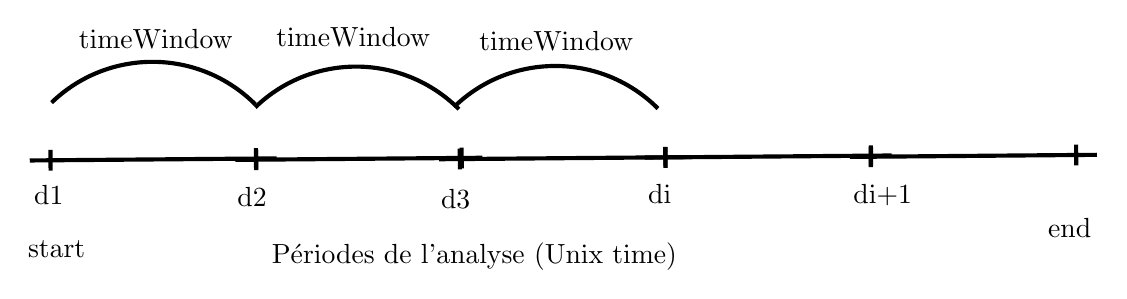
\begin{tikzpicture}[even odd rule]
\pgftransformxscale{1.000000}
\pgftransformyscale{-1.000000}
\definecolor{dialinecolor}{rgb}{0.000000, 0.000000, 0.000000}
\pgfsetstrokecolor{dialinecolor}
\pgfsetstrokeopacity{1.000000}
\definecolor{diafillcolor}{rgb}{1.000000, 1.000000, 1.000000}
\pgfsetfillcolor{diafillcolor}
\pgfsetfillopacity{1.000000}
\pgfsetlinewidth{0.100000\du}
\pgfsetdash{}{0pt}
\pgfsetbuttcap
{
\definecolor{diafillcolor}{rgb}{0.000000, 0.000000, 0.000000}
\pgfsetfillcolor{diafillcolor}
\pgfsetfillopacity{1.000000}
% was here!!!
}
\definecolor{dialinecolor}{rgb}{0.000000, 0.000000, 0.000000}
\pgfsetstrokecolor{dialinecolor}
\pgfsetstrokeopacity{1.000000}
\draw (34.600000\du,6.050000\du)--(40.550000\du,6.000000\du);
\pgfsetlinewidth{0.100000\du}
\pgfsetdash{}{0pt}
\pgfsetmiterjoin
\pgfsetbuttcap
\definecolor{dialinecolor}{rgb}{0.000000, 0.000000, 0.000000}
\pgfsetstrokecolor{dialinecolor}
\pgfsetstrokeopacity{1.000000}
\draw (35.097882\du,5.795807\du)--(35.102083\du,6.295790\du);
\pgfsetlinewidth{0.100000\du}
\pgfsetdash{}{0pt}
\pgfsetmiterjoin
\pgfsetbuttcap
\definecolor{dialinecolor}{rgb}{0.000000, 0.000000, 0.000000}
\pgfsetstrokecolor{dialinecolor}
\pgfsetstrokeopacity{1.000000}
\draw (40.052118\du,6.254193\du)--(40.047917\du,5.754210\du);
% setfont left to latex
\definecolor{dialinecolor}{rgb}{0.000000, 0.000000, 0.000000}
\pgfsetstrokecolor{dialinecolor}
\pgfsetstrokeopacity{1.000000}
\definecolor{diafillcolor}{rgb}{0.000000, 0.000000, 0.000000}
\pgfsetfillcolor{diafillcolor}
\pgfsetfillopacity{1.000000}
\node[anchor=base west,inner sep=0pt,outer sep=0pt,color=dialinecolor] at (14.800166\du,8.464650\du){start};
% setfont left to latex
\definecolor{dialinecolor}{rgb}{0.000000, 0.000000, 0.000000}
\pgfsetstrokecolor{dialinecolor}
\pgfsetstrokeopacity{1.000000}
\definecolor{diafillcolor}{rgb}{0.000000, 0.000000, 0.000000}
\pgfsetfillcolor{diafillcolor}
\pgfsetfillopacity{1.000000}
\node[anchor=base west,inner sep=0pt,outer sep=0pt,color=dialinecolor] at (39.375580\du,7.990892\du){end};
% setfont left to latex
\definecolor{dialinecolor}{rgb}{0.000000, 0.000000, 0.000000}
\pgfsetstrokecolor{dialinecolor}
\pgfsetstrokeopacity{1.000000}
\definecolor{diafillcolor}{rgb}{0.000000, 0.000000, 0.000000}
\pgfsetfillcolor{diafillcolor}
\pgfsetfillopacity{1.000000}
\node[anchor=base west,inner sep=0pt,outer sep=0pt,color=dialinecolor] at (20.674752\du,8.627312\du){Périodes de l'analyse (Unix time)};
% setfont left to latex
\definecolor{dialinecolor}{rgb}{0.000000, 0.000000, 0.000000}
\pgfsetstrokecolor{dialinecolor}
\pgfsetstrokeopacity{1.000000}
\definecolor{diafillcolor}{rgb}{0.000000, 0.000000, 0.000000}
\pgfsetfillcolor{diafillcolor}
\pgfsetfillopacity{1.000000}
\node[anchor=base west,inner sep=0pt,outer sep=0pt,color=dialinecolor] at (14.950000\du,7.200000\du){d1};
\pgfsetlinewidth{0.100000\du}
\pgfsetdash{}{0pt}
\pgfsetbuttcap
{
\definecolor{diafillcolor}{rgb}{0.000000, 0.000000, 0.000000}
\pgfsetfillcolor{diafillcolor}
\pgfsetfillopacity{1.000000}
% was here!!!
}
\definecolor{dialinecolor}{rgb}{0.000000, 0.000000, 0.000000}
\pgfsetstrokecolor{dialinecolor}
\pgfsetstrokeopacity{1.000000}
\draw (29.656799\du,6.066268\du)--(35.606799\du,6.016268\du);
\pgfsetlinewidth{0.100000\du}
\pgfsetdash{}{0pt}
\pgfsetmiterjoin
\pgfsetbuttcap
\definecolor{dialinecolor}{rgb}{0.000000, 0.000000, 0.000000}
\pgfsetstrokecolor{dialinecolor}
\pgfsetstrokeopacity{1.000000}
\draw (30.154681\du,5.812076\du)--(30.158883\du,6.312058\du);
\pgfsetlinewidth{0.100000\du}
\pgfsetdash{}{0pt}
\pgfsetmiterjoin
\pgfsetbuttcap
\definecolor{dialinecolor}{rgb}{0.000000, 0.000000, 0.000000}
\pgfsetstrokecolor{dialinecolor}
\pgfsetstrokeopacity{1.000000}
\draw (35.108918\du,6.270461\du)--(35.104716\du,5.770479\du);
\pgfsetlinewidth{0.100000\du}
\pgfsetdash{}{0pt}
\pgfsetbuttcap
{
\definecolor{diafillcolor}{rgb}{0.000000, 0.000000, 0.000000}
\pgfsetfillcolor{diafillcolor}
\pgfsetfillopacity{1.000000}
% was here!!!
}
\definecolor{dialinecolor}{rgb}{0.000000, 0.000000, 0.000000}
\pgfsetstrokecolor{dialinecolor}
\pgfsetstrokeopacity{1.000000}
\draw (24.701799\du,6.106103\du)--(30.651799\du,6.056103\du);
\pgfsetlinewidth{0.100000\du}
\pgfsetdash{}{0pt}
\pgfsetmiterjoin
\pgfsetbuttcap
\definecolor{dialinecolor}{rgb}{0.000000, 0.000000, 0.000000}
\pgfsetstrokecolor{dialinecolor}
\pgfsetstrokeopacity{1.000000}
\draw (25.199681\du,5.851910\du)--(25.203883\du,6.351892\du);
\pgfsetlinewidth{0.100000\du}
\pgfsetdash{}{0pt}
\pgfsetmiterjoin
\pgfsetbuttcap
\definecolor{dialinecolor}{rgb}{0.000000, 0.000000, 0.000000}
\pgfsetstrokecolor{dialinecolor}
\pgfsetstrokeopacity{1.000000}
\draw (30.153918\du,6.310295\du)--(30.149716\du,5.810313\du);
\pgfsetlinewidth{0.100000\du}
\pgfsetdash{}{0pt}
\pgfsetbuttcap
{
\definecolor{diafillcolor}{rgb}{0.000000, 0.000000, 0.000000}
\pgfsetfillcolor{diafillcolor}
\pgfsetfillopacity{1.000000}
% was here!!!
}
\definecolor{dialinecolor}{rgb}{0.000000, 0.000000, 0.000000}
\pgfsetstrokecolor{dialinecolor}
\pgfsetstrokeopacity{1.000000}
\draw (19.796634\du,6.121020\du)--(25.746634\du,6.071020\du);
\pgfsetlinewidth{0.100000\du}
\pgfsetdash{}{0pt}
\pgfsetmiterjoin
\pgfsetbuttcap
\definecolor{dialinecolor}{rgb}{0.000000, 0.000000, 0.000000}
\pgfsetstrokecolor{dialinecolor}
\pgfsetstrokeopacity{1.000000}
\draw (20.294515\du,5.866827\du)--(20.298717\du,6.366810\du);
\pgfsetlinewidth{0.100000\du}
\pgfsetdash{}{0pt}
\pgfsetmiterjoin
\pgfsetbuttcap
\definecolor{dialinecolor}{rgb}{0.000000, 0.000000, 0.000000}
\pgfsetstrokecolor{dialinecolor}
\pgfsetstrokeopacity{1.000000}
\draw (25.248752\du,6.325213\du)--(25.244551\du,5.825230\du);
\pgfsetlinewidth{0.100000\du}
\pgfsetdash{}{0pt}
\pgfsetbuttcap
{
\definecolor{diafillcolor}{rgb}{0.000000, 0.000000, 0.000000}
\pgfsetfillcolor{diafillcolor}
\pgfsetfillopacity{1.000000}
% was here!!!
}
\definecolor{dialinecolor}{rgb}{0.000000, 0.000000, 0.000000}
\pgfsetstrokecolor{dialinecolor}
\pgfsetstrokeopacity{1.000000}
\draw (14.841634\du,6.135937\du)--(20.791634\du,6.085937\du);
\pgfsetlinewidth{0.100000\du}
\pgfsetdash{}{0pt}
\pgfsetmiterjoin
\pgfsetbuttcap
\definecolor{dialinecolor}{rgb}{0.000000, 0.000000, 0.000000}
\pgfsetstrokecolor{dialinecolor}
\pgfsetstrokeopacity{1.000000}
\draw (15.339515\du,5.881744\du)--(15.343717\du,6.381727\du);
\pgfsetlinewidth{0.100000\du}
\pgfsetdash{}{0pt}
\pgfsetmiterjoin
\pgfsetbuttcap
\definecolor{dialinecolor}{rgb}{0.000000, 0.000000, 0.000000}
\pgfsetstrokecolor{dialinecolor}
\pgfsetstrokeopacity{1.000000}
\draw (20.293752\du,6.340130\du)--(20.289551\du,5.840147\du);
% setfont left to latex
\definecolor{dialinecolor}{rgb}{0.000000, 0.000000, 0.000000}
\pgfsetstrokecolor{dialinecolor}
\pgfsetstrokeopacity{1.000000}
\definecolor{diafillcolor}{rgb}{0.000000, 0.000000, 0.000000}
\pgfsetfillcolor{diafillcolor}
\pgfsetfillopacity{1.000000}
\node[anchor=base west,inner sep=0pt,outer sep=0pt,color=dialinecolor] at (19.845000\du,7.235000\du){d2};
% setfont left to latex
\definecolor{dialinecolor}{rgb}{0.000000, 0.000000, 0.000000}
\pgfsetstrokecolor{dialinecolor}
\pgfsetstrokeopacity{1.000000}
\definecolor{diafillcolor}{rgb}{0.000000, 0.000000, 0.000000}
\pgfsetfillcolor{diafillcolor}
\pgfsetfillopacity{1.000000}
\node[anchor=base west,inner sep=0pt,outer sep=0pt,color=dialinecolor] at (24.750000\du,7.300000\du){d3};
% setfont left to latex
\definecolor{dialinecolor}{rgb}{0.000000, 0.000000, 0.000000}
\pgfsetstrokecolor{dialinecolor}
\pgfsetstrokeopacity{1.000000}
\definecolor{diafillcolor}{rgb}{0.000000, 0.000000, 0.000000}
\pgfsetfillcolor{diafillcolor}
\pgfsetfillopacity{1.000000}
\node[anchor=base west,inner sep=0pt,outer sep=0pt,color=dialinecolor] at (29.740000\du,7.175000\du){di};
% setfont left to latex
\definecolor{dialinecolor}{rgb}{0.000000, 0.000000, 0.000000}
\pgfsetstrokecolor{dialinecolor}
\pgfsetstrokeopacity{1.000000}
\definecolor{diafillcolor}{rgb}{0.000000, 0.000000, 0.000000}
\pgfsetfillcolor{diafillcolor}
\pgfsetfillopacity{1.000000}
\node[anchor=base west,inner sep=0pt,outer sep=0pt,color=dialinecolor] at (34.685000\du,7.165000\du){di+1};
\pgfsetlinewidth{0.100000\du}
\pgfsetdash{}{0pt}
\pgfsetbuttcap
\definecolor{dialinecolor}{rgb}{0.000000, 0.000000, 0.000000}
\pgfsetstrokecolor{dialinecolor}
\pgfsetstrokeopacity{1.000000}
\pgfpathmoveto{\pgfpoint{25.180033\du}{4.900033\du}}
\pgfpatharc{315}{226}{3.501250\du and 3.501250\du}
\pgfusepath{stroke}
% setfont left to latex
\definecolor{dialinecolor}{rgb}{0.000000, 0.000000, 0.000000}
\pgfsetstrokecolor{dialinecolor}
\pgfsetstrokeopacity{1.000000}
\definecolor{diafillcolor}{rgb}{0.000000, 0.000000, 0.000000}
\pgfsetfillcolor{diafillcolor}
\pgfsetfillopacity{1.000000}
\node[anchor=base west,inner sep=0pt,outer sep=0pt,color=dialinecolor] at (20.780000\du,3.400000\du){timeWindow};
\pgfsetlinewidth{0.100000\du}
\pgfsetdash{}{0pt}
\pgfsetbuttcap
\definecolor{dialinecolor}{rgb}{0.000000, 0.000000, 0.000000}
\pgfsetstrokecolor{dialinecolor}
\pgfsetstrokeopacity{1.000000}
\pgfpathmoveto{\pgfpoint{29.975033\du}{4.885033\du}}
\pgfpatharc{315}{226}{3.501250\du and 3.501250\du}
\pgfusepath{stroke}
% setfont left to latex
\definecolor{dialinecolor}{rgb}{0.000000, 0.000000, 0.000000}
\pgfsetstrokecolor{dialinecolor}
\pgfsetstrokeopacity{1.000000}
\definecolor{diafillcolor}{rgb}{0.000000, 0.000000, 0.000000}
\pgfsetfillcolor{diafillcolor}
\pgfsetfillopacity{1.000000}
\node[anchor=base west,inner sep=0pt,outer sep=0pt,color=dialinecolor] at (25.675000\du,3.485000\du){timeWindow};
\pgfsetlinewidth{0.100000\du}
\pgfsetdash{}{0pt}
\pgfsetbuttcap
\definecolor{dialinecolor}{rgb}{0.000000, 0.000000, 0.000000}
\pgfsetstrokecolor{dialinecolor}
\pgfsetstrokeopacity{1.000000}
\pgfpathmoveto{\pgfpoint{20.275033\du}{4.785033\du}}
\pgfpatharc{315}{226}{3.501250\du and 3.501250\du}
\pgfusepath{stroke}
% setfont left to latex
\definecolor{dialinecolor}{rgb}{0.000000, 0.000000, 0.000000}
\pgfsetstrokecolor{dialinecolor}
\pgfsetstrokeopacity{1.000000}
\definecolor{diafillcolor}{rgb}{0.000000, 0.000000, 0.000000}
\pgfsetfillcolor{diafillcolor}
\pgfsetfillopacity{1.000000}
\node[anchor=base west,inner sep=0pt,outer sep=0pt,color=dialinecolor] at (16.025000\du,3.435000\du){timeWindow};
\end{tikzpicture}

	\caption{}
	\label{fig:timing_tex}
\end{figure}


Les opérations  (2 à 6) concernent  les traceroutes par tout $d_i$.  

\paragraph{2. Vérification de la validité de chaque traceroute }. Ces vérifications reprennent les points suivants:
\begin{itemize}
	\item élimination des traceroutes échoués complètement;
	\item élimination du signal contenant une adresse IP privée;
	\item élimination du signal qui ne contient pas un RTT ou celui qui contient un RTT négatif;
	\item  élimination du signal échoué.
\end{itemize}

\paragraph{3. Calcul de la médiane des RTTs par saut.} Pour tout saut d'un traceroute,  on calcul la médiane des RTTs par adresse IP. Soit le saut $h =\{s \}$ où $s$ est un  Signal, mediane\_rtt ($h$) =  $\{median(\{s.rtt\})\}$  pour tout signal $s$ ayant la même adresse IP. Autrement dit, le nouveau saut du traceroute est reconstruit en regroupant les signaux par adresse IP et ensuite en calculant leurs RTTs. 




\paragraph{4. Inférence des liens topologiques par traceroute.} Un lien topologique est formé par chaque deux routeurs consécutifs. Ce sont les deux routeurs des deux sauts consécutifs. De manière générale, la figure \ref{fig:link-inference} illustre la constitution des liens possibles  dans un traceroute. Soient  RAi, avec $i \in [1,N]$,  l'ensemble des routeurs pour le saut A et RBj, avec $j \in [1,M]$, l'ensemble  des routeurs pour le saut B, avec N et M deux entiers.



Ainsi, les liens  construits sont ceux partant de tout RAi vers tout RBj, où A et B sont deux sauts consécutifs. A l'issue de cette étape, pour tout traceroute, on obtient la liste des liens possibles tout en reprenant des informations générales de la requête traceroute.
\begin{figure}[H]
	\centering
	\captionsetup{justification=centering}
	%\includegraphics[width=0.5\linewidth]{illustrations/link-inference}
	% Graphic for TeX using PGF
% Title: /home/hayat/RipeAtlasTraceroutesAnalysis/report/illustrations/link-inference.dia
% Creator: Dia v0.97+git
% CreationDate: Thu Nov 29 20:58:09 2018
% For: hayat
% \usepackage{tikz}
% The following commands are not supported in PSTricks at present
% We define them conditionally, so when they are implemented,
% this pgf file will use them.
\ifx\du\undefined
  \newlength{\du}
\fi
\setlength{\du}{15\unitlength}
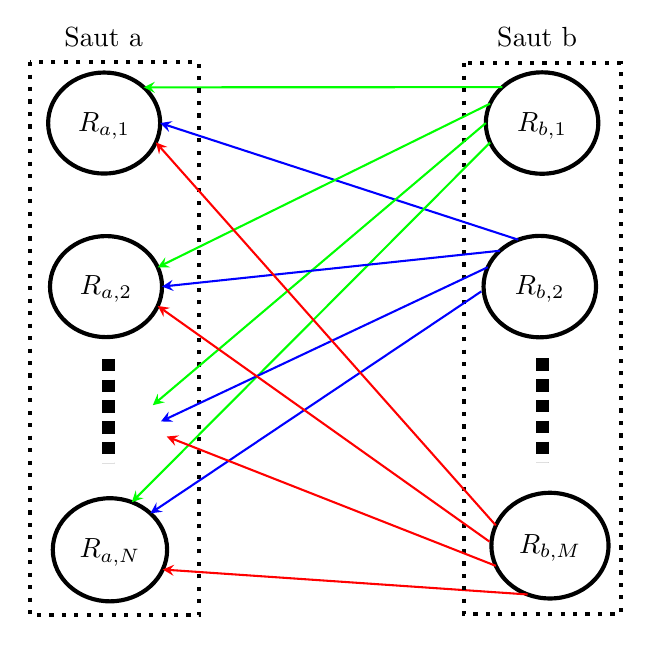
\begin{tikzpicture}[even odd rule]
\pgftransformxscale{1.000000}
\pgftransformyscale{-1.000000}
\definecolor{dialinecolor}{rgb}{0.000000, 0.000000, 0.000000}
\pgfsetstrokecolor{dialinecolor}
\pgfsetstrokeopacity{1.000000}
\definecolor{diafillcolor}{rgb}{1.000000, 1.000000, 1.000000}
\pgfsetfillcolor{diafillcolor}
\pgfsetfillopacity{1.000000}
\pgfsetlinewidth{0.100000\du}
\pgfsetdash{}{0pt}
\pgfsetmiterjoin
\definecolor{diafillcolor}{rgb}{1.000000, 1.000000, 1.000000}
\pgfsetfillcolor{diafillcolor}
\pgfsetfillopacity{1.000000}
\pgfpathellipse{\pgfpoint{27.430614\du}{13.298442\du}}{\pgfpoint{1.349214\du}{0\du}}{\pgfpoint{0\du}{1.217042\du}}
\pgfusepath{fill}
\definecolor{dialinecolor}{rgb}{0.000000, 0.000000, 0.000000}
\pgfsetstrokecolor{dialinecolor}
\pgfsetstrokeopacity{1.000000}
\pgfpathellipse{\pgfpoint{27.430614\du}{13.298442\du}}{\pgfpoint{1.349214\du}{0\du}}{\pgfpoint{0\du}{1.217042\du}}
\pgfusepath{stroke}
% setfont left to latex
\definecolor{dialinecolor}{rgb}{0.000000, 0.000000, 0.000000}
\pgfsetstrokecolor{dialinecolor}
\pgfsetstrokeopacity{1.000000}
\definecolor{diafillcolor}{rgb}{0.000000, 0.000000, 0.000000}
\pgfsetfillcolor{diafillcolor}
\pgfsetfillopacity{1.000000}
\node[anchor=base,inner sep=0pt, outer sep=0pt,color=dialinecolor] at (27.430614\du,13.493442\du){$R_{a,1}$};
\pgfsetlinewidth{0.100000\du}
\pgfsetdash{}{0pt}
\pgfsetmiterjoin
\definecolor{diafillcolor}{rgb}{1.000000, 1.000000, 1.000000}
\pgfsetfillcolor{diafillcolor}
\pgfsetfillopacity{1.000000}
\pgfpathellipse{\pgfpoint{27.475614\du}{17.238442\du}}{\pgfpoint{1.349214\du}{0\du}}{\pgfpoint{0\du}{1.217042\du}}
\pgfusepath{fill}
\definecolor{dialinecolor}{rgb}{0.000000, 0.000000, 0.000000}
\pgfsetstrokecolor{dialinecolor}
\pgfsetstrokeopacity{1.000000}
\pgfpathellipse{\pgfpoint{27.475614\du}{17.238442\du}}{\pgfpoint{1.349214\du}{0\du}}{\pgfpoint{0\du}{1.217042\du}}
\pgfusepath{stroke}
% setfont left to latex
\definecolor{dialinecolor}{rgb}{0.000000, 0.000000, 0.000000}
\pgfsetstrokecolor{dialinecolor}
\pgfsetstrokeopacity{1.000000}
\definecolor{diafillcolor}{rgb}{0.000000, 0.000000, 0.000000}
\pgfsetfillcolor{diafillcolor}
\pgfsetfillopacity{1.000000}
\node[anchor=base,inner sep=0pt, outer sep=0pt,color=dialinecolor] at (27.475614\du,17.433442\du){$R_{a,2}$};
\pgfsetlinewidth{0.100000\du}
\pgfsetdash{}{0pt}
\pgfsetmiterjoin
\definecolor{diafillcolor}{rgb}{1.000000, 1.000000, 1.000000}
\pgfsetfillcolor{diafillcolor}
\pgfsetfillopacity{1.000000}
\pgfpathellipse{\pgfpoint{27.570578\du}{23.578496\du}}{\pgfpoint{1.376878\du}{0\du}}{\pgfpoint{0\du}{1.241996\du}}
\pgfusepath{fill}
\definecolor{dialinecolor}{rgb}{0.000000, 0.000000, 0.000000}
\pgfsetstrokecolor{dialinecolor}
\pgfsetstrokeopacity{1.000000}
\pgfpathellipse{\pgfpoint{27.570578\du}{23.578496\du}}{\pgfpoint{1.376878\du}{0\du}}{\pgfpoint{0\du}{1.241996\du}}
\pgfusepath{stroke}
% setfont left to latex
\definecolor{dialinecolor}{rgb}{0.000000, 0.000000, 0.000000}
\pgfsetstrokecolor{dialinecolor}
\pgfsetstrokeopacity{1.000000}
\definecolor{diafillcolor}{rgb}{0.000000, 0.000000, 0.000000}
\pgfsetfillcolor{diafillcolor}
\pgfsetfillopacity{1.000000}
\node[anchor=base,inner sep=0pt, outer sep=0pt,color=dialinecolor] at (27.570578\du,23.773496\du){$R_{a,N}$};
\pgfsetlinewidth{0.300000\du}
\pgfsetdash{{\pgflinewidth}{0.200000\du}}{0cm}
\pgfsetbuttcap
{
\definecolor{diafillcolor}{rgb}{0.000000, 0.000000, 0.000000}
\pgfsetfillcolor{diafillcolor}
\pgfsetfillopacity{1.000000}
% was here!!!
\definecolor{dialinecolor}{rgb}{0.000000, 0.000000, 0.000000}
\pgfsetstrokecolor{dialinecolor}
\pgfsetstrokeopacity{1.000000}
\draw (27.540000\du,18.980000\du)--(27.540000\du,21.480000\du);
}
\pgfsetlinewidth{0.100000\du}
\pgfsetdash{}{0pt}
\pgfsetmiterjoin
\definecolor{diafillcolor}{rgb}{1.000000, 1.000000, 1.000000}
\pgfsetfillcolor{diafillcolor}
\pgfsetfillopacity{1.000000}
\pgfpathellipse{\pgfpoint{37.980536\du}{13.298484\du}}{\pgfpoint{1.355136\du}{0\du}}{\pgfpoint{0\du}{1.222384\du}}
\pgfusepath{fill}
\definecolor{dialinecolor}{rgb}{0.000000, 0.000000, 0.000000}
\pgfsetstrokecolor{dialinecolor}
\pgfsetstrokeopacity{1.000000}
\pgfpathellipse{\pgfpoint{37.980536\du}{13.298484\du}}{\pgfpoint{1.355136\du}{0\du}}{\pgfpoint{0\du}{1.222384\du}}
\pgfusepath{stroke}
% setfont left to latex
\definecolor{dialinecolor}{rgb}{0.000000, 0.000000, 0.000000}
\pgfsetstrokecolor{dialinecolor}
\pgfsetstrokeopacity{1.000000}
\definecolor{diafillcolor}{rgb}{0.000000, 0.000000, 0.000000}
\pgfsetfillcolor{diafillcolor}
\pgfsetfillopacity{1.000000}
\node[anchor=base,inner sep=0pt, outer sep=0pt,color=dialinecolor] at (37.980536\du,13.493484\du){$R_{b,1}$};
\pgfsetlinewidth{0.100000\du}
\pgfsetdash{}{0pt}
\pgfsetmiterjoin
\definecolor{diafillcolor}{rgb}{1.000000, 1.000000, 1.000000}
\pgfsetfillcolor{diafillcolor}
\pgfsetfillopacity{1.000000}
\pgfpathellipse{\pgfpoint{37.925536\du}{17.238484\du}}{\pgfpoint{1.355136\du}{0\du}}{\pgfpoint{0\du}{1.222384\du}}
\pgfusepath{fill}
\definecolor{dialinecolor}{rgb}{0.000000, 0.000000, 0.000000}
\pgfsetstrokecolor{dialinecolor}
\pgfsetstrokeopacity{1.000000}
\pgfpathellipse{\pgfpoint{37.925536\du}{17.238484\du}}{\pgfpoint{1.355136\du}{0\du}}{\pgfpoint{0\du}{1.222384\du}}
\pgfusepath{stroke}
% setfont left to latex
\definecolor{dialinecolor}{rgb}{0.000000, 0.000000, 0.000000}
\pgfsetstrokecolor{dialinecolor}
\pgfsetstrokeopacity{1.000000}
\definecolor{diafillcolor}{rgb}{0.000000, 0.000000, 0.000000}
\pgfsetfillcolor{diafillcolor}
\pgfsetfillopacity{1.000000}
\node[anchor=base,inner sep=0pt, outer sep=0pt,color=dialinecolor] at (37.925536\du,17.433484\du){$R_{b,2}$};
\pgfsetlinewidth{0.100000\du}
\pgfsetdash{}{0pt}
\pgfsetmiterjoin
\definecolor{diafillcolor}{rgb}{1.000000, 1.000000, 1.000000}
\pgfsetfillcolor{diafillcolor}
\pgfsetfillopacity{1.000000}
\pgfpathellipse{\pgfpoint{38.170599\du}{23.478445\du}}{\pgfpoint{1.411299\du}{0\du}}{\pgfpoint{0\du}{1.273045\du}}
\pgfusepath{fill}
\definecolor{dialinecolor}{rgb}{0.000000, 0.000000, 0.000000}
\pgfsetstrokecolor{dialinecolor}
\pgfsetstrokeopacity{1.000000}
\pgfpathellipse{\pgfpoint{38.170599\du}{23.478445\du}}{\pgfpoint{1.411299\du}{0\du}}{\pgfpoint{0\du}{1.273045\du}}
\pgfusepath{stroke}
% setfont left to latex
\definecolor{dialinecolor}{rgb}{0.000000, 0.000000, 0.000000}
\pgfsetstrokecolor{dialinecolor}
\pgfsetstrokeopacity{1.000000}
\definecolor{diafillcolor}{rgb}{0.000000, 0.000000, 0.000000}
\pgfsetfillcolor{diafillcolor}
\pgfsetfillopacity{1.000000}
\node[anchor=base,inner sep=0pt, outer sep=0pt,color=dialinecolor] at (38.170599\du,23.673445\du){$R_{b,M}$};
\pgfsetlinewidth{0.300000\du}
\pgfsetdash{{\pgflinewidth}{0.200000\du}}{0cm}
\pgfsetbuttcap
{
\definecolor{diafillcolor}{rgb}{0.000000, 0.000000, 0.000000}
\pgfsetfillcolor{diafillcolor}
\pgfsetfillopacity{1.000000}
% was here!!!
\definecolor{dialinecolor}{rgb}{0.000000, 0.000000, 0.000000}
\pgfsetstrokecolor{dialinecolor}
\pgfsetstrokeopacity{1.000000}
\draw (37.985000\du,18.970000\du)--(37.985000\du,21.470000\du);
}
\pgfsetlinewidth{0.050000\du}
\pgfsetdash{}{0pt}
\pgfsetbuttcap
{
\definecolor{diafillcolor}{rgb}{0.000000, 1.000000, 0.000000}
\pgfsetfillcolor{diafillcolor}
\pgfsetfillopacity{1.000000}
% was here!!!
\pgfsetarrowsstart{stealth}
\definecolor{dialinecolor}{rgb}{0.000000, 1.000000, 0.000000}
\pgfsetstrokecolor{dialinecolor}
\pgfsetstrokeopacity{1.000000}
\draw (28.384600\du,12.437900\du)--(37.022310\du,12.434128\du);
}
\pgfsetlinewidth{0.050000\du}
\pgfsetdash{}{0pt}
\pgfsetbuttcap
{
\definecolor{diafillcolor}{rgb}{1.000000, 0.000000, 0.000000}
\pgfsetfillcolor{diafillcolor}
\pgfsetfillopacity{1.000000}
% was here!!!
\pgfsetarrowsstart{stealth}
\definecolor{dialinecolor}{rgb}{1.000000, 0.000000, 0.000000}
\pgfsetstrokecolor{dialinecolor}
\pgfsetstrokeopacity{1.000000}
\draw (28.842600\du,24.053700\du)--(37.630518\du,24.654584\du);
}
\pgfsetlinewidth{0.100000\du}
\pgfsetdash{{\pgflinewidth}{0.200000\du}}{0cm}
\pgfsetmiterjoin
\pgfsetbuttcap
{\pgfsetcornersarced{\pgfpoint{0.000000\du}{0.000000\du}}\definecolor{dialinecolor}{rgb}{0.000000, 0.000000, 0.000000}
\pgfsetstrokecolor{dialinecolor}
\pgfsetstrokeopacity{1.000000}
\draw (25.638764\du,11.830038\du)--(25.638764\du,25.156536\du)--(29.721269\du,25.156536\du)--(29.721269\du,11.830038\du)--cycle;
}\pgfsetlinewidth{0.100000\du}
\pgfsetdash{{\pgflinewidth}{0.200000\du}}{0cm}
\pgfsetmiterjoin
\pgfsetbuttcap
{\pgfsetcornersarced{\pgfpoint{0.000000\du}{0.000000\du}}\definecolor{dialinecolor}{rgb}{0.000000, 0.000000, 0.000000}
\pgfsetstrokecolor{dialinecolor}
\pgfsetstrokeopacity{1.000000}
\draw (36.096688\du,11.857262\du)--(36.096688\du,25.128574\du)--(39.871607\du,25.128574\du)--(39.871607\du,11.857262\du)--cycle;
}% setfont left to latex
\definecolor{dialinecolor}{rgb}{0.000000, 0.000000, 0.000000}
\pgfsetstrokecolor{dialinecolor}
\pgfsetstrokeopacity{1.000000}
\definecolor{diafillcolor}{rgb}{0.000000, 0.000000, 0.000000}
\pgfsetfillcolor{diafillcolor}
\pgfsetfillopacity{1.000000}
\node[anchor=base west,inner sep=0pt,outer sep=0pt,color=dialinecolor] at (26.470600\du,11.464400\du){Saut a};
% setfont left to latex
\definecolor{dialinecolor}{rgb}{0.000000, 0.000000, 0.000000}
\pgfsetstrokecolor{dialinecolor}
\pgfsetstrokeopacity{1.000000}
\definecolor{diafillcolor}{rgb}{0.000000, 0.000000, 0.000000}
\pgfsetfillcolor{diafillcolor}
\pgfsetfillopacity{1.000000}
\node[anchor=base west,inner sep=0pt,outer sep=0pt,color=dialinecolor] at (36.898700\du,11.464100\du){Saut b};
\pgfsetlinewidth{0.050000\du}
\pgfsetdash{}{0pt}
\pgfsetbuttcap
{
\definecolor{diafillcolor}{rgb}{0.000000, 0.000000, 1.000000}
\pgfsetfillcolor{diafillcolor}
\pgfsetfillopacity{1.000000}
% was here!!!
\pgfsetarrowsstart{stealth}
\definecolor{dialinecolor}{rgb}{0.000000, 0.000000, 1.000000}
\pgfsetstrokecolor{dialinecolor}
\pgfsetstrokeopacity{1.000000}
\draw (28.779828\du,13.298442\du)--(37.406948\du,16.109148\du);
}
\pgfsetlinewidth{0.050000\du}
\pgfsetdash{}{0pt}
\pgfsetbuttcap
{
\definecolor{diafillcolor}{rgb}{0.000000, 1.000000, 0.000000}
\pgfsetfillcolor{diafillcolor}
\pgfsetfillopacity{1.000000}
% was here!!!
\pgfsetarrowsstart{stealth}
\definecolor{dialinecolor}{rgb}{0.000000, 1.000000, 0.000000}
\pgfsetstrokecolor{dialinecolor}
\pgfsetstrokeopacity{1.000000}
\draw (28.722125\du,16.772700\du)--(36.728554\du,12.830698\du);
}
\pgfsetlinewidth{0.050000\du}
\pgfsetdash{}{0pt}
\pgfsetbuttcap
{
\definecolor{diafillcolor}{rgb}{0.000000, 1.000000, 0.000000}
\pgfsetfillcolor{diafillcolor}
\pgfsetfillopacity{1.000000}
% was here!!!
\pgfsetarrowsstart{stealth}
\definecolor{dialinecolor}{rgb}{0.000000, 1.000000, 0.000000}
\pgfsetstrokecolor{dialinecolor}
\pgfsetstrokeopacity{1.000000}
\draw (28.602774\du,20.095348\du)--(36.625400\du,13.298484\du);
}
\pgfsetlinewidth{0.050000\du}
\pgfsetdash{}{0pt}
\pgfsetbuttcap
{
\definecolor{diafillcolor}{rgb}{0.000000, 1.000000, 0.000000}
\pgfsetfillcolor{diafillcolor}
\pgfsetfillopacity{1.000000}
% was here!!!
\pgfsetarrowsstart{stealth}
\definecolor{dialinecolor}{rgb}{0.000000, 1.000000, 0.000000}
\pgfsetstrokecolor{dialinecolor}
\pgfsetstrokeopacity{1.000000}
\draw (28.097487\du,22.431041\du)--(36.728554\du,13.766270\du);
}
\pgfsetlinewidth{0.050000\du}
\pgfsetdash{}{0pt}
\pgfsetbuttcap
{
\definecolor{diafillcolor}{rgb}{0.000000, 0.000000, 1.000000}
\pgfsetfillcolor{diafillcolor}
\pgfsetfillopacity{1.000000}
% was here!!!
\pgfsetarrowsstart{stealth}
\definecolor{dialinecolor}{rgb}{0.000000, 0.000000, 1.000000}
\pgfsetstrokecolor{dialinecolor}
\pgfsetstrokeopacity{1.000000}
\draw (28.824828\du,17.238442\du)--(36.967310\du,16.374128\du);
}
\pgfsetlinewidth{0.050000\du}
\pgfsetdash{}{0pt}
\pgfsetbuttcap
{
\definecolor{diafillcolor}{rgb}{0.000000, 0.000000, 1.000000}
\pgfsetfillcolor{diafillcolor}
\pgfsetfillopacity{1.000000}
% was here!!!
\pgfsetarrowsstart{stealth}
\definecolor{dialinecolor}{rgb}{0.000000, 0.000000, 1.000000}
\pgfsetstrokecolor{dialinecolor}
\pgfsetstrokeopacity{1.000000}
\draw (28.798511\du,20.486821\du)--(36.673554\du,16.770698\du);
}
\pgfsetlinewidth{0.050000\du}
\pgfsetdash{}{0pt}
\pgfsetbuttcap
{
\definecolor{diafillcolor}{rgb}{0.000000, 0.000000, 1.000000}
\pgfsetfillcolor{diafillcolor}
\pgfsetfillopacity{1.000000}
% was here!!!
\pgfsetarrowsstart{stealth}
\definecolor{dialinecolor}{rgb}{0.000000, 0.000000, 1.000000}
\pgfsetstrokecolor{dialinecolor}
\pgfsetstrokeopacity{1.000000}
\draw (28.544178\du,22.700272\du)--(36.516123\du,17.355037\du);
}
\pgfsetlinewidth{0.050000\du}
\pgfsetdash{}{0pt}
\pgfsetbuttcap
{
\definecolor{diafillcolor}{rgb}{1.000000, 0.000000, 0.000000}
\pgfsetfillcolor{diafillcolor}
\pgfsetfillopacity{1.000000}
% was here!!!
\pgfsetarrowsstart{stealth}
\definecolor{dialinecolor}{rgb}{1.000000, 0.000000, 0.000000}
\pgfsetstrokecolor{dialinecolor}
\pgfsetstrokeopacity{1.000000}
\draw (28.938323\du,20.850332\du)--(36.866729\du,23.965618\du);
}
\pgfsetlinewidth{0.050000\du}
\pgfsetdash{}{0pt}
\pgfsetbuttcap
{
\definecolor{diafillcolor}{rgb}{1.000000, 0.000000, 0.000000}
\pgfsetfillcolor{diafillcolor}
\pgfsetfillopacity{1.000000}
% was here!!!
\pgfsetarrowsstart{stealth}
\definecolor{dialinecolor}{rgb}{1.000000, 0.000000, 0.000000}
\pgfsetstrokecolor{dialinecolor}
\pgfsetstrokeopacity{1.000000}
\draw (28.722125\du,17.704183\du)--(36.712688\du,23.381227\du);
}
\pgfsetlinewidth{0.050000\du}
\pgfsetdash{}{0pt}
\pgfsetbuttcap
{
\definecolor{diafillcolor}{rgb}{1.000000, 0.000000, 0.000000}
\pgfsetfillcolor{diafillcolor}
\pgfsetfillopacity{1.000000}
% was here!!!
\pgfsetarrowsstart{stealth}
\definecolor{dialinecolor}{rgb}{1.000000, 0.000000, 0.000000}
\pgfsetstrokecolor{dialinecolor}
\pgfsetstrokeopacity{1.000000}
\draw (28.677125\du,13.764183\du)--(36.866729\du,22.991272\du);
}
\end{tikzpicture}

	\caption{Inférence des liens possibles entre les routeurs des deux sauts consécutifs RAi et RBj}
	\label{fig:link-inference}
\end{figure}
\paragraph{5. Caractérisation des liens} avec leurs RTTs différentiels. A cette étape, on calcul le RTT différentiel d'un lien en calculant la différence entre les RTTs\footnote{C'est la médiane calculée à l'étape 3.} des deux routeurs du lien en question. En plus du RTT différentiel, on note aussi la sonde Atlas ayant effectué la requête traceroute où le lien a été identifié. 

\paragraph{6. Fusion des informations d'un lien. } Etant donné qu'un lien (IP1, IP2) peut être identifié plusieurs fois pendant une même période $d_i$ d'une part, et le lien (IP2, IP1) est similaire\footnote{La similarité est mesurée par le RTT différentiel.} au lien  (IP1, IP2) d'autre part, la fusion permet de construire une nouvelle distribution des RTTs différentiels caractérisant le lien (IP1, IP2) qui reprend les RTTs différentiels du (IP1, IP2) et du (IP2, IP1).


A la fin de l'étape 6, tous les traceroutes sont analysés tout en identifiant leurs liens, et ce par $d_i$. A présent, l'objectif c'est d'identifier les dates pendant lesquelles des anomalies ont été détectées. Pour ce faire, l'idée du travail de référence c'est de conserver, pour un lien donné, une référence du RTT différentiel médian qui sera d'abord comparée avec la médiane courante du RTT différentiel et ensuite mettre à jour cette référence tout au long de la période de l'analyse.

  
  \paragraph{7. Calcul de la médiane des RTTs différentiels et   l'intervalle de confiance courant} du lien analysé. Pour un lien donné, on calcule la médiane des RTTs différentiels d'une $d_i$, ensuite on calcule les deux bornes de l'intervalle de confiance pour $d_i$.
  
  \paragraph{8. Mise à jour de la médiane et de l'intervalle de  référence du lien analysé.} La médiane des RTTs différentiels de référence sont d'abords comparés avec ceux de la période $d_i$ courante. Ensuite, ces références sont mises à jour pour prendre en compte ces nouvelles valeurs. A l'issue de cette comparaison, la liste des dates des anomalies est mise à jour.
  


\subsection{Vue globale des étapes de la détection des anomalies}
La figure 	\ref{fig:process-rttanalysis_tex} présente la succession des étapes de la détection des anomalies dans les délais d'un lien donné. 

\begin{figure}[h]
	\centering
	\resizebox{\textwidth}{\textheight}{
		% Graphic for TeX using PGF
% Title: /home/hayat/RipeAtlasTraceroutesAnalysis/dia/process-rttanalysis.dia
% Creator: Dia v0.97+git
% CreationDate: Thu Nov 29 01:56:23 2018
% For: hayat
% \usepackage{tikz}
% The following commands are not supported in PSTricks at present
% We define them conditionally, so when they are implemented,
% this pgf file will use them.
\ifx\du\undefined
  \newlength{\du}
\fi
\setlength{\du}{15\unitlength}
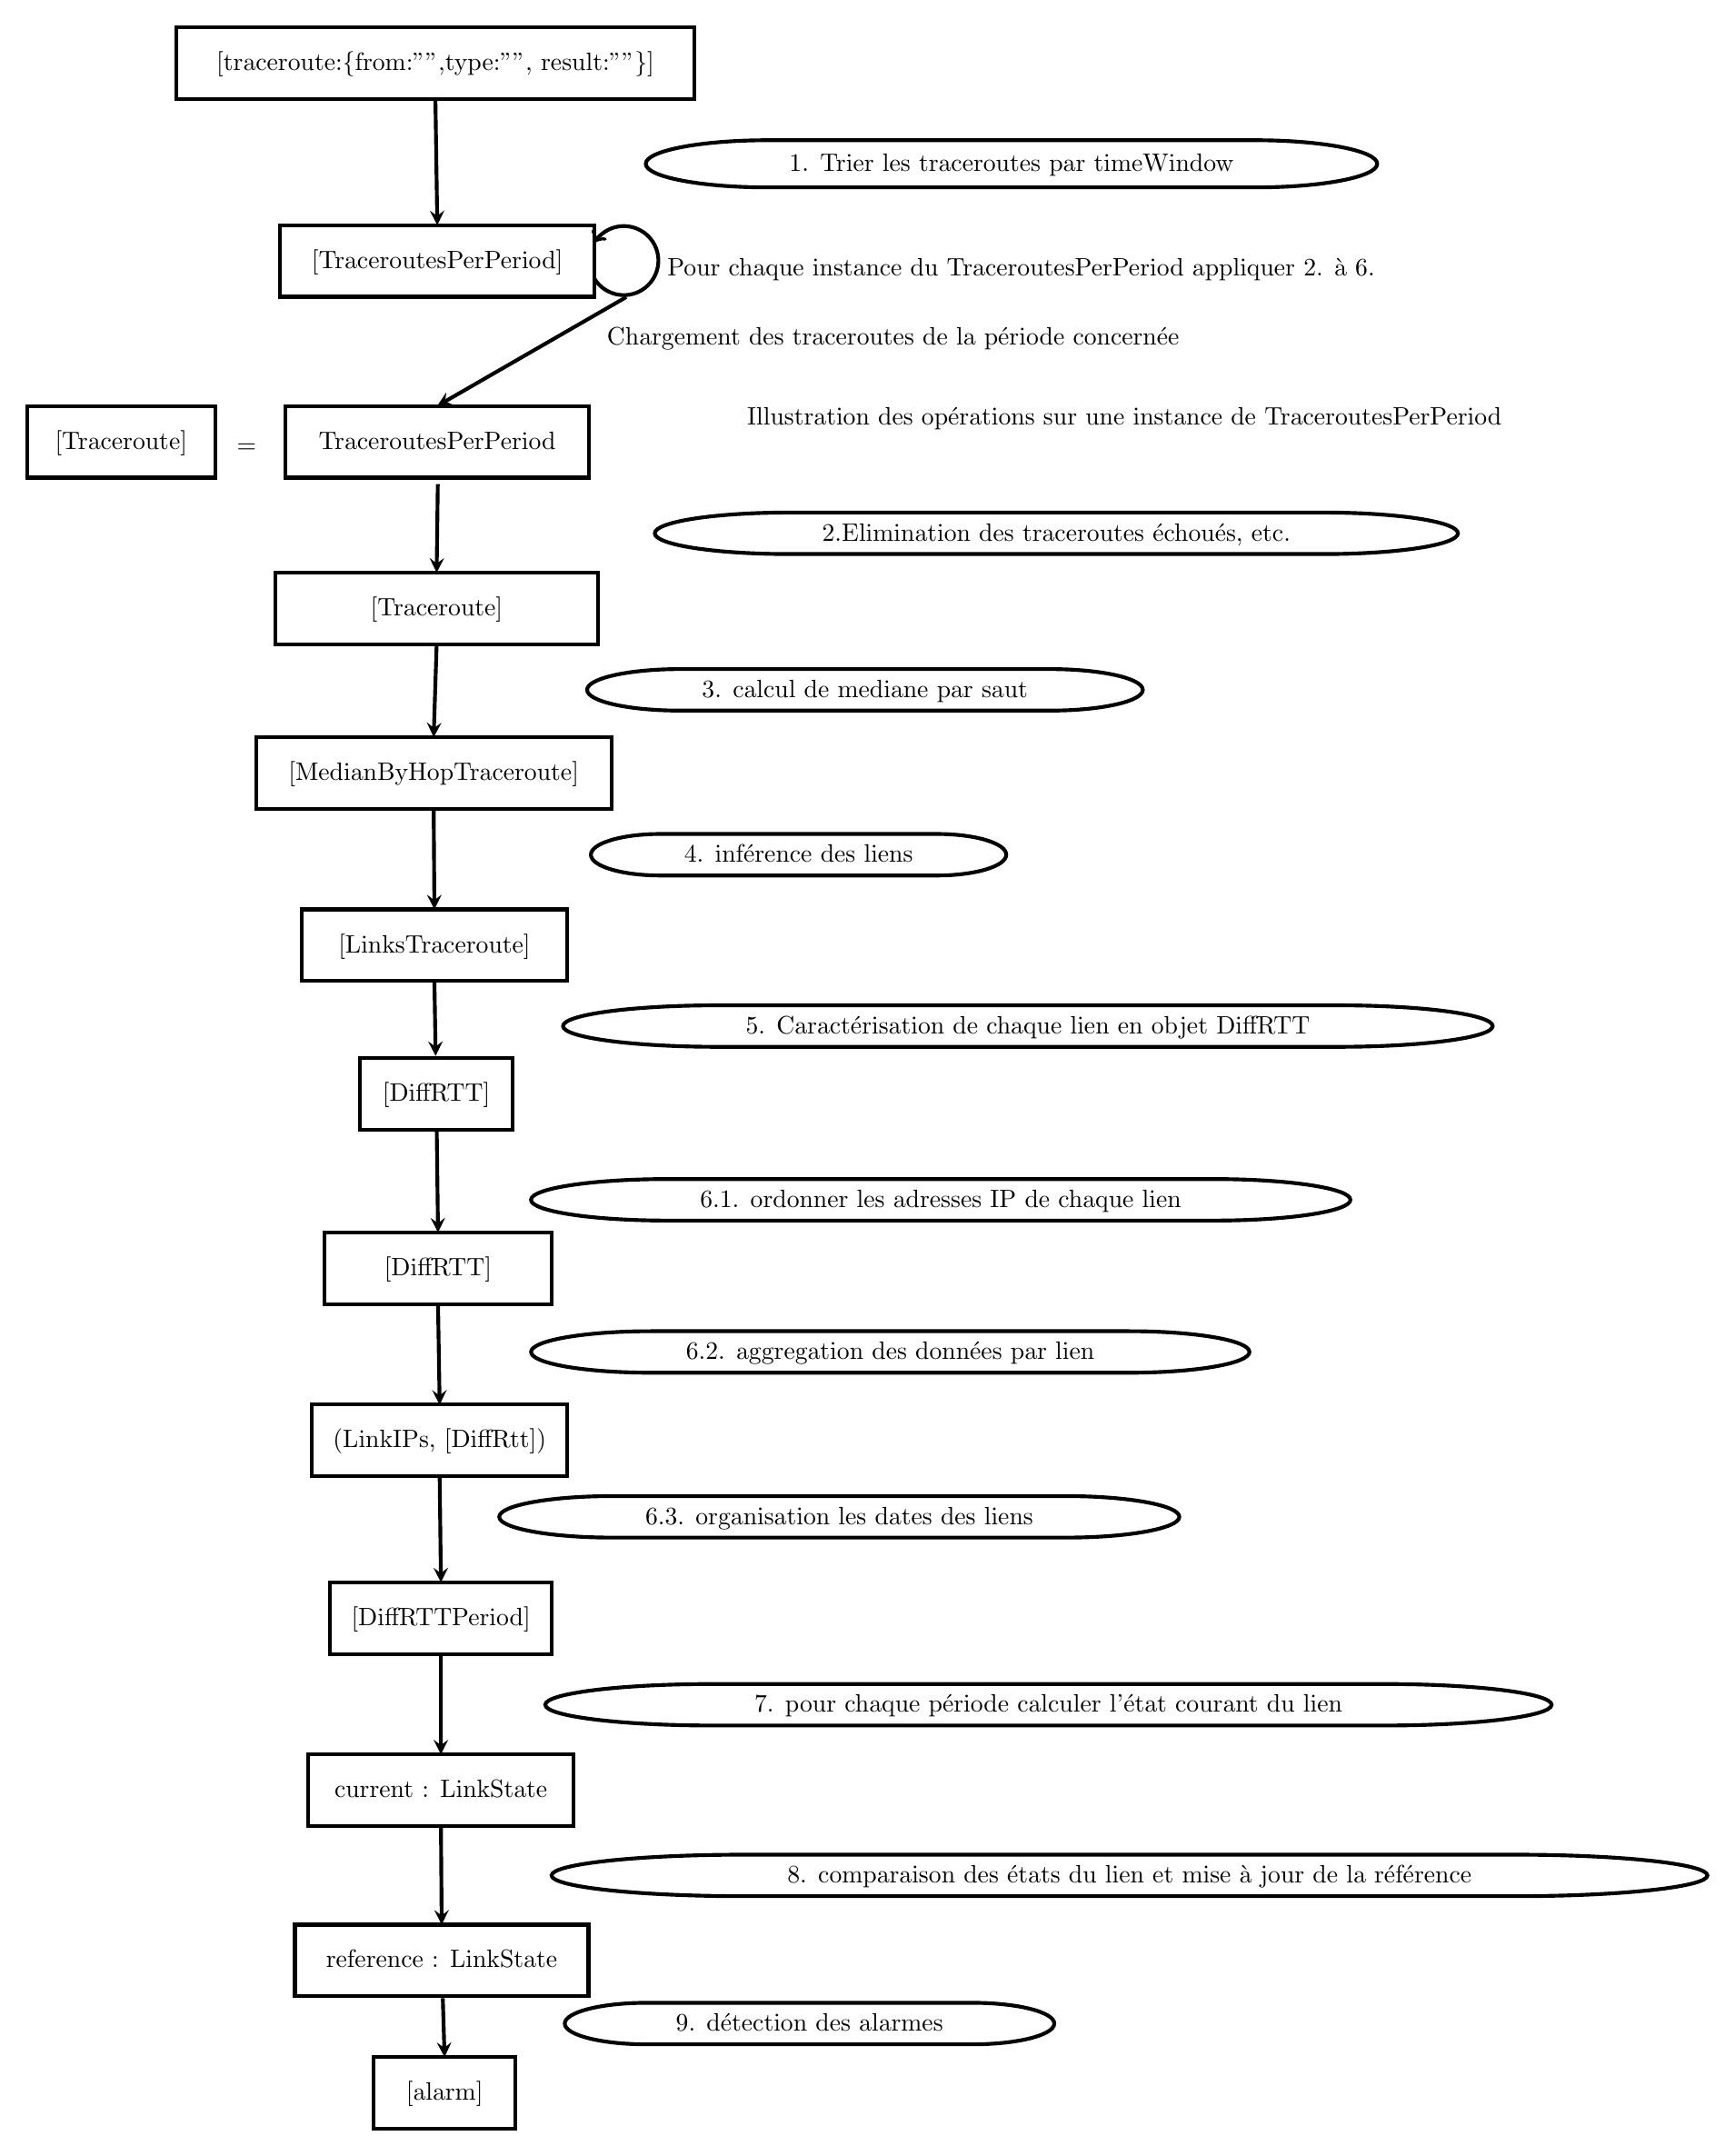
\begin{tikzpicture}[even odd rule]
\pgftransformxscale{1.000000}
\pgftransformyscale{-1.000000}
\definecolor{dialinecolor}{rgb}{0.000000, 0.000000, 0.000000}
\pgfsetstrokecolor{dialinecolor}
\pgfsetstrokeopacity{1.000000}
\definecolor{diafillcolor}{rgb}{1.000000, 1.000000, 1.000000}
\pgfsetfillcolor{diafillcolor}
\pgfsetfillopacity{1.000000}
\pgfsetlinewidth{0.100000\du}
\pgfsetdash{}{0pt}
\pgfsetmiterjoin
{\pgfsetcornersarced{\pgfpoint{0.000000\du}{0.000000\du}}\definecolor{diafillcolor}{rgb}{1.000000, 1.000000, 1.000000}
\pgfsetfillcolor{diafillcolor}
\pgfsetfillopacity{1.000000}
\fill (8.138750\du,-5.900000\du)--(8.138750\du,-4.000000\du)--(21.861250\du,-4.000000\du)--(21.861250\du,-5.900000\du)--cycle;
}{\pgfsetcornersarced{\pgfpoint{0.000000\du}{0.000000\du}}\definecolor{dialinecolor}{rgb}{0.000000, 0.000000, 0.000000}
\pgfsetstrokecolor{dialinecolor}
\pgfsetstrokeopacity{1.000000}
\draw (8.138750\du,-5.900000\du)--(8.138750\du,-4.000000\du)--(21.861250\du,-4.000000\du)--(21.861250\du,-5.900000\du)--cycle;
}% setfont left to latex
\definecolor{dialinecolor}{rgb}{0.000000, 0.000000, 0.000000}
\pgfsetstrokecolor{dialinecolor}
\pgfsetstrokeopacity{1.000000}
\definecolor{diafillcolor}{rgb}{0.000000, 0.000000, 0.000000}
\pgfsetfillcolor{diafillcolor}
\pgfsetfillopacity{1.000000}
\node[anchor=base,inner sep=0pt, outer sep=0pt,color=dialinecolor] at (15.000000\du,-4.755000\du){\ensuremath{[}traceroute:\{from:"",type:"", result:""\}\ensuremath{]}};
\pgfsetlinewidth{0.100000\du}
\pgfsetdash{}{0pt}
\pgfsetbuttcap
{
\definecolor{diafillcolor}{rgb}{0.000000, 0.000000, 0.000000}
\pgfsetfillcolor{diafillcolor}
\pgfsetfillopacity{1.000000}
% was here!!!
\pgfsetarrowsend{stealth}
\definecolor{dialinecolor}{rgb}{0.000000, 0.000000, 0.000000}
\pgfsetstrokecolor{dialinecolor}
\pgfsetstrokeopacity{1.000000}
\draw (20.060900\du,1.256430\du)--(15.048400\du,4.142720\du);
}
\pgfsetlinewidth{0.100000\du}
\pgfsetdash{}{0pt}
\pgfsetmiterjoin
{\pgfsetcornersarced{\pgfpoint{0.000000\du}{0.000000\du}}\definecolor{diafillcolor}{rgb}{1.000000, 1.000000, 1.000000}
\pgfsetfillcolor{diafillcolor}
\pgfsetfillopacity{1.000000}
\fill (4.175940\du,4.142080\du)--(4.175940\du,6.042080\du)--(9.163440\du,6.042080\du)--(9.163440\du,4.142080\du)--cycle;
}{\pgfsetcornersarced{\pgfpoint{0.000000\du}{0.000000\du}}\definecolor{dialinecolor}{rgb}{0.000000, 0.000000, 0.000000}
\pgfsetstrokecolor{dialinecolor}
\pgfsetstrokeopacity{1.000000}
\draw (4.175940\du,4.142080\du)--(4.175940\du,6.042080\du)--(9.163440\du,6.042080\du)--(9.163440\du,4.142080\du)--cycle;
}% setfont left to latex
\definecolor{dialinecolor}{rgb}{0.000000, 0.000000, 0.000000}
\pgfsetstrokecolor{dialinecolor}
\pgfsetstrokeopacity{1.000000}
\definecolor{diafillcolor}{rgb}{0.000000, 0.000000, 0.000000}
\pgfsetfillcolor{diafillcolor}
\pgfsetfillopacity{1.000000}
\node[anchor=base,inner sep=0pt, outer sep=0pt,color=dialinecolor] at (6.669690\du,5.287080\du){\ensuremath{[}Traceroute\ensuremath{]}};
% setfont left to latex
\definecolor{dialinecolor}{rgb}{0.000000, 0.000000, 0.000000}
\pgfsetstrokecolor{dialinecolor}
\pgfsetstrokeopacity{1.000000}
\definecolor{diafillcolor}{rgb}{0.000000, 0.000000, 0.000000}
\pgfsetfillcolor{diafillcolor}
\pgfsetfillopacity{1.000000}
\node[anchor=base west,inner sep=0pt,outer sep=0pt,color=dialinecolor] at (16.400000\du,9.562040\du){};
\pgfsetlinewidth{0.100000\du}
\pgfsetdash{}{0pt}
\pgfsetbuttcap
\pgfsetmiterjoin
\pgfsetlinewidth{0.100000\du}
\pgfsetbuttcap
\pgfsetmiterjoin
\pgfsetdash{}{0pt}
\definecolor{diafillcolor}{rgb}{1.000000, 1.000000, 1.000000}
\pgfsetfillcolor{diafillcolor}
\pgfsetfillopacity{1.000000}
\definecolor{dialinecolor}{rgb}{0.000000, 0.000000, 0.000000}
\pgfsetstrokecolor{dialinecolor}
\pgfsetstrokeopacity{1.000000}
\pgfpathmoveto{\pgfpoint{24.362725\du}{6.967570\du}}
\pgfpathlineto{\pgfpoint{38.555225\du}{6.967570\du}}
\pgfpathcurveto{\pgfpoint{40.514801\du}{6.967570\du}}{\pgfpoint{42.103350\du}{7.213813\du}}{\pgfpoint{42.103350\du}{7.517570\du}}
\pgfpathcurveto{\pgfpoint{42.103350\du}{7.821327\du}}{\pgfpoint{40.514801\du}{8.067570\du}}{\pgfpoint{38.555225\du}{8.067570\du}}
\pgfpathlineto{\pgfpoint{24.362725\du}{8.067570\du}}
\pgfpathcurveto{\pgfpoint{22.403149\du}{8.067570\du}}{\pgfpoint{20.814600\du}{7.821327\du}}{\pgfpoint{20.814600\du}{7.517570\du}}
\pgfpathcurveto{\pgfpoint{20.814600\du}{7.213813\du}}{\pgfpoint{22.403149\du}{6.967570\du}}{\pgfpoint{24.362725\du}{6.967570\du}}
\pgfpathclose
\pgfusepath{fill,stroke}
% setfont left to latex
\definecolor{dialinecolor}{rgb}{0.000000, 0.000000, 0.000000}
\pgfsetstrokecolor{dialinecolor}
\pgfsetstrokeopacity{1.000000}
\definecolor{diafillcolor}{rgb}{0.000000, 0.000000, 0.000000}
\pgfsetfillcolor{diafillcolor}
\pgfsetfillopacity{1.000000}
\node[anchor=base,inner sep=0pt, outer sep=0pt,color=dialinecolor] at (31.458975\du,7.717570\du){2.Elimination des traceroutes échoués, etc.};
\pgfsetlinewidth{0.100000\du}
\pgfsetdash{}{0pt}
\pgfsetmiterjoin
{\pgfsetcornersarced{\pgfpoint{0.000000\du}{0.000000\du}}\definecolor{diafillcolor}{rgb}{1.000000, 1.000000, 1.000000}
\pgfsetfillcolor{diafillcolor}
\pgfsetfillopacity{1.000000}
\fill (10.748200\du,8.560140\du)--(10.748200\du,10.460140\du)--(19.318200\du,10.460140\du)--(19.318200\du,8.560140\du)--cycle;
}{\pgfsetcornersarced{\pgfpoint{0.000000\du}{0.000000\du}}\definecolor{dialinecolor}{rgb}{0.000000, 0.000000, 0.000000}
\pgfsetstrokecolor{dialinecolor}
\pgfsetstrokeopacity{1.000000}
\draw (10.748200\du,8.560140\du)--(10.748200\du,10.460140\du)--(19.318200\du,10.460140\du)--(19.318200\du,8.560140\du)--cycle;
}% setfont left to latex
\definecolor{dialinecolor}{rgb}{0.000000, 0.000000, 0.000000}
\pgfsetstrokecolor{dialinecolor}
\pgfsetstrokeopacity{1.000000}
\definecolor{diafillcolor}{rgb}{0.000000, 0.000000, 0.000000}
\pgfsetfillcolor{diafillcolor}
\pgfsetfillopacity{1.000000}
\node[anchor=base,inner sep=0pt, outer sep=0pt,color=dialinecolor] at (15.033200\du,9.705140\du){\ensuremath{[}Traceroute\ensuremath{]}};
\pgfsetlinewidth{0.100000\du}
\pgfsetdash{}{0pt}
\pgfsetbuttcap
{
\definecolor{diafillcolor}{rgb}{0.000000, 0.000000, 0.000000}
\pgfsetfillcolor{diafillcolor}
\pgfsetfillopacity{1.000000}
% was here!!!
\pgfsetarrowsend{stealth}
\definecolor{dialinecolor}{rgb}{0.000000, 0.000000, 0.000000}
\pgfsetstrokecolor{dialinecolor}
\pgfsetstrokeopacity{1.000000}
\draw (15.063300\du,6.216320\du)--(15.033200\du,8.560140\du);
}
\pgfsetlinewidth{0.100000\du}
\pgfsetdash{}{0pt}
\pgfsetmiterjoin
{\pgfsetcornersarced{\pgfpoint{0.000000\du}{0.000000\du}}\definecolor{diafillcolor}{rgb}{1.000000, 1.000000, 1.000000}
\pgfsetfillcolor{diafillcolor}
\pgfsetfillopacity{1.000000}
\fill (11.463400\du,17.484800\du)--(11.463400\du,19.384800\du)--(18.483400\du,19.384800\du)--(18.483400\du,17.484800\du)--cycle;
}{\pgfsetcornersarced{\pgfpoint{0.000000\du}{0.000000\du}}\definecolor{dialinecolor}{rgb}{0.000000, 0.000000, 0.000000}
\pgfsetstrokecolor{dialinecolor}
\pgfsetstrokeopacity{1.000000}
\draw (11.463400\du,17.484800\du)--(11.463400\du,19.384800\du)--(18.483400\du,19.384800\du)--(18.483400\du,17.484800\du)--cycle;
}% setfont left to latex
\definecolor{dialinecolor}{rgb}{0.000000, 0.000000, 0.000000}
\pgfsetstrokecolor{dialinecolor}
\pgfsetstrokeopacity{1.000000}
\definecolor{diafillcolor}{rgb}{0.000000, 0.000000, 0.000000}
\pgfsetfillcolor{diafillcolor}
\pgfsetfillopacity{1.000000}
\node[anchor=base,inner sep=0pt, outer sep=0pt,color=dialinecolor] at (14.973400\du,18.629800\du){\ensuremath{[}LinksTraceroute\ensuremath{]}};
\pgfsetlinewidth{0.100000\du}
\pgfsetdash{}{0pt}
\pgfsetbuttcap
{
\definecolor{diafillcolor}{rgb}{0.000000, 0.000000, 0.000000}
\pgfsetfillcolor{diafillcolor}
\pgfsetfillopacity{1.000000}
% was here!!!
\pgfsetarrowsend{stealth}
\definecolor{dialinecolor}{rgb}{0.000000, 0.000000, 0.000000}
\pgfsetstrokecolor{dialinecolor}
\pgfsetstrokeopacity{1.000000}
\draw (14.954000\du,14.821200\du)--(14.973400\du,17.484800\du);
}
\pgfsetlinewidth{0.100000\du}
\pgfsetdash{}{0pt}
\pgfsetbuttcap
{
\definecolor{diafillcolor}{rgb}{0.000000, 0.000000, 0.000000}
\pgfsetfillcolor{diafillcolor}
\pgfsetfillopacity{1.000000}
% was here!!!
\pgfsetarrowsend{stealth}
\definecolor{dialinecolor}{rgb}{0.000000, 0.000000, 0.000000}
\pgfsetstrokecolor{dialinecolor}
\pgfsetstrokeopacity{1.000000}
\draw (15.033200\du,10.460100\du)--(14.954000\du,12.921200\du);
}
\pgfsetlinewidth{0.100000\du}
\pgfsetdash{}{0pt}
\pgfsetmiterjoin
{\pgfsetcornersarced{\pgfpoint{0.000000\du}{0.000000\du}}\definecolor{diafillcolor}{rgb}{1.000000, 1.000000, 1.000000}
\pgfsetfillcolor{diafillcolor}
\pgfsetfillopacity{1.000000}
\fill (10.244000\du,12.921200\du)--(10.244000\du,14.821200\du)--(19.664000\du,14.821200\du)--(19.664000\du,12.921200\du)--cycle;
}{\pgfsetcornersarced{\pgfpoint{0.000000\du}{0.000000\du}}\definecolor{dialinecolor}{rgb}{0.000000, 0.000000, 0.000000}
\pgfsetstrokecolor{dialinecolor}
\pgfsetstrokeopacity{1.000000}
\draw (10.244000\du,12.921200\du)--(10.244000\du,14.821200\du)--(19.664000\du,14.821200\du)--(19.664000\du,12.921200\du)--cycle;
}% setfont left to latex
\definecolor{dialinecolor}{rgb}{0.000000, 0.000000, 0.000000}
\pgfsetstrokecolor{dialinecolor}
\pgfsetstrokeopacity{1.000000}
\definecolor{diafillcolor}{rgb}{0.000000, 0.000000, 0.000000}
\pgfsetfillcolor{diafillcolor}
\pgfsetfillopacity{1.000000}
\node[anchor=base,inner sep=0pt, outer sep=0pt,color=dialinecolor] at (14.954000\du,14.066200\du){\ensuremath{[}MedianByHopTraceroute\ensuremath{]}};
\pgfsetlinewidth{0.100000\du}
\pgfsetdash{}{0pt}
\pgfsetbuttcap
\pgfsetmiterjoin
\pgfsetlinewidth{0.100000\du}
\pgfsetbuttcap
\pgfsetmiterjoin
\pgfsetdash{}{0pt}
\definecolor{diafillcolor}{rgb}{1.000000, 1.000000, 1.000000}
\pgfsetfillcolor{diafillcolor}
\pgfsetfillopacity{1.000000}
\definecolor{dialinecolor}{rgb}{0.000000, 0.000000, 0.000000}
\pgfsetstrokecolor{dialinecolor}
\pgfsetstrokeopacity{1.000000}
\pgfpathmoveto{\pgfpoint{21.475800\du}{11.116500\du}}
\pgfpathlineto{\pgfpoint{31.295800\du}{11.116500\du}}
\pgfpathcurveto{\pgfpoint{32.651660\du}{11.116500\du}}{\pgfpoint{33.750800\du}{11.362743\du}}{\pgfpoint{33.750800\du}{11.666500\du}}
\pgfpathcurveto{\pgfpoint{33.750800\du}{11.970257\du}}{\pgfpoint{32.651660\du}{12.216500\du}}{\pgfpoint{31.295800\du}{12.216500\du}}
\pgfpathlineto{\pgfpoint{21.475800\du}{12.216500\du}}
\pgfpathcurveto{\pgfpoint{20.119940\du}{12.216500\du}}{\pgfpoint{19.020800\du}{11.970257\du}}{\pgfpoint{19.020800\du}{11.666500\du}}
\pgfpathcurveto{\pgfpoint{19.020800\du}{11.362743\du}}{\pgfpoint{20.119940\du}{11.116500\du}}{\pgfpoint{21.475800\du}{11.116500\du}}
\pgfpathclose
\pgfusepath{fill,stroke}
% setfont left to latex
\definecolor{dialinecolor}{rgb}{0.000000, 0.000000, 0.000000}
\pgfsetstrokecolor{dialinecolor}
\pgfsetstrokeopacity{1.000000}
\definecolor{diafillcolor}{rgb}{0.000000, 0.000000, 0.000000}
\pgfsetfillcolor{diafillcolor}
\pgfsetfillopacity{1.000000}
\node[anchor=base,inner sep=0pt, outer sep=0pt,color=dialinecolor] at (26.385800\du,11.866500\du){3. calcul de mediane par saut};
\pgfsetlinewidth{0.100000\du}
\pgfsetdash{}{0pt}
\pgfsetbuttcap
\pgfsetmiterjoin
\pgfsetlinewidth{0.100000\du}
\pgfsetbuttcap
\pgfsetmiterjoin
\pgfsetdash{}{0pt}
\definecolor{diafillcolor}{rgb}{1.000000, 1.000000, 1.000000}
\pgfsetfillcolor{diafillcolor}
\pgfsetfillopacity{1.000000}
\definecolor{dialinecolor}{rgb}{0.000000, 0.000000, 0.000000}
\pgfsetstrokecolor{dialinecolor}
\pgfsetstrokeopacity{1.000000}
\pgfpathmoveto{\pgfpoint{20.956000\du}{15.486500\du}}
\pgfpathlineto{\pgfpoint{28.296000\du}{15.486500\du}}
\pgfpathcurveto{\pgfpoint{29.309443\du}{15.486500\du}}{\pgfpoint{30.131000\du}{15.732743\du}}{\pgfpoint{30.131000\du}{16.036500\du}}
\pgfpathcurveto{\pgfpoint{30.131000\du}{16.340257\du}}{\pgfpoint{29.309443\du}{16.586500\du}}{\pgfpoint{28.296000\du}{16.586500\du}}
\pgfpathlineto{\pgfpoint{20.956000\du}{16.586500\du}}
\pgfpathcurveto{\pgfpoint{19.942557\du}{16.586500\du}}{\pgfpoint{19.121000\du}{16.340257\du}}{\pgfpoint{19.121000\du}{16.036500\du}}
\pgfpathcurveto{\pgfpoint{19.121000\du}{15.732743\du}}{\pgfpoint{19.942557\du}{15.486500\du}}{\pgfpoint{20.956000\du}{15.486500\du}}
\pgfpathclose
\pgfusepath{fill,stroke}
% setfont left to latex
\definecolor{dialinecolor}{rgb}{0.000000, 0.000000, 0.000000}
\pgfsetstrokecolor{dialinecolor}
\pgfsetstrokeopacity{1.000000}
\definecolor{diafillcolor}{rgb}{0.000000, 0.000000, 0.000000}
\pgfsetfillcolor{diafillcolor}
\pgfsetfillopacity{1.000000}
\node[anchor=base,inner sep=0pt, outer sep=0pt,color=dialinecolor] at (24.626000\du,16.236500\du){4. inférence des liens };
\pgfsetlinewidth{0.100000\du}
\pgfsetdash{}{0pt}
\pgfsetmiterjoin
{\pgfsetcornersarced{\pgfpoint{0.000000\du}{0.000000\du}}\definecolor{diafillcolor}{rgb}{1.000000, 1.000000, 1.000000}
\pgfsetfillcolor{diafillcolor}
\pgfsetfillopacity{1.000000}
\fill (13.005900\du,21.418700\du)--(13.005900\du,23.318700\du)--(17.040900\du,23.318700\du)--(17.040900\du,21.418700\du)--cycle;
}{\pgfsetcornersarced{\pgfpoint{0.000000\du}{0.000000\du}}\definecolor{dialinecolor}{rgb}{0.000000, 0.000000, 0.000000}
\pgfsetstrokecolor{dialinecolor}
\pgfsetstrokeopacity{1.000000}
\draw (13.005900\du,21.418700\du)--(13.005900\du,23.318700\du)--(17.040900\du,23.318700\du)--(17.040900\du,21.418700\du)--cycle;
}% setfont left to latex
\definecolor{dialinecolor}{rgb}{0.000000, 0.000000, 0.000000}
\pgfsetstrokecolor{dialinecolor}
\pgfsetstrokeopacity{1.000000}
\definecolor{diafillcolor}{rgb}{0.000000, 0.000000, 0.000000}
\pgfsetfillcolor{diafillcolor}
\pgfsetfillopacity{1.000000}
\node[anchor=base,inner sep=0pt, outer sep=0pt,color=dialinecolor] at (15.023400\du,22.563700\du){\ensuremath{[}DiffRTT\ensuremath{]}};
\pgfsetlinewidth{0.100000\du}
\pgfsetdash{}{0pt}
\pgfsetbuttcap
{
\definecolor{diafillcolor}{rgb}{0.000000, 0.000000, 0.000000}
\pgfsetfillcolor{diafillcolor}
\pgfsetfillopacity{1.000000}
% was here!!!
\pgfsetarrowsend{stealth}
\definecolor{dialinecolor}{rgb}{0.000000, 0.000000, 0.000000}
\pgfsetstrokecolor{dialinecolor}
\pgfsetstrokeopacity{1.000000}
\draw (14.973400\du,19.384800\du)--(15.006640\du,21.368482\du);
}
\pgfsetlinewidth{0.100000\du}
\pgfsetdash{}{0pt}
\pgfsetbuttcap
\pgfsetmiterjoin
\pgfsetlinewidth{0.100000\du}
\pgfsetbuttcap
\pgfsetmiterjoin
\pgfsetdash{}{0pt}
\definecolor{diafillcolor}{rgb}{1.000000, 1.000000, 1.000000}
\pgfsetfillcolor{diafillcolor}
\pgfsetfillopacity{1.000000}
\definecolor{dialinecolor}{rgb}{0.000000, 0.000000, 0.000000}
\pgfsetstrokecolor{dialinecolor}
\pgfsetstrokeopacity{1.000000}
\pgfpathmoveto{\pgfpoint{22.489775\du}{20.027600\du}}
\pgfpathlineto{\pgfpoint{38.917275\du}{20.027600\du}}
\pgfpathcurveto{\pgfpoint{41.185440\du}{20.027600\du}}{\pgfpoint{43.024150\du}{20.273843\du}}{\pgfpoint{43.024150\du}{20.577600\du}}
\pgfpathcurveto{\pgfpoint{43.024150\du}{20.881357\du}}{\pgfpoint{41.185440\du}{21.127600\du}}{\pgfpoint{38.917275\du}{21.127600\du}}
\pgfpathlineto{\pgfpoint{22.489775\du}{21.127600\du}}
\pgfpathcurveto{\pgfpoint{20.221610\du}{21.127600\du}}{\pgfpoint{18.382900\du}{20.881357\du}}{\pgfpoint{18.382900\du}{20.577600\du}}
\pgfpathcurveto{\pgfpoint{18.382900\du}{20.273843\du}}{\pgfpoint{20.221610\du}{20.027600\du}}{\pgfpoint{22.489775\du}{20.027600\du}}
\pgfpathclose
\pgfusepath{fill,stroke}
% setfont left to latex
\definecolor{dialinecolor}{rgb}{0.000000, 0.000000, 0.000000}
\pgfsetstrokecolor{dialinecolor}
\pgfsetstrokeopacity{1.000000}
\definecolor{diafillcolor}{rgb}{0.000000, 0.000000, 0.000000}
\pgfsetfillcolor{diafillcolor}
\pgfsetfillopacity{1.000000}
\node[anchor=base,inner sep=0pt, outer sep=0pt,color=dialinecolor] at (30.703525\du,20.777600\du){5. Caractérisation de chaque lien en objet DiffRTT };
\pgfsetlinewidth{0.100000\du}
\pgfsetdash{}{0pt}
\pgfsetbuttcap
{
\definecolor{diafillcolor}{rgb}{0.000000, 0.000000, 0.000000}
\pgfsetfillcolor{diafillcolor}
\pgfsetfillopacity{1.000000}
% was here!!!
\pgfsetarrowsend{stealth}
\definecolor{dialinecolor}{rgb}{0.000000, 0.000000, 0.000000}
\pgfsetstrokecolor{dialinecolor}
\pgfsetstrokeopacity{1.000000}
\draw (15.035872\du,23.368063\du)--(15.069300\du,26.046500\du);
}
\pgfsetlinewidth{0.100000\du}
\pgfsetdash{}{0pt}
\pgfsetmiterjoin
{\pgfsetcornersarced{\pgfpoint{0.000000\du}{0.000000\du}}\definecolor{diafillcolor}{rgb}{1.000000, 1.000000, 1.000000}
\pgfsetfillcolor{diafillcolor}
\pgfsetfillopacity{1.000000}
\fill (10.881300\du,-0.650000\du)--(10.881300\du,1.250000\du)--(19.218800\du,1.250000\du)--(19.218800\du,-0.650000\du)--cycle;
}{\pgfsetcornersarced{\pgfpoint{0.000000\du}{0.000000\du}}\definecolor{dialinecolor}{rgb}{0.000000, 0.000000, 0.000000}
\pgfsetstrokecolor{dialinecolor}
\pgfsetstrokeopacity{1.000000}
\draw (10.881300\du,-0.650000\du)--(10.881300\du,1.250000\du)--(19.218800\du,1.250000\du)--(19.218800\du,-0.650000\du)--cycle;
}% setfont left to latex
\definecolor{dialinecolor}{rgb}{0.000000, 0.000000, 0.000000}
\pgfsetstrokecolor{dialinecolor}
\pgfsetstrokeopacity{1.000000}
\definecolor{diafillcolor}{rgb}{0.000000, 0.000000, 0.000000}
\pgfsetfillcolor{diafillcolor}
\pgfsetfillopacity{1.000000}
\node[anchor=base,inner sep=0pt, outer sep=0pt,color=dialinecolor] at (15.050050\du,0.495000\du){\ensuremath{[}TraceroutesPerPeriod\ensuremath{]}};
\pgfsetlinewidth{0.100000\du}
\pgfsetdash{}{0pt}
\pgfsetbuttcap
{
\definecolor{diafillcolor}{rgb}{0.000000, 0.000000, 0.000000}
\pgfsetfillcolor{diafillcolor}
\pgfsetfillopacity{1.000000}
% was here!!!
\pgfsetarrowsend{stealth}
\definecolor{dialinecolor}{rgb}{0.000000, 0.000000, 0.000000}
\pgfsetstrokecolor{dialinecolor}
\pgfsetstrokeopacity{1.000000}
\draw (15.000000\du,-4.000000\du)--(15.050100\du,-0.650000\du);
}
\pgfsetlinewidth{0.100000\du}
\pgfsetdash{}{0pt}
\pgfsetbuttcap
\pgfsetmiterjoin
\pgfsetlinewidth{0.100000\du}
\pgfsetbuttcap
\pgfsetmiterjoin
\pgfsetdash{}{0pt}
\definecolor{diafillcolor}{rgb}{1.000000, 1.000000, 1.000000}
\pgfsetfillcolor{diafillcolor}
\pgfsetfillopacity{1.000000}
\definecolor{dialinecolor}{rgb}{0.000000, 0.000000, 0.000000}
\pgfsetstrokecolor{dialinecolor}
\pgfsetstrokeopacity{1.000000}
\pgfpathmoveto{\pgfpoint{23.806850\du}{-2.900000\du}}
\pgfpathlineto{\pgfpoint{36.731850\du}{-2.900000\du}}
\pgfpathcurveto{\pgfpoint{38.516421\du}{-2.900000\du}}{\pgfpoint{39.963100\du}{-2.620178\du}}{\pgfpoint{39.963100\du}{-2.275000\du}}
\pgfpathcurveto{\pgfpoint{39.963100\du}{-1.929822\du}}{\pgfpoint{38.516421\du}{-1.650000\du}}{\pgfpoint{36.731850\du}{-1.650000\du}}
\pgfpathlineto{\pgfpoint{23.806850\du}{-1.650000\du}}
\pgfpathcurveto{\pgfpoint{22.022279\du}{-1.650000\du}}{\pgfpoint{20.575600\du}{-1.929822\du}}{\pgfpoint{20.575600\du}{-2.275000\du}}
\pgfpathcurveto{\pgfpoint{20.575600\du}{-2.620178\du}}{\pgfpoint{22.022279\du}{-2.900000\du}}{\pgfpoint{23.806850\du}{-2.900000\du}}
\pgfpathclose
\pgfusepath{fill,stroke}
% setfont left to latex
\definecolor{dialinecolor}{rgb}{0.000000, 0.000000, 0.000000}
\pgfsetstrokecolor{dialinecolor}
\pgfsetstrokeopacity{1.000000}
\definecolor{diafillcolor}{rgb}{0.000000, 0.000000, 0.000000}
\pgfsetfillcolor{diafillcolor}
\pgfsetfillopacity{1.000000}
\node[anchor=base,inner sep=0pt, outer sep=0pt,color=dialinecolor] at (30.269350\du,-2.075000\du){1. Trier les traceroutes par timeWindow};
% setfont left to latex
\definecolor{dialinecolor}{rgb}{0.000000, 0.000000, 0.000000}
\pgfsetstrokecolor{dialinecolor}
\pgfsetstrokeopacity{1.000000}
\definecolor{diafillcolor}{rgb}{0.000000, 0.000000, 0.000000}
\pgfsetfillcolor{diafillcolor}
\pgfsetfillopacity{1.000000}
\node[anchor=base west,inner sep=0pt,outer sep=0pt,color=dialinecolor] at (21.150000\du,0.700000\du){ Pour chaque instance du TraceroutesPerPeriod appliquer 2. à 6.};
\pgfsetlinewidth{0.100000\du}
\pgfsetdash{}{0pt}
\pgfsetmiterjoin
{\pgfsetcornersarced{\pgfpoint{0.000000\du}{0.000000\du}}\definecolor{diafillcolor}{rgb}{1.000000, 1.000000, 1.000000}
\pgfsetfillcolor{diafillcolor}
\pgfsetfillopacity{1.000000}
\fill (11.031200\du,4.142720\du)--(11.031200\du,6.042720\du)--(19.065613\du,6.042720\du)--(19.065613\du,4.142720\du)--cycle;
}{\pgfsetcornersarced{\pgfpoint{0.000000\du}{0.000000\du}}\definecolor{dialinecolor}{rgb}{0.000000, 0.000000, 0.000000}
\pgfsetstrokecolor{dialinecolor}
\pgfsetstrokeopacity{1.000000}
\draw (11.031200\du,4.142720\du)--(11.031200\du,6.042720\du)--(19.065613\du,6.042720\du)--(19.065613\du,4.142720\du)--cycle;
}% setfont left to latex
\definecolor{dialinecolor}{rgb}{0.000000, 0.000000, 0.000000}
\pgfsetstrokecolor{dialinecolor}
\pgfsetstrokeopacity{1.000000}
\definecolor{diafillcolor}{rgb}{0.000000, 0.000000, 0.000000}
\pgfsetfillcolor{diafillcolor}
\pgfsetfillopacity{1.000000}
\node[anchor=base,inner sep=0pt, outer sep=0pt,color=dialinecolor] at (15.048406\du,5.287720\du){TraceroutesPerPeriod};
\pgfsetlinewidth{0.100000\du}
\pgfsetdash{}{0pt}
\pgfsetmiterjoin
{\pgfsetcornersarced{\pgfpoint{0.000000\du}{0.000000\du}}\definecolor{diafillcolor}{rgb}{1.000000, 1.000000, 1.000000}
\pgfsetfillcolor{diafillcolor}
\pgfsetfillopacity{1.000000}
\fill (12.053100\du,26.046500\du)--(12.053100\du,27.946500\du)--(18.085600\du,27.946500\du)--(18.085600\du,26.046500\du)--cycle;
}{\pgfsetcornersarced{\pgfpoint{0.000000\du}{0.000000\du}}\definecolor{dialinecolor}{rgb}{0.000000, 0.000000, 0.000000}
\pgfsetstrokecolor{dialinecolor}
\pgfsetstrokeopacity{1.000000}
\draw (12.053100\du,26.046500\du)--(12.053100\du,27.946500\du)--(18.085600\du,27.946500\du)--(18.085600\du,26.046500\du)--cycle;
}% setfont left to latex
\definecolor{dialinecolor}{rgb}{0.000000, 0.000000, 0.000000}
\pgfsetstrokecolor{dialinecolor}
\pgfsetstrokeopacity{1.000000}
\definecolor{diafillcolor}{rgb}{0.000000, 0.000000, 0.000000}
\pgfsetfillcolor{diafillcolor}
\pgfsetfillopacity{1.000000}
\node[anchor=base,inner sep=0pt, outer sep=0pt,color=dialinecolor] at (15.069350\du,27.191500\du){\ensuremath{[}DiffRTT\ensuremath{]}};
\pgfsetlinewidth{0.100000\du}
\pgfsetdash{}{0pt}
\pgfsetbuttcap
\pgfsetmiterjoin
\pgfsetlinewidth{0.100000\du}
\pgfsetbuttcap
\pgfsetmiterjoin
\pgfsetdash{}{0pt}
\definecolor{diafillcolor}{rgb}{1.000000, 1.000000, 1.000000}
\pgfsetfillcolor{diafillcolor}
\pgfsetfillopacity{1.000000}
\definecolor{dialinecolor}{rgb}{0.000000, 0.000000, 0.000000}
\pgfsetstrokecolor{dialinecolor}
\pgfsetstrokeopacity{1.000000}
\pgfpathmoveto{\pgfpoint{21.153600\du}{24.632500\du}}
\pgfpathlineto{\pgfpoint{35.633600\du}{24.632500\du}}
\pgfpathcurveto{\pgfpoint{37.632872\du}{24.632500\du}}{\pgfpoint{39.253600\du}{24.878743\du}}{\pgfpoint{39.253600\du}{25.182500\du}}
\pgfpathcurveto{\pgfpoint{39.253600\du}{25.486257\du}}{\pgfpoint{37.632872\du}{25.732500\du}}{\pgfpoint{35.633600\du}{25.732500\du}}
\pgfpathlineto{\pgfpoint{21.153600\du}{25.732500\du}}
\pgfpathcurveto{\pgfpoint{19.154328\du}{25.732500\du}}{\pgfpoint{17.533600\du}{25.486257\du}}{\pgfpoint{17.533600\du}{25.182500\du}}
\pgfpathcurveto{\pgfpoint{17.533600\du}{24.878743\du}}{\pgfpoint{19.154328\du}{24.632500\du}}{\pgfpoint{21.153600\du}{24.632500\du}}
\pgfpathclose
\pgfusepath{fill,stroke}
% setfont left to latex
\definecolor{dialinecolor}{rgb}{0.000000, 0.000000, 0.000000}
\pgfsetstrokecolor{dialinecolor}
\pgfsetstrokeopacity{1.000000}
\definecolor{diafillcolor}{rgb}{0.000000, 0.000000, 0.000000}
\pgfsetfillcolor{diafillcolor}
\pgfsetfillopacity{1.000000}
\node[anchor=base,inner sep=0pt, outer sep=0pt,color=dialinecolor] at (28.393600\du,25.382500\du){6.1. ordonner les adresses IP de chaque lien};
\pgfsetlinewidth{0.100000\du}
\pgfsetdash{}{0pt}
\pgfsetmiterjoin
{\pgfsetcornersarced{\pgfpoint{0.000000\du}{0.000000\du}}\definecolor{diafillcolor}{rgb}{1.000000, 1.000000, 1.000000}
\pgfsetfillcolor{diafillcolor}
\pgfsetfillopacity{1.000000}
\fill (11.729100\du,30.612100\du)--(11.729100\du,32.512100\du)--(18.496600\du,32.512100\du)--(18.496600\du,30.612100\du)--cycle;
}{\pgfsetcornersarced{\pgfpoint{0.000000\du}{0.000000\du}}\definecolor{dialinecolor}{rgb}{0.000000, 0.000000, 0.000000}
\pgfsetstrokecolor{dialinecolor}
\pgfsetstrokeopacity{1.000000}
\draw (11.729100\du,30.612100\du)--(11.729100\du,32.512100\du)--(18.496600\du,32.512100\du)--(18.496600\du,30.612100\du)--cycle;
}% setfont left to latex
\definecolor{dialinecolor}{rgb}{0.000000, 0.000000, 0.000000}
\pgfsetstrokecolor{dialinecolor}
\pgfsetstrokeopacity{1.000000}
\definecolor{diafillcolor}{rgb}{0.000000, 0.000000, 0.000000}
\pgfsetfillcolor{diafillcolor}
\pgfsetfillopacity{1.000000}
\node[anchor=base,inner sep=0pt, outer sep=0pt,color=dialinecolor] at (15.112850\du,31.757100\du){(LinkIPs, \ensuremath{[}DiffRtt\ensuremath{]})};
\pgfsetlinewidth{0.100000\du}
\pgfsetdash{}{0pt}
\pgfsetbuttcap
\pgfsetmiterjoin
\pgfsetlinewidth{0.100000\du}
\pgfsetbuttcap
\pgfsetmiterjoin
\pgfsetdash{}{0pt}
\definecolor{diafillcolor}{rgb}{1.000000, 1.000000, 1.000000}
\pgfsetfillcolor{diafillcolor}
\pgfsetfillopacity{1.000000}
\definecolor{dialinecolor}{rgb}{0.000000, 0.000000, 0.000000}
\pgfsetstrokecolor{dialinecolor}
\pgfsetstrokeopacity{1.000000}
\pgfpathmoveto{\pgfpoint{19.696075\du}{33.034600\du}}
\pgfpathlineto{\pgfpoint{31.713575\du}{33.034600\du}}
\pgfpathcurveto{\pgfpoint{33.372846\du}{33.034600\du}}{\pgfpoint{34.717950\du}{33.280843\du}}{\pgfpoint{34.717950\du}{33.584600\du}}
\pgfpathcurveto{\pgfpoint{34.717950\du}{33.888357\du}}{\pgfpoint{33.372846\du}{34.134600\du}}{\pgfpoint{31.713575\du}{34.134600\du}}
\pgfpathlineto{\pgfpoint{19.696075\du}{34.134600\du}}
\pgfpathcurveto{\pgfpoint{18.036804\du}{34.134600\du}}{\pgfpoint{16.691700\du}{33.888357\du}}{\pgfpoint{16.691700\du}{33.584600\du}}
\pgfpathcurveto{\pgfpoint{16.691700\du}{33.280843\du}}{\pgfpoint{18.036804\du}{33.034600\du}}{\pgfpoint{19.696075\du}{33.034600\du}}
\pgfpathclose
\pgfusepath{fill,stroke}
% setfont left to latex
\definecolor{dialinecolor}{rgb}{0.000000, 0.000000, 0.000000}
\pgfsetstrokecolor{dialinecolor}
\pgfsetstrokeopacity{1.000000}
\definecolor{diafillcolor}{rgb}{0.000000, 0.000000, 0.000000}
\pgfsetfillcolor{diafillcolor}
\pgfsetfillopacity{1.000000}
\node[anchor=base,inner sep=0pt, outer sep=0pt,color=dialinecolor] at (25.704825\du,33.784600\du){6.3. organisation les dates des liens };
\pgfsetlinewidth{0.100000\du}
\pgfsetdash{}{0pt}
\pgfsetbuttcap
{
\definecolor{diafillcolor}{rgb}{0.000000, 0.000000, 0.000000}
\pgfsetfillcolor{diafillcolor}
\pgfsetfillopacity{1.000000}
% was here!!!
\pgfsetarrowsend{stealth}
\definecolor{dialinecolor}{rgb}{0.000000, 0.000000, 0.000000}
\pgfsetstrokecolor{dialinecolor}
\pgfsetstrokeopacity{1.000000}
\draw (15.069300\du,27.946500\du)--(15.112800\du,30.612100\du);
}
\pgfsetlinewidth{0.100000\du}
\pgfsetdash{}{0pt}
\pgfsetmiterjoin
{\pgfsetcornersarced{\pgfpoint{0.000000\du}{0.000000\du}}\definecolor{diafillcolor}{rgb}{1.000000, 1.000000, 1.000000}
\pgfsetfillcolor{diafillcolor}
\pgfsetfillopacity{1.000000}
\fill (12.209300\du,35.321700\du)--(12.209300\du,37.221700\du)--(18.084300\du,37.221700\du)--(18.084300\du,35.321700\du)--cycle;
}{\pgfsetcornersarced{\pgfpoint{0.000000\du}{0.000000\du}}\definecolor{dialinecolor}{rgb}{0.000000, 0.000000, 0.000000}
\pgfsetstrokecolor{dialinecolor}
\pgfsetstrokeopacity{1.000000}
\draw (12.209300\du,35.321700\du)--(12.209300\du,37.221700\du)--(18.084300\du,37.221700\du)--(18.084300\du,35.321700\du)--cycle;
}% setfont left to latex
\definecolor{dialinecolor}{rgb}{0.000000, 0.000000, 0.000000}
\pgfsetstrokecolor{dialinecolor}
\pgfsetstrokeopacity{1.000000}
\definecolor{diafillcolor}{rgb}{0.000000, 0.000000, 0.000000}
\pgfsetfillcolor{diafillcolor}
\pgfsetfillopacity{1.000000}
\node[anchor=base,inner sep=0pt, outer sep=0pt,color=dialinecolor] at (15.146800\du,36.466700\du){\ensuremath{[}DiffRTTPeriod\ensuremath{]}};
\pgfsetlinewidth{0.100000\du}
\pgfsetdash{}{0pt}
\pgfsetbuttcap
{
\definecolor{diafillcolor}{rgb}{0.000000, 0.000000, 0.000000}
\pgfsetfillcolor{diafillcolor}
\pgfsetfillopacity{1.000000}
% was here!!!
\pgfsetarrowsend{stealth}
\definecolor{dialinecolor}{rgb}{0.000000, 0.000000, 0.000000}
\pgfsetstrokecolor{dialinecolor}
\pgfsetstrokeopacity{1.000000}
\draw (15.112800\du,32.512100\du)--(15.146800\du,35.321700\du);
}
\pgfsetlinewidth{0.100000\du}
\pgfsetdash{}{0pt}
\pgfsetbuttcap
\pgfsetmiterjoin
\pgfsetlinewidth{0.100000\du}
\pgfsetbuttcap
\pgfsetmiterjoin
\pgfsetdash{}{0pt}
\definecolor{diafillcolor}{rgb}{1.000000, 1.000000, 1.000000}
\pgfsetfillcolor{diafillcolor}
\pgfsetfillopacity{1.000000}
\definecolor{dialinecolor}{rgb}{0.000000, 0.000000, 0.000000}
\pgfsetstrokecolor{dialinecolor}
\pgfsetstrokeopacity{1.000000}
\pgfpathmoveto{\pgfpoint{20.708450\du}{28.664600\du}}
\pgfpathlineto{\pgfpoint{33.403450\du}{28.664600\du}}
\pgfpathcurveto{\pgfpoint{35.156265\du}{28.664600\du}}{\pgfpoint{36.577200\du}{28.910843\du}}{\pgfpoint{36.577200\du}{29.214600\du}}
\pgfpathcurveto{\pgfpoint{36.577200\du}{29.518357\du}}{\pgfpoint{35.156265\du}{29.764600\du}}{\pgfpoint{33.403450\du}{29.764600\du}}
\pgfpathlineto{\pgfpoint{20.708450\du}{29.764600\du}}
\pgfpathcurveto{\pgfpoint{18.955635\du}{29.764600\du}}{\pgfpoint{17.534700\du}{29.518357\du}}{\pgfpoint{17.534700\du}{29.214600\du}}
\pgfpathcurveto{\pgfpoint{17.534700\du}{28.910843\du}}{\pgfpoint{18.955635\du}{28.664600\du}}{\pgfpoint{20.708450\du}{28.664600\du}}
\pgfpathclose
\pgfusepath{fill,stroke}
% setfont left to latex
\definecolor{dialinecolor}{rgb}{0.000000, 0.000000, 0.000000}
\pgfsetstrokecolor{dialinecolor}
\pgfsetstrokeopacity{1.000000}
\definecolor{diafillcolor}{rgb}{0.000000, 0.000000, 0.000000}
\pgfsetfillcolor{diafillcolor}
\pgfsetfillopacity{1.000000}
\node[anchor=base,inner sep=0pt, outer sep=0pt,color=dialinecolor] at (27.055950\du,29.414600\du){6.2. aggregation des données par lien };
\pgfsetlinewidth{0.100000\du}
\pgfsetdash{}{0pt}
\pgfsetmiterjoin
{\pgfsetcornersarced{\pgfpoint{0.000000\du}{0.000000\du}}\definecolor{diafillcolor}{rgb}{1.000000, 1.000000, 1.000000}
\pgfsetfillcolor{diafillcolor}
\pgfsetfillopacity{1.000000}
\fill (11.630600\du,39.879700\du)--(11.630600\du,41.779700\du)--(18.663100\du,41.779700\du)--(18.663100\du,39.879700\du)--cycle;
}{\pgfsetcornersarced{\pgfpoint{0.000000\du}{0.000000\du}}\definecolor{dialinecolor}{rgb}{0.000000, 0.000000, 0.000000}
\pgfsetstrokecolor{dialinecolor}
\pgfsetstrokeopacity{1.000000}
\draw (11.630600\du,39.879700\du)--(11.630600\du,41.779700\du)--(18.663100\du,41.779700\du)--(18.663100\du,39.879700\du)--cycle;
}% setfont left to latex
\definecolor{dialinecolor}{rgb}{0.000000, 0.000000, 0.000000}
\pgfsetstrokecolor{dialinecolor}
\pgfsetstrokeopacity{1.000000}
\definecolor{diafillcolor}{rgb}{0.000000, 0.000000, 0.000000}
\pgfsetfillcolor{diafillcolor}
\pgfsetfillopacity{1.000000}
\node[anchor=base,inner sep=0pt, outer sep=0pt,color=dialinecolor] at (15.146850\du,41.024700\du){current : LinkState};
\pgfsetlinewidth{0.100000\du}
\pgfsetdash{}{0pt}
\pgfsetmiterjoin
{\pgfsetcornersarced{\pgfpoint{0.000000\du}{0.000000\du}}\definecolor{diafillcolor}{rgb}{1.000000, 1.000000, 1.000000}
\pgfsetfillcolor{diafillcolor}
\pgfsetfillopacity{1.000000}
\fill (11.275000\du,44.391900\du)--(11.275000\du,46.291900\du)--(19.057500\du,46.291900\du)--(19.057500\du,44.391900\du)--cycle;
}{\pgfsetcornersarced{\pgfpoint{0.000000\du}{0.000000\du}}\definecolor{dialinecolor}{rgb}{0.000000, 0.000000, 0.000000}
\pgfsetstrokecolor{dialinecolor}
\pgfsetstrokeopacity{1.000000}
\draw (11.275000\du,44.391900\du)--(11.275000\du,46.291900\du)--(19.057500\du,46.291900\du)--(19.057500\du,44.391900\du)--cycle;
}% setfont left to latex
\definecolor{dialinecolor}{rgb}{0.000000, 0.000000, 0.000000}
\pgfsetstrokecolor{dialinecolor}
\pgfsetstrokeopacity{1.000000}
\definecolor{diafillcolor}{rgb}{0.000000, 0.000000, 0.000000}
\pgfsetfillcolor{diafillcolor}
\pgfsetfillopacity{1.000000}
\node[anchor=base,inner sep=0pt, outer sep=0pt,color=dialinecolor] at (15.166250\du,45.536900\du){reference : LinkState};
\pgfsetlinewidth{0.100000\du}
\pgfsetdash{}{0pt}
\pgfsetbuttcap
\pgfsetmiterjoin
\pgfsetlinewidth{0.100000\du}
\pgfsetbuttcap
\pgfsetmiterjoin
\pgfsetdash{}{0pt}
\definecolor{diafillcolor}{rgb}{1.000000, 1.000000, 1.000000}
\pgfsetfillcolor{diafillcolor}
\pgfsetfillopacity{1.000000}
\definecolor{dialinecolor}{rgb}{0.000000, 0.000000, 0.000000}
\pgfsetstrokecolor{dialinecolor}
\pgfsetstrokeopacity{1.000000}
\pgfpathmoveto{\pgfpoint{22.357225\du}{38.015300\du}}
\pgfpathlineto{\pgfpoint{40.139725\du}{38.015300\du}}
\pgfpathcurveto{\pgfpoint{42.594977\du}{38.015300\du}}{\pgfpoint{44.585350\du}{38.261543\du}}{\pgfpoint{44.585350\du}{38.565300\du}}
\pgfpathcurveto{\pgfpoint{44.585350\du}{38.869057\du}}{\pgfpoint{42.594977\du}{39.115300\du}}{\pgfpoint{40.139725\du}{39.115300\du}}
\pgfpathlineto{\pgfpoint{22.357225\du}{39.115300\du}}
\pgfpathcurveto{\pgfpoint{19.901973\du}{39.115300\du}}{\pgfpoint{17.911600\du}{38.869057\du}}{\pgfpoint{17.911600\du}{38.565300\du}}
\pgfpathcurveto{\pgfpoint{17.911600\du}{38.261543\du}}{\pgfpoint{19.901973\du}{38.015300\du}}{\pgfpoint{22.357225\du}{38.015300\du}}
\pgfpathclose
\pgfusepath{fill,stroke}
% setfont left to latex
\definecolor{dialinecolor}{rgb}{0.000000, 0.000000, 0.000000}
\pgfsetstrokecolor{dialinecolor}
\pgfsetstrokeopacity{1.000000}
\definecolor{diafillcolor}{rgb}{0.000000, 0.000000, 0.000000}
\pgfsetfillcolor{diafillcolor}
\pgfsetfillopacity{1.000000}
\node[anchor=base,inner sep=0pt, outer sep=0pt,color=dialinecolor] at (31.248475\du,38.765300\du){7. pour chaque période calculer l'état courant du lien};
\pgfsetlinewidth{0.100000\du}
\pgfsetdash{}{0pt}
\pgfsetbuttcap
{
\definecolor{diafillcolor}{rgb}{0.000000, 0.000000, 0.000000}
\pgfsetfillcolor{diafillcolor}
\pgfsetfillopacity{1.000000}
% was here!!!
\pgfsetarrowsend{stealth}
\definecolor{dialinecolor}{rgb}{0.000000, 0.000000, 0.000000}
\pgfsetstrokecolor{dialinecolor}
\pgfsetstrokeopacity{1.000000}
\draw (15.146800\du,37.221700\du)--(15.146900\du,39.879700\du);
}
\pgfsetlinewidth{0.100000\du}
\pgfsetdash{}{0pt}
\pgfsetbuttcap
{
\definecolor{diafillcolor}{rgb}{0.000000, 0.000000, 0.000000}
\pgfsetfillcolor{diafillcolor}
\pgfsetfillopacity{1.000000}
% was here!!!
\pgfsetarrowsend{stealth}
\definecolor{dialinecolor}{rgb}{0.000000, 0.000000, 0.000000}
\pgfsetstrokecolor{dialinecolor}
\pgfsetstrokeopacity{1.000000}
\draw (15.146900\du,41.779700\du)--(15.166200\du,44.391900\du);
}
\pgfsetlinewidth{0.100000\du}
\pgfsetdash{}{0pt}
\pgfsetbuttcap
\pgfsetmiterjoin
\pgfsetlinewidth{0.100000\du}
\pgfsetbuttcap
\pgfsetmiterjoin
\pgfsetdash{}{0pt}
\definecolor{diafillcolor}{rgb}{1.000000, 1.000000, 1.000000}
\pgfsetfillcolor{diafillcolor}
\pgfsetfillopacity{1.000000}
\definecolor{dialinecolor}{rgb}{0.000000, 0.000000, 0.000000}
\pgfsetstrokecolor{dialinecolor}
\pgfsetstrokeopacity{1.000000}
\pgfpathmoveto{\pgfpoint{23.185050\du}{42.538700\du}}
\pgfpathlineto{\pgfpoint{43.610050\du}{42.538700\du}}
\pgfpathcurveto{\pgfpoint{46.430155\du}{42.538700\du}}{\pgfpoint{48.716300\du}{42.784943\du}}{\pgfpoint{48.716300\du}{43.088700\du}}
\pgfpathcurveto{\pgfpoint{48.716300\du}{43.392457\du}}{\pgfpoint{46.430155\du}{43.638700\du}}{\pgfpoint{43.610050\du}{43.638700\du}}
\pgfpathlineto{\pgfpoint{23.185050\du}{43.638700\du}}
\pgfpathcurveto{\pgfpoint{20.364945\du}{43.638700\du}}{\pgfpoint{18.078800\du}{43.392457\du}}{\pgfpoint{18.078800\du}{43.088700\du}}
\pgfpathcurveto{\pgfpoint{18.078800\du}{42.784943\du}}{\pgfpoint{20.364945\du}{42.538700\du}}{\pgfpoint{23.185050\du}{42.538700\du}}
\pgfpathclose
\pgfusepath{fill,stroke}
% setfont left to latex
\definecolor{dialinecolor}{rgb}{0.000000, 0.000000, 0.000000}
\pgfsetstrokecolor{dialinecolor}
\pgfsetstrokeopacity{1.000000}
\definecolor{diafillcolor}{rgb}{0.000000, 0.000000, 0.000000}
\pgfsetfillcolor{diafillcolor}
\pgfsetfillopacity{1.000000}
\node[anchor=base,inner sep=0pt, outer sep=0pt,color=dialinecolor] at (33.397550\du,43.288700\du){8. comparaison des états du lien et mise à jour de la référence};
\pgfsetlinewidth{0.100000\du}
\pgfsetdash{}{0pt}
\pgfsetmiterjoin
{\pgfsetcornersarced{\pgfpoint{0.000000\du}{0.000000\du}}\definecolor{diafillcolor}{rgb}{1.000000, 1.000000, 1.000000}
\pgfsetfillcolor{diafillcolor}
\pgfsetfillopacity{1.000000}
\fill (13.357800\du,47.900000\du)--(13.357800\du,49.800000\du)--(17.127800\du,49.800000\du)--(17.127800\du,47.900000\du)--cycle;
}{\pgfsetcornersarced{\pgfpoint{0.000000\du}{0.000000\du}}\definecolor{dialinecolor}{rgb}{0.000000, 0.000000, 0.000000}
\pgfsetstrokecolor{dialinecolor}
\pgfsetstrokeopacity{1.000000}
\draw (13.357800\du,47.900000\du)--(13.357800\du,49.800000\du)--(17.127800\du,49.800000\du)--(17.127800\du,47.900000\du)--cycle;
}% setfont left to latex
\definecolor{dialinecolor}{rgb}{0.000000, 0.000000, 0.000000}
\pgfsetstrokecolor{dialinecolor}
\pgfsetstrokeopacity{1.000000}
\definecolor{diafillcolor}{rgb}{0.000000, 0.000000, 0.000000}
\pgfsetfillcolor{diafillcolor}
\pgfsetfillopacity{1.000000}
\node[anchor=base,inner sep=0pt, outer sep=0pt,color=dialinecolor] at (15.242800\du,49.045000\du){\ensuremath{[}alarm\ensuremath{]}};
\pgfsetlinewidth{0.100000\du}
\pgfsetdash{}{0pt}
\pgfsetbuttcap
{
\definecolor{diafillcolor}{rgb}{0.000000, 0.000000, 0.000000}
\pgfsetfillcolor{diafillcolor}
\pgfsetfillopacity{1.000000}
% was here!!!
\pgfsetarrowsend{stealth}
\definecolor{dialinecolor}{rgb}{0.000000, 0.000000, 0.000000}
\pgfsetstrokecolor{dialinecolor}
\pgfsetstrokeopacity{1.000000}
\draw (15.196171\du,46.341782\du)--(15.242800\du,47.900000\du);
}
\pgfsetlinewidth{0.100000\du}
\pgfsetdash{}{0pt}
\pgfsetbuttcap
\pgfsetmiterjoin
\pgfsetlinewidth{0.100000\du}
\pgfsetbuttcap
\pgfsetmiterjoin
\pgfsetdash{}{0pt}
\definecolor{diafillcolor}{rgb}{1.000000, 1.000000, 1.000000}
\pgfsetfillcolor{diafillcolor}
\pgfsetfillopacity{1.000000}
\definecolor{dialinecolor}{rgb}{0.000000, 0.000000, 0.000000}
\pgfsetstrokecolor{dialinecolor}
\pgfsetstrokeopacity{1.000000}
\pgfpathmoveto{\pgfpoint{20.591200\du}{46.464400\du}}
\pgfpathlineto{\pgfpoint{29.241200\du}{46.464400\du}}
\pgfpathcurveto{\pgfpoint{30.435516\du}{46.464400\du}}{\pgfpoint{31.403700\du}{46.710643\du}}{\pgfpoint{31.403700\du}{47.014400\du}}
\pgfpathcurveto{\pgfpoint{31.403700\du}{47.318157\du}}{\pgfpoint{30.435516\du}{47.564400\du}}{\pgfpoint{29.241200\du}{47.564400\du}}
\pgfpathlineto{\pgfpoint{20.591200\du}{47.564400\du}}
\pgfpathcurveto{\pgfpoint{19.396884\du}{47.564400\du}}{\pgfpoint{18.428700\du}{47.318157\du}}{\pgfpoint{18.428700\du}{47.014400\du}}
\pgfpathcurveto{\pgfpoint{18.428700\du}{46.710643\du}}{\pgfpoint{19.396884\du}{46.464400\du}}{\pgfpoint{20.591200\du}{46.464400\du}}
\pgfpathclose
\pgfusepath{fill,stroke}
% setfont left to latex
\definecolor{dialinecolor}{rgb}{0.000000, 0.000000, 0.000000}
\pgfsetstrokecolor{dialinecolor}
\pgfsetstrokeopacity{1.000000}
\definecolor{diafillcolor}{rgb}{0.000000, 0.000000, 0.000000}
\pgfsetfillcolor{diafillcolor}
\pgfsetfillopacity{1.000000}
\node[anchor=base,inner sep=0pt, outer sep=0pt,color=dialinecolor] at (24.916200\du,47.214400\du){9. détection des alarmes};
% setfont left to latex
\definecolor{dialinecolor}{rgb}{0.000000, 0.000000, 0.000000}
\pgfsetstrokecolor{dialinecolor}
\pgfsetstrokeopacity{1.000000}
\definecolor{diafillcolor}{rgb}{0.000000, 0.000000, 0.000000}
\pgfsetfillcolor{diafillcolor}
\pgfsetfillopacity{1.000000}
\node[anchor=base west,inner sep=0pt,outer sep=0pt,color=dialinecolor] at (19.550000\du,2.533740\du){Chargement des traceroutes de la période concernée};
\pgfsetlinewidth{0.100000\du}
\pgfsetdash{}{0pt}
\pgfsetbuttcap
{
\definecolor{diafillcolor}{rgb}{0.000000, 0.000000, 0.000000}
\pgfsetfillcolor{diafillcolor}
\pgfsetfillopacity{1.000000}
% was here!!!
\pgfsetarrowsend{to}
\definecolor{dialinecolor}{rgb}{0.000000, 0.000000, 0.000000}
\pgfsetstrokecolor{dialinecolor}
\pgfsetstrokeopacity{1.000000}
\pgfpathmoveto{\pgfpoint{19.218821\du}{0.775034\du}}
\pgfpatharc{508}{212}{0.914891\du and 0.914891\du}
\pgfusepath{stroke}
}
% setfont left to latex
\definecolor{dialinecolor}{rgb}{0.000000, 0.000000, 0.000000}
\pgfsetstrokecolor{dialinecolor}
\pgfsetstrokeopacity{1.000000}
\definecolor{diafillcolor}{rgb}{0.000000, 0.000000, 0.000000}
\pgfsetfillcolor{diafillcolor}
\pgfsetfillopacity{1.000000}
\node[anchor=base west,inner sep=0pt,outer sep=0pt,color=dialinecolor] at (20.365600\du,4.846460\du){};
% setfont left to latex
\definecolor{dialinecolor}{rgb}{0.000000, 0.000000, 0.000000}
\pgfsetstrokecolor{dialinecolor}
\pgfsetstrokeopacity{1.000000}
\definecolor{diafillcolor}{rgb}{0.000000, 0.000000, 0.000000}
\pgfsetfillcolor{diafillcolor}
\pgfsetfillopacity{1.000000}
\node[anchor=base west,inner sep=0pt,outer sep=0pt,color=dialinecolor] at (23.265600\du,4.646460\du){Illustration des opérations sur une instance de TraceroutesPerPeriod };
% setfont left to latex
\definecolor{dialinecolor}{rgb}{0.000000, 0.000000, 0.000000}
\pgfsetstrokecolor{dialinecolor}
\pgfsetstrokeopacity{1.000000}
\definecolor{diafillcolor}{rgb}{0.000000, 0.000000, 0.000000}
\pgfsetfillcolor{diafillcolor}
\pgfsetfillopacity{1.000000}
\node[anchor=base west,inner sep=0pt,outer sep=0pt,color=dialinecolor] at (9.738010\du,5.397040\du){=};
\end{tikzpicture}

	}
	\caption{Le processus de la détection des anomalies dans les délais des liens}
	\label{fig:process-rttanalysis_tex}
\end{figure}


\subsection{Complément d'information du processus de la détection avec le langage Scala}
Comme complément à aux étapes décrites dans \ref{steps-rtt-analysis}, on présente les différentes classes permettant de modéliser les données tout au long du processus de l'analyse. La définition de ces classes est liée au langage \textit{Scala}. 

Soient les classes suivantes utilisées : 

\paragraph{La classe Signal} modélise un signal \footnote{Un signal dans le contexte d'un traceroute.}. Ainsi, \textit{from} est l'adresse IP du routeur émettant ce signal, \textit{rtt} est le Round Trip Time entre la sonde Atlas et ce routeur et enfin \textit{x} est un indicateur de l'échec du signal.
\begin{lstlisting}[language=scala]
case class Signal(
	rtt:  Option[Double],
	x:    Option[String],
	from: Option[String])
\end{lstlisting}

\paragraph{La classe Hop} modélise un saut dans un traceroute. On caractérise un saut par son identifiant noté \textit{hop} dont il prend comme valeur un entier à partir de la valeur $1$ et la liste des signaux relatifs à ce saut notée par \textit{result}, généralement un saut est représenté par $3$ signaux.
\begin{lstlisting}[language=scala]
case class Hop(
	var result: Seq[Signal],
	hop:        Int)
\end{lstlisting}
\paragraph{La classe Traceroutes} modélise le résultat d'une requête traceroute effectué par une sonde Atlas. Cette modélisation se limite aux données qui nous intéressent dans la présente analyse. 

\textit{dst\_name} représente l'adresse IP de la destination de la requête traceroute, \textit{from} est l'adresse IP de la sonde Atlas ayant déclenché la requête traceroute, \textit{prb\_id} est l'identifiant de la sonde Atlas ayant déclenché la requête traceroute, \textit{msm\_id} est l'identifiant de mesure Atlas dans le cadre duquel la requête traceroute a été déclenchée, \textit{timestamp} est le temps pendant lequel la requête traceroute a été effectuée et enfin on trouve la liste des sauts qui représentent les routeurs traversés par le trafic entre la source et la destination. 

 \begin{lstlisting}[language=scala]
case class Traceroute(
	dst_name:  String,
	from:      String,
	prb_id:    BigInt,
	msm_id:    BigInt,
	timestamp: BigInt,
	result:    Seq[Hop])
 \end{lstlisting}
\paragraph{La classe TraceroutesPerPeriod} permet de présenter les traceroutes après les avoir trié   suivant la période pendant laquelle ils ont été effectués.  Avec \textit{timeWindow} est le temps unix marquant le début de la période \footnote{Pour précision, la fin de la période peut être inférée en prenant deux débuts de deux périodes car la durée d'une période est fixe tout au long de l'analyse.} et  \textit{traceroutes} est la liste des traceroutes effectués pendant cette période. 


A l'étape 2, l'objectif était d'agréger  les signaux par routeur source et ensuite calculer la médiane des RTTs par ce routeur. Par conséquent, un traceroute est présenté différemment, ce qui est  illustré par la classe \textit{MedianByHopTraceroute}.

\paragraph{La classe ProceedSignal }  est une agrégation de tous les signaux, d'un saut donné, par le routeur \textit{from},  la médiane des RTTs calculée est présentée par \textit{medianRtt}.
\begin{lstlisting}[language=scala]
case class ProceedSignal(
	medianRtt: Double,
	from:      String)
\end{lstlisting}
\paragraph{La classe ProceedHop } modélise un saut après avoir agrégé ses signaux. 
\begin{lstlisting}[language=scala]
case class ProceedHop(
	var result: Seq[ProceedSignal],
	hop:        Int)
\end{lstlisting}


\paragraph{La classe MedianByHopTraceroute } modélise un traceroute après avoir agrégé ses sauts. Par rapport au traceroute d'avant l'agrégation, seulement la liste des sauts qui a subi un changement. 
\begin{lstlisting}[language=scala]
case class MedianByHopTraceroute(
	dst_name:  String,
	from:      String,
	prb_id:    BigInt,
	msm_id:    BigInt,
	timestamp: BigInt,
	result:    Seq[ProceedHop])
\end{lstlisting}


\paragraph{La classe Link} modélise un lien topologique, ce dernier est définit par deux adresses IP  \textit{ip1} et \textit{ip2} et par son RTT différentiel calculé \textit{rttDiff}.
\begin{lstlisting}[language=scala]
case class Link(
	ip1:     String,
	ip2:     String,
	rttDiff: Double)
\end{lstlisting}

\paragraph{La classe LinksTraceroute} permet de modéliser un traceroute après avoir inféré tous les liens de ce dernier. Ainsi, la liste des sauts est remplacée par la liste des liens (\textit{links}). 

\begin{lstlisting}[language=scala]
case class LinksTraceroute(
	dst_name:  String,
	from:      String,
	prb_id:    BigInt,
	msm_id:    BigInt,
	timestamp: BigInt,
	links:     Seq[Link])
\end{lstlisting}


A l'étape 5, l'objectif était de passer d'un traceroute à une liste de liens caractérisés par les informations générales sur la sonde Atlas, la mesure Atlas,etc. Chaque élément de cette liste est présenté par la classe \textit{DiffRtt}, où \textit{LinkIPs} représente les deux adresses IP d'un lien donné.
\paragraph{La classe LinkIPs} permet présenter un lien par seulement ses deux adresses IP \textit{ip1} et \textit{ip2}.
\begin{lstlisting}[language=scala]
case class LinkIPs(
	ip1: String,
	ip2: String)
\end{lstlisting}

\paragraph{La classe DiffRtt} est une représentation plus détaillée d'un lien, en plus de son RTT différentiel, on ajoute d'autres informations.  Les adresses IP d'un lien sont modélisées par la classe \textit{LinkIPs}.

\begin{lstlisting}[language=scala]
case class DiffRtt(
	rtt:      Double,
	var link: LinkIPs,
	probe:    BigInt)
\end{lstlisting}

A l'étape 6.3, on souhaite normaliser les dates de chaque lien; peu importe le moment pendant lequel le traceroute a été effectué durant une période $d_i$, on note seulement le début de cette période. Ainsi,  la classe  \textit{DiffRTTPeriod}  reprend un \textit{lien} donné, les différentes sondes Atlas ayant identifié ce lien (\textit{probes}), les RTTs différentiels de ce lien tout au long de la période et enfin les dates associées à chaque RTT différentiel.
\paragraph{La classe DiffRTTPeriod } ~
\begin{lstlisting}[language=scala]
case class DiffRTTPeriod(
	link:      LinkIPs,
	probes:    Seq[BigInt],
	rtts:      Seq[Double],
	var dates: Seq[Int])
\end{lstlisting}

A la fin des opérations de l'étape 6, on reprend pour chaque période, pour un lien donné, les RTTs différentiels ainsi que leurs dates, ensuite, on construit les bornes de l'intervalle de confiance courants pour ce lien et les bornes de l'intervalle de confiance de référence, et ce afin de comparer ces deux intervalles en vue d'inférer les anomalies possibles du délais de ce lien.


\paragraph{La classe LinkState } permet de modéliser l'état d'un lien en matière de ses intervalles de confiance pendant une période $d_i$ donnée. \textit{valueLow} est la borne inférieur de l'intervalle de confiance, \textit{valueHi} est la borne supérieure de l'intervalle de confiance, \textit{valueMedian} est la médiane des RTTs différentiels et enfin \textit{valueMean} est la moyenne des RTTs différentiels. Pour précision, les données concernant l'état d'un lien est une liste, l'idée c'est de garder l'historique de ces valeurs durant tout la période de l'analyse, toutefois, la données qui se trouve à la i ème position est une valeur qui combine les valeurs précédentes.  Pour toute période, on a une instance de \textit{LinkState} pour 
\begin{lstlisting}[language=scala]
case class LinkState(
	var valueMedian: Seq[Double],
	var valueHi:     Seq[Double],
	var valueLow:    Seq[Double],
	var valueMean:   Seq[Double])
\end{lstlisting}
\paragraph{La classe } 
\begin{lstlisting}[language=scala]

\end{lstlisting}





